\documentclass[letterpaper]{article}
\usepackage{makeidx}
\usepackage{graphicx}
\usepackage{multicol}
\usepackage{float}
\usepackage{listings}
\usepackage{color}
\usepackage{textcomp}
\usepackage{alltt}
\usepackage{times}
\usepackage{ifpdf}
\ifpdf
\usepackage[pdftex,
            pagebackref=true,
            colorlinks=true,
            linkcolor=blue,
            unicode
           ]{hyperref}
\else
\usepackage[ps2pdf,
            pagebackref=true,
            colorlinks=true,
            linkcolor=blue,
            unicode
           ]{hyperref}
\usepackage{pspicture}
\fi
\usepackage[utf8]{inputenc}
\usepackage{doxygen}
\lstset{language=C++,inputencoding=utf8,basicstyle=\footnotesize,breaklines=true,breakatwhitespace=true,tabsize=4,numbers=left }
\makeindex
\setcounter{tocdepth}{3}
\renewcommand{\footrulewidth}{0.4pt}
\begin{document}
\hypersetup{pageanchor=false}
\begin{titlepage}
\vspace*{7cm}
\begin{center}
{\Large OpenRAVE \\[1ex]\large 0.5.0 }\\
\vspace*{1cm}
{\large Generated by Doxygen 1.6.3}\\
\vspace*{0.5cm}
{\small Thu Mar 22 20:42:05 2012}\\
\end{center}
\end{titlepage}
\pagenumbering{roman}
\tableofcontents
\pagenumbering{arabic}
\hypersetup{pageanchor=true}
\clearemptydoublepage
\section{Open Robotics Automation Virtual Environment}
\label{index}\hypertarget{index}{}Version: 0.5.0

This document covers the core OpenRAVE concepts, the C++ API, C++ examples, and C++ usage of the plugins offered in the base installation.

Visit the \{{\bfseries official documentation page}\} for information on all other OpenRAVE features.\hypertarget{index_main_started}{}\subsection{Getting Started}\label{index_main_started}

\begin{DoxyItemize}
\item \hyperlink{installation}{Building and Installing}
\item \hyperlink{p__basic__usage}{Basic Usage and Loading Environments}
\item \{Environment Variables\}
\end{DoxyItemize}\hypertarget{index_main_architecture}{}\subsection{Architecture}\label{index_main_architecture}

\begin{DoxyItemize}
\item \hyperlink{architecture__concepts}{Introduction to the OpenRAVE Architecture}
\item \hyperlink{interface__concepts}{Base Interface Concepts}
\item \hyperlink{writing__plugins}{Writing Plugins and Interfaces}
\item \hyperlink{arch__controller_arch_controller_writing}{Writing and Using Controllers}
\item \hyperlink{architecture__concepts_arch_cloning}{Cloning}
\end{DoxyItemize}\hypertarget{index_main_reference}{}\subsection{Reference}\label{index_main_reference}

\begin{DoxyItemize}
\item \hyperlink{group__interfaces}{Base Interface Classes}
\item \hyperlink{executables}{Executable Programs}
\item \hyperlink{group__geometric__primitives}{Geometric Primitives}
\item \hyperlink{group__affine__math}{Affine Math}
\item \hyperlink{cpp__examples}{C++ Examples}
\end{DoxyItemize}

Documentation in Other Languages: \href{http://openrave.org/ordocs/ja/html/index.html}{\tt Japanese} 
\clearemptydoublepage
\section{Basic Usage and Loading Environments}
\label{p_basic_usage}
\hypertarget{p_basic_usage}{}
To check out the plugins loaded type \begin{DoxyVerb}
openrave --listplugins
\end{DoxyVerb}


To load a simple robot into the scene type: \begin{DoxyVerb}
openrave robots/puma.robot.xml
\end{DoxyVerb}


If a plugin declares a ProblemInsance named {\bfseries MyProblem}, then to launch the problem at startup type \begin{DoxyVerb}
openrave robots/puma.robot.xml -problem MyProblem 'myarguments'
\end{DoxyVerb}


The \href{http://openrave.org/en/main/command_line_tools.html#openrave-py}{\tt openrave.py} program is similar to {\ttfamily openrave}, but supports much more functionality. In fact, {\ttfamily openrave} potentially calls into \href{http://openrave.org/en/main/command_line_tools.html#openrave-py}{\tt openrave.py} for commands it cannot support. 
\clearemptydoublepage
\section{Writing Plugins and Interfaces}
\label{writing_plugins}
\hypertarget{writing_plugins}{}
\hypertarget{writing__plugins_writing_plugins_contents}{}\subsection{Contents}\label{writing__plugins_writing_plugins_contents}

\begin{DoxyItemize}
\item \hyperlink{writing__plugins_writing_plugins_example}{Making a Simple Interface}
\item \hyperlink{writing__plugins_writing_plugins_build}{Building the Plugin}
\item \hyperlink{writing__plugins_writing_plugins_usage}{Using the Plugin}
\item \hyperlink{writing__plugins_writing_plugins_doc}{Documenting Interfaces}
\item \hyperlink{writing__plugins_writing_plugins_loading}{Loading Plugins}
\end{DoxyItemize}

Every plugin needs to export several functions as defined in \hyperlink{group__plugin__exports}{Plugin Export Functions} to notify OpenRAVE what interfaces it has. When a plugin is first loaded, it is validated by the environment and its \hyperlink{group__plugin__exports_gafc96682ac1d9ff550d6f95d1837f3dc6}{OpenRAVEGetPluginAttributes} function will be called in order so the OpenRAVE core can register the names of its provided interfaces. Plugins themselves can query functionality offer by other plugins through the environment's interface querying functions.\hypertarget{writing__plugins_writing_plugins_example}{}\subsection{Making a Simple Interface}\label{writing__plugins_writing_plugins_example}
Example \hyperlink{plugincpp.cpp-example}{plugincpp.cpp} creates a OpenRAVE::ProblemInstance interface named {\bfseries MyProblem} and have it offer two commands: {\bfseries numbodies} and {\bfseries load}.



The first \#include the compiler sees has to be openrave/openraveh. Then for the main C++ file, we include openrave/pluginh for several helper functions.


\begin{DoxyCodeInclude}

#include <openrave/openrave.h>
#include <openrave/plugin.h>
#include <boost/bind.hpp>

using namespace std;
using namespace OpenRAVE;

class MyModule : public ModuleBase
{

\end{DoxyCodeInclude}


Now register the two commands of the problem. {\ttfamily boost::bind} is necessary for specifying member functions as callbacks.


\begin{DoxyCodeInclude}

\end{DoxyCodeInclude}


Provide the implementations for the member functions: 
\begin{DoxyCodeInclude}

\end{DoxyCodeInclude}


It is recommend to plugin authors to include openrave/pluginh in their main C++ file, this will provide implementations for the export functions and ask the user to provide a new set of functions \hyperlink{group__plugin__exports_ga468c900067e08689383b3f8da642141f}{CreateInterfaceValidated} and \hyperlink{group__plugin__exports_gaf90c03438b94cc76e7b8a54d445ec106}{GetPluginAttributesValidated}.

Providing {\bfseries MyProblem} would look like:


\begin{DoxyCodeInclude}

\end{DoxyCodeInclude}


In order to tell OpenRAVE what is provided, have to define:


\begin{DoxyCodeInclude}

\end{DoxyCodeInclude}
\hypertarget{writing__plugins_writing_plugins_build}{}\subsection{Building the Plugin}\label{writing__plugins_writing_plugins_build}
\hypertarget{writing__plugins_writing_plugins_cmake}{}\subsubsection{Using CMake (Linux and Windows)}\label{writing__plugins_writing_plugins_cmake}
The main build system of OpenRAVE is cmake, and \hyperlink{FindOpenRAVE.cmake-example}{FindOpenRAVE.cmake} can be used to find the OpenRAVE installation. An example of the {\ttfamily CMakeLists.txt} file for compiling a plugin using \hyperlink{FindOpenRAVE.cmake-example}{FindOpenRAVE.cmake} is:

\begin{DoxyVerb}
cmake_minimum_required (VERSION 2.6)
project (plugincpp)
find_package(OpenRAVE REQUIRED)
include_directories(${OpenRAVE_INCLUDE_DIRS})
link_directories(${OpenRAVE_LIBRARY_DIRS})
add_library(plugincpp SHARED plugincpp.cpp)
set_target_properties(plugincpp PROPERTIES COMPILE_FLAGS "${OpenRAVE_CXX_FLAGS}" LINK_FLAGS "${OpenRAVE_LINK_FLAGS}")
target_link_libraries(plugincpp ${OpenRAVE_LIBRARIES})
\end{DoxyVerb}
\hypertarget{writing__plugins_writing_plugins_linux}{}\subsubsection{Other Build Systems}\label{writing__plugins_writing_plugins_linux}
If not using CMake, then here's how the development files are organized:

{\bfseries Linux Users}

Depending on where openrave was installed, a \hyperlink{openrave__config}{openrave-\/config} should have been created in the {\ttfamily \$OPENRAVE\_\-INSTALL/bin} directory. It is possible to call {\ttfamily openrave-\/config -\/-\/cflags} to get the correct paths and flags to include in gcc to link with {\ttfamily libopenrave.so}.\hypertarget{writing__plugins_writing_plugins_usage}{}\subsection{Using the Plugin}\label{writing__plugins_writing_plugins_usage}
There are several ways to load the generated plugin.


\begin{DoxyItemize}
\item The most simplest method is to add its installation directory to \{OPENRAVE\_\-PLUGINS\}. OpenRAVE will automatically load it up at start up. You can confirm this is the case using: \begin{DoxyVerb}
openrave --listplugins
\end{DoxyVerb}

\end{DoxyItemize}


\begin{DoxyItemize}
\item A more explicit way is to load it from the command line using any one of the following methods: \begin{DoxyVerb}
openrave --loadplugin $SOMEPATH/libplugincpp
openrave --loadplugin $SOMEPATH/libplugincpp.so
openrave --loadplugin ./libplugincpp.so
\end{DoxyVerb}
 where {\ttfamily \$SOMEPATH} is the absolute/relative path of the shared object.
\end{DoxyItemize}


\begin{DoxyItemize}
\item Another way is to load it from the C++/Python/APIs:\par
 {\bfseries C++} 
\begin{DoxyCode}
RaveLoadPlugin(env,"plugincpp");
\end{DoxyCode}
 {\bfseries Python} \begin{DoxyVerb}
RaveLoadPlugin('plugincpp')
\end{DoxyVerb}
 {\bfseries Octave} \begin{DoxyVerb}
orEnvLoadPlugin('plugincpp');
\end{DoxyVerb}

\end{DoxyItemize}

Once the plugin is loaded, we can create the interface and call its commands to load an environment and return the number of bodies:

{\bfseries C++} 
\begin{DoxyCode}
ProblemInstancePtr prob = RaveCreateProblem(env,"MyProblem");
env->AddModule(prob,"");
stringstream sinput, sout;
// input the load command
sinput << "load data/lab1.env.xml";
if( !prob->SendCommand(sout,sinput) ) {
    RAVELOG_WARN("command failed!\n");
}
else {
    sinput.str(""); // have to reset the stream from the previous command
    sinput << "numbodies"; // input the numbodies command
    prob->SendCommand(sout,sinput);
    int numbodies;
    sout >> numbodies;
    RAVELOG_INFO("number of bodies are: %d\n",numbodies);
}
\end{DoxyCode}


{\bfseries Python} \begin{DoxyVerb}
prob = RaveCreateProblem(env,'MyProblem')
env.AddModule(prob,args='')
cmdout = prob.SendCommand('load data/lab1.env.xml')
if cmdout is None:
    raveLogWarn('command failed!')
else:
    cmdout = prob.SendCommand('numbodies')
    print 'number of bodies are: ',cmdout
\end{DoxyVerb}


{\bfseries Octave} (only simple commands possible) \begin{DoxyVerb}
prob = orEnvCreateProblem('MyProblem');
orProblemSendCommand('load data/lab1.env.xml',prob);
numbodies = orProblemSendCommand('numbodies',prob);
disp(['number of bodies are: ' num2str(numbodies)])
\end{DoxyVerb}
\hypertarget{writing__plugins_writing_plugins_doc}{}\subsection{Documenting Interfaces}\label{writing__plugins_writing_plugins_doc}
The format of all interface documentation is the widely adopted standard \href{http://docutils.sourceforge.net/rst.html}{\tt reStructuredText}. The description of an interface and all information about its usage should be provided by two places:


\begin{DoxyItemize}
\item \hyperlink{classOpenRAVE_1_1InterfaceBase_a1b571821be060055bf6f2474e12fa5a3}{OpenRAVE::InterfaceBase::GetDescription()} -\/ Returns the full documentation of the interface description. If opening new sections, do not to use '-\/'.
\end{DoxyItemize}


\begin{DoxyItemize}
\item \hyperlink{classOpenRAVE_1_1InterfaceBase_a840776899a1d3677582fc6ef87be6ef2}{OpenRAVE::InterfaceBase::RegisterCommand()} -\/ Help string in every command registered. If opening new sections, do not to use '-\/', '=', and '$\sim$'.
\end{DoxyItemize}

These descriptions are automatically parsed using Sphinx and put on the web.

The reason why doxygen and other commenting tools are not adopted for plugin documentation is because the \hyperlink{group__interfaces}{Base Interface Classes} are the only binding between plugins. Even if the header file or provided functions of a particular plugin were provided, other plugins would not be able to use them if not offered through the OpenRAVE's channels.\hypertarget{writing__plugins_writing_plugins_loading}{}\subsection{Loading Plugins}\label{writing__plugins_writing_plugins_loading}
Many mechanisms have been put in place to prevent mismatching/old plugins to be loaded by the core. Using interfaces from stale plugins can lead to unexpected crashes that are very difficult to debug. It is possible to automatically come up with a unique hash of the interface functions and members by running each interface through a C++ lexer and then creating a 128bit unique md5 hash. In order to protect plugins compiled with a different version, OpenRAVE creates a md5 hash from each interface class definition using \hyperlink{cpp-gen-md5_8cpp_cpp-gen-md5}{cpp-\/gen-\/md5} and stores them in openrave/interfacehashesh.

The interface hash can be retrieved using \hyperlink{namespaceOpenRAVE_a58037fbef85e1f0c8695edd7e2537172}{OpenRAVE::RaveGetInterfaceHash}. For an interface to be loaded successfully, the plugin has to check that the hash the core is using matches the hash compiled with the plugin. These types of checks ensure that stale plugins will never be loaded; helper functions are offered in openrave/pluginh, which all plugin authors should use. 
\clearemptydoublepage
\section{C++ Examples}
\label{cpp_examples}
\hypertarget{cpp_examples}{}
\hypertarget{cpp__examples_cpp_examples_build}{}\subsection{Building}\label{cpp__examples_cpp_examples_build}
All C++ examples are stored in {\ttfamily \$OPENRAVE\_\-INSTALL/share/openrave/cppexamples}. Use the {\ttfamily CMakeLists.txt} file to build the examples by: \begin{DoxyVerb}
cd `openrave-config --prefix`/share/openrave/cppexamples
mkdir build
cd build
cmake ..
make
\end{DoxyVerb}
\hypertarget{cpp__examples_Detecting}{}\subsubsection{OpenRAVE Installations}\label{cpp__examples_Detecting}

\begin{DoxyItemize}
\item \hyperlink{FindOpenRAVE.cmake-example}{FindOpenRAVE::cmake} -\/ include this in cmake projects for automatic detection of \hyperlink{namespaceOpenRAVE}{OpenRAVE}.
\end{DoxyItemize}\hypertarget{cpp__examples_cpp_examples_plugins}{}\subsection{Examples Plugins}\label{cpp__examples_cpp_examples_plugins}

\begin{DoxyItemize}
\item \hyperlink{customreader.cpp-example}{customreader::cpp}
\item \hyperlink{plugincpp.cpp-example}{plugincpp::cpp}
\end{DoxyItemize}\hypertarget{cpp__examples_cpp_examples_programs}{}\subsection{Examples loading the OpenRAVE core:}\label{cpp__examples_cpp_examples_programs}

\begin{DoxyItemize}
\item \hyperlink{ikfastloader.cpp-example}{ikfastloader::cpp}
\item \hyperlink{orcollision.cpp-example}{orcollision::cpp}
\item \hyperlink{orconveyormovement.cpp-example}{orconveyormovement::cpp}
\item \hyperlink{orikfilter.cpp-example}{orikfilter::cpp}
\item \hyperlink{orloadviewer.cpp-example}{orloadviewer::cpp}
\item \hyperlink{orshowsensors.cpp-example}{orshowsensors::cpp}
\item \hyperlink{ormulticontrol.cpp-example}{ormulticontrol::cpp}
\item \hyperlink{orplanning__ik.cpp-example}{orplanning\_\-ik::cpp}
\item \hyperlink{orplanning__planner.cpp-example}{orplanning\_\-planner::cpp}
\item \hyperlink{orplanning__module.cpp-example}{orplanning\_\-module::cpp}
\item \hyperlink{orpythonbinding.cpp-example}{orpythonbinding::cpp}
\item \hyperlink{ortrajectory.cpp-example}{ortrajectory::cpp}
\end{DoxyItemize}\hypertarget{cpp__examples_cpp_examples_otherlib}{}\subsection{Linking with Other Libraries}\label{cpp__examples_cpp_examples_otherlib}

\begin{DoxyItemize}
\item \hyperlink{opencvsaving.cpp-example}{opencvsaving::cpp} 
\end{DoxyItemize}
\clearemptydoublepage
\section{Executable Programs}
\label{executables}
\hypertarget{executables}{}

\begin{DoxyItemize}
\item openrave\_\-exe
\item \hyperlink{openrave__config}{openrave-\/config} 
\end{DoxyItemize}\hypertarget{openrave_config}{}\subsection{openrave-\/config}\label{openrave_config}
Used to find the OpenRAVE installation location and all the include/development/examples files.

Usage: \begin{DoxyVerb}
openrave-config
  [--prefix[=DIR]]
  [--exec-prefix[=DIR]]
  [--version] [--cflags]
  [--libs]
  [--libs-core]
  [--libs-only-l]
  [--libs-only-L]
  [--cflags-only-I]
  [--shared-libs]
  [--python-dir]
  [--octave-dir]
  [--matlab-dir]
  [--usage | --help]
\end{DoxyVerb}
 
\clearemptydoublepage
\section{Building and Installing}
\label{installation}
\hypertarget{installation}{}
OpenRAVE uses \href{http://www.cmake.org/}{\tt CMake}, which can create the correct build systems files for a variety of system configurations. Refer to the pages below for specific systems:


\begin{DoxyItemize}
\item \hyperlink{installation__linux}{Building and Installing on Linux}
\item \hyperlink{installation__windows}{Building and Installing on Windows}
\item \hyperlink{installation__macosx}{Building and Installing on Mac OSX}
\end{DoxyItemize}\hypertarget{installation_installation_cmake}{}\subsection{CMake Options}\label{installation_installation_cmake}
The root Makefile creates a {\ttfamily build} directory and calls cmake with a set of options. All compiled object files are stored in {\ttfamily build}. There are many cmake options that control how OpenRAVE is built. Once OpenRAVE is built, most of them can be set by executing

\begin{DoxyVerb}
ccmake build
\end{DoxyVerb}


in the root sources folder. It is also possible to call cmake from the command line with a new set of options:

\begin{DoxyVerb}
cd build; cmake -DCMAKE_INSTALL_PREFIX=/my/new/install/dir -DCMAKE_BUILD_TYPE=Debug ..
\end{DoxyVerb}



\begin{DoxyItemize}
\item {\bfseries Video Recording} To disable ffmpeg video recording, find the {\ttfamily OPT\_\-VIDEORECORDING} option and turn it to {\ttfamily OFF}. It is possible to set these options during the cmake build time by executing cmake yourself \begin{DoxyVerb}
cmake -DOPT_VIDEORECORDING=OFF ..
\end{DoxyVerb}

\end{DoxyItemize}


\begin{DoxyItemize}
\item {\bfseries Double Precision} To compile OpenRAVE with {\bfseries double precision} (ie all dReal types become {\bfseries doubles}), set {\ttfamily OPT\_\-DOUBLE\_\-PRECISION} to {\ttfamily ON} during cmake. For example: \begin{DoxyVerb}
cmake -DOPT_DOUBLE_PRECISION=ON ..
\end{DoxyVerb}

\end{DoxyItemize}


\begin{DoxyItemize}
\item {\bfseries Static Libraries} To also build static libraries of openrave use the {\ttfamily OPT\_\-STATIC} option. Plugins will still be linked dynamically. \begin{DoxyVerb}
cmake -DOPT_STATIC=ON ..
\end{DoxyVerb}

\end{DoxyItemize}


\begin{DoxyItemize}
\item {\bfseries Plugin Compilation} It is possible to only compile the core and skip the plugins using the {\ttfamily OPT\_\-PLUGINS} option. \begin{DoxyVerb}
cmake -DOPT_PLUGINS=OFF ..
\end{DoxyVerb}

\end{DoxyItemize}\hypertarget{installation_install_structure}{}\subsection{Install Directory Structure}\label{installation_install_structure}

\begin{DoxyItemize}
\item bin
\begin{DoxyItemize}
\item \hyperlink{p__basic__usage}{openrave} -\/ Start a simple environment and attach the default viewer, collision checkers, physics engines, and servers.
\item \href{http://openrave.org/en/main/command_line_tools.html#openrave-py}{\tt {\bfseries openrave.py}} -\/ Start a simple environment through \href{http://openrave.org/en/main/tutorials/openravepy_beginning.html#openravepy-beginning}{\tt openravepy}. Allows access to all openrave functionality including database generation and examples.
\item \hyperlink{openrave__config}{openrave-\/config} -\/ configuration file that helps users find the OpenRAVE installation.
\item openrave-\/hashpy -\/ Query the body and robot hashes.
\end{DoxyItemize}
\item include
\begin{DoxyItemize}
\item openrave -\/ Directory for all public OpenRAVE header files.
\item {\bfseries openrave-\/core.h} -\/ Header file for instantiating the \hyperlink{namespaceOpenRAVE}{OpenRAVE} Core
\end{DoxyItemize}
\item lib
\begin{DoxyItemize}
\item {\bfseries libopenrave} (.so, .a, .dll, .lib) -\/ Library that all plugins should link to offering the \hyperlink{group__interfaces}{Base Interface Classes}.
\item {\bfseries libopenrave-\/core} (.so, .a, .dll, .lib) -\/ Library that allows any application to start the OpenRAVE core internally.
\item cmake
\begin{DoxyItemize}
\item openraveX.Y
\begin{DoxyItemize}
\item {\bfseries openrave-\/config.cmake} -\/ cmake file for searching for openrave installations
\item {\bfseries openrave-\/config-\/version.cmake} -\/ cmake file for searching for openrave installations
\end{DoxyItemize}
\end{DoxyItemize}
\item pythonX.Y
\begin{DoxyItemize}
\item site-\/packages (dist-\/packages)
\begin{DoxyItemize}
\item openravepy -\/ Python bindings, database generators, and examples. Directory structure is explained \href{http://openrave.org/en/main/tutorials/openravepy_beginning.html#openravepy-beginning}{\tt here}.
\end{DoxyItemize}
\end{DoxyItemize}
\end{DoxyItemize}
\item share
\begin{DoxyItemize}
\item openrave
\begin{DoxyItemize}
\item cppexamples -\/ All C++ examples
\begin{DoxyItemize}
\item {\bfseries CMakeLists.txt} -\/ The \href{http://www.cmake.org/}{\tt cmake} file used to compile all the examples.
\end{DoxyItemize}
\item data -\/ Loadable OpenRAVE environment and object files.
\item matlab -\/ All Matlab scripting functions and examples. Include this directory into the MATLAB path.
\item models -\/ 3D model resources
\item octave -\/ All Octave scripting functions and examples. Include this directory into the OCTAVE\_\-PATH.
\item plugins -\/ Plugins compiled by the OpenRAVE main distribution.
\item robots -\/ Robot XML files usually containing just a {\ttfamily $<$robot$>$} or {\ttfamily $<$kinbody$>$} tag. 
\end{DoxyItemize}
\end{DoxyItemize}
\end{DoxyItemize}\hypertarget{installation_linux}{}\subsection{Building and Installing on Linux}\label{installation_linux}
Download the sources from \href{http://sourceforge.net/projects/openrave}{\tt sourceforge}.

\begin{DoxyVerb}
svn co https://openrave.svn.sourceforge.net/svnroot/openrave/tags/latest_stable openrave
\end{DoxyVerb}


OpenRAVE works only with qt4! Before compiling SoQt or OpenRAVE make sure to remove any qt3 related dev packages like {\ttfamily qt3-\/dev-\/tools} or {\ttfamily libqt3-\/headers}.

If there are compilation errors with templates, might have to use gcc version 4.1 or greater. You can check your version of gcc by {\ttfamily gcc -\/-\/version}\hypertarget{installation__linux_ilinux_package}{}\subsubsection{Installing from Package Manager}\label{installation__linux_ilinux_package}
\hypertarget{installation__linux_ilinux_ubuntu}{}\paragraph{Ubuntu}\label{installation__linux_ilinux_ubuntu}
\begin{DoxyVerb}
sudo add-apt-repository ppa:openrave/release
sudo sh -c 'echo "deb-src http://ppa.launchpad.net/openrave/release/ubuntu `lsb_release -cs` main" >> /etc/apt/sources.list.d/openrave-release-`lsb_release -cs`.list'
sudo apt-get update
sudo apt-get build-dep openrave
\end{DoxyVerb}
\hypertarget{installation__linux_ilinux_fedora}{}\paragraph{Fedora Core Users}\label{installation__linux_ilinux_fedora}
Might need to add the livna yum repository for ffmpeg. To install the necessary packages type

\begin{DoxyVerb}
sudo yum install qt4-devel Coin2-devel glew-devel gsm-devel x264 x264-devel ffmpeg-devel libdc1394-devel libtheora-devel libmp4v2-devel ode-devel boost-devel cmake
\end{DoxyVerb}


Be careful if installing {\bfseries soqt-\/devel} from the package manager, it may be compiled with the wrong version of Qt. If compiling SoQt from sources, check {\ttfamily QTDIR} and make sure it points to the correct version.\hypertarget{installation__linux_ilinux_libraries}{}\subsubsection{Necessary libraries for Old Linux Distros}\label{installation__linux_ilinux_libraries}
(Only install these libraries from sources if not in package manager.


\begin{DoxyItemize}
\item {\bfseries } \href{http://www.boost.org/users/download/}{\tt boost}
\item {\bfseries } \href{http://www.coin3d.org}{\tt Coin3d}
\item {\bfseries } \href{ftp://ftp.coin3d.org/pub/snapshots/SoQt-latest.tar.gz}{\tt SoQt}
\end{DoxyItemize}


\begin{DoxyItemize}
\item {\bfseries x86-\/64 users:} SoQt might give a compilation error in SoQtComponent.cpp. To fix it, go into {\ttfamily src/Inventor/Qt/SoQtComponent.cpp}:103 and replace {\ttfamily unsigned long key} with {\ttfamily SbDict::Key key}. 
\end{DoxyItemize}\hypertarget{installation__linux_ilinux_collisionphysics}{}\subsubsection{Collision Checkers and Physics Simulators}\label{installation__linux_ilinux_collisionphysics}
Although OpenRAVE is not tied to any particular collision checker, it requires at least one is installed to get basic functions. Here are the following libraries that have OpenRAVE plugins:


\begin{DoxyItemize}
\item \href{http://www.ode.org}{\tt ODE Collision/Physics} -\/ install from sources 0.8-\/0.10.1 tested to work. It is possible to compile ODE with double precision.
\begin{DoxyItemize}
\item For 0.10.1, configuring with {\ttfamily -\/-\/enable-\/new-\/trimesh} option will randomly crash openrave, so use at your own risk.
\item If not using enable-\/new-\/trimesh, disabling asserts (via {\ttfamily -\/-\/disable-\/asserts}) is necessary due to some weird bug in normalization bug.
\item For 0.10+. If installing on x86-\/64 distro, configure ODE with {\ttfamily -\/-\/enable-\/shared}.
\end{DoxyItemize}
\end{DoxyItemize}


\begin{DoxyItemize}
\item \href{http://www.bulletphysics.com}{\tt Bullet Collision} -\/ Need to install to a system directory so OpenRAVE can find it using {\ttfamily pkg-\/config}. If using autotools {\ttfamily configure}, need to remove {\ttfamily install-\/sh} before running {\ttfamily autogen.sh}. Bullet is detected using {\ttfamily pkg-\/config}, so {\ttfamily bullet.pc} is needed.
\end{DoxyItemize}


\begin{DoxyItemize}
\item \href{http://www.cs.unc.edu/~geom/SSV/}{\tt PQP Collision} -\/ source code separate inside {\bfseries pqprave} plugin.
\end{DoxyItemize}\hypertarget{installation__linux_ilinux_python}{}\subsubsection{Python}\label{installation__linux_ilinux_python}
In order to use the python bindings through the \href{http://openrave.org/en/main/tutorials/openravepy_beginning.html#openravepy-beginning}{\tt openravepy} module, you'll need to install python, boost python, python numpy, and python sympy. .

To setup the python path in bash add the following line:

\begin{DoxyVerb}
export PYTHONPATH=$PYTHONPATH:`openrave-config --python-dir`
\end{DoxyVerb}
\hypertarget{installation__linux_ilinux_octavematlab}{}\subsubsection{Octave/Matlab}\label{installation__linux_ilinux_octavematlab}
Both \href{http://www.gnu.org/software/octave/}{\tt Octave} and Matlab are supported and the OpenRAVE build system automatically detects and compiles the mex files for each.

Octave users:
\begin{DoxyItemize}
\item Make sure {\ttfamily mkoctfile} is in your path. If installing octave from the package managers, also install the {\bfseries octave headers} package.
\item Add {\ttfamily \$OPENRAVE\_\-INSTALL/share/openrave/octave} to OCTAVE\_\-PATH (default is {\ttfamily /usr/local/share/openrave/octave}).
\end{DoxyItemize}

Matlab users:
\begin{DoxyItemize}
\item make sure {\ttfamily mex} is in the system path
\item Compile the $\ast$.cpp files inside {\ttfamily \$OPENRAVE\_\-INSTALL/share/openrave-\/x}.y/matlab and addit to the MATLAB Path.
\end{DoxyItemize}\hypertarget{installation__linux_ilinux_building}{}\subsubsection{Building OpenRAVE}\label{installation__linux_ilinux_building}
After all necessary libraries have been installed, it is time to finally build and install OpenRAVE. In the root openrave folder type

\begin{DoxyVerb}
make
\end{DoxyVerb}


This will compile all files. To install all the files type

\begin{DoxyVerb}
make install
\end{DoxyVerb}


Because multiple openrave versions can co-\/exist in a system, to install all files except symlinks so that previous installations are not clobbered, do:

\begin{DoxyVerb}
make altinstall
\end{DoxyVerb}


To choose a different install directory, type

\begin{DoxyVerb}
make prefix=/my/new/dir
\end{DoxyVerb}


In case libraries are added after the initial install of OpenRAVE, remove the cmake cached files using:

\begin{DoxyVerb}
rm build/CMakeCache.txt
\end{DoxyVerb}


If the cached files are not removed, the new system settings will not be noticed.\hypertarget{installation__linux_ilinux_bash}{}\subsubsection{Bash Shell}\label{installation__linux_ilinux_bash}
Can enable automatic completion of several openrave programs like {\ttfamily openrave.py} by sourcing the {\ttfamily openravebash} file. Add this to your {\ttfamily $\sim$}./.bashrc file:

\begin{DoxyVerb}
source `openrave-config --prefix`/share/openrave/openravebash
\end{DoxyVerb}
 \hypertarget{installation_windows}{}\subsection{Building and Installing on Windows}\label{installation_windows}
{\bfseries NOTE:} Only Windows XP has been tested. Windows 7 and others have been reported to work, but might need to modify the executable properties to {\bfseries windows95 compatibility mode} after the executable has been built.

It is recommended to use \hyperlink{namespaceOpenRAVE}{OpenRAVE} from the official \href{http://sourceforge.net/projects/openrave/files/}{\tt Windows Installers on Sourceforge}.\hypertarget{installation__windows_iwin_octavematlab}{}\subsubsection{Installation of 3rd Party Software}\label{installation__windows_iwin_octavematlab}
Download the sources from \href{http://sourceforge.net/projects/openrave}{\tt sourceforge} (\href{http://tortoisesvn.net/downloads.html/}{\tt Tortoise SVN} is recommended). The subversion url is:

\begin{DoxyVerb}
https://openrave.svn.sourceforge.net/svnroot/openrave/tags/latest_stable
\end{DoxyVerb}


Check out the openrave sources {\bfseries in a path whose directories do not contain spaces}!!!. For example {\ttfamily C:$\backslash$openrave}.

A lot of the 3rd party libraries are already inside the openrave sources. However, the following need to be installed:


\begin{DoxyItemize}
\item \href{http://www.boostpro.com/download/}{\tt Latest Boost C++ Libraries} -\/ Select {\bfseries Multithreaded DLL}!
\begin{DoxyItemize}
\item A local boost installation is included in the sources in case cannot use a system install.
\end{DoxyItemize}
\item \href{http://code.google.com/p/qt-msvc-installer/downloads/list}{\tt Qt4 MSVC Installer}
\item \href{http://www.cmake.org/cmake/resources/software.html}{\tt CMake}.
\item For openravepy python bindings ({\bfseries make sure Python version is compatible with Boost.Python! 2.6 is recommended!}):
\begin{DoxyItemize}
\item \href{http://python.org/download/releases/2.6.6}{\tt Python 2.6.6}
\item \href{http://sourceforge.net/projects/numpy/files}{\tt numpy superpack}
\item {\bfseries Highly Recommended:} \href{http://ipython.scipy.org/moin/PyReadline/Intro}{\tt PyReadline} and \href{http://ipython.scipy.org/moin/Download}{\tt IPython}
\item {\bfseries Recommended:} \href{http://sourceforge.net/projects/scipy/files/}{\tt SciPy} -\/ the scientific library for Python is recommended.
\item \href{http://code.google.com/p/sympy/downloads/list}{\tt SymPy} -\/ Python Symbolic Mathematics.
\item {\bfseries openravepy} will not compile in Debug mode unless the Python debug libraries are also installed.
\end{DoxyItemize}
\end{DoxyItemize}\hypertarget{installation__windows_iwin_octavematlab}{}\paragraph{Installation of 3rd Party Software}\label{installation__windows_iwin_octavematlab}
Both \href{http://www.gnu.org/software/octave/}{\tt Octave} and Matlab are supported and the OpenRAVE build system automatically detects and compiles the mex files for each.


\begin{DoxyItemize}
\item If using Octave, make sure to add the path to {\ttfamily mkoctfile} to the \$Path environment variable. If you are using Matlab, make sure that the path to {\ttfamily mex} is in the PATH environment variable (ie, typing {\ttfamily mex} on the command line gives the MATLAB compiler). On Windows Mik-\/Tex overwrites the {\ttfamily mex} program with its own version, so any matlab paths have to be declared before Mik-\/Tex in the PATH variable. You can check if the paths are set correctly by starting up the command prompt and typing {\ttfamily mkoctfile} or {\ttfamily mex}.
\end{DoxyItemize}

Octave users:
\begin{DoxyItemize}
\item Make sure {\ttfamily mkoctfile} is in your system path.
\item If you having problems with the JVM, try installing octave using gnuplot (rather than jhandles).
\item Compiling mex files should use the same compiler as was used to build the Octave package. As of October 2008, the official Octave binaries are compiled with Visual Studio 2005 (freely available).
\item Add {\ttfamily \$OPENRAVE\_\-INSTALL$\backslash$share$\backslash$openrave$\backslash$octave} to the Octave path (default is {\ttfamily C:$\backslash$Program Files$\backslash$openrave$\backslash$share$\backslash$openrave$\backslash$octave}).
\end{DoxyItemize}

Matlab users:
\begin{DoxyItemize}
\item make sure {\ttfamily mex} is in your path and actually points to the Matlab {\ttfamily mex} program.
\item Compile the $\ast$.cpp files inside {\ttfamily \$OPENRAVE\_\-INSTALL$\backslash$share$\backslash$openrave-\/$\ast$$\backslash$matlab} and addit to the MATLAB Path. Can use runmex.bat for that.
\end{DoxyItemize}\hypertarget{installation__windows_iwin_building}{}\subsubsection{Building OpenRAVE}\label{installation__windows_iwin_building}
Run the {\ttfamily CMake} GUI and specify a build directory somewhere out of the current source directory. Click on the Configure and Generate buttons. For Visual Studio users, this will generate a {\bfseries OpenRAVE.sln} file. Open the Microsoft Visual Studio solution file and select the {\bfseries RelWithDebInfo} or {\bfseries Release} configuration, and build everything. Once done, build the INSTALL project. This should install everything in {\ttfamily C:$\backslash$Program Files$\backslash$openrave}. The installation directory can be changed by configuring {\ttfamily CMake's} CMAKE\_\-INSTALL\_\-PREFIX variable to a new path. If using the command-\/line, can specify the install directory with {\ttfamily -\/DCMAKE\_\-INSTALL\_\-PREFIX=\char`\"{}my/new/install/dir\char`\"{}}.

Before running anything, have to modify the following environment variables:
\begin{DoxyItemize}
\item {\ttfamily PYTHONPATH} -\/ add {\ttfamily \char`\"{}C:$\backslash$$\backslash$Program Files$\backslash$$\backslash$openrave$\backslash$$\backslash$share$\backslash$$\backslash$openrave\char`\"{}}
\item {\ttfamily Path} -\/ add {\ttfamily \char`\"{}C:$\backslash$$\backslash$Program Files$\backslash$$\backslash$openrave$\backslash$$\backslash$bin\char`\"{}} to the front. Furthermore, if Qt and Boost are installed in separate directories, have to add the location of their DLLs to Path (for example {\ttfamily C:$\backslash$Qt$\backslash$4.7.1$\backslash$bin} and {\ttfamily C:$\backslash$Program Files$\backslash$boost$\backslash$boost\_\-1\_\-44$\backslash$lib}). Be very careful when putting it in the back since several user have had problems with different Qt libraries conflicting!
\end{DoxyItemize}\hypertarget{installation__windows_iwin_updating}{}\subsubsection{Updating Subversion}\label{installation__windows_iwin_updating}
Whenever updating subversion, it should just be sufficient to run {\ttfamily runcmake\_\-win.bat} again and then open the solution file build all the projects, and then manually build the INSTALL project. If an update to libraries or programs happens (for example Octave/MATLAB/python was installed/uninstalled), it is recommended to clear the cmake cache by first removing {\ttfamily build$\backslash$CMakeCache.txt} before running {\ttfamily runcmake\_\-win.bat}. \hypertarget{installation_macosx}{}\subsection{Building and Installing on Mac OSX}\label{installation_macosx}
First execute this command:

\begin{DoxyVerb}
sudo port install cmake boost libxml2 glew py27-numpy py27-pyplusplus
\end{DoxyVerb}


The py27-\/xx are for python 2.7 users. If a different version of python will be used, the names will have to change correspondingly. Note that OpenRAVE automatically chooses the newest version of python it can find, therefore it is necessary that the python bindings also correspond to this version.

Sometimes it is easiest to install boost python directly from sources. Once installed, make sure to set the {\ttfamily BOOST\_\-ROOT} environment variable to point to it before compiling OpenRAVE.

It is also necessary to install these libraries:


\begin{DoxyItemize}
\item \href{http://trolltech.com/developer/downloads/qt/mac}{\tt Qt} -\/ download the installer. Users have reported problems with using {\bfseries port install qt4-\/mac} due to Cocoa. It is highly recommended to use the official qt4 installer package.
\item \href{http://www.coin3d.org/lib/coin}{\tt Coin3D} -\/ build from sources
\item \href{http://www.coin3d.org/lib/soqt}{\tt SoQt} -\/ build from sources. Might ask you to set QTDIR to the correct directory.
\item ffmpeg and other video recording codecs
\end{DoxyItemize}

After this, follow the instructions on \hyperlink{installation__linux}{Building and Installing on Linux}. 
\clearemptydoublepage
\section{Introduction to the OpenRAVE Architecture}
\label{architecture_concepts}
\hypertarget{architecture_concepts}{}
\hypertarget{architecture__concepts_fundamental_structure}{}\subsection{Fundamental Structure}\label{architecture__concepts_fundamental_structure}



\begin{DoxyImage}
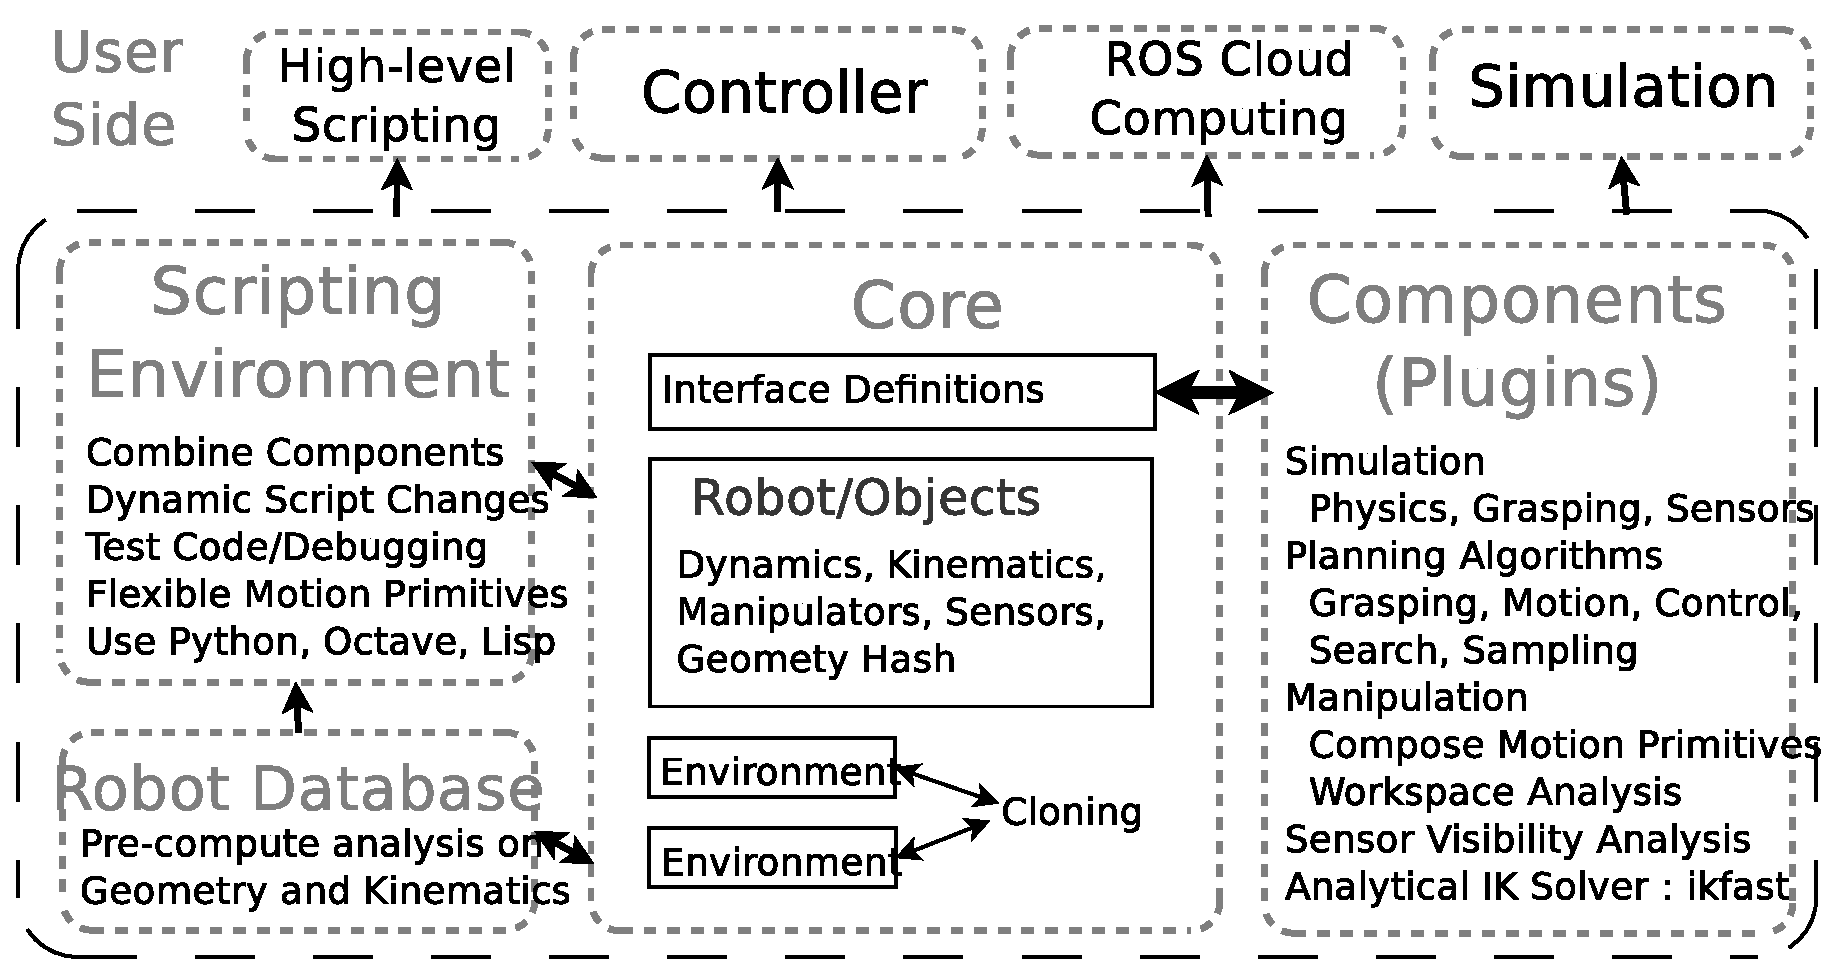
\includegraphics[width=15cm]{openrave_architecture}
\caption{OpenRAVE architecture}
\end{DoxyImage}


OpenRAVE is divided in four main components as shown in the above figure:


\begin{DoxyItemize}
\item {\bfseries Core Layer} The core is composed of a set of \hyperlink{group__interfaces}{Base Interface Classes} defining how plugins share information, and it provides an environment interface that maintains a world state, which serves as the gateway to all functions offered through OpenRAVE. The global openrave state manages the loaded plugins, multiple independent environments, and logging. On the other hand, the \hyperlink{classOpenRAVE_1_1EnvironmentBase}{environment} combines collision checkers, viewers, physics engines, the kinematic world, and all its interfaces into a coherent robotics world state.
\end{DoxyItemize}


\begin{DoxyItemize}
\item {\bfseries Plugins Layer} OpenRAVE is designed as a plugin-\/based architecture where a plugin offers implementations of the \hyperlink{group__interfaces}{Base Interface Classes} that are loaded dynamically into the \hyperlink{classOpenRAVE_1_1EnvironmentBase}{environment}. Plugins can be linked with other robotics libraries allowing \hyperlink{namespaceOpenRAVE}{OpenRAVE} to expand its functionality, or it can offer \hyperlink{namespaceOpenRAVE}{OpenRAVE} services to another robotics system. During startup, OpenRAVE parses the \{OPENRAVE\_\-PLUGINS\} environment variable and loads all the plugins it finds.
\begin{DoxyItemize}
\item Refer to \hyperlink{writing__plugins}{Writing Plugins and Interfaces} for a tutorial on how to build and compile plugins.
\item Refer to \hyperlink{interface__concepts}{Base Interface Concepts} for interface details.
\end{DoxyItemize}
\end{DoxyItemize}


\begin{DoxyItemize}
\item {\bfseries Scripting Layer} OpenRAVE provides scripting environments for \href{http://openrave.org/en/main/tutorials/openravepy_beginning.html#openravepy-beginning}{\tt Python} and \href{http://openrave.org/wiki/index.php/OctaveMATLAB}{\tt Octave/Matlab}. Python communicates with the core layer directly with in-\/memory calls, making it extremely fast. On the other hand, the Octave/Matlab scripting protocol send commands through TCP/IP, with a plugin offering a text server on the OpenRAVE core side. Scripting allows real-\/time modifications to any aspect of the environment without requiring shutdown, making it ideal to testing new algorithms. The Python scripting is so powerful, that most of the OpenRAVE examples and demo code are offered through it. In fact, users should treat the scripting language as an integral part of the entire system, not as a replacement to the C++ API.
\end{DoxyItemize}


\begin{DoxyItemize}
\item {\bfseries Robot Database Layer} Implements a planning knowledge-\/base and provides simple interfaces for its access and generation parameters. The database itself mostly consists of kinematic, quasi-\/static, dynamic, and geometric analyses of the robot and the task. If the robot is defined properly, then all these functions should work out of the box.
\end{DoxyItemize}

All the base planners and modules should be applicable to any robot structure that can be thrown at it. One of OpenRAVE's strongest points when compared with other planning packages is the idea of being able to apply algorithms in openrave to any robot, with very little modification. Recently, a planning database structure has been introduced that allows computation of properties like convex hull decomposition, grasp sets, reachability maps, analytic inverse kinematics, etc. If the robot is defined properly, then all these functions should work out of the box.

The main API is coded in C++ using the Boost C++ libraries \mbox{[}Dawes et al (1998-\/ present)\mbox{]} as a really solid basis of low-\/level management and storage structures. The Boost flavors of shared pointers allow object pointers to be safely reference counted in a heavily multi-\/threaded environment. Shared pointers also allow handles and interfaces to be passed to the user without having to every worry about the user calling upon invalid objects or un-\/ loaded shared objects. Furthermore, \hyperlink{namespaceOpenRAVE}{OpenRAVE} uses functors and other abstracted objects commonly seen in higher level languages to specify function pointers for sampling distri-\/ butions, event callbacks, setting robot configuration state, etc. The Boost-\/enabled design makes the the C++ API really safe and reliable to use along with saving the users a lot of trouble doing bookkeeping on their end. Furthermore, it allows the Resource Acquisition Is Initialization (RAII) design pattern \mbox{[}Stroustrup (2001)\mbox{]} to be fully exploited allowing users to ignore the complexities of multi-\/threaded resource management.\hypertarget{architecture__concepts_arch_environment}{}\subsection{Environment Concepts}\label{architecture__concepts_arch_environment}
All of OpenRAVE's services are offered through the environment. For example, requesting a planner interface called 'BiRRT' is done through RaveCreatePlanner(). The environment supports:


\begin{DoxyItemize}
\item \hyperlink{namespaceOpenRAVE_global_functionality}{managing and communicating with plugins}
\item \hyperlink{classOpenRAVE_1_1EnvironmentBase_env_collision_checking}{collision checking}
\item \hyperlink{classOpenRAVE_1_1EnvironmentBase_env_loading}{loading scenes and objects}
\item \hyperlink{classOpenRAVE_1_1EnvironmentBase_env_objects}{managing objects and triangulation}
\item \hyperlink{classOpenRAVE_1_1EnvironmentBase_env_plotting}{drawing/plotting}
\end{DoxyItemize}

Whenever objects in the environment are written or read, the user has to {\bfseries lock} the environment mutex mutex GetMutex(). This prevents any other process from modifying the enviornment while the user is working. Because the environment uses 'recursive mutexes, it allows a mutex to be locked as many times as needed within the same thread. This has allowed all environment functions that require locking to always guarantee the mutex is locked, regardless if the user has locked the mutex. (Note that this only applies to environment functions, and not interface functions).\hypertarget{architecture__concepts_arch_locking}{}\subsubsection{Locking}\label{architecture__concepts_arch_locking}
Because OpenRAVE is a highly multi-\/threaded environment, the environment state like bodies and loaded interfaces could be simultaneously accessed. In order to safely write or read the state, a user has to lock the environment, which prevents any other process from modifying the environment while the user is working. By using recursive locks, it allows a lock to be locked as many times as needed within the same thread, greatly reducing the lock management when a state changing function calls another state changing function. This safety measure helps users by always guaranteeing the environment is locked when calling global level environment functions like creating new bodies or loading scenes, regardless if the user has locked it. However, directly accessing the bodies and robots is dangerous without having the environment lock acquired.\hypertarget{architecture__concepts_arch_simulation}{}\subsubsection{Simulation Thread}\label{architecture__concepts_arch_simulation}
Every environment has an internal time and a simulation thread directly attached to a physics engine. The thread is always running in the background and periodically steps the simulation time by a small delta for the physics engine and on all the simulation-\/enabled interfaces. By default, the thread is always running and can always potentially modify the environment state; therefore, users always need to explicitly lock the environment whenever playing with the internal state like modifying bodies by setting joint values or link transformations. If not careful, the controller or physics engine will overwrite them. By default, the simulation thread just sets the object positions depending on their controller inputs, but a physics engine can be attached to integrate velocities, accelerations, forces, and torques.

The simulation thread can feel like a nuisance at first, but its division of robot control into control input computation and execution greatly helps users only concentrate on feeding commands to the robot without worrying about the simulation loop. It also allows a world update to happen in one one discrete time step.\hypertarget{architecture__concepts_arch_cloning}{}\subsubsection{Cloning}\label{architecture__concepts_arch_cloning}
One of the strengths of OpenRAVE is in allowing multiple \hyperlink{classOpenRAVE_1_1EnvironmentBase}{environments} work simultaneously in the same process. Environment cloning allows OpenRAVE to become truly parallel by managing multiple environments and running simultaneous planners on top of them.

One of the strengths of \hyperlink{namespaceOpenRAVE}{OpenRAVE} is in allowing multiple environments to work simul-\/ taneously in the same process. Environment cloning allows \hyperlink{namespaceOpenRAVE}{OpenRAVE} to become truly parallel by managing multiple environments and running simultaneous planners on top of them. Because there is no shared state across the clone and the original environment, it is not possible to use an interface created from one environment in another For example, if a planner is created in one environment, it should be used only by objects in that environment. It is not possible to set a planner to plan for objects belonging to a different environment. This is because a planner will lock the environment and expect the objects it controls to be exclusively under its control.

Creating a clone is simple, in C++ just type:


\begin{DoxyCode}
EnvironmentBasePtr pNewEnvironment = GetEnv()->CloneSelf(Clone_Bodies)
\end{DoxyCode}


to create a clone that copies all the existing bodies (with attachments and grabbed bodies) and their current states. Basically the clone can perform any operations that would have been done with the original enviornment.

Because the environment state is very complex, the cloning process can control how much of it gets transferred to the new clone. For example, all existing bodies and robots can be cloned, their attached controllers can be cloned, the attached viewer can be cloned, the collision checker state can be cloned, and the simulation state can be cloned. Basically the clone should be able to perform any operations that can be done with the original environment without any modification in the input parameters.

When cloning real robots, one extremely important feature that \hyperlink{namespaceOpenRAVE}{OpenRAVE} cloning offers is the ability to maintain a real-\/time view of the world that sensors continuously update with new information. When a planner is instantiated, it should make a copy of the environment that it can exclusively control without interfering with the updating operations. Furthermore, the real-\/world environment possibly has robot controllers connected to real robots, having a clone gives the ability to set simulation controllers guarantees robot safety while planning; commands from a cloned environment would not accidentally send commands to the real robot.\hypertarget{architecture__concepts_arch_validating_plugins}{}\subsubsection{Validating Plugins}\label{architecture__concepts_arch_validating_plugins}
Every plugin needs to export several functions to notify the core what interfaces it has and to instantiate the interfaces. When a plugin is first loaded, it is validated by the environment and its interface information is queried so the core can register the names.

There are many mechanisms in the validation process to prevent old plugins to be loaded by the core. \hyperlink{namespaceOpenRAVE}{OpenRAVE} is updated frequently and all user plugins are not necessarily recompiled when the \hyperlink{namespaceOpenRAVE}{OpenRAVE} API changes. Therefore, we will encounter many cases when a plugin exports the correct functions, but does not implement the correct API. Using interfaces from plugins compiled with a mismatching The API can lead to unexpected crashes that are very difficult to debug, so it is absolutely necessary to detect this condition. One possible solution is to add version numbers to the API to enforce checking before an interface is returned from the plugin to the environment, but this method is brittle. It forces to keep track of a version number for every interface along with a global version number. Furthermore, every developer has to remember to increment the version when something even small changes, which can be easily forgotten and lead to serious errors later on.

We solve interface validation by computing a unique hash of the interface functions and members by running each interface through a C++ lexer, gathering the tokens that affect the C++ code structure, and then creating a 128bit unique MD5 hash. We create a hash for each interface definition and the environment. The hashes are hard coded into the C++ header files and can be queried by two methods: a static function returning the hash of the program calling the function, and a virtual function returning the hash the interface was compiled with. An interface is only valid if its virtual hash is equivalent to the static hash of the core environment. For a plugin to be loaded correctly, first the environment hashes have to match. If they do, then the individual interfaces checked and only matching interfaces are returned to the core, and from there dispatched to other plugins. Such consistency checks ensure that stale plugins will never be loaded.\hypertarget{architecture__concepts_arch_cloning_parallel}{}\subsubsection{Parallel Execution}\label{architecture__concepts_arch_cloning_parallel}
Being able to execute a planner in multiple threads is important for applications that require speed and solution quality Because there is always a trade-\/off between solution quality and time of computation, some applications like industrial robots require the quickest and smoothest past to their destinations. Fortunately, environment cloning allows planners to create an independent environment for every thread they create, which enables them to call kinematics and collision functions in each respective thread without worrying about data corruption. Growing an RRT tree in a multi-\/threaded environment just requires one copy of the kd-\/tree structure to be maintained. The query operations mostly work with Euclidean distance on the configuration space, so are really fast. Furthermore, adding a new point takes O(log) time, so it shouldn’t be a bottleneck in the search process compared to collision checking. Finally, environment locking allows threads to gain exclusive access to the environment. The rule of thumb is that any interface belonging or added to the environment requires an environment lock before any of its methods can be called.\hypertarget{architecture__concepts_arch_dualnature}{}\subsection{Dual Simulation/Control Nature}\label{architecture__concepts_arch_dualnature}
\hyperlink{namespaceOpenRAVE}{OpenRAVE} can be simultaneously used as a simulation, a controller, or both at the same time. Here are a couple of things to keep in mind:


\begin{DoxyItemize}
\item It can be used as a simulator by attaching a physics engine and setting torques to the joints and applying forces to the links.
\end{DoxyItemize}


\begin{DoxyItemize}
\item The physics engine directly reflects the internal openrave state.
\end{DoxyItemize}


\begin{DoxyItemize}
\item A controller can be set that sets torques/velocities/positions to the physics engine every time step. Physics simulation time steps are constantly called in an internal \char`\"{}openrave thread\char`\"{} if simulations are set to true (default)
\end{DoxyItemize}


\begin{DoxyItemize}
\item The default physics engine doesn't touch the openrave state, nor does it simulate velocities or dynamics
\end{DoxyItemize}


\begin{DoxyItemize}
\item The default controller just sets positions at the specified times
\end{DoxyItemize}

This is why users need to explicitly lock the environment mutex whenever playing with the internal openrave state like setting joint values or link transformations (in planners for example). Otherwise, the controller or physics engine will overwrite them.\hypertarget{architecture__concepts_arch_exceptions}{}\subsection{Exception Handling}\label{architecture__concepts_arch_exceptions}
By using the C++ Standard and Boost libraries, \hyperlink{namespaceOpenRAVE}{OpenRAVE} can recover from almost all errors that a user can experience without causing the program to shutdown on the spot. Invalid pointer and out-\/of-\/range accesses are extremely dangerous because they can modify unrelated memory, which causes the program to crash at a place completely unrelated to the root cause of the problem. Avoiding such problems has been one of the the highest priorities for the design. The core always surrounds any user code coming from plugins and callbacks with try/catch blocks, this allows the core to properly handle the error and notify the user of a problem without tearing down the environment. Because exception handling is slow, there is a fine balance of when a function should return an error code and what it should throw an exception. In \hyperlink{namespaceOpenRAVE}{OpenRAVE}, exceptions should never occur in normal operation of the program, they should only be for unexpected events of the program. For example, planners failing is an expected event dependent on the current environment, so planners should return an error code with the cause of the failure rather than throw an exception. In other words, exceptions convey the structural errors of the program that point to places in the code that should be fixed by the user. The following operations should throw exceptions in \hyperlink{namespaceOpenRAVE}{OpenRAVE}:


\begin{DoxyItemize}
\item invalid plugin or interface hashes,
\item invalid commands being sent to interfaces,
\item invalid arguments passed to functions,
\item invalid pointers or out-\/of-\/range parts of lists are accessed,
\item environment is not locked when it should be
\item a resource is present when it should be,
\item a math operation is not consistent with the rest of the environment,
\item environment naming constraints are not maintained,
\item unrecognized enumerated types are given, and
\item instantiation order is not maintained.
\end{DoxyItemize}

Any type of boost error, or null pointer access throws an openrave\_\-exception. This greatly reduces the amount of error checking code people do. For example, C code usually has this pattern:


\begin{DoxyCode}
bool somefun(KinBodyPtr pbody)
{
    if( !pbody )
        return false;
    pbody->GetTransform();
    ...
}
\end{DoxyCode}


or


\begin{DoxyCode}
bool somefun(KinBodyPtr pbody)
{
    assert( !!pbody );
    pbody->GetTransform();
    ...
}
\end{DoxyCode}


If these checks are not done, the code would segfault. However, these checks can really clutter the code. In openrave, it is safe to get away with:


\begin{DoxyCode}
bool somefun(KinBodyPtr pbody)
{
    pbody->GetTransform();
    ...
}
\end{DoxyCode}


then for handling errors (for example in the most top-\/level script), do


\begin{DoxyCode}
try {
    ...
    somefun(pbody)
    ...
}
catch(const openrave_exception& ex) {
    RAVELOG_WARN("exception caught: %s\n",ex.what());
    if( ex.GetCode() == ORE_EnvironmentNotLocked ) {
        RAVELOG_WARN("user forgot to lock environment!\n");
    }
    ...
}
\end{DoxyCode}


When using openravepy in python, such unhandled C++ errors throw a python exception, which can be safely caught and processed there.\hypertarget{architecture__concepts_arch_body_hashes}{}\subsection{Hashes for Body Structure}\label{architecture__concepts_arch_body_hashes}
A new concept that came out of \hyperlink{namespaceOpenRAVE}{OpenRAVE} is the idea of creating unique hashes of a body’s structure. Every body has an online state that includes:


\begin{DoxyItemize}
\item names of the body, its links, its joints,
\item link transformations, velocities, and accelerations in the world,
\item and attached bodies.
\end{DoxyItemize}

All other information is independent of the environment and can be categorized into the kinematics, geometry, and dynamics of the body. Furthermore, robots have categories for attached sensors and manipulators. The planning knowledge-\/base stores all cached information about a body and a robot, so it needs an consistent way of indexing this information. Indexing by robot names is not reliable because it is very difficult to remind a user to change the name every time the body structure is changed. Therefore, \hyperlink{namespaceOpenRAVE}{OpenRAVE} provides functionality to serialize the different categories of a body and create a 128-\/bit MD5 hash. Each of the models in the planning knowledge-\/base relies on different categories of the robot. For example:


\begin{DoxyItemize}
\item inverse kinematics generation only uses the kinematics of a sub-\/chain of the robot defined by the manipulator and the grasp coordinate system,
\item kinematic reachability cares about the robot geometry of the manipulator because it implicitly stores self-\/collision results,
\item inverse reachability further uses the links connecting the base robot link to the base manipulator link,
\item grasping cares about the geometry of the target body and the kinematics and geometry of the gripper,
\item convex decompositions only care about the link geometry, and
\item inverse dynamics cares only about the dynamics properties of each link and the kinematics.
\end{DoxyItemize}

There are several challenges to developing a consistent index across all operating systems and compilers since floating point errors could creep in when normalizing floating-\/point values. However, the idea of such an index could greatly help in developing a worldwide robot database that anyone can use.\hypertarget{architecture__concepts_supported_formats}{}\subsection{Resource File Formats}\label{architecture__concepts_supported_formats}
\hyperlink{namespaceOpenRAVE}{OpenRAVE} defines its own  format that allows instantiation of any \hyperlink{namespaceOpenRAVE}{OpenRAVE} interface and quick builing of robots and and kinematics structures. The rigid body geometries resources can be specified in virtually any 3D file format. For example:


\begin{DoxyItemize}
\item iv, vrml, wrl, stl, blend, 3ds, ase, obj, ply, dxf, lwo, lxo, ac, ms3d, x, mesh.xml, irrmesh, irr, nff, off, raw
\end{DoxyItemize}

These files can be used inside the $<$geom$>$ tags, or can be read directly into any of the environment ReadRobotX and ReadKinBodyX methods to create a single world body.

\hyperlink{namespaceOpenRAVE}{OpenRAVE} also supports the \href{http://www.collada.org}{\tt COLLADA} international standard on 3D geometry and modeling. COLLADA is augmented with these \href{http://openrave.programmingvision.com/wiki/index.php/Format:COLLADA}{\tt OpenRAVE robot-\/specific extensions}.

\href{../main/robots_overview.html#file-formats}{\tt More information here.} 
\clearemptydoublepage
\section{Base Interface Concepts}
\label{interface_concepts}
\hypertarget{interface_concepts}{}
New interfaces are provided by plugins and are dynamically loaded into OpenRAVE. All interfaces are derived from the \hyperlink{classOpenRAVE_1_1InterfaceBase}{OpenRAVE::InterfaceBase} class and contain basic information such as the type, the owning \hyperlink{classOpenRAVE_1_1EnvironmentBase}{environment}, setting user data, cloning, and allowing custom string commands to be sent.

Every instantiated interface belongs to only one \hyperlink{classOpenRAVE_1_1EnvironmentBase}{environment}. Interfaces can be cloned using \hyperlink{classOpenRAVE_1_1InterfaceBase_aadffdb83bc22dcdd5dd50c27d1bb5496}{OpenRAVE::InterfaceBase::Clone}.

Every interface can have its own custom commands. Sending {\bfseries help} will return a list of all the commands the interface supports (think of it as a command-\/line way of sending commands to the interface). The GetDescription() returns a string briefly explaining the functionality, the authors, and the license of the plugin.

Ability to register custom xml reader interfaces.


\begin{DoxyItemize}
\item \hyperlink{arch__collisionchecker}{Collision Checker Concepts}
\item \hyperlink{arch__controller}{Controller Concepts}
\item \hyperlink{arch__iksolver}{Inverse Kinematics Solver Concepts}
\item \hyperlink{arch__kinbody}{Kinematics Body Concepts}
\item \hyperlink{arch__physicsengine}{Physics Engine Concepts}
\item \hyperlink{arch__planner}{Planner Concepts}
\item \hyperlink{arch__module}{Module Concepts}
\item \hyperlink{arch__robot}{Robot Concepts}
\item \hyperlink{arch__sensor}{Sensor Concepts}
\item \hyperlink{arch__sensorsystem}{Sensor System Concepts}
\item \hyperlink{arch__spacesampler}{SpaceSampler Concepts}
\item \href{../main/architecture/trajectory.html}{\tt Trajectory Concepts}
\item \hyperlink{arch__viewer}{Viewer Concepts} 
\end{DoxyItemize}\hypertarget{arch_collisionchecker}{}\subsection{Collision Checker Concepts}\label{arch_collisionchecker}
{\bfseries Reference:} \hyperlink{classOpenRAVE_1_1CollisionCheckerBase}{OpenRAVE::CollisionCheckerBase}.

All {\bfseries CheckCollision} functions accept an optional pointer to a \hyperlink{classOpenRAVE_1_1CollisionReport}{OpenRAVE::CollisionReport} struct, which gets filled with information about the collision that takes place. Usually requesting more precise information like distance to obstacles is computationally expensive; therefore to save computation, the user can specify what collision information should be filled in the \hyperlink{classOpenRAVE_1_1CollisionReport}{OpenRAVE::CollisionReport} with the SetCollisionOptions function.

\hyperlink{namespaceOpenRAVE}{OpenRAVE} is not tied to a particular collision checker. Collision checkers can be changed with SetCollisionChecker. In order to add a new collision checker, derive a class from \hyperlink{classOpenRAVE_1_1CollisionCheckerBase}{OpenRAVE::CollisionCheckerBase} and fill all the methods it provides. Then register it in 'src/environment.cpp' and CollisionCheckers. All collision checking is done through the overloaded EnvironmentBase::CheckCollision. \hypertarget{arch_controller}{}\subsection{Controller Concepts}\label{arch_controller}
{\bfseries Reference:} \hyperlink{classOpenRAVE_1_1ControllerBase}{OpenRAVE::ControllerBase}

In order for openrave to control certain robot hardware, a \hyperlink{classOpenRAVE_1_1ControllerBase}{OpenRAVE::ControllerBase} controller has to be created that will interface with the hardware-\/specific libraries. This controller interface then has to be created through the environment and set onto an existing robot. All commands given to the robot are first filtered through the controller, then translated to joint commands. Different controllers can have different path inputs (ie: a robot walking on a floor might just have x,y,angle), but the default is the DOF joint values.\hypertarget{arch__controller_arch_controller_writing}{}\subsubsection{Writing and Using Controllers}\label{arch__controller_arch_controller_writing}
Assuming that there exists a plugin with a controller interface named {\bfseries MyController}, here are some ways to set an openrave robot to use it:


\begin{DoxyItemize}
\item XML
\begin{DoxyItemize}
\item add a {\bfseries } $<$controller$>$ tag in the openrave robot XML file like this: \begin{DoxyVerb}
<robot file="robots/schunk-lwa3.robot.xml">
  <controller type="MyController controller arguments here"></controller>
</robot>
\end{DoxyVerb}

\item It is also possible to set a controller outside of the robot definition by specifying the robot's name. For example: \begin{DoxyVerb}
<environment>
  <robot name="schunk-lwa3" file="robots/schunk-lwa3.robot.xml">
  </robot>
  <controller type="MyController" robot="schunk-lwa3 controller arguments here"></controller>
  </environment>
\end{DoxyVerb}

\end{DoxyItemize}
\end{DoxyItemize}


\begin{DoxyItemize}
\item C++ 
\begin{DoxyCode}
RobotBasePtr probot = GetEnv()->GetRobot("schunk-lwa3");
ControllerBasePtr pcontroller = RaveCreateController(GetEnv(),"MyController contr
      oller arguments here");
vector<int> dofindices(probot->GetDOF());
for(int i = 0; i < probot->GetDOF(); ++i) {
    dofindices[i] = i;
}
int nControlTransformation = 1;
probot->SetController(pcontroller,dofindices,nControlTransformation);
\end{DoxyCode}

\end{DoxyItemize}


\begin{DoxyItemize}
\item Python 
\begin{DoxyCode}
robot = env.GetRobot('schunk-lwa3')
controller = RaveCreateController(env,'MyController controller arguments here')
robot.SetController(controller,range(robot.GetDOF()),controltransform=1)
\end{DoxyCode}

\end{DoxyItemize}


\begin{DoxyItemize}
\item Octave/MATLAB \begin{DoxyVerb}
robotid = orEnvGetBody('schunk-lwa3');
orRobotControllerSet(robotid,'MyController','controller arguments here')
\end{DoxyVerb}
 
\end{DoxyItemize}\hypertarget{arch_iksolver}{}\subsection{Inverse Kinematics Solver Concepts}\label{arch_iksolver}
{\bfseries Reference:} \hyperlink{classOpenRAVE_1_1IkSolverBase}{OpenRAVE::IkSolverBase}

Each IK solver is defined on a subset of joints of a Robot specified by the robot's manipulator. Given the position in the 3D workspace that an end effector should go to, an IK solver will find the joint configuration to take that end-\/effector there. Because it is common for an IK solution to have a null space, the IK solver give functionality to expose the free parameters to move the joints in null space. \hypertarget{arch_kinbody}{}\subsection{Kinematics Body Concepts}\label{arch_kinbody}
{\bfseries Reference:} \hyperlink{classOpenRAVE_1_1KinBody}{OpenRAVE::KinBody}

Each KinBody can be thought of as the basic rigid body element in \hyperlink{namespaceOpenRAVE}{OpenRAVE}. It is composed of a collection of links (rigid bodies) connected with joints. The KinBody class provides a lot of functionality (from a planning perspective) needed to perform complex tasks:


\begin{DoxyItemize}
\item Setting and getting joint values
\item Setting and getting the transformations of all links
\item Getting the velocities of each joint (or link)
\item Self collision detection functions
\item Kinematic hierarchy querying -\/ The underlying structure of KinBody is a list of links, not a tree. However, after some careful analysis, the parent and child links of a particular link can be extracted.
\item Jacobian calculation -\/ both translational and rotational.
\item Attaching bodies online -\/ a necessary function for manipulation planning; is called, for example, when an object is rigidly grasped by a hand
\end{DoxyItemize}\hypertarget{arch__kinbody_arch_kinbody_options}{}\subsubsection{Loading Options}\label{arch__kinbody_arch_kinbody_options}
This is the set of loading options passed as a AttributesList into functions like OpenRAVE::EnvironmentBase::ReadKinBodyXMLFile:
\begin{DoxyItemize}
\item {\bfseries prefix}: prefix link, joint, manipulator, and sensor names with a string
\item {\bfseries skipgeometry}: if 1 or true, will skip loading all geometry of the links 
\end{DoxyItemize}\hypertarget{arch_physicsengine}{}\subsection{Physics Engine Concepts}\label{arch_physicsengine}
{\bfseries Reference:} \hyperlink{classOpenRAVE_1_1PhysicsEngineBase}{OpenRAVE::PhysicsEngineBase}

The physics engine for the environment can be set through \hyperlink{classOpenRAVE_1_1EnvironmentBase_a4b682d62526e5840d8fdc25343ee563c}{OpenRAVE::EnvironmentBase::SetPhysicsEngine}. \hypertarget{arch_planner}{}\subsection{Planner Concepts}\label{arch_planner}
{\bfseries Reference:} \hyperlink{classOpenRAVE_1_1PlannerBase}{OpenRAVE::PlannerBase}\hypertarget{arch__planner_planner_intro}{}\subsubsection{Introduction}\label{arch__planner_planner_intro}
In \hyperlink{namespaceOpenRAVE}{OpenRAVE}, the basic purpose of a planner is to find a trajectory starting at some initial configuration that reaches a goal condition while satisfying various navigation constraints. All planners are assumed to be geometric in nature (ie, not planning in the space of policies that depend on sensor data). Planners can have any configuration space defined by using the \hyperlink{classOpenRAVE_1_1PlannerBase_1_1PlannerParameters}{OpenRAVE::PlannerBase::PlannerParameters} structure. A planner should never use the raw joint values functions defined in KinBody.

The usage of a planner is simple:


\begin{DoxyItemize}
\item Acquire its pointer from RaveCreatePlanner.
\end{DoxyItemize}


\begin{DoxyItemize}
\item Fill a \hyperlink{classOpenRAVE_1_1PlannerBase_1_1PlannerParameters}{PlannerParameters} structure defining the instance of the problem. The structure has many fields for describing planning entities like start position, goal condition, and the distance metric. Try to use these fields as much as possible. Later on, this will allow users to easily swap planners without having to change the PlannerBase::PlannerParameters structure much.
\end{DoxyItemize}


\begin{DoxyItemize}
\item Call \hyperlink{classOpenRAVE_1_1PlannerBase_a109c37d3de7ee99f93c740a2df0e5e34}{InitPlan} passing in the robot and planner parameters. This also resets any previous information the planner had stored.
\end{DoxyItemize}


\begin{DoxyItemize}
\item Call \hyperlink{classOpenRAVE_1_1PlannerBase_a7ce22311b1f81ec6b9bacdf457d4631a}{PlanPath} passing in a \hyperlink{classOpenRAVE_1_1TrajectoryBase}{trajectory} (and optionally an output stream) to start planning. If the function returns true, then the Trajectory will be filled with the geometric solution in the active DOF configuration space of the robot. By calling SetParameters, then PlanPath again, it could be possible to preserve the previous search space for the planner while changing the goal conditions.
\end{DoxyItemize}\hypertarget{arch__planner_planner_planning}{}\subsubsection{Planning Details}\label{arch__planner_planner_planning}
\hypertarget{arch__planner_planner_parameters}{}\paragraph{Planner Parameters -\/ Calling a Planner}\label{arch__planner_planner_parameters}
All the information defining a planning problem should be specified in PlannerBase::PlannerParameters. {\ttfamily PlannerParameters} tries to cover most of the common data like distance metrics, sampling distributions, initial and goal configurations. However there are many different types of inputs to a planner, so it is impossible to cover everything with one class. Instead, {\ttfamily PlannerParameters} has a very flexible and safe way to extend its parameters without destroying compatibility with a particular planner or user of the planner. This is enabled by the serialization to XML capabilities of {\ttfamily PlannerParameters}


\begin{DoxyCode}
PlannerBase::PlannerParametersPtr params(new PlannerBase::PlannerParameters());
params->vinitialconfig.push_back(2);
ostream os;
os << *params;
\end{DoxyCode}


will produce something in the form of \begin{DoxyVerb}
<PlannerParameters>
  <initialconfig>2</initialconfig>
</PlannerParameters>
\end{DoxyVerb}


Furthermore \hyperlink{classOpenRAVE_1_1PlannerBase_1_1PlannerParameters}{PlannerParameters} can read such an XML file given an input stream \begin{DoxyVerb}
istream is;
is >> *params;
\end{DoxyVerb}


Using XML as a medium, it is easy to exchange data across different derivations of \hyperlink{classOpenRAVE_1_1PlannerBase_1_1PlannerParameters}{PlannerParameters} without much effort. To add new parameters for planners to take advantage of


\begin{DoxyItemize}
\item make a derived class from \hyperlink{classOpenRAVE_1_1PlannerBase_1_1PlannerParameters}{PlannerParameters}
\item overload the \hyperlink{classOpenRAVE_1_1PlannerBase_1_1PlannerParameters_a2084222cd1b9f555406d306d65680d7b}{PlannerParameters}, startElement, endElement, and characters functions to process the new variables.
\end{DoxyItemize}

As long as the user of the planner passes a {\ttfamily PlannerParameters} that can serialize to the same format of data that the planner expects, the data will be passed. This allows the planner and the caller of \hyperlink{classOpenRAVE_1_1PlannerBase_a7ce22311b1f81ec6b9bacdf457d4631a}{PlanPath} to use different {\ttfamily PlannerParameters}. definitions without any conflicts.\hypertarget{arch__planner_planner_basicusage}{}\paragraph{Basic Usage}\label{arch__planner_planner_basicusage}
This is a simple call to a birrt planner, let {\bfseries activegoal} hold the goal configuration and {\bfseries activejoints} hold indices to the robot joints interested to plan for.


\begin{DoxyCode}
PlannerBase::PlannerParametersPtr params(new PlannerBase::PlannerParameters);
params->SetRobotActiveJoints(robot); // sets the active joint indices 
robot->GetActiveDOFValues(params.vinitialconfig); // set initial config (use curr
      ent robot configuration)
params.vgoalconfig = activegoal;
 
// set other params values like
 
PlannerBasePtr rrtplanner = RaveCreatePlanner(GetEnv(),"rBiRRT");
TrajectoryBasePtr ptraj = RaveCreateTrajectory(GetEnv(),robot->GetActiveDOF());
if( !rrtplanner->InitPlan(robot, params) ) {
    return false;
}

PlannerStatus status = rrtplanner->Plan(ptraj);
if( status & PS_HasSolution ) {
    robot->SetActiveMotion(ptraj); // trajectory is done, execute on the robot
}
\end{DoxyCode}


In order to speed up computations further, planners can use the CO\_\-ActiveDOFs collision checker option, which only focuses collision on the currently moving links in the robot. If using the robot active DOF, before calling the planner, the user should insert this statement:


\begin{DoxyCode}
CollisionOptionsStateSaver optionstate(GetEnv()->GetCollisionChecker(),GetEnv()->
      GetCollisionChecker()->GetCollisionOptions()|CO_ActiveDOFs,false);
\end{DoxyCode}
\hypertarget{arch__planner_planner_extraparameters}{}\paragraph{Defining Extra Planner Parameters}\label{arch__planner_planner_extraparameters}
Here is how to derive from a \hyperlink{classOpenRAVE_1_1PlannerBase_1_1PlannerParameters}{PlannerParameters} class in order to introduce new parameters.


\begin{DoxyCode}
class BasicRRTParameters : public PlannerBase::PlannerParameters
{
public:
BasicRRTParameters() : _fGoalBiasProb(0.05f), _bProcessing(false) {
        _vXMLParameters.push_back("goalbias");
    }
    
    dReal _fGoalBiasProb; 

 protected:
    bool _bProcessing;
    virtual bool serialize(std::ostream& O) const
    {
        if( !PlannerParameters::serialize(O) )
            return false;
        O << "<goalbias>" << _fGoalBiasProb << "</goalbias>" << endl;
        return !!O;
    }

    ProcessElement startElement(const std::string& name, const std::list<std::pai
      r<std::string,std::string> >& atts)
    {
        if( _bProcessing )
            return PE_Ignore;
        switch( PlannerBase::PlannerParameters::startElement(name,atts) ) {
            case PE_Pass: break;
            case PE_Support: return PE_Support;
            case PE_Ignore: return PE_Ignore;
        }
        
        _bProcessing = name=="goalbias";
        return _bProcessing ? PE_Support : PE_Pass;
    }
    
    virtual bool endElement(const string& name)
    {
        if( _bProcessing ) {
            if( name == "goalbias")
                _ss >> _fGoalBiasProb;
            else
                RAVELOG_WARN(str(boost::format("unknown tag %s\n")%name));
            _bProcessing = false;
            return false;
        }

        // give a chance for the default parameters to get processed
        return PlannerParameters::endElement(name);
    }
};
\end{DoxyCode}
\hypertarget{arch__planner_planner_development}{}\paragraph{Planner Development}\label{arch__planner_planner_development}
Most planners do their computation iteratively, and they take lots of computation time. It is very frequent for a user to want to early-\/terminate the planner, or tell it to return the best solution it has founds immediately. Users might also want to visualize the planning process without getting into the internals of the planner. In order to do this, \hyperlink{namespaceOpenRAVE}{OpenRAVE} allows users to register callbacks via \hyperlink{classOpenRAVE_1_1PlannerBase_a7b72116e4770d98f2a78297246a679e8}{OpenRAVE::PlannerBase::RegisterPlanCallback}. Planner developers should {\bfseries always} call \hyperlink{classOpenRAVE_1_1PlannerBase_a4b980a3cc0e8fc7abd2d0afe472ef695}{OpenRAVE::PlannerBase::\_\-CallCallbacks} inside their planning loop and process the input correctly.\hypertarget{arch__planner_planner_examples}{}\subsubsection{Planner Examples}\label{arch__planner_planner_examples}
Examples of planners are:
\begin{DoxyItemize}
\item Manipulation -\/ manipulable objects need to be specified. Objects like doors should be special cases that planners knows about.
\item Following -\/ Goal easily changes. Attributes can change.
\item Path Smoothing -\/ uses the input trajectory
\item Trajectory Re-\/timing -\/ uses the input trajectory
\item Object Building -\/ Need to describe how parts of object fit together into a bigger part.
\item Dish Washing -\/ Specific goals are not specified, just a condition that all plates need to be inside.
\item Foot step planning -\/ Need discrete footsteps and other capabilities from robot.
\end{DoxyItemize}

Planner should be able to query sensor information from the Robot like its current camera image etc. Planner should be compatible with Robot presented; some hand-\/shaking should happen between the two during InitPlan function.\hypertarget{arch__planner_planner_pathoptimization}{}\subsubsection{Path Optimization}\label{arch__planner_planner_pathoptimization}
Path smoothing/optimization can be regarded as a post-\/processing step to planners. \char`\"{}Path optimization\char`\"{} algorithms take in an existing trajectory and filter it using the existing constraints of the planner. In fact, functionality there is no difference between a \char`\"{}path optimization\char`\"{} planner and a regular planner besides the fact that a trajectory is used as input. Because PlannerBase::PlanPath already has a trajectory as an argument, this does not cause any major API changes to the infrastructure.

However, the PlannerParameters structure had to reflect what 'path optimization' algorithm to use for post processing the trajectory. This is now reflected in the PlannerParameters::\_\-sPostProcessingPlanner and PlannerParameters::\_\-sPostProcessingParameters arguments. By default, this is the default \char`\"{}linear shortcut\char`\"{} path optimizer. There is also a helper function in PlannerBase to help users easily call the post-\/processing step:


\begin{DoxyCode}
_ProcessPostPlanners(RobotBasePtr probot, TrajectoryBasePtr ptraj);
\end{DoxyCode}


Please take a look at how the default RRT algorithms are now structured.

Planner post-\/processing actually allows users to chain planners in the same way that filters are chained, all through specifying planner parameters. Of course, users can continue to smooth in planners without relying on this framework. However, explicit control of path smoothing allows custom parameter to be easily specified. \hypertarget{arch_module}{}\subsection{Module Concepts}\label{arch_module}
{\bfseries Reference:} \hyperlink{classOpenRAVE_1_1ModuleBase}{OpenRAVE::ModuleBase}

Base class for modules the user might want to instantiate. A module registers itself with OpenRAVE's SimulateStep calls and can accept commands from the server or other plugins via SendCommand. A module stops receiving commands when it is destroyed. Modules are an easy way for developers to run and test their own code. \hypertarget{arch_robot}{}\subsection{Robot Concepts}\label{arch_robot}
{\bfseries Reference:} \hyperlink{classOpenRAVE_1_1RobotBase}{OpenRAVE::RobotBase}

Robots are a special type of KinBody that need higher level functionality for their control and movement in the environment. There are a couple of differences between a Robot and a regular KinBody.\hypertarget{arch__robot_arch_robot_manipulator}{}\subsubsection{Manipulators}\label{arch__robot_arch_robot_manipulator}
Every robot supports a list of \hyperlink{classOpenRAVE_1_1RobotBase_1_1Manipulator}{Manipulator} objects that describe the links the robot should use when manipulating parts of the environment. Usually manipulators are serial chains with a Base link and an End Effector link. Each manipulator is also decomposed into two parts: the arm and the hand. The hand usually makes contact with the objects while the arm transfers the hand to its destination. The Manipulator class also has an optional pointer to a IkSolverBase class providing inverse kinematics functionality. The IK solver used by a Manipulator can be changed by Manipulator::SetIKSolver, so plugins can provide and set their own IK solvers.\hypertarget{arch__robot_arch_robot_activedof}{}\subsubsection{Active Degrees of Freedom}\label{arch__robot_arch_robot_activedof}
When controlling and planning for a robot, it is possible to set the degrees of freedom that should be used. For example, consider a humanoid robot. There should be in easy way to specify to planners that only the right hand of the robot should be taken into consideration when planning; the rest of the joints should be ignored. Or consider the case where we care about navigation of the humanoid robot. Here we would want to control the translation of the robot on the plane and its orientation. Perhaps we want to do footstep planning and also care about controlling the two legs. All this is possible with the Active Degrees of Freedom feature provided by \hyperlink{namespaceOpenRAVE}{OpenRAVE}. First call RobotBase::SetActiveDOFs to set the degrees of freedom of the robot; it is also possible to set translation about the XYZ axes or the angle around a rotation axis as a degree of freedom. Each RobotBase function with the word Active expects the active DOF values to be specified. Basically, for any function in KinBody that deals with Joints, there is a corresponding active function in RobotBase.\hypertarget{arch__robot_arch_robot_grabbing}{}\subsubsection{Grabbing Bodies}\label{arch__robot_arch_robot_grabbing}
It is possible for a robot to attach a \hyperlink{classOpenRAVE_1_1KinBody}{KinBody} onto one of its links so that when the link moves, the KinBody also moves. Because collision detection will stop being checked between the robot and the KinBody, you could say that the KinBody becomes a part of the robot temporarily. This functionality is necessary for manipulation planning. Whenever the robot is carrying a body, all collisions between the robot and that item should be ignored once the body has been grasped.\hypertarget{arch__robot_arch_robot_sensors}{}\subsubsection{Attaching Sensors}\label{arch__robot_arch_robot_sensors}
Can attach any number of sensors to the robot's links through the \hyperlink{classOpenRAVE_1_1RobotBase_1_1AttachedSensor}{AttachedSensor} class. The sensor transformation will be completely owned by the robot. A robot can be attached with any number of sensors on any number of links. As the robot link moves, the sensor moves with it preserving its relative transformation.

AttachedSensor object holds a \hyperlink{classOpenRAVE_1_1SensorBase}{SensorBase} object that contains the actual object gathering and publishing data.\hypertarget{arch__robot_arch_robot_options}{}\subsubsection{Loading Options}\label{arch__robot_arch_robot_options}
This is the set of loading options passed as a AttributesList into functions like OpenRAVE::EnvironmentBase::ReadRobotXMLFile.

KinBody \hyperlink{arch__kinbody_arch_kinbody_options}{Loading Options} is also valid. \hypertarget{arch_sensor}{}\subsection{Sensor Concepts}\label{arch_sensor}
{\bfseries Reference:} \hyperlink{classOpenRAVE_1_1SensorBase}{OpenRAVE::SensorBase}

A sensor measures physical properties from the environment and converts them to data. Each sensor is associated with a particular position in space, has a geometry with properties defining the type of sensor, and can be queried for sensor data. Available sensor types are specified by SensorType.

By default, all the sensors start with power off, meaning that the sensor does not gather data. The power can be turned on by using \hyperlink{classOpenRAVE_1_1SensorBase_ae02c7c4987dd11f5fb7657e18c7c8318}{OpenRAVE::SensorBase::Configure} and sending the SensorBase::CC\_\-PowerOn command. All programs should manually turn sensor power on before using the sensors.

The sensor has two different rendering options:.


\begin{DoxyItemize}
\item {\bfseries Geometry Rendering} -\/ Renders a small icon that represents where the laser is placed in the environment, the icon's image should only be dependent on the geometry parameters of the sensor, and not the actual sensor data. Geometry rendering should be turned on by default. To configure this, use the SensorBase::CC\_\-RenderDataX commands.
\end{DoxyItemize}


\begin{DoxyItemize}
\item {\bfseries Data Rendering} -\/ Data rendering shows the measured sensor data coming out of the GetSensorData(). Usually the data can be very heavy, especially when a sensor's update rate is high, so data rendering is turned off by default. If the power is off, data should not be rendered. To configure this, use the SensorBase::CC\_\-RenderGeometryX commands.
\end{DoxyItemize}

Check out the \href{../main/plugins.html#basesensors}{\tt basesensors} plugin for an example of how to implement a basic laser range and camera sensors. \hypertarget{arch_sensorsystem}{}\subsection{Sensor System Concepts}\label{arch_sensorsystem}
{\bfseries Reference:} \hyperlink{classOpenRAVE_1_1SensorSystemBase}{OpenRAVE::SensorSystemBase} New objects can be created, existing objects can be updated. Every managed object should set the kinbody's Manager pointer \hypertarget{arch_spacesampler}{}\subsection{SpaceSampler Concepts}\label{arch_spacesampler}
{\bfseries Reference:} \hyperlink{classOpenRAVE_1_1SpaceSamplerBase}{OpenRAVE::SpaceSamplerBase}

Space samplers are responsible for generating samples in spaces like R$^\wedge$n, SO(3), SE(3), etc. The samples can be randomized or deterministic.

Each sampler can support returning the values in a floating-\/point precision or unsigned integer format. There are sampling calls for each version. The samplers could choose to implement only one of the types of both, this should be clear in the Supports function.

Each sampler has a state and can be configured with different dimensions and seeds. \hypertarget{arch_viewer}{}\subsection{Viewer Concepts}\label{arch_viewer}
{\bfseries Reference:} \hyperlink{classOpenRAVE_1_1ViewerBase}{OpenRAVE::ViewerBase} Viewer is responsible only for the environment it is attached to. 
\clearemptydoublepage
\section{Module Documentation}
\hypertarget{group__plugin__exports}{
\subsection{Plugin Export Functions}
\label{group__plugin__exports}\index{Plugin Export Functions@{Plugin Export Functions}}
}
\subsubsection*{Classes}
\begin{DoxyCompactItemize}
\item 
class \hyperlink{classOpenRAVE_1_1PLUGININFO}{PLUGININFO}
\begin{DoxyCompactList}\small\item\em Holds all the OpenRAVE-\/specific information provided by a plugin. \item\end{DoxyCompactList}\end{DoxyCompactItemize}
\subsubsection*{Typedefs}
\begin{DoxyCompactItemize}
\item 
\hypertarget{group__plugin__exports_ga6ae2f1554f547f27e4a5399d8aef7377}{
typedef InterfaceBasePtr($\ast$ \hyperlink{group__plugin__exports_ga6ae2f1554f547f27e4a5399d8aef7377}{PluginExportFn\_\-OpenRAVECreateInterface} )(InterfaceType type, const std::string \&name, const char $\ast$pluginhash, const char $\ast$envhash, EnvironmentBasePtr penv)}
\label{group__plugin__exports_ga6ae2f1554f547f27e4a5399d8aef7377}

\begin{DoxyCompactList}\small\item\em Create the interfaces, see \hyperlink{group__plugin__exports_ga468c900067e08689383b3f8da642141f}{CreateInterfaceValidated}. \item\end{DoxyCompactList}\item 
\hypertarget{group__plugin__exports_ga7cb4e2769bee1dca182b4432a900bc70}{
typedef bool($\ast$ \hyperlink{group__plugin__exports_ga7cb4e2769bee1dca182b4432a900bc70}{PluginExportFn\_\-OpenRAVEGetPluginAttributes} )(PLUGININFO $\ast$pinfo, int size, const char $\ast$infohash)}
\label{group__plugin__exports_ga7cb4e2769bee1dca182b4432a900bc70}

\begin{DoxyCompactList}\small\item\em Called to fill information about the plugin, see \hyperlink{group__plugin__exports_gaf90c03438b94cc76e7b8a54d445ec106}{GetPluginAttributesValidated}. \item\end{DoxyCompactList}\item 
\hypertarget{group__plugin__exports_ga7164d2e9a268c6e44a296e9488df69cd}{
typedef void($\ast$ \hyperlink{group__plugin__exports_ga7164d2e9a268c6e44a296e9488df69cd}{PluginExportFn\_\-DestroyPlugin} )()}
\label{group__plugin__exports_ga7164d2e9a268c6e44a296e9488df69cd}

\begin{DoxyCompactList}\small\item\em Called before plugin is unloaded from openrave. See \hyperlink{group__plugin__exports_gad6773d91dae37d0ba9de59d2a05277e4}{DestroyPlugin}. \item\end{DoxyCompactList}\end{DoxyCompactItemize}
\subsubsection*{Functions}
\begin{DoxyCompactItemize}
\item 
OpenRAVE::InterfaceBasePtr \hyperlink{group__plugin__exports_ga468c900067e08689383b3f8da642141f}{CreateInterfaceValidated} (OpenRAVE::InterfaceType type, const std::string \&name, std::istream \&sinput, OpenRAVE::EnvironmentBasePtr penv)
\begin{DoxyCompactList}\small\item\em {\bfseries {\bfseries }\mbox{[}helper\mbox{]}} Validated function callback for creating an interface function. No checks need to be made on the parmaeters. \item\end{DoxyCompactList}\item 
void \hyperlink{group__plugin__exports_gaf90c03438b94cc76e7b8a54d445ec106}{GetPluginAttributesValidated} (\hyperlink{classOpenRAVE_1_1PLUGININFO}{OpenRAVE::PLUGININFO} \&info)
\begin{DoxyCompactList}\small\item\em {\bfseries {\bfseries }\mbox{[}helper\mbox{]}} Validated function callback for returning a plugin's information. No checks need to be made on the parmaeters. \item\end{DoxyCompactList}\item 
\hypertarget{group__plugin__exports_ga6251cc7d3b33f6109ca5d346def08370}{
OPENRAVE\_\-PLUGIN\_\-API OpenRAVE::InterfaceBasePtr \hyperlink{group__plugin__exports_ga6251cc7d3b33f6109ca5d346def08370}{OpenRAVECreateInterface} (OpenRAVE::InterfaceType type, const std::string \&name, const char $\ast$interfacehash, const char $\ast$envhash, OpenRAVE::EnvironmentBasePtr penv)}
\label{group__plugin__exports_ga6251cc7d3b33f6109ca5d346def08370}

\begin{DoxyCompactList}\small\item\em {\bfseries \mbox{[}export\mbox{]}} Definition of a plugin export. Requires \hyperlink{group__plugin__exports_ga468c900067e08689383b3f8da642141f}{CreateInterfaceValidated} to be defined. \item\end{DoxyCompactList}\item 
\hypertarget{group__plugin__exports_gafc96682ac1d9ff550d6f95d1837f3dc6}{
OPENRAVE\_\-PLUGIN\_\-API void \hyperlink{group__plugin__exports_gafc96682ac1d9ff550d6f95d1837f3dc6}{OpenRAVEGetPluginAttributes} (\hyperlink{classOpenRAVE_1_1PLUGININFO}{OpenRAVE::PLUGININFO} $\ast$pinfo, int size, const char $\ast$infohash)}
\label{group__plugin__exports_gafc96682ac1d9ff550d6f95d1837f3dc6}

\begin{DoxyCompactList}\small\item\em {\bfseries {\bfseries }\mbox{[}export\mbox{]}} Definition of a plugin export. Requires \hyperlink{group__plugin__exports_gaf90c03438b94cc76e7b8a54d445ec106}{GetPluginAttributesValidated} to be defined. \item\end{DoxyCompactList}\item 
\hypertarget{group__plugin__exports_gad6773d91dae37d0ba9de59d2a05277e4}{
OPENRAVE\_\-PLUGIN\_\-API void \hyperlink{group__plugin__exports_gad6773d91dae37d0ba9de59d2a05277e4}{DestroyPlugin} ()}
\label{group__plugin__exports_gad6773d91dae37d0ba9de59d2a05277e4}

\begin{DoxyCompactList}\small\item\em {\bfseries {\bfseries }\mbox{[}export\mbox{]}} Stub function to be defined by plugin that includes rave/pluginh. \item\end{DoxyCompactList}\end{DoxyCompactItemize}


\subsubsection{Detailed Description}
Every plugin needs to export these functions 

\subsubsection{Function Documentation}
\hypertarget{group__plugin__exports_ga468c900067e08689383b3f8da642141f}{
\index{plugin\_\-exports@{plugin\_\-exports}!CreateInterfaceValidated@{CreateInterfaceValidated}}
\index{CreateInterfaceValidated@{CreateInterfaceValidated}!plugin_exports@{plugin\_\-exports}}
\paragraph[{CreateInterfaceValidated}]{\setlength{\rightskip}{0pt plus 5cm}OpenRAVE::InterfaceBasePtr CreateInterfaceValidated (OpenRAVE::InterfaceType {\em type}, \/  const std::string \& {\em name}, \/  std::istream \& {\em sinput}, \/  OpenRAVE::EnvironmentBasePtr {\em penv})}\hfill}
\label{group__plugin__exports_ga468c900067e08689383b3f8da642141f}


{\bfseries {\bfseries }\mbox{[}helper\mbox{]}} Validated function callback for creating an interface function. No checks need to be made on the parmaeters. 

If possible, always returns a valid pointer regardless of initialization failure since the actual interface pointer stores documentation information and is used in introspection. Only use when rave/pluginh is included. 
\begin{DoxyParams}{Parameters}
\item[\mbox{$\leftarrow$} {\em type}]the interface type \item[\mbox{$\leftarrow$} {\em name}]the lowercase letters of the interface name \item[\mbox{$\leftarrow$} {\em sinput}]a stream to the rest of the input args to \hyperlink{group__plugin__exports_ga6251cc7d3b33f6109ca5d346def08370}{OpenRAVECreateInterface} \item[\mbox{$\leftarrow$} {\em penv}]the environment pointer \end{DoxyParams}
\begin{DoxyReturn}{Returns}
a pointer to the interface if one could have been created. 
\end{DoxyReturn}
\begin{Desc}
\item[Examples: ]\par
\hyperlink{customreader_8cpp-example}{customreader.cpp}, and \hyperlink{plugincpp_8cpp-example}{plugincpp.cpp}.\end{Desc}
\hypertarget{group__plugin__exports_gaf90c03438b94cc76e7b8a54d445ec106}{
\index{plugin\_\-exports@{plugin\_\-exports}!GetPluginAttributesValidated@{GetPluginAttributesValidated}}
\index{GetPluginAttributesValidated@{GetPluginAttributesValidated}!plugin_exports@{plugin\_\-exports}}
\paragraph[{GetPluginAttributesValidated}]{\setlength{\rightskip}{0pt plus 5cm}void GetPluginAttributesValidated ({\bf OpenRAVE::PLUGININFO} \& {\em info})}\hfill}
\label{group__plugin__exports_gaf90c03438b94cc76e7b8a54d445ec106}


{\bfseries {\bfseries }\mbox{[}helper\mbox{]}} Validated function callback for returning a plugin's information. No checks need to be made on the parmaeters. 

This function is called only once initially to determine what the plugin offers. It should be the safest funcdtion and should not create any static resources for the plugin. Only use when rave/pluginh is included. 
\begin{DoxyParams}{Parameters}
\item[\mbox{$\rightarrow$} {\em info}]Holds information on what services this plugin provides. \end{DoxyParams}

\hypertarget{group__interfaces}{
\subsection{Base Interface Classes}
\label{group__interfaces}\index{Base Interface Classes@{Base Interface Classes}}
}
\subsubsection*{Classes}
\begin{DoxyCompactItemize}
\item 
class \hyperlink{classOpenRAVE_1_1CollisionCheckerBase}{CollisionCheckerBase}
\begin{DoxyCompactList}\small\item\em {\bfseries \mbox{[}interface\mbox{]}} Responsible for all collision checking queries of the environment. {\bfseries If not specified, method is not multi-\/thread safe.} See \hyperlink{arch__collisionchecker}{Collision Checker Concepts}. \item\end{DoxyCompactList}\item 
class \hyperlink{classOpenRAVE_1_1ControllerBase}{ControllerBase}
\begin{DoxyCompactList}\small\item\em {\bfseries \mbox{[}interface\mbox{]}} Abstract base class to encapsulate a local controller. {\bfseries If not specified, method is not multi-\/thread safe.} See \hyperlink{arch__controller}{Controller Concepts}. \item\end{DoxyCompactList}\item 
class \hyperlink{classOpenRAVE_1_1IkSolverBase}{IkSolverBase}
\begin{DoxyCompactList}\small\item\em {\bfseries \mbox{[}interface\mbox{]}} Base class for all Inverse Kinematic solvers. {\bfseries If not specified, method is not multi-\/thread safe.} See \hyperlink{arch__iksolver}{Inverse Kinematics Solver Concepts}. \item\end{DoxyCompactList}\item 
class \hyperlink{classOpenRAVE_1_1InterfaceBase}{InterfaceBase}
\begin{DoxyCompactList}\small\item\em {\bfseries \mbox{[}interface\mbox{]}} Base class for all interfaces that \hyperlink{namespaceOpenRAVE}{OpenRAVE} provides. See \hyperlink{interface__concepts}{Base Interface Concepts}. \item\end{DoxyCompactList}\item 
class \hyperlink{classOpenRAVE_1_1KinBody}{KinBody}
\begin{DoxyCompactList}\small\item\em {\bfseries \mbox{[}interface\mbox{]}} A kinematic body of links and joints. {\bfseries If not specified, method is not multi-\/thread safe.} See \hyperlink{arch__kinbody}{Kinematics Body Concepts}. \item\end{DoxyCompactList}\item 
class \hyperlink{classOpenRAVE_1_1ModuleBase}{ModuleBase}
\begin{DoxyCompactList}\small\item\em {\bfseries \mbox{[}interface\mbox{]}} A loadable module of user code meant to solve a specific domain. {\bfseries If not specified, method is not multi-\/thread safe.} See \hyperlink{arch__module}{Module Concepts}. \item\end{DoxyCompactList}\item 
class \hyperlink{classOpenRAVE_1_1PhysicsEngineBase}{PhysicsEngineBase}
\begin{DoxyCompactList}\small\item\em {\bfseries \mbox{[}interface\mbox{]}} The physics engine interfaces supporting simulations and dynamics. See \hyperlink{arch__physicsengine}{Physics Engine Concepts}. \item\end{DoxyCompactList}\item 
class \hyperlink{classOpenRAVE_1_1PlannerBase}{PlannerBase}
\begin{DoxyCompactList}\small\item\em {\bfseries \mbox{[}interface\mbox{]}} Planner interface that generates trajectories for target objects to follow through the environment. {\bfseries If not specified, method is not multi-\/thread safe.} See \hyperlink{arch__planner}{Planner Concepts}. \item\end{DoxyCompactList}\item 
class \hyperlink{classOpenRAVE_1_1RobotBase}{RobotBase}
\begin{DoxyCompactList}\small\item\em {\bfseries \mbox{[}interface\mbox{]}} A robot is a kinematic body that has attached manipulators, sensors, and controllers. {\bfseries If not specified, method is not multi-\/thread safe.} See \hyperlink{arch__robot}{Robot Concepts}. \item\end{DoxyCompactList}\item 
class \hyperlink{classOpenRAVE_1_1SensorBase}{SensorBase}
\begin{DoxyCompactList}\small\item\em {\bfseries \mbox{[}interface\mbox{]}} A sensor measures physical properties from the environment. {\bfseries If not specified, method is not multi-\/thread safe.} See \hyperlink{arch__sensor}{Sensor Concepts}. \item\end{DoxyCompactList}\item 
class \hyperlink{classOpenRAVE_1_1SensorSystemBase}{SensorSystemBase}
\begin{DoxyCompactList}\small\item\em {\bfseries \mbox{[}interface\mbox{]}} Used to manage the creation and destruction of bodies. See \hyperlink{arch__sensorsystem}{Sensor System Concepts}. \item\end{DoxyCompactList}\item 
class \hyperlink{classOpenRAVE_1_1SpaceSamplerBase}{SpaceSamplerBase}
\begin{DoxyCompactList}\small\item\em {\bfseries \mbox{[}interface\mbox{]}} Contains space samplers commonly used in planners. {\bfseries If not specified, method is not multi-\/thread safe.} See \hyperlink{arch__spacesampler}{SpaceSampler Concepts}. \item\end{DoxyCompactList}\item 
class \hyperlink{classOpenRAVE_1_1TrajectoryBase}{TrajectoryBase}
\begin{DoxyCompactList}\small\item\em {\bfseries \mbox{[}interface\mbox{]}} Encapsulate a time-\/parameterized trajectories of robot configurations. {\bfseries If not specified, method is not multi-\/thread safe.} \href{../main/architecture/trajectory.html}{\tt Trajectory Concepts} \item\end{DoxyCompactList}\item 
class \hyperlink{classOpenRAVE_1_1ViewerBase}{ViewerBase}
\begin{DoxyCompactList}\small\item\em {\bfseries \mbox{[}interface\mbox{]}} Base class for the graphics and gui engine that renders the environment and provides visual sensor information. {\bfseries If not specified, method is not multi-\/thread safe.} See \hyperlink{arch__viewer}{Viewer Concepts}. \item\end{DoxyCompactList}\end{DoxyCompactItemize}


\subsubsection{Detailed Description}
A list of the OpenRAVE interface templates. See \hyperlink{interface__concepts}{Base Interface Concepts}. 
\hypertarget{group__geometric__primitives}{
\subsection{Geometric Primitives}
\label{group__geometric__primitives}\index{Geometric Primitives@{Geometric Primitives}}
}
\subsubsection*{Classes}
\begin{DoxyCompactItemize}
\item 
class \hyperlink{classOpenRAVE_1_1geometry_1_1ray}{ray$<$ T $>$}
\begin{DoxyCompactList}\small\item\em A ray defined by an origin and a direction. \item\end{DoxyCompactList}\item 
class \hyperlink{classOpenRAVE_1_1geometry_1_1aabb}{aabb$<$ T $>$}
\begin{DoxyCompactList}\small\item\em An axis aligned bounding box. \item\end{DoxyCompactList}\item 
class \hyperlink{classOpenRAVE_1_1geometry_1_1obb}{obb$<$ T $>$}
\begin{DoxyCompactList}\small\item\em An oriented bounding box. \item\end{DoxyCompactList}\item 
class \hyperlink{classOpenRAVE_1_1geometry_1_1triangle}{triangle$<$ T $>$}
\begin{DoxyCompactList}\small\item\em A triangle defined by 3 points. \item\end{DoxyCompactList}\item 
class \hyperlink{classOpenRAVE_1_1geometry_1_1frustum}{frustum$<$ T $>$}
\begin{DoxyCompactList}\small\item\em A pyramid with its vertex clipped. \item\end{DoxyCompactList}\end{DoxyCompactItemize}
\subsubsection*{Functions}
\begin{DoxyCompactItemize}
\item 
\hypertarget{group__geometric__primitives_ga3264b6e233d1bacaa2176bf9e7a74399}{
{\footnotesize template$<$typename T $>$ }\\int \hyperlink{group__geometric__primitives_ga3264b6e233d1bacaa2176bf9e7a74399}{insideQuadrilateral} (const RaveVector$<$ T $>$ \&v, const RaveVector$<$ T $>$ \&verts)}
\label{group__geometric__primitives_ga3264b6e233d1bacaa2176bf9e7a74399}

\begin{DoxyCompactList}\small\item\em Tests a point inside a 3D quadrilateral. \item\end{DoxyCompactList}\item 
\hypertarget{group__geometric__primitives_gafa7d69f62abeb6dcb2784b10ad6ef8a5}{
{\footnotesize template$<$typename T $>$ }\\int \hyperlink{group__geometric__primitives_gafa7d69f62abeb6dcb2784b10ad6ef8a5}{insideTriangle} (const RaveVector$<$ T $>$ v, const triangle$<$ T $>$ \&tri)}
\label{group__geometric__primitives_gafa7d69f62abeb6dcb2784b10ad6ef8a5}

\begin{DoxyCompactList}\small\item\em Tests a point insdie a 3D triangle. \item\end{DoxyCompactList}\item 
\hypertarget{group__geometric__primitives_ga1c4f9c919f34e3f44e4dbe3fd4abfb8e}{
{\footnotesize template$<$typename T $>$ }\\bool \hyperlink{group__geometric__primitives_ga1c4f9c919f34e3f44e4dbe3fd4abfb8e}{RayAABBTest} (const ray$<$ T $>$ \&r, const aabb$<$ T $>$ \&ab)}
\label{group__geometric__primitives_ga1c4f9c919f34e3f44e4dbe3fd4abfb8e}

\begin{DoxyCompactList}\small\item\em Test collision of a ray with an axis aligned bounding box. \item\end{DoxyCompactList}\item 
\hypertarget{group__geometric__primitives_gabd242edf62b381f793017cce0f2bec93}{
{\footnotesize template$<$typename T $>$ }\\bool \hyperlink{group__geometric__primitives_gabd242edf62b381f793017cce0f2bec93}{RayOBBTest} (const ray$<$ T $>$ \&r, const obb$<$ T $>$ \&o)}
\label{group__geometric__primitives_gabd242edf62b381f793017cce0f2bec93}

\begin{DoxyCompactList}\small\item\em Test collision of a ray and an oriented bounding box. \item\end{DoxyCompactList}\item 
\hypertarget{group__geometric__primitives_gadda8d6c416e9ccfdbaf22e6755929e7e}{
{\footnotesize template$<$typename T $>$ }\\bool \hyperlink{group__geometric__primitives_gadda8d6c416e9ccfdbaf22e6755929e7e}{IsOBBinFrustum} (const obb$<$ T $>$ \&o, const frustum$<$ T $>$ \&fr)}
\label{group__geometric__primitives_gadda8d6c416e9ccfdbaf22e6755929e7e}

\begin{DoxyCompactList}\small\item\em Test collision of an oriented bounding box and a frustum. \item\end{DoxyCompactList}\item 
{\footnotesize template$<$typename T , typename U $>$ }\\bool \hyperlink{group__geometric__primitives_ga0d29be0998203e5a7b521ccb728533f6}{IsOBBinConvexHull} (const obb$<$ T $>$ \&o, const U \&vplanes)
\begin{DoxyCompactList}\small\item\em Tests if an oriented bounding box is inside a 3D convex hull. \item\end{DoxyCompactList}\item 
{\footnotesize template$<$typename T $>$ }\\bool \hyperlink{group__geometric__primitives_ga07425830ea25e001f8682da7f2504875}{TriTriCollision} (const RaveVector$<$ T $>$ \&u1, const RaveVector$<$ T $>$ \&u2, const RaveVector$<$ T $>$ \&u3, const RaveVector$<$ T $>$ \&v1, const RaveVector$<$ T $>$ \&v2, const RaveVector$<$ T $>$ \&v3, RaveVector$<$ T $>$ \&contactpos, RaveVector$<$ T $>$ \&contactnorm)
\begin{DoxyCompactList}\small\item\em Test collision if two 3D triangles.

Assuming triangle vertices are declared counter-\/clockwise!! \item\end{DoxyCompactList}\item 
{\footnotesize template$<$typename T $>$ }\\obb$<$ T $>$ \hyperlink{group__geometric__primitives_ga1aaf2360c518e6a9106315a87aaec95d}{OBBFromAABB} (const aabb$<$ T $>$ \&ab, const RaveTransformMatrix$<$ T $>$ \&t)
\begin{DoxyCompactList}\small\item\em Transform an axis aligned bounding box to an oriented bounding box. \item\end{DoxyCompactList}\item 
{\footnotesize template$<$typename T $>$ }\\obb$<$ T $>$ \hyperlink{group__geometric__primitives_ga645564c4c561b14b14b90d6d02c0e766}{OBBFromAABB} (const aabb$<$ T $>$ \&ab, const RaveTransform$<$ T $>$ \&t)
\begin{DoxyCompactList}\small\item\em Transform an axis aligned bounding box to an oriented bounding box. \item\end{DoxyCompactList}\item 
{\footnotesize template$<$typename T $>$ }\\obb$<$ T $>$ \hyperlink{group__geometric__primitives_ga94bf61739c3a0110d5230da07bde8b37}{TransformOBB} (const RaveTransform$<$ T $>$ \&t, const obb$<$ T $>$ \&o)
\begin{DoxyCompactList}\small\item\em Transforms an oriented bounding box. \item\end{DoxyCompactList}\item 
{\footnotesize template$<$typename T $>$ }\\obb$<$ T $>$ \hyperlink{group__geometric__primitives_ga588d811884a84cddef8910f749dc5aee}{TransformOBB} (const RaveTransformMatrix$<$ T $>$ \&t, const obb$<$ T $>$ \&o)
\begin{DoxyCompactList}\small\item\em Transforms an oriented bounding box. \item\end{DoxyCompactList}\item 
{\footnotesize template$<$typename T $>$ }\\bool \hyperlink{group__geometric__primitives_gaa3201f1b56aca79d1fd12499f5c66e50}{AABBCollision} (const aabb$<$ T $>$ \&ab1, const aabb$<$ T $>$ \&ab2)
\begin{DoxyCompactList}\small\item\em projects an obb along the world axes \item\end{DoxyCompactList}\end{DoxyCompactItemize}
\subsubsection*{Distnace functions.}
\label{_amgrpb5b6051cc2ee505e55561aa9d30eee1e}
 \begin{DoxyCompactItemize}
\item 
\hypertarget{group__geometric__primitives_ga9b1575cfd9a4571c57d72449b303ba6e}{
{\footnotesize template$<$typename T $>$ }\\T \hyperlink{group__geometric__primitives_ga9b1575cfd9a4571c57d72449b303ba6e}{DistVertexOBBSq} (const RaveVector$<$ T $>$ \&v, const obb$<$ T $>$ \&o)}
\label{group__geometric__primitives_ga9b1575cfd9a4571c57d72449b303ba6e}

\begin{DoxyCompactList}\small\item\em The minimum distance form the vertex to the oriented bounding box. \item\end{DoxyCompactList}\end{DoxyCompactItemize}


\subsubsection{Detailed Description}
A set of geometric primitives and functions offering collision detection and other distance measurement capabilities. 

\subsubsection{Function Documentation}
\hypertarget{group__geometric__primitives_gaa3201f1b56aca79d1fd12499f5c66e50}{
\index{geometric\_\-primitives@{geometric\_\-primitives}!AABBCollision@{AABBCollision}}
\index{AABBCollision@{AABBCollision}!geometric_primitives@{geometric\_\-primitives}}
\paragraph[{AABBCollision}]{\setlength{\rightskip}{0pt plus 5cm}bool OpenRAVE::geometry::AABBCollision (const aabb$<$ T $>$ \& {\em ab1}, \/  const aabb$<$ T $>$ \& {\em ab2})}\hfill}
\label{group__geometric__primitives_gaa3201f1b56aca79d1fd12499f5c66e50}


projects an obb along the world axes 

Test collision between two axis-\/aligned bounding boxes. \hypertarget{group__geometric__primitives_ga0d29be0998203e5a7b521ccb728533f6}{
\index{geometric\_\-primitives@{geometric\_\-primitives}!IsOBBinConvexHull@{IsOBBinConvexHull}}
\index{IsOBBinConvexHull@{IsOBBinConvexHull}!geometric_primitives@{geometric\_\-primitives}}
\paragraph[{IsOBBinConvexHull}]{\setlength{\rightskip}{0pt plus 5cm}bool OpenRAVE::geometry::IsOBBinConvexHull (const obb$<$ T $>$ \& {\em o}, \/  const U \& {\em vplanes})}\hfill}
\label{group__geometric__primitives_ga0d29be0998203e5a7b521ccb728533f6}


Tests if an oriented bounding box is inside a 3D convex hull. 


\begin{DoxyParams}{Parameters}
\item[{\em vplanes}]the plane normals of the convex hull, normals should be facing inside. \end{DoxyParams}
\hypertarget{group__geometric__primitives_ga645564c4c561b14b14b90d6d02c0e766}{
\index{geometric\_\-primitives@{geometric\_\-primitives}!OBBFromAABB@{OBBFromAABB}}
\index{OBBFromAABB@{OBBFromAABB}!geometric_primitives@{geometric\_\-primitives}}
\paragraph[{OBBFromAABB}]{\setlength{\rightskip}{0pt plus 5cm}obb$<$T$>$ OpenRAVE::geometry::OBBFromAABB (const aabb$<$ T $>$ \& {\em ab}, \/  const RaveTransform$<$ T $>$ \& {\em t})}\hfill}
\label{group__geometric__primitives_ga645564c4c561b14b14b90d6d02c0e766}


Transform an axis aligned bounding box to an oriented bounding box. 


\begin{DoxyParams}{Parameters}
\item[\mbox{$\leftarrow$} {\em t}]transformation used to set the coordinate system of ab. \end{DoxyParams}
\hypertarget{group__geometric__primitives_ga1aaf2360c518e6a9106315a87aaec95d}{
\index{geometric\_\-primitives@{geometric\_\-primitives}!OBBFromAABB@{OBBFromAABB}}
\index{OBBFromAABB@{OBBFromAABB}!geometric_primitives@{geometric\_\-primitives}}
\paragraph[{OBBFromAABB}]{\setlength{\rightskip}{0pt plus 5cm}obb$<$T$>$ OpenRAVE::geometry::OBBFromAABB (const aabb$<$ T $>$ \& {\em ab}, \/  const RaveTransformMatrix$<$ T $>$ \& {\em t})}\hfill}
\label{group__geometric__primitives_ga1aaf2360c518e6a9106315a87aaec95d}


Transform an axis aligned bounding box to an oriented bounding box. 


\begin{DoxyParams}{Parameters}
\item[\mbox{$\leftarrow$} {\em t}]transformation used to set the coordinate system of ab. \end{DoxyParams}
\hypertarget{group__geometric__primitives_ga588d811884a84cddef8910f749dc5aee}{
\index{geometric\_\-primitives@{geometric\_\-primitives}!TransformOBB@{TransformOBB}}
\index{TransformOBB@{TransformOBB}!geometric_primitives@{geometric\_\-primitives}}
\paragraph[{TransformOBB}]{\setlength{\rightskip}{0pt plus 5cm}obb$<$T$>$ OpenRAVE::geometry::TransformOBB (const RaveTransformMatrix$<$ T $>$ \& {\em t}, \/  const obb$<$ T $>$ \& {\em o})}\hfill}
\label{group__geometric__primitives_ga588d811884a84cddef8910f749dc5aee}


Transforms an oriented bounding box. 


\begin{DoxyParams}{Parameters}
\item[\mbox{$\leftarrow$} {\em t}]transformation used to set the coordinate system of o. \end{DoxyParams}
\hypertarget{group__geometric__primitives_ga94bf61739c3a0110d5230da07bde8b37}{
\index{geometric\_\-primitives@{geometric\_\-primitives}!TransformOBB@{TransformOBB}}
\index{TransformOBB@{TransformOBB}!geometric_primitives@{geometric\_\-primitives}}
\paragraph[{TransformOBB}]{\setlength{\rightskip}{0pt plus 5cm}obb$<$T$>$ OpenRAVE::geometry::TransformOBB (const RaveTransform$<$ T $>$ \& {\em t}, \/  const obb$<$ T $>$ \& {\em o})}\hfill}
\label{group__geometric__primitives_ga94bf61739c3a0110d5230da07bde8b37}


Transforms an oriented bounding box. 


\begin{DoxyParams}{Parameters}
\item[\mbox{$\leftarrow$} {\em t}]transformation used to set the coordinate system of o. \end{DoxyParams}
\hypertarget{group__geometric__primitives_ga07425830ea25e001f8682da7f2504875}{
\index{geometric\_\-primitives@{geometric\_\-primitives}!TriTriCollision@{TriTriCollision}}
\index{TriTriCollision@{TriTriCollision}!geometric_primitives@{geometric\_\-primitives}}
\paragraph[{TriTriCollision}]{\setlength{\rightskip}{0pt plus 5cm}bool OpenRAVE::geometry::TriTriCollision (const RaveVector$<$ T $>$ \& {\em u1}, \/  const RaveVector$<$ T $>$ \& {\em u2}, \/  const RaveVector$<$ T $>$ \& {\em u3}, \/  const RaveVector$<$ T $>$ \& {\em v1}, \/  const RaveVector$<$ T $>$ \& {\em v2}, \/  const RaveVector$<$ T $>$ \& {\em v3}, \/  RaveVector$<$ T $>$ \& {\em contactpos}, \/  RaveVector$<$ T $>$ \& {\em contactnorm})}\hfill}
\label{group__geometric__primitives_ga07425830ea25e001f8682da7f2504875}


Test collision if two 3D triangles.

Assuming triangle vertices are declared counter-\/clockwise!! 


\begin{DoxyParams}{Parameters}
\item[\mbox{$\rightarrow$} {\em contactnorm}]if triangles collide, then filled with the normal of the second triangle \end{DoxyParams}
\begin{DoxyReturn}{Returns}
true if triangles collide. 
\end{DoxyReturn}

\hypertarget{group__affine__math}{
\subsection{Affine Math}
\label{group__affine__math}\index{Affine Math@{Affine Math}}
}
\subsubsection*{Classes}
\begin{DoxyCompactItemize}
\item 
class \hyperlink{classOpenRAVE_1_1geometry_1_1RaveVector}{RaveVector$<$ T $>$}
\begin{DoxyCompactList}\small\item\em Vector class containing 4 dimensions. \item\end{DoxyCompactList}\item 
class \hyperlink{classOpenRAVE_1_1geometry_1_1RaveTransform}{RaveTransform$<$ T $>$}
\begin{DoxyCompactList}\small\item\em Affine transformation parameterized with quaterions. \item\end{DoxyCompactList}\item 
class \hyperlink{classOpenRAVE_1_1geometry_1_1RaveTransformMatrix}{RaveTransformMatrix$<$ T $>$}
\begin{DoxyCompactList}\small\item\em Affine transformation parameterized with rotation matrices. Scales and shears are not supported. \item\end{DoxyCompactList}\end{DoxyCompactItemize}
\subsubsection*{Functions}
\begin{DoxyCompactItemize}
\item 
{\footnotesize template$<$typename T $>$ }\\RaveVector$<$ T $>$ \hyperlink{group__affine__math_ga8a5d9ee6c215ae740e449a8310e4e9d4}{quatFromAxisAngle} (const RaveVector$<$ T $>$ \&axis, T angle)
\begin{DoxyCompactList}\small\item\em Converts an axis-\/angle rotation into a quaternion. \item\end{DoxyCompactList}\item 
{\footnotesize template$<$typename T $>$ }\\RaveVector$<$ T $>$ \hyperlink{group__affine__math_gacf8a968523673f5e3e3c08ffafd75a84}{quatFromAxisAngle} (const RaveVector$<$ T $>$ \&axisangle)
\begin{DoxyCompactList}\small\item\em Converts an axis-\/angle rotation into a quaternion. \item\end{DoxyCompactList}\item 
{\footnotesize template$<$typename T $>$ }\\RaveVector$<$ T $>$ \hyperlink{group__affine__math_gad512ee3ebabb8c45bea16c84ca9ea9d4}{quatFromMatrix} (const RaveTransformMatrix$<$ T $>$ \&rotation)
\begin{DoxyCompactList}\small\item\em Converts the rotation of a matrix into a quaternion. \item\end{DoxyCompactList}\item 
{\footnotesize template$<$typename T $>$ }\\RaveTransformMatrix$<$ T $>$ \hyperlink{group__affine__math_gadee9ddfd3bb8c56e599cf252853ff144}{matrixFromQuat} (const RaveVector$<$ T $>$ \&quat)
\begin{DoxyCompactList}\small\item\em Converts a quaternion to a 3x3 matrix. \item\end{DoxyCompactList}\item 
{\footnotesize template$<$typename T $>$ }\\void \hyperlink{group__affine__math_gacf10676c714b228545f93be252163d76}{matrixFromQuat} (RaveTransformMatrix$<$ T $>$ \&rotation, const RaveVector$<$ T $>$ \&quat)
\begin{DoxyCompactList}\small\item\em Converts a quaternion to a 3x3 matrix. \item\end{DoxyCompactList}\item 
{\footnotesize template$<$typename T $>$ }\\RaveTransformMatrix$<$ T $>$ \hyperlink{group__affine__math_gad596e9d743a4d08e54db0f01b1657002}{matrixFromAxisAngle} (const RaveVector$<$ T $>$ \&axis, T angle)
\begin{DoxyCompactList}\small\item\em Converts an axis-\/angle rotation to a 3x3 matrix. \item\end{DoxyCompactList}\item 
{\footnotesize template$<$typename T $>$ }\\RaveTransformMatrix$<$ T $>$ \hyperlink{group__affine__math_ga25cf5562e674415477d2bcd80f95cc5b}{matrixFromAxisAngle} (const RaveVector$<$ T $>$ \&axisangle)
\begin{DoxyCompactList}\small\item\em Converts an axis-\/angle rotation to a 3x3 matrix. \item\end{DoxyCompactList}\item 
{\footnotesize template$<$typename T $>$ }\\RaveVector$<$ T $>$ \hyperlink{group__affine__math_gac36d0b93e56274bdfb6e1e648b829536}{quatMultiply} (const RaveVector$<$ T $>$ \&quat0, const RaveVector$<$ T $>$ \&quat1)
\begin{DoxyCompactList}\small\item\em Multiply two quaternions. \item\end{DoxyCompactList}\item 
{\footnotesize template$<$typename T $>$ }\\RaveVector$<$ T $>$ \hyperlink{group__affine__math_ga7aa03948b7cc76653b754376dcd55bae}{quatInverse} (const RaveVector$<$ T $>$ \&quat)
\begin{DoxyCompactList}\small\item\em Inverted a quaternion rotation. \item\end{DoxyCompactList}\item 
{\footnotesize template$<$typename T $>$ }\\RaveVector$<$ T $>$ \hyperlink{group__affine__math_gab1abf41daa0f130493c4a0591b03b4ec}{quatSlerp} (const RaveVector$<$ T $>$ \&quat0, const RaveVector$<$ T $>$ \&quat1, T t)
\begin{DoxyCompactList}\small\item\em Sphereical linear interpolation between two quaternions. \item\end{DoxyCompactList}\item 
{\footnotesize template$<$typename T $>$ }\\RaveVector$<$ T $>$ \hyperlink{group__affine__math_ga53ddf2e9014f577a6915e180a3cf01e1}{quatRotate} (const RaveVector$<$ T $>$ \&q, const RaveVector$<$ T $>$ \&t)
\begin{DoxyCompactList}\small\item\em transform a vector by a quaternion \item\end{DoxyCompactList}\item 
{\footnotesize template$<$typename T $>$ }\\RaveVector$<$ T $>$ \hyperlink{group__affine__math_gaa6b1411c303ea16ecb279ae4a08735c0}{quatRotateDirection} (const RaveVector$<$ T $>$ \&sourcedir, const RaveVector$<$ T $>$ \&targetdir)
\begin{DoxyCompactList}\small\item\em Return the minimal quaternion that orients sourcedir to targetdir. \item\end{DoxyCompactList}\item 
{\footnotesize template$<$typename T $>$ }\\std::pair$<$ T, RaveVector$<$ T $>$ $>$ \hyperlink{group__affine__math_ga436efaa950bb38f3b3b8a891e5da5591}{normalizeAxisRotation} (const RaveVector$<$ T $>$ \&axis, const RaveVector$<$ T $>$ \&quat)
\begin{DoxyCompactList}\small\item\em Find the rotation theta around axis such that rot(axis,theta) $\ast$ q is closest to the identity rotation. \item\end{DoxyCompactList}\item 
{\footnotesize template$<$typename T $>$ }\\RaveVector$<$ T $>$ \hyperlink{group__affine__math_ga95a2de86a8789000c0a12ce91bbefe0c}{axisAngleFromQuat} (const RaveVector$<$ T $>$ \&quat)
\begin{DoxyCompactList}\small\item\em Converts a quaternion into the axis-\/angle representation. \item\end{DoxyCompactList}\item 
{\footnotesize template$<$typename T $>$ }\\RaveVector$<$ T $>$ \hyperlink{group__affine__math_gabf46823a4c5b59c9ac3e72f0905bea24}{axisAngleFromMatrix} (const RaveTransformMatrix$<$ T $>$ \&rotation)
\begin{DoxyCompactList}\small\item\em Converts the rotation of a matrix into axis-\/angle representation. \item\end{DoxyCompactList}\item 
{\footnotesize template$<$typename T $>$ }\\RaveTransformMatrix$<$ T $>$ \hyperlink{group__affine__math_ga9db1071fa2f5264616dabb3b3d16eec9}{transformLookat} (const RaveVector$<$ T $>$ \&vlookat, const RaveVector$<$ T $>$ \&vcamerapos, const RaveVector$<$ T $>$ \&vcameraup)
\begin{DoxyCompactList}\small\item\em Returns a camera matrix that looks along a ray with a desired up vector. \item\end{DoxyCompactList}\end{DoxyCompactItemize}
\label{_amgrpd41d8cd98f00b204e9800998ecf8427e}
 \begin{DoxyCompactItemize}
\item 
OPENRAVE\_\-API dReal \hyperlink{group__affine__math_gac8e9a4de3eada3445281cf83f63a71ad}{RaveExp} (dReal f)
\begin{DoxyCompactList}\small\item\em exponential \item\end{DoxyCompactList}\item 
\hypertarget{group__affine__math_ga2358b3045fbf4f2dd3d6047c266ddb97}{
OPENRAVE\_\-API dReal \hyperlink{group__affine__math_ga2358b3045fbf4f2dd3d6047c266ddb97}{RaveLog} (dReal f)}
\label{group__affine__math_ga2358b3045fbf4f2dd3d6047c266ddb97}

\begin{DoxyCompactList}\small\item\em logarithm \item\end{DoxyCompactList}\item 
\hypertarget{group__affine__math_gafbca1a5656b1543abb89d45cf8ac4ca3}{
OPENRAVE\_\-API dReal \hyperlink{group__affine__math_gafbca1a5656b1543abb89d45cf8ac4ca3}{RaveCos} (dReal f)}
\label{group__affine__math_gafbca1a5656b1543abb89d45cf8ac4ca3}

\begin{DoxyCompactList}\small\item\em cosine \item\end{DoxyCompactList}\item 
\hypertarget{group__affine__math_ga7941e0b1a64c2dd182c2ac751d08eb1e}{
OPENRAVE\_\-API dReal \hyperlink{group__affine__math_ga7941e0b1a64c2dd182c2ac751d08eb1e}{RaveSin} (dReal f)}
\label{group__affine__math_ga7941e0b1a64c2dd182c2ac751d08eb1e}

\begin{DoxyCompactList}\small\item\em sine \item\end{DoxyCompactList}\item 
\hypertarget{group__affine__math_gae39adb12086da21a4e0fe39c96aff1d6}{
OPENRAVE\_\-API dReal \hyperlink{group__affine__math_gae39adb12086da21a4e0fe39c96aff1d6}{RaveTan} (dReal f)}
\label{group__affine__math_gae39adb12086da21a4e0fe39c96aff1d6}

\begin{DoxyCompactList}\small\item\em tangent \item\end{DoxyCompactList}\item 
\hypertarget{group__affine__math_gaaa147e7be9eb0e01250291e2aa3a81bf}{
OPENRAVE\_\-API dReal \hyperlink{group__affine__math_gaaa147e7be9eb0e01250291e2aa3a81bf}{RaveLog2} (dReal f)}
\label{group__affine__math_gaaa147e7be9eb0e01250291e2aa3a81bf}

\begin{DoxyCompactList}\small\item\em base 2 logarithm \item\end{DoxyCompactList}\item 
\hypertarget{group__affine__math_gab7abc4771e520f8baa20554f4c6d12c2}{
OPENRAVE\_\-API dReal \hyperlink{group__affine__math_gab7abc4771e520f8baa20554f4c6d12c2}{RaveLog10} (dReal f)}
\label{group__affine__math_gab7abc4771e520f8baa20554f4c6d12c2}

\begin{DoxyCompactList}\small\item\em base 10 logarithm \item\end{DoxyCompactList}\item 
\hypertarget{group__affine__math_ga97b4b78434f3e9b0b57cbd9d7b4b6610}{
OPENRAVE\_\-API dReal \hyperlink{group__affine__math_ga97b4b78434f3e9b0b57cbd9d7b4b6610}{RaveAcos} (dReal f)}
\label{group__affine__math_ga97b4b78434f3e9b0b57cbd9d7b4b6610}

\begin{DoxyCompactList}\small\item\em arccosine \item\end{DoxyCompactList}\item 
\hypertarget{group__affine__math_gabae52eb1a8ad7fc3bc90da48a4718941}{
OPENRAVE\_\-API dReal \hyperlink{group__affine__math_gabae52eb1a8ad7fc3bc90da48a4718941}{RaveAsin} (dReal f)}
\label{group__affine__math_gabae52eb1a8ad7fc3bc90da48a4718941}

\begin{DoxyCompactList}\small\item\em arcsine \item\end{DoxyCompactList}\item 
\hypertarget{group__affine__math_ga5099467e8cef4035d8e2ee264c9e312b}{
OPENRAVE\_\-API dReal \hyperlink{group__affine__math_ga5099467e8cef4035d8e2ee264c9e312b}{RaveAtan2} (dReal fy, dReal fx)}
\label{group__affine__math_ga5099467e8cef4035d8e2ee264c9e312b}

\begin{DoxyCompactList}\small\item\em arctangent2 covering entire circle \item\end{DoxyCompactList}\item 
\hypertarget{group__affine__math_ga793937be7953d32b65f2141199cd23d9}{
OPENRAVE\_\-API dReal \hyperlink{group__affine__math_ga793937be7953d32b65f2141199cd23d9}{RavePow} (dReal fx, dReal fy)}
\label{group__affine__math_ga793937be7953d32b65f2141199cd23d9}

\begin{DoxyCompactList}\small\item\em power x$^\wedge$y \item\end{DoxyCompactList}\item 
\hypertarget{group__affine__math_ga4fbefacd06b4565772517dae42e2cbcc}{
OPENRAVE\_\-API dReal \hyperlink{group__affine__math_ga4fbefacd06b4565772517dae42e2cbcc}{RaveSqrt} (dReal f)}
\label{group__affine__math_ga4fbefacd06b4565772517dae42e2cbcc}

\begin{DoxyCompactList}\small\item\em square-\/root \item\end{DoxyCompactList}\item 
\hypertarget{group__affine__math_ga3723ea5834c83fdbf64b9b9ad1d95cc6}{
OPENRAVE\_\-API dReal \hyperlink{group__affine__math_ga3723ea5834c83fdbf64b9b9ad1d95cc6}{RaveFabs} (dReal f)}
\label{group__affine__math_ga3723ea5834c83fdbf64b9b9ad1d95cc6}

\begin{DoxyCompactList}\small\item\em absolute value \item\end{DoxyCompactList}\end{DoxyCompactItemize}


\subsubsection{Detailed Description}
A set of classes and functions that provide the basic affine math operations with vectors, matrices, and quaternions. 

\subsubsection{Function Documentation}
\hypertarget{group__affine__math_gabf46823a4c5b59c9ac3e72f0905bea24}{
\index{affine\_\-math@{affine\_\-math}!axisAngleFromMatrix@{axisAngleFromMatrix}}
\index{axisAngleFromMatrix@{axisAngleFromMatrix}!affine_math@{affine\_\-math}}
\paragraph[{axisAngleFromMatrix}]{\setlength{\rightskip}{0pt plus 5cm}RaveVector$<$T$>$ OpenRAVE::geometry::axisAngleFromMatrix (const RaveTransformMatrix$<$ T $>$ \& {\em rotation})}\hfill}
\label{group__affine__math_gabf46823a4c5b59c9ac3e72f0905bea24}


Converts the rotation of a matrix into axis-\/angle representation. 


\begin{DoxyParams}{Parameters}
\item[{\em rotation}]3x3 rotation matrix \end{DoxyParams}
\hypertarget{group__affine__math_ga95a2de86a8789000c0a12ce91bbefe0c}{
\index{affine\_\-math@{affine\_\-math}!axisAngleFromQuat@{axisAngleFromQuat}}
\index{axisAngleFromQuat@{axisAngleFromQuat}!affine_math@{affine\_\-math}}
\paragraph[{axisAngleFromQuat}]{\setlength{\rightskip}{0pt plus 5cm}RaveVector$<$T$>$ OpenRAVE::geometry::axisAngleFromQuat (const RaveVector$<$ T $>$ \& {\em quat})}\hfill}
\label{group__affine__math_ga95a2de86a8789000c0a12ce91bbefe0c}


Converts a quaternion into the axis-\/angle representation. 


\begin{DoxyParams}{Parameters}
\item[{\em quat}]quaternion, (s,vx,vy,vz) \end{DoxyParams}
\hypertarget{group__affine__math_ga25cf5562e674415477d2bcd80f95cc5b}{
\index{affine\_\-math@{affine\_\-math}!matrixFromAxisAngle@{matrixFromAxisAngle}}
\index{matrixFromAxisAngle@{matrixFromAxisAngle}!affine_math@{affine\_\-math}}
\paragraph[{matrixFromAxisAngle}]{\setlength{\rightskip}{0pt plus 5cm}RaveTransformMatrix$<$T$>$ OpenRAVE::geometry::matrixFromAxisAngle (const RaveVector$<$ T $>$ \& {\em axisangle})}\hfill}
\label{group__affine__math_ga25cf5562e674415477d2bcd80f95cc5b}


Converts an axis-\/angle rotation to a 3x3 matrix. 


\begin{DoxyParams}{Parameters}
\item[{\em axis}]unit axis $\ast$ rotation angle (radians), 3 values \end{DoxyParams}
\hypertarget{group__affine__math_gad596e9d743a4d08e54db0f01b1657002}{
\index{affine\_\-math@{affine\_\-math}!matrixFromAxisAngle@{matrixFromAxisAngle}}
\index{matrixFromAxisAngle@{matrixFromAxisAngle}!affine_math@{affine\_\-math}}
\paragraph[{matrixFromAxisAngle}]{\setlength{\rightskip}{0pt plus 5cm}RaveTransformMatrix$<$T$>$ OpenRAVE::geometry::matrixFromAxisAngle (const RaveVector$<$ T $>$ \& {\em axis}, \/  T {\em angle})}\hfill}
\label{group__affine__math_gad596e9d743a4d08e54db0f01b1657002}


Converts an axis-\/angle rotation to a 3x3 matrix. 


\begin{DoxyParams}{Parameters}
\item[{\em axis}]unit axis, 3 values \item[{\em angle}]rotation angle (radians) \end{DoxyParams}
\hypertarget{group__affine__math_gacf10676c714b228545f93be252163d76}{
\index{affine\_\-math@{affine\_\-math}!matrixFromQuat@{matrixFromQuat}}
\index{matrixFromQuat@{matrixFromQuat}!affine_math@{affine\_\-math}}
\paragraph[{matrixFromQuat}]{\setlength{\rightskip}{0pt plus 5cm}void OpenRAVE::geometry::matrixFromQuat (RaveTransformMatrix$<$ T $>$ \& {\em rotation}, \/  const RaveVector$<$ T $>$ \& {\em quat})}\hfill}
\label{group__affine__math_gacf10676c714b228545f93be252163d76}


Converts a quaternion to a 3x3 matrix. 


\begin{DoxyParams}{Parameters}
\item[\mbox{$\rightarrow$} {\em rotation}]\item[\mbox{$\leftarrow$} {\em quat}]quaternion, (s,vx,vy,vz) \end{DoxyParams}
\hypertarget{group__affine__math_gadee9ddfd3bb8c56e599cf252853ff144}{
\index{affine\_\-math@{affine\_\-math}!matrixFromQuat@{matrixFromQuat}}
\index{matrixFromQuat@{matrixFromQuat}!affine_math@{affine\_\-math}}
\paragraph[{matrixFromQuat}]{\setlength{\rightskip}{0pt plus 5cm}RaveTransformMatrix$<$T$>$ OpenRAVE::geometry::matrixFromQuat (const RaveVector$<$ T $>$ \& {\em quat})}\hfill}
\label{group__affine__math_gadee9ddfd3bb8c56e599cf252853ff144}


Converts a quaternion to a 3x3 matrix. 


\begin{DoxyParams}{Parameters}
\item[\mbox{$\leftarrow$} {\em quat}]quaternion, (s,vx,vy,vz) \end{DoxyParams}
\hypertarget{group__affine__math_ga436efaa950bb38f3b3b8a891e5da5591}{
\index{affine\_\-math@{affine\_\-math}!normalizeAxisRotation@{normalizeAxisRotation}}
\index{normalizeAxisRotation@{normalizeAxisRotation}!affine_math@{affine\_\-math}}
\paragraph[{normalizeAxisRotation}]{\setlength{\rightskip}{0pt plus 5cm}std::pair$<$T, RaveVector$<$T$>$ $>$ OpenRAVE::geometry::normalizeAxisRotation (const RaveVector$<$ T $>$ \& {\em axis}, \/  const RaveVector$<$ T $>$ \& {\em quat})}\hfill}
\label{group__affine__math_ga436efaa950bb38f3b3b8a891e5da5591}


Find the rotation theta around axis such that rot(axis,theta) $\ast$ q is closest to the identity rotation. 


\begin{DoxyParams}{Parameters}
\item[\mbox{$\leftarrow$} {\em axis}]axis to minimize rotation about \item[\mbox{$\leftarrow$} {\em quat}]input \end{DoxyParams}
\begin{DoxyReturn}{Returns}
The angle that minimizes the rotation along with the normalized rotation rot(axis,theta)$\ast$q 
\end{DoxyReturn}
\hypertarget{group__affine__math_gacf8a968523673f5e3e3c08ffafd75a84}{
\index{affine\_\-math@{affine\_\-math}!quatFromAxisAngle@{quatFromAxisAngle}}
\index{quatFromAxisAngle@{quatFromAxisAngle}!affine_math@{affine\_\-math}}
\paragraph[{quatFromAxisAngle}]{\setlength{\rightskip}{0pt plus 5cm}RaveVector$<$T$>$ OpenRAVE::geometry::quatFromAxisAngle (const RaveVector$<$ T $>$ \& {\em axisangle})}\hfill}
\label{group__affine__math_gacf8a968523673f5e3e3c08ffafd75a84}


Converts an axis-\/angle rotation into a quaternion. 


\begin{DoxyParams}{Parameters}
\item[{\em axisangle}]unit axis $\ast$ rotation angle (radians), 3 values \end{DoxyParams}
\hypertarget{group__affine__math_ga8a5d9ee6c215ae740e449a8310e4e9d4}{
\index{affine\_\-math@{affine\_\-math}!quatFromAxisAngle@{quatFromAxisAngle}}
\index{quatFromAxisAngle@{quatFromAxisAngle}!affine_math@{affine\_\-math}}
\paragraph[{quatFromAxisAngle}]{\setlength{\rightskip}{0pt plus 5cm}RaveVector$<$T$>$ OpenRAVE::geometry::quatFromAxisAngle (const RaveVector$<$ T $>$ \& {\em axis}, \/  T {\em angle})}\hfill}
\label{group__affine__math_ga8a5d9ee6c215ae740e449a8310e4e9d4}


Converts an axis-\/angle rotation into a quaternion. 


\begin{DoxyParams}{Parameters}
\item[{\em axis}]unit axis, 3 values \item[{\em angle}]rotation angle (radians) \end{DoxyParams}
\begin{Desc}
\item[Examples: ]\par
\hyperlink{orplanning__ik_8cpp-example}{orplanning\_\-ik.cpp}.\end{Desc}
\hypertarget{group__affine__math_gad512ee3ebabb8c45bea16c84ca9ea9d4}{
\index{affine\_\-math@{affine\_\-math}!quatFromMatrix@{quatFromMatrix}}
\index{quatFromMatrix@{quatFromMatrix}!affine_math@{affine\_\-math}}
\paragraph[{quatFromMatrix}]{\setlength{\rightskip}{0pt plus 5cm}RaveVector$<$T$>$ OpenRAVE::geometry::quatFromMatrix (const RaveTransformMatrix$<$ T $>$ \& {\em rotation})}\hfill}
\label{group__affine__math_gad512ee3ebabb8c45bea16c84ca9ea9d4}


Converts the rotation of a matrix into a quaternion. 


\begin{DoxyParams}{Parameters}
\item[{\em t}]transform for extracting the 3x3 rotation. \end{DoxyParams}
\hypertarget{group__affine__math_ga7aa03948b7cc76653b754376dcd55bae}{
\index{affine\_\-math@{affine\_\-math}!quatInverse@{quatInverse}}
\index{quatInverse@{quatInverse}!affine_math@{affine\_\-math}}
\paragraph[{quatInverse}]{\setlength{\rightskip}{0pt plus 5cm}RaveVector$<$T$>$ OpenRAVE::geometry::quatInverse (const RaveVector$<$ T $>$ \& {\em quat})}\hfill}
\label{group__affine__math_ga7aa03948b7cc76653b754376dcd55bae}


Inverted a quaternion rotation. 


\begin{DoxyParams}{Parameters}
\item[{\em quat}]quaternion, (s,vx,vy,vz) \end{DoxyParams}
\hypertarget{group__affine__math_gac36d0b93e56274bdfb6e1e648b829536}{
\index{affine\_\-math@{affine\_\-math}!quatMultiply@{quatMultiply}}
\index{quatMultiply@{quatMultiply}!affine_math@{affine\_\-math}}
\paragraph[{quatMultiply}]{\setlength{\rightskip}{0pt plus 5cm}RaveVector$<$T$>$ OpenRAVE::geometry::quatMultiply (const RaveVector$<$ T $>$ \& {\em quat0}, \/  const RaveVector$<$ T $>$ \& {\em quat1})}\hfill}
\label{group__affine__math_gac36d0b93e56274bdfb6e1e648b829536}


Multiply two quaternions. 


\begin{DoxyParams}{Parameters}
\item[{\em quat0}]quaternion, (s,vx,vy,vz) \item[{\em quat1}]quaternion, (s,vx,vy,vz) \end{DoxyParams}
\begin{Desc}
\item[Examples: ]\par
\hyperlink{orplanning__ik_8cpp-example}{orplanning\_\-ik.cpp}.\end{Desc}
\hypertarget{group__affine__math_ga53ddf2e9014f577a6915e180a3cf01e1}{
\index{affine\_\-math@{affine\_\-math}!quatRotate@{quatRotate}}
\index{quatRotate@{quatRotate}!affine_math@{affine\_\-math}}
\paragraph[{quatRotate}]{\setlength{\rightskip}{0pt plus 5cm}RaveVector$<$T$>$ OpenRAVE::geometry::quatRotate (const RaveVector$<$ T $>$ \& {\em q}, \/  const RaveVector$<$ T $>$ \& {\em t})}\hfill}
\label{group__affine__math_ga53ddf2e9014f577a6915e180a3cf01e1}


transform a vector by a quaternion 


\begin{DoxyParams}{Parameters}
\item[{\em }]\end{DoxyParams}
\hypertarget{group__affine__math_gaa6b1411c303ea16ecb279ae4a08735c0}{
\index{affine\_\-math@{affine\_\-math}!quatRotateDirection@{quatRotateDirection}}
\index{quatRotateDirection@{quatRotateDirection}!affine_math@{affine\_\-math}}
\paragraph[{quatRotateDirection}]{\setlength{\rightskip}{0pt plus 5cm}RaveVector$<$T$>$ OpenRAVE::geometry::quatRotateDirection (const RaveVector$<$ T $>$ \& {\em sourcedir}, \/  const RaveVector$<$ T $>$ \& {\em targetdir})}\hfill}
\label{group__affine__math_gaa6b1411c303ea16ecb279ae4a08735c0}


Return the minimal quaternion that orients sourcedir to targetdir. 


\begin{DoxyParams}{Parameters}
\item[{\em sourcedir}]direction of the original vector, 3 values \item[{\em targetdir}]new direction, 3 values \end{DoxyParams}
\hypertarget{group__affine__math_gab1abf41daa0f130493c4a0591b03b4ec}{
\index{affine\_\-math@{affine\_\-math}!quatSlerp@{quatSlerp}}
\index{quatSlerp@{quatSlerp}!affine_math@{affine\_\-math}}
\paragraph[{quatSlerp}]{\setlength{\rightskip}{0pt plus 5cm}RaveVector$<$T$>$ OpenRAVE::geometry::quatSlerp (const RaveVector$<$ T $>$ \& {\em quat0}, \/  const RaveVector$<$ T $>$ \& {\em quat1}, \/  T {\em t})}\hfill}
\label{group__affine__math_gab1abf41daa0f130493c4a0591b03b4ec}


Sphereical linear interpolation between two quaternions. 


\begin{DoxyParams}{Parameters}
\item[{\em quat0}]quaternion, (s,vx,vy,vz) \item[{\em quat1}]quaternion, (s,vx,vy,vz) \item[{\em t}]real value in \mbox{[}0,1\mbox{]}. 0 returns quat1, 1 returns quat2 \end{DoxyParams}
\hypertarget{group__affine__math_gac8e9a4de3eada3445281cf83f63a71ad}{
\index{affine\_\-math@{affine\_\-math}!RaveExp@{RaveExp}}
\index{RaveExp@{RaveExp}!affine_math@{affine\_\-math}}
\paragraph[{RaveExp}]{\setlength{\rightskip}{0pt plus 5cm}OPENRAVE\_\-API dReal OpenRAVE::RaveExp (dReal {\em f})}\hfill}
\label{group__affine__math_gac8e9a4de3eada3445281cf83f63a71ad}


exponential 

Wrappers of common basic math functions, allows \hyperlink{namespaceOpenRAVE}{OpenRAVE} to control the precision requirements. \hypertarget{group__affine__math_ga9db1071fa2f5264616dabb3b3d16eec9}{
\index{affine\_\-math@{affine\_\-math}!transformLookat@{transformLookat}}
\index{transformLookat@{transformLookat}!affine_math@{affine\_\-math}}
\paragraph[{transformLookat}]{\setlength{\rightskip}{0pt plus 5cm}RaveTransformMatrix$<$T$>$ OpenRAVE::geometry::transformLookat (const RaveVector$<$ T $>$ \& {\em vlookat}, \/  const RaveVector$<$ T $>$ \& {\em vcamerapos}, \/  const RaveVector$<$ T $>$ \& {\em vcameraup})}\hfill}
\label{group__affine__math_ga9db1071fa2f5264616dabb3b3d16eec9}


Returns a camera matrix that looks along a ray with a desired up vector. 


\begin{DoxyParams}{Parameters}
\item[\mbox{$\leftarrow$} {\em vlookat}]the point space to look at, the camera will rotation and zoom around this point \item[\mbox{$\leftarrow$} {\em vcampos}]the position of the camera in space \item[\mbox{$\leftarrow$} {\em vcamup}]vector from the camera \end{DoxyParams}

\clearemptydoublepage
\section{Namespace Documentation}
\hypertarget{namespaceboost}{
\subsection{boost Namespace Reference}
\label{namespaceboost}\index{boost@{boost}}
}


Modifications controlling boost library behavior.  




\subsubsection{Detailed Description}
Modifications controlling boost library behavior. 
\hypertarget{namespaceOpenRAVE}{
\subsection{OpenRAVE Namespace Reference}
\label{namespaceOpenRAVE}\index{OpenRAVE@{OpenRAVE}}
}


The entire OpenRAVE library.  


\subsubsection*{Namespaces}
\begin{DoxyCompactItemize}
\item 
namespace \hyperlink{namespaceOpenRAVE_1_1geometry}{geometry}


\begin{DoxyCompactList}\small\item\em Templated math and geometric functions. \item\end{DoxyCompactList}

\item 
namespace \hyperlink{namespaceOpenRAVE_1_1mathextra}{mathextra}


\begin{DoxyCompactList}\small\item\em Extra math routines that are useful to have but don't really belong anywhere. \item\end{DoxyCompactList}

\end{DoxyCompactItemize}
\subsubsection*{Classes}
\begin{DoxyCompactItemize}
\item 
class \hyperlink{classOpenRAVE_1_1CollisionReport}{CollisionReport}
\begin{DoxyCompactList}\small\item\em Holds information about a particular collision that occured. \item\end{DoxyCompactList}\item 
class \hyperlink{classOpenRAVE_1_1CollisionCheckerBase}{CollisionCheckerBase}
\begin{DoxyCompactList}\small\item\em {\bfseries \mbox{[}interface\mbox{]}} Responsible for all collision checking queries of the environment. {\bfseries If not specified, method is not multi-\/thread safe.} See \hyperlink{arch__collisionchecker}{Collision Checker Concepts}. \item\end{DoxyCompactList}\item 
class \hyperlink{classOpenRAVE_1_1CollisionOptionsStateSaver}{CollisionOptionsStateSaver}
\begin{DoxyCompactList}\small\item\em Helper class to save and restore the collision options. If options are not supported and required is true, throws an exception. \item\end{DoxyCompactList}\item 
class \hyperlink{classOpenRAVE_1_1ControllerBase}{ControllerBase}
\begin{DoxyCompactList}\small\item\em {\bfseries \mbox{[}interface\mbox{]}} Abstract base class to encapsulate a local controller. {\bfseries If not specified, method is not multi-\/thread safe.} See \hyperlink{arch__controller}{Controller Concepts}. \item\end{DoxyCompactList}\item 
class \hyperlink{classOpenRAVE_1_1MultiController}{MultiController}
\begin{DoxyCompactList}\small\item\em controller that manage multiple controllers, allows users to easily set multiple controllers for one robot. \item\end{DoxyCompactList}\item 
class \hyperlink{classOpenRAVE_1_1EnvironmentBase}{EnvironmentBase}
\begin{DoxyCompactList}\small\item\em Maintains a world state, which serves as the gateway to all functions offered through OpenRAVE. See \hyperlink{architecture__concepts_arch_environment}{Environment Concepts}. \item\end{DoxyCompactList}\item 
class \hyperlink{classOpenRAVE_1_1IkSolverBase}{IkSolverBase}
\begin{DoxyCompactList}\small\item\em {\bfseries \mbox{[}interface\mbox{]}} Base class for all Inverse Kinematic solvers. {\bfseries If not specified, method is not multi-\/thread safe.} See \hyperlink{arch__iksolver}{Inverse Kinematics Solver Concepts}. \item\end{DoxyCompactList}\item 
class \hyperlink{classOpenRAVE_1_1InterfaceBase}{InterfaceBase}
\begin{DoxyCompactList}\small\item\em {\bfseries \mbox{[}interface\mbox{]}} Base class for all interfaces that \hyperlink{namespaceOpenRAVE}{OpenRAVE} provides. See \hyperlink{interface__concepts}{Base Interface Concepts}. \item\end{DoxyCompactList}\item 
class \hyperlink{classOpenRAVE_1_1KinBody}{KinBody}
\begin{DoxyCompactList}\small\item\em {\bfseries \mbox{[}interface\mbox{]}} A kinematic body of links and joints. {\bfseries If not specified, method is not multi-\/thread safe.} See \hyperlink{arch__kinbody}{Kinematics Body Concepts}. \item\end{DoxyCompactList}\item 
class \hyperlink{classOpenRAVE_1_1ModuleBase}{ModuleBase}
\begin{DoxyCompactList}\small\item\em {\bfseries \mbox{[}interface\mbox{]}} A loadable module of user code meant to solve a specific domain. {\bfseries If not specified, method is not multi-\/thread safe.} See \hyperlink{arch__module}{Module Concepts}. \item\end{DoxyCompactList}\item 
class \hyperlink{classOpenRAVE_1_1openrave__exception}{openrave\_\-exception}
\begin{DoxyCompactList}\small\item\em Exception that all \hyperlink{namespaceOpenRAVE}{OpenRAVE} internal methods throw; the error codes are held in \hyperlink{namespaceOpenRAVE_adf2fa050995e80f643f8eddc14d7262c}{OpenRAVEErrorCode}. \item\end{DoxyCompactList}\item 
class \hyperlink{classOpenRAVE_1_1UserData}{UserData}
\begin{DoxyCompactList}\small\item\em base class for all user data \item\end{DoxyCompactList}\item 
class \hyperlink{classOpenRAVE_1_1XMLReadable}{XMLReadable}
\begin{DoxyCompactList}\small\item\em base class for readable interfaces \item\end{DoxyCompactList}\item 
class \hyperlink{classOpenRAVE_1_1BaseXMLReader}{BaseXMLReader}
\item 
class \hyperlink{classOpenRAVE_1_1DummyXMLReader}{DummyXMLReader}
\begin{DoxyCompactList}\small\item\em reads until the tag ends \item\end{DoxyCompactList}\item 
class \hyperlink{classOpenRAVE_1_1ConfigurationSpecification}{ConfigurationSpecification}
\begin{DoxyCompactList}\small\item\em A configuration specification references values in the environment that then define a configuration-\/space which can be searched for. \item\end{DoxyCompactList}\item 
class \hyperlink{classOpenRAVE_1_1IkParameterization}{IkParameterization}
\begin{DoxyCompactList}\small\item\em Parameterization of basic primitives for querying inverse-\/kinematics solutions. \item\end{DoxyCompactList}\item 
class \hyperlink{classOpenRAVE_1_1PhysicsEngineBase}{PhysicsEngineBase}
\begin{DoxyCompactList}\small\item\em {\bfseries \mbox{[}interface\mbox{]}} The physics engine interfaces supporting simulations and dynamics. See \hyperlink{arch__physicsengine}{Physics Engine Concepts}. \item\end{DoxyCompactList}\item 
class \hyperlink{classOpenRAVE_1_1PlannerBase}{PlannerBase}
\begin{DoxyCompactList}\small\item\em {\bfseries \mbox{[}interface\mbox{]}} Planner interface that generates trajectories for target objects to follow through the environment. {\bfseries If not specified, method is not multi-\/thread safe.} See \hyperlink{arch__planner}{Planner Concepts}. \item\end{DoxyCompactList}\item 
class \hyperlink{classOpenRAVE_1_1PLUGININFO}{PLUGININFO}
\begin{DoxyCompactList}\small\item\em Holds all the OpenRAVE-\/specific information provided by a plugin. \item\end{DoxyCompactList}\item 
class \hyperlink{classOpenRAVE_1_1RobotBase}{RobotBase}
\begin{DoxyCompactList}\small\item\em {\bfseries \mbox{[}interface\mbox{]}} A robot is a kinematic body that has attached manipulators, sensors, and controllers. {\bfseries If not specified, method is not multi-\/thread safe.} See \hyperlink{arch__robot}{Robot Concepts}. \item\end{DoxyCompactList}\item 
class \hyperlink{classOpenRAVE_1_1SensorBase}{SensorBase}
\begin{DoxyCompactList}\small\item\em {\bfseries \mbox{[}interface\mbox{]}} A sensor measures physical properties from the environment. {\bfseries If not specified, method is not multi-\/thread safe.} See \hyperlink{arch__sensor}{Sensor Concepts}. \item\end{DoxyCompactList}\item 
class \hyperlink{classOpenRAVE_1_1SensorSystemBase}{SensorSystemBase}
\begin{DoxyCompactList}\small\item\em {\bfseries \mbox{[}interface\mbox{]}} Used to manage the creation and destruction of bodies. See \hyperlink{arch__sensorsystem}{Sensor System Concepts}. \item\end{DoxyCompactList}\item 
class \hyperlink{classOpenRAVE_1_1SimpleSensorSystem}{SimpleSensorSystem}
\begin{DoxyCompactList}\small\item\em A very simple sensor system example that manages raw detection data. \item\end{DoxyCompactList}\item 
class \hyperlink{classOpenRAVE_1_1SpaceSamplerBase}{SpaceSamplerBase}
\begin{DoxyCompactList}\small\item\em {\bfseries \mbox{[}interface\mbox{]}} Contains space samplers commonly used in planners. {\bfseries If not specified, method is not multi-\/thread safe.} See \hyperlink{arch__spacesampler}{SpaceSampler Concepts}. \item\end{DoxyCompactList}\item 
class \hyperlink{classOpenRAVE_1_1TrajectoryBase}{TrajectoryBase}
\begin{DoxyCompactList}\small\item\em {\bfseries \mbox{[}interface\mbox{]}} Encapsulate a time-\/parameterized trajectories of robot configurations. {\bfseries If not specified, method is not multi-\/thread safe.} \href{../main/architecture/trajectory.html}{\tt Trajectory Concepts} \item\end{DoxyCompactList}\item 
class \hyperlink{classOpenRAVE_1_1GraphHandle}{GraphHandle}
\begin{DoxyCompactList}\small\item\em Handle holding the plot from the viewers. The plot will continue to be drawn as long as a reference to this handle is held. \item\end{DoxyCompactList}\item 
class \hyperlink{classOpenRAVE_1_1ViewerBase}{ViewerBase}
\begin{DoxyCompactList}\small\item\em {\bfseries \mbox{[}interface\mbox{]}} Base class for the graphics and gui engine that renders the environment and provides visual sensor information. {\bfseries If not specified, method is not multi-\/thread safe.} See \hyperlink{arch__viewer}{Viewer Concepts}. \item\end{DoxyCompactList}\end{DoxyCompactItemize}
\subsubsection*{Typedefs}
\begin{DoxyCompactItemize}
\item 
typedef \hyperlink{classOpenRAVE_1_1CollisionReport}{CollisionReport} COLLISIONREPORT \hyperlink{namespaceOpenRAVE_af23fc4c2c72950a8c02f38ef71680bc6}{RAVE\_\-DEPRECATED}
\item 
\hypertarget{namespaceOpenRAVE_a07792c5083a23c50672e928bd20a026f}{
typedef boost::weak\_\-ptr$<$ \hyperlink{classOpenRAVE_1_1EnvironmentBase}{EnvironmentBase} $>$ \hyperlink{namespaceOpenRAVE_a07792c5083a23c50672e928bd20a026f}{EnvironmentBaseWeakPtr}}
\label{namespaceOpenRAVE_a07792c5083a23c50672e928bd20a026f}

\begin{DoxyCompactList}\small\item\em Cloning Options for interfaces and environments. \item\end{DoxyCompactList}\item 
\hypertarget{group__plugin__exports_ga6ae2f1554f547f27e4a5399d8aef7377}{
typedef InterfaceBasePtr($\ast$ \hyperlink{group__plugin__exports_ga6ae2f1554f547f27e4a5399d8aef7377}{PluginExportFn\_\-OpenRAVECreateInterface} )(InterfaceType type, const std::string \&name, const char $\ast$pluginhash, const char $\ast$envhash, EnvironmentBasePtr penv)}
\label{group__plugin__exports_ga6ae2f1554f547f27e4a5399d8aef7377}

\begin{DoxyCompactList}\small\item\em Create the interfaces, see \hyperlink{group__plugin__exports_ga468c900067e08689383b3f8da642141f}{CreateInterfaceValidated}. \item\end{DoxyCompactList}\item 
\hypertarget{group__plugin__exports_ga7cb4e2769bee1dca182b4432a900bc70}{
typedef bool($\ast$ \hyperlink{group__plugin__exports_ga7cb4e2769bee1dca182b4432a900bc70}{PluginExportFn\_\-OpenRAVEGetPluginAttributes} )(\hyperlink{classOpenRAVE_1_1PLUGININFO}{PLUGININFO} $\ast$pinfo, int size, const char $\ast$infohash)}
\label{group__plugin__exports_ga7cb4e2769bee1dca182b4432a900bc70}

\begin{DoxyCompactList}\small\item\em Called to fill information about the plugin, see \hyperlink{group__plugin__exports_gaf90c03438b94cc76e7b8a54d445ec106}{GetPluginAttributesValidated}. \item\end{DoxyCompactList}\item 
\hypertarget{group__plugin__exports_ga7164d2e9a268c6e44a296e9488df69cd}{
typedef void($\ast$ \hyperlink{group__plugin__exports_ga7164d2e9a268c6e44a296e9488df69cd}{PluginExportFn\_\-DestroyPlugin} )()}
\label{group__plugin__exports_ga7164d2e9a268c6e44a296e9488df69cd}

\begin{DoxyCompactList}\small\item\em Called before plugin is unloaded from openrave. See \hyperlink{group__plugin__exports_gad6773d91dae37d0ba9de59d2a05277e4}{DestroyPlugin}. \item\end{DoxyCompactList}\item 
typedef InterfaceBasePtr($\ast$ \hyperlink{namespaceOpenRAVE_afd22dd103475de7006afbd1511a60ac4}{PluginExportFn\_\-CreateInterface} )(InterfaceType type, const std::string \&name, const char $\ast$pluginhash, EnvironmentBasePtr penv)
\item 
typedef bool($\ast$ \hyperlink{namespaceOpenRAVE_a79dd40a56ad2aaee2fbb678a709e2572}{PluginExportFn\_\-GetPluginAttributes} )(\hyperlink{classOpenRAVE_1_1PLUGININFO}{PLUGININFO} $\ast$pinfo, int size)
\end{DoxyCompactItemize}
\subsubsection*{Enumerations}
\begin{DoxyCompactItemize}
\item 
enum \hyperlink{namespaceOpenRAVE_a6963e4ecb981351b8fb2e3f9e85acf77}{CollisionOptions} \{ \par
\hyperlink{namespaceOpenRAVE_a6963e4ecb981351b8fb2e3f9e85acf77aa5d8d85bd05b340ada98305788f161d4}{CO\_\-Distance} =  1, 
\hyperlink{namespaceOpenRAVE_a6963e4ecb981351b8fb2e3f9e85acf77add08e96e785c0ad01b5687ffc50a095d}{CO\_\-UseTolerance} =  2, 
\hyperlink{namespaceOpenRAVE_a6963e4ecb981351b8fb2e3f9e85acf77a9bc2191e9e7b6bfc5fa1807812c45c6c}{CO\_\-Contacts} =  4, 
\hyperlink{namespaceOpenRAVE_a6963e4ecb981351b8fb2e3f9e85acf77a7572c8fd23c74ad1aa04e18eb36808b6}{CO\_\-RayAnyHit} =  8, 
\par
\hyperlink{namespaceOpenRAVE_a6963e4ecb981351b8fb2e3f9e85acf77a95a75683a1fcadcd3de27e6465d74552}{CO\_\-ActiveDOFs} =  16
 \}
\begin{DoxyCompactList}\small\item\em options for collision checker \item\end{DoxyCompactList}\item 
enum \hyperlink{namespaceOpenRAVE_aec38ff628d76ac03cb4ac5d8f5cf3664}{CollisionAction} \{ \hyperlink{namespaceOpenRAVE_aec38ff628d76ac03cb4ac5d8f5cf3664a513d78b13cab5e6407e97b8210ae20ca}{CA\_\-DefaultAction} =  0, 
\hyperlink{namespaceOpenRAVE_aec38ff628d76ac03cb4ac5d8f5cf3664a0ff1e9bcfdd50e768f778a18183da252}{CA\_\-Ignore} =  1
 \}
\begin{DoxyCompactList}\small\item\em action to perform whenever a collision is detected between objects \item\end{DoxyCompactList}\item 
enum \hyperlink{namespaceOpenRAVE_a7a8cf38163621e225d83b4b3a8ff62e9}{IkFilterReturn} \{ \hyperlink{namespaceOpenRAVE_a7a8cf38163621e225d83b4b3a8ff62e9a7a0f5642b1a33ef86868e24bb1e2ea39}{IKFR\_\-Success} =  0, 
\hyperlink{namespaceOpenRAVE_a7a8cf38163621e225d83b4b3a8ff62e9ae0a9b98b94852a81354da20c4c388929}{IKFR\_\-Reject} =  1, 
\hyperlink{namespaceOpenRAVE_a7a8cf38163621e225d83b4b3a8ff62e9a818a27efa66560252c93cc569caae79e}{IKFR\_\-Quit} =  2
 \}
\begin{DoxyCompactList}\small\item\em Return value for the ik filter that can be optionally set on an ik solver. \item\end{DoxyCompactList}\item 
enum \hyperlink{namespaceOpenRAVE_a89401ff7c557d6d1ede96b550fb22bdc}{IkFilterOptions} \{ \par
\hyperlink{namespaceOpenRAVE_a89401ff7c557d6d1ede96b550fb22bdca9e6c06d6ccbfbbe56de480a37cf0381b}{IKFO\_\-CheckEnvCollisions} = 1, 
\hyperlink{namespaceOpenRAVE_a89401ff7c557d6d1ede96b550fb22bdca1bc83e529a1beb8fc6c7cb59fa477166}{IKFO\_\-IgnoreSelfCollisions} = 2, 
\hyperlink{namespaceOpenRAVE_a89401ff7c557d6d1ede96b550fb22bdcad66d86a301f3ccd5d17bcc1197f9c321}{IKFO\_\-IgnoreJointLimits} = 4, 
\hyperlink{namespaceOpenRAVE_a89401ff7c557d6d1ede96b550fb22bdcaf98c0e29d2aee38b7af964e15a43ff3b}{IKFO\_\-IgnoreCustomFilters} = 8, 
\par
\hyperlink{namespaceOpenRAVE_a89401ff7c557d6d1ede96b550fb22bdcab6c6760e71911d36d392c861002e2a6c}{IKFO\_\-IgnoreEndEffectorCollisions} = 16
 \}
\begin{DoxyCompactList}\small\item\em Controls what information gets validated when searching for an inverse kinematics solution. \item\end{DoxyCompactList}\item 
enum \hyperlink{namespaceOpenRAVE_a93a1dd60e5da7bb4710cc7ca1e041d88}{SerializationOptions} \{ \par
\hyperlink{namespaceOpenRAVE_a93a1dd60e5da7bb4710cc7ca1e041d88a4f89b08487512e4239c8c8936f7c2de4}{SO\_\-Kinematics} =  0x01, 
\hyperlink{namespaceOpenRAVE_a93a1dd60e5da7bb4710cc7ca1e041d88afa503c3acf6b50e3c292bee576395ff0}{SO\_\-Dynamics} =  0x02, 
\hyperlink{namespaceOpenRAVE_a93a1dd60e5da7bb4710cc7ca1e041d88a78580517a26880616f5b1c6fcfdb0945}{SO\_\-BodyState} =  0x04, 
\hyperlink{namespaceOpenRAVE_a93a1dd60e5da7bb4710cc7ca1e041d88a7517f05542512917f3fe40abff6adb10}{SO\_\-NamesAndFiles} =  0x08, 
\par
\hyperlink{namespaceOpenRAVE_a93a1dd60e5da7bb4710cc7ca1e041d88aeb7e387f766567c9ced7e93677fb30a3}{SO\_\-RobotManipulators} =  0x10, 
\hyperlink{namespaceOpenRAVE_a93a1dd60e5da7bb4710cc7ca1e041d88ac7670ed300cd49644318eaf3580585df}{SO\_\-RobotSensors} =  0x20, 
\hyperlink{namespaceOpenRAVE_a93a1dd60e5da7bb4710cc7ca1e041d88ab81e3effdc7d19a9da6cb868a564abeb}{SO\_\-Geometry} =  0x40
 \}
\begin{DoxyCompactList}\small\item\em serialization options for interfaces \item\end{DoxyCompactList}\item 
enum \hyperlink{namespaceOpenRAVE_adf2fa050995e80f643f8eddc14d7262c}{OpenRAVEErrorCode} \{ , \par
\hyperlink{namespaceOpenRAVE_adf2fa050995e80f643f8eddc14d7262cad33c9bd2b6b21be295e2a983f19e6006}{ORE\_\-CommandNotSupported} = 3
, \hyperlink{namespaceOpenRAVE_adf2fa050995e80f643f8eddc14d7262cab6eaf97936dda5f10b34d8106c929270}{ORE\_\-InvalidPlugin} = 5, 
\hyperlink{namespaceOpenRAVE_adf2fa050995e80f643f8eddc14d7262caea76ef8a6aa70c082da2d9dfeaaa2ed5}{ORE\_\-InvalidInterfaceHash} = 6, 
\hyperlink{namespaceOpenRAVE_adf2fa050995e80f643f8eddc14d7262cac8a3a340f3efbef5161746764a523a35}{ORE\_\-NotImplemented} = 7, 
\par
\hyperlink{namespaceOpenRAVE_adf2fa050995e80f643f8eddc14d7262caefba8dc1666cec415519f11ca1a6699b}{ORE\_\-InconsistentConstraints} = 8
 \}
\begin{DoxyCompactList}\small\item\em OpenRAVE error codes \item\end{DoxyCompactList}\item 
enum \hyperlink{namespaceOpenRAVE_ab658e6d84759440dbf3c890446075395}{DebugLevel} \{ , \hyperlink{namespaceOpenRAVE_ab658e6d84759440dbf3c890446075395a7ff14d37cfb2aeb879feb53b506cabde}{Level\_\-VerifyPlans} = 0x80000000
 \}
\item 
enum \hyperlink{namespaceOpenRAVE_a16bea31a72c441a002538eac01a118f2}{CloningOptions} \{ \par
\hyperlink{namespaceOpenRAVE_a16bea31a72c441a002538eac01a118f2a0c49bf8f6cc2b8f1731b1aa8326c5e63}{Clone\_\-Bodies} =  1, 
\hyperlink{namespaceOpenRAVE_a16bea31a72c441a002538eac01a118f2a63f15f42828f381ffc43e2c3a894e792}{Clone\_\-Viewer} =  2, 
\hyperlink{namespaceOpenRAVE_a16bea31a72c441a002538eac01a118f2a4f7d3c1c073424a486131d5516cbee6a}{Clone\_\-Simulation} =  4, 
\hyperlink{namespaceOpenRAVE_a16bea31a72c441a002538eac01a118f2a0f3adf019cab24fd7564e167aac6308b}{Clone\_\-RealControllers} =  8, 
\par
\hyperlink{namespaceOpenRAVE_a16bea31a72c441a002538eac01a118f2add1ddf3837f8e9fe41aa04fbdf1f10b1}{Clone\_\-Sensors} =  16
 \}
\item 
enum \hyperlink{namespaceOpenRAVE_a16f7833e516a35d385ac594a44e44a2e}{IkParameterizationType} \{ , \par
\hyperlink{namespaceOpenRAVE_a16f7833e516a35d385ac594a44e44a2ea33b4f04338b6d55fe993b6bdd9f66956}{IKP\_\-Transform6D} = 0x67000001, 
\hyperlink{namespaceOpenRAVE_a16f7833e516a35d385ac594a44e44a2ea125270b64ed51a89e7021ec7e6d71669}{IKP\_\-Rotation3D} = 0x34000002, 
\hyperlink{namespaceOpenRAVE_a16f7833e516a35d385ac594a44e44a2eae24724faf9388c7f2ae2c7cbbc9c5e94}{IKP\_\-Translation3D} = 0x33000003, 
\hyperlink{namespaceOpenRAVE_a16f7833e516a35d385ac594a44e44a2ea31424bec585106a5464b4ebe4831acc9}{IKP\_\-Direction3D} = 0x23000004, 
\par
\hyperlink{namespaceOpenRAVE_a16f7833e516a35d385ac594a44e44a2ea4971a1736a1ea39559c0c49601b17533}{IKP\_\-Ray4D} = 0x46000005, 
\hyperlink{namespaceOpenRAVE_a16f7833e516a35d385ac594a44e44a2ea6c4188710cb0a7084725fefd4c80d642}{IKP\_\-Lookat3D} = 0x23000006, 
\hyperlink{namespaceOpenRAVE_a16f7833e516a35d385ac594a44e44a2ea68c40080732ab8a017608e45a2f20d33}{IKP\_\-TranslationDirection5D} = 0x56000007, 
\hyperlink{namespaceOpenRAVE_a16f7833e516a35d385ac594a44e44a2eadcf015cba2fad8597405a442c81e0612}{IKP\_\-TranslationXY2D} = 0x22000008, 
\par
\hyperlink{namespaceOpenRAVE_a16f7833e516a35d385ac594a44e44a2eacb13532b686d552c5a513aa5296a9465}{IKP\_\-TranslationXYOrientation3D} = 0x33000009, 
\hyperlink{namespaceOpenRAVE_a16f7833e516a35d385ac594a44e44a2ea3acb8e5a6b84403f23286a338c46e5a7}{IKP\_\-TranslationLocalGlobal6D} = 0x3600000a, 
\hyperlink{namespaceOpenRAVE_a16f7833e516a35d385ac594a44e44a2eafc80ee4dec1e8de5665d49e6f4bb8d84}{IKP\_\-NumberOfParameterizations} = 10
 \}
\begin{DoxyCompactList}\small\item\em The types of inverse kinematics parameterizations supported. \item\end{DoxyCompactList}\item 
enum \hyperlink{namespaceOpenRAVE_a3016e2185103f3c1bdc5e4482893ca98}{DOFAffine} \{ , \par
\hyperlink{namespaceOpenRAVE_a3016e2185103f3c1bdc5e4482893ca98a631e4be716fa05920e2708264c946507}{DOF\_\-X} =  1, 
\hyperlink{namespaceOpenRAVE_a3016e2185103f3c1bdc5e4482893ca98a052eaa27c587eff647f89537d85414f2}{DOF\_\-Y} =  2, 
\hyperlink{namespaceOpenRAVE_a3016e2185103f3c1bdc5e4482893ca98ab8457ea80d330d3a701781b6bc9a935b}{DOF\_\-Z} =  4, 
\hyperlink{namespaceOpenRAVE_a3016e2185103f3c1bdc5e4482893ca98abf4ca11208a260b3c892db6f3aa87126}{DOF\_\-XYZ} = DOF\_\-X$|$DOF\_\-Y$|$DOF\_\-Z, 
\par
\hyperlink{namespaceOpenRAVE_a3016e2185103f3c1bdc5e4482893ca98a5ee6baa8acb92c310cbc1ece082640d0}{DOF\_\-RotationAxis} =  8, 
\hyperlink{namespaceOpenRAVE_a3016e2185103f3c1bdc5e4482893ca98aa05fc73c237a667dbc010b620704a58b}{DOF\_\-Rotation3D} =  16, 
\hyperlink{namespaceOpenRAVE_a3016e2185103f3c1bdc5e4482893ca98a0bb7484621acd6987a116bc2b6f34a59}{DOF\_\-RotationQuat} =  32, 
\hyperlink{namespaceOpenRAVE_a3016e2185103f3c1bdc5e4482893ca98a8d26ee42cff6b4d775040f3b8b7cda8d}{DOF\_\-RotationMask} = (DOF\_\-RotationAxis$|$DOF\_\-Rotation3D$|$DOF\_\-RotationQuat), 
\par
\hyperlink{namespaceOpenRAVE_a3016e2185103f3c1bdc5e4482893ca98a7dc89bc3eae094319fe037d302928916}{DOF\_\-Transform} =  (DOF\_\-XYZ$|$DOF\_\-RotationQuat)
 \}
\begin{DoxyCompactList}\small\item\em Selects which DOFs of the affine transformation to include in the active configuration. \item\end{DoxyCompactList}\item 
enum \hyperlink{namespaceOpenRAVE_a5ab12d9ae992912f730cfefda6c97042}{PhysicsEngineOptions} \{ \hyperlink{namespaceOpenRAVE_a5ab12d9ae992912f730cfefda6c97042ac6a259c2e3176f579d27d30003166e17}{PEO\_\-SelfCollisions} =  1
 \}
\begin{DoxyCompactList}\small\item\em basic options for physics engine \item\end{DoxyCompactList}\item 
enum \hyperlink{namespaceOpenRAVE_a7cead738b92cbe2f332dea20dd2f200e}{PlannerStatus} \{ \hyperlink{namespaceOpenRAVE_a7cead738b92cbe2f332dea20dd2f200ea46d7da834c9c074260b53909874e4b38}{PS\_\-Failed} =  0, 
\hyperlink{namespaceOpenRAVE_a7cead738b92cbe2f332dea20dd2f200ea23c3ecb52bc33b330da0f5a4441115e5}{PS\_\-HasSolution} =  1, 
\hyperlink{namespaceOpenRAVE_a7cead738b92cbe2f332dea20dd2f200ea6130a9f38faec3533a7d0e5594d4ef10}{PS\_\-Interrupted} =  2
 \}
\begin{DoxyCompactList}\small\item\em the status of the PlanPath method. Used when PlanPath can be called multiple times to resume planning. \item\end{DoxyCompactList}\item 
enum \hyperlink{namespaceOpenRAVE_a16104fe58cdf1075c47eb709e58ba853}{PlannerAction} \{ \hyperlink{namespaceOpenRAVE_a16104fe58cdf1075c47eb709e58ba853a64ec1b874d3088ceef9bd5051c65889f}{PA\_\-None} = 0, 
\hyperlink{namespaceOpenRAVE_a16104fe58cdf1075c47eb709e58ba853a39d503ce662ac46ebdb9fc6e55ca7a5a}{PA\_\-Interrupt} = 1, 
\hyperlink{namespaceOpenRAVE_a16104fe58cdf1075c47eb709e58ba853adcf80ca3a0125b7e5de795d605ab7ffe}{PA\_\-ReturnWithAnySolution} = 2
 \}
\begin{DoxyCompactList}\small\item\em action to send to the planner while it is planning. This is usually done by the user-\/specified planner callback function \item\end{DoxyCompactList}\item 
enum \hyperlink{namespaceOpenRAVE_a0d04dbfb6240509e26f8336ab1756937}{IntervalType} \{ \hyperlink{namespaceOpenRAVE_a0d04dbfb6240509e26f8336ab1756937a9c15a47d726e9fbfb50b4aed7cf35856}{IT\_\-Open} = 0, 
\hyperlink{namespaceOpenRAVE_a0d04dbfb6240509e26f8336ab1756937a7928c735c3c6ce91beca595f8e76f08e}{IT\_\-OpenStart} = 1, 
\hyperlink{namespaceOpenRAVE_a0d04dbfb6240509e26f8336ab1756937aac880107c84b1475074c13cee32a6104}{IT\_\-OpenEnd} = 2, 
\hyperlink{namespaceOpenRAVE_a0d04dbfb6240509e26f8336ab1756937a35f5589548b539707ceaf7c95a7e96e8}{IT\_\-Closed} = 3
 \}
\begin{DoxyCompactList}\small\item\em Specifies the boundary conditions of intervals for sampling. \item\end{DoxyCompactList}\end{DoxyCompactItemize}
\subsubsection*{Functions}
\begin{DoxyCompactItemize}
\item 
\hypertarget{namespaceOpenRAVE_a985876f10adcdcd967c0293b7ec17022}{
std::string \hyperlink{namespaceOpenRAVE_a985876f10adcdcd967c0293b7ec17022}{ChangeTextColor} (int attribute, int fg, int bg)}
\label{namespaceOpenRAVE_a985876f10adcdcd967c0293b7ec17022}

\begin{DoxyCompactList}\small\item\em Change the text color (on either stdout or stderr) with an attr:fg:bg (thanks to Radu Rusu for the code). \item\end{DoxyCompactList}\item 
\hypertarget{namespaceOpenRAVE_ab58a943ef75af625e8f87e6d2f6f7b3c}{
std::string \hyperlink{namespaceOpenRAVE_ab58a943ef75af625e8f87e6d2f6f7b3c}{ChangeTextColor} (int attribute, int fg)}
\label{namespaceOpenRAVE_ab58a943ef75af625e8f87e6d2f6f7b3c}

\begin{DoxyCompactList}\small\item\em Change the text color (on either stdout or stderr) with an attr:fg (thanks to Radu Rusu for the code). \item\end{DoxyCompactList}\item 
\hypertarget{namespaceOpenRAVE_a3a8c6e48e14f9c6fc744d8abc2856f73}{
std::string \hyperlink{namespaceOpenRAVE_a3a8c6e48e14f9c6fc744d8abc2856f73}{ResetTextColor} ()}
\label{namespaceOpenRAVE_a3a8c6e48e14f9c6fc744d8abc2856f73}

\begin{DoxyCompactList}\small\item\em Reset the text color (on either stdout or stderr) to its original state (thanks to Radu Rusu for the code). \item\end{DoxyCompactList}\item 
\hypertarget{namespaceOpenRAVE_a0363fa6f5ee772cd444bdd70607bd564}{
OPENRAVE\_\-API void \hyperlink{namespaceOpenRAVE_a0363fa6f5ee772cd444bdd70607bd564}{RaveSetDebugLevel} (int level)}
\label{namespaceOpenRAVE_a0363fa6f5ee772cd444bdd70607bd564}

\begin{DoxyCompactList}\small\item\em Sets the global openrave debug level. A combination of \hyperlink{namespaceOpenRAVE_ab658e6d84759440dbf3c890446075395}{DebugLevel}. \item\end{DoxyCompactList}\item 
\hypertarget{namespaceOpenRAVE_a1b830590d02eab9d6e9f08e420c42d36}{
OPENRAVE\_\-API int \hyperlink{namespaceOpenRAVE_a1b830590d02eab9d6e9f08e420c42d36}{RaveGetDebugLevel} ()}
\label{namespaceOpenRAVE_a1b830590d02eab9d6e9f08e420c42d36}

\begin{DoxyCompactList}\small\item\em Returns the openrave debug level. \item\end{DoxyCompactList}\item 
\hypertarget{namespaceOpenRAVE_a49875f4e0a05692a85b7b6b37113d4cc}{
const char $\ast$ \hyperlink{namespaceOpenRAVE_a49875f4e0a05692a85b7b6b37113d4cc}{RaveGetSourceFilename} (const char $\ast$pfilename)}
\label{namespaceOpenRAVE_a49875f4e0a05692a85b7b6b37113d4cc}

\begin{DoxyCompactList}\small\item\em extracts only the filename \item\end{DoxyCompactList}\item 
\hyperlink{namespaceOpenRAVE_a15759460275c5fa586f4ca9656d998b9}{DefineRavePrintfW} (\_\-FATALLEVEL) DefineRavePrintfW(\_\-ERRORLEVEL) DefineRavePrintfW(\_\-WARNLEVEL) DefineRavePrintfW(\_\-DEBUGLEVEL) DefineRavePrintfW(\_\-VERBOSELEVEL) DefineRavePrintfA(\_\-FATALLEVEL) DefineRavePrintfA(\_\-ERRORLEVEL) DefineRavePrintfA(\_\-WARNLEVEL) DefineRavePrintfA(\_\-DEBUGLEVEL) DefineRavePrintfA(\_\-VERBOSELEVEL) enum InterfaceType
\begin{DoxyCompactList}\small\item\em adds the function name and line number to an openrave exception \item\end{DoxyCompactList}\item 
OPENRAVE\_\-API int \hyperlink{namespaceOpenRAVE_a5d7ef493cc8ed7bf8a4602cda1468466}{RaveGetIndexFromAffineDOF} (int affinedofs, \hyperlink{namespaceOpenRAVE_a3016e2185103f3c1bdc5e4482893ca98}{DOFAffine} dof)
\begin{DoxyCompactList}\small\item\em Given a mask of affine dofs and a dof inside that mask, returns the index where the value could be found. \item\end{DoxyCompactList}\item 
OPENRAVE\_\-API \hyperlink{namespaceOpenRAVE_a3016e2185103f3c1bdc5e4482893ca98}{DOFAffine} \hyperlink{namespaceOpenRAVE_adf2141071a66cfbcbe55a64ade70e9d8}{RaveGetAffineDOFFromIndex} (int affinedofs, int index)
\begin{DoxyCompactList}\small\item\em Given a mask of affine dofs and an index into the array, returns the affine dof that is being referenced. \item\end{DoxyCompactList}\item 
OPENRAVE\_\-API int \hyperlink{namespaceOpenRAVE_a240dc0d7e6ff803758ece938c97ecb09}{RaveGetAffineDOF} (int affinedofs)
\begin{DoxyCompactList}\small\item\em Returns the degrees of freedom needed to represent all the values in the affine dof mask. \item\end{DoxyCompactList}\item 
OPENRAVE\_\-API void \hyperlink{namespaceOpenRAVE_a66055231535a166b71d8815e8d2a73a7}{RaveGetAffineDOFValuesFromTransform} (std::vector$<$ dReal $>$::iterator itvalues, const Transform \&t, int affinedofs, const Vector \&vActvAffineRotationAxis=Vector(0, 0, 1))
\begin{DoxyCompactList}\small\item\em Converts the transformation matrix into the specified affine values format. \item\end{DoxyCompactList}\item 
OPENRAVE\_\-API void \hyperlink{namespaceOpenRAVE_a34bfae69aaaf88137c16407df7048aea}{RaveGetTransformFromAffineDOFValues} (Transform \&t, std::vector$<$ dReal $>$::const\_\-iterator itvalues, int affinedofs, const Vector \&vActvAffineRotationAxis=Vector(0, 0, 1))
\begin{DoxyCompactList}\small\item\em Converts affine dof values into a transform. \item\end{DoxyCompactList}\item 
OPENRAVE\_\-API void \hyperlink{namespaceOpenRAVE_af3e449c98bda910013e4b323573306d1}{RaveInitRandomGeneration} (uint32\_\-t seed)
\item 
OPENRAVE\_\-API uint32\_\-t \hyperlink{namespaceOpenRAVE_abc3b63337e9c8767dc7e18b30747029b}{RaveRandomInt} ()
\item 
OPENRAVE\_\-API float \hyperlink{namespaceOpenRAVE_a6fe8f01c322a5b2e5bccb4928f93ac0f}{RaveRandomFloat} (\hyperlink{namespaceOpenRAVE_a0d04dbfb6240509e26f8336ab1756937}{IntervalType} interval=IT\_\-Closed)
\item 
OPENRAVE\_\-API double \hyperlink{namespaceOpenRAVE_aee509dcc75db9b102d2fd497e1f21de6}{RaveRandomDouble} (\hyperlink{namespaceOpenRAVE_a0d04dbfb6240509e26f8336ab1756937}{IntervalType} interval=IT\_\-Closed)
\item 
\hypertarget{namespaceOpenRAVE_a32f8afb07145a214f906ea827c14422d}{
bool \hyperlink{namespaceOpenRAVE_a32f8afb07145a214f906ea827c14422d}{RaveParseDirectories} (const char $\ast$pdirs, std::vector$<$ std::string $>$ \&vdirs)}
\label{namespaceOpenRAVE_a32f8afb07145a214f906ea827c14422d}

\begin{DoxyCompactList}\small\item\em separates the directories from a string and returns them in a vector \item\end{DoxyCompactList}\item 
OPENRAVE\_\-API std::ostream \& \hyperlink{namespaceOpenRAVE_ae99951462c88a655511abbd361bcf841}{operator$<$$<$} (std::ostream \&O, const \hyperlink{classOpenRAVE_1_1PlannerBase_1_1PlannerParameters}{PlannerBase::PlannerParameters} \&v)
\item 
OPENRAVE\_\-API std::istream \& \hyperlink{namespaceOpenRAVE_a06be8afa87a225a4a6cdc0a5c2de150a}{operator$>$$>$} (std::istream \&I, \hyperlink{classOpenRAVE_1_1PlannerBase_1_1PlannerParameters}{PlannerBase::PlannerParameters} \&v)
\item 
OPENRAVE\_\-CORE\_\-API EnvironmentBasePtr \hyperlink{namespaceOpenRAVE_aec9c3dd6a1f2908a1eb84ca59243e00a}{RaveCreateEnvironment} ()
\item 
OPENRAVE\_\-CORE\_\-API EnvironmentBasePtr \hyperlink{namespaceOpenRAVE_ae3bd9d884ea7720a63d49b6212d13f42}{CreateEnvironment} (bool bLoadAllPlugins=true) \hyperlink{namespaceOpenRAVE_af23fc4c2c72950a8c02f38ef71680bc6}{RAVE\_\-DEPRECATED}
\end{DoxyCompactItemize}
\begin{Indent}{\bf }\par
{\em \label{_amgrpd41d8cd98f00b204e9800998ecf8427e}
 }\begin{DoxyCompactItemize}
\item 
OPENRAVE\_\-API dReal \hyperlink{group__affine__math_gac8e9a4de3eada3445281cf83f63a71ad}{RaveExp} (dReal f)
\begin{DoxyCompactList}\small\item\em exponential \item\end{DoxyCompactList}\item 
\hypertarget{group__affine__math_ga2358b3045fbf4f2dd3d6047c266ddb97}{
OPENRAVE\_\-API dReal \hyperlink{group__affine__math_ga2358b3045fbf4f2dd3d6047c266ddb97}{RaveLog} (dReal f)}
\label{group__affine__math_ga2358b3045fbf4f2dd3d6047c266ddb97}

\begin{DoxyCompactList}\small\item\em logarithm \item\end{DoxyCompactList}\item 
\hypertarget{group__affine__math_gafbca1a5656b1543abb89d45cf8ac4ca3}{
OPENRAVE\_\-API dReal \hyperlink{group__affine__math_gafbca1a5656b1543abb89d45cf8ac4ca3}{RaveCos} (dReal f)}
\label{group__affine__math_gafbca1a5656b1543abb89d45cf8ac4ca3}

\begin{DoxyCompactList}\small\item\em cosine \item\end{DoxyCompactList}\item 
\hypertarget{group__affine__math_ga7941e0b1a64c2dd182c2ac751d08eb1e}{
OPENRAVE\_\-API dReal \hyperlink{group__affine__math_ga7941e0b1a64c2dd182c2ac751d08eb1e}{RaveSin} (dReal f)}
\label{group__affine__math_ga7941e0b1a64c2dd182c2ac751d08eb1e}

\begin{DoxyCompactList}\small\item\em sine \item\end{DoxyCompactList}\item 
\hypertarget{group__affine__math_gae39adb12086da21a4e0fe39c96aff1d6}{
OPENRAVE\_\-API dReal \hyperlink{group__affine__math_gae39adb12086da21a4e0fe39c96aff1d6}{RaveTan} (dReal f)}
\label{group__affine__math_gae39adb12086da21a4e0fe39c96aff1d6}

\begin{DoxyCompactList}\small\item\em tangent \item\end{DoxyCompactList}\item 
\hypertarget{group__affine__math_gaaa147e7be9eb0e01250291e2aa3a81bf}{
OPENRAVE\_\-API dReal \hyperlink{group__affine__math_gaaa147e7be9eb0e01250291e2aa3a81bf}{RaveLog2} (dReal f)}
\label{group__affine__math_gaaa147e7be9eb0e01250291e2aa3a81bf}

\begin{DoxyCompactList}\small\item\em base 2 logarithm \item\end{DoxyCompactList}\item 
\hypertarget{group__affine__math_gab7abc4771e520f8baa20554f4c6d12c2}{
OPENRAVE\_\-API dReal \hyperlink{group__affine__math_gab7abc4771e520f8baa20554f4c6d12c2}{RaveLog10} (dReal f)}
\label{group__affine__math_gab7abc4771e520f8baa20554f4c6d12c2}

\begin{DoxyCompactList}\small\item\em base 10 logarithm \item\end{DoxyCompactList}\item 
\hypertarget{group__affine__math_ga97b4b78434f3e9b0b57cbd9d7b4b6610}{
OPENRAVE\_\-API dReal \hyperlink{group__affine__math_ga97b4b78434f3e9b0b57cbd9d7b4b6610}{RaveAcos} (dReal f)}
\label{group__affine__math_ga97b4b78434f3e9b0b57cbd9d7b4b6610}

\begin{DoxyCompactList}\small\item\em arccosine \item\end{DoxyCompactList}\item 
\hypertarget{group__affine__math_gabae52eb1a8ad7fc3bc90da48a4718941}{
OPENRAVE\_\-API dReal \hyperlink{group__affine__math_gabae52eb1a8ad7fc3bc90da48a4718941}{RaveAsin} (dReal f)}
\label{group__affine__math_gabae52eb1a8ad7fc3bc90da48a4718941}

\begin{DoxyCompactList}\small\item\em arcsine \item\end{DoxyCompactList}\item 
\hypertarget{group__affine__math_ga5099467e8cef4035d8e2ee264c9e312b}{
OPENRAVE\_\-API dReal \hyperlink{group__affine__math_ga5099467e8cef4035d8e2ee264c9e312b}{RaveAtan2} (dReal fy, dReal fx)}
\label{group__affine__math_ga5099467e8cef4035d8e2ee264c9e312b}

\begin{DoxyCompactList}\small\item\em arctangent2 covering entire circle \item\end{DoxyCompactList}\item 
\hypertarget{group__affine__math_ga793937be7953d32b65f2141199cd23d9}{
OPENRAVE\_\-API dReal \hyperlink{group__affine__math_ga793937be7953d32b65f2141199cd23d9}{RavePow} (dReal fx, dReal fy)}
\label{group__affine__math_ga793937be7953d32b65f2141199cd23d9}

\begin{DoxyCompactList}\small\item\em power x$^\wedge$y \item\end{DoxyCompactList}\item 
\hypertarget{group__affine__math_ga4fbefacd06b4565772517dae42e2cbcc}{
OPENRAVE\_\-API dReal \hyperlink{group__affine__math_ga4fbefacd06b4565772517dae42e2cbcc}{RaveSqrt} (dReal f)}
\label{group__affine__math_ga4fbefacd06b4565772517dae42e2cbcc}

\begin{DoxyCompactList}\small\item\em square-\/root \item\end{DoxyCompactList}\item 
\hypertarget{group__affine__math_ga3723ea5834c83fdbf64b9b9ad1d95cc6}{
OPENRAVE\_\-API dReal \hyperlink{group__affine__math_ga3723ea5834c83fdbf64b9b9ad1d95cc6}{RaveFabs} (dReal f)}
\label{group__affine__math_ga3723ea5834c83fdbf64b9b9ad1d95cc6}

\begin{DoxyCompactList}\small\item\em absolute value \item\end{DoxyCompactList}\end{DoxyCompactItemize}
\end{Indent}
\begin{Indent}{\bf Global Functionality -\/ Interface Creation, Plugin Management, Logging}\par
{\em \label{_amgrpa44636317fec477debce11f23bc74d59}
 \label{namespaceOpenRAVE_global_functionality}
\hypertarget{namespaceOpenRAVE_global_functionality}{}
 }\begin{DoxyCompactItemize}
\item 
\hypertarget{namespaceOpenRAVE_a58037fbef85e1f0c8695edd7e2537172}{
const char $\ast$ \hyperlink{namespaceOpenRAVE_a58037fbef85e1f0c8695edd7e2537172}{RaveGetInterfaceHash} (InterfaceType type)}
\label{namespaceOpenRAVE_a58037fbef85e1f0c8695edd7e2537172}

\begin{DoxyCompactList}\small\item\em Returns the a 16 character null-\/terminated string specifying a hash of the interfaces used for checking changes. \item\end{DoxyCompactList}\item 
{\footnotesize template$<$typename T $>$ }\\boost::shared\_\-ptr$<$ T $>$ \hyperlink{namespaceOpenRAVE_a5f46fb9ff755f614ea5636851a89952c}{RaveInterfaceCast} (InterfaceBasePtr pinterface)
\begin{DoxyCompactList}\small\item\em Safely casts from the base interface class to an openrave interface using static\_\-pointer\_\-cast. \item\end{DoxyCompactList}\item 
{\footnotesize template$<$typename T $>$ }\\boost::shared\_\-ptr$<$ T const  $>$ \hyperlink{namespaceOpenRAVE_adf731ae412bd36fe76b35c4e2e4f6478}{RaveInterfaceConstCast} (InterfaceBaseConstPtr pinterface)
\begin{DoxyCompactList}\small\item\em Safely casts from the base interface class to an openrave interface using static\_\-pointer\_\-cast. \item\end{DoxyCompactList}\item 
\hypertarget{namespaceOpenRAVE_a40aaaac68155bc8447cdb0d90e7c88d2}{
OPENRAVE\_\-API const std::map$<$ InterfaceType, std::string $>$ \& \hyperlink{namespaceOpenRAVE_a40aaaac68155bc8447cdb0d90e7c88d2}{RaveGetInterfaceNamesMap} ()}
\label{namespaceOpenRAVE_a40aaaac68155bc8447cdb0d90e7c88d2}

\begin{DoxyCompactList}\small\item\em returns a lower case string of the interface type \item\end{DoxyCompactList}\item 
\hypertarget{namespaceOpenRAVE_a2cf22ffbd99a4036dd928b8967b32d65}{
OPENRAVE\_\-API const std::string \& {\bfseries RaveGetInterfaceName} (InterfaceType type)}
\label{namespaceOpenRAVE_a2cf22ffbd99a4036dd928b8967b32d65}

\item 
\hypertarget{namespaceOpenRAVE_a57e2c8eb692383282f51474c92a984c5}{
OPENRAVE\_\-API const std::map$<$ \hyperlink{namespaceOpenRAVE_a16f7833e516a35d385ac594a44e44a2e}{IkParameterizationType}, std::string $>$ \& \hyperlink{namespaceOpenRAVE_a57e2c8eb692383282f51474c92a984c5}{RaveGetIkParameterizationMap} ()}
\label{namespaceOpenRAVE_a57e2c8eb692383282f51474c92a984c5}

\begin{DoxyCompactList}\small\item\em returns a string of the ik parameterization type names (can include upper case in order to match \hyperlink{namespaceOpenRAVE_a16f7833e516a35d385ac594a44e44a2e}{IkParameterizationType}) \item\end{DoxyCompactList}\item 
OPENRAVE\_\-API std::string \hyperlink{namespaceOpenRAVE_a55e1d8c68b801cd293ec78b8d417b7e6}{RaveGetHomeDirectory} ()
\begin{DoxyCompactList}\small\item\em Returns the openrave home directory where settings, cache, and other files are stored. \item\end{DoxyCompactList}\item 
OPENRAVE\_\-API std::string \hyperlink{namespaceOpenRAVE_a3faf74c6f78a579f18995764df3142e5}{RaveFindDatabaseFile} (const std::string \&filename, bool bRead=true)
\begin{DoxyCompactList}\small\item\em Searches for a filename in the database and returns a full path/URL to it. \item\end{DoxyCompactList}\item 
OPENRAVE\_\-API int \hyperlink{namespaceOpenRAVE_a85619ef1740cd97d7dcb5ef306243a75}{RaveInitialize} (bool bLoadAllPlugins=true, int level=Level\_\-Info)
\begin{DoxyCompactList}\small\item\em Explicitly initializes the global \hyperlink{namespaceOpenRAVE}{OpenRAVE} state (optional). \item\end{DoxyCompactList}\item 
OPENRAVE\_\-API void \hyperlink{namespaceOpenRAVE_a4acb966ec91e783a5d3a5967583bb2c0}{RaveInitializeFromState} (UserDataPtr globalstate)
\begin{DoxyCompactList}\small\item\em Initializes the global state from an already loaded \hyperlink{namespaceOpenRAVE}{OpenRAVE} environment. \item\end{DoxyCompactList}\item 
OPENRAVE\_\-API UserDataPtr \hyperlink{namespaceOpenRAVE_ac3c20e38f24dedcd46add394fd8074fb}{RaveGlobalState} ()
\begin{DoxyCompactList}\small\item\em A pointer to the global openrave state. \item\end{DoxyCompactList}\item 
OPENRAVE\_\-API void \hyperlink{namespaceOpenRAVE_abfafe0fbe621c9be55912937f08104df}{RaveDestroy} ()
\begin{DoxyCompactList}\small\item\em Destroys the entire \hyperlink{namespaceOpenRAVE}{OpenRAVE} state and all loaded environments. \item\end{DoxyCompactList}\item 
OPENRAVE\_\-API void \hyperlink{namespaceOpenRAVE_a9a5cb560a6ba4ba32d431e1d953dd974}{RaveGetPluginInfo} (std::list$<$ std::pair$<$ std::string, \hyperlink{classOpenRAVE_1_1PLUGININFO}{PLUGININFO} $>$ $>$ \&plugins)
\begin{DoxyCompactList}\small\item\em Get all the loaded plugins and the interfaces they support. \item\end{DoxyCompactList}\item 
\hypertarget{namespaceOpenRAVE_a49664d959f0c1345db93849bd78af4db}{
OPENRAVE\_\-API void \hyperlink{namespaceOpenRAVE_a49664d959f0c1345db93849bd78af4db}{RaveGetLoadedInterfaces} (std::map$<$ InterfaceType, std::vector$<$ std::string $>$ $>$ \&interfacenames)}
\label{namespaceOpenRAVE_a49664d959f0c1345db93849bd78af4db}

\begin{DoxyCompactList}\small\item\em Get a list of all the loaded interfaces. \item\end{DoxyCompactList}\item 
OPENRAVE\_\-API void \hyperlink{namespaceOpenRAVE_a4fd5cea1bb7d822e6acc89625c59c5f2}{RaveReloadPlugins} ()
\begin{DoxyCompactList}\small\item\em Reloads all the plugins. \item\end{DoxyCompactList}\item 
OPENRAVE\_\-API bool \hyperlink{namespaceOpenRAVE_a6bca7a284a46924c61bcbdd37aeb3dcf}{RaveLoadPlugin} (const std::string \&libraryname)
\begin{DoxyCompactList}\small\item\em Load a plugin and its interfaces. \item\end{DoxyCompactList}\item 
\hypertarget{namespaceOpenRAVE_ad05e33a91e8613cb74544e0fa933deb6}{
OPENRAVE\_\-API bool \hyperlink{namespaceOpenRAVE_ad05e33a91e8613cb74544e0fa933deb6}{RaveHasInterface} (InterfaceType type, const std::string \&interfacename)}
\label{namespaceOpenRAVE_ad05e33a91e8613cb74544e0fa933deb6}

\begin{DoxyCompactList}\small\item\em Returns true if interface can be created, otherwise false. \item\end{DoxyCompactList}\item 
\hypertarget{namespaceOpenRAVE_aeb861c4ac6a6d508203eb5204f6f5356}{
OPENRAVE\_\-API InterfaceBasePtr {\bfseries RaveCreateInterface} (EnvironmentBasePtr penv, InterfaceType type, const std::string \&interfacename)}
\label{namespaceOpenRAVE_aeb861c4ac6a6d508203eb5204f6f5356}

\item 
\hypertarget{namespaceOpenRAVE_a0cd0346e27cf262253e8663ebf6570c5}{
OPENRAVE\_\-API RobotBasePtr {\bfseries RaveCreateRobot} (EnvironmentBasePtr penv, const std::string \&name=\char`\"{}\char`\"{})}
\label{namespaceOpenRAVE_a0cd0346e27cf262253e8663ebf6570c5}

\item 
\hypertarget{namespaceOpenRAVE_ad7a69c02ba562b1592849b98bc71980b}{
OPENRAVE\_\-API PlannerBasePtr {\bfseries RaveCreatePlanner} (EnvironmentBasePtr penv, const std::string \&name)}
\label{namespaceOpenRAVE_ad7a69c02ba562b1592849b98bc71980b}

\item 
\hypertarget{namespaceOpenRAVE_a8b9457824b88c287764fd4beee80e416}{
OPENRAVE\_\-API SensorSystemBasePtr {\bfseries RaveCreateSensorSystem} (EnvironmentBasePtr penv, const std::string \&name)}
\label{namespaceOpenRAVE_a8b9457824b88c287764fd4beee80e416}

\item 
\hypertarget{namespaceOpenRAVE_a04c8ec1b6bd90d09a2cf077e207fee39}{
OPENRAVE\_\-API ControllerBasePtr {\bfseries RaveCreateController} (EnvironmentBasePtr penv, const std::string \&name)}
\label{namespaceOpenRAVE_a04c8ec1b6bd90d09a2cf077e207fee39}

\item 
\hypertarget{namespaceOpenRAVE_ac418b89191466b59a4ffbb5a759c5a95}{
OPENRAVE\_\-API ModuleBasePtr {\bfseries RaveCreateModule} (EnvironmentBasePtr penv, const std::string \&name)}
\label{namespaceOpenRAVE_ac418b89191466b59a4ffbb5a759c5a95}

\item 
\hypertarget{namespaceOpenRAVE_a20a65c6196fe9f4d94aade47b9c7cfd0}{
OPENRAVE\_\-API ModuleBasePtr {\bfseries RaveCreateProblem} (EnvironmentBasePtr penv, const std::string \&name)}
\label{namespaceOpenRAVE_a20a65c6196fe9f4d94aade47b9c7cfd0}

\item 
\hypertarget{namespaceOpenRAVE_a86c93d7a94a21155ab171b9d919e18b7}{
OPENRAVE\_\-API ModuleBasePtr {\bfseries RaveCreateProblemInstance} (EnvironmentBasePtr penv, const std::string \&name)}
\label{namespaceOpenRAVE_a86c93d7a94a21155ab171b9d919e18b7}

\item 
\hypertarget{namespaceOpenRAVE_aed5d72a201e6c1aaf8c8bed8d1774099}{
OPENRAVE\_\-API IkSolverBasePtr {\bfseries RaveCreateIkSolver} (EnvironmentBasePtr penv, const std::string \&name)}
\label{namespaceOpenRAVE_aed5d72a201e6c1aaf8c8bed8d1774099}

\item 
\hypertarget{namespaceOpenRAVE_ad46a55479cbfec752468034a3a17db22}{
OPENRAVE\_\-API PhysicsEngineBasePtr {\bfseries RaveCreatePhysicsEngine} (EnvironmentBasePtr penv, const std::string \&name)}
\label{namespaceOpenRAVE_ad46a55479cbfec752468034a3a17db22}

\item 
\hypertarget{namespaceOpenRAVE_a72ea3052fbb09a2d68f757c3582426b9}{
OPENRAVE\_\-API SensorBasePtr {\bfseries RaveCreateSensor} (EnvironmentBasePtr penv, const std::string \&name)}
\label{namespaceOpenRAVE_a72ea3052fbb09a2d68f757c3582426b9}

\item 
\hypertarget{namespaceOpenRAVE_a78b34b954b8d25acb7269b273dce1b29}{
OPENRAVE\_\-API CollisionCheckerBasePtr {\bfseries RaveCreateCollisionChecker} (EnvironmentBasePtr penv, const std::string \&name)}
\label{namespaceOpenRAVE_a78b34b954b8d25acb7269b273dce1b29}

\item 
\hypertarget{namespaceOpenRAVE_adb3931606554988bbb34d8f0b4e28341}{
OPENRAVE\_\-API ViewerBasePtr {\bfseries RaveCreateViewer} (EnvironmentBasePtr penv, const std::string \&name)}
\label{namespaceOpenRAVE_adb3931606554988bbb34d8f0b4e28341}

\item 
\hypertarget{namespaceOpenRAVE_aa6cac9a3b2135a8c2bc3cd68abeb2b5a}{
OPENRAVE\_\-API SpaceSamplerBasePtr {\bfseries RaveCreateSpaceSampler} (EnvironmentBasePtr penv, const std::string \&name)}
\label{namespaceOpenRAVE_aa6cac9a3b2135a8c2bc3cd68abeb2b5a}

\item 
\hypertarget{namespaceOpenRAVE_ab93068e1f0c7ab62caff93395d48f543}{
OPENRAVE\_\-API KinBodyPtr {\bfseries RaveCreateKinBody} (EnvironmentBasePtr penv, const std::string \&name=\char`\"{}\char`\"{})}
\label{namespaceOpenRAVE_ab93068e1f0c7ab62caff93395d48f543}

\item 
\hypertarget{namespaceOpenRAVE_a32ad1afcac238cc161e67d72a461bf60}{
OPENRAVE\_\-API TrajectoryBasePtr \hyperlink{namespaceOpenRAVE_a32ad1afcac238cc161e67d72a461bf60}{RaveCreateTrajectory} (EnvironmentBasePtr penv, const std::string \&name=\char`\"{}\char`\"{})}
\label{namespaceOpenRAVE_a32ad1afcac238cc161e67d72a461bf60}

\begin{DoxyCompactList}\small\item\em Return an empty trajectory instance. \item\end{DoxyCompactList}\item 
\hypertarget{namespaceOpenRAVE_a43c761b0bcdc314f5fd6967df72169e8}{
OPENRAVE\_\-API TrajectoryBasePtr {\bfseries RaveCreateTrajectory} (EnvironmentBasePtr penv, int dof) \hyperlink{namespaceOpenRAVE_af23fc4c2c72950a8c02f38ef71680bc6}{RAVE\_\-DEPRECATED}}
\label{namespaceOpenRAVE_a43c761b0bcdc314f5fd6967df72169e8}

\item 
OPENRAVE\_\-API UserDataPtr \hyperlink{namespaceOpenRAVE_ad1ac80a7afacdb4a3a93086916eaa9e9}{RaveRegisterInterface} (InterfaceType type, const std::string \&name, const char $\ast$interfacehash, const char $\ast$envhash, const boost::function$<$ InterfaceBasePtr(EnvironmentBasePtr, std::istream \&)$>$ \&createfn)
\begin{DoxyCompactList}\small\item\em Registers a function to create an interface, this allows the interface to be created by other modules. \item\end{DoxyCompactList}\item 
OPENRAVE\_\-API UserDataPtr \hyperlink{namespaceOpenRAVE_a255c808782af449015333e7e230bf3b8}{RaveRegisterXMLReader} (InterfaceType type, const std::string \&xmltag, const CreateXMLReaderFn \&fn)
\begin{DoxyCompactList}\small\item\em Registers a custom xml reader for a particular interface. \item\end{DoxyCompactList}\item 
\hypertarget{namespaceOpenRAVE_aab71f332a1a87d00dbfaea9404034855}{
OPENRAVE\_\-API int \hyperlink{namespaceOpenRAVE_aab71f332a1a87d00dbfaea9404034855}{RaveGetEnvironmentId} (EnvironmentBasePtr penv)}
\label{namespaceOpenRAVE_aab71f332a1a87d00dbfaea9404034855}

\begin{DoxyCompactList}\small\item\em return the environment's unique id, returns 0 if environment could not be found or not registered \item\end{DoxyCompactList}\item 
OPENRAVE\_\-API EnvironmentBasePtr \hyperlink{namespaceOpenRAVE_aabe395213e4bac04e7d74e4a9fb73773}{RaveGetEnvironment} (int id)
\begin{DoxyCompactList}\small\item\em get the environment from its unique id \item\end{DoxyCompactList}\item 
\hypertarget{namespaceOpenRAVE_aff4ecfea2be4239942302bae497b3c7c}{
OPENRAVE\_\-API void \hyperlink{namespaceOpenRAVE_aff4ecfea2be4239942302bae497b3c7c}{RaveGetEnvironments} (std::list$<$ EnvironmentBasePtr $>$ \&listenvironments)}
\label{namespaceOpenRAVE_aff4ecfea2be4239942302bae497b3c7c}

\begin{DoxyCompactList}\small\item\em Return all the created \hyperlink{namespaceOpenRAVE}{OpenRAVE} environments. \item\end{DoxyCompactList}\item 
OPENRAVE\_\-API BaseXMLReaderPtr \hyperlink{namespaceOpenRAVE_ad71eecb48ab2b3d6710feba24618f479}{RaveCallXMLReader} (InterfaceType type, const std::string \&xmltag, InterfaceBasePtr pinterface, const AttributesList \&atts)
\begin{DoxyCompactList}\small\item\em Returns the current registered reader for the interface type/xmlid. \item\end{DoxyCompactList}\end{DoxyCompactItemize}
\end{Indent}
\subsubsection*{Variables}
\begin{DoxyCompactItemize}
\item 
\hypertarget{namespaceOpenRAVE_a3f37499f2c749cd199222f3b02396613}{
static const dReal \hyperlink{namespaceOpenRAVE_a3f37499f2c749cd199222f3b02396613}{PI} = (dReal)3.14159265358979323846}
\label{namespaceOpenRAVE_a3f37499f2c749cd199222f3b02396613}

\begin{DoxyCompactList}\small\item\em openrave constant for PI, could be replaced by accurate precision number depending on choice of dReal. \item\end{DoxyCompactList}\end{DoxyCompactItemize}


\subsubsection{Detailed Description}
The entire OpenRAVE library. 

\subsubsection{Typedef Documentation}
\hypertarget{namespaceOpenRAVE_afd22dd103475de7006afbd1511a60ac4}{
\index{OpenRAVE@{OpenRAVE}!PluginExportFn\_\-CreateInterface@{PluginExportFn\_\-CreateInterface}}
\index{PluginExportFn\_\-CreateInterface@{PluginExportFn\_\-CreateInterface}!OpenRAVE@{OpenRAVE}}
\paragraph[{PluginExportFn\_\-CreateInterface}]{\setlength{\rightskip}{0pt plus 5cm}typedef InterfaceBasePtr($\ast$ {\bf PluginExportFn\_\-CreateInterface})(InterfaceType type, const std::string \&name, const char $\ast$pluginhash, EnvironmentBasePtr penv)}\hfill}
\label{namespaceOpenRAVE_afd22dd103475de7006afbd1511a60ac4}
\hypertarget{namespaceOpenRAVE_a79dd40a56ad2aaee2fbb678a709e2572}{
\index{OpenRAVE@{OpenRAVE}!PluginExportFn\_\-GetPluginAttributes@{PluginExportFn\_\-GetPluginAttributes}}
\index{PluginExportFn\_\-GetPluginAttributes@{PluginExportFn\_\-GetPluginAttributes}!OpenRAVE@{OpenRAVE}}
\paragraph[{PluginExportFn\_\-GetPluginAttributes}]{\setlength{\rightskip}{0pt plus 5cm}typedef bool($\ast$ {\bf PluginExportFn\_\-GetPluginAttributes})({\bf PLUGININFO} $\ast$pinfo, int size)}\hfill}
\label{namespaceOpenRAVE_a79dd40a56ad2aaee2fbb678a709e2572}
\hypertarget{namespaceOpenRAVE_af23fc4c2c72950a8c02f38ef71680bc6}{
\index{OpenRAVE@{OpenRAVE}!RAVE\_\-DEPRECATED@{RAVE\_\-DEPRECATED}}
\index{RAVE\_\-DEPRECATED@{RAVE\_\-DEPRECATED}!OpenRAVE@{OpenRAVE}}
\paragraph[{RAVE\_\-DEPRECATED}]{\setlength{\rightskip}{0pt plus 5cm}typedef {\bf TrajectoryBase} Trajectory {\bf RAVE\_\-DEPRECATED}}\hfill}
\label{namespaceOpenRAVE_af23fc4c2c72950a8c02f38ef71680bc6}


\subsubsection{Enumeration Type Documentation}
\hypertarget{namespaceOpenRAVE_a16bea31a72c441a002538eac01a118f2}{
\index{OpenRAVE@{OpenRAVE}!CloningOptions@{CloningOptions}}
\index{CloningOptions@{CloningOptions}!OpenRAVE@{OpenRAVE}}
\paragraph[{CloningOptions}]{\setlength{\rightskip}{0pt plus 5cm}enum {\bf CloningOptions}}\hfill}
\label{namespaceOpenRAVE_a16bea31a72c441a002538eac01a118f2}
\begin{Desc}
\item[Enumerator: ]\par
\begin{description}
\index{Clone\_\-Bodies@{Clone\_\-Bodies}!OpenRAVE@{OpenRAVE}}\index{OpenRAVE@{OpenRAVE}!Clone\_\-Bodies@{Clone\_\-Bodies}}\item[{\em 
\hypertarget{namespaceOpenRAVE_a16bea31a72c441a002538eac01a118f2a0c49bf8f6cc2b8f1731b1aa8326c5e63}{
Clone\_\-Bodies}
\label{namespaceOpenRAVE_a16bea31a72c441a002538eac01a118f2a0c49bf8f6cc2b8f1731b1aa8326c5e63}
}]clone all the bodies/robots of the environment, exclude attached interfaces like sensors/controllers \index{Clone\_\-Viewer@{Clone\_\-Viewer}!OpenRAVE@{OpenRAVE}}\index{OpenRAVE@{OpenRAVE}!Clone\_\-Viewer@{Clone\_\-Viewer}}\item[{\em 
\hypertarget{namespaceOpenRAVE_a16bea31a72c441a002538eac01a118f2a63f15f42828f381ffc43e2c3a894e792}{
Clone\_\-Viewer}
\label{namespaceOpenRAVE_a16bea31a72c441a002538eac01a118f2a63f15f42828f381ffc43e2c3a894e792}
}]clone the viewer type, although figures won't be copied, new viewer does try to match views \index{Clone\_\-Simulation@{Clone\_\-Simulation}!OpenRAVE@{OpenRAVE}}\index{OpenRAVE@{OpenRAVE}!Clone\_\-Simulation@{Clone\_\-Simulation}}\item[{\em 
\hypertarget{namespaceOpenRAVE_a16bea31a72c441a002538eac01a118f2a4f7d3c1c073424a486131d5516cbee6a}{
Clone\_\-Simulation}
\label{namespaceOpenRAVE_a16bea31a72c441a002538eac01a118f2a4f7d3c1c073424a486131d5516cbee6a}
}]clone the physics engine and simulation state (ie, timesteps, gravity) \index{Clone\_\-RealControllers@{Clone\_\-RealControllers}!OpenRAVE@{OpenRAVE}}\index{OpenRAVE@{OpenRAVE}!Clone\_\-RealControllers@{Clone\_\-RealControllers}}\item[{\em 
\hypertarget{namespaceOpenRAVE_a16bea31a72c441a002538eac01a118f2a0f3adf019cab24fd7564e167aac6308b}{
Clone\_\-RealControllers}
\label{namespaceOpenRAVE_a16bea31a72c441a002538eac01a118f2a0f3adf019cab24fd7564e167aac6308b}
}]if specified, will clone the real controllers of all the robots, otherwise each robot gets ideal controller \index{Clone\_\-Sensors@{Clone\_\-Sensors}!OpenRAVE@{OpenRAVE}}\index{OpenRAVE@{OpenRAVE}!Clone\_\-Sensors@{Clone\_\-Sensors}}\item[{\em 
\hypertarget{namespaceOpenRAVE_a16bea31a72c441a002538eac01a118f2add1ddf3837f8e9fe41aa04fbdf1f10b1}{
Clone\_\-Sensors}
\label{namespaceOpenRAVE_a16bea31a72c441a002538eac01a118f2add1ddf3837f8e9fe41aa04fbdf1f10b1}
}]if specified, will clone the sensors attached to the robot and added to the environment \end{description}
\end{Desc}

\hypertarget{namespaceOpenRAVE_aec38ff628d76ac03cb4ac5d8f5cf3664}{
\index{OpenRAVE@{OpenRAVE}!CollisionAction@{CollisionAction}}
\index{CollisionAction@{CollisionAction}!OpenRAVE@{OpenRAVE}}
\paragraph[{CollisionAction}]{\setlength{\rightskip}{0pt plus 5cm}enum {\bf CollisionAction}}\hfill}
\label{namespaceOpenRAVE_aec38ff628d76ac03cb4ac5d8f5cf3664}


action to perform whenever a collision is detected between objects 

\begin{Desc}
\item[Enumerator: ]\par
\begin{description}
\index{CA\_\-DefaultAction@{CA\_\-DefaultAction}!OpenRAVE@{OpenRAVE}}\index{OpenRAVE@{OpenRAVE}!CA\_\-DefaultAction@{CA\_\-DefaultAction}}\item[{\em 
\hypertarget{namespaceOpenRAVE_aec38ff628d76ac03cb4ac5d8f5cf3664a513d78b13cab5e6407e97b8210ae20ca}{
CA\_\-DefaultAction}
\label{namespaceOpenRAVE_aec38ff628d76ac03cb4ac5d8f5cf3664a513d78b13cab5e6407e97b8210ae20ca}
}]let the physics/collision engine resolve the action \index{CA\_\-Ignore@{CA\_\-Ignore}!OpenRAVE@{OpenRAVE}}\index{OpenRAVE@{OpenRAVE}!CA\_\-Ignore@{CA\_\-Ignore}}\item[{\em 
\hypertarget{namespaceOpenRAVE_aec38ff628d76ac03cb4ac5d8f5cf3664a0ff1e9bcfdd50e768f778a18183da252}{
CA\_\-Ignore}
\label{namespaceOpenRAVE_aec38ff628d76ac03cb4ac5d8f5cf3664a0ff1e9bcfdd50e768f778a18183da252}
}]do nothing \end{description}
\end{Desc}

\hypertarget{namespaceOpenRAVE_a6963e4ecb981351b8fb2e3f9e85acf77}{
\index{OpenRAVE@{OpenRAVE}!CollisionOptions@{CollisionOptions}}
\index{CollisionOptions@{CollisionOptions}!OpenRAVE@{OpenRAVE}}
\paragraph[{CollisionOptions}]{\setlength{\rightskip}{0pt plus 5cm}enum {\bf CollisionOptions}}\hfill}
\label{namespaceOpenRAVE_a6963e4ecb981351b8fb2e3f9e85acf77}


options for collision checker 

\begin{Desc}
\item[Enumerator: ]\par
\begin{description}
\index{CO\_\-Distance@{CO\_\-Distance}!OpenRAVE@{OpenRAVE}}\index{OpenRAVE@{OpenRAVE}!CO\_\-Distance@{CO\_\-Distance}}\item[{\em 
\hypertarget{namespaceOpenRAVE_a6963e4ecb981351b8fb2e3f9e85acf77aa5d8d85bd05b340ada98305788f161d4}{
CO\_\-Distance}
\label{namespaceOpenRAVE_a6963e4ecb981351b8fb2e3f9e85acf77aa5d8d85bd05b340ada98305788f161d4}
}]Compute distance measurements, this is usually slow and not all checkers support it. \index{CO\_\-UseTolerance@{CO\_\-UseTolerance}!OpenRAVE@{OpenRAVE}}\index{OpenRAVE@{OpenRAVE}!CO\_\-UseTolerance@{CO\_\-UseTolerance}}\item[{\em 
\hypertarget{namespaceOpenRAVE_a6963e4ecb981351b8fb2e3f9e85acf77add08e96e785c0ad01b5687ffc50a095d}{
CO\_\-UseTolerance}
\label{namespaceOpenRAVE_a6963e4ecb981351b8fb2e3f9e85acf77add08e96e785c0ad01b5687ffc50a095d}
}]not used \index{CO\_\-Contacts@{CO\_\-Contacts}!OpenRAVE@{OpenRAVE}}\index{OpenRAVE@{OpenRAVE}!CO\_\-Contacts@{CO\_\-Contacts}}\item[{\em 
\hypertarget{namespaceOpenRAVE_a6963e4ecb981351b8fb2e3f9e85acf77a9bc2191e9e7b6bfc5fa1807812c45c6c}{
CO\_\-Contacts}
\label{namespaceOpenRAVE_a6963e4ecb981351b8fb2e3f9e85acf77a9bc2191e9e7b6bfc5fa1807812c45c6c}
}]Return the contact points of the collision in the \hyperlink{classOpenRAVE_1_1CollisionReport}{CollisionReport}. Note that this takes longer to compute. \index{CO\_\-RayAnyHit@{CO\_\-RayAnyHit}!OpenRAVE@{OpenRAVE}}\index{OpenRAVE@{OpenRAVE}!CO\_\-RayAnyHit@{CO\_\-RayAnyHit}}\item[{\em 
\hypertarget{namespaceOpenRAVE_a6963e4ecb981351b8fb2e3f9e85acf77a7572c8fd23c74ad1aa04e18eb36808b6}{
CO\_\-RayAnyHit}
\label{namespaceOpenRAVE_a6963e4ecb981351b8fb2e3f9e85acf77a7572c8fd23c74ad1aa04e18eb36808b6}
}]When performing collision with rays, if this is set, algorithm just returns any hit instead of the closest (can be faster). \index{CO\_\-ActiveDOFs@{CO\_\-ActiveDOFs}!OpenRAVE@{OpenRAVE}}\index{OpenRAVE@{OpenRAVE}!CO\_\-ActiveDOFs@{CO\_\-ActiveDOFs}}\item[{\em 
\hypertarget{namespaceOpenRAVE_a6963e4ecb981351b8fb2e3f9e85acf77a95a75683a1fcadcd3de27e6465d74552}{
CO\_\-ActiveDOFs}
\label{namespaceOpenRAVE_a6963e4ecb981351b8fb2e3f9e85acf77a95a75683a1fcadcd3de27e6465d74552}
}]Allows planners to greatly reduce redundant collision checks. If set and the target object is a robot, then only the links controlled by the currently set active DOFs and their attached bodies will be checked for collisions.

The things that $\ast$$\ast$will not be$\ast$$\ast$ checked for collision are:
\begin{DoxyItemize}
\item links that do not remove with respect to each other as a result of moving the active dofs. 
\end{DoxyItemize}\end{description}
\end{Desc}

\hypertarget{namespaceOpenRAVE_ab658e6d84759440dbf3c890446075395}{
\index{OpenRAVE@{OpenRAVE}!DebugLevel@{DebugLevel}}
\index{DebugLevel@{DebugLevel}!OpenRAVE@{OpenRAVE}}
\paragraph[{DebugLevel}]{\setlength{\rightskip}{0pt plus 5cm}enum {\bf DebugLevel}}\hfill}
\label{namespaceOpenRAVE_ab658e6d84759440dbf3c890446075395}
\begin{Desc}
\item[Enumerator: ]\par
\begin{description}
\index{Level\_\-VerifyPlans@{Level\_\-VerifyPlans}!OpenRAVE@{OpenRAVE}}\index{OpenRAVE@{OpenRAVE}!Level\_\-VerifyPlans@{Level\_\-VerifyPlans}}\item[{\em 
\hypertarget{namespaceOpenRAVE_ab658e6d84759440dbf3c890446075395a7ff14d37cfb2aeb879feb53b506cabde}{
Level\_\-VerifyPlans}
\label{namespaceOpenRAVE_ab658e6d84759440dbf3c890446075395a7ff14d37cfb2aeb879feb53b506cabde}
}]if set, should verify every plan returned. the verification is left up to the planners or the modules calling the planners. See planningutils::ValidateTrajectory \end{description}
\end{Desc}

\hypertarget{namespaceOpenRAVE_a3016e2185103f3c1bdc5e4482893ca98}{
\index{OpenRAVE@{OpenRAVE}!DOFAffine@{DOFAffine}}
\index{DOFAffine@{DOFAffine}!OpenRAVE@{OpenRAVE}}
\paragraph[{DOFAffine}]{\setlength{\rightskip}{0pt plus 5cm}enum {\bf DOFAffine}}\hfill}
\label{namespaceOpenRAVE_a3016e2185103f3c1bdc5e4482893ca98}


Selects which DOFs of the affine transformation to include in the active configuration. 

\begin{Desc}
\item[Enumerator: ]\par
\begin{description}
\index{DOF\_\-X@{DOF\_\-X}!OpenRAVE@{OpenRAVE}}\index{OpenRAVE@{OpenRAVE}!DOF\_\-X@{DOF\_\-X}}\item[{\em 
\hypertarget{namespaceOpenRAVE_a3016e2185103f3c1bdc5e4482893ca98a631e4be716fa05920e2708264c946507}{
DOF\_\-X}
\label{namespaceOpenRAVE_a3016e2185103f3c1bdc5e4482893ca98a631e4be716fa05920e2708264c946507}
}]can move in the x direction \index{DOF\_\-Y@{DOF\_\-Y}!OpenRAVE@{OpenRAVE}}\index{OpenRAVE@{OpenRAVE}!DOF\_\-Y@{DOF\_\-Y}}\item[{\em 
\hypertarget{namespaceOpenRAVE_a3016e2185103f3c1bdc5e4482893ca98a052eaa27c587eff647f89537d85414f2}{
DOF\_\-Y}
\label{namespaceOpenRAVE_a3016e2185103f3c1bdc5e4482893ca98a052eaa27c587eff647f89537d85414f2}
}]can move in the y direction \index{DOF\_\-Z@{DOF\_\-Z}!OpenRAVE@{OpenRAVE}}\index{OpenRAVE@{OpenRAVE}!DOF\_\-Z@{DOF\_\-Z}}\item[{\em 
\hypertarget{namespaceOpenRAVE_a3016e2185103f3c1bdc5e4482893ca98ab8457ea80d330d3a701781b6bc9a935b}{
DOF\_\-Z}
\label{namespaceOpenRAVE_a3016e2185103f3c1bdc5e4482893ca98ab8457ea80d330d3a701781b6bc9a935b}
}]can move in the z direction \index{DOF\_\-XYZ@{DOF\_\-XYZ}!OpenRAVE@{OpenRAVE}}\index{OpenRAVE@{OpenRAVE}!DOF\_\-XYZ@{DOF\_\-XYZ}}\item[{\em 
\hypertarget{namespaceOpenRAVE_a3016e2185103f3c1bdc5e4482893ca98abf4ca11208a260b3c892db6f3aa87126}{
DOF\_\-XYZ}
\label{namespaceOpenRAVE_a3016e2185103f3c1bdc5e4482893ca98abf4ca11208a260b3c892db6f3aa87126}
}]moves in xyz direction \index{DOF\_\-RotationAxis@{DOF\_\-RotationAxis}!OpenRAVE@{OpenRAVE}}\index{OpenRAVE@{OpenRAVE}!DOF\_\-RotationAxis@{DOF\_\-RotationAxis}}\item[{\em 
\hypertarget{namespaceOpenRAVE_a3016e2185103f3c1bdc5e4482893ca98a5ee6baa8acb92c310cbc1ece082640d0}{
DOF\_\-RotationAxis}
\label{namespaceOpenRAVE_a3016e2185103f3c1bdc5e4482893ca98a5ee6baa8acb92c310cbc1ece082640d0}
}]can rotate around an axis (1 dof) \index{DOF\_\-Rotation3D@{DOF\_\-Rotation3D}!OpenRAVE@{OpenRAVE}}\index{OpenRAVE@{OpenRAVE}!DOF\_\-Rotation3D@{DOF\_\-Rotation3D}}\item[{\em 
\hypertarget{namespaceOpenRAVE_a3016e2185103f3c1bdc5e4482893ca98aa05fc73c237a667dbc010b620704a58b}{
DOF\_\-Rotation3D}
\label{namespaceOpenRAVE_a3016e2185103f3c1bdc5e4482893ca98aa05fc73c237a667dbc010b620704a58b}
}]can rotate freely (3 dof), the parameterization is theta $\ast$ v, where v is the rotation axis and theta is the angle about that axis \index{DOF\_\-RotationQuat@{DOF\_\-RotationQuat}!OpenRAVE@{OpenRAVE}}\index{OpenRAVE@{OpenRAVE}!DOF\_\-RotationQuat@{DOF\_\-RotationQuat}}\item[{\em 
\hypertarget{namespaceOpenRAVE_a3016e2185103f3c1bdc5e4482893ca98a0bb7484621acd6987a116bc2b6f34a59}{
DOF\_\-RotationQuat}
\label{namespaceOpenRAVE_a3016e2185103f3c1bdc5e4482893ca98a0bb7484621acd6987a116bc2b6f34a59}
}]can rotate freely (4 dof), parameterization is a quaternion. In order for limits to work correctly, the quaternion is in the space of \_\-vRotationQuatLimitStart. \_\-vRotationQuatLimitStart is always left-\/multiplied before setting the transform! \index{DOF\_\-RotationMask@{DOF\_\-RotationMask}!OpenRAVE@{OpenRAVE}}\index{OpenRAVE@{OpenRAVE}!DOF\_\-RotationMask@{DOF\_\-RotationMask}}\item[{\em 
\hypertarget{namespaceOpenRAVE_a3016e2185103f3c1bdc5e4482893ca98a8d26ee42cff6b4d775040f3b8b7cda8d}{
DOF\_\-RotationMask}
\label{namespaceOpenRAVE_a3016e2185103f3c1bdc5e4482893ca98a8d26ee42cff6b4d775040f3b8b7cda8d}
}]mask for all bits representing 3D rotations \index{DOF\_\-Transform@{DOF\_\-Transform}!OpenRAVE@{OpenRAVE}}\index{OpenRAVE@{OpenRAVE}!DOF\_\-Transform@{DOF\_\-Transform}}\item[{\em 
\hypertarget{namespaceOpenRAVE_a3016e2185103f3c1bdc5e4482893ca98a7dc89bc3eae094319fe037d302928916}{
DOF\_\-Transform}
\label{namespaceOpenRAVE_a3016e2185103f3c1bdc5e4482893ca98a7dc89bc3eae094319fe037d302928916}
}]translate and rotate freely in 3D space \end{description}
\end{Desc}

\hypertarget{namespaceOpenRAVE_a89401ff7c557d6d1ede96b550fb22bdc}{
\index{OpenRAVE@{OpenRAVE}!IkFilterOptions@{IkFilterOptions}}
\index{IkFilterOptions@{IkFilterOptions}!OpenRAVE@{OpenRAVE}}
\paragraph[{IkFilterOptions}]{\setlength{\rightskip}{0pt plus 5cm}enum {\bf IkFilterOptions}}\hfill}
\label{namespaceOpenRAVE_a89401ff7c557d6d1ede96b550fb22bdc}


Controls what information gets validated when searching for an inverse kinematics solution. 

\begin{Desc}
\item[Enumerator: ]\par
\begin{description}
\index{IKFO\_\-CheckEnvCollisions@{IKFO\_\-CheckEnvCollisions}!OpenRAVE@{OpenRAVE}}\index{OpenRAVE@{OpenRAVE}!IKFO\_\-CheckEnvCollisions@{IKFO\_\-CheckEnvCollisions}}\item[{\em 
\hypertarget{namespaceOpenRAVE_a89401ff7c557d6d1ede96b550fb22bdca9e6c06d6ccbfbbe56de480a37cf0381b}{
IKFO\_\-CheckEnvCollisions}
\label{namespaceOpenRAVE_a89401ff7c557d6d1ede96b550fb22bdca9e6c06d6ccbfbbe56de480a37cf0381b}
}]will check environment collisions with the robot (not checked by default) \index{IKFO\_\-IgnoreSelfCollisions@{IKFO\_\-IgnoreSelfCollisions}!OpenRAVE@{OpenRAVE}}\index{OpenRAVE@{OpenRAVE}!IKFO\_\-IgnoreSelfCollisions@{IKFO\_\-IgnoreSelfCollisions}}\item[{\em 
\hypertarget{namespaceOpenRAVE_a89401ff7c557d6d1ede96b550fb22bdca1bc83e529a1beb8fc6c7cb59fa477166}{
IKFO\_\-IgnoreSelfCollisions}
\label{namespaceOpenRAVE_a89401ff7c557d6d1ede96b550fb22bdca1bc83e529a1beb8fc6c7cb59fa477166}
}]will not check the self-\/collision of the robot (checked by default) \index{IKFO\_\-IgnoreJointLimits@{IKFO\_\-IgnoreJointLimits}!OpenRAVE@{OpenRAVE}}\index{OpenRAVE@{OpenRAVE}!IKFO\_\-IgnoreJointLimits@{IKFO\_\-IgnoreJointLimits}}\item[{\em 
\hypertarget{namespaceOpenRAVE_a89401ff7c557d6d1ede96b550fb22bdcad66d86a301f3ccd5d17bcc1197f9c321}{
IKFO\_\-IgnoreJointLimits}
\label{namespaceOpenRAVE_a89401ff7c557d6d1ede96b550fb22bdcad66d86a301f3ccd5d17bcc1197f9c321}
}]will not check the joint limits of the robot (checked by default) \index{IKFO\_\-IgnoreCustomFilters@{IKFO\_\-IgnoreCustomFilters}!OpenRAVE@{OpenRAVE}}\index{OpenRAVE@{OpenRAVE}!IKFO\_\-IgnoreCustomFilters@{IKFO\_\-IgnoreCustomFilters}}\item[{\em 
\hypertarget{namespaceOpenRAVE_a89401ff7c557d6d1ede96b550fb22bdcaf98c0e29d2aee38b7af964e15a43ff3b}{
IKFO\_\-IgnoreCustomFilters}
\label{namespaceOpenRAVE_a89401ff7c557d6d1ede96b550fb22bdcaf98c0e29d2aee38b7af964e15a43ff3b}
}]will not use the custom filter, even if one is set \index{IKFO\_\-IgnoreEndEffectorCollisions@{IKFO\_\-IgnoreEndEffectorCollisions}!OpenRAVE@{OpenRAVE}}\index{OpenRAVE@{OpenRAVE}!IKFO\_\-IgnoreEndEffectorCollisions@{IKFO\_\-IgnoreEndEffectorCollisions}}\item[{\em 
\hypertarget{namespaceOpenRAVE_a89401ff7c557d6d1ede96b550fb22bdcab6c6760e71911d36d392c861002e2a6c}{
IKFO\_\-IgnoreEndEffectorCollisions}
\label{namespaceOpenRAVE_a89401ff7c557d6d1ede96b550fb22bdcab6c6760e71911d36d392c861002e2a6c}
}]will not check collision with the environment and the end effector links and bodies attached to the end effector links. The end effector links are defined by \hyperlink{classOpenRAVE_1_1RobotBase_1_1Manipulator_a235e6b3b9b27422cdf11846a71f5ca66}{RobotBase::Manipulator::GetChildLinks}. Use this option when \hyperlink{classOpenRAVE_1_1RobotBase_1_1Manipulator_a409973001a95f36e715c2f227fd28c5a}{RobotBase::Manipulator::CheckEndEffectorCollision} has already been called, or it is ok for the end effector to collide given the IK constraints. Self-\/collisions between the moving links and end effector are still checked. \end{description}
\end{Desc}

\hypertarget{namespaceOpenRAVE_a7a8cf38163621e225d83b4b3a8ff62e9}{
\index{OpenRAVE@{OpenRAVE}!IkFilterReturn@{IkFilterReturn}}
\index{IkFilterReturn@{IkFilterReturn}!OpenRAVE@{OpenRAVE}}
\paragraph[{IkFilterReturn}]{\setlength{\rightskip}{0pt plus 5cm}enum {\bf IkFilterReturn}}\hfill}
\label{namespaceOpenRAVE_a7a8cf38163621e225d83b4b3a8ff62e9}


Return value for the ik filter that can be optionally set on an ik solver. 

\begin{Desc}
\item[Enumerator: ]\par
\begin{description}
\index{IKFR\_\-Success@{IKFR\_\-Success}!OpenRAVE@{OpenRAVE}}\index{OpenRAVE@{OpenRAVE}!IKFR\_\-Success@{IKFR\_\-Success}}\item[{\em 
\hypertarget{namespaceOpenRAVE_a7a8cf38163621e225d83b4b3a8ff62e9a7a0f5642b1a33ef86868e24bb1e2ea39}{
IKFR\_\-Success}
\label{namespaceOpenRAVE_a7a8cf38163621e225d83b4b3a8ff62e9a7a0f5642b1a33ef86868e24bb1e2ea39}
}]the ik solution is good \index{IKFR\_\-Reject@{IKFR\_\-Reject}!OpenRAVE@{OpenRAVE}}\index{OpenRAVE@{OpenRAVE}!IKFR\_\-Reject@{IKFR\_\-Reject}}\item[{\em 
\hypertarget{namespaceOpenRAVE_a7a8cf38163621e225d83b4b3a8ff62e9ae0a9b98b94852a81354da20c4c388929}{
IKFR\_\-Reject}
\label{namespaceOpenRAVE_a7a8cf38163621e225d83b4b3a8ff62e9ae0a9b98b94852a81354da20c4c388929}
}]reject the ik solution \index{IKFR\_\-Quit@{IKFR\_\-Quit}!OpenRAVE@{OpenRAVE}}\index{OpenRAVE@{OpenRAVE}!IKFR\_\-Quit@{IKFR\_\-Quit}}\item[{\em 
\hypertarget{namespaceOpenRAVE_a7a8cf38163621e225d83b4b3a8ff62e9a818a27efa66560252c93cc569caae79e}{
IKFR\_\-Quit}
\label{namespaceOpenRAVE_a7a8cf38163621e225d83b4b3a8ff62e9a818a27efa66560252c93cc569caae79e}
}]the ik solution is rejected and the ik call itself should quit with failure \end{description}
\end{Desc}

\hypertarget{namespaceOpenRAVE_a16f7833e516a35d385ac594a44e44a2e}{
\index{OpenRAVE@{OpenRAVE}!IkParameterizationType@{IkParameterizationType}}
\index{IkParameterizationType@{IkParameterizationType}!OpenRAVE@{OpenRAVE}}
\paragraph[{IkParameterizationType}]{\setlength{\rightskip}{0pt plus 5cm}enum {\bf IkParameterizationType}}\hfill}
\label{namespaceOpenRAVE_a16f7833e516a35d385ac594a44e44a2e}


The types of inverse kinematics parameterizations supported. 

The minimum degree of freedoms required is set in the upper 4 bits of each type. The number of values used to represent the parameterization ( $>$= dof ) is the next 4 bits. The lower bits contain a unique id of the type. \begin{Desc}
\item[Enumerator: ]\par
\begin{description}
\index{IKP\_\-Transform6D@{IKP\_\-Transform6D}!OpenRAVE@{OpenRAVE}}\index{OpenRAVE@{OpenRAVE}!IKP\_\-Transform6D@{IKP\_\-Transform6D}}\item[{\em 
\hypertarget{namespaceOpenRAVE_a16f7833e516a35d385ac594a44e44a2ea33b4f04338b6d55fe993b6bdd9f66956}{
IKP\_\-Transform6D}
\label{namespaceOpenRAVE_a16f7833e516a35d385ac594a44e44a2ea33b4f04338b6d55fe993b6bdd9f66956}
}]end effector reaches desired 6D transformation \index{IKP\_\-Rotation3D@{IKP\_\-Rotation3D}!OpenRAVE@{OpenRAVE}}\index{OpenRAVE@{OpenRAVE}!IKP\_\-Rotation3D@{IKP\_\-Rotation3D}}\item[{\em 
\hypertarget{namespaceOpenRAVE_a16f7833e516a35d385ac594a44e44a2ea125270b64ed51a89e7021ec7e6d71669}{
IKP\_\-Rotation3D}
\label{namespaceOpenRAVE_a16f7833e516a35d385ac594a44e44a2ea125270b64ed51a89e7021ec7e6d71669}
}]end effector reaches desired 3D rotation \index{IKP\_\-Translation3D@{IKP\_\-Translation3D}!OpenRAVE@{OpenRAVE}}\index{OpenRAVE@{OpenRAVE}!IKP\_\-Translation3D@{IKP\_\-Translation3D}}\item[{\em 
\hypertarget{namespaceOpenRAVE_a16f7833e516a35d385ac594a44e44a2eae24724faf9388c7f2ae2c7cbbc9c5e94}{
IKP\_\-Translation3D}
\label{namespaceOpenRAVE_a16f7833e516a35d385ac594a44e44a2eae24724faf9388c7f2ae2c7cbbc9c5e94}
}]end effector origin reaches desired 3D translation \index{IKP\_\-Direction3D@{IKP\_\-Direction3D}!OpenRAVE@{OpenRAVE}}\index{OpenRAVE@{OpenRAVE}!IKP\_\-Direction3D@{IKP\_\-Direction3D}}\item[{\em 
\hypertarget{namespaceOpenRAVE_a16f7833e516a35d385ac594a44e44a2ea31424bec585106a5464b4ebe4831acc9}{
IKP\_\-Direction3D}
\label{namespaceOpenRAVE_a16f7833e516a35d385ac594a44e44a2ea31424bec585106a5464b4ebe4831acc9}
}]direction on end effector coordinate system reaches desired direction \index{IKP\_\-Ray4D@{IKP\_\-Ray4D}!OpenRAVE@{OpenRAVE}}\index{OpenRAVE@{OpenRAVE}!IKP\_\-Ray4D@{IKP\_\-Ray4D}}\item[{\em 
\hypertarget{namespaceOpenRAVE_a16f7833e516a35d385ac594a44e44a2ea4971a1736a1ea39559c0c49601b17533}{
IKP\_\-Ray4D}
\label{namespaceOpenRAVE_a16f7833e516a35d385ac594a44e44a2ea4971a1736a1ea39559c0c49601b17533}
}]ray on end effector coordinate system reaches desired global ray \index{IKP\_\-Lookat3D@{IKP\_\-Lookat3D}!OpenRAVE@{OpenRAVE}}\index{OpenRAVE@{OpenRAVE}!IKP\_\-Lookat3D@{IKP\_\-Lookat3D}}\item[{\em 
\hypertarget{namespaceOpenRAVE_a16f7833e516a35d385ac594a44e44a2ea6c4188710cb0a7084725fefd4c80d642}{
IKP\_\-Lookat3D}
\label{namespaceOpenRAVE_a16f7833e516a35d385ac594a44e44a2ea6c4188710cb0a7084725fefd4c80d642}
}]direction on end effector coordinate system points to desired 3D position \index{IKP\_\-TranslationDirection5D@{IKP\_\-TranslationDirection5D}!OpenRAVE@{OpenRAVE}}\index{OpenRAVE@{OpenRAVE}!IKP\_\-TranslationDirection5D@{IKP\_\-TranslationDirection5D}}\item[{\em 
\hypertarget{namespaceOpenRAVE_a16f7833e516a35d385ac594a44e44a2ea68c40080732ab8a017608e45a2f20d33}{
IKP\_\-TranslationDirection5D}
\label{namespaceOpenRAVE_a16f7833e516a35d385ac594a44e44a2ea68c40080732ab8a017608e45a2f20d33}
}]end effector origin and direction reaches desired 3D translation and direction. Can be thought of as Ray IK where the origin of the ray must coincide. \index{IKP\_\-TranslationXY2D@{IKP\_\-TranslationXY2D}!OpenRAVE@{OpenRAVE}}\index{OpenRAVE@{OpenRAVE}!IKP\_\-TranslationXY2D@{IKP\_\-TranslationXY2D}}\item[{\em 
\hypertarget{namespaceOpenRAVE_a16f7833e516a35d385ac594a44e44a2eadcf015cba2fad8597405a442c81e0612}{
IKP\_\-TranslationXY2D}
\label{namespaceOpenRAVE_a16f7833e516a35d385ac594a44e44a2eadcf015cba2fad8597405a442c81e0612}
}]2D translation along XY plane \index{IKP\_\-TranslationXYOrientation3D@{IKP\_\-TranslationXYOrientation3D}!OpenRAVE@{OpenRAVE}}\index{OpenRAVE@{OpenRAVE}!IKP\_\-TranslationXYOrientation3D@{IKP\_\-TranslationXYOrientation3D}}\item[{\em 
\hypertarget{namespaceOpenRAVE_a16f7833e516a35d385ac594a44e44a2eacb13532b686d552c5a513aa5296a9465}{
IKP\_\-TranslationXYOrientation3D}
\label{namespaceOpenRAVE_a16f7833e516a35d385ac594a44e44a2eacb13532b686d552c5a513aa5296a9465}
}]2D translation along XY plane and 1D rotation around Z axis. The offset of the rotation is measured starting at +X, so at +X is it 0, at +Y it is pi/2. \index{IKP\_\-TranslationLocalGlobal6D@{IKP\_\-TranslationLocalGlobal6D}!OpenRAVE@{OpenRAVE}}\index{OpenRAVE@{OpenRAVE}!IKP\_\-TranslationLocalGlobal6D@{IKP\_\-TranslationLocalGlobal6D}}\item[{\em 
\hypertarget{namespaceOpenRAVE_a16f7833e516a35d385ac594a44e44a2ea3acb8e5a6b84403f23286a338c46e5a7}{
IKP\_\-TranslationLocalGlobal6D}
\label{namespaceOpenRAVE_a16f7833e516a35d385ac594a44e44a2ea3acb8e5a6b84403f23286a338c46e5a7}
}]local point on end effector origin reaches desired 3D global point \index{IKP\_\-NumberOfParameterizations@{IKP\_\-NumberOfParameterizations}!OpenRAVE@{OpenRAVE}}\index{OpenRAVE@{OpenRAVE}!IKP\_\-NumberOfParameterizations@{IKP\_\-NumberOfParameterizations}}\item[{\em 
\hypertarget{namespaceOpenRAVE_a16f7833e516a35d385ac594a44e44a2eafc80ee4dec1e8de5665d49e6f4bb8d84}{
IKP\_\-NumberOfParameterizations}
\label{namespaceOpenRAVE_a16f7833e516a35d385ac594a44e44a2eafc80ee4dec1e8de5665d49e6f4bb8d84}
}]number of parameterizations (does not count IKP\_\-None) \end{description}
\end{Desc}

\hypertarget{namespaceOpenRAVE_a0d04dbfb6240509e26f8336ab1756937}{
\index{OpenRAVE@{OpenRAVE}!IntervalType@{IntervalType}}
\index{IntervalType@{IntervalType}!OpenRAVE@{OpenRAVE}}
\paragraph[{IntervalType}]{\setlength{\rightskip}{0pt plus 5cm}enum {\bf IntervalType}}\hfill}
\label{namespaceOpenRAVE_a0d04dbfb6240509e26f8336ab1756937}


Specifies the boundary conditions of intervals for sampling. 

\begin{Desc}
\item[Enumerator: ]\par
\begin{description}
\index{IT\_\-Open@{IT\_\-Open}!OpenRAVE@{OpenRAVE}}\index{OpenRAVE@{OpenRAVE}!IT\_\-Open@{IT\_\-Open}}\item[{\em 
\hypertarget{namespaceOpenRAVE_a0d04dbfb6240509e26f8336ab1756937a9c15a47d726e9fbfb50b4aed7cf35856}{
IT\_\-Open}
\label{namespaceOpenRAVE_a0d04dbfb6240509e26f8336ab1756937a9c15a47d726e9fbfb50b4aed7cf35856}
}](a,b) \index{IT\_\-OpenStart@{IT\_\-OpenStart}!OpenRAVE@{OpenRAVE}}\index{OpenRAVE@{OpenRAVE}!IT\_\-OpenStart@{IT\_\-OpenStart}}\item[{\em 
\hypertarget{namespaceOpenRAVE_a0d04dbfb6240509e26f8336ab1756937a7928c735c3c6ce91beca595f8e76f08e}{
IT\_\-OpenStart}
\label{namespaceOpenRAVE_a0d04dbfb6240509e26f8336ab1756937a7928c735c3c6ce91beca595f8e76f08e}
}](a,b\mbox{]} \index{IT\_\-OpenEnd@{IT\_\-OpenEnd}!OpenRAVE@{OpenRAVE}}\index{OpenRAVE@{OpenRAVE}!IT\_\-OpenEnd@{IT\_\-OpenEnd}}\item[{\em 
\hypertarget{namespaceOpenRAVE_a0d04dbfb6240509e26f8336ab1756937aac880107c84b1475074c13cee32a6104}{
IT\_\-OpenEnd}
\label{namespaceOpenRAVE_a0d04dbfb6240509e26f8336ab1756937aac880107c84b1475074c13cee32a6104}
}]\mbox{[}a,b) \index{IT\_\-Closed@{IT\_\-Closed}!OpenRAVE@{OpenRAVE}}\index{OpenRAVE@{OpenRAVE}!IT\_\-Closed@{IT\_\-Closed}}\item[{\em 
\hypertarget{namespaceOpenRAVE_a0d04dbfb6240509e26f8336ab1756937a35f5589548b539707ceaf7c95a7e96e8}{
IT\_\-Closed}
\label{namespaceOpenRAVE_a0d04dbfb6240509e26f8336ab1756937a35f5589548b539707ceaf7c95a7e96e8}
}]\mbox{[}a,b\mbox{]} \end{description}
\end{Desc}

\hypertarget{namespaceOpenRAVE_adf2fa050995e80f643f8eddc14d7262c}{
\index{OpenRAVE@{OpenRAVE}!OpenRAVEErrorCode@{OpenRAVEErrorCode}}
\index{OpenRAVEErrorCode@{OpenRAVEErrorCode}!OpenRAVE@{OpenRAVE}}
\paragraph[{OpenRAVEErrorCode}]{\setlength{\rightskip}{0pt plus 5cm}enum {\bf OpenRAVEErrorCode}}\hfill}
\label{namespaceOpenRAVE_adf2fa050995e80f643f8eddc14d7262c}


OpenRAVE error codes 

\begin{Desc}
\item[Enumerator: ]\par
\begin{description}
\index{ORE\_\-CommandNotSupported@{ORE\_\-CommandNotSupported}!OpenRAVE@{OpenRAVE}}\index{OpenRAVE@{OpenRAVE}!ORE\_\-CommandNotSupported@{ORE\_\-CommandNotSupported}}\item[{\em 
\hypertarget{namespaceOpenRAVE_adf2fa050995e80f643f8eddc14d7262cad33c9bd2b6b21be295e2a983f19e6006}{
ORE\_\-CommandNotSupported}
\label{namespaceOpenRAVE_adf2fa050995e80f643f8eddc14d7262cad33c9bd2b6b21be295e2a983f19e6006}
}]string command could not be parsed or is not supported \index{ORE\_\-InvalidPlugin@{ORE\_\-InvalidPlugin}!OpenRAVE@{OpenRAVE}}\index{OpenRAVE@{OpenRAVE}!ORE\_\-InvalidPlugin@{ORE\_\-InvalidPlugin}}\item[{\em 
\hypertarget{namespaceOpenRAVE_adf2fa050995e80f643f8eddc14d7262cab6eaf97936dda5f10b34d8106c929270}{
ORE\_\-InvalidPlugin}
\label{namespaceOpenRAVE_adf2fa050995e80f643f8eddc14d7262cab6eaf97936dda5f10b34d8106c929270}
}]shared object is not a valid plugin \index{ORE\_\-InvalidInterfaceHash@{ORE\_\-InvalidInterfaceHash}!OpenRAVE@{OpenRAVE}}\index{OpenRAVE@{OpenRAVE}!ORE\_\-InvalidInterfaceHash@{ORE\_\-InvalidInterfaceHash}}\item[{\em 
\hypertarget{namespaceOpenRAVE_adf2fa050995e80f643f8eddc14d7262caea76ef8a6aa70c082da2d9dfeaaa2ed5}{
ORE\_\-InvalidInterfaceHash}
\label{namespaceOpenRAVE_adf2fa050995e80f643f8eddc14d7262caea76ef8a6aa70c082da2d9dfeaaa2ed5}
}]interface hashes do not match between plugins \index{ORE\_\-NotImplemented@{ORE\_\-NotImplemented}!OpenRAVE@{OpenRAVE}}\index{OpenRAVE@{OpenRAVE}!ORE\_\-NotImplemented@{ORE\_\-NotImplemented}}\item[{\em 
\hypertarget{namespaceOpenRAVE_adf2fa050995e80f643f8eddc14d7262cac8a3a340f3efbef5161746764a523a35}{
ORE\_\-NotImplemented}
\label{namespaceOpenRAVE_adf2fa050995e80f643f8eddc14d7262cac8a3a340f3efbef5161746764a523a35}
}]function is not implemented by the interface. \index{ORE\_\-InconsistentConstraints@{ORE\_\-InconsistentConstraints}!OpenRAVE@{OpenRAVE}}\index{OpenRAVE@{OpenRAVE}!ORE\_\-InconsistentConstraints@{ORE\_\-InconsistentConstraints}}\item[{\em 
\hypertarget{namespaceOpenRAVE_adf2fa050995e80f643f8eddc14d7262caefba8dc1666cec415519f11ca1a6699b}{
ORE\_\-InconsistentConstraints}
\label{namespaceOpenRAVE_adf2fa050995e80f643f8eddc14d7262caefba8dc1666cec415519f11ca1a6699b}
}]return solutions or trajectories do not follow the constraints of the planner/module \end{description}
\end{Desc}

\hypertarget{namespaceOpenRAVE_a5ab12d9ae992912f730cfefda6c97042}{
\index{OpenRAVE@{OpenRAVE}!PhysicsEngineOptions@{PhysicsEngineOptions}}
\index{PhysicsEngineOptions@{PhysicsEngineOptions}!OpenRAVE@{OpenRAVE}}
\paragraph[{PhysicsEngineOptions}]{\setlength{\rightskip}{0pt plus 5cm}enum {\bf PhysicsEngineOptions}}\hfill}
\label{namespaceOpenRAVE_a5ab12d9ae992912f730cfefda6c97042}


basic options for physics engine 

\begin{Desc}
\item[Enumerator: ]\par
\begin{description}
\index{PEO\_\-SelfCollisions@{PEO\_\-SelfCollisions}!OpenRAVE@{OpenRAVE}}\index{OpenRAVE@{OpenRAVE}!PEO\_\-SelfCollisions@{PEO\_\-SelfCollisions}}\item[{\em 
\hypertarget{namespaceOpenRAVE_a5ab12d9ae992912f730cfefda6c97042ac6a259c2e3176f579d27d30003166e17}{
PEO\_\-SelfCollisions}
\label{namespaceOpenRAVE_a5ab12d9ae992912f730cfefda6c97042ac6a259c2e3176f579d27d30003166e17}
}]if set, physics engine will use contact forces from self-\/collisions \end{description}
\end{Desc}

\hypertarget{namespaceOpenRAVE_a16104fe58cdf1075c47eb709e58ba853}{
\index{OpenRAVE@{OpenRAVE}!PlannerAction@{PlannerAction}}
\index{PlannerAction@{PlannerAction}!OpenRAVE@{OpenRAVE}}
\paragraph[{PlannerAction}]{\setlength{\rightskip}{0pt plus 5cm}enum {\bf PlannerAction}}\hfill}
\label{namespaceOpenRAVE_a16104fe58cdf1075c47eb709e58ba853}


action to send to the planner while it is planning. This is usually done by the user-\/specified planner callback function 

\begin{Desc}
\item[Enumerator: ]\par
\begin{description}
\index{PA\_\-None@{PA\_\-None}!OpenRAVE@{OpenRAVE}}\index{OpenRAVE@{OpenRAVE}!PA\_\-None@{PA\_\-None}}\item[{\em 
\hypertarget{namespaceOpenRAVE_a16104fe58cdf1075c47eb709e58ba853a64ec1b874d3088ceef9bd5051c65889f}{
PA\_\-None}
\label{namespaceOpenRAVE_a16104fe58cdf1075c47eb709e58ba853a64ec1b874d3088ceef9bd5051c65889f}
}]no action \index{PA\_\-Interrupt@{PA\_\-Interrupt}!OpenRAVE@{OpenRAVE}}\index{OpenRAVE@{OpenRAVE}!PA\_\-Interrupt@{PA\_\-Interrupt}}\item[{\em 
\hypertarget{namespaceOpenRAVE_a16104fe58cdf1075c47eb709e58ba853a39d503ce662ac46ebdb9fc6e55ca7a5a}{
PA\_\-Interrupt}
\label{namespaceOpenRAVE_a16104fe58cdf1075c47eb709e58ba853a39d503ce662ac46ebdb9fc6e55ca7a5a}
}]interrupt the planner and return to user \index{PA\_\-ReturnWithAnySolution@{PA\_\-ReturnWithAnySolution}!OpenRAVE@{OpenRAVE}}\index{OpenRAVE@{OpenRAVE}!PA\_\-ReturnWithAnySolution@{PA\_\-ReturnWithAnySolution}}\item[{\em 
\hypertarget{namespaceOpenRAVE_a16104fe58cdf1075c47eb709e58ba853adcf80ca3a0125b7e5de795d605ab7ffe}{
PA\_\-ReturnWithAnySolution}
\label{namespaceOpenRAVE_a16104fe58cdf1075c47eb709e58ba853adcf80ca3a0125b7e5de795d605ab7ffe}
}]return quickly with any path \end{description}
\end{Desc}

\hypertarget{namespaceOpenRAVE_a7cead738b92cbe2f332dea20dd2f200e}{
\index{OpenRAVE@{OpenRAVE}!PlannerStatus@{PlannerStatus}}
\index{PlannerStatus@{PlannerStatus}!OpenRAVE@{OpenRAVE}}
\paragraph[{PlannerStatus}]{\setlength{\rightskip}{0pt plus 5cm}enum {\bf PlannerStatus}}\hfill}
\label{namespaceOpenRAVE_a7cead738b92cbe2f332dea20dd2f200e}


the status of the PlanPath method. Used when PlanPath can be called multiple times to resume planning. 

\begin{Desc}
\item[Enumerator: ]\par
\begin{description}
\index{PS\_\-Failed@{PS\_\-Failed}!OpenRAVE@{OpenRAVE}}\index{OpenRAVE@{OpenRAVE}!PS\_\-Failed@{PS\_\-Failed}}\item[{\em 
\hypertarget{namespaceOpenRAVE_a7cead738b92cbe2f332dea20dd2f200ea46d7da834c9c074260b53909874e4b38}{
PS\_\-Failed}
\label{namespaceOpenRAVE_a7cead738b92cbe2f332dea20dd2f200ea46d7da834c9c074260b53909874e4b38}
}]planner failed \index{PS\_\-HasSolution@{PS\_\-HasSolution}!OpenRAVE@{OpenRAVE}}\index{OpenRAVE@{OpenRAVE}!PS\_\-HasSolution@{PS\_\-HasSolution}}\item[{\em 
\hypertarget{namespaceOpenRAVE_a7cead738b92cbe2f332dea20dd2f200ea23c3ecb52bc33b330da0f5a4441115e5}{
PS\_\-HasSolution}
\label{namespaceOpenRAVE_a7cead738b92cbe2f332dea20dd2f200ea23c3ecb52bc33b330da0f5a4441115e5}
}]planner succeeded \index{PS\_\-Interrupted@{PS\_\-Interrupted}!OpenRAVE@{OpenRAVE}}\index{OpenRAVE@{OpenRAVE}!PS\_\-Interrupted@{PS\_\-Interrupted}}\item[{\em 
\hypertarget{namespaceOpenRAVE_a7cead738b92cbe2f332dea20dd2f200ea6130a9f38faec3533a7d0e5594d4ef10}{
PS\_\-Interrupted}
\label{namespaceOpenRAVE_a7cead738b92cbe2f332dea20dd2f200ea6130a9f38faec3533a7d0e5594d4ef10}
}]planning was interrupted, but can be resumed by calling PlanPath again \end{description}
\end{Desc}

\hypertarget{namespaceOpenRAVE_a93a1dd60e5da7bb4710cc7ca1e041d88}{
\index{OpenRAVE@{OpenRAVE}!SerializationOptions@{SerializationOptions}}
\index{SerializationOptions@{SerializationOptions}!OpenRAVE@{OpenRAVE}}
\paragraph[{SerializationOptions}]{\setlength{\rightskip}{0pt plus 5cm}enum {\bf SerializationOptions}}\hfill}
\label{namespaceOpenRAVE_a93a1dd60e5da7bb4710cc7ca1e041d88}


serialization options for interfaces 

\begin{Desc}
\item[Enumerator: ]\par
\begin{description}
\index{SO\_\-Kinematics@{SO\_\-Kinematics}!OpenRAVE@{OpenRAVE}}\index{OpenRAVE@{OpenRAVE}!SO\_\-Kinematics@{SO\_\-Kinematics}}\item[{\em 
\hypertarget{namespaceOpenRAVE_a93a1dd60e5da7bb4710cc7ca1e041d88a4f89b08487512e4239c8c8936f7c2de4}{
SO\_\-Kinematics}
\label{namespaceOpenRAVE_a93a1dd60e5da7bb4710cc7ca1e041d88a4f89b08487512e4239c8c8936f7c2de4}
}]kinematics information \index{SO\_\-Dynamics@{SO\_\-Dynamics}!OpenRAVE@{OpenRAVE}}\index{OpenRAVE@{OpenRAVE}!SO\_\-Dynamics@{SO\_\-Dynamics}}\item[{\em 
\hypertarget{namespaceOpenRAVE_a93a1dd60e5da7bb4710cc7ca1e041d88afa503c3acf6b50e3c292bee576395ff0}{
SO\_\-Dynamics}
\label{namespaceOpenRAVE_a93a1dd60e5da7bb4710cc7ca1e041d88afa503c3acf6b50e3c292bee576395ff0}
}]dynamics information \index{SO\_\-BodyState@{SO\_\-BodyState}!OpenRAVE@{OpenRAVE}}\index{OpenRAVE@{OpenRAVE}!SO\_\-BodyState@{SO\_\-BodyState}}\item[{\em 
\hypertarget{namespaceOpenRAVE_a93a1dd60e5da7bb4710cc7ca1e041d88a78580517a26880616f5b1c6fcfdb0945}{
SO\_\-BodyState}
\label{namespaceOpenRAVE_a93a1dd60e5da7bb4710cc7ca1e041d88a78580517a26880616f5b1c6fcfdb0945}
}]state of the body \index{SO\_\-NamesAndFiles@{SO\_\-NamesAndFiles}!OpenRAVE@{OpenRAVE}}\index{OpenRAVE@{OpenRAVE}!SO\_\-NamesAndFiles@{SO\_\-NamesAndFiles}}\item[{\em 
\hypertarget{namespaceOpenRAVE_a93a1dd60e5da7bb4710cc7ca1e041d88a7517f05542512917f3fe40abff6adb10}{
SO\_\-NamesAndFiles}
\label{namespaceOpenRAVE_a93a1dd60e5da7bb4710cc7ca1e041d88a7517f05542512917f3fe40abff6adb10}
}]resource files and names \index{SO\_\-RobotManipulators@{SO\_\-RobotManipulators}!OpenRAVE@{OpenRAVE}}\index{OpenRAVE@{OpenRAVE}!SO\_\-RobotManipulators@{SO\_\-RobotManipulators}}\item[{\em 
\hypertarget{namespaceOpenRAVE_a93a1dd60e5da7bb4710cc7ca1e041d88aeb7e387f766567c9ced7e93677fb30a3}{
SO\_\-RobotManipulators}
\label{namespaceOpenRAVE_a93a1dd60e5da7bb4710cc7ca1e041d88aeb7e387f766567c9ced7e93677fb30a3}
}]serialize robot manipulators \index{SO\_\-RobotSensors@{SO\_\-RobotSensors}!OpenRAVE@{OpenRAVE}}\index{OpenRAVE@{OpenRAVE}!SO\_\-RobotSensors@{SO\_\-RobotSensors}}\item[{\em 
\hypertarget{namespaceOpenRAVE_a93a1dd60e5da7bb4710cc7ca1e041d88ac7670ed300cd49644318eaf3580585df}{
SO\_\-RobotSensors}
\label{namespaceOpenRAVE_a93a1dd60e5da7bb4710cc7ca1e041d88ac7670ed300cd49644318eaf3580585df}
}]serialize robot sensors \index{SO\_\-Geometry@{SO\_\-Geometry}!OpenRAVE@{OpenRAVE}}\index{OpenRAVE@{OpenRAVE}!SO\_\-Geometry@{SO\_\-Geometry}}\item[{\em 
\hypertarget{namespaceOpenRAVE_a93a1dd60e5da7bb4710cc7ca1e041d88ab81e3effdc7d19a9da6cb868a564abeb}{
SO\_\-Geometry}
\label{namespaceOpenRAVE_a93a1dd60e5da7bb4710cc7ca1e041d88ab81e3effdc7d19a9da6cb868a564abeb}
}]geometry information (for collision detection) \end{description}
\end{Desc}



\subsubsection{Function Documentation}
\hypertarget{namespaceOpenRAVE_ae3bd9d884ea7720a63d49b6212d13f42}{
\index{OpenRAVE@{OpenRAVE}!CreateEnvironment@{CreateEnvironment}}
\index{CreateEnvironment@{CreateEnvironment}!OpenRAVE@{OpenRAVE}}
\paragraph[{CreateEnvironment}]{\setlength{\rightskip}{0pt plus 5cm}OPENRAVE\_\-CORE\_\-API EnvironmentBasePtr OpenRAVE::CreateEnvironment (bool {\em bLoadAllPlugins} = {\ttfamily true})}\hfill}
\label{namespaceOpenRAVE_ae3bd9d884ea7720a63d49b6212d13f42}
\hypertarget{namespaceOpenRAVE_a15759460275c5fa586f4ca9656d998b9}{
\index{OpenRAVE@{OpenRAVE}!DefineRavePrintfW@{DefineRavePrintfW}}
\index{DefineRavePrintfW@{DefineRavePrintfW}!OpenRAVE@{OpenRAVE}}
\paragraph[{DefineRavePrintfW}]{\setlength{\rightskip}{0pt plus 5cm}OpenRAVE::DefineRavePrintfW (\_\-FATALLEVEL)}\hfill}
\label{namespaceOpenRAVE_a15759460275c5fa586f4ca9656d998b9}


adds the function name and line number to an openrave exception 

Enumeration of all the interfaces. \hypertarget{namespaceOpenRAVE_ae99951462c88a655511abbd361bcf841}{
\index{OpenRAVE@{OpenRAVE}!operator$<$$<$@{operator$<$$<$}}
\index{operator$<$$<$@{operator$<$$<$}!OpenRAVE@{OpenRAVE}}
\paragraph[{operator$<$$<$}]{\setlength{\rightskip}{0pt plus 5cm}OPENRAVE\_\-API std::ostream\& OpenRAVE::operator$<$$<$ (std::ostream \& {\em O}, \/  const PlannerBase::PlannerParameters \& {\em v})}\hfill}
\label{namespaceOpenRAVE_ae99951462c88a655511abbd361bcf841}
\begin{DoxyVerb}<PlannerParameters> \end{DoxyVerb}
 tags \hypertarget{namespaceOpenRAVE_a06be8afa87a225a4a6cdc0a5c2de150a}{
\index{OpenRAVE@{OpenRAVE}!operator$>$$>$@{operator$>$$>$}}
\index{operator$>$$>$@{operator$>$$>$}!OpenRAVE@{OpenRAVE}}
\paragraph[{operator$>$$>$}]{\setlength{\rightskip}{0pt plus 5cm}OPENRAVE\_\-API std::istream\& OpenRAVE::operator$>$$>$ (std::istream \& {\em I}, \/  PlannerBase::PlannerParameters \& {\em v})}\hfill}
\label{namespaceOpenRAVE_a06be8afa87a225a4a6cdc0a5c2de150a}
\begin{DoxyVerb}<PlannerParameters> \end{DoxyVerb}
 to be the first token. Parses stream until \begin{DoxyVerb}</PlannerParameters> \end{DoxyVerb}
 reached \hypertarget{namespaceOpenRAVE_ad71eecb48ab2b3d6710feba24618f479}{
\index{OpenRAVE@{OpenRAVE}!RaveCallXMLReader@{RaveCallXMLReader}}
\index{RaveCallXMLReader@{RaveCallXMLReader}!OpenRAVE@{OpenRAVE}}
\paragraph[{RaveCallXMLReader}]{\setlength{\rightskip}{0pt plus 5cm}OPENRAVE\_\-API BaseXMLReaderPtr OpenRAVE::RaveCallXMLReader (InterfaceType {\em type}, \/  const std::string \& {\em xmltag}, \/  InterfaceBasePtr {\em pinterface}, \/  const AttributesList \& {\em atts})}\hfill}
\label{namespaceOpenRAVE_ad71eecb48ab2b3d6710feba24618f479}


Returns the current registered reader for the interface type/xmlid. 


\begin{DoxyExceptions}{Exceptions}
\item[{\em \hyperlink{classOpenRAVE_1_1openrave__exception}{openrave\_\-exception}}]Will throw with ORE\_\-InvalidArguments if registered function could not be found. \end{DoxyExceptions}
\hypertarget{namespaceOpenRAVE_aec9c3dd6a1f2908a1eb84ca59243e00a}{
\index{OpenRAVE@{OpenRAVE}!RaveCreateEnvironment@{RaveCreateEnvironment}}
\index{RaveCreateEnvironment@{RaveCreateEnvironment}!OpenRAVE@{OpenRAVE}}
\paragraph[{RaveCreateEnvironment}]{\setlength{\rightskip}{0pt plus 5cm}OPENRAVE\_\-CORE\_\-API EnvironmentBasePtr OpenRAVE::RaveCreateEnvironment ()}\hfill}
\label{namespaceOpenRAVE_aec9c3dd6a1f2908a1eb84ca59243e00a}
Creates an \hyperlink{namespaceOpenRAVE}{OpenRAVE} environment. 
\begin{DoxyParams}{Parameters}
\item[{\em bLoadAllPlugins}]passed into \hyperlink{namespaceOpenRAVE_a85619ef1740cd97d7dcb5ef306243a75}{RaveInitialize} \end{DoxyParams}
\hypertarget{namespaceOpenRAVE_abfafe0fbe621c9be55912937f08104df}{
\index{OpenRAVE@{OpenRAVE}!RaveDestroy@{RaveDestroy}}
\index{RaveDestroy@{RaveDestroy}!OpenRAVE@{OpenRAVE}}
\paragraph[{RaveDestroy}]{\setlength{\rightskip}{0pt plus 5cm}OPENRAVE\_\-API void OpenRAVE::RaveDestroy ()}\hfill}
\label{namespaceOpenRAVE_abfafe0fbe621c9be55912937f08104df}


Destroys the entire \hyperlink{namespaceOpenRAVE}{OpenRAVE} state and all loaded environments. 

This functions should be always called before program shutdown in order to assure all resources are relased appropriately. \hypertarget{namespaceOpenRAVE_a3faf74c6f78a579f18995764df3142e5}{
\index{OpenRAVE@{OpenRAVE}!RaveFindDatabaseFile@{RaveFindDatabaseFile}}
\index{RaveFindDatabaseFile@{RaveFindDatabaseFile}!OpenRAVE@{OpenRAVE}}
\paragraph[{RaveFindDatabaseFile}]{\setlength{\rightskip}{0pt plus 5cm}OPENRAVE\_\-API std::string OpenRAVE::RaveFindDatabaseFile (const std::string \& {\em filename}, \/  bool {\em bRead} = {\ttfamily true})}\hfill}
\label{namespaceOpenRAVE_a3faf74c6f78a579f18995764df3142e5}


Searches for a filename in the database and returns a full path/URL to it. 


\begin{DoxyParams}{Parameters}
\item[{\em filename}]the relative filename in the database \item[{\em bRead}]if true will only return a file if it exists. If false, will return the filename of the first valid database directory. \end{DoxyParams}
\begin{DoxyReturn}{Returns}
a non-\/empty string if a file could be found. 
\end{DoxyReturn}
\hypertarget{namespaceOpenRAVE_a240dc0d7e6ff803758ece938c97ecb09}{
\index{OpenRAVE@{OpenRAVE}!RaveGetAffineDOF@{RaveGetAffineDOF}}
\index{RaveGetAffineDOF@{RaveGetAffineDOF}!OpenRAVE@{OpenRAVE}}
\paragraph[{RaveGetAffineDOF}]{\setlength{\rightskip}{0pt plus 5cm}OPENRAVE\_\-API int OpenRAVE::RaveGetAffineDOF (int {\em affinedofs})}\hfill}
\label{namespaceOpenRAVE_a240dc0d7e6ff803758ece938c97ecb09}


Returns the degrees of freedom needed to represent all the values in the affine dof mask. 


\begin{DoxyExceptions}{Exceptions}
\item[{\em \hyperlink{classOpenRAVE_1_1openrave__exception}{openrave\_\-exception}}]throws if \end{DoxyExceptions}
\hypertarget{namespaceOpenRAVE_adf2141071a66cfbcbe55a64ade70e9d8}{
\index{OpenRAVE@{OpenRAVE}!RaveGetAffineDOFFromIndex@{RaveGetAffineDOFFromIndex}}
\index{RaveGetAffineDOFFromIndex@{RaveGetAffineDOFFromIndex}!OpenRAVE@{OpenRAVE}}
\paragraph[{RaveGetAffineDOFFromIndex}]{\setlength{\rightskip}{0pt plus 5cm}OPENRAVE\_\-API {\bf DOFAffine} OpenRAVE::RaveGetAffineDOFFromIndex (int {\em affinedofs}, \/  int {\em index})}\hfill}
\label{namespaceOpenRAVE_adf2141071a66cfbcbe55a64ade70e9d8}


Given a mask of affine dofs and an index into the array, returns the affine dof that is being referenced. 


\begin{DoxyParams}{Parameters}
\item[{\em affinedofs}]a mask of \hyperlink{namespaceOpenRAVE_a3016e2185103f3c1bdc5e4482893ca98}{DOFAffine} values \item[{\em index}]an index into the affine dof array \end{DoxyParams}

\begin{DoxyExceptions}{Exceptions}
\item[{\em \hyperlink{classOpenRAVE_1_1openrave__exception}{openrave\_\-exception}}]throws if dof if index is out of bounds \end{DoxyExceptions}
\hypertarget{namespaceOpenRAVE_a66055231535a166b71d8815e8d2a73a7}{
\index{OpenRAVE@{OpenRAVE}!RaveGetAffineDOFValuesFromTransform@{RaveGetAffineDOFValuesFromTransform}}
\index{RaveGetAffineDOFValuesFromTransform@{RaveGetAffineDOFValuesFromTransform}!OpenRAVE@{OpenRAVE}}
\paragraph[{RaveGetAffineDOFValuesFromTransform}]{\setlength{\rightskip}{0pt plus 5cm}OPENRAVE\_\-API void OpenRAVE::RaveGetAffineDOFValuesFromTransform (std::vector$<$ dReal $>$::iterator {\em itvalues}, \/  const Transform \& {\em t}, \/  int {\em affinedofs}, \/  const Vector \& {\em vActvAffineRotationAxis} = {\ttfamily Vector(0,~0,~1)})}\hfill}
\label{namespaceOpenRAVE_a66055231535a166b71d8815e8d2a73a7}


Converts the transformation matrix into the specified affine values format. 


\begin{DoxyParams}{Parameters}
\item[\mbox{$\rightarrow$} {\em itvalues}]an iterator to the vector to write the values to. Will write exactly RaveGetAffineDOF(affinedofs) values. \item[\mbox{$\leftarrow$} {\em the}]affine transformation to convert \item[\mbox{$\leftarrow$} {\em affinedofs}]the affine format to output values in \item[\mbox{$\leftarrow$} {\em vActvAffineRotationAxis}]optional rotation axis if affinedofs specified \hyperlink{namespaceOpenRAVE_a3016e2185103f3c1bdc5e4482893ca98a5ee6baa8acb92c310cbc1ece082640d0}{DOF\_\-RotationAxis} \end{DoxyParams}
\hypertarget{namespaceOpenRAVE_aabe395213e4bac04e7d74e4a9fb73773}{
\index{OpenRAVE@{OpenRAVE}!RaveGetEnvironment@{RaveGetEnvironment}}
\index{RaveGetEnvironment@{RaveGetEnvironment}!OpenRAVE@{OpenRAVE}}
\paragraph[{RaveGetEnvironment}]{\setlength{\rightskip}{0pt plus 5cm}OPENRAVE\_\-API EnvironmentBasePtr OpenRAVE::RaveGetEnvironment (int {\em id})}\hfill}
\label{namespaceOpenRAVE_aabe395213e4bac04e7d74e4a9fb73773}


get the environment from its unique id 


\begin{DoxyParams}{Parameters}
\item[{\em id}]the unique environment id returned by \hyperlink{namespaceOpenRAVE_aab71f332a1a87d00dbfaea9404034855}{RaveGetEnvironmentId} \end{DoxyParams}
\hypertarget{namespaceOpenRAVE_a55e1d8c68b801cd293ec78b8d417b7e6}{
\index{OpenRAVE@{OpenRAVE}!RaveGetHomeDirectory@{RaveGetHomeDirectory}}
\index{RaveGetHomeDirectory@{RaveGetHomeDirectory}!OpenRAVE@{OpenRAVE}}
\paragraph[{RaveGetHomeDirectory}]{\setlength{\rightskip}{0pt plus 5cm}OPENRAVE\_\-API std::string OpenRAVE::RaveGetHomeDirectory ()}\hfill}
\label{namespaceOpenRAVE_a55e1d8c68b801cd293ec78b8d417b7e6}


Returns the openrave home directory where settings, cache, and other files are stored. 

On Linux/Unix systems, this is usually \$HOME/.openrave, on Windows this is \$HOMEPATH/.openrave \hypertarget{namespaceOpenRAVE_a5d7ef493cc8ed7bf8a4602cda1468466}{
\index{OpenRAVE@{OpenRAVE}!RaveGetIndexFromAffineDOF@{RaveGetIndexFromAffineDOF}}
\index{RaveGetIndexFromAffineDOF@{RaveGetIndexFromAffineDOF}!OpenRAVE@{OpenRAVE}}
\paragraph[{RaveGetIndexFromAffineDOF}]{\setlength{\rightskip}{0pt plus 5cm}OPENRAVE\_\-API int OpenRAVE::RaveGetIndexFromAffineDOF (int {\em affinedofs}, \/  DOFAffine {\em dof})}\hfill}
\label{namespaceOpenRAVE_a5d7ef493cc8ed7bf8a4602cda1468466}


Given a mask of affine dofs and a dof inside that mask, returns the index where the value could be found. 


\begin{DoxyParams}{Parameters}
\item[{\em affinedofs}]a mask of \hyperlink{namespaceOpenRAVE_a3016e2185103f3c1bdc5e4482893ca98}{DOFAffine} values \item[{\em dof}]a set of values inside affinedofs, the index of the first value is returned \end{DoxyParams}

\begin{DoxyExceptions}{Exceptions}
\item[{\em \hyperlink{classOpenRAVE_1_1openrave__exception}{openrave\_\-exception}}]throws if dof is not present in affinedofs \end{DoxyExceptions}
\hypertarget{namespaceOpenRAVE_a9a5cb560a6ba4ba32d431e1d953dd974}{
\index{OpenRAVE@{OpenRAVE}!RaveGetPluginInfo@{RaveGetPluginInfo}}
\index{RaveGetPluginInfo@{RaveGetPluginInfo}!OpenRAVE@{OpenRAVE}}
\paragraph[{RaveGetPluginInfo}]{\setlength{\rightskip}{0pt plus 5cm}OPENRAVE\_\-API void OpenRAVE::RaveGetPluginInfo (std::list$<$ std::pair$<$ std::string, PLUGININFO $>$ $>$ \& {\em plugins})}\hfill}
\label{namespaceOpenRAVE_a9a5cb560a6ba4ba32d431e1d953dd974}


Get all the loaded plugins and the interfaces they support. 


\begin{DoxyParams}{Parameters}
\item[{\em plugins}]A list of plugins. Each entry has the plugin name and the interfaces it supports \end{DoxyParams}
\hypertarget{namespaceOpenRAVE_a34bfae69aaaf88137c16407df7048aea}{
\index{OpenRAVE@{OpenRAVE}!RaveGetTransformFromAffineDOFValues@{RaveGetTransformFromAffineDOFValues}}
\index{RaveGetTransformFromAffineDOFValues@{RaveGetTransformFromAffineDOFValues}!OpenRAVE@{OpenRAVE}}
\paragraph[{RaveGetTransformFromAffineDOFValues}]{\setlength{\rightskip}{0pt plus 5cm}OPENRAVE\_\-API void OpenRAVE::RaveGetTransformFromAffineDOFValues (Transform \& {\em t}, \/  std::vector$<$ dReal $>$::const\_\-iterator {\em itvalues}, \/  int {\em affinedofs}, \/  const Vector \& {\em vActvAffineRotationAxis} = {\ttfamily Vector(0,~0,~1)})}\hfill}
\label{namespaceOpenRAVE_a34bfae69aaaf88137c16407df7048aea}


Converts affine dof values into a transform. 

Note that depending on what the dof values holds, only a part of the transform will be updated. 
\begin{DoxyParams}{Parameters}
\item[\mbox{$\rightarrow$} {\em t}]the output transform \item[\mbox{$\leftarrow$} {\em itvalues}]the start iterator of the affine dof values \item[\mbox{$\leftarrow$} {\em affinedofs}]the affine dof mask \item[\mbox{$\leftarrow$} {\em vActvAffineRotationAxis}]optional rotation axis if affinedofs specified \hyperlink{namespaceOpenRAVE_a3016e2185103f3c1bdc5e4482893ca98a5ee6baa8acb92c310cbc1ece082640d0}{DOF\_\-RotationAxis} \end{DoxyParams}
\hypertarget{namespaceOpenRAVE_ac3c20e38f24dedcd46add394fd8074fb}{
\index{OpenRAVE@{OpenRAVE}!RaveGlobalState@{RaveGlobalState}}
\index{RaveGlobalState@{RaveGlobalState}!OpenRAVE@{OpenRAVE}}
\paragraph[{RaveGlobalState}]{\setlength{\rightskip}{0pt plus 5cm}OPENRAVE\_\-API UserDataPtr OpenRAVE::RaveGlobalState ()}\hfill}
\label{namespaceOpenRAVE_ac3c20e38f24dedcd46add394fd8074fb}


A pointer to the global openrave state. 

\begin{DoxyReturn}{Returns}
a managed pointer to the state. 
\end{DoxyReturn}
\hypertarget{namespaceOpenRAVE_a85619ef1740cd97d7dcb5ef306243a75}{
\index{OpenRAVE@{OpenRAVE}!RaveInitialize@{RaveInitialize}}
\index{RaveInitialize@{RaveInitialize}!OpenRAVE@{OpenRAVE}}
\paragraph[{RaveInitialize}]{\setlength{\rightskip}{0pt plus 5cm}OPENRAVE\_\-API int OpenRAVE::RaveInitialize (bool {\em bLoadAllPlugins} = {\ttfamily true}, \/  int {\em level} = {\ttfamily Level\_\-Info})}\hfill}
\label{namespaceOpenRAVE_a85619ef1740cd97d7dcb5ef306243a75}


Explicitly initializes the global \hyperlink{namespaceOpenRAVE}{OpenRAVE} state (optional). 

Optional function to initialize openrave plugins and logging. Although environment creation will automatically make sure this function is called, users might want explicit control of when this happens. 
\begin{DoxyParams}{Parameters}
\item[{\em bLoadAllPlugins}]If true will load all the openrave plugins automatically that can be found in the OPENRAVE\_\-PLUGINS environment path \end{DoxyParams}
\begin{DoxyReturn}{Returns}
0 if successful, otherwise an error code 
\end{DoxyReturn}
\hypertarget{namespaceOpenRAVE_a4acb966ec91e783a5d3a5967583bb2c0}{
\index{OpenRAVE@{OpenRAVE}!RaveInitializeFromState@{RaveInitializeFromState}}
\index{RaveInitializeFromState@{RaveInitializeFromState}!OpenRAVE@{OpenRAVE}}
\paragraph[{RaveInitializeFromState}]{\setlength{\rightskip}{0pt plus 5cm}OPENRAVE\_\-API void OpenRAVE::RaveInitializeFromState (UserDataPtr {\em globalstate})}\hfill}
\label{namespaceOpenRAVE_a4acb966ec91e783a5d3a5967583bb2c0}


Initializes the global state from an already loaded \hyperlink{namespaceOpenRAVE}{OpenRAVE} environment. 

Because of shared object boundaries, it is necessary to pass the global state pointer around. If using plugin.h, this function is automatically called by \hyperlink{group__plugin__exports_ga468c900067e08689383b3f8da642141f}{CreateInterfaceValidated}. It is also called by and every \hyperlink{classOpenRAVE_1_1InterfaceBase}{InterfaceBase} constructor. 
\begin{DoxyParams}{Parameters}
\item[\mbox{$\leftarrow$} {\em globalstate}]\end{DoxyParams}
\hypertarget{namespaceOpenRAVE_af3e449c98bda910013e4b323573306d1}{
\index{OpenRAVE@{OpenRAVE}!RaveInitRandomGeneration@{RaveInitRandomGeneration}}
\index{RaveInitRandomGeneration@{RaveInitRandomGeneration}!OpenRAVE@{OpenRAVE}}
\paragraph[{RaveInitRandomGeneration}]{\setlength{\rightskip}{0pt plus 5cm}OPENRAVE\_\-API void OpenRAVE::RaveInitRandomGeneration (uint32\_\-t {\em seed})}\hfill}
\label{namespaceOpenRAVE_af3e449c98bda910013e4b323573306d1}
\hypertarget{namespaceOpenRAVE_a5f46fb9ff755f614ea5636851a89952c}{
\index{OpenRAVE@{OpenRAVE}!RaveInterfaceCast@{RaveInterfaceCast}}
\index{RaveInterfaceCast@{RaveInterfaceCast}!OpenRAVE@{OpenRAVE}}
\paragraph[{RaveInterfaceCast}]{\setlength{\rightskip}{0pt plus 5cm}boost::shared\_\-ptr$<$T$>$ OpenRAVE::RaveInterfaceCast (InterfaceBasePtr {\em pinterface})}\hfill}
\label{namespaceOpenRAVE_a5f46fb9ff755f614ea5636851a89952c}


Safely casts from the base interface class to an openrave interface using static\_\-pointer\_\-cast. 

The reason why dynamic\_\-pointer\_\-cast cannot be used is because interfaces might be created by different plugins, and the runtime type information will be different. \hypertarget{namespaceOpenRAVE_adf731ae412bd36fe76b35c4e2e4f6478}{
\index{OpenRAVE@{OpenRAVE}!RaveInterfaceConstCast@{RaveInterfaceConstCast}}
\index{RaveInterfaceConstCast@{RaveInterfaceConstCast}!OpenRAVE@{OpenRAVE}}
\paragraph[{RaveInterfaceConstCast}]{\setlength{\rightskip}{0pt plus 5cm}boost::shared\_\-ptr$<$T const$>$ OpenRAVE::RaveInterfaceConstCast (InterfaceBaseConstPtr {\em pinterface})}\hfill}
\label{namespaceOpenRAVE_adf731ae412bd36fe76b35c4e2e4f6478}


Safely casts from the base interface class to an openrave interface using static\_\-pointer\_\-cast. 

The reason why dynamic\_\-pointer\_\-cast cannot be used is because interfaces might be created by different plugins, and the runtime type information will be different. \hypertarget{namespaceOpenRAVE_a6bca7a284a46924c61bcbdd37aeb3dcf}{
\index{OpenRAVE@{OpenRAVE}!RaveLoadPlugin@{RaveLoadPlugin}}
\index{RaveLoadPlugin@{RaveLoadPlugin}!OpenRAVE@{OpenRAVE}}
\paragraph[{RaveLoadPlugin}]{\setlength{\rightskip}{0pt plus 5cm}OPENRAVE\_\-API bool OpenRAVE::RaveLoadPlugin (const std::string \& {\em libraryname})}\hfill}
\label{namespaceOpenRAVE_a6bca7a284a46924c61bcbdd37aeb3dcf}


Load a plugin and its interfaces. 

If the plugin is already loaded, will reload it. 
\begin{DoxyParams}{Parameters}
\item[{\em name}]the filename of the plugin to load \end{DoxyParams}
\hypertarget{namespaceOpenRAVE_aee509dcc75db9b102d2fd497e1f21de6}{
\index{OpenRAVE@{OpenRAVE}!RaveRandomDouble@{RaveRandomDouble}}
\index{RaveRandomDouble@{RaveRandomDouble}!OpenRAVE@{OpenRAVE}}
\paragraph[{RaveRandomDouble}]{\setlength{\rightskip}{0pt plus 5cm}OPENRAVE\_\-API double OpenRAVE::RaveRandomDouble (IntervalType {\em interval} = {\ttfamily IT\_\-Closed})}\hfill}
\label{namespaceOpenRAVE_aee509dcc75db9b102d2fd497e1f21de6}
\hypertarget{namespaceOpenRAVE_a6fe8f01c322a5b2e5bccb4928f93ac0f}{
\index{OpenRAVE@{OpenRAVE}!RaveRandomFloat@{RaveRandomFloat}}
\index{RaveRandomFloat@{RaveRandomFloat}!OpenRAVE@{OpenRAVE}}
\paragraph[{RaveRandomFloat}]{\setlength{\rightskip}{0pt plus 5cm}OPENRAVE\_\-API float OpenRAVE::RaveRandomFloat (IntervalType {\em interval} = {\ttfamily IT\_\-Closed})}\hfill}
\label{namespaceOpenRAVE_a6fe8f01c322a5b2e5bccb4928f93ac0f}
\hypertarget{namespaceOpenRAVE_abc3b63337e9c8767dc7e18b30747029b}{
\index{OpenRAVE@{OpenRAVE}!RaveRandomInt@{RaveRandomInt}}
\index{RaveRandomInt@{RaveRandomInt}!OpenRAVE@{OpenRAVE}}
\paragraph[{RaveRandomInt}]{\setlength{\rightskip}{0pt plus 5cm}OPENRAVE\_\-API uint32\_\-t OpenRAVE::RaveRandomInt ()}\hfill}
\label{namespaceOpenRAVE_abc3b63337e9c8767dc7e18b30747029b}
\hypertarget{namespaceOpenRAVE_ad1ac80a7afacdb4a3a93086916eaa9e9}{
\index{OpenRAVE@{OpenRAVE}!RaveRegisterInterface@{RaveRegisterInterface}}
\index{RaveRegisterInterface@{RaveRegisterInterface}!OpenRAVE@{OpenRAVE}}
\paragraph[{RaveRegisterInterface}]{\setlength{\rightskip}{0pt plus 5cm}OPENRAVE\_\-API UserDataPtr OpenRAVE::RaveRegisterInterface (InterfaceType {\em type}, \/  const std::string \& {\em name}, \/  const char $\ast$ {\em interfacehash}, \/  const char $\ast$ {\em envhash}, \/  const boost::function$<$ InterfaceBasePtr(EnvironmentBasePtr, std::istream \&)$>$ \& {\em createfn})}\hfill}
\label{namespaceOpenRAVE_ad1ac80a7afacdb4a3a93086916eaa9e9}


Registers a function to create an interface, this allows the interface to be created by other modules. 


\begin{DoxyParams}{Parameters}
\item[{\em type}]interface type \item[{\em name}]interface name \item[{\em interfacehash}]the hash of the interface being created (use the global defines OPENRAVE\_\-X\_\-HASH) \item[{\em envhash}]the hash of the environment (use the global define OPENRAVE\_\-ENVIRONMENT\_\-HASH) \item[{\em createfn}]functions to create the interface it takes two parameters: the environment and an istream to the rest of the interface creation arguments. \end{DoxyParams}
\begin{DoxyReturn}{Returns}
a handle if function is successfully registered. By destroying the handle, the interface will be automatically unregistered. 
\end{DoxyReturn}

\begin{DoxyExceptions}{Exceptions}
\item[{\em \hyperlink{classOpenRAVE_1_1openrave__exception}{openrave\_\-exception}}]Will throw with ORE\_\-InvalidInterfaceHash if hashes do not match \end{DoxyExceptions}
\hypertarget{namespaceOpenRAVE_a255c808782af449015333e7e230bf3b8}{
\index{OpenRAVE@{OpenRAVE}!RaveRegisterXMLReader@{RaveRegisterXMLReader}}
\index{RaveRegisterXMLReader@{RaveRegisterXMLReader}!OpenRAVE@{OpenRAVE}}
\paragraph[{RaveRegisterXMLReader}]{\setlength{\rightskip}{0pt plus 5cm}OPENRAVE\_\-API UserDataPtr OpenRAVE::RaveRegisterXMLReader (InterfaceType {\em type}, \/  const std::string \& {\em xmltag}, \/  const CreateXMLReaderFn \& {\em fn})}\hfill}
\label{namespaceOpenRAVE_a255c808782af449015333e7e230bf3b8}


Registers a custom xml reader for a particular interface. 

Once registered, anytime an interface is created through XML and the xmltag is seen, the function CreateXMLReaderFn will be called to get a reader for that tag 
\begin{DoxyParams}{Parameters}
\item[{\em xmltag}]the tag specified in xmltag is seen in the interface, the the custom reader will be created. \item[{\em fn}]CreateXMLReaderFn(pinterface,atts) -\/ passed in the pointer to the interface where the tag was seen along with the list of attributes \end{DoxyParams}
\begin{DoxyReturn}{Returns}
a pointer holding the registration, releasing the pointer will unregister the XML reader 
\end{DoxyReturn}
\hypertarget{namespaceOpenRAVE_a4fd5cea1bb7d822e6acc89625c59c5f2}{
\index{OpenRAVE@{OpenRAVE}!RaveReloadPlugins@{RaveReloadPlugins}}
\index{RaveReloadPlugins@{RaveReloadPlugins}!OpenRAVE@{OpenRAVE}}
\paragraph[{RaveReloadPlugins}]{\setlength{\rightskip}{0pt plus 5cm}OPENRAVE\_\-API void OpenRAVE::RaveReloadPlugins ()}\hfill}
\label{namespaceOpenRAVE_a4fd5cea1bb7d822e6acc89625c59c5f2}


Reloads all the plugins. 

The interfaces currently created remain will continue using the old plugins, so this function is safe in that plugins currently loaded remain loaded until the last interface that uses them is released. 
\hypertarget{namespaceOpenRAVE_1_1geometry}{
\subsection{OpenRAVE::geometry Namespace Reference}
\label{namespaceOpenRAVE_1_1geometry}\index{OpenRAVE::geometry@{OpenRAVE::geometry}}
}


Templated math and geometric functions.  


\subsubsection*{Classes}
\begin{DoxyCompactItemize}
\item 
class \hyperlink{classOpenRAVE_1_1geometry_1_1RaveVector}{RaveVector}
\begin{DoxyCompactList}\small\item\em Vector class containing 4 dimensions. \item\end{DoxyCompactList}\item 
class \hyperlink{classOpenRAVE_1_1geometry_1_1RaveTransform}{RaveTransform}
\begin{DoxyCompactList}\small\item\em Affine transformation parameterized with quaterions. \item\end{DoxyCompactList}\item 
class \hyperlink{classOpenRAVE_1_1geometry_1_1RaveTransformMatrix}{RaveTransformMatrix}
\begin{DoxyCompactList}\small\item\em Affine transformation parameterized with rotation matrices. Scales and shears are not supported. \item\end{DoxyCompactList}\item 
class \hyperlink{classOpenRAVE_1_1geometry_1_1ray}{ray}
\begin{DoxyCompactList}\small\item\em A ray defined by an origin and a direction. \item\end{DoxyCompactList}\item 
class \hyperlink{classOpenRAVE_1_1geometry_1_1aabb}{aabb}
\begin{DoxyCompactList}\small\item\em An axis aligned bounding box. \item\end{DoxyCompactList}\item 
class \hyperlink{classOpenRAVE_1_1geometry_1_1obb}{obb}
\begin{DoxyCompactList}\small\item\em An oriented bounding box. \item\end{DoxyCompactList}\item 
class \hyperlink{classOpenRAVE_1_1geometry_1_1triangle}{triangle}
\begin{DoxyCompactList}\small\item\em A triangle defined by 3 points. \item\end{DoxyCompactList}\item 
class \hyperlink{classOpenRAVE_1_1geometry_1_1frustum}{frustum}
\begin{DoxyCompactList}\small\item\em A pyramid with its vertex clipped. \item\end{DoxyCompactList}\item 
class \hyperlink{classOpenRAVE_1_1geometry_1_1RaveCameraIntrinsics}{RaveCameraIntrinsics}
\begin{DoxyCompactList}\small\item\em intrinsic parameters for a camera. \item\end{DoxyCompactList}\end{DoxyCompactItemize}
\subsubsection*{Functions}
\begin{DoxyCompactItemize}
\item 
{\footnotesize template$<$typename T $>$ }\\\hyperlink{classOpenRAVE_1_1geometry_1_1RaveVector}{RaveVector}$<$ T $>$ \hyperlink{group__affine__math_ga8a5d9ee6c215ae740e449a8310e4e9d4}{quatFromAxisAngle} (const \hyperlink{classOpenRAVE_1_1geometry_1_1RaveVector}{RaveVector}$<$ T $>$ \&axis, T angle)
\begin{DoxyCompactList}\small\item\em Converts an axis-\/angle rotation into a quaternion. \item\end{DoxyCompactList}\item 
{\footnotesize template$<$typename T $>$ }\\\hyperlink{classOpenRAVE_1_1geometry_1_1RaveVector}{RaveVector}$<$ T $>$ \hyperlink{group__affine__math_gacf8a968523673f5e3e3c08ffafd75a84}{quatFromAxisAngle} (const \hyperlink{classOpenRAVE_1_1geometry_1_1RaveVector}{RaveVector}$<$ T $>$ \&axisangle)
\begin{DoxyCompactList}\small\item\em Converts an axis-\/angle rotation into a quaternion. \item\end{DoxyCompactList}\item 
{\footnotesize template$<$typename T $>$ }\\\hyperlink{classOpenRAVE_1_1geometry_1_1RaveVector}{RaveVector}$<$ T $>$ \hyperlink{group__affine__math_gad512ee3ebabb8c45bea16c84ca9ea9d4}{quatFromMatrix} (const \hyperlink{classOpenRAVE_1_1geometry_1_1RaveTransformMatrix}{RaveTransformMatrix}$<$ T $>$ \&rotation)
\begin{DoxyCompactList}\small\item\em Converts the rotation of a matrix into a quaternion. \item\end{DoxyCompactList}\item 
{\footnotesize template$<$typename T $>$ }\\\hyperlink{classOpenRAVE_1_1geometry_1_1RaveTransformMatrix}{RaveTransformMatrix}$<$ T $>$ \hyperlink{group__affine__math_gadee9ddfd3bb8c56e599cf252853ff144}{matrixFromQuat} (const \hyperlink{classOpenRAVE_1_1geometry_1_1RaveVector}{RaveVector}$<$ T $>$ \&quat)
\begin{DoxyCompactList}\small\item\em Converts a quaternion to a 3x3 matrix. \item\end{DoxyCompactList}\item 
{\footnotesize template$<$typename T $>$ }\\void \hyperlink{group__affine__math_gacf10676c714b228545f93be252163d76}{matrixFromQuat} (\hyperlink{classOpenRAVE_1_1geometry_1_1RaveTransformMatrix}{RaveTransformMatrix}$<$ T $>$ \&rotation, const \hyperlink{classOpenRAVE_1_1geometry_1_1RaveVector}{RaveVector}$<$ T $>$ \&quat)
\begin{DoxyCompactList}\small\item\em Converts a quaternion to a 3x3 matrix. \item\end{DoxyCompactList}\item 
{\footnotesize template$<$typename T $>$ }\\\hyperlink{classOpenRAVE_1_1geometry_1_1RaveTransformMatrix}{RaveTransformMatrix}$<$ T $>$ \hyperlink{group__affine__math_gad596e9d743a4d08e54db0f01b1657002}{matrixFromAxisAngle} (const \hyperlink{classOpenRAVE_1_1geometry_1_1RaveVector}{RaveVector}$<$ T $>$ \&axis, T angle)
\begin{DoxyCompactList}\small\item\em Converts an axis-\/angle rotation to a 3x3 matrix. \item\end{DoxyCompactList}\item 
{\footnotesize template$<$typename T $>$ }\\\hyperlink{classOpenRAVE_1_1geometry_1_1RaveTransformMatrix}{RaveTransformMatrix}$<$ T $>$ \hyperlink{group__affine__math_ga25cf5562e674415477d2bcd80f95cc5b}{matrixFromAxisAngle} (const \hyperlink{classOpenRAVE_1_1geometry_1_1RaveVector}{RaveVector}$<$ T $>$ \&axisangle)
\begin{DoxyCompactList}\small\item\em Converts an axis-\/angle rotation to a 3x3 matrix. \item\end{DoxyCompactList}\item 
{\footnotesize template$<$typename T $>$ }\\\hyperlink{classOpenRAVE_1_1geometry_1_1RaveVector}{RaveVector}$<$ T $>$ \hyperlink{group__affine__math_gac36d0b93e56274bdfb6e1e648b829536}{quatMultiply} (const \hyperlink{classOpenRAVE_1_1geometry_1_1RaveVector}{RaveVector}$<$ T $>$ \&quat0, const \hyperlink{classOpenRAVE_1_1geometry_1_1RaveVector}{RaveVector}$<$ T $>$ \&quat1)
\begin{DoxyCompactList}\small\item\em Multiply two quaternions. \item\end{DoxyCompactList}\item 
{\footnotesize template$<$typename T $>$ }\\\hyperlink{classOpenRAVE_1_1geometry_1_1RaveVector}{RaveVector}$<$ T $>$ \hyperlink{group__affine__math_ga7aa03948b7cc76653b754376dcd55bae}{quatInverse} (const \hyperlink{classOpenRAVE_1_1geometry_1_1RaveVector}{RaveVector}$<$ T $>$ \&quat)
\begin{DoxyCompactList}\small\item\em Inverted a quaternion rotation. \item\end{DoxyCompactList}\item 
{\footnotesize template$<$typename T $>$ }\\\hyperlink{classOpenRAVE_1_1geometry_1_1RaveVector}{RaveVector}$<$ T $>$ \hyperlink{group__affine__math_gab1abf41daa0f130493c4a0591b03b4ec}{quatSlerp} (const \hyperlink{classOpenRAVE_1_1geometry_1_1RaveVector}{RaveVector}$<$ T $>$ \&quat0, const \hyperlink{classOpenRAVE_1_1geometry_1_1RaveVector}{RaveVector}$<$ T $>$ \&quat1, T t)
\begin{DoxyCompactList}\small\item\em Sphereical linear interpolation between two quaternions. \item\end{DoxyCompactList}\item 
{\footnotesize template$<$typename T $>$ }\\\hyperlink{classOpenRAVE_1_1geometry_1_1RaveVector}{RaveVector}$<$ T $>$ \hyperlink{group__affine__math_ga53ddf2e9014f577a6915e180a3cf01e1}{quatRotate} (const \hyperlink{classOpenRAVE_1_1geometry_1_1RaveVector}{RaveVector}$<$ T $>$ \&q, const \hyperlink{classOpenRAVE_1_1geometry_1_1RaveVector}{RaveVector}$<$ T $>$ \&t)
\begin{DoxyCompactList}\small\item\em transform a vector by a quaternion \item\end{DoxyCompactList}\item 
{\footnotesize template$<$typename T $>$ }\\\hyperlink{classOpenRAVE_1_1geometry_1_1RaveVector}{RaveVector}$<$ T $>$ \hyperlink{group__affine__math_gaa6b1411c303ea16ecb279ae4a08735c0}{quatRotateDirection} (const \hyperlink{classOpenRAVE_1_1geometry_1_1RaveVector}{RaveVector}$<$ T $>$ \&sourcedir, const \hyperlink{classOpenRAVE_1_1geometry_1_1RaveVector}{RaveVector}$<$ T $>$ \&targetdir)
\begin{DoxyCompactList}\small\item\em Return the minimal quaternion that orients sourcedir to targetdir. \item\end{DoxyCompactList}\item 
{\footnotesize template$<$typename T $>$ }\\std::pair$<$ T, \hyperlink{classOpenRAVE_1_1geometry_1_1RaveVector}{RaveVector}$<$ T $>$ $>$ \hyperlink{group__affine__math_ga436efaa950bb38f3b3b8a891e5da5591}{normalizeAxisRotation} (const \hyperlink{classOpenRAVE_1_1geometry_1_1RaveVector}{RaveVector}$<$ T $>$ \&axis, const \hyperlink{classOpenRAVE_1_1geometry_1_1RaveVector}{RaveVector}$<$ T $>$ \&quat)
\begin{DoxyCompactList}\small\item\em Find the rotation theta around axis such that rot(axis,theta) $\ast$ q is closest to the identity rotation. \item\end{DoxyCompactList}\item 
{\footnotesize template$<$typename T $>$ }\\\hyperlink{classOpenRAVE_1_1geometry_1_1RaveVector}{RaveVector}$<$ T $>$ \hyperlink{group__affine__math_ga95a2de86a8789000c0a12ce91bbefe0c}{axisAngleFromQuat} (const \hyperlink{classOpenRAVE_1_1geometry_1_1RaveVector}{RaveVector}$<$ T $>$ \&quat)
\begin{DoxyCompactList}\small\item\em Converts a quaternion into the axis-\/angle representation. \item\end{DoxyCompactList}\item 
{\footnotesize template$<$typename T $>$ }\\\hyperlink{classOpenRAVE_1_1geometry_1_1RaveVector}{RaveVector}$<$ T $>$ \hyperlink{group__affine__math_gabf46823a4c5b59c9ac3e72f0905bea24}{axisAngleFromMatrix} (const \hyperlink{classOpenRAVE_1_1geometry_1_1RaveTransformMatrix}{RaveTransformMatrix}$<$ T $>$ \&rotation)
\begin{DoxyCompactList}\small\item\em Converts the rotation of a matrix into axis-\/angle representation. \item\end{DoxyCompactList}\item 
{\footnotesize template$<$typename T $>$ }\\\hyperlink{classOpenRAVE_1_1geometry_1_1RaveTransformMatrix}{RaveTransformMatrix}$<$ T $>$ \hyperlink{group__affine__math_ga9db1071fa2f5264616dabb3b3d16eec9}{transformLookat} (const \hyperlink{classOpenRAVE_1_1geometry_1_1RaveVector}{RaveVector}$<$ T $>$ \&vlookat, const \hyperlink{classOpenRAVE_1_1geometry_1_1RaveVector}{RaveVector}$<$ T $>$ \&vcamerapos, const \hyperlink{classOpenRAVE_1_1geometry_1_1RaveVector}{RaveVector}$<$ T $>$ \&vcameraup)
\begin{DoxyCompactList}\small\item\em Returns a camera matrix that looks along a ray with a desired up vector. \item\end{DoxyCompactList}\item 
\hypertarget{group__geometric__primitives_ga3264b6e233d1bacaa2176bf9e7a74399}{
{\footnotesize template$<$typename T $>$ }\\int \hyperlink{group__geometric__primitives_ga3264b6e233d1bacaa2176bf9e7a74399}{insideQuadrilateral} (const \hyperlink{classOpenRAVE_1_1geometry_1_1RaveVector}{RaveVector}$<$ T $>$ \&v, const \hyperlink{classOpenRAVE_1_1geometry_1_1RaveVector}{RaveVector}$<$ T $>$ \&verts)}
\label{group__geometric__primitives_ga3264b6e233d1bacaa2176bf9e7a74399}

\begin{DoxyCompactList}\small\item\em Tests a point inside a 3D quadrilateral. \item\end{DoxyCompactList}\item 
\hypertarget{group__geometric__primitives_gafa7d69f62abeb6dcb2784b10ad6ef8a5}{
{\footnotesize template$<$typename T $>$ }\\int \hyperlink{group__geometric__primitives_gafa7d69f62abeb6dcb2784b10ad6ef8a5}{insideTriangle} (const \hyperlink{classOpenRAVE_1_1geometry_1_1RaveVector}{RaveVector}$<$ T $>$ v, const \hyperlink{classOpenRAVE_1_1geometry_1_1triangle}{triangle}$<$ T $>$ \&tri)}
\label{group__geometric__primitives_gafa7d69f62abeb6dcb2784b10ad6ef8a5}

\begin{DoxyCompactList}\small\item\em Tests a point insdie a 3D triangle. \item\end{DoxyCompactList}\item 
\hypertarget{group__geometric__primitives_ga1c4f9c919f34e3f44e4dbe3fd4abfb8e}{
{\footnotesize template$<$typename T $>$ }\\bool \hyperlink{group__geometric__primitives_ga1c4f9c919f34e3f44e4dbe3fd4abfb8e}{RayAABBTest} (const \hyperlink{classOpenRAVE_1_1geometry_1_1ray}{ray}$<$ T $>$ \&r, const \hyperlink{classOpenRAVE_1_1geometry_1_1aabb}{aabb}$<$ T $>$ \&ab)}
\label{group__geometric__primitives_ga1c4f9c919f34e3f44e4dbe3fd4abfb8e}

\begin{DoxyCompactList}\small\item\em Test collision of a ray with an axis aligned bounding box. \item\end{DoxyCompactList}\item 
\hypertarget{group__geometric__primitives_gabd242edf62b381f793017cce0f2bec93}{
{\footnotesize template$<$typename T $>$ }\\bool \hyperlink{group__geometric__primitives_gabd242edf62b381f793017cce0f2bec93}{RayOBBTest} (const \hyperlink{classOpenRAVE_1_1geometry_1_1ray}{ray}$<$ T $>$ \&r, const \hyperlink{classOpenRAVE_1_1geometry_1_1obb}{obb}$<$ T $>$ \&o)}
\label{group__geometric__primitives_gabd242edf62b381f793017cce0f2bec93}

\begin{DoxyCompactList}\small\item\em Test collision of a ray and an oriented bounding box. \item\end{DoxyCompactList}\item 
\hypertarget{group__geometric__primitives_gadda8d6c416e9ccfdbaf22e6755929e7e}{
{\footnotesize template$<$typename T $>$ }\\bool \hyperlink{group__geometric__primitives_gadda8d6c416e9ccfdbaf22e6755929e7e}{IsOBBinFrustum} (const \hyperlink{classOpenRAVE_1_1geometry_1_1obb}{obb}$<$ T $>$ \&o, const \hyperlink{classOpenRAVE_1_1geometry_1_1frustum}{frustum}$<$ T $>$ \&fr)}
\label{group__geometric__primitives_gadda8d6c416e9ccfdbaf22e6755929e7e}

\begin{DoxyCompactList}\small\item\em Test collision of an oriented bounding box and a frustum. \item\end{DoxyCompactList}\item 
{\footnotesize template$<$typename T , typename U $>$ }\\bool \hyperlink{group__geometric__primitives_ga0d29be0998203e5a7b521ccb728533f6}{IsOBBinConvexHull} (const \hyperlink{classOpenRAVE_1_1geometry_1_1obb}{obb}$<$ T $>$ \&o, const U \&vplanes)
\begin{DoxyCompactList}\small\item\em Tests if an oriented bounding box is inside a 3D convex hull. \item\end{DoxyCompactList}\item 
{\footnotesize template$<$typename T $>$ }\\bool \hyperlink{group__geometric__primitives_ga07425830ea25e001f8682da7f2504875}{TriTriCollision} (const \hyperlink{classOpenRAVE_1_1geometry_1_1RaveVector}{RaveVector}$<$ T $>$ \&u1, const \hyperlink{classOpenRAVE_1_1geometry_1_1RaveVector}{RaveVector}$<$ T $>$ \&u2, const \hyperlink{classOpenRAVE_1_1geometry_1_1RaveVector}{RaveVector}$<$ T $>$ \&u3, const \hyperlink{classOpenRAVE_1_1geometry_1_1RaveVector}{RaveVector}$<$ T $>$ \&v1, const \hyperlink{classOpenRAVE_1_1geometry_1_1RaveVector}{RaveVector}$<$ T $>$ \&v2, const \hyperlink{classOpenRAVE_1_1geometry_1_1RaveVector}{RaveVector}$<$ T $>$ \&v3, \hyperlink{classOpenRAVE_1_1geometry_1_1RaveVector}{RaveVector}$<$ T $>$ \&contactpos, \hyperlink{classOpenRAVE_1_1geometry_1_1RaveVector}{RaveVector}$<$ T $>$ \&contactnorm)
\begin{DoxyCompactList}\small\item\em Test collision if two 3D triangles.

Assuming triangle vertices are declared counter-\/clockwise!! \item\end{DoxyCompactList}\item 
{\footnotesize template$<$typename T $>$ }\\\hyperlink{classOpenRAVE_1_1geometry_1_1obb}{obb}$<$ T $>$ \hyperlink{group__geometric__primitives_ga1aaf2360c518e6a9106315a87aaec95d}{OBBFromAABB} (const \hyperlink{classOpenRAVE_1_1geometry_1_1aabb}{aabb}$<$ T $>$ \&ab, const \hyperlink{classOpenRAVE_1_1geometry_1_1RaveTransformMatrix}{RaveTransformMatrix}$<$ T $>$ \&t)
\begin{DoxyCompactList}\small\item\em Transform an axis aligned bounding box to an oriented bounding box. \item\end{DoxyCompactList}\item 
{\footnotesize template$<$typename T $>$ }\\\hyperlink{classOpenRAVE_1_1geometry_1_1obb}{obb}$<$ T $>$ \hyperlink{group__geometric__primitives_ga645564c4c561b14b14b90d6d02c0e766}{OBBFromAABB} (const \hyperlink{classOpenRAVE_1_1geometry_1_1aabb}{aabb}$<$ T $>$ \&ab, const \hyperlink{classOpenRAVE_1_1geometry_1_1RaveTransform}{RaveTransform}$<$ T $>$ \&t)
\begin{DoxyCompactList}\small\item\em Transform an axis aligned bounding box to an oriented bounding box. \item\end{DoxyCompactList}\item 
{\footnotesize template$<$typename T $>$ }\\\hyperlink{classOpenRAVE_1_1geometry_1_1obb}{obb}$<$ T $>$ \hyperlink{group__geometric__primitives_ga94bf61739c3a0110d5230da07bde8b37}{TransformOBB} (const \hyperlink{classOpenRAVE_1_1geometry_1_1RaveTransform}{RaveTransform}$<$ T $>$ \&t, const \hyperlink{classOpenRAVE_1_1geometry_1_1obb}{obb}$<$ T $>$ \&o)
\begin{DoxyCompactList}\small\item\em Transforms an oriented bounding box. \item\end{DoxyCompactList}\item 
{\footnotesize template$<$typename T $>$ }\\\hyperlink{classOpenRAVE_1_1geometry_1_1obb}{obb}$<$ T $>$ \hyperlink{group__geometric__primitives_ga588d811884a84cddef8910f749dc5aee}{TransformOBB} (const \hyperlink{classOpenRAVE_1_1geometry_1_1RaveTransformMatrix}{RaveTransformMatrix}$<$ T $>$ \&t, const \hyperlink{classOpenRAVE_1_1geometry_1_1obb}{obb}$<$ T $>$ \&o)
\begin{DoxyCompactList}\small\item\em Transforms an oriented bounding box. \item\end{DoxyCompactList}\item 
{\footnotesize template$<$typename T $>$ }\\bool \hyperlink{group__geometric__primitives_gaa3201f1b56aca79d1fd12499f5c66e50}{AABBCollision} (const \hyperlink{classOpenRAVE_1_1geometry_1_1aabb}{aabb}$<$ T $>$ \&ab1, const \hyperlink{classOpenRAVE_1_1geometry_1_1aabb}{aabb}$<$ T $>$ \&ab2)
\begin{DoxyCompactList}\small\item\em projects an obb along the world axes \item\end{DoxyCompactList}\end{DoxyCompactItemize}
\begin{Indent}{\bf Primitive Serialization functions.}\par
{\em \label{_amgrp7d51180c86e76dfc0132e641a7316a52}
 Don't add new lines to the output $<$$<$ operators. Some applications use it to serialize the data to send across the network. }\begin{DoxyCompactItemize}
\item 
\hypertarget{namespaceOpenRAVE_1_1geometry_aae7311f073989970a1ab1d34fa8b946c}{
{\footnotesize template$<$typename U $>$ }\\std::ostream \& {\bfseries operator$<$$<$} (std::ostream \&O, const \hyperlink{classOpenRAVE_1_1geometry_1_1RaveVector}{RaveVector}$<$ U $>$ \&v)}
\label{namespaceOpenRAVE_1_1geometry_aae7311f073989970a1ab1d34fa8b946c}

\item 
\hypertarget{namespaceOpenRAVE_1_1geometry_aa2e16d81c858602abbc4a828510d6ab4}{
{\footnotesize template$<$typename U $>$ }\\std::istream \& {\bfseries operator$>$$>$} (std::istream \&I, \hyperlink{classOpenRAVE_1_1geometry_1_1RaveVector}{RaveVector}$<$ U $>$ \&v)}
\label{namespaceOpenRAVE_1_1geometry_aa2e16d81c858602abbc4a828510d6ab4}

\item 
\hypertarget{namespaceOpenRAVE_1_1geometry_ab90ce8155aaf777b0fdf95736fcc7be7}{
{\footnotesize template$<$typename U $>$ }\\std::ostream \& {\bfseries operator$<$$<$} (std::ostream \&O, const \hyperlink{classOpenRAVE_1_1geometry_1_1RaveTransform}{RaveTransform}$<$ U $>$ \&v)}
\label{namespaceOpenRAVE_1_1geometry_ab90ce8155aaf777b0fdf95736fcc7be7}

\item 
\hypertarget{namespaceOpenRAVE_1_1geometry_a0f7c3ef1ef9d18db3c693dc1cf483dcc}{
{\footnotesize template$<$typename U $>$ }\\std::istream \& {\bfseries operator$>$$>$} (std::istream \&I, \hyperlink{classOpenRAVE_1_1geometry_1_1RaveTransform}{RaveTransform}$<$ U $>$ \&v)}
\label{namespaceOpenRAVE_1_1geometry_a0f7c3ef1ef9d18db3c693dc1cf483dcc}

\item 
\hypertarget{namespaceOpenRAVE_1_1geometry_a6ff518fbec39bea10fbe04d53590d7f0}{
{\footnotesize template$<$typename U $>$ }\\std::ostream \& {\bfseries operator$<$$<$} (std::ostream \&O, const \hyperlink{classOpenRAVE_1_1geometry_1_1ray}{ray}$<$ U $>$ \&r)}
\label{namespaceOpenRAVE_1_1geometry_a6ff518fbec39bea10fbe04d53590d7f0}

\item 
\hypertarget{namespaceOpenRAVE_1_1geometry_aaf84acd33cf41c2c199720aa2ecaf317}{
{\footnotesize template$<$typename U $>$ }\\std::istream \& {\bfseries operator$>$$>$} (std::istream \&I, \hyperlink{classOpenRAVE_1_1geometry_1_1ray}{ray}$<$ U $>$ \&r)}
\label{namespaceOpenRAVE_1_1geometry_aaf84acd33cf41c2c199720aa2ecaf317}

\item 
\hypertarget{namespaceOpenRAVE_1_1geometry_ad671f7a65724072dcc220442b480b0a2}{
{\footnotesize template$<$typename U $>$ }\\std::ostream \& \hyperlink{namespaceOpenRAVE_1_1geometry_ad671f7a65724072dcc220442b480b0a2}{operator$<$$<$} (std::ostream \&O, const \hyperlink{classOpenRAVE_1_1geometry_1_1RaveTransformMatrix}{RaveTransformMatrix}$<$ U $>$ \&v)}
\label{namespaceOpenRAVE_1_1geometry_ad671f7a65724072dcc220442b480b0a2}

\begin{DoxyCompactList}\small\item\em serialize in column order! This is the format transformations are passed across the network \item\end{DoxyCompactList}\item 
\hypertarget{namespaceOpenRAVE_1_1geometry_a0b70ec7b3559a0cacd66d2b3f98a11d6}{
{\footnotesize template$<$typename U $>$ }\\std::istream \& \hyperlink{namespaceOpenRAVE_1_1geometry_a0b70ec7b3559a0cacd66d2b3f98a11d6}{operator$>$$>$} (std::istream \&I, \hyperlink{classOpenRAVE_1_1geometry_1_1RaveTransformMatrix}{RaveTransformMatrix}$<$ U $>$ \&v)}
\label{namespaceOpenRAVE_1_1geometry_a0b70ec7b3559a0cacd66d2b3f98a11d6}

\begin{DoxyCompactList}\small\item\em de-\/serialize in column order! This is the format transformations are passed across the network \item\end{DoxyCompactList}\end{DoxyCompactItemize}
\end{Indent}
\begin{Indent}{\bf Distnace functions.}\par
{\em \label{_amgrpb5b6051cc2ee505e55561aa9d30eee1e}
 }\begin{DoxyCompactItemize}
\item 
\hypertarget{group__geometric__primitives_ga9b1575cfd9a4571c57d72449b303ba6e}{
{\footnotesize template$<$typename T $>$ }\\T \hyperlink{group__geometric__primitives_ga9b1575cfd9a4571c57d72449b303ba6e}{DistVertexOBBSq} (const \hyperlink{classOpenRAVE_1_1geometry_1_1RaveVector}{RaveVector}$<$ T $>$ \&v, const \hyperlink{classOpenRAVE_1_1geometry_1_1obb}{obb}$<$ T $>$ \&o)}
\label{group__geometric__primitives_ga9b1575cfd9a4571c57d72449b303ba6e}

\begin{DoxyCompactList}\small\item\em The minimum distance form the vertex to the oriented bounding box. \item\end{DoxyCompactList}\end{DoxyCompactItemize}
\end{Indent}


\subsubsection{Detailed Description}
Templated math and geometric functions. 
\hypertarget{namespaceOpenRAVE_1_1mathextra}{
\subsection{OpenRAVE::mathextra Namespace Reference}
\label{namespaceOpenRAVE_1_1mathextra}\index{OpenRAVE::mathextra@{OpenRAVE::mathextra}}
}


Extra math routines that are useful to have but don't really belong anywhere.  


\subsubsection*{Functions}
\begin{DoxyCompactItemize}
\item 
{\footnotesize template$<$typename T $>$ }\\bool \hyperlink{namespaceOpenRAVE_1_1mathextra_a3c6e92adb2deae09d195c86818918c4b}{eig2} (const T $\ast$pfmat, T $\ast$peigs, T \&fv1x, T \&fv1y, T \&fv2x, T \&fv2y)
\item 
{\footnotesize template$<$typename T $>$ }\\void \hyperlink{namespaceOpenRAVE_1_1mathextra_ac7b910595448278e861ce787a01fc9a2}{GetCovarBasisVectors} (const T fCovariance\mbox{[}3\mbox{]}\mbox{[}3\mbox{]}, T vbasis\mbox{[}3\mbox{]}\mbox{[}3\mbox{]})
\item 
{\footnotesize template$<$typename T $>$ }\\void \hyperlink{namespaceOpenRAVE_1_1mathextra_a698af188ade25c457317354c0e9ebcba}{svd3} (const T $\ast$A, T $\ast$U, T $\ast$D, T $\ast$V)
\item 
\hypertarget{namespaceOpenRAVE_1_1mathextra_abb67a10be5fe708132dbe3792089cb43}{
{\footnotesize template$<$typename T $>$ }\\bool \hyperlink{namespaceOpenRAVE_1_1mathextra_abb67a10be5fe708132dbe3792089cb43}{inv2} (T $\ast$pf, T $\ast$pfres)}
\label{namespaceOpenRAVE_1_1mathextra_abb67a10be5fe708132dbe3792089cb43}

\begin{DoxyCompactList}\small\item\em takes the inverse of the 2x2 matrix pf and stores it into pfres, returns true if matrix is invertible \item\end{DoxyCompactList}\item 
\hypertarget{namespaceOpenRAVE_1_1mathextra_acdad3d8acab4d752d7373d9cb5a0a9db}{
{\footnotesize template$<$typename T $>$ }\\T $\ast$ \hyperlink{namespaceOpenRAVE_1_1mathextra_acdad3d8acab4d752d7373d9cb5a0a9db}{\_\-mult3\_\-s4} (T $\ast$pfres, const T $\ast$pf1, const T $\ast$pf2)}
\label{namespaceOpenRAVE_1_1mathextra_acdad3d8acab4d752d7373d9cb5a0a9db}

\begin{DoxyCompactList}\small\item\em mult3 with a 3x3 matrix whose row stride is 16 bytes \item\end{DoxyCompactList}\item 
\hypertarget{namespaceOpenRAVE_1_1mathextra_ae5a24b1c71ce7b35a40ae7008ddf47ae}{
{\footnotesize template$<$typename T $>$ }\\T $\ast$ \hyperlink{namespaceOpenRAVE_1_1mathextra_ae5a24b1c71ce7b35a40ae7008ddf47ae}{\_\-mult3\_\-s3} (T $\ast$pfres, const T $\ast$pf1, const T $\ast$pf2)}
\label{namespaceOpenRAVE_1_1mathextra_ae5a24b1c71ce7b35a40ae7008ddf47ae}

\begin{DoxyCompactList}\small\item\em mult3 with a 3x3 matrix whose row stride is 12 bytes \item\end{DoxyCompactList}\item 
\hypertarget{namespaceOpenRAVE_1_1mathextra_ad9d110d6d2dd3e1f4777ff1c42aa2fff}{
{\footnotesize template$<$typename T $>$ }\\T \hyperlink{namespaceOpenRAVE_1_1mathextra_ad9d110d6d2dd3e1f4777ff1c42aa2fff}{matrixdet3} (const T $\ast$pf, int stride)}
\label{namespaceOpenRAVE_1_1mathextra_ad9d110d6d2dd3e1f4777ff1c42aa2fff}

\begin{DoxyCompactList}\small\item\em Compute the determinant of a 3x3 matrix whose row stride stride elements. \item\end{DoxyCompactList}\item 
{\footnotesize template$<$typename T $>$ }\\T $\ast$ \hyperlink{namespaceOpenRAVE_1_1mathextra_abb859ce4ca095416219250a83ca94793}{\_\-inv3} (const T $\ast$pf, T $\ast$pfres, T $\ast$pfdet, int stride)
\begin{DoxyCompactList}\small\item\em 3x3 matrix inverse. \item\end{DoxyCompactList}\item 
\hypertarget{namespaceOpenRAVE_1_1mathextra_a81c950faa17b5d293eb547c9b3bcab41}{
{\footnotesize template$<$typename T $>$ }\\T $\ast$ \hyperlink{namespaceOpenRAVE_1_1mathextra_a81c950faa17b5d293eb547c9b3bcab41}{\_\-inv4} (const T $\ast$pf, T $\ast$pfres)}
\label{namespaceOpenRAVE_1_1mathextra_a81c950faa17b5d293eb547c9b3bcab41}

\begin{DoxyCompactList}\small\item\em 4x4 matrix inverse. \item\end{DoxyCompactList}\item 
\hypertarget{namespaceOpenRAVE_1_1mathextra_a98432a8613c3ee83bb5b6d2092b406ff}{
{\footnotesize template$<$typename T $>$ }\\T $\ast$ \hyperlink{namespaceOpenRAVE_1_1mathextra_a98432a8613c3ee83bb5b6d2092b406ff}{\_\-transpose3} (const T $\ast$pf, T $\ast$pfres)}
\label{namespaceOpenRAVE_1_1mathextra_a98432a8613c3ee83bb5b6d2092b406ff}

\begin{DoxyCompactList}\small\item\em Transpose a 3x3 matrix. \item\end{DoxyCompactList}\item 
\hypertarget{namespaceOpenRAVE_1_1mathextra_af6485a9fbc08e970a019a8c78df0d54b}{
{\footnotesize template$<$typename T $>$ }\\T $\ast$ \hyperlink{namespaceOpenRAVE_1_1mathextra_af6485a9fbc08e970a019a8c78df0d54b}{\_\-transpose4} (const T $\ast$pf, T $\ast$pfres)}
\label{namespaceOpenRAVE_1_1mathextra_af6485a9fbc08e970a019a8c78df0d54b}

\begin{DoxyCompactList}\small\item\em Transpose a 4x4 matrix. \item\end{DoxyCompactList}\end{DoxyCompactItemize}


\subsubsection{Detailed Description}
Extra math routines that are useful to have but don't really belong anywhere. 

\subsubsection{Function Documentation}
\hypertarget{namespaceOpenRAVE_1_1mathextra_abb859ce4ca095416219250a83ca94793}{
\index{OpenRAVE::mathextra@{OpenRAVE::mathextra}!\_\-inv3@{\_\-inv3}}
\index{\_\-inv3@{\_\-inv3}!OpenRAVE::mathextra@{OpenRAVE::mathextra}}
\paragraph[{\_\-inv3}]{\setlength{\rightskip}{0pt plus 5cm}T$\ast$ OpenRAVE::mathextra::\_\-inv3 (const T $\ast$ {\em pf}, \/  T $\ast$ {\em pfres}, \/  T $\ast$ {\em pfdet}, \/  int {\em stride})}\hfill}
\label{namespaceOpenRAVE_1_1mathextra_abb859ce4ca095416219250a83ca94793}


3x3 matrix inverse. 


\begin{DoxyParams}{Parameters}
\item[\mbox{$\leftarrow$} {\em pf}]the input 3x3 matrix \item[\mbox{$\rightarrow$} {\em pf}]the result of the operation, can be the same matrix as pf \item[\mbox{$\rightarrow$} {\em pfdet}]if not NULL, fills it with the determinant of the source matrix \item[\mbox{$\leftarrow$} {\em stride}]the stride in elements between elements. \end{DoxyParams}
\hypertarget{namespaceOpenRAVE_1_1mathextra_a3c6e92adb2deae09d195c86818918c4b}{
\index{OpenRAVE::mathextra@{OpenRAVE::mathextra}!eig2@{eig2}}
\index{eig2@{eig2}!OpenRAVE::mathextra@{OpenRAVE::mathextra}}
\paragraph[{eig2}]{\setlength{\rightskip}{0pt plus 5cm}bool eig2 (const T $\ast$ {\em pfmat}, \/  T $\ast$ {\em peigs}, \/  T \& {\em fv1x}, \/  T \& {\em fv1y}, \/  T \& {\em fv2x}, \/  T \& {\em fv2y})}\hfill}
\label{namespaceOpenRAVE_1_1mathextra_a3c6e92adb2deae09d195c86818918c4b}
extract eigen values and vectors from a 2x2 matrix and returns true if all values are real returned eigen vectors are normalized \hypertarget{namespaceOpenRAVE_1_1mathextra_ac7b910595448278e861ce787a01fc9a2}{
\index{OpenRAVE::mathextra@{OpenRAVE::mathextra}!GetCovarBasisVectors@{GetCovarBasisVectors}}
\index{GetCovarBasisVectors@{GetCovarBasisVectors}!OpenRAVE::mathextra@{OpenRAVE::mathextra}}
\paragraph[{GetCovarBasisVectors}]{\setlength{\rightskip}{0pt plus 5cm}void OpenRAVE::mathextra::GetCovarBasisVectors (const T {\em fCovariance}\mbox{[}3\mbox{]}\mbox{[}3\mbox{]}, \/  T {\em vbasis}\mbox{[}3\mbox{]}\mbox{[}3\mbox{]})}\hfill}
\label{namespaceOpenRAVE_1_1mathextra_ac7b910595448278e861ce787a01fc9a2}
Computes the eigenvectors of the covariance matrix and forms a basis 
\begin{DoxyParams}{Parameters}
\item[\mbox{$\leftarrow$} {\em fCovariance}]a symmetric 3x3 matrix. \item[\mbox{$\rightarrow$} {\em vbasis}]the basis vectors extracted (form a right hand coordinate system). \end{DoxyParams}
\hypertarget{namespaceOpenRAVE_1_1mathextra_a698af188ade25c457317354c0e9ebcba}{
\index{OpenRAVE::mathextra@{OpenRAVE::mathextra}!svd3@{svd3}}
\index{svd3@{svd3}!OpenRAVE::mathextra@{OpenRAVE::mathextra}}
\paragraph[{svd3}]{\setlength{\rightskip}{0pt plus 5cm}void svd3 (const T $\ast$ {\em A}, \/  T $\ast$ {\em U}, \/  T $\ast$ {\em D}, \/  T $\ast$ {\em V})}\hfill}
\label{namespaceOpenRAVE_1_1mathextra_a698af188ade25c457317354c0e9ebcba}
SVD of a 3x3 matrix A such that A = U$\ast$diag(D)$\ast$V' The row stride for all matrices is 3$\ast$sizeof(T) bytes 
\begin{DoxyParams}{Parameters}
\item[\mbox{$\leftarrow$} {\em A}]3x3 matrix \item[\mbox{$\rightarrow$} {\em U}]3x3 matrix \item[\mbox{$\rightarrow$} {\em D}]3x1 matrix \item[\mbox{$\rightarrow$} {\em V}]3x3 matrix \end{DoxyParams}

\clearemptydoublepage
\section{Class Documentation}
\hypertarget{classOpenRAVE_1_1geometry_1_1aabb}{
\subsection{aabb$<$ T $>$ Class Template Reference}
\label{classOpenRAVE_1_1geometry_1_1aabb}\index{OpenRAVE::geometry::aabb@{OpenRAVE::geometry::aabb}}
}


An axis aligned bounding box.  




\subsubsection{Detailed Description}
\subsubsection*{template$<$typename T$>$ class OpenRAVE::geometry::aabb$<$ T $>$}

An axis aligned bounding box. 
\hypertarget{classOpenRAVE_1_1SensorBase_1_1ActuatorSensorData}{
\subsection{ActuatorSensorData Class Reference}
\label{classOpenRAVE_1_1SensorBase_1_1ActuatorSensorData}\index{OpenRAVE::SensorBase::ActuatorSensorData@{OpenRAVE::SensorBase::ActuatorSensorData}}
}


An actuator for modeling motors and other mechanisms that produce torque/force. The actuator has only one degree of freedom.  




Inheritance diagram for ActuatorSensorData:\nopagebreak
\begin{figure}[H]
\begin{center}
\leavevmode
\includegraphics[width=148pt]{classOpenRAVE_1_1SensorBase_1_1ActuatorSensorData__inherit__graph}
\end{center}
\end{figure}


Collaboration diagram for ActuatorSensorData:\nopagebreak
\begin{figure}[H]
\begin{center}
\leavevmode
\includegraphics[width=148pt]{classOpenRAVE_1_1SensorBase_1_1ActuatorSensorData__coll__graph}
\end{center}
\end{figure}
\subsubsection*{Public Types}
\begin{DoxyCompactItemize}
\item 
enum \hyperlink{classOpenRAVE_1_1SensorBase_1_1ActuatorSensorData_aff7db6eb3c126e9c2c2c116ed181fa3c}{ActuatorState} \{ \par
\hyperlink{classOpenRAVE_1_1SensorBase_1_1ActuatorSensorData_aff7db6eb3c126e9c2c2c116ed181fa3ca9db5ef562213f8bec88be67e1e2d7d10}{AS\_\-Undefined} = 0, 
\hyperlink{classOpenRAVE_1_1SensorBase_1_1ActuatorSensorData_aff7db6eb3c126e9c2c2c116ed181fa3ca94f00fffd972fc0bc603b3ea47101254}{AS\_\-Idle} = 1, 
\hyperlink{classOpenRAVE_1_1SensorBase_1_1ActuatorSensorData_aff7db6eb3c126e9c2c2c116ed181fa3ca32ea9206752f7b87d3bd9fbd85cb08f3}{AS\_\-Moving} = 2, 
\hyperlink{classOpenRAVE_1_1SensorBase_1_1ActuatorSensorData_aff7db6eb3c126e9c2c2c116ed181fa3cad320e5c2ae66e3c49f5a1771a29effd6}{AS\_\-Stalled} = 3, 
\par
\hyperlink{classOpenRAVE_1_1SensorBase_1_1ActuatorSensorData_aff7db6eb3c126e9c2c2c116ed181fa3ca083b3c14ce5e0fc3cc25f3f9f284c319}{AS\_\-Braked} = 4
 \}
\begin{DoxyCompactList}\small\item\em the state of the actuator \item\end{DoxyCompactList}\end{DoxyCompactItemize}
\subsubsection*{Public Attributes}
\begin{DoxyCompactItemize}
\item 
\hypertarget{classOpenRAVE_1_1SensorBase_1_1ActuatorSensorData_a63e8fdafcf41e40ff6d9d7289bd1c305}{
dReal \hyperlink{classOpenRAVE_1_1SensorBase_1_1ActuatorSensorData_a63e8fdafcf41e40ff6d9d7289bd1c305}{measuredcurrent}}
\label{classOpenRAVE_1_1SensorBase_1_1ActuatorSensorData_a63e8fdafcf41e40ff6d9d7289bd1c305}

\begin{DoxyCompactList}\small\item\em measured current from the actuator \item\end{DoxyCompactList}\item 
\hypertarget{classOpenRAVE_1_1SensorBase_1_1ActuatorSensorData_a02579f8c545c868b31b89bf00c194f53}{
dReal \hyperlink{classOpenRAVE_1_1SensorBase_1_1ActuatorSensorData_a02579f8c545c868b31b89bf00c194f53}{measuredtemperature}}
\label{classOpenRAVE_1_1SensorBase_1_1ActuatorSensorData_a02579f8c545c868b31b89bf00c194f53}

\begin{DoxyCompactList}\small\item\em measured temperature from the actuator \item\end{DoxyCompactList}\item 
\hypertarget{classOpenRAVE_1_1SensorBase_1_1ActuatorSensorData_ad9a9a10b35c10cc05a1a5acd2bb7882b}{
dReal \hyperlink{classOpenRAVE_1_1SensorBase_1_1ActuatorSensorData_ad9a9a10b35c10cc05a1a5acd2bb7882b}{appliedcurrent}}
\label{classOpenRAVE_1_1SensorBase_1_1ActuatorSensorData_ad9a9a10b35c10cc05a1a5acd2bb7882b}

\begin{DoxyCompactList}\small\item\em current sent to the actuator \item\end{DoxyCompactList}\end{DoxyCompactItemize}


\subsubsection{Detailed Description}
An actuator for modeling motors and other mechanisms that produce torque/force. The actuator has only one degree of freedom. 

\subsubsection{Member Enumeration Documentation}
\hypertarget{classOpenRAVE_1_1SensorBase_1_1ActuatorSensorData_aff7db6eb3c126e9c2c2c116ed181fa3c}{
\index{OpenRAVE::SensorBase::ActuatorSensorData@{OpenRAVE::SensorBase::ActuatorSensorData}!ActuatorState@{ActuatorState}}
\index{ActuatorState@{ActuatorState}!OpenRAVE::SensorBase::ActuatorSensorData@{OpenRAVE::SensorBase::ActuatorSensorData}}
\paragraph[{ActuatorState}]{\setlength{\rightskip}{0pt plus 5cm}enum {\bf ActuatorState}}\hfill}
\label{classOpenRAVE_1_1SensorBase_1_1ActuatorSensorData_aff7db6eb3c126e9c2c2c116ed181fa3c}


the state of the actuator 

\begin{Desc}
\item[Enumerator: ]\par
\begin{description}
\index{AS\_\-Undefined@{AS\_\-Undefined}!OpenRAVE::SensorBase::ActuatorSensorData@{OpenRAVE::SensorBase::ActuatorSensorData}}\index{OpenRAVE::SensorBase::ActuatorSensorData@{OpenRAVE::SensorBase::ActuatorSensorData}!AS\_\-Undefined@{AS\_\-Undefined}}\item[{\em 
\hypertarget{classOpenRAVE_1_1SensorBase_1_1ActuatorSensorData_aff7db6eb3c126e9c2c2c116ed181fa3ca9db5ef562213f8bec88be67e1e2d7d10}{
AS\_\-Undefined}
\label{classOpenRAVE_1_1SensorBase_1_1ActuatorSensorData_aff7db6eb3c126e9c2c2c116ed181fa3ca9db5ef562213f8bec88be67e1e2d7d10}
}]returned when no state is defined \index{AS\_\-Idle@{AS\_\-Idle}!OpenRAVE::SensorBase::ActuatorSensorData@{OpenRAVE::SensorBase::ActuatorSensorData}}\index{OpenRAVE::SensorBase::ActuatorSensorData@{OpenRAVE::SensorBase::ActuatorSensorData}!AS\_\-Idle@{AS\_\-Idle}}\item[{\em 
\hypertarget{classOpenRAVE_1_1SensorBase_1_1ActuatorSensorData_aff7db6eb3c126e9c2c2c116ed181fa3ca94f00fffd972fc0bc603b3ea47101254}{
AS\_\-Idle}
\label{classOpenRAVE_1_1SensorBase_1_1ActuatorSensorData_aff7db6eb3c126e9c2c2c116ed181fa3ca94f00fffd972fc0bc603b3ea47101254}
}]this actuator is idle \index{AS\_\-Moving@{AS\_\-Moving}!OpenRAVE::SensorBase::ActuatorSensorData@{OpenRAVE::SensorBase::ActuatorSensorData}}\index{OpenRAVE::SensorBase::ActuatorSensorData@{OpenRAVE::SensorBase::ActuatorSensorData}!AS\_\-Moving@{AS\_\-Moving}}\item[{\em 
\hypertarget{classOpenRAVE_1_1SensorBase_1_1ActuatorSensorData_aff7db6eb3c126e9c2c2c116ed181fa3ca32ea9206752f7b87d3bd9fbd85cb08f3}{
AS\_\-Moving}
\label{classOpenRAVE_1_1SensorBase_1_1ActuatorSensorData_aff7db6eb3c126e9c2c2c116ed181fa3ca32ea9206752f7b87d3bd9fbd85cb08f3}
}]this actuator is in motion from previous commands \index{AS\_\-Stalled@{AS\_\-Stalled}!OpenRAVE::SensorBase::ActuatorSensorData@{OpenRAVE::SensorBase::ActuatorSensorData}}\index{OpenRAVE::SensorBase::ActuatorSensorData@{OpenRAVE::SensorBase::ActuatorSensorData}!AS\_\-Stalled@{AS\_\-Stalled}}\item[{\em 
\hypertarget{classOpenRAVE_1_1SensorBase_1_1ActuatorSensorData_aff7db6eb3c126e9c2c2c116ed181fa3cad320e5c2ae66e3c49f5a1771a29effd6}{
AS\_\-Stalled}
\label{classOpenRAVE_1_1SensorBase_1_1ActuatorSensorData_aff7db6eb3c126e9c2c2c116ed181fa3cad320e5c2ae66e3c49f5a1771a29effd6}
}]the actuator is stalled, needs to be unstalled by sending a ready signal \index{AS\_\-Braked@{AS\_\-Braked}!OpenRAVE::SensorBase::ActuatorSensorData@{OpenRAVE::SensorBase::ActuatorSensorData}}\index{OpenRAVE::SensorBase::ActuatorSensorData@{OpenRAVE::SensorBase::ActuatorSensorData}!AS\_\-Braked@{AS\_\-Braked}}\item[{\em 
\hypertarget{classOpenRAVE_1_1SensorBase_1_1ActuatorSensorData_aff7db6eb3c126e9c2c2c116ed181fa3ca083b3c14ce5e0fc3cc25f3f9f284c319}{
AS\_\-Braked}
\label{classOpenRAVE_1_1SensorBase_1_1ActuatorSensorData_aff7db6eb3c126e9c2c2c116ed181fa3ca083b3c14ce5e0fc3cc25f3f9f284c319}
}]the actuator is braked \end{description}
\end{Desc}


\hypertarget{classOpenRAVE_1_1RobotBase_1_1AttachedSensor}{
\subsection{AttachedSensor Class Reference}
\label{classOpenRAVE_1_1RobotBase_1_1AttachedSensor}\index{OpenRAVE::RobotBase::AttachedSensor@{OpenRAVE::RobotBase::AttachedSensor}}
}


Attaches a sensor to a link on the robot.  


\subsubsection*{Public Member Functions}
\begin{DoxyCompactItemize}
\item 
\hypertarget{classOpenRAVE_1_1RobotBase_1_1AttachedSensor_a418e6eeff093f69fbdd7a025d588ee5c}{
virtual SensorBase::SensorDataPtr \hyperlink{classOpenRAVE_1_1RobotBase_1_1AttachedSensor_a418e6eeff093f69fbdd7a025d588ee5c}{GetData} () const }
\label{classOpenRAVE_1_1RobotBase_1_1AttachedSensor_a418e6eeff093f69fbdd7a025d588ee5c}

\begin{DoxyCompactList}\small\item\em retrieves the current data from the sensor \item\end{DoxyCompactList}\item 
virtual const std::string \& \hyperlink{classOpenRAVE_1_1RobotBase_1_1AttachedSensor_ae230a8d361998e79a15128bfe18ec86a}{GetStructureHash} () const 
\end{DoxyCompactItemize}


\subsubsection{Detailed Description}
Attaches a sensor to a link on the robot. 

\subsubsection{Member Function Documentation}
\hypertarget{classOpenRAVE_1_1RobotBase_1_1AttachedSensor_ae230a8d361998e79a15128bfe18ec86a}{
\index{OpenRAVE::RobotBase::AttachedSensor@{OpenRAVE::RobotBase::AttachedSensor}!GetStructureHash@{GetStructureHash}}
\index{GetStructureHash@{GetStructureHash}!OpenRAVE::RobotBase::AttachedSensor@{OpenRAVE::RobotBase::AttachedSensor}}
\paragraph[{GetStructureHash}]{\setlength{\rightskip}{0pt plus 5cm}virtual const std::string\& GetStructureHash () const\hspace{0.3cm}{\ttfamily  \mbox{[}virtual\mbox{]}}}\hfill}
\label{classOpenRAVE_1_1RobotBase_1_1AttachedSensor_ae230a8d361998e79a15128bfe18ec86a}
\begin{DoxyReturn}{Returns}
hash of the sensor definition 
\end{DoxyReturn}

\hypertarget{classOpenRAVE_1_1BaseXMLReader}{
\subsection{BaseXMLReader Class Reference}
\label{classOpenRAVE_1_1BaseXMLReader}\index{OpenRAVE::BaseXMLReader@{OpenRAVE::BaseXMLReader}}
}


Inheritance diagram for BaseXMLReader:\nopagebreak
\begin{figure}[H]
\begin{center}
\leavevmode
\includegraphics[width=260pt]{classOpenRAVE_1_1BaseXMLReader__inherit__graph}
\end{center}
\end{figure}
\subsubsection*{Public Types}
\begin{DoxyCompactItemize}
\item 
enum \hyperlink{classOpenRAVE_1_1BaseXMLReader_a5f6b74d2490bcfd578227b002ec9c5d9}{ProcessElement} \{ \hyperlink{classOpenRAVE_1_1BaseXMLReader_a5f6b74d2490bcfd578227b002ec9c5d9a55670b1a206d4da09ef69e3690ee7bba}{PE\_\-Pass} = 0, 
\hyperlink{classOpenRAVE_1_1BaseXMLReader_a5f6b74d2490bcfd578227b002ec9c5d9a5123a3d32d744694919844d9675ede67}{PE\_\-Support} = 1, 
\hyperlink{classOpenRAVE_1_1BaseXMLReader_a5f6b74d2490bcfd578227b002ec9c5d9a14953fbbe151fd55cd76395cdccc4af6}{PE\_\-Ignore} = 2
 \}
\end{DoxyCompactItemize}
\subsubsection*{Public Member Functions}
\begin{DoxyCompactItemize}
\item 
virtual XMLReadablePtr \hyperlink{classOpenRAVE_1_1BaseXMLReader_a96a8303765bddf9742cbc422f8a9c2d6}{GetReadable} ()
\item 
virtual \hyperlink{classOpenRAVE_1_1BaseXMLReader_a5f6b74d2490bcfd578227b002ec9c5d9}{ProcessElement} \hyperlink{classOpenRAVE_1_1BaseXMLReader_a96b3e3b4503108964001ad58ab724ac3}{startElement} (const std::string \&name, const AttributesList \&atts)=0
\item 
virtual bool \hyperlink{classOpenRAVE_1_1BaseXMLReader_a3b5c1a1dc1e0965a9e27f139b18db4d9}{endElement} (const std::string \&name)=0
\item 
virtual void \hyperlink{classOpenRAVE_1_1BaseXMLReader_a0b124434353fd2e48d951c2053e63408}{characters} (const std::string \&ch)=0
\end{DoxyCompactItemize}
\subsubsection*{Public Attributes}
\begin{DoxyCompactItemize}
\item 
\hypertarget{classOpenRAVE_1_1BaseXMLReader_a895aefe990ffe9af66bb5cd4e37d3579}{
std::string \hyperlink{classOpenRAVE_1_1BaseXMLReader_a895aefe990ffe9af66bb5cd4e37d3579}{\_\-filename}}
\label{classOpenRAVE_1_1BaseXMLReader_a895aefe990ffe9af66bb5cd4e37d3579}

\begin{DoxyCompactList}\small\item\em XML filename/resource used for this class (can be empty). \item\end{DoxyCompactList}\end{DoxyCompactItemize}


\subsubsection{Detailed Description}
base class for all xml readers. XMLReaders are used to process data from xml files. Custom readers can be registered through \hyperlink{classOpenRAVE_1_1EnvironmentBase}{EnvironmentBase}. By default it can record all data that is encountered inside the xml reader \begin{Desc}
\item[Examples: ]\par


\hyperlink{customreader_8cpp-example}{customreader.cpp}.

\end{Desc}


\subsubsection{Member Enumeration Documentation}
\hypertarget{classOpenRAVE_1_1BaseXMLReader_a5f6b74d2490bcfd578227b002ec9c5d9}{
\index{OpenRAVE::BaseXMLReader@{OpenRAVE::BaseXMLReader}!ProcessElement@{ProcessElement}}
\index{ProcessElement@{ProcessElement}!OpenRAVE::BaseXMLReader@{OpenRAVE::BaseXMLReader}}
\paragraph[{ProcessElement}]{\setlength{\rightskip}{0pt plus 5cm}enum {\bf ProcessElement}}\hfill}
\label{classOpenRAVE_1_1BaseXMLReader_a5f6b74d2490bcfd578227b002ec9c5d9}
\begin{Desc}
\item[Enumerator: ]\par
\begin{description}
\index{PE\_\-Pass@{PE\_\-Pass}!OpenRAVE::BaseXMLReader@{OpenRAVE::BaseXMLReader}}\index{OpenRAVE::BaseXMLReader@{OpenRAVE::BaseXMLReader}!PE\_\-Pass@{PE\_\-Pass}}\item[{\em 
\hypertarget{classOpenRAVE_1_1BaseXMLReader_a5f6b74d2490bcfd578227b002ec9c5d9a55670b1a206d4da09ef69e3690ee7bba}{
PE\_\-Pass}
\label{classOpenRAVE_1_1BaseXMLReader_a5f6b74d2490bcfd578227b002ec9c5d9a55670b1a206d4da09ef69e3690ee7bba}
}]current tag was not supported, so pass onto another class \index{PE\_\-Support@{PE\_\-Support}!OpenRAVE::BaseXMLReader@{OpenRAVE::BaseXMLReader}}\index{OpenRAVE::BaseXMLReader@{OpenRAVE::BaseXMLReader}!PE\_\-Support@{PE\_\-Support}}\item[{\em 
\hypertarget{classOpenRAVE_1_1BaseXMLReader_a5f6b74d2490bcfd578227b002ec9c5d9a5123a3d32d744694919844d9675ede67}{
PE\_\-Support}
\label{classOpenRAVE_1_1BaseXMLReader_a5f6b74d2490bcfd578227b002ec9c5d9a5123a3d32d744694919844d9675ede67}
}]current tag will be processed by this class \index{PE\_\-Ignore@{PE\_\-Ignore}!OpenRAVE::BaseXMLReader@{OpenRAVE::BaseXMLReader}}\index{OpenRAVE::BaseXMLReader@{OpenRAVE::BaseXMLReader}!PE\_\-Ignore@{PE\_\-Ignore}}\item[{\em 
\hypertarget{classOpenRAVE_1_1BaseXMLReader_a5f6b74d2490bcfd578227b002ec9c5d9a14953fbbe151fd55cd76395cdccc4af6}{
PE\_\-Ignore}
\label{classOpenRAVE_1_1BaseXMLReader_a5f6b74d2490bcfd578227b002ec9c5d9a14953fbbe151fd55cd76395cdccc4af6}
}]current tag and all its children should be ignored \end{description}
\end{Desc}



\subsubsection{Member Function Documentation}
\hypertarget{classOpenRAVE_1_1BaseXMLReader_a0b124434353fd2e48d951c2053e63408}{
\index{OpenRAVE::BaseXMLReader@{OpenRAVE::BaseXMLReader}!characters@{characters}}
\index{characters@{characters}!OpenRAVE::BaseXMLReader@{OpenRAVE::BaseXMLReader}}
\paragraph[{characters}]{\setlength{\rightskip}{0pt plus 5cm}virtual void characters (const std::string \& {\em ch})\hspace{0.3cm}{\ttfamily  \mbox{[}pure virtual\mbox{]}}}\hfill}
\label{classOpenRAVE_1_1BaseXMLReader_a0b124434353fd2e48d951c2053e63408}
gets called for all data in between tags. 
\begin{DoxyParams}{Parameters}
\item[{\em ch}]a string to the data \end{DoxyParams}
\hypertarget{classOpenRAVE_1_1BaseXMLReader_a3b5c1a1dc1e0965a9e27f139b18db4d9}{
\index{OpenRAVE::BaseXMLReader@{OpenRAVE::BaseXMLReader}!endElement@{endElement}}
\index{endElement@{endElement}!OpenRAVE::BaseXMLReader@{OpenRAVE::BaseXMLReader}}
\paragraph[{endElement}]{\setlength{\rightskip}{0pt plus 5cm}virtual bool endElement (const std::string \& {\em name})\hspace{0.3cm}{\ttfamily  \mbox{[}pure virtual\mbox{]}}}\hfill}
\label{classOpenRAVE_1_1BaseXMLReader_a3b5c1a1dc1e0965a9e27f139b18db4d9}
Gets called at the end of each \char`\"{}$<$/type$>$\char`\"{} expression. In this case, name is \char`\"{}type\char`\"{} 
\begin{DoxyParams}{Parameters}
\item[{\em name}]of the tag, will be always lower case \end{DoxyParams}
\begin{DoxyReturn}{Returns}
true if XMLReader has finished parsing (one condition is that name==\_\-fieldname) , otherwise false 
\end{DoxyReturn}
\hypertarget{classOpenRAVE_1_1BaseXMLReader_a96a8303765bddf9742cbc422f8a9c2d6}{
\index{OpenRAVE::BaseXMLReader@{OpenRAVE::BaseXMLReader}!GetReadable@{GetReadable}}
\index{GetReadable@{GetReadable}!OpenRAVE::BaseXMLReader@{OpenRAVE::BaseXMLReader}}
\paragraph[{GetReadable}]{\setlength{\rightskip}{0pt plus 5cm}virtual XMLReadablePtr GetReadable ()\hspace{0.3cm}{\ttfamily  \mbox{[}virtual\mbox{]}}}\hfill}
\label{classOpenRAVE_1_1BaseXMLReader_a96a8303765bddf9742cbc422f8a9c2d6}
a readable interface that stores the information processsed for the current tag This pointer is used to the \hyperlink{classOpenRAVE_1_1InterfaceBase}{InterfaceBase} class registered readers \hypertarget{classOpenRAVE_1_1BaseXMLReader_a96b3e3b4503108964001ad58ab724ac3}{
\index{OpenRAVE::BaseXMLReader@{OpenRAVE::BaseXMLReader}!startElement@{startElement}}
\index{startElement@{startElement}!OpenRAVE::BaseXMLReader@{OpenRAVE::BaseXMLReader}}
\paragraph[{startElement}]{\setlength{\rightskip}{0pt plus 5cm}virtual {\bf ProcessElement} startElement (const std::string \& {\em name}, \/  const AttributesList \& {\em atts})\hspace{0.3cm}{\ttfamily  \mbox{[}pure virtual\mbox{]}}}\hfill}
\label{classOpenRAVE_1_1BaseXMLReader_a96b3e3b4503108964001ad58ab724ac3}
Gets called in the beginning of each \char`\"{}$<$type$>$\char`\"{} expression. In this case, name is \char`\"{}type\char`\"{} 
\begin{DoxyParams}{Parameters}
\item[{\em name}]of the tag, will be always lower case \item[{\em atts}]string of attributes where the first std::string is the attribute name and second is the value \end{DoxyParams}
\begin{DoxyReturn}{Returns}
true if tag is accepted and this class will process it, otherwise false 
\end{DoxyReturn}

\hypertarget{classOpenRAVE_1_1KinBody_1_1BodyState}{
\subsection{BodyState Class Reference}
\label{classOpenRAVE_1_1KinBody_1_1BodyState}\index{OpenRAVE::KinBody::BodyState@{OpenRAVE::KinBody::BodyState}}
}


Stores the state of the current body that is published in a thread safe way from the environment without requiring locking the environment.  


\subsubsection*{Public Attributes}
\begin{DoxyCompactItemize}
\item 
\hypertarget{classOpenRAVE_1_1KinBody_1_1BodyState_a6fffaab81a83fa45de50727fce7e05ca}{
std::string \hyperlink{classOpenRAVE_1_1KinBody_1_1BodyState_a6fffaab81a83fa45de50727fce7e05ca}{strname}}
\label{classOpenRAVE_1_1KinBody_1_1BodyState_a6fffaab81a83fa45de50727fce7e05ca}

\begin{DoxyCompactList}\small\item\em name of the body \item\end{DoxyCompactList}\end{DoxyCompactItemize}


\subsubsection{Detailed Description}
Stores the state of the current body that is published in a thread safe way from the environment without requiring locking the environment. 
\hypertarget{classOpenRAVE_1_1CollisionCheckerBase}{
\subsection{CollisionCheckerBase Class Reference}
\label{classOpenRAVE_1_1CollisionCheckerBase}\index{OpenRAVE::CollisionCheckerBase@{OpenRAVE::CollisionCheckerBase}}
}


{\bfseries \mbox{[}interface\mbox{]}} Responsible for all collision checking queries of the environment. {\bfseries If not specified, method is not multi-\/thread safe.} See \hyperlink{arch__collisionchecker}{Collision Checker Concepts}.  




Inheritance diagram for CollisionCheckerBase:\nopagebreak
\begin{figure}[H]
\begin{center}
\leavevmode
\includegraphics[width=154pt]{classOpenRAVE_1_1CollisionCheckerBase__inherit__graph}
\end{center}
\end{figure}


Collaboration diagram for CollisionCheckerBase:\nopagebreak
\begin{figure}[H]
\begin{center}
\leavevmode
\includegraphics[width=154pt]{classOpenRAVE_1_1CollisionCheckerBase__coll__graph}
\end{center}
\end{figure}
\subsubsection*{Public Member Functions}
\begin{DoxyCompactItemize}
\item 
\hypertarget{classOpenRAVE_1_1CollisionCheckerBase_a41d4f0db9db82ee4517d5f375fea35f4}{
virtual bool \hyperlink{classOpenRAVE_1_1CollisionCheckerBase_a41d4f0db9db82ee4517d5f375fea35f4}{SetCollisionOptions} (int collisionoptions)=0}
\label{classOpenRAVE_1_1CollisionCheckerBase_a41d4f0db9db82ee4517d5f375fea35f4}

\begin{DoxyCompactList}\small\item\em Set basic collision options using the CollisionOptions enum. \item\end{DoxyCompactList}\item 
\hypertarget{classOpenRAVE_1_1CollisionCheckerBase_a0427686b93fdaf70674eb7d753fae48c}{
virtual int \hyperlink{classOpenRAVE_1_1CollisionCheckerBase_a0427686b93fdaf70674eb7d753fae48c}{GetCollisionOptions} () const =0}
\label{classOpenRAVE_1_1CollisionCheckerBase_a0427686b93fdaf70674eb7d753fae48c}

\begin{DoxyCompactList}\small\item\em get the current collision options \item\end{DoxyCompactList}\item 
\hypertarget{classOpenRAVE_1_1CollisionCheckerBase_af137ac3b8d17b51632c04a450d415003}{
virtual bool \hyperlink{classOpenRAVE_1_1CollisionCheckerBase_af137ac3b8d17b51632c04a450d415003}{InitKinBody} (KinBodyPtr pbody)=0}
\label{classOpenRAVE_1_1CollisionCheckerBase_af137ac3b8d17b51632c04a450d415003}

\begin{DoxyCompactList}\small\item\em notified when a new body has been initialized in the environment \item\end{DoxyCompactList}\item 
virtual bool \hyperlink{classOpenRAVE_1_1CollisionCheckerBase_a1217341e547ceb062850dc9d05f4f409}{Enable} (KinBodyConstPtr pbody, bool bEnable) \hyperlink{namespaceOpenRAVE_af23fc4c2c72950a8c02f38ef71680bc6}{RAVE\_\-DEPRECATED}=0
\item 
virtual bool \hyperlink{classOpenRAVE_1_1CollisionCheckerBase_aad5eb39360dbde52e90efd9f2a466ab4}{EnableLink} (KinBody::LinkConstPtr pbody, bool bEnable)=0
\end{DoxyCompactItemize}
\subsubsection*{Static Public Member Functions}
\begin{DoxyCompactItemize}
\item 
\hypertarget{classOpenRAVE_1_1CollisionCheckerBase_affeafe65e7c4094f282d273dedbf069b}{
static InterfaceType \hyperlink{classOpenRAVE_1_1CollisionCheckerBase_affeafe65e7c4094f282d273dedbf069b}{GetInterfaceTypeStatic} ()}
\label{classOpenRAVE_1_1CollisionCheckerBase_affeafe65e7c4094f282d273dedbf069b}

\begin{DoxyCompactList}\small\item\em return the static interface type this class points to (used for safe casting) \item\end{DoxyCompactList}\end{DoxyCompactItemize}
\subsubsection*{Collision specific functions.}
\label{_amgrpef0faa32f592cc67b0a4ecf86076aa0d}
 Each function takes an optional pointer to a \hyperlink{classOpenRAVE_1_1CollisionReport}{CollisionReport} structure and returns true if collision occurs.

\label{classOpenRAVE_1_1CollisionCheckerBase_collision_checking}
\hypertarget{classOpenRAVE_1_1CollisionCheckerBase_collision_checking}{}
 \begin{DoxyCompactItemize}
\item 
\hypertarget{classOpenRAVE_1_1CollisionCheckerBase_a032bda10dc517c50606781511da243d3}{
virtual bool \hyperlink{classOpenRAVE_1_1CollisionCheckerBase_a032bda10dc517c50606781511da243d3}{CheckCollision} (KinBodyConstPtr pbody1, CollisionReportPtr report=CollisionReportPtr())=0}
\label{classOpenRAVE_1_1CollisionCheckerBase_a032bda10dc517c50606781511da243d3}

\begin{DoxyCompactList}\small\item\em checks collision of a body and a scene. Attached bodies are respected. If CO\_\-ActiveDOFs is set, will only check affected links of the body. \item\end{DoxyCompactList}\item 
\hypertarget{classOpenRAVE_1_1CollisionCheckerBase_ab286174aabc8a0e8b090b25963a531b3}{
virtual bool \hyperlink{classOpenRAVE_1_1CollisionCheckerBase_ab286174aabc8a0e8b090b25963a531b3}{CheckCollision} (KinBodyConstPtr pbody1, KinBodyConstPtr pbody2, CollisionReportPtr report=CollisionReportPtr())=0}
\label{classOpenRAVE_1_1CollisionCheckerBase_ab286174aabc8a0e8b090b25963a531b3}

\begin{DoxyCompactList}\small\item\em checks collision between two bodies. Attached bodies are respected. If CO\_\-ActiveDOFs is set, will only check affected links of the pbody1. \item\end{DoxyCompactList}\item 
\hypertarget{classOpenRAVE_1_1CollisionCheckerBase_ac4d2da56daf4dbd95074bf2dd72974a9}{
virtual bool \hyperlink{classOpenRAVE_1_1CollisionCheckerBase_ac4d2da56daf4dbd95074bf2dd72974a9}{CheckCollision} (KinBody::LinkConstPtr plink, CollisionReportPtr report=CollisionReportPtr())=0}
\label{classOpenRAVE_1_1CollisionCheckerBase_ac4d2da56daf4dbd95074bf2dd72974a9}

\begin{DoxyCompactList}\small\item\em checks collision of a link and a scene. Attached bodies are ignored. CO\_\-ActiveDOFs option is ignored. \item\end{DoxyCompactList}\item 
\hypertarget{classOpenRAVE_1_1CollisionCheckerBase_abc391362f1952f15cd5a27fdd9b8a65d}{
virtual bool \hyperlink{classOpenRAVE_1_1CollisionCheckerBase_abc391362f1952f15cd5a27fdd9b8a65d}{CheckCollision} (KinBody::LinkConstPtr plink1, KinBody::LinkConstPtr plink2, CollisionReportPtr report=CollisionReportPtr())=0}
\label{classOpenRAVE_1_1CollisionCheckerBase_abc391362f1952f15cd5a27fdd9b8a65d}

\begin{DoxyCompactList}\small\item\em checks collision of two links. Attached bodies are ignored. CO\_\-ActiveDOFs option is ignored. \item\end{DoxyCompactList}\item 
\hypertarget{classOpenRAVE_1_1CollisionCheckerBase_ab14f3598db6c781c3f2f6ef188fdeb3f}{
virtual bool \hyperlink{classOpenRAVE_1_1CollisionCheckerBase_ab14f3598db6c781c3f2f6ef188fdeb3f}{CheckCollision} (KinBody::LinkConstPtr plink, KinBodyConstPtr pbody, CollisionReportPtr report=CollisionReportPtr())=0}
\label{classOpenRAVE_1_1CollisionCheckerBase_ab14f3598db6c781c3f2f6ef188fdeb3f}

\begin{DoxyCompactList}\small\item\em checks collision of a link and a body. Attached bodies for pbody are respected. CO\_\-ActiveDOFs option is ignored. \item\end{DoxyCompactList}\item 
\hypertarget{classOpenRAVE_1_1CollisionCheckerBase_a8c2bdc1a68281fb48214f3c141dc26a9}{
virtual bool \hyperlink{classOpenRAVE_1_1CollisionCheckerBase_a8c2bdc1a68281fb48214f3c141dc26a9}{CheckCollision} (KinBody::LinkConstPtr plink, const std::vector$<$ KinBodyConstPtr $>$ \&vbodyexcluded, const std::vector$<$ KinBody::LinkConstPtr $>$ \&vlinkexcluded, CollisionReportPtr report=CollisionReportPtr())=0}
\label{classOpenRAVE_1_1CollisionCheckerBase_a8c2bdc1a68281fb48214f3c141dc26a9}

\begin{DoxyCompactList}\small\item\em checks collision of a link and a scene. Attached bodies are ignored. CO\_\-ActiveDOFs option is ignored. \item\end{DoxyCompactList}\item 
\hypertarget{classOpenRAVE_1_1CollisionCheckerBase_a013763101e3cb1fcad594c030e5472fe}{
virtual bool \hyperlink{classOpenRAVE_1_1CollisionCheckerBase_a013763101e3cb1fcad594c030e5472fe}{CheckCollision} (KinBodyConstPtr pbody, const std::vector$<$ KinBodyConstPtr $>$ \&vbodyexcluded, const std::vector$<$ KinBody::LinkConstPtr $>$ \&vlinkexcluded, CollisionReportPtr report=CollisionReportPtr())=0}
\label{classOpenRAVE_1_1CollisionCheckerBase_a013763101e3cb1fcad594c030e5472fe}

\begin{DoxyCompactList}\small\item\em checks collision of a body and a scene. Attached bodies are respected. If CO\_\-ActiveDOFs is set, will only check affected links of pbody. \item\end{DoxyCompactList}\item 
virtual bool \hyperlink{classOpenRAVE_1_1CollisionCheckerBase_a0031940d50e5853bed26dd8f37eeb9d6}{CheckCollision} (const \hyperlink{classOpenRAVE_1_1geometry_1_1ray}{RAY} \&ray, KinBody::LinkConstPtr plink, CollisionReportPtr report=CollisionReportPtr())=0
\begin{DoxyCompactList}\small\item\em Check collision with a link and a ray with a specified length. CO\_\-ActiveDOFs option is ignored. \item\end{DoxyCompactList}\item 
virtual bool \hyperlink{classOpenRAVE_1_1CollisionCheckerBase_a91d971fb7be4e4b653fd02ee9bd6528c}{CheckCollision} (const \hyperlink{classOpenRAVE_1_1geometry_1_1ray}{RAY} \&ray, KinBodyConstPtr pbody, CollisionReportPtr report=CollisionReportPtr())=0
\begin{DoxyCompactList}\small\item\em Check collision with a link and a ray with a specified length. \item\end{DoxyCompactList}\item 
virtual bool \hyperlink{classOpenRAVE_1_1CollisionCheckerBase_a4c0906fc2d591ac8940c55ad5a16969f}{CheckCollision} (const \hyperlink{classOpenRAVE_1_1geometry_1_1ray}{RAY} \&ray, CollisionReportPtr report=CollisionReportPtr())=0
\begin{DoxyCompactList}\small\item\em Check collision with a body and a ray with a specified length. CO\_\-ActiveDOFs option is ignored. \item\end{DoxyCompactList}\item 
virtual bool \hyperlink{classOpenRAVE_1_1CollisionCheckerBase_a253ffd76b6c58523ff7813a7e777cce0}{InitEnvironment} ()=0
\item 
virtual void \hyperlink{classOpenRAVE_1_1CollisionCheckerBase_addd261b357621ad88f262f311792efb6}{DestroyEnvironment} ()=0
\item 
virtual bool \hyperlink{classOpenRAVE_1_1CollisionCheckerBase_a5e1f41d8d334da4d500a4cc107bfb696}{CheckSelfCollision} (KinBodyConstPtr pbody, CollisionReportPtr report=CollisionReportPtr())=0
\begin{DoxyCompactList}\small\item\em Checks self collision only with the links of the passed in body. \item\end{DoxyCompactList}\item 
\hypertarget{classOpenRAVE_1_1CollisionCheckerBase_a70dbb6e0a6d0ed48a1cdc8a18b7e9d6b}{
virtual void {\bfseries SetCollisionData} (KinBodyPtr pbody, UserDataPtr data)}
\label{classOpenRAVE_1_1CollisionCheckerBase_a70dbb6e0a6d0ed48a1cdc8a18b7e9d6b}

\item 
\hypertarget{classOpenRAVE_1_1CollisionCheckerBase_af79569a9b259e0c635bb3067ea9705a0}{
CollisionCheckerBasePtr {\bfseries shared\_\-collisionchecker} ()}
\label{classOpenRAVE_1_1CollisionCheckerBase_af79569a9b259e0c635bb3067ea9705a0}

\item 
\hypertarget{classOpenRAVE_1_1CollisionCheckerBase_a6744c8192f44ad702df77f90feb1d9b9}{
CollisionCheckerBaseConstPtr {\bfseries shared\_\-collisionchecker\_\-const} () const }
\label{classOpenRAVE_1_1CollisionCheckerBase_a6744c8192f44ad702df77f90feb1d9b9}

\end{DoxyCompactItemize}


\subsubsection{Detailed Description}
{\bfseries \mbox{[}interface\mbox{]}} Responsible for all collision checking queries of the environment. {\bfseries If not specified, method is not multi-\/thread safe.} See \hyperlink{arch__collisionchecker}{Collision Checker Concepts}. 

\subsubsection{Member Function Documentation}
\hypertarget{classOpenRAVE_1_1CollisionCheckerBase_a4c0906fc2d591ac8940c55ad5a16969f}{
\index{OpenRAVE::CollisionCheckerBase@{OpenRAVE::CollisionCheckerBase}!CheckCollision@{CheckCollision}}
\index{CheckCollision@{CheckCollision}!OpenRAVE::CollisionCheckerBase@{OpenRAVE::CollisionCheckerBase}}
\paragraph[{CheckCollision}]{\setlength{\rightskip}{0pt plus 5cm}virtual bool CheckCollision (const {\bf RAY} \& {\em ray}, \/  CollisionReportPtr {\em report} = {\ttfamily CollisionReportPtr()})\hspace{0.3cm}{\ttfamily  \mbox{[}pure virtual\mbox{]}}}\hfill}
\label{classOpenRAVE_1_1CollisionCheckerBase_a4c0906fc2d591ac8940c55ad5a16969f}


Check collision with a body and a ray with a specified length. CO\_\-ActiveDOFs option is ignored. 


\begin{DoxyParams}{Parameters}
\item[{\em ray}]holds the origin and direction. The length of the ray is the length of the direction. \item[{\em pbody}]the kinbody to look for collisions \item[\mbox{$\rightarrow$} {\em report}]\mbox{[}optional\mbox{]} collision report to be filled with data about the collision. If a body was hit, CollisionReport::plink1 contains the hit link pointer. \end{DoxyParams}
\hypertarget{classOpenRAVE_1_1CollisionCheckerBase_a91d971fb7be4e4b653fd02ee9bd6528c}{
\index{OpenRAVE::CollisionCheckerBase@{OpenRAVE::CollisionCheckerBase}!CheckCollision@{CheckCollision}}
\index{CheckCollision@{CheckCollision}!OpenRAVE::CollisionCheckerBase@{OpenRAVE::CollisionCheckerBase}}
\paragraph[{CheckCollision}]{\setlength{\rightskip}{0pt plus 5cm}virtual bool CheckCollision (const {\bf RAY} \& {\em ray}, \/  KinBodyConstPtr {\em pbody}, \/  CollisionReportPtr {\em report} = {\ttfamily CollisionReportPtr()})\hspace{0.3cm}{\ttfamily  \mbox{[}pure virtual\mbox{]}}}\hfill}
\label{classOpenRAVE_1_1CollisionCheckerBase_a91d971fb7be4e4b653fd02ee9bd6528c}


Check collision with a link and a ray with a specified length. 


\begin{DoxyParams}{Parameters}
\item[{\em ray}]holds the origin and direction. The length of the ray is the length of the direction. \item[{\em pbody}]the link to collide with. If CO\_\-ActiveDOFs is set, will only check affected links of the body. \item[\mbox{$\rightarrow$} {\em report}]\mbox{[}optional\mbox{]} collision report to be filled with data about the collision. If a body was hit, CollisionReport::plink1 contains the hit link pointer. \end{DoxyParams}
\hypertarget{classOpenRAVE_1_1CollisionCheckerBase_a0031940d50e5853bed26dd8f37eeb9d6}{
\index{OpenRAVE::CollisionCheckerBase@{OpenRAVE::CollisionCheckerBase}!CheckCollision@{CheckCollision}}
\index{CheckCollision@{CheckCollision}!OpenRAVE::CollisionCheckerBase@{OpenRAVE::CollisionCheckerBase}}
\paragraph[{CheckCollision}]{\setlength{\rightskip}{0pt plus 5cm}virtual bool CheckCollision (const {\bf RAY} \& {\em ray}, \/  KinBody::LinkConstPtr {\em plink}, \/  CollisionReportPtr {\em report} = {\ttfamily CollisionReportPtr()})\hspace{0.3cm}{\ttfamily  \mbox{[}pure virtual\mbox{]}}}\hfill}
\label{classOpenRAVE_1_1CollisionCheckerBase_a0031940d50e5853bed26dd8f37eeb9d6}


Check collision with a link and a ray with a specified length. CO\_\-ActiveDOFs option is ignored. 


\begin{DoxyParams}{Parameters}
\item[{\em ray}]holds the origin and direction. The length of the ray is the length of the direction. \item[{\em plink}]the link to collide with \item[\mbox{$\rightarrow$} {\em report}]\mbox{[}optional\mbox{]} collision report to be filled with data about the collision. If a body was hit, CollisionReport::plink1 contains the hit link pointer. \end{DoxyParams}
\hypertarget{classOpenRAVE_1_1CollisionCheckerBase_a5e1f41d8d334da4d500a4cc107bfb696}{
\index{OpenRAVE::CollisionCheckerBase@{OpenRAVE::CollisionCheckerBase}!CheckSelfCollision@{CheckSelfCollision}}
\index{CheckSelfCollision@{CheckSelfCollision}!OpenRAVE::CollisionCheckerBase@{OpenRAVE::CollisionCheckerBase}}
\paragraph[{CheckSelfCollision}]{\setlength{\rightskip}{0pt plus 5cm}virtual bool CheckSelfCollision (KinBodyConstPtr {\em pbody}, \/  CollisionReportPtr {\em report} = {\ttfamily CollisionReportPtr()})\hspace{0.3cm}{\ttfamily  \mbox{[}protected, pure virtual\mbox{]}}}\hfill}
\label{classOpenRAVE_1_1CollisionCheckerBase_a5e1f41d8d334da4d500a4cc107bfb696}


Checks self collision only with the links of the passed in body. 

Links that are joined together are ignored. \hypertarget{classOpenRAVE_1_1CollisionCheckerBase_addd261b357621ad88f262f311792efb6}{
\index{OpenRAVE::CollisionCheckerBase@{OpenRAVE::CollisionCheckerBase}!DestroyEnvironment@{DestroyEnvironment}}
\index{DestroyEnvironment@{DestroyEnvironment}!OpenRAVE::CollisionCheckerBase@{OpenRAVE::CollisionCheckerBase}}
\paragraph[{DestroyEnvironment}]{\setlength{\rightskip}{0pt plus 5cm}virtual void DestroyEnvironment ()\hspace{0.3cm}{\ttfamily  \mbox{[}protected, pure virtual\mbox{]}}}\hfill}
\label{classOpenRAVE_1_1CollisionCheckerBase_addd261b357621ad88f262f311792efb6}
called when environment switches to a different collision checker engine has to clear/deallocate any memory associated with \hyperlink{classOpenRAVE_1_1KinBody_a0a17ef574c66277ef313e5e56d6b9bbc}{KinBody::\_\-pCollisionData} \hypertarget{classOpenRAVE_1_1CollisionCheckerBase_a1217341e547ceb062850dc9d05f4f409}{
\index{OpenRAVE::CollisionCheckerBase@{OpenRAVE::CollisionCheckerBase}!Enable@{Enable}}
\index{Enable@{Enable}!OpenRAVE::CollisionCheckerBase@{OpenRAVE::CollisionCheckerBase}}
\paragraph[{Enable}]{\setlength{\rightskip}{0pt plus 5cm}virtual bool Enable (KinBodyConstPtr {\em pbody}, \/  bool {\em bEnable})\hspace{0.3cm}{\ttfamily  \mbox{[}pure virtual\mbox{]}}}\hfill}
\label{classOpenRAVE_1_1CollisionCheckerBase_a1217341e547ceb062850dc9d05f4f409}
\begin{DoxySeeAlso}{See also}
\hyperlink{classOpenRAVE_1_1CollisionCheckerBase_aad5eb39360dbde52e90efd9f2a466ab4}{EnableLink} 
\end{DoxySeeAlso}
\hypertarget{classOpenRAVE_1_1CollisionCheckerBase_aad5eb39360dbde52e90efd9f2a466ab4}{
\index{OpenRAVE::CollisionCheckerBase@{OpenRAVE::CollisionCheckerBase}!EnableLink@{EnableLink}}
\index{EnableLink@{EnableLink}!OpenRAVE::CollisionCheckerBase@{OpenRAVE::CollisionCheckerBase}}
\paragraph[{EnableLink}]{\setlength{\rightskip}{0pt plus 5cm}virtual bool EnableLink (KinBody::LinkConstPtr {\em pbody}, \/  bool {\em bEnable})\hspace{0.3cm}{\ttfamily  \mbox{[}pure virtual\mbox{]}}}\hfill}
\label{classOpenRAVE_1_1CollisionCheckerBase_aad5eb39360dbde52e90efd9f2a466ab4}
enables or disables a link from being considered in collisions \begin{DoxyReturn}{Returns}
true if operation succeeded 
\end{DoxyReturn}
\hypertarget{classOpenRAVE_1_1CollisionCheckerBase_a253ffd76b6c58523ff7813a7e777cce0}{
\index{OpenRAVE::CollisionCheckerBase@{OpenRAVE::CollisionCheckerBase}!InitEnvironment@{InitEnvironment}}
\index{InitEnvironment@{InitEnvironment}!OpenRAVE::CollisionCheckerBase@{OpenRAVE::CollisionCheckerBase}}
\paragraph[{InitEnvironment}]{\setlength{\rightskip}{0pt plus 5cm}virtual bool InitEnvironment ()\hspace{0.3cm}{\ttfamily  \mbox{[}protected, pure virtual\mbox{]}}}\hfill}
\label{classOpenRAVE_1_1CollisionCheckerBase_a253ffd76b6c58523ff7813a7e777cce0}
called when environment sets this collision checker, checker assumes responsibility for \hyperlink{classOpenRAVE_1_1KinBody_a0a17ef574c66277ef313e5e56d6b9bbc}{KinBody::\_\-pCollisionData} checker should also gather all current bodies in the environment and put them in its collision space 
\hypertarget{classOpenRAVE_1_1CollisionOptionsStateSaver}{
\subsection{CollisionOptionsStateSaver Class Reference}
\label{classOpenRAVE_1_1CollisionOptionsStateSaver}\index{OpenRAVE::CollisionOptionsStateSaver@{OpenRAVE::CollisionOptionsStateSaver}}
}


Helper class to save and restore the collision options. If options are not supported and required is true, throws an exception.  




\subsubsection{Detailed Description}
Helper class to save and restore the collision options. If options are not supported and required is true, throws an exception. 
\hypertarget{classOpenRAVE_1_1CollisionReport}{
\subsection{CollisionReport Class Reference}
\label{classOpenRAVE_1_1CollisionReport}\index{OpenRAVE::CollisionReport@{OpenRAVE::CollisionReport}}
}


Holds information about a particular collision that occured.  


\subsubsection*{Public Attributes}
\begin{DoxyCompactItemize}
\item 
\hypertarget{classOpenRAVE_1_1CollisionReport_a849fa981f121eb25a67e4e14392840ba}{
int \hyperlink{classOpenRAVE_1_1CollisionReport_a849fa981f121eb25a67e4e14392840ba}{options}}
\label{classOpenRAVE_1_1CollisionReport_a849fa981f121eb25a67e4e14392840ba}

\begin{DoxyCompactList}\small\item\em the options that the \hyperlink{classOpenRAVE_1_1CollisionReport}{CollisionReport} was called with \item\end{DoxyCompactList}\item 
\hypertarget{classOpenRAVE_1_1CollisionReport_a66034fcc62ac4142477872950ef70663}{
KinBody::LinkConstPtr \hyperlink{classOpenRAVE_1_1CollisionReport_a66034fcc62ac4142477872950ef70663}{plink2}}
\label{classOpenRAVE_1_1CollisionReport_a66034fcc62ac4142477872950ef70663}

\begin{DoxyCompactList}\small\item\em the colliding links if a collision involves a bodies. Collisions do not always occur with 2 bodies like ray collisions, so these fields can be empty. \item\end{DoxyCompactList}\item 
\hypertarget{classOpenRAVE_1_1CollisionReport_a2d4acb52d99b57b5b524aaa557ab91eb}{
int \hyperlink{classOpenRAVE_1_1CollisionReport_a2d4acb52d99b57b5b524aaa557ab91eb}{numCols}}
\label{classOpenRAVE_1_1CollisionReport_a2d4acb52d99b57b5b524aaa557ab91eb}

\begin{DoxyCompactList}\small\item\em this is the number of objects that collide with the object of interest \item\end{DoxyCompactList}\item 
\hypertarget{classOpenRAVE_1_1CollisionReport_a4d32ef985c209aaaca9a4e61c9855e0b}{
std::vector$<$ KinBody::LinkConstPtr $>$ \hyperlink{classOpenRAVE_1_1CollisionReport_a4d32ef985c209aaaca9a4e61c9855e0b}{vLinkColliding}}
\label{classOpenRAVE_1_1CollisionReport_a4d32ef985c209aaaca9a4e61c9855e0b}

\begin{DoxyCompactList}\small\item\em objects colliding with this object \item\end{DoxyCompactList}\item 
\hypertarget{classOpenRAVE_1_1CollisionReport_a39ecee22e3be662c17e9c9d28215dd66}{
dReal \hyperlink{classOpenRAVE_1_1CollisionReport_a39ecee22e3be662c17e9c9d28215dd66}{minDistance}}
\label{classOpenRAVE_1_1CollisionReport_a39ecee22e3be662c17e9c9d28215dd66}

\begin{DoxyCompactList}\small\item\em minimum distance from last query, filled if CO\_\-Distance option is set \item\end{DoxyCompactList}\item 
\hypertarget{classOpenRAVE_1_1CollisionReport_a04fc6ba3cfd80183ace93d10661cf32f}{
int \hyperlink{classOpenRAVE_1_1CollisionReport_a04fc6ba3cfd80183ace93d10661cf32f}{numWithinTol}}
\label{classOpenRAVE_1_1CollisionReport_a04fc6ba3cfd80183ace93d10661cf32f}

\begin{DoxyCompactList}\small\item\em number of objects within tolerance of this object, filled if CO\_\-UseTolerance option is set \item\end{DoxyCompactList}\item 
\hypertarget{classOpenRAVE_1_1CollisionReport_afd310727fc8474b0057786fadf2088df}{
std::vector$<$ CONTACT $>$ \hyperlink{classOpenRAVE_1_1CollisionReport_afd310727fc8474b0057786fadf2088df}{contacts}}
\label{classOpenRAVE_1_1CollisionReport_afd310727fc8474b0057786fadf2088df}

\begin{DoxyCompactList}\small\item\em the convention is that the normal will be \char`\"{}out\char`\"{} of plink1's surface. Filled if CO\_\-UseContacts option is set. \item\end{DoxyCompactList}\end{DoxyCompactItemize}


\subsubsection{Detailed Description}
Holds information about a particular collision that occured. \begin{Desc}
\item[Examples: ]\par


\hyperlink{orcollision_8cpp-example}{orcollision.cpp}.

\end{Desc}

\hypertarget{classOpenRAVE_1_1ConfigurationSpecification}{
\subsection{ConfigurationSpecification Class Reference}
\label{classOpenRAVE_1_1ConfigurationSpecification}\index{OpenRAVE::ConfigurationSpecification@{OpenRAVE::ConfigurationSpecification}}
}


A configuration specification references values in the environment that then define a configuration-\/space which can be searched for.  


\subsubsection*{Classes}
\begin{DoxyCompactItemize}
\item 
class \hyperlink{classOpenRAVE_1_1ConfigurationSpecification_1_1Group}{Group}
\begin{DoxyCompactList}\small\item\em A group referencing the values of one body in the environment. \item\end{DoxyCompactList}\end{DoxyCompactItemize}
\subsubsection*{Public Member Functions}
\begin{DoxyCompactItemize}
\item 
\hypertarget{classOpenRAVE_1_1ConfigurationSpecification_a44fbec2fd26a45cada889c5c0f0751c8}{
virtual int \hyperlink{classOpenRAVE_1_1ConfigurationSpecification_a44fbec2fd26a45cada889c5c0f0751c8}{GetDOF} () const }
\label{classOpenRAVE_1_1ConfigurationSpecification_a44fbec2fd26a45cada889c5c0f0751c8}

\begin{DoxyCompactList}\small\item\em return the dimension of the configuraiton space (degrees of freedom) \item\end{DoxyCompactList}\item 
\hypertarget{classOpenRAVE_1_1ConfigurationSpecification_a1d57f75f79e9178bdd17e38a23720d56}{
virtual bool \hyperlink{classOpenRAVE_1_1ConfigurationSpecification_a1d57f75f79e9178bdd17e38a23720d56}{IsValid} () const }
\label{classOpenRAVE_1_1ConfigurationSpecification_a1d57f75f79e9178bdd17e38a23720d56}

\begin{DoxyCompactList}\small\item\em check if the groups form a continguous space \item\end{DoxyCompactList}\item 
virtual std::vector$<$ \hyperlink{classOpenRAVE_1_1ConfigurationSpecification_1_1Group}{Group} $>$::const\_\-iterator \hyperlink{classOpenRAVE_1_1ConfigurationSpecification_a188304abf23d571f0f340adfdd28e3f0}{FindCompatibleGroup} (const \hyperlink{classOpenRAVE_1_1ConfigurationSpecification_1_1Group}{Group} \&g, bool exactmatch=false) const 
\begin{DoxyCompactList}\small\item\em finds the most compatible group to the given group \item\end{DoxyCompactList}\item 
virtual std::vector$<$ \hyperlink{classOpenRAVE_1_1ConfigurationSpecification_1_1Group}{Group} $>$::const\_\-iterator \hyperlink{classOpenRAVE_1_1ConfigurationSpecification_abbad5fc78067a778c4f95cf170b03c80}{FindTimeDerivativeGroup} (const \hyperlink{classOpenRAVE_1_1ConfigurationSpecification_1_1Group}{Group} \&g, bool exactmatch=false) const 
\begin{DoxyCompactList}\small\item\em Return the most compatible group that represents the time-\/derivative data of the group. \item\end{DoxyCompactList}\item 
virtual void \hyperlink{classOpenRAVE_1_1ConfigurationSpecification_a87498a23beea02e83fd8ddc062898cb3}{AddVelocityGroups} (bool adddeltatime)
\begin{DoxyCompactList}\small\item\em adds a velocity group for every position group. \item\end{DoxyCompactList}\item 
virtual \hyperlink{classOpenRAVE_1_1ConfigurationSpecification}{ConfigurationSpecification} \hyperlink{classOpenRAVE_1_1ConfigurationSpecification_a1f02e17eb90a72326f6a479c7747c9c8}{ConvertToVelocitySpecification} () const 
\begin{DoxyCompactList}\small\item\em converts all the groups to the corresponding velocity groups and returns the specification \item\end{DoxyCompactList}\item 
virtual \hyperlink{classOpenRAVE_1_1ConfigurationSpecification}{ConfigurationSpecification} \hyperlink{classOpenRAVE_1_1ConfigurationSpecification_a74cafdbc27d652fd09ab0c51edfb71c2}{GetTimeDerivativeSpecification} (int timederivative) const 
\begin{DoxyCompactList}\small\item\em returns a new specification of just particular time-\/derivative groups. \item\end{DoxyCompactList}\item 
\hypertarget{classOpenRAVE_1_1ConfigurationSpecification_a0a1d4389aa95904a153f0236f7deaccf}{
virtual void \hyperlink{classOpenRAVE_1_1ConfigurationSpecification_a0a1d4389aa95904a153f0236f7deaccf}{ResetGroupOffsets} ()}
\label{classOpenRAVE_1_1ConfigurationSpecification_a0a1d4389aa95904a153f0236f7deaccf}

\begin{DoxyCompactList}\small\item\em set the offsets of each group in order to get a contiguous configuration space \item\end{DoxyCompactList}\item 
\hypertarget{classOpenRAVE_1_1ConfigurationSpecification_a4997560805c0054dccdc9c9efa571a32}{
virtual int \hyperlink{classOpenRAVE_1_1ConfigurationSpecification_a4997560805c0054dccdc9c9efa571a32}{AddDeltaTime} ()}
\label{classOpenRAVE_1_1ConfigurationSpecification_a4997560805c0054dccdc9c9efa571a32}

\begin{DoxyCompactList}\small\item\em adds the deltatime tag to the end if one doesn't exist and returns the index into the configuration space \item\end{DoxyCompactList}\item 
virtual bool \hyperlink{classOpenRAVE_1_1ConfigurationSpecification_a49774ecb66f1a96880369215a33d079b}{ExtractTransform} (Transform \&t, std::vector$<$ dReal $>$::const\_\-iterator itdata, KinBodyConstPtr pbody) const 
\begin{DoxyCompactList}\small\item\em extracts an affine transform given the start of a configuration space point \item\end{DoxyCompactList}\item 
virtual bool \hyperlink{classOpenRAVE_1_1ConfigurationSpecification_aba9ff3f41a4bb1b06bf0691a0141ca78}{ExtractIkParameterization} (\hyperlink{classOpenRAVE_1_1IkParameterization}{IkParameterization} \&ikparam, std::vector$<$ dReal $>$::const\_\-iterator itdata, int timederivative=0) const 
\begin{DoxyCompactList}\small\item\em extracts an ikparameterization given the start of a configuration space point \item\end{DoxyCompactList}\item 
virtual bool \hyperlink{classOpenRAVE_1_1ConfigurationSpecification_a572098999c73392e7f0020e6729def4c}{ExtractAffineValues} (std::vector$<$ dReal $>$::iterator itvalues, std::vector$<$ dReal $>$::const\_\-iterator itdata, KinBodyConstPtr pbody, int affinedofs, int timederivative=0) const 
\begin{DoxyCompactList}\small\item\em extracts the affine values \item\end{DoxyCompactList}\item 
virtual bool \hyperlink{classOpenRAVE_1_1ConfigurationSpecification_ac04681582ab6d866a55da90e9913bfc2}{ExtractJointValues} (std::vector$<$ dReal $>$::iterator itvalues, std::vector$<$ dReal $>$::const\_\-iterator itdata, KinBodyConstPtr pbody, const std::vector$<$ int $>$ \&indices, int timederivative=0) const 
\begin{DoxyCompactList}\small\item\em extracts a body's joint values given the start of a configuration space point \item\end{DoxyCompactList}\item 
\hypertarget{classOpenRAVE_1_1ConfigurationSpecification_aa694d87f503fe4593f8b60e3bf8175b5}{
virtual bool \hyperlink{classOpenRAVE_1_1ConfigurationSpecification_aa694d87f503fe4593f8b60e3bf8175b5}{ExtractDeltaTime} (dReal \&deltatime, std::vector$<$ dReal $>$::const\_\-iterator itdata) const }
\label{classOpenRAVE_1_1ConfigurationSpecification_aa694d87f503fe4593f8b60e3bf8175b5}

\begin{DoxyCompactList}\small\item\em extracts the delta time from the configuration if one exists \item\end{DoxyCompactList}\item 
virtual bool \hyperlink{classOpenRAVE_1_1ConfigurationSpecification_a9c074a4751be2ad6464d90a58bc316fd}{InsertJointValues} (std::vector$<$ dReal $>$::iterator itdata, std::vector$<$ dReal $>$::const\_\-iterator itvalues, KinBodyConstPtr pbody, const std::vector$<$ int $>$ \&indices, int timederivative=0) const 
\begin{DoxyCompactList}\small\item\em inserts a set of joint values into a configuration space point \item\end{DoxyCompactList}\item 
virtual bool \hyperlink{classOpenRAVE_1_1ConfigurationSpecification_acc28b13daf14ef9cba5a7baedea7eb46}{InsertDeltaTime} (std::vector$<$ dReal $>$::iterator itdata, dReal deltatime)
\begin{DoxyCompactList}\small\item\em sets the deltatime field of the data if one exists \item\end{DoxyCompactList}\end{DoxyCompactItemize}
\subsubsection*{Static Public Member Functions}
\begin{DoxyCompactItemize}
\item 
static void \hyperlink{classOpenRAVE_1_1ConfigurationSpecification_af710011f622dd73b9c7f6d5d1dc9f470}{ConvertGroupData} (std::vector$<$ dReal $>$::iterator ittargetdata, size\_\-t targetstride, const \hyperlink{classOpenRAVE_1_1ConfigurationSpecification_1_1Group}{Group} \&gtarget, std::vector$<$ dReal $>$::const\_\-iterator itsourcedata, size\_\-t sourcestride, const \hyperlink{classOpenRAVE_1_1ConfigurationSpecification_1_1Group}{Group} \&gsource, size\_\-t numpoints, EnvironmentBaseConstPtr penv)
\begin{DoxyCompactList}\small\item\em given two compatible groups, convers data represented in the source group to data represented in the target group \item\end{DoxyCompactList}\item 
static void \hyperlink{classOpenRAVE_1_1ConfigurationSpecification_a8f23d5a16201d23649d91061988091ea}{ConvertData} (std::vector$<$ dReal $>$::iterator ittargetdata, const \hyperlink{classOpenRAVE_1_1ConfigurationSpecification}{ConfigurationSpecification} \&targetspec, std::vector$<$ dReal $>$::const\_\-iterator itsourcedata, const \hyperlink{classOpenRAVE_1_1ConfigurationSpecification}{ConfigurationSpecification} \&sourcespec, size\_\-t numpoints, EnvironmentBaseConstPtr penv, bool filluninitialized=true)
\begin{DoxyCompactList}\small\item\em Converts from one specification to another. \item\end{DoxyCompactList}\end{DoxyCompactItemize}


\subsubsection{Detailed Description}
A configuration specification references values in the environment that then define a configuration-\/space which can be searched for. It is composed of several groups targetting values for individual bodies. It is serialized into XML. The XML syntax is as follows:


\begin{DoxyCode}
   <configuration>
     <group name="string" offset="#OFF1" dof="#D1" interpolation="string"/>
     <group name="string" offset="#OFF2" dof="#D2" interpolation="string"/>
   </configuration>
\end{DoxyCode}
 \begin{Desc}
\item[Examples: ]\par


\hyperlink{ormulticontrol_8cpp-example}{ormulticontrol.cpp}.

\end{Desc}


\subsubsection{Member Function Documentation}
\hypertarget{classOpenRAVE_1_1ConfigurationSpecification_a87498a23beea02e83fd8ddc062898cb3}{
\index{OpenRAVE::ConfigurationSpecification@{OpenRAVE::ConfigurationSpecification}!AddVelocityGroups@{AddVelocityGroups}}
\index{AddVelocityGroups@{AddVelocityGroups}!OpenRAVE::ConfigurationSpecification@{OpenRAVE::ConfigurationSpecification}}
\paragraph[{AddVelocityGroups}]{\setlength{\rightskip}{0pt plus 5cm}virtual void AddVelocityGroups (bool {\em adddeltatime})\hspace{0.3cm}{\ttfamily  \mbox{[}virtual\mbox{]}}}\hfill}
\label{classOpenRAVE_1_1ConfigurationSpecification_a87498a23beea02e83fd8ddc062898cb3}


adds a velocity group for every position group. 

If velocities groups already exist, they are checked for and/or modified. Note that the configuration space might be re-\/ordered as a result of this function call. 
\begin{DoxyParams}{Parameters}
\item[{\em adddeltatime}]If true will add the 'deltatime' tag, which is necessary for trajectory sampling \end{DoxyParams}
\hypertarget{classOpenRAVE_1_1ConfigurationSpecification_a8f23d5a16201d23649d91061988091ea}{
\index{OpenRAVE::ConfigurationSpecification@{OpenRAVE::ConfigurationSpecification}!ConvertData@{ConvertData}}
\index{ConvertData@{ConvertData}!OpenRAVE::ConfigurationSpecification@{OpenRAVE::ConfigurationSpecification}}
\paragraph[{ConvertData}]{\setlength{\rightskip}{0pt plus 5cm}static void ConvertData (std::vector$<$ dReal $>$::iterator {\em ittargetdata}, \/  const {\bf ConfigurationSpecification} \& {\em targetspec}, \/  std::vector$<$ dReal $>$::const\_\-iterator {\em itsourcedata}, \/  const {\bf ConfigurationSpecification} \& {\em sourcespec}, \/  size\_\-t {\em numpoints}, \/  EnvironmentBaseConstPtr {\em penv}, \/  bool {\em filluninitialized} = {\ttfamily true})\hspace{0.3cm}{\ttfamily  \mbox{[}static\mbox{]}}}\hfill}
\label{classOpenRAVE_1_1ConfigurationSpecification_a8f23d5a16201d23649d91061988091ea}


Converts from one specification to another. 


\begin{DoxyParams}{Parameters}
\item[{\em ittargetdata}]iterator pointing to start of target group data that should be overwritten \item[{\em targetspec}]the target configuration specification \item[{\em itsourcedata}]iterator pointing to start of source group data that should be read \item[{\em sourcespec}]the source configuration specification \item[{\em numpoints}]the number of points to convert. The target and source strides are gtarget.dof and gsource.dof \item[{\em penv}]\mbox{[}optional\mbox{]} The environment which might be needed to fill in unknown data. Assumes environment is locked. \item[{\em filluninitialized}]If there exists target groups that cannot be initialized, then will set default values to them. \end{DoxyParams}
\hypertarget{classOpenRAVE_1_1ConfigurationSpecification_af710011f622dd73b9c7f6d5d1dc9f470}{
\index{OpenRAVE::ConfigurationSpecification@{OpenRAVE::ConfigurationSpecification}!ConvertGroupData@{ConvertGroupData}}
\index{ConvertGroupData@{ConvertGroupData}!OpenRAVE::ConfigurationSpecification@{OpenRAVE::ConfigurationSpecification}}
\paragraph[{ConvertGroupData}]{\setlength{\rightskip}{0pt plus 5cm}static void ConvertGroupData (std::vector$<$ dReal $>$::iterator {\em ittargetdata}, \/  size\_\-t {\em targetstride}, \/  const {\bf Group} \& {\em gtarget}, \/  std::vector$<$ dReal $>$::const\_\-iterator {\em itsourcedata}, \/  size\_\-t {\em sourcestride}, \/  const {\bf Group} \& {\em gsource}, \/  size\_\-t {\em numpoints}, \/  EnvironmentBaseConstPtr {\em penv})\hspace{0.3cm}{\ttfamily  \mbox{[}static\mbox{]}}}\hfill}
\label{classOpenRAVE_1_1ConfigurationSpecification_af710011f622dd73b9c7f6d5d1dc9f470}


given two compatible groups, convers data represented in the source group to data represented in the target group 


\begin{DoxyParams}{Parameters}
\item[{\em ittargetdata}]iterator pointing to start of target group data that should be overwritten \item[{\em targetstride}]the number of elements that to go from the next target point. Necessary if numpoints $>$ 1. \item[{\em gtarget}]the target configuration group \item[{\em itsourcedata}]iterator pointing to start of source group data that should be read \item[{\em sourcestride}]the number of elements that to go from the next source point. Necessary if numpoints $>$ 1. \item[{\em gsource}]the source configuration group \item[{\em numpoints}]the number of points to convert. The target and source strides are gtarget.dof and gsource.dof \item[{\em penv}]\mbox{[}optional\mbox{]} The environment which might be needed to fill in unknown data. Assumes environment is locked. \end{DoxyParams}

\begin{DoxyExceptions}{Exceptions}
\item[{\em \hyperlink{classOpenRAVE_1_1openrave__exception}{openrave\_\-exception}}]throw f groups are incompatible \end{DoxyExceptions}
\hypertarget{classOpenRAVE_1_1ConfigurationSpecification_a1f02e17eb90a72326f6a479c7747c9c8}{
\index{OpenRAVE::ConfigurationSpecification@{OpenRAVE::ConfigurationSpecification}!ConvertToVelocitySpecification@{ConvertToVelocitySpecification}}
\index{ConvertToVelocitySpecification@{ConvertToVelocitySpecification}!OpenRAVE::ConfigurationSpecification@{OpenRAVE::ConfigurationSpecification}}
\paragraph[{ConvertToVelocitySpecification}]{\setlength{\rightskip}{0pt plus 5cm}virtual {\bf ConfigurationSpecification} ConvertToVelocitySpecification () const\hspace{0.3cm}{\ttfamily  \mbox{[}virtual\mbox{]}}}\hfill}
\label{classOpenRAVE_1_1ConfigurationSpecification_a1f02e17eb90a72326f6a479c7747c9c8}


converts all the groups to the corresponding velocity groups and returns the specification 

The velocity configuration space will have a one-\/to-\/one correspondence with the \hypertarget{classOpenRAVE_1_1ConfigurationSpecification_a572098999c73392e7f0020e6729def4c}{
\index{OpenRAVE::ConfigurationSpecification@{OpenRAVE::ConfigurationSpecification}!ExtractAffineValues@{ExtractAffineValues}}
\index{ExtractAffineValues@{ExtractAffineValues}!OpenRAVE::ConfigurationSpecification@{OpenRAVE::ConfigurationSpecification}}
\paragraph[{ExtractAffineValues}]{\setlength{\rightskip}{0pt plus 5cm}virtual bool ExtractAffineValues (std::vector$<$ dReal $>$::iterator {\em itvalues}, \/  std::vector$<$ dReal $>$::const\_\-iterator {\em itdata}, \/  KinBodyConstPtr {\em pbody}, \/  int {\em affinedofs}, \/  int {\em timederivative} = {\ttfamily 0}) const\hspace{0.3cm}{\ttfamily  \mbox{[}virtual\mbox{]}}}\hfill}
\label{classOpenRAVE_1_1ConfigurationSpecification_a572098999c73392e7f0020e6729def4c}


extracts the affine values 

Looks for 'affine\_\-X' groups. If pbody is not initialized, will choose the first affine\_\-X found. 
\begin{DoxyParams}{Parameters}
\item[{\em inout\mbox{]}}]itvalues iterator to vector that holds the default values and will be overwritten with the new values. must be initialized \item[\mbox{$\leftarrow$} {\em itdata}]data in the format of this configuration specification. \item[\mbox{$\leftarrow$} {\em affinedofs}]the format of the affine dofs requested \item[\mbox{$\leftarrow$} {\em timederivative}]the time derivative of the data to extract \end{DoxyParams}
\begin{DoxyReturn}{Returns}
true if at least one group was found for extracting 
\end{DoxyReturn}
\hypertarget{classOpenRAVE_1_1ConfigurationSpecification_aba9ff3f41a4bb1b06bf0691a0141ca78}{
\index{OpenRAVE::ConfigurationSpecification@{OpenRAVE::ConfigurationSpecification}!ExtractIkParameterization@{ExtractIkParameterization}}
\index{ExtractIkParameterization@{ExtractIkParameterization}!OpenRAVE::ConfigurationSpecification@{OpenRAVE::ConfigurationSpecification}}
\paragraph[{ExtractIkParameterization}]{\setlength{\rightskip}{0pt plus 5cm}virtual bool ExtractIkParameterization ({\bf IkParameterization} \& {\em ikparam}, \/  std::vector$<$ dReal $>$::const\_\-iterator {\em itdata}, \/  int {\em timederivative} = {\ttfamily 0}) const\hspace{0.3cm}{\ttfamily  \mbox{[}virtual\mbox{]}}}\hfill}
\label{classOpenRAVE_1_1ConfigurationSpecification_aba9ff3f41a4bb1b06bf0691a0141ca78}


extracts an ikparameterization given the start of a configuration space point 

Looks for 'ikparam' groups. 
\begin{DoxyParams}{Parameters}
\item[{\em inout\mbox{]}}]ikparam filled with ikparameterization (if found) \item[\mbox{$\leftarrow$} {\em itdata}]data in the format of this configuration specification \end{DoxyParams}
\begin{DoxyReturn}{Returns}
true if at least one group was found for extracting 
\end{DoxyReturn}
\hypertarget{classOpenRAVE_1_1ConfigurationSpecification_ac04681582ab6d866a55da90e9913bfc2}{
\index{OpenRAVE::ConfigurationSpecification@{OpenRAVE::ConfigurationSpecification}!ExtractJointValues@{ExtractJointValues}}
\index{ExtractJointValues@{ExtractJointValues}!OpenRAVE::ConfigurationSpecification@{OpenRAVE::ConfigurationSpecification}}
\paragraph[{ExtractJointValues}]{\setlength{\rightskip}{0pt plus 5cm}virtual bool ExtractJointValues (std::vector$<$ dReal $>$::iterator {\em itvalues}, \/  std::vector$<$ dReal $>$::const\_\-iterator {\em itdata}, \/  KinBodyConstPtr {\em pbody}, \/  const std::vector$<$ int $>$ \& {\em indices}, \/  int {\em timederivative} = {\ttfamily 0}) const\hspace{0.3cm}{\ttfamily  \mbox{[}virtual\mbox{]}}}\hfill}
\label{classOpenRAVE_1_1ConfigurationSpecification_ac04681582ab6d866a55da90e9913bfc2}


extracts a body's joint values given the start of a configuration space point 

Looks for 'joint\_\-X' groups. If pbody is not initialized, will choose the first joint\_\-X found. 
\begin{DoxyParams}{Parameters}
\item[{\em inout\mbox{]}}]itvalues iterator to vector that holds the default values and will be overwritten with the new values. must be initialized \item[\mbox{$\leftarrow$} {\em itdata}]data in the format of this configuration specification. \item[\mbox{$\leftarrow$} {\em indices}]the set of DOF indices of the body to extract and write into itvalues. \item[\mbox{$\leftarrow$} {\em timederivative}]the time derivative of the data to extract \end{DoxyParams}
\begin{DoxyReturn}{Returns}
true if at least one group was found for extracting 
\end{DoxyReturn}
\hypertarget{classOpenRAVE_1_1ConfigurationSpecification_a49774ecb66f1a96880369215a33d079b}{
\index{OpenRAVE::ConfigurationSpecification@{OpenRAVE::ConfigurationSpecification}!ExtractTransform@{ExtractTransform}}
\index{ExtractTransform@{ExtractTransform}!OpenRAVE::ConfigurationSpecification@{OpenRAVE::ConfigurationSpecification}}
\paragraph[{ExtractTransform}]{\setlength{\rightskip}{0pt plus 5cm}virtual bool ExtractTransform (Transform \& {\em t}, \/  std::vector$<$ dReal $>$::const\_\-iterator {\em itdata}, \/  KinBodyConstPtr {\em pbody}) const\hspace{0.3cm}{\ttfamily  \mbox{[}virtual\mbox{]}}}\hfill}
\label{classOpenRAVE_1_1ConfigurationSpecification_a49774ecb66f1a96880369215a33d079b}


extracts an affine transform given the start of a configuration space point 

Looks for 'affine\_\-transform' groups. If pbody is not initialized, will choose the first affine\_\-transform found. 
\begin{DoxyParams}{Parameters}
\item[{\em inout\mbox{]}}]t the transform holding the default values, which will be overwritten with the new values. \item[\mbox{$\leftarrow$} {\em itdata}]data in the format of this configuration specification. \end{DoxyParams}
\begin{DoxyReturn}{Returns}
true if at least one group was found for extracting 
\end{DoxyReturn}
\hypertarget{classOpenRAVE_1_1ConfigurationSpecification_a188304abf23d571f0f340adfdd28e3f0}{
\index{OpenRAVE::ConfigurationSpecification@{OpenRAVE::ConfigurationSpecification}!FindCompatibleGroup@{FindCompatibleGroup}}
\index{FindCompatibleGroup@{FindCompatibleGroup}!OpenRAVE::ConfigurationSpecification@{OpenRAVE::ConfigurationSpecification}}
\paragraph[{FindCompatibleGroup}]{\setlength{\rightskip}{0pt plus 5cm}virtual std::vector$<${\bf Group}$>$::const\_\-iterator FindCompatibleGroup (const {\bf Group} \& {\em g}, \/  bool {\em exactmatch} = {\ttfamily false}) const\hspace{0.3cm}{\ttfamily  \mbox{[}virtual\mbox{]}}}\hfill}
\label{classOpenRAVE_1_1ConfigurationSpecification_a188304abf23d571f0f340adfdd28e3f0}


finds the most compatible group to the given group 


\begin{DoxyParams}{Parameters}
\item[{\em g}]the group to query, only the \hyperlink{classOpenRAVE_1_1ConfigurationSpecification_1_1Group_a9b45b3e13bd9167aab02e17e08916231}{Group::name} and \hyperlink{classOpenRAVE_1_1ConfigurationSpecification_1_1Group_a03745287ca42590ead4a18807041fc66}{Group::dof} values are used \item[{\em exactmatch}]if true, will only return groups whose name exactly matches with g.name \end{DoxyParams}
\begin{DoxyReturn}{Returns}
an iterator part of \_\-vgroups that represents the most compatible group. If no group is found, will return \_\-vgroups.end() 
\end{DoxyReturn}
\hypertarget{classOpenRAVE_1_1ConfigurationSpecification_abbad5fc78067a778c4f95cf170b03c80}{
\index{OpenRAVE::ConfigurationSpecification@{OpenRAVE::ConfigurationSpecification}!FindTimeDerivativeGroup@{FindTimeDerivativeGroup}}
\index{FindTimeDerivativeGroup@{FindTimeDerivativeGroup}!OpenRAVE::ConfigurationSpecification@{OpenRAVE::ConfigurationSpecification}}
\paragraph[{FindTimeDerivativeGroup}]{\setlength{\rightskip}{0pt plus 5cm}virtual std::vector$<${\bf Group}$>$::const\_\-iterator FindTimeDerivativeGroup (const {\bf Group} \& {\em g}, \/  bool {\em exactmatch} = {\ttfamily false}) const\hspace{0.3cm}{\ttfamily  \mbox{[}virtual\mbox{]}}}\hfill}
\label{classOpenRAVE_1_1ConfigurationSpecification_abbad5fc78067a778c4f95cf170b03c80}


Return the most compatible group that represents the time-\/derivative data of the group. 

For example given a 'joint\_\-values' group, this will return the closest 'joint\_\-velocities' group. 
\begin{DoxyParams}{Parameters}
\item[{\em g}]the group to query, only the \hyperlink{classOpenRAVE_1_1ConfigurationSpecification_1_1Group_a9b45b3e13bd9167aab02e17e08916231}{Group::name} and \hyperlink{classOpenRAVE_1_1ConfigurationSpecification_1_1Group_a03745287ca42590ead4a18807041fc66}{Group::dof} values are used \item[{\em exactmatch}]if true, will only return groups whose name exactly matches with g.name \end{DoxyParams}
\begin{DoxyReturn}{Returns}
an iterator part of \_\-vgroups that represents the most compatible group. If no group is found, will return \_\-vgroups.end() 
\end{DoxyReturn}
\hypertarget{classOpenRAVE_1_1ConfigurationSpecification_a74cafdbc27d652fd09ab0c51edfb71c2}{
\index{OpenRAVE::ConfigurationSpecification@{OpenRAVE::ConfigurationSpecification}!GetTimeDerivativeSpecification@{GetTimeDerivativeSpecification}}
\index{GetTimeDerivativeSpecification@{GetTimeDerivativeSpecification}!OpenRAVE::ConfigurationSpecification@{OpenRAVE::ConfigurationSpecification}}
\paragraph[{GetTimeDerivativeSpecification}]{\setlength{\rightskip}{0pt plus 5cm}virtual {\bf ConfigurationSpecification} GetTimeDerivativeSpecification (int {\em timederivative}) const\hspace{0.3cm}{\ttfamily  \mbox{[}virtual\mbox{]}}}\hfill}
\label{classOpenRAVE_1_1ConfigurationSpecification_a74cafdbc27d652fd09ab0c51edfb71c2}


returns a new specification of just particular time-\/derivative groups. 


\begin{DoxyParams}{Parameters}
\item[{\em timederivative}]the time derivative to query groups from. 0 is positions/joint values, 1 is velocities, 2 is accelerations, etc \end{DoxyParams}
\hypertarget{classOpenRAVE_1_1ConfigurationSpecification_acc28b13daf14ef9cba5a7baedea7eb46}{
\index{OpenRAVE::ConfigurationSpecification@{OpenRAVE::ConfigurationSpecification}!InsertDeltaTime@{InsertDeltaTime}}
\index{InsertDeltaTime@{InsertDeltaTime}!OpenRAVE::ConfigurationSpecification@{OpenRAVE::ConfigurationSpecification}}
\paragraph[{InsertDeltaTime}]{\setlength{\rightskip}{0pt plus 5cm}virtual bool InsertDeltaTime (std::vector$<$ dReal $>$::iterator {\em itdata}, \/  dReal {\em deltatime})\hspace{0.3cm}{\ttfamily  \mbox{[}virtual\mbox{]}}}\hfill}
\label{classOpenRAVE_1_1ConfigurationSpecification_acc28b13daf14ef9cba5a7baedea7eb46}


sets the deltatime field of the data if one exists 


\begin{DoxyParams}{Parameters}
\item[{\em inout\mbox{]}}]itdata data in the format of this configuration specification. \item[\mbox{$\leftarrow$} {\em deltatime}]the delta time of the time stamp (from previous point) \end{DoxyParams}
\begin{DoxyReturn}{Returns}
true if at least one group was found for inserting 
\end{DoxyReturn}
\hypertarget{classOpenRAVE_1_1ConfigurationSpecification_a9c074a4751be2ad6464d90a58bc316fd}{
\index{OpenRAVE::ConfigurationSpecification@{OpenRAVE::ConfigurationSpecification}!InsertJointValues@{InsertJointValues}}
\index{InsertJointValues@{InsertJointValues}!OpenRAVE::ConfigurationSpecification@{OpenRAVE::ConfigurationSpecification}}
\paragraph[{InsertJointValues}]{\setlength{\rightskip}{0pt plus 5cm}virtual bool InsertJointValues (std::vector$<$ dReal $>$::iterator {\em itdata}, \/  std::vector$<$ dReal $>$::const\_\-iterator {\em itvalues}, \/  KinBodyConstPtr {\em pbody}, \/  const std::vector$<$ int $>$ \& {\em indices}, \/  int {\em timederivative} = {\ttfamily 0}) const\hspace{0.3cm}{\ttfamily  \mbox{[}virtual\mbox{]}}}\hfill}
\label{classOpenRAVE_1_1ConfigurationSpecification_a9c074a4751be2ad6464d90a58bc316fd}


inserts a set of joint values into a configuration space point 

Looks for 'joint\_\-X' groups. If pbody is not initialized, will use the first joint\_\-X found. 
\begin{DoxyParams}{Parameters}
\item[{\em inout\mbox{]}}]itdata data in the format of this configuration specification. \item[\mbox{$\leftarrow$} {\em itvalues}]iterator to joint values to write \item[\mbox{$\leftarrow$} {\em indices}]the set of DOF indices that itvalues represents. \item[\mbox{$\leftarrow$} {\em timederivative}]the time derivative of the data to insert \end{DoxyParams}
\begin{DoxyReturn}{Returns}
true if at least one group was found for inserting 
\end{DoxyReturn}

\hypertarget{classOpenRAVE_1_1ControllerBase}{
\subsection{ControllerBase Class Reference}
\label{classOpenRAVE_1_1ControllerBase}\index{OpenRAVE::ControllerBase@{OpenRAVE::ControllerBase}}
}


{\bfseries \mbox{[}interface\mbox{]}} Abstract base class to encapsulate a local controller. {\bfseries If not specified, method is not multi-\/thread safe.} See \hyperlink{arch__controller}{Controller Concepts}.  




Inheritance diagram for ControllerBase:\nopagebreak
\begin{figure}[H]
\begin{center}
\leavevmode
\includegraphics[width=124pt]{classOpenRAVE_1_1ControllerBase__inherit__graph}
\end{center}
\end{figure}


Collaboration diagram for ControllerBase:\nopagebreak
\begin{figure}[H]
\begin{center}
\leavevmode
\includegraphics[width=124pt]{classOpenRAVE_1_1ControllerBase__coll__graph}
\end{center}
\end{figure}
\subsubsection*{Public Member Functions}
\begin{DoxyCompactItemize}
\item 
virtual bool \hyperlink{classOpenRAVE_1_1ControllerBase_ae61f45e499ec45a2b70ae3a1af53101b}{Init} (RobotBasePtr robot, const std::string \&args) \hyperlink{namespaceOpenRAVE_af23fc4c2c72950a8c02f38ef71680bc6}{RAVE\_\-DEPRECATED}
\begin{DoxyCompactList}\small\item\em Initializes the controller. \item\end{DoxyCompactList}\item 
virtual bool \hyperlink{classOpenRAVE_1_1ControllerBase_a27ba60fa2a3a9f63a64b127369482d9a}{Init} (RobotBasePtr robot, const std::vector$<$ int $>$ \&dofindices, int nControlTransformation)=0
\begin{DoxyCompactList}\small\item\em initializes the controller and specifies the controlled dof \item\end{DoxyCompactList}\item 
\hypertarget{classOpenRAVE_1_1ControllerBase_a4dad85cda4f74030d3d50e0ae37f7d68}{
virtual const std::vector$<$ int $>$ \& \hyperlink{classOpenRAVE_1_1ControllerBase_a4dad85cda4f74030d3d50e0ae37f7d68}{GetControlDOFIndices} () const =0}
\label{classOpenRAVE_1_1ControllerBase_a4dad85cda4f74030d3d50e0ae37f7d68}

\begin{DoxyCompactList}\small\item\em returns the dof indices controlled \item\end{DoxyCompactList}\item 
virtual int \hyperlink{classOpenRAVE_1_1ControllerBase_af577c7692eed532e6ed26db3dca5ef47}{IsControlTransformation} () const =0
\begin{DoxyCompactList}\small\item\em returns non-\/zero value if base affine transformation is controlled. \item\end{DoxyCompactList}\item 
virtual void \hyperlink{classOpenRAVE_1_1ControllerBase_aa495f583f5f0b3b3c412f730fdf8d715}{Reset} (int options)=0
\begin{DoxyCompactList}\small\item\em Resets the current controller trajectories and any other state associated with the robot. \item\end{DoxyCompactList}\item 
virtual bool \hyperlink{classOpenRAVE_1_1ControllerBase_accd34e8fe0dfb473777ab4668bf7a5d9}{SetDesired} (const std::vector$<$ dReal $>$ \&values, TransformConstPtr trans=TransformConstPtr())=0
\begin{DoxyCompactList}\small\item\em go to a specific position in configuration space. {\bfseries \mbox{[}multi-\/thread safe\mbox{]}} \item\end{DoxyCompactList}\item 
virtual bool \hyperlink{classOpenRAVE_1_1ControllerBase_aaab0e601177272e3bedb63f0ff5ebf32}{SetPath} (TrajectoryBaseConstPtr ptraj)=0
\begin{DoxyCompactList}\small\item\em Follow a path in configuration space, adds to the queue of trajectories already in execution. {\bfseries \mbox{[}multi-\/thread safe\mbox{]}} \item\end{DoxyCompactList}\item 
virtual void \hyperlink{classOpenRAVE_1_1ControllerBase_a43163cebf021667f69b0c6b2d357c2fa}{SimulationStep} (dReal fTimeElapsed)=0
\begin{DoxyCompactList}\small\item\em Simulate one step forward for controllers running in the simulation environment. \item\end{DoxyCompactList}\item 
virtual bool \hyperlink{classOpenRAVE_1_1ControllerBase_a2a9a4df35568126aca5e305ca35d1d31}{IsDone} ()=0
\begin{DoxyCompactList}\small\item\em Return true when goal reached. \item\end{DoxyCompactList}\item 
\hypertarget{classOpenRAVE_1_1ControllerBase_a80ec605da12db741e7c3e518af07e6d5}{
virtual dReal \hyperlink{classOpenRAVE_1_1ControllerBase_a80ec605da12db741e7c3e518af07e6d5}{GetTime} () const OPENRAVE\_\-DUMMY\_\-IMPLEMENTATION}
\label{classOpenRAVE_1_1ControllerBase_a80ec605da12db741e7c3e518af07e6d5}

\begin{DoxyCompactList}\small\item\em return the time along the current command \item\end{DoxyCompactList}\item 
virtual void \hyperlink{classOpenRAVE_1_1ControllerBase_aa7df84105fae386c84139ce5c5b7f1f1}{GetVelocity} (std::vector$<$ dReal $>$ \&vel) const OPENRAVE\_\-DUMMY\_\-IMPLEMENTATION
\begin{DoxyCompactList}\small\item\em get velocity of the controlled DOFs \item\end{DoxyCompactList}\item 
virtual void \hyperlink{classOpenRAVE_1_1ControllerBase_a5850b39ddc68841ef2961c2eb7bf7b8f}{GetTorque} (std::vector$<$ dReal $>$ \&torque) const OPENRAVE\_\-DUMMY\_\-IMPLEMENTATION
\end{DoxyCompactItemize}
\subsubsection*{Static Public Member Functions}
\begin{DoxyCompactItemize}
\item 
\hypertarget{classOpenRAVE_1_1ControllerBase_affeafe65e7c4094f282d273dedbf069b}{
static InterfaceType \hyperlink{classOpenRAVE_1_1ControllerBase_affeafe65e7c4094f282d273dedbf069b}{GetInterfaceTypeStatic} ()}
\label{classOpenRAVE_1_1ControllerBase_affeafe65e7c4094f282d273dedbf069b}

\begin{DoxyCompactList}\small\item\em return the static interface type this class points to (used for safe casting) \item\end{DoxyCompactList}\end{DoxyCompactItemize}


\subsubsection{Detailed Description}
{\bfseries \mbox{[}interface\mbox{]}} Abstract base class to encapsulate a local controller. {\bfseries If not specified, method is not multi-\/thread safe.} See \hyperlink{arch__controller}{Controller Concepts}. \begin{Desc}
\item[Examples: ]\par


\hyperlink{customreader_8cpp-example}{customreader.cpp}.

\end{Desc}


\subsubsection{Member Function Documentation}
\hypertarget{classOpenRAVE_1_1ControllerBase_a5850b39ddc68841ef2961c2eb7bf7b8f}{
\index{OpenRAVE::ControllerBase@{OpenRAVE::ControllerBase}!GetTorque@{GetTorque}}
\index{GetTorque@{GetTorque}!OpenRAVE::ControllerBase@{OpenRAVE::ControllerBase}}
\paragraph[{GetTorque}]{\setlength{\rightskip}{0pt plus 5cm}virtual void GetTorque (std::vector$<$ dReal $>$ \& {\em torque}) const\hspace{0.3cm}{\ttfamily  \mbox{[}virtual\mbox{]}}}\hfill}
\label{classOpenRAVE_1_1ControllerBase_a5850b39ddc68841ef2961c2eb7bf7b8f}
get torque/current/strain values 
\begin{DoxyParams}{Parameters}
\item[{\em torque}]\mbox{[}out\mbox{]} -\/ returns the current torque/current/strain exerted by each of the dofs from outside forces. The feedforward and friction terms should be subtracted out already \end{DoxyParams}


Reimplemented in \hyperlink{classOpenRAVE_1_1MultiController_aa9cb5e097c6ecb5d0b157f9b7c581085}{MultiController}.

\hypertarget{classOpenRAVE_1_1ControllerBase_aa7df84105fae386c84139ce5c5b7f1f1}{
\index{OpenRAVE::ControllerBase@{OpenRAVE::ControllerBase}!GetVelocity@{GetVelocity}}
\index{GetVelocity@{GetVelocity}!OpenRAVE::ControllerBase@{OpenRAVE::ControllerBase}}
\paragraph[{GetVelocity}]{\setlength{\rightskip}{0pt plus 5cm}virtual void GetVelocity (std::vector$<$ dReal $>$ \& {\em vel}) const\hspace{0.3cm}{\ttfamily  \mbox{[}virtual\mbox{]}}}\hfill}
\label{classOpenRAVE_1_1ControllerBase_aa7df84105fae386c84139ce5c5b7f1f1}


get velocity of the controlled DOFs 


\begin{DoxyParams}{Parameters}
\item[{\em vel}]\mbox{[}out\mbox{]} -\/ current velocity of robot from the dof \end{DoxyParams}
\hypertarget{classOpenRAVE_1_1ControllerBase_a27ba60fa2a3a9f63a64b127369482d9a}{
\index{OpenRAVE::ControllerBase@{OpenRAVE::ControllerBase}!Init@{Init}}
\index{Init@{Init}!OpenRAVE::ControllerBase@{OpenRAVE::ControllerBase}}
\paragraph[{Init}]{\setlength{\rightskip}{0pt plus 5cm}virtual bool Init (RobotBasePtr {\em robot}, \/  const std::vector$<$ int $>$ \& {\em dofindices}, \/  int {\em nControlTransformation})\hspace{0.3cm}{\ttfamily  \mbox{[}pure virtual\mbox{]}}}\hfill}
\label{classOpenRAVE_1_1ControllerBase_a27ba60fa2a3a9f63a64b127369482d9a}


initializes the controller and specifies the controlled dof 


\begin{DoxyParams}{Parameters}
\item[{\em robot}]the robot that uses the controller \item[{\em dofindices}]the indices that controller will have exclusive access to \item[{\em nControlTransformation}]\end{DoxyParams}
\begin{DoxySeeAlso}{See also}
\hyperlink{classOpenRAVE_1_1ControllerBase_af577c7692eed532e6ed26db3dca5ef47}{IsControlTransformation} 
\end{DoxySeeAlso}
\begin{DoxyReturn}{Returns}
true on successful initialization 
\end{DoxyReturn}


Implemented in \hyperlink{classOpenRAVE_1_1MultiController_ad5666862ecbce5aee42019ec18687268}{MultiController}.

\hypertarget{classOpenRAVE_1_1ControllerBase_ae61f45e499ec45a2b70ae3a1af53101b}{
\index{OpenRAVE::ControllerBase@{OpenRAVE::ControllerBase}!Init@{Init}}
\index{Init@{Init}!OpenRAVE::ControllerBase@{OpenRAVE::ControllerBase}}
\paragraph[{Init}]{\setlength{\rightskip}{0pt plus 5cm}virtual bool Init (RobotBasePtr {\em robot}, \/  const std::string \& {\em args})\hspace{0.3cm}{\ttfamily  \mbox{[}virtual\mbox{]}}}\hfill}
\label{classOpenRAVE_1_1ControllerBase_ae61f45e499ec45a2b70ae3a1af53101b}


Initializes the controller. 


\begin{DoxyParams}{Parameters}
\item[{\em robot}]the robot that uses the controller \item[{\em args}]extra arguments that the controller takes. \end{DoxyParams}
\begin{DoxyReturn}{Returns}
true on successful initialization 
\end{DoxyReturn}
\begin{Desc}
\item[Examples: ]\par
\hyperlink{customreader_8cpp-example}{customreader.cpp}.\end{Desc}
\hypertarget{classOpenRAVE_1_1ControllerBase_af577c7692eed532e6ed26db3dca5ef47}{
\index{OpenRAVE::ControllerBase@{OpenRAVE::ControllerBase}!IsControlTransformation@{IsControlTransformation}}
\index{IsControlTransformation@{IsControlTransformation}!OpenRAVE::ControllerBase@{OpenRAVE::ControllerBase}}
\paragraph[{IsControlTransformation}]{\setlength{\rightskip}{0pt plus 5cm}virtual int IsControlTransformation () const\hspace{0.3cm}{\ttfamily  \mbox{[}pure virtual\mbox{]}}}\hfill}
\label{classOpenRAVE_1_1ControllerBase_af577c7692eed532e6ed26db3dca5ef47}


returns non-\/zero value if base affine transformation is controlled. 

Only one controller can modify translation and orientation per robot. For now, the two cannot be divided. \begin{Desc}
\item[Examples: ]\par
\hyperlink{customreader_8cpp-example}{customreader.cpp}.\end{Desc}
\hypertarget{classOpenRAVE_1_1ControllerBase_a2a9a4df35568126aca5e305ca35d1d31}{
\index{OpenRAVE::ControllerBase@{OpenRAVE::ControllerBase}!IsDone@{IsDone}}
\index{IsDone@{IsDone}!OpenRAVE::ControllerBase@{OpenRAVE::ControllerBase}}
\paragraph[{IsDone}]{\setlength{\rightskip}{0pt plus 5cm}virtual bool IsDone ()\hspace{0.3cm}{\ttfamily  \mbox{[}pure virtual\mbox{]}}}\hfill}
\label{classOpenRAVE_1_1ControllerBase_a2a9a4df35568126aca5e305ca35d1d31}


Return true when goal reached. 

If a trajectory was set, return only when trajectory is done. If SetDesired was called, return only when robot is is at the desired location. If SendCommand sent, returns true when the command was completed by the hand. 

Implemented in \hyperlink{classOpenRAVE_1_1MultiController_a223430ff4833c832a9689262eeb6a509}{MultiController}.

\begin{Desc}
\item[Examples: ]\par
\hyperlink{customreader_8cpp-example}{customreader.cpp}.\end{Desc}
\hypertarget{classOpenRAVE_1_1ControllerBase_aa495f583f5f0b3b3c412f730fdf8d715}{
\index{OpenRAVE::ControllerBase@{OpenRAVE::ControllerBase}!Reset@{Reset}}
\index{Reset@{Reset}!OpenRAVE::ControllerBase@{OpenRAVE::ControllerBase}}
\paragraph[{Reset}]{\setlength{\rightskip}{0pt plus 5cm}virtual void Reset (int {\em options})\hspace{0.3cm}{\ttfamily  \mbox{[}pure virtual\mbox{]}}}\hfill}
\label{classOpenRAVE_1_1ControllerBase_aa495f583f5f0b3b3c412f730fdf8d715}


Resets the current controller trajectories and any other state associated with the robot. 


\begin{DoxyParams}{Parameters}
\item[{\em options}]-\/ specific options that can be used to control what to reset \end{DoxyParams}
\begin{Desc}
\item[Examples: ]\par
\hyperlink{customreader_8cpp-example}{customreader.cpp}.\end{Desc}
\hypertarget{classOpenRAVE_1_1ControllerBase_accd34e8fe0dfb473777ab4668bf7a5d9}{
\index{OpenRAVE::ControllerBase@{OpenRAVE::ControllerBase}!SetDesired@{SetDesired}}
\index{SetDesired@{SetDesired}!OpenRAVE::ControllerBase@{OpenRAVE::ControllerBase}}
\paragraph[{SetDesired}]{\setlength{\rightskip}{0pt plus 5cm}virtual bool SetDesired (const std::vector$<$ dReal $>$ \& {\em values}, \/  TransformConstPtr {\em trans} = {\ttfamily TransformConstPtr()})\hspace{0.3cm}{\ttfamily  \mbox{[}pure virtual\mbox{]}}}\hfill}
\label{classOpenRAVE_1_1ControllerBase_accd34e8fe0dfb473777ab4668bf7a5d9}


go to a specific position in configuration space. {\bfseries \mbox{[}multi-\/thread safe\mbox{]}} 


\begin{DoxyParams}{Parameters}
\item[{\em values}]the final configuration in the control dofs \item[{\em trans}]the transformation of the base. If not specified will use the current robot transformation. Ignored if controller does not use it \end{DoxyParams}
\begin{DoxyReturn}{Returns}
true if position operation successful. 
\end{DoxyReturn}
\begin{Desc}
\item[Examples: ]\par
\hyperlink{customreader_8cpp-example}{customreader.cpp}.\end{Desc}
\hypertarget{classOpenRAVE_1_1ControllerBase_aaab0e601177272e3bedb63f0ff5ebf32}{
\index{OpenRAVE::ControllerBase@{OpenRAVE::ControllerBase}!SetPath@{SetPath}}
\index{SetPath@{SetPath}!OpenRAVE::ControllerBase@{OpenRAVE::ControllerBase}}
\paragraph[{SetPath}]{\setlength{\rightskip}{0pt plus 5cm}virtual bool SetPath (TrajectoryBaseConstPtr {\em ptraj})\hspace{0.3cm}{\ttfamily  \mbox{[}pure virtual\mbox{]}}}\hfill}
\label{classOpenRAVE_1_1ControllerBase_aaab0e601177272e3bedb63f0ff5ebf32}


Follow a path in configuration space, adds to the queue of trajectories already in execution. {\bfseries \mbox{[}multi-\/thread safe\mbox{]}} 


\begin{DoxyParams}{Parameters}
\item[{\em ptraj}]-\/ the trajectory \end{DoxyParams}
\begin{DoxyReturn}{Returns}
true if trajectory operation successful 
\end{DoxyReturn}
\begin{Desc}
\item[Examples: ]\par
\hyperlink{customreader_8cpp-example}{customreader.cpp}.\end{Desc}
\hypertarget{classOpenRAVE_1_1ControllerBase_a43163cebf021667f69b0c6b2d357c2fa}{
\index{OpenRAVE::ControllerBase@{OpenRAVE::ControllerBase}!SimulationStep@{SimulationStep}}
\index{SimulationStep@{SimulationStep}!OpenRAVE::ControllerBase@{OpenRAVE::ControllerBase}}
\paragraph[{SimulationStep}]{\setlength{\rightskip}{0pt plus 5cm}virtual void SimulationStep (dReal {\em fTimeElapsed})\hspace{0.3cm}{\ttfamily  \mbox{[}pure virtual\mbox{]}}}\hfill}
\label{classOpenRAVE_1_1ControllerBase_a43163cebf021667f69b0c6b2d357c2fa}


Simulate one step forward for controllers running in the simulation environment. 


\begin{DoxyParams}{Parameters}
\item[{\em fTimeElapsed}]-\/ time elapsed in simulation environment since last frame \end{DoxyParams}
\begin{Desc}
\item[Examples: ]\par
\hyperlink{customreader_8cpp-example}{customreader.cpp}.\end{Desc}

\hypertarget{classConveyorBeltModule}{
\subsection{ConveyorBeltModule Class Reference}
\label{classConveyorBeltModule}\index{ConveyorBeltModule@{ConveyorBeltModule}}
}


Holds a registered set of bodies, at every time step creates new bodies and moves them along a trajectory.  




Inheritance diagram for ConveyorBeltModule:\nopagebreak
\begin{figure}[H]
\begin{center}
\leavevmode
\includegraphics[width=150pt]{classConveyorBeltModule__inherit__graph}
\end{center}
\end{figure}


Collaboration diagram for ConveyorBeltModule:\nopagebreak
\begin{figure}[H]
\begin{center}
\leavevmode
\includegraphics[width=150pt]{classConveyorBeltModule__coll__graph}
\end{center}
\end{figure}


\subsubsection{Detailed Description}
Holds a registered set of bodies, at every time step creates new bodies and moves them along a trajectory. \begin{Desc}
\item[Examples: ]\par


\hyperlink{orconveyormovement_8cpp-example}{orconveyormovement.cpp}.

\end{Desc}

\hypertarget{classOpenRAVE_1_1DummyXMLReader}{
\subsection{DummyXMLReader Class Reference}
\label{classOpenRAVE_1_1DummyXMLReader}\index{OpenRAVE::DummyXMLReader@{OpenRAVE::DummyXMLReader}}
}


reads until the tag ends  




Inheritance diagram for DummyXMLReader:\nopagebreak
\begin{figure}[H]
\begin{center}
\leavevmode
\includegraphics[width=144pt]{classOpenRAVE_1_1DummyXMLReader__inherit__graph}
\end{center}
\end{figure}


Collaboration diagram for DummyXMLReader:\nopagebreak
\begin{figure}[H]
\begin{center}
\leavevmode
\includegraphics[width=144pt]{classOpenRAVE_1_1DummyXMLReader__coll__graph}
\end{center}
\end{figure}


\subsubsection{Detailed Description}
reads until the tag ends 
\hypertarget{classOpenRAVE_1_1EnvironmentBase}{
\subsection{EnvironmentBase Class Reference}
\label{classOpenRAVE_1_1EnvironmentBase}\index{OpenRAVE::EnvironmentBase@{OpenRAVE::EnvironmentBase}}
}


Maintains a world state, which serves as the gateway to all functions offered through OpenRAVE. See \hyperlink{architecture__concepts_arch_environment}{Environment Concepts}.  


\subsubsection*{Public Member Functions}
\begin{DoxyCompactItemize}
\item 
virtual void \hyperlink{classOpenRAVE_1_1EnvironmentBase_a84693792fa8cba90b312c0b1caf53716}{Destroy} ()=0
\begin{DoxyCompactList}\small\item\em Releases all environment resources, should be always called when environment stops being used. \item\end{DoxyCompactList}\item 
virtual void \hyperlink{classOpenRAVE_1_1EnvironmentBase_a43a787400d2a563b9eee1a149225c18a}{Reset} ()=0
\begin{DoxyCompactList}\small\item\em Resets all objects of the scene (preserves all problems, planners). {\bfseries \mbox{[}multi-\/thread safe\mbox{]}} \item\end{DoxyCompactList}\item 
\hypertarget{classOpenRAVE_1_1EnvironmentBase_ab3a2d5e41d756988959d9f5cdccfe284}{
virtual void \hyperlink{classOpenRAVE_1_1EnvironmentBase_ab3a2d5e41d756988959d9f5cdccfe284}{SetUserData} (UserDataPtr data)}
\label{classOpenRAVE_1_1EnvironmentBase_ab3a2d5e41d756988959d9f5cdccfe284}

\begin{DoxyCompactList}\small\item\em set user data \item\end{DoxyCompactList}\item 
\hypertarget{classOpenRAVE_1_1EnvironmentBase_a975ebca32c743c8530807758e7c46618}{
virtual UserDataPtr \hyperlink{classOpenRAVE_1_1EnvironmentBase_a975ebca32c743c8530807758e7c46618}{GetUserData} () const }
\label{classOpenRAVE_1_1EnvironmentBase_a975ebca32c743c8530807758e7c46618}

\begin{DoxyCompactList}\small\item\em return the user custom data \item\end{DoxyCompactList}\item 
\hypertarget{classOpenRAVE_1_1EnvironmentBase_ae3e4c1172fe049726b74a1cb58e13a03}{
virtual UserDataPtr \hyperlink{classOpenRAVE_1_1EnvironmentBase_ae3e4c1172fe049726b74a1cb58e13a03}{GlobalState} ()=0}
\label{classOpenRAVE_1_1EnvironmentBase_ae3e4c1172fe049726b74a1cb58e13a03}

\begin{DoxyCompactList}\small\item\em Returns the \hyperlink{namespaceOpenRAVE}{OpenRAVE} global state, used for initializing plugins. \item\end{DoxyCompactList}\item 
\hypertarget{classOpenRAVE_1_1EnvironmentBase_a86cc388f010ecee390ea6eadedb238e8}{
virtual void \hyperlink{classOpenRAVE_1_1EnvironmentBase_a86cc388f010ecee390ea6eadedb238e8}{OwnInterface} (InterfaceBasePtr pinterface)=0}
\label{classOpenRAVE_1_1EnvironmentBase_a86cc388f010ecee390ea6eadedb238e8}

\begin{DoxyCompactList}\small\item\em Environment will own the interface until \hyperlink{classOpenRAVE_1_1EnvironmentBase_a84693792fa8cba90b312c0b1caf53716}{EnvironmentBase::Destroy} is called. \item\end{DoxyCompactList}\item 
\hypertarget{classOpenRAVE_1_1EnvironmentBase_a714c39fcfdcdf7f096335896c998b30f}{
virtual void \hyperlink{classOpenRAVE_1_1EnvironmentBase_a714c39fcfdcdf7f096335896c998b30f}{DisownInterface} (InterfaceBasePtr pinterface)=0}
\label{classOpenRAVE_1_1EnvironmentBase_a714c39fcfdcdf7f096335896c998b30f}

\begin{DoxyCompactList}\small\item\em Remove ownership of the interface. \item\end{DoxyCompactList}\item 
virtual EnvironmentBasePtr \hyperlink{classOpenRAVE_1_1EnvironmentBase_aa3144d0f14a2da063a5dfde496941c40}{CloneSelf} (int options)=0
\begin{DoxyCompactList}\small\item\em Create and return a clone of the current environment. \item\end{DoxyCompactList}\item 
\hypertarget{classOpenRAVE_1_1EnvironmentBase_aa5e2d9fb5347f1aff0b726279b98b130}{
virtual int \hyperlink{classOpenRAVE_1_1EnvironmentBase_aa5e2d9fb5347f1aff0b726279b98b130}{AddModule} (ModuleBasePtr module, const std::string \&cmdargs)=0}
\label{classOpenRAVE_1_1EnvironmentBase_aa5e2d9fb5347f1aff0b726279b98b130}

\begin{DoxyCompactList}\small\item\em Load a new module, need to Lock if calling outside simulation thread. \item\end{DoxyCompactList}\item 
virtual bool \hyperlink{classOpenRAVE_1_1EnvironmentBase_a3d0482313a9ef3be17b91495f2fa9043}{RemoveProblem} (ModuleBasePtr prob) \hyperlink{classOpenRAVE_1_1EnvironmentBase_acb298cf75a95a9dcfdc2bfccd7321413}{RAVE\_\-DEPRECATED}=0
\item 
virtual boost::shared\_\-ptr$<$ void $>$ \hyperlink{classOpenRAVE_1_1EnvironmentBase_ac571ddc6ccffc3b7cb3bf345f8d29b78}{GetModules} (std::list$<$ ModuleBasePtr $>$ \&listModules) const =0
\begin{DoxyCompactList}\small\item\em Returns a list of loaded problems with a pointer to a lock preventing the list from being modified. \item\end{DoxyCompactList}\item 
virtual EnvironmentMutex \& \hyperlink{classOpenRAVE_1_1EnvironmentBase_a5279da67a9256d95ca7e1140d49af724}{GetMutex} () const =0
\begin{DoxyCompactList}\small\item\em Return the global environment mutex used to protect environment information access in multi-\/threaded environments. \item\end{DoxyCompactList}\item 
virtual const std::string \& \hyperlink{classOpenRAVE_1_1EnvironmentBase_abb0d60e241f34412cb0e002ddbbbdb50}{GetHomeDirectory} () const \hyperlink{classOpenRAVE_1_1EnvironmentBase_acb298cf75a95a9dcfdc2bfccd7321413}{RAVE\_\-DEPRECATED}=0
\end{DoxyCompactItemize}
\begin{Indent}{\bf Physics and Simulation}\par
{\em \label{_amgrp989eadcf88740d0033db2c36bbbdd040}
 }\begin{DoxyCompactItemize}
\item 
virtual bool \hyperlink{classOpenRAVE_1_1EnvironmentBase_a4b682d62526e5840d8fdc25343ee563c}{SetPhysicsEngine} (PhysicsEngineBasePtr physics)=0
\item 
\hypertarget{classOpenRAVE_1_1EnvironmentBase_a35c7646815b726666dde070c3bba6da0}{
virtual PhysicsEngineBasePtr {\bfseries GetPhysicsEngine} () const =0}
\label{classOpenRAVE_1_1EnvironmentBase_a35c7646815b726666dde070c3bba6da0}

\item 
virtual void \hyperlink{classOpenRAVE_1_1EnvironmentBase_aebf2566ccd76644b0040f01e70d2c189}{StepSimulation} (dReal timeStep)=0
\begin{DoxyCompactList}\small\item\em Makes one simulation time step. {\bfseries \mbox{[}multi-\/thread safe\mbox{]}} \item\end{DoxyCompactList}\item 
virtual void \hyperlink{classOpenRAVE_1_1EnvironmentBase_a4e00e5f00d51ae10aa6bc017f827fea7}{StartSimulation} (dReal fDeltaTime, bool bRealTime=true)=0
\begin{DoxyCompactList}\small\item\em Start the internal simulation thread. {\bfseries \mbox{[}multi-\/thread safe\mbox{]}} \item\end{DoxyCompactList}\item 
virtual void \hyperlink{classOpenRAVE_1_1EnvironmentBase_a2fcaf7d48ec497898ad0ef0c5a3eb89b}{StopSimulation} ()=0
\begin{DoxyCompactList}\small\item\em Stops the internal physics loop, stops calling SimulateStep for all modules. {\bfseries \mbox{[}multi-\/thread safe\mbox{]}} \item\end{DoxyCompactList}\item 
virtual bool \hyperlink{classOpenRAVE_1_1EnvironmentBase_a0267abbf0177d8ee2570c6a57b59cc39}{IsSimulationRunning} () const =0
\begin{DoxyCompactList}\small\item\em Return true if inner simulation loop is executing. {\bfseries \mbox{[}multi-\/thread safe\mbox{]}} \item\end{DoxyCompactList}\item 
virtual uint64\_\-t \hyperlink{classOpenRAVE_1_1EnvironmentBase_aa9b102e35855f8dfd216e282e179fe3c}{GetSimulationTime} ()=0
\begin{DoxyCompactList}\small\item\em Return simulation time since the start of the environment (in microseconds). {\bfseries \mbox{[}multi-\/thread safe\mbox{]}} \item\end{DoxyCompactList}\end{DoxyCompactItemize}
\end{Indent}
\begin{Indent}{\bf Object Setting and Querying}\par
{\em \label{_amgrpaf76c21bb2575e8baa8ec7b09e379de9}
 \label{classOpenRAVE_1_1EnvironmentBase_env_objects}
\hypertarget{classOpenRAVE_1_1EnvironmentBase_env_objects}{}
 }\begin{DoxyCompactItemize}
\item 
virtual void \hyperlink{classOpenRAVE_1_1EnvironmentBase_a979950f27af5a2ce3d8b622cd98b33f5}{AddKinBody} (KinBodyPtr body, bool bAnonymous=false)=0
\begin{DoxyCompactList}\small\item\em Add a body to the environment. \item\end{DoxyCompactList}\item 
virtual void \hyperlink{classOpenRAVE_1_1EnvironmentBase_ae16bdfaaed85f17bffd696e17284d359}{AddRobot} (RobotBasePtr robot, bool bAnonymous=false)=0
\begin{DoxyCompactList}\small\item\em add a robot to the environment \item\end{DoxyCompactList}\item 
virtual void \hyperlink{classOpenRAVE_1_1EnvironmentBase_ad1160d65f608b83f8830010a93ae2991}{AddSensor} (SensorBasePtr sensor, bool bAnonymous=false)=0
\begin{DoxyCompactList}\small\item\em registers the sensor with the environment and turns its power on. \item\end{DoxyCompactList}\item 
virtual void \hyperlink{classOpenRAVE_1_1EnvironmentBase_aff29a5df3c89628089351e9cb68b474e}{GetSensors} (std::vector$<$ SensorBasePtr $>$ \&sensors) const =0
\begin{DoxyCompactList}\small\item\em Fill an array with all sensors loaded in the environment. {\bfseries \mbox{[}multi-\/thread safe\mbox{]}} \item\end{DoxyCompactList}\item 
virtual bool \hyperlink{classOpenRAVE_1_1EnvironmentBase_a00f7d94b59a27465a1153c064b25903e}{RemoveKinBody} (KinBodyPtr body) \hyperlink{classOpenRAVE_1_1EnvironmentBase_acb298cf75a95a9dcfdc2bfccd7321413}{RAVE\_\-DEPRECATED}=0
\item 
virtual bool \hyperlink{classOpenRAVE_1_1EnvironmentBase_add0aaa9d6ac1aaeb25b3c71b85a93e79}{Remove} (InterfaceBasePtr obj)=0
\begin{DoxyCompactList}\small\item\em Removes a currently loaded interface from the environment. {\bfseries \mbox{[}multi-\/thread safe\mbox{]}} \item\end{DoxyCompactList}\item 
virtual KinBodyPtr \hyperlink{classOpenRAVE_1_1EnvironmentBase_ad56e81b8f92ad253a7a15bfc3e022e9d}{GetKinBody} (const std::string \&name) const =0
\begin{DoxyCompactList}\small\item\em Query a body from its name. {\bfseries \mbox{[}multi-\/thread safe\mbox{]}} \item\end{DoxyCompactList}\item 
virtual SensorBasePtr \hyperlink{classOpenRAVE_1_1EnvironmentBase_a44f7b20622f42251dcdec78911f0fb20}{GetSensor} (const std::string \&name) const =0
\begin{DoxyCompactList}\small\item\em Query a sensor from its name. {\bfseries \mbox{[}multi-\/thread safe\mbox{]}} \item\end{DoxyCompactList}\item 
virtual RobotBasePtr \hyperlink{classOpenRAVE_1_1EnvironmentBase_a97772e0635e9a310288a9a47977d81f2}{GetRobot} (const std::string \&name) const =0
\begin{DoxyCompactList}\small\item\em Query a robot from its name. {\bfseries \mbox{[}multi-\/thread safe\mbox{]}} \item\end{DoxyCompactList}\item 
virtual void \hyperlink{classOpenRAVE_1_1EnvironmentBase_a7d408bb4332225ed07ac388b13d11a59}{GetBodies} (std::vector$<$ KinBodyPtr $>$ \&bodies) const =0
\begin{DoxyCompactList}\small\item\em Get all bodies loaded in the environment (including robots). {\bfseries \mbox{[}multi-\/thread safe\mbox{]}} \item\end{DoxyCompactList}\item 
\hypertarget{classOpenRAVE_1_1EnvironmentBase_a11cfa598243a4e0a9ced2e18e32f5c14}{
virtual void \hyperlink{classOpenRAVE_1_1EnvironmentBase_a11cfa598243a4e0a9ced2e18e32f5c14}{GetRobots} (std::vector$<$ RobotBasePtr $>$ \&robots) const =0}
\label{classOpenRAVE_1_1EnvironmentBase_a11cfa598243a4e0a9ced2e18e32f5c14}

\begin{DoxyCompactList}\small\item\em Fill an array with all robots loaded in the environment. {\bfseries \mbox{[}multi-\/thread safe\mbox{]}} \item\end{DoxyCompactList}\item 
virtual void \hyperlink{classOpenRAVE_1_1EnvironmentBase_ab1f4975774bc81e490b22698302a61fa}{AddViewer} (ViewerBasePtr pviewer)=0
\begin{DoxyCompactList}\small\item\em adds a viewer to the environment \item\end{DoxyCompactList}\item 
virtual bool \hyperlink{classOpenRAVE_1_1EnvironmentBase_a90f75894de7b1b01e9a2e16021ac3f7d}{AttachViewer} (ViewerBasePtr pnewviewer) \hyperlink{classOpenRAVE_1_1EnvironmentBase_acb298cf75a95a9dcfdc2bfccd7321413}{RAVE\_\-DEPRECATED}
\item 
virtual ViewerBasePtr \hyperlink{classOpenRAVE_1_1EnvironmentBase_a422dc0ce03020fb713107d287510af83}{GetViewer} (const std::string \&name=\char`\"{}\char`\"{}) const =0
\begin{DoxyCompactList}\small\item\em Return a viewer with a particular name. \item\end{DoxyCompactList}\item 
virtual boost::shared\_\-ptr$<$ boost::mutex::scoped\_\-lock $>$ \hyperlink{classOpenRAVE_1_1EnvironmentBase_aaabc93c6dca5c4a1362b20bddb5d1e14}{GetViewers} (std::list$<$ ViewerBasePtr $>$ \&listViewers) const =0
\begin{DoxyCompactList}\small\item\em Returns a list of loaded viewers with a pointer to a lock preventing the list from being modified. \item\end{DoxyCompactList}\item 
virtual void \hyperlink{classOpenRAVE_1_1EnvironmentBase_a58c19f8ad04b2a8b6341677420ad9b6a}{GetPublishedBodies} (std::vector$<$ \hyperlink{classOpenRAVE_1_1KinBody_1_1BodyState}{KinBody::BodyState} $>$ \&vbodies)=0
\begin{DoxyCompactList}\small\item\em Retrieve published bodies, completes even if environment is locked. {\bfseries \mbox{[}multi-\/thread safe\mbox{]}} \item\end{DoxyCompactList}\item 
virtual void \hyperlink{classOpenRAVE_1_1EnvironmentBase_a590ea693633476a7aa2bc1c79bff8549}{UpdatePublishedBodies} ()=0
\item 
\hypertarget{classOpenRAVE_1_1EnvironmentBase_a9b293f0da231072d2e50a4a4e9299167}{
virtual KinBodyPtr \hyperlink{classOpenRAVE_1_1EnvironmentBase_a9b293f0da231072d2e50a4a4e9299167}{GetBodyFromEnvironmentId} (int id)=0}
\label{classOpenRAVE_1_1EnvironmentBase_a9b293f0da231072d2e50a4a4e9299167}

\begin{DoxyCompactList}\small\item\em Get the corresponding body from its unique network id. \item\end{DoxyCompactList}\item 
virtual void \hyperlink{classOpenRAVE_1_1EnvironmentBase_a19e34289d58ae5adeabd8fd431986dd5}{Triangulate} (\hyperlink{classOpenRAVE_1_1KinBody_1_1Link_1_1TRIMESH}{KinBody::Link::TRIMESH} \&trimesh, KinBodyConstPtr pbody)=0
\begin{DoxyCompactList}\small\item\em Triangulation of the body including its current transformation. trimesh will be appended the new data. {\bfseries \mbox{[}multi-\/thread safe\mbox{]}} \item\end{DoxyCompactList}\item 
virtual void \hyperlink{classOpenRAVE_1_1EnvironmentBase_a9773d98d124c6fcbfbcc1aa47ee4967e}{TriangulateScene} (\hyperlink{classOpenRAVE_1_1KinBody_1_1Link_1_1TRIMESH}{KinBody::Link::TRIMESH} \&trimesh, \hyperlink{classOpenRAVE_1_1EnvironmentBase_a0abab749a8f5d8ff38d62672ae03abee}{SelectionOptions} options, const std::string \&selectname)=0
\begin{DoxyCompactList}\small\item\em General triangulation of the whole scene. {\bfseries \mbox{[}multi-\/thread safe\mbox{]}} \item\end{DoxyCompactList}\end{DoxyCompactItemize}
\end{Indent}
\begin{Indent}{\bf }\par
{\em \label{_amgrpd41d8cd98f00b204e9800998ecf8427e}
 }\begin{DoxyCompactItemize}
\item 
virtual void \hyperlink{classOpenRAVE_1_1EnvironmentBase_a3b4f2f14db4059585686d8e457190df7}{SetDebugLevel} (uint32\_\-t level)=0
\end{DoxyCompactItemize}
\end{Indent}
\subsubsection*{File Loading and Parsing}
\label{_amgrpbe57ebfdd5cd59b6daf2decf8cad30e1}
 \label{classOpenRAVE_1_1EnvironmentBase_env_loading}
\hypertarget{classOpenRAVE_1_1EnvironmentBase_env_loading}{}
 \begin{DoxyCompactItemize}
\item 
enum \hyperlink{classOpenRAVE_1_1EnvironmentBase_a0abab749a8f5d8ff38d62672ae03abee}{SelectionOptions} \{ \par
\hyperlink{classOpenRAVE_1_1EnvironmentBase_a0abab749a8f5d8ff38d62672ae03abeeadcf69b48faa9d608415e8c26b6f7d39f}{SO\_\-NoRobots} =  1, 
\hyperlink{classOpenRAVE_1_1EnvironmentBase_a0abab749a8f5d8ff38d62672ae03abeeaafafd3156ee342957abf594bac470fbc}{TO\_\-Obstacles} =  1, 
\hyperlink{classOpenRAVE_1_1EnvironmentBase_a0abab749a8f5d8ff38d62672ae03abeeaf7938037970de9827745550a0574d1bd}{SO\_\-Robots} =  2, 
\hyperlink{classOpenRAVE_1_1EnvironmentBase_a0abab749a8f5d8ff38d62672ae03abeea230100aa4237789f54a92882a3bd834a}{TO\_\-Robots} =  2, 
\par
\hyperlink{classOpenRAVE_1_1EnvironmentBase_a0abab749a8f5d8ff38d62672ae03abeea6e30c932d2401d67c6dde8bae8e4f1a5}{SO\_\-Everything} =  3, 
\hyperlink{classOpenRAVE_1_1EnvironmentBase_a0abab749a8f5d8ff38d62672ae03abeea5162d38d0e4ad32bae85b3245dd68ace}{TO\_\-Everything} =  3, 
\hyperlink{classOpenRAVE_1_1EnvironmentBase_a0abab749a8f5d8ff38d62672ae03abeead38e0a7ef6a153e9c2ee4485c3166fc9}{SO\_\-Body} =  4, 
\hyperlink{classOpenRAVE_1_1EnvironmentBase_a0abab749a8f5d8ff38d62672ae03abeeabc35894adcdc121dc829954c3e896944}{TO\_\-Body} =  4, 
\par
\hyperlink{classOpenRAVE_1_1EnvironmentBase_a0abab749a8f5d8ff38d62672ae03abeeae9222060c4b6a63d6c03a7e0dc0a7f63}{SO\_\-AllExceptBody} =  5, 
\hyperlink{classOpenRAVE_1_1EnvironmentBase_a0abab749a8f5d8ff38d62672ae03abeeab6ffc5682ebdb916d35f360c3a2415a6}{TO\_\-AllExceptBody} =  5, 
\hyperlink{classOpenRAVE_1_1EnvironmentBase_a0abab749a8f5d8ff38d62672ae03abeea5448bc4aad573a961c579316fa195d92}{SO\_\-BodyList} =  6
 \}
\begin{DoxyCompactList}\small\item\em A set of options used to select particular parts of the scene. \item\end{DoxyCompactList}\item 
\hypertarget{classOpenRAVE_1_1EnvironmentBase_a25f0d55fb1a4d37b618e28df346dcafe}{
typedef \hyperlink{classOpenRAVE_1_1EnvironmentBase_a0abab749a8f5d8ff38d62672ae03abee}{SelectionOptions} {\bfseries TriangulateOptions}}
\label{classOpenRAVE_1_1EnvironmentBase_a25f0d55fb1a4d37b618e28df346dcafe}

\item 
\hypertarget{classOpenRAVE_1_1EnvironmentBase_a0937ee944308cece16c98c035c40eb7c}{
virtual bool \hyperlink{classOpenRAVE_1_1EnvironmentBase_a0937ee944308cece16c98c035c40eb7c}{Load} (const std::string \&filename, const AttributesList \&atts=AttributesList())=0}
\label{classOpenRAVE_1_1EnvironmentBase_a0937ee944308cece16c98c035c40eb7c}

\begin{DoxyCompactList}\small\item\em Loads a scene from a file and adds all objects in the environment. {\bfseries \mbox{[}multi-\/thread safe\mbox{]}} \item\end{DoxyCompactList}\item 
\hypertarget{classOpenRAVE_1_1EnvironmentBase_a0b1bc7ab475bb5cb1b1d7d0fb3c77b5d}{
virtual bool \hyperlink{classOpenRAVE_1_1EnvironmentBase_a0b1bc7ab475bb5cb1b1d7d0fb3c77b5d}{LoadData} (const std::string \&data, const AttributesList \&atts=AttributesList())=0}
\label{classOpenRAVE_1_1EnvironmentBase_a0b1bc7ab475bb5cb1b1d7d0fb3c77b5d}

\begin{DoxyCompactList}\small\item\em Loads a scene from in-\/memory data and adds all objects in the environment. {\bfseries \mbox{[}multi-\/thread safe\mbox{]}} \item\end{DoxyCompactList}\item 
\hypertarget{classOpenRAVE_1_1EnvironmentBase_a41363bcb26f68d8d25a0f3270558219e}{
virtual bool {\bfseries LoadXMLData} (const std::string \&data, const AttributesList \&atts=AttributesList())}
\label{classOpenRAVE_1_1EnvironmentBase_a41363bcb26f68d8d25a0f3270558219e}

\item 
virtual void \hyperlink{classOpenRAVE_1_1EnvironmentBase_a3ad623878891c5dc28f355d1cf348793}{Save} (const std::string \&filename, \hyperlink{classOpenRAVE_1_1EnvironmentBase_a0abab749a8f5d8ff38d62672ae03abee}{SelectionOptions} options=SO\_\-Everything, const std::string \&selectname=\char`\"{}\char`\"{})=0
\begin{DoxyCompactList}\small\item\em Saves a scene depending on the filename extension. Default is in COLLADA format. \item\end{DoxyCompactList}\item 
virtual RobotBasePtr \hyperlink{classOpenRAVE_1_1EnvironmentBase_ac8438f3ee051493a82ef78b92e9309f0}{ReadRobotURI} (RobotBasePtr robot, const std::string \&filename, const AttributesList \&atts=AttributesList())=0
\begin{DoxyCompactList}\small\item\em Initializes a robot from a resource file. The robot is not added to the environment when calling this function. {\bfseries \mbox{[}multi-\/thread safe\mbox{]}} \item\end{DoxyCompactList}\item 
\hypertarget{classOpenRAVE_1_1EnvironmentBase_a93df9cb2035fd4489282e9fbe0f96b93}{
virtual RobotBasePtr {\bfseries ReadRobotXMLFile} (RobotBasePtr robot, const std::string \&filename, const AttributesList \&atts=AttributesList())}
\label{classOpenRAVE_1_1EnvironmentBase_a93df9cb2035fd4489282e9fbe0f96b93}

\item 
\hypertarget{classOpenRAVE_1_1EnvironmentBase_a3f8502be4e272feaacbcb5b7434170be}{
virtual RobotBasePtr \hyperlink{classOpenRAVE_1_1EnvironmentBase_a3f8502be4e272feaacbcb5b7434170be}{ReadRobotURI} (const std::string \&filename)}
\label{classOpenRAVE_1_1EnvironmentBase_a3f8502be4e272feaacbcb5b7434170be}

\begin{DoxyCompactList}\small\item\em Creates a new robot from a file with no extra load options specified. {\bfseries \mbox{[}multi-\/thread safe\mbox{]}} \item\end{DoxyCompactList}\item 
\hypertarget{classOpenRAVE_1_1EnvironmentBase_a43c0a583e42aa537aa889a6a637a4568}{
virtual RobotBasePtr {\bfseries ReadRobotXMLFile} (const std::string \&filename)}
\label{classOpenRAVE_1_1EnvironmentBase_a43c0a583e42aa537aa889a6a637a4568}

\item 
virtual RobotBasePtr \hyperlink{classOpenRAVE_1_1EnvironmentBase_a70931fb3eb67326208afdc830304a0b6}{ReadRobotData} (RobotBasePtr robot, const std::string \&data, const AttributesList \&atts=AttributesList())=0
\begin{DoxyCompactList}\small\item\em Initialize a robot from in-\/memory data. {\bfseries \mbox{[}multi-\/thread safe\mbox{]}} \item\end{DoxyCompactList}\item 
\hypertarget{classOpenRAVE_1_1EnvironmentBase_ab4facbc2ca164d0ffc5842fd898e682c}{
virtual RobotBasePtr {\bfseries ReadRobotXMLData} (RobotBasePtr robot, const std::string \&data, const AttributesList \&atts=AttributesList())}
\label{classOpenRAVE_1_1EnvironmentBase_ab4facbc2ca164d0ffc5842fd898e682c}

\item 
virtual KinBodyPtr \hyperlink{classOpenRAVE_1_1EnvironmentBase_ab9fda0698f28bd76aefcad4f5ec4340a}{ReadKinBodyURI} (KinBodyPtr body, const std::string \&filename, const AttributesList \&atts=AttributesList())=0
\begin{DoxyCompactList}\small\item\em Initializes a kinematic body from a resource file. The body is not added to the environment when calling this function. {\bfseries \mbox{[}multi-\/thread safe\mbox{]}} \item\end{DoxyCompactList}\item 
\hypertarget{classOpenRAVE_1_1EnvironmentBase_a047abcaeeef915017c37dd31d34866e8}{
virtual KinBodyPtr {\bfseries ReadKinBodyXMLFile} (KinBodyPtr body, const std::string \&filename, const AttributesList \&atts=AttributesList())}
\label{classOpenRAVE_1_1EnvironmentBase_a047abcaeeef915017c37dd31d34866e8}

\item 
\hypertarget{classOpenRAVE_1_1EnvironmentBase_aaaa3f743069cc769e571f6e4ec3a732a}{
virtual KinBodyPtr \hyperlink{classOpenRAVE_1_1EnvironmentBase_aaaa3f743069cc769e571f6e4ec3a732a}{ReadKinBodyURI} (const std::string \&filename)}
\label{classOpenRAVE_1_1EnvironmentBase_aaaa3f743069cc769e571f6e4ec3a732a}

\begin{DoxyCompactList}\small\item\em Creates a new kinbody from an XML file with no extra load options specified. {\bfseries \mbox{[}multi-\/thread safe\mbox{]}} \item\end{DoxyCompactList}\item 
\hypertarget{classOpenRAVE_1_1EnvironmentBase_ac70270fc6d4580cdaed771f5fe4d2795}{
virtual KinBodyPtr {\bfseries ReadKinBodyXMLFile} (const std::string \&filename)}
\label{classOpenRAVE_1_1EnvironmentBase_ac70270fc6d4580cdaed771f5fe4d2795}

\item 
virtual KinBodyPtr \hyperlink{classOpenRAVE_1_1EnvironmentBase_a5539fbbaefc308651ace750c133f3adf}{ReadKinBodyData} (KinBodyPtr body, const std::string \&data, const AttributesList \&atts=AttributesList())=0
\begin{DoxyCompactList}\small\item\em Initializes a kinematic body from in-\/memory data. {\bfseries \mbox{[}multi-\/thread safe\mbox{]}} \item\end{DoxyCompactList}\item 
\hypertarget{classOpenRAVE_1_1EnvironmentBase_af8fde0c46dbd2c833936e7524ab54436}{
virtual KinBodyPtr {\bfseries ReadKinBodyXMLData} (KinBodyPtr body, const std::string \&data, const AttributesList \&atts=AttributesList())}
\label{classOpenRAVE_1_1EnvironmentBase_af8fde0c46dbd2c833936e7524ab54436}

\item 
virtual InterfaceBasePtr \hyperlink{classOpenRAVE_1_1EnvironmentBase_abe79c2e2ad5f11d0c978269d737816dd}{ReadInterfaceURI} (InterfaceBasePtr pinterface, InterfaceType type, const std::string \&filename, const AttributesList \&atts=AttributesList())=0
\begin{DoxyCompactList}\small\item\em Initializes an interface from a resource file. {\bfseries \mbox{[}multi-\/thread safe\mbox{]}} \item\end{DoxyCompactList}\item 
\hypertarget{classOpenRAVE_1_1EnvironmentBase_ae5185403a61b5ba3bf92fa8513bc108c}{
virtual InterfaceBasePtr {\bfseries ReadInterfaceXMLFile} (InterfaceBasePtr pinterface, InterfaceType type, const std::string \&filename, const AttributesList \&atts=AttributesList())}
\label{classOpenRAVE_1_1EnvironmentBase_ae5185403a61b5ba3bf92fa8513bc108c}

\item 
\hypertarget{classOpenRAVE_1_1EnvironmentBase_a6aa2fca70fe18cb21cca37300669e025}{
virtual InterfaceBasePtr {\bfseries ReadInterfaceURI} (const std::string \&filename, const AttributesList \&atts=AttributesList())=0}
\label{classOpenRAVE_1_1EnvironmentBase_a6aa2fca70fe18cb21cca37300669e025}

\item 
\hypertarget{classOpenRAVE_1_1EnvironmentBase_ae0eaa5085685e141912cb4ebbcaef986}{
virtual InterfaceBasePtr {\bfseries ReadInterfaceXMLFile} (const std::string \&filename, const AttributesList \&atts=AttributesList())}
\label{classOpenRAVE_1_1EnvironmentBase_ae0eaa5085685e141912cb4ebbcaef986}

\item 
virtual InterfaceBasePtr \hyperlink{classOpenRAVE_1_1EnvironmentBase_aceef6e28746bc88931aa1c863c9478f6}{ReadInterfaceData} (InterfaceBasePtr pinterface, InterfaceType type, const std::string \&data, const AttributesList \&atts=AttributesList())=0
\begin{DoxyCompactList}\small\item\em Initializes an interface from in-\/memory data. {\bfseries \mbox{[}multi-\/thread safe\mbox{]}} \item\end{DoxyCompactList}\item 
\hypertarget{classOpenRAVE_1_1EnvironmentBase_aeef0fe370eea0dc498db5116aac227af}{
virtual InterfaceBasePtr {\bfseries ReadInterfaceXMLData} (InterfaceBasePtr pinterface, InterfaceType type, const std::string \&data, const AttributesList \&atts=AttributesList())}
\label{classOpenRAVE_1_1EnvironmentBase_aeef0fe370eea0dc498db5116aac227af}

\item 
virtual boost::shared\_\-ptr$<$ \hyperlink{classOpenRAVE_1_1KinBody_1_1Link_1_1TRIMESH}{KinBody::Link::TRIMESH} $>$ \hyperlink{classOpenRAVE_1_1EnvironmentBase_ac12a12b9515823e2371cd4c04b201a6c}{ReadTrimeshURI} (boost::shared\_\-ptr$<$ \hyperlink{classOpenRAVE_1_1KinBody_1_1Link_1_1TRIMESH}{KinBody::Link::TRIMESH} $>$ ptrimesh, const std::string \&filename, const AttributesList \&atts=AttributesList())=0
\begin{DoxyCompactList}\small\item\em reads in the rigid geometry of a resource file into a TRIMESH structure \item\end{DoxyCompactList}\item 
\hypertarget{classOpenRAVE_1_1EnvironmentBase_ab7ec023d9a5f3435ee25f2be462d74c6}{
virtual boost::shared\_\-ptr$<$ \hyperlink{classOpenRAVE_1_1KinBody_1_1Link_1_1TRIMESH}{KinBody::Link::TRIMESH} $>$ {\bfseries ReadTrimeshFile} (boost::shared\_\-ptr$<$ \hyperlink{classOpenRAVE_1_1KinBody_1_1Link_1_1TRIMESH}{KinBody::Link::TRIMESH} $>$ ptrimesh, const std::string \&filename, const AttributesList \&atts=AttributesList())}
\label{classOpenRAVE_1_1EnvironmentBase_ab7ec023d9a5f3435ee25f2be462d74c6}

\item 
virtual UserDataPtr \hyperlink{classOpenRAVE_1_1EnvironmentBase_a15f83ec6ea57058090ca016f06e63870}{RegisterXMLReader} (InterfaceType type, const std::string \&xmltag, const CreateXMLReaderFn \&fn) \hyperlink{classOpenRAVE_1_1EnvironmentBase_acb298cf75a95a9dcfdc2bfccd7321413}{RAVE\_\-DEPRECATED}=0
\item 
\hypertarget{classOpenRAVE_1_1EnvironmentBase_a4a315546105f2114eb17188fd6cdcc93}{
virtual bool \hyperlink{classOpenRAVE_1_1EnvironmentBase_a4a315546105f2114eb17188fd6cdcc93}{ParseXMLFile} (BaseXMLReaderPtr preader, const std::string \&filename) \hyperlink{classOpenRAVE_1_1EnvironmentBase_acb298cf75a95a9dcfdc2bfccd7321413}{RAVE\_\-DEPRECATED}=0}
\label{classOpenRAVE_1_1EnvironmentBase_a4a315546105f2114eb17188fd6cdcc93}

\begin{DoxyCompactList}\small\item\em Parses a file for \hyperlink{namespaceOpenRAVE}{OpenRAVE} XML formatted data. \item\end{DoxyCompactList}\item 
virtual bool \hyperlink{classOpenRAVE_1_1EnvironmentBase_a9895152450985d0a439b851d8ec78d7f}{ParseXMLData} (BaseXMLReaderPtr preader, const std::string \&data) \hyperlink{classOpenRAVE_1_1EnvironmentBase_acb298cf75a95a9dcfdc2bfccd7321413}{RAVE\_\-DEPRECATED}=0
\begin{DoxyCompactList}\small\item\em Parses a data file for XML data. \item\end{DoxyCompactList}\end{DoxyCompactItemize}
\subsubsection*{Collision specific functions.}
\label{_amgrpef0faa32f592cc67b0a4ecf86076aa0d}
Each function takes an optional pointer to a \hyperlink{classOpenRAVE_1_1CollisionReport}{CollisionReport} structure and returns true if collision occurs. {\bfseries \mbox{[}multi-\/thread safe\mbox{]}}

\label{classOpenRAVE_1_1EnvironmentBase_env_collision_checking}
\hypertarget{classOpenRAVE_1_1EnvironmentBase_env_collision_checking}{}
 \begin{DoxyCompactItemize}
\item 
\hypertarget{classOpenRAVE_1_1EnvironmentBase_a28e410489b8d769bfc03a29283beff59}{
typedef boost::function$<$ \hyperlink{namespaceOpenRAVE_aec38ff628d76ac03cb4ac5d8f5cf3664}{CollisionAction}(CollisionReportPtr, bool)$>$ {\bfseries CollisionCallbackFn}}
\label{classOpenRAVE_1_1EnvironmentBase_a28e410489b8d769bfc03a29283beff59}

\item 
\hypertarget{classOpenRAVE_1_1EnvironmentBase_a834baeb37724a8ec7c646f4dcb8068c4}{
virtual bool \hyperlink{classOpenRAVE_1_1EnvironmentBase_a834baeb37724a8ec7c646f4dcb8068c4}{SetCollisionChecker} (CollisionCheckerBasePtr pchecker)=0}
\label{classOpenRAVE_1_1EnvironmentBase_a834baeb37724a8ec7c646f4dcb8068c4}

\begin{DoxyCompactList}\small\item\em set the global environment collision checker \item\end{DoxyCompactList}\item 
\hypertarget{classOpenRAVE_1_1EnvironmentBase_a5ab1aa7fd5f2eb4b54dfac009c1e2804}{
virtual CollisionCheckerBasePtr {\bfseries GetCollisionChecker} () const =0}
\label{classOpenRAVE_1_1EnvironmentBase_a5ab1aa7fd5f2eb4b54dfac009c1e2804}

\item 
virtual bool \hyperlink{classOpenRAVE_1_1EnvironmentBase_a032bda10dc517c50606781511da243d3}{CheckCollision} (KinBodyConstPtr pbody1, CollisionReportPtr report=CollisionReportPtr())=0
\item 
virtual bool \hyperlink{classOpenRAVE_1_1EnvironmentBase_ab286174aabc8a0e8b090b25963a531b3}{CheckCollision} (KinBodyConstPtr pbody1, KinBodyConstPtr pbody2, CollisionReportPtr report=CollisionReportPtr())=0
\item 
virtual bool \hyperlink{classOpenRAVE_1_1EnvironmentBase_ac4d2da56daf4dbd95074bf2dd72974a9}{CheckCollision} (KinBody::LinkConstPtr plink, CollisionReportPtr report=CollisionReportPtr())=0
\item 
virtual bool \hyperlink{classOpenRAVE_1_1EnvironmentBase_abc391362f1952f15cd5a27fdd9b8a65d}{CheckCollision} (KinBody::LinkConstPtr plink1, KinBody::LinkConstPtr plink2, CollisionReportPtr report=CollisionReportPtr())=0
\item 
virtual bool \hyperlink{classOpenRAVE_1_1EnvironmentBase_ab14f3598db6c781c3f2f6ef188fdeb3f}{CheckCollision} (KinBody::LinkConstPtr plink, KinBodyConstPtr pbody, CollisionReportPtr report=CollisionReportPtr())=0
\item 
virtual bool \hyperlink{classOpenRAVE_1_1EnvironmentBase_a8c2bdc1a68281fb48214f3c141dc26a9}{CheckCollision} (KinBody::LinkConstPtr plink, const std::vector$<$ KinBodyConstPtr $>$ \&vbodyexcluded, const std::vector$<$ KinBody::LinkConstPtr $>$ \&vlinkexcluded, CollisionReportPtr report=CollisionReportPtr())=0
\item 
virtual bool \hyperlink{classOpenRAVE_1_1EnvironmentBase_a013763101e3cb1fcad594c030e5472fe}{CheckCollision} (KinBodyConstPtr pbody, const std::vector$<$ KinBodyConstPtr $>$ \&vbodyexcluded, const std::vector$<$ KinBody::LinkConstPtr $>$ \&vlinkexcluded, CollisionReportPtr report=CollisionReportPtr())=0
\item 
virtual bool \hyperlink{classOpenRAVE_1_1EnvironmentBase_a0031940d50e5853bed26dd8f37eeb9d6}{CheckCollision} (const \hyperlink{classOpenRAVE_1_1geometry_1_1ray}{RAY} \&ray, KinBody::LinkConstPtr plink, CollisionReportPtr report=CollisionReportPtr())=0
\item 
virtual bool \hyperlink{classOpenRAVE_1_1EnvironmentBase_a91d971fb7be4e4b653fd02ee9bd6528c}{CheckCollision} (const \hyperlink{classOpenRAVE_1_1geometry_1_1ray}{RAY} \&ray, KinBodyConstPtr pbody, CollisionReportPtr report=CollisionReportPtr())=0
\item 
virtual bool \hyperlink{classOpenRAVE_1_1EnvironmentBase_a4c0906fc2d591ac8940c55ad5a16969f}{CheckCollision} (const \hyperlink{classOpenRAVE_1_1geometry_1_1ray}{RAY} \&ray, CollisionReportPtr report=CollisionReportPtr())=0
\item 
virtual bool \hyperlink{classOpenRAVE_1_1EnvironmentBase_a5e1f41d8d334da4d500a4cc107bfb696}{CheckSelfCollision} (KinBodyConstPtr pbody, CollisionReportPtr report=CollisionReportPtr())=0
\item 
virtual boost::shared\_\-ptr$<$ void $>$ \hyperlink{classOpenRAVE_1_1EnvironmentBase_a04548c3dc0b848f82c493a27ce85aedc}{RegisterCollisionCallback} (const CollisionCallbackFn \&callback)=0
\item 
\hypertarget{classOpenRAVE_1_1EnvironmentBase_af5c319a9f6a30e2dbc270ddb33199ffa}{
virtual bool {\bfseries HasRegisteredCollisionCallbacks} () const =0}
\label{classOpenRAVE_1_1EnvironmentBase_af5c319a9f6a30e2dbc270ddb33199ffa}

\item 
\hypertarget{classOpenRAVE_1_1EnvironmentBase_a9333624d7ad9c3bc97f68bbe80d73f0f}{
virtual void {\bfseries GetRegisteredCollisionCallbacks} (std::list$<$ CollisionCallbackFn $>$ \&) const =0}
\label{classOpenRAVE_1_1EnvironmentBase_a9333624d7ad9c3bc97f68bbe80d73f0f}

\end{DoxyCompactItemize}
\subsubsection*{3D plotting methods.}
\label{_amgrp17df1b1b7c6672ea6063fd55d8c517c4}
 \label{classOpenRAVE_1_1EnvironmentBase_env_plotting}
\hypertarget{classOpenRAVE_1_1EnvironmentBase_env_plotting}{}
 \begin{DoxyCompactItemize}
\item 
typedef OpenRAVE::GraphHandlePtr GraphHandlePtr \hyperlink{classOpenRAVE_1_1EnvironmentBase_acb298cf75a95a9dcfdc2bfccd7321413}{RAVE\_\-DEPRECATED}
\item 
virtual OpenRAVE::GraphHandlePtr \hyperlink{classOpenRAVE_1_1EnvironmentBase_a390a0a4590d91f0994d6bf2781688266}{plot3} (const float $\ast$ppoints, int numPoints, int stride, float fPointSize, const RaveVector$<$ float $>$ \&color=RaveVector$<$ float $>$(1, 0.5, 0.5, 1), int drawstyle=0)=0
\begin{DoxyCompactList}\small\item\em Plot a point cloud with one color. {\bfseries \mbox{[}multi-\/thread safe\mbox{]}} \item\end{DoxyCompactList}\item 
virtual OpenRAVE::GraphHandlePtr \hyperlink{classOpenRAVE_1_1EnvironmentBase_a367a6d07f961f2ed0a48378c7dea2336}{plot3} (const float $\ast$ppoints, int numPoints, int stride, float fPointSize, const float $\ast$colors, int drawstyle=0, bool bhasalpha=false)=0
\begin{DoxyCompactList}\small\item\em . Plots 3D points with individual colors. {\bfseries \mbox{[}multi-\/thread safe\mbox{]}} \item\end{DoxyCompactList}\item 
virtual OpenRAVE::GraphHandlePtr \hyperlink{classOpenRAVE_1_1EnvironmentBase_a378e5e874d3a39868cd787e5936cf7fa}{drawlinestrip} (const float $\ast$ppoints, int numPoints, int stride, float fwidth, const RaveVector$<$ float $>$ \&color=RaveVector$<$ float $>$(1, 0.5, 0.5, 1))=0
\begin{DoxyCompactList}\small\item\em Draws a series of connected lines with one color. {\bfseries \mbox{[}multi-\/thread safe\mbox{]}} \item\end{DoxyCompactList}\item 
virtual OpenRAVE::GraphHandlePtr \hyperlink{classOpenRAVE_1_1EnvironmentBase_ac1aba9c68455f30fe87d62624a31b1a6}{drawlinestrip} (const float $\ast$ppoints, int numPoints, int stride, float fwidth, const float $\ast$colors)=0
\begin{DoxyCompactList}\small\item\em Draws a series of connected lines with individual colors. {\bfseries \mbox{[}multi-\/thread safe\mbox{]}} \item\end{DoxyCompactList}\item 
virtual OpenRAVE::GraphHandlePtr \hyperlink{classOpenRAVE_1_1EnvironmentBase_a4ad6149f9edca071a45a8d05f5713ecb}{drawlinelist} (const float $\ast$ppoints, int numPoints, int stride, float fwidth, const RaveVector$<$ float $>$ \&color=RaveVector$<$ float $>$(1, 0.5, 0.5, 1))=0
\begin{DoxyCompactList}\small\item\em Draws a list of individual lines, each specified by a succeeding pair of points. {\bfseries \mbox{[}multi-\/thread safe\mbox{]}} \item\end{DoxyCompactList}\item 
virtual OpenRAVE::GraphHandlePtr \hyperlink{classOpenRAVE_1_1EnvironmentBase_a6b14130da89871c94465f94aed704f1e}{drawlinelist} (const float $\ast$ppoints, int numPoints, int stride, float fwidth, const float $\ast$colors)=0
\begin{DoxyCompactList}\small\item\em Draws a list of individual lines, each specified by a succeeding pair of points. {\bfseries \mbox{[}multi-\/thread safe\mbox{]}} \item\end{DoxyCompactList}\item 
virtual OpenRAVE::GraphHandlePtr \hyperlink{classOpenRAVE_1_1EnvironmentBase_a3f00f299110fe455e0c4df096695b985}{drawarrow} (const RaveVector$<$ float $>$ \&p1, const RaveVector$<$ float $>$ \&p2, float fwidth, const RaveVector$<$ float $>$ \&color=RaveVector$<$ float $>$(1, 0.5, 0.5, 1))=0
\begin{DoxyCompactList}\small\item\em Draws an arrow p1 is start, p2 is finish. {\bfseries \mbox{[}multi-\/thread safe\mbox{]}} \item\end{DoxyCompactList}\item 
virtual OpenRAVE::GraphHandlePtr \hyperlink{classOpenRAVE_1_1EnvironmentBase_a97ad30e79fe363aa5cbda928b4edee37}{drawbox} (const RaveVector$<$ float $>$ \&vpos, const RaveVector$<$ float $>$ \&vextents)=0
\begin{DoxyCompactList}\small\item\em Draws a box. {\bfseries \mbox{[}multi-\/thread safe\mbox{]}} \item\end{DoxyCompactList}\item 
virtual OpenRAVE::GraphHandlePtr \hyperlink{classOpenRAVE_1_1EnvironmentBase_a11affcfff03b7440e0fbff2b1199a3e3}{drawplane} (const RaveTransform$<$ float $>$ \&tplane, const RaveVector$<$ float $>$ \&vextents, const boost::multi\_\-array$<$ float, 3 $>$ \&vtexture)=0
\begin{DoxyCompactList}\small\item\em Draws a textured plane. {\bfseries \mbox{[}multi-\/thread safe\mbox{]}} \item\end{DoxyCompactList}\item 
\hypertarget{classOpenRAVE_1_1EnvironmentBase_a427595245f33d750257f4410f8dcea5e}{
virtual OpenRAVE::GraphHandlePtr {\bfseries drawtrimesh} (const float $\ast$ppoints, int stride, const int $\ast$pIndices, int numTriangles, const RaveVector$<$ float $>$ \&color)=0}
\label{classOpenRAVE_1_1EnvironmentBase_a427595245f33d750257f4410f8dcea5e}

\item 
virtual OpenRAVE::GraphHandlePtr \hyperlink{classOpenRAVE_1_1EnvironmentBase_ac94bdee4f1ea190eb88bdbff026a35d3}{drawtrimesh} (const float $\ast$ppoints, int stride, const int $\ast$pIndices, int numTriangles, const boost::multi\_\-array$<$ float, 2 $>$ \&colors)=0
\begin{DoxyCompactList}\small\item\em Draws a triangle mesh, each vertices of each triangle should be counter-\/clockwise. {\bfseries \mbox{[}multi-\/thread safe\mbox{]}} \item\end{DoxyCompactList}\end{DoxyCompactItemize}


\subsubsection{Detailed Description}
Maintains a world state, which serves as the gateway to all functions offered through OpenRAVE. See \hyperlink{architecture__concepts_arch_environment}{Environment Concepts}. 

\subsubsection{Member Typedef Documentation}
\hypertarget{classOpenRAVE_1_1EnvironmentBase_acb298cf75a95a9dcfdc2bfccd7321413}{
\index{OpenRAVE::EnvironmentBase@{OpenRAVE::EnvironmentBase}!RAVE\_\-DEPRECATED@{RAVE\_\-DEPRECATED}}
\index{RAVE\_\-DEPRECATED@{RAVE\_\-DEPRECATED}!OpenRAVE::EnvironmentBase@{OpenRAVE::EnvironmentBase}}
\paragraph[{RAVE\_\-DEPRECATED}]{\setlength{\rightskip}{0pt plus 5cm}typedef OpenRAVE::GraphHandlePtr GraphHandlePtr {\bf RAVE\_\-DEPRECATED}}\hfill}
\label{classOpenRAVE_1_1EnvironmentBase_acb298cf75a95a9dcfdc2bfccd7321413}


\subsubsection{Member Enumeration Documentation}
\hypertarget{classOpenRAVE_1_1EnvironmentBase_a0abab749a8f5d8ff38d62672ae03abee}{
\index{OpenRAVE::EnvironmentBase@{OpenRAVE::EnvironmentBase}!SelectionOptions@{SelectionOptions}}
\index{SelectionOptions@{SelectionOptions}!OpenRAVE::EnvironmentBase@{OpenRAVE::EnvironmentBase}}
\paragraph[{SelectionOptions}]{\setlength{\rightskip}{0pt plus 5cm}enum {\bf SelectionOptions}}\hfill}
\label{classOpenRAVE_1_1EnvironmentBase_a0abab749a8f5d8ff38d62672ae03abee}


A set of options used to select particular parts of the scene. 

\begin{Desc}
\item[Enumerator: ]\par
\begin{description}
\index{SO\_\-NoRobots@{SO\_\-NoRobots}!OpenRAVE::EnvironmentBase@{OpenRAVE::EnvironmentBase}}\index{OpenRAVE::EnvironmentBase@{OpenRAVE::EnvironmentBase}!SO\_\-NoRobots@{SO\_\-NoRobots}}\item[{\em 
\hypertarget{classOpenRAVE_1_1EnvironmentBase_a0abab749a8f5d8ff38d62672ae03abeeadcf69b48faa9d608415e8c26b6f7d39f}{
SO\_\-NoRobots}
\label{classOpenRAVE_1_1EnvironmentBase_a0abab749a8f5d8ff38d62672ae03abeeadcf69b48faa9d608415e8c26b6f7d39f}
}]everything but robots \index{TO\_\-Obstacles@{TO\_\-Obstacles}!OpenRAVE::EnvironmentBase@{OpenRAVE::EnvironmentBase}}\index{OpenRAVE::EnvironmentBase@{OpenRAVE::EnvironmentBase}!TO\_\-Obstacles@{TO\_\-Obstacles}}\item[{\em 
\hypertarget{classOpenRAVE_1_1EnvironmentBase_a0abab749a8f5d8ff38d62672ae03abeeaafafd3156ee342957abf594bac470fbc}{
TO\_\-Obstacles}
\label{classOpenRAVE_1_1EnvironmentBase_a0abab749a8f5d8ff38d62672ae03abeeaafafd3156ee342957abf594bac470fbc}
}]everything but robots \index{SO\_\-Robots@{SO\_\-Robots}!OpenRAVE::EnvironmentBase@{OpenRAVE::EnvironmentBase}}\index{OpenRAVE::EnvironmentBase@{OpenRAVE::EnvironmentBase}!SO\_\-Robots@{SO\_\-Robots}}\item[{\em 
\hypertarget{classOpenRAVE_1_1EnvironmentBase_a0abab749a8f5d8ff38d62672ae03abeeaf7938037970de9827745550a0574d1bd}{
SO\_\-Robots}
\label{classOpenRAVE_1_1EnvironmentBase_a0abab749a8f5d8ff38d62672ae03abeeaf7938037970de9827745550a0574d1bd}
}]all robots \index{TO\_\-Robots@{TO\_\-Robots}!OpenRAVE::EnvironmentBase@{OpenRAVE::EnvironmentBase}}\index{OpenRAVE::EnvironmentBase@{OpenRAVE::EnvironmentBase}!TO\_\-Robots@{TO\_\-Robots}}\item[{\em 
\hypertarget{classOpenRAVE_1_1EnvironmentBase_a0abab749a8f5d8ff38d62672ae03abeea230100aa4237789f54a92882a3bd834a}{
TO\_\-Robots}
\label{classOpenRAVE_1_1EnvironmentBase_a0abab749a8f5d8ff38d62672ae03abeea230100aa4237789f54a92882a3bd834a}
}]all robots \index{SO\_\-Everything@{SO\_\-Everything}!OpenRAVE::EnvironmentBase@{OpenRAVE::EnvironmentBase}}\index{OpenRAVE::EnvironmentBase@{OpenRAVE::EnvironmentBase}!SO\_\-Everything@{SO\_\-Everything}}\item[{\em 
\hypertarget{classOpenRAVE_1_1EnvironmentBase_a0abab749a8f5d8ff38d62672ae03abeea6e30c932d2401d67c6dde8bae8e4f1a5}{
SO\_\-Everything}
\label{classOpenRAVE_1_1EnvironmentBase_a0abab749a8f5d8ff38d62672ae03abeea6e30c932d2401d67c6dde8bae8e4f1a5}
}]all bodies and robots everything \index{TO\_\-Everything@{TO\_\-Everything}!OpenRAVE::EnvironmentBase@{OpenRAVE::EnvironmentBase}}\index{OpenRAVE::EnvironmentBase@{OpenRAVE::EnvironmentBase}!TO\_\-Everything@{TO\_\-Everything}}\item[{\em 
\hypertarget{classOpenRAVE_1_1EnvironmentBase_a0abab749a8f5d8ff38d62672ae03abeea5162d38d0e4ad32bae85b3245dd68ace}{
TO\_\-Everything}
\label{classOpenRAVE_1_1EnvironmentBase_a0abab749a8f5d8ff38d62672ae03abeea5162d38d0e4ad32bae85b3245dd68ace}
}]all bodies and robots everything \index{SO\_\-Body@{SO\_\-Body}!OpenRAVE::EnvironmentBase@{OpenRAVE::EnvironmentBase}}\index{OpenRAVE::EnvironmentBase@{OpenRAVE::EnvironmentBase}!SO\_\-Body@{SO\_\-Body}}\item[{\em 
\hypertarget{classOpenRAVE_1_1EnvironmentBase_a0abab749a8f5d8ff38d62672ae03abeead38e0a7ef6a153e9c2ee4485c3166fc9}{
SO\_\-Body}
\label{classOpenRAVE_1_1EnvironmentBase_a0abab749a8f5d8ff38d62672ae03abeead38e0a7ef6a153e9c2ee4485c3166fc9}
}]only triangulate robot/kinbody \index{TO\_\-Body@{TO\_\-Body}!OpenRAVE::EnvironmentBase@{OpenRAVE::EnvironmentBase}}\index{OpenRAVE::EnvironmentBase@{OpenRAVE::EnvironmentBase}!TO\_\-Body@{TO\_\-Body}}\item[{\em 
\hypertarget{classOpenRAVE_1_1EnvironmentBase_a0abab749a8f5d8ff38d62672ae03abeeabc35894adcdc121dc829954c3e896944}{
TO\_\-Body}
\label{classOpenRAVE_1_1EnvironmentBase_a0abab749a8f5d8ff38d62672ae03abeeabc35894adcdc121dc829954c3e896944}
}]only triangulate robot/kinbody \index{SO\_\-AllExceptBody@{SO\_\-AllExceptBody}!OpenRAVE::EnvironmentBase@{OpenRAVE::EnvironmentBase}}\index{OpenRAVE::EnvironmentBase@{OpenRAVE::EnvironmentBase}!SO\_\-AllExceptBody@{SO\_\-AllExceptBody}}\item[{\em 
\hypertarget{classOpenRAVE_1_1EnvironmentBase_a0abab749a8f5d8ff38d62672ae03abeeae9222060c4b6a63d6c03a7e0dc0a7f63}{
SO\_\-AllExceptBody}
\label{classOpenRAVE_1_1EnvironmentBase_a0abab749a8f5d8ff38d62672ae03abeeae9222060c4b6a63d6c03a7e0dc0a7f63}
}]select everything but the robot/kinbody \index{TO\_\-AllExceptBody@{TO\_\-AllExceptBody}!OpenRAVE::EnvironmentBase@{OpenRAVE::EnvironmentBase}}\index{OpenRAVE::EnvironmentBase@{OpenRAVE::EnvironmentBase}!TO\_\-AllExceptBody@{TO\_\-AllExceptBody}}\item[{\em 
\hypertarget{classOpenRAVE_1_1EnvironmentBase_a0abab749a8f5d8ff38d62672ae03abeeab6ffc5682ebdb916d35f360c3a2415a6}{
TO\_\-AllExceptBody}
\label{classOpenRAVE_1_1EnvironmentBase_a0abab749a8f5d8ff38d62672ae03abeeab6ffc5682ebdb916d35f360c3a2415a6}
}]select everything but the robot/kinbody \index{SO\_\-BodyList@{SO\_\-BodyList}!OpenRAVE::EnvironmentBase@{OpenRAVE::EnvironmentBase}}\index{OpenRAVE::EnvironmentBase@{OpenRAVE::EnvironmentBase}!SO\_\-BodyList@{SO\_\-BodyList}}\item[{\em 
\hypertarget{classOpenRAVE_1_1EnvironmentBase_a0abab749a8f5d8ff38d62672ae03abeea5448bc4aad573a961c579316fa195d92}{
SO\_\-BodyList}
\label{classOpenRAVE_1_1EnvironmentBase_a0abab749a8f5d8ff38d62672ae03abeea5448bc4aad573a961c579316fa195d92}
}]provide a list of body names \end{description}
\end{Desc}



\subsubsection{Member Function Documentation}
\hypertarget{classOpenRAVE_1_1EnvironmentBase_a979950f27af5a2ce3d8b622cd98b33f5}{
\index{OpenRAVE::EnvironmentBase@{OpenRAVE::EnvironmentBase}!AddKinBody@{AddKinBody}}
\index{AddKinBody@{AddKinBody}!OpenRAVE::EnvironmentBase@{OpenRAVE::EnvironmentBase}}
\paragraph[{AddKinBody}]{\setlength{\rightskip}{0pt plus 5cm}virtual void AddKinBody (KinBodyPtr {\em body}, \/  bool {\em bAnonymous} = {\ttfamily false})\hspace{0.3cm}{\ttfamily  \mbox{[}pure virtual\mbox{]}}}\hfill}
\label{classOpenRAVE_1_1EnvironmentBase_a979950f27af5a2ce3d8b622cd98b33f5}


Add a body to the environment. 


\begin{DoxyParams}{Parameters}
\item[\mbox{$\leftarrow$} {\em body}]the pointer to an initialized body \item[\mbox{$\leftarrow$} {\em bAnonymous}]if true and there exists a body/robot with the same name, will make body's name unique \end{DoxyParams}

\begin{DoxyExceptions}{Exceptions}
\item[{\em \hyperlink{classOpenRAVE_1_1openrave__exception}{openrave\_\-exception}}]Throw if body is invalid or already added \end{DoxyExceptions}
\hypertarget{classOpenRAVE_1_1EnvironmentBase_ae16bdfaaed85f17bffd696e17284d359}{
\index{OpenRAVE::EnvironmentBase@{OpenRAVE::EnvironmentBase}!AddRobot@{AddRobot}}
\index{AddRobot@{AddRobot}!OpenRAVE::EnvironmentBase@{OpenRAVE::EnvironmentBase}}
\paragraph[{AddRobot}]{\setlength{\rightskip}{0pt plus 5cm}virtual void AddRobot (RobotBasePtr {\em robot}, \/  bool {\em bAnonymous} = {\ttfamily false})\hspace{0.3cm}{\ttfamily  \mbox{[}pure virtual\mbox{]}}}\hfill}
\label{classOpenRAVE_1_1EnvironmentBase_ae16bdfaaed85f17bffd696e17284d359}


add a robot to the environment 


\begin{DoxyParams}{Parameters}
\item[\mbox{$\leftarrow$} {\em robot}]the pointer to an initialized robot \item[\mbox{$\leftarrow$} {\em bAnonymous}]if true and there exists a body/robot with the same name, will make robot's name unique \end{DoxyParams}

\begin{DoxyExceptions}{Exceptions}
\item[{\em \hyperlink{classOpenRAVE_1_1openrave__exception}{openrave\_\-exception}}]Throw if robot is invalid or already added \end{DoxyExceptions}
\hypertarget{classOpenRAVE_1_1EnvironmentBase_ad1160d65f608b83f8830010a93ae2991}{
\index{OpenRAVE::EnvironmentBase@{OpenRAVE::EnvironmentBase}!AddSensor@{AddSensor}}
\index{AddSensor@{AddSensor}!OpenRAVE::EnvironmentBase@{OpenRAVE::EnvironmentBase}}
\paragraph[{AddSensor}]{\setlength{\rightskip}{0pt plus 5cm}virtual void AddSensor (SensorBasePtr {\em sensor}, \/  bool {\em bAnonymous} = {\ttfamily false})\hspace{0.3cm}{\ttfamily  \mbox{[}pure virtual\mbox{]}}}\hfill}
\label{classOpenRAVE_1_1EnvironmentBase_ad1160d65f608b83f8830010a93ae2991}


registers the sensor with the environment and turns its power on. 


\begin{DoxyParams}{Parameters}
\item[\mbox{$\leftarrow$} {\em sensor}]the pointer to an initialized sensor \item[\mbox{$\leftarrow$} {\em bAnonymous}]if true and there exists a sensor with the same name, will make sensor's name unique \end{DoxyParams}

\begin{DoxyExceptions}{Exceptions}
\item[{\em \hyperlink{classOpenRAVE_1_1openrave__exception}{openrave\_\-exception}}]Throw if sensor is invalid or already added \end{DoxyExceptions}
\hypertarget{classOpenRAVE_1_1EnvironmentBase_ab1f4975774bc81e490b22698302a61fa}{
\index{OpenRAVE::EnvironmentBase@{OpenRAVE::EnvironmentBase}!AddViewer@{AddViewer}}
\index{AddViewer@{AddViewer}!OpenRAVE::EnvironmentBase@{OpenRAVE::EnvironmentBase}}
\paragraph[{AddViewer}]{\setlength{\rightskip}{0pt plus 5cm}virtual void AddViewer (ViewerBasePtr {\em pviewer})\hspace{0.3cm}{\ttfamily  \mbox{[}pure virtual\mbox{]}}}\hfill}
\label{classOpenRAVE_1_1EnvironmentBase_ab1f4975774bc81e490b22698302a61fa}


adds a viewer to the environment 


\begin{DoxyExceptions}{Exceptions}
\item[{\em \hyperlink{classOpenRAVE_1_1openrave__exception}{openrave\_\-exception}}]Throw if body is invalid or already added \end{DoxyExceptions}
\hypertarget{classOpenRAVE_1_1EnvironmentBase_a90f75894de7b1b01e9a2e16021ac3f7d}{
\index{OpenRAVE::EnvironmentBase@{OpenRAVE::EnvironmentBase}!AttachViewer@{AttachViewer}}
\index{AttachViewer@{AttachViewer}!OpenRAVE::EnvironmentBase@{OpenRAVE::EnvironmentBase}}
\paragraph[{AttachViewer}]{\setlength{\rightskip}{0pt plus 5cm}virtual bool AttachViewer (ViewerBasePtr {\em pnewviewer})\hspace{0.3cm}{\ttfamily  \mbox{[}virtual\mbox{]}}}\hfill}
\label{classOpenRAVE_1_1EnvironmentBase_a90f75894de7b1b01e9a2e16021ac3f7d}
\hypertarget{classOpenRAVE_1_1EnvironmentBase_a4c0906fc2d591ac8940c55ad5a16969f}{
\index{OpenRAVE::EnvironmentBase@{OpenRAVE::EnvironmentBase}!CheckCollision@{CheckCollision}}
\index{CheckCollision@{CheckCollision}!OpenRAVE::EnvironmentBase@{OpenRAVE::EnvironmentBase}}
\paragraph[{CheckCollision}]{\setlength{\rightskip}{0pt plus 5cm}virtual bool CheckCollision (const {\bf RAY} \& {\em ray}, \/  CollisionReportPtr {\em report} = {\ttfamily CollisionReportPtr()})\hspace{0.3cm}{\ttfamily  \mbox{[}pure virtual\mbox{]}}}\hfill}
\label{classOpenRAVE_1_1EnvironmentBase_a4c0906fc2d591ac8940c55ad5a16969f}
\begin{DoxySeeAlso}{See also}
\hyperlink{classOpenRAVE_1_1CollisionCheckerBase_a4c0906fc2d591ac8940c55ad5a16969f}{CollisionCheckerBase::CheckCollision(const RAY\&,CollisionReportPtr)} 
\end{DoxySeeAlso}
\hypertarget{classOpenRAVE_1_1EnvironmentBase_a91d971fb7be4e4b653fd02ee9bd6528c}{
\index{OpenRAVE::EnvironmentBase@{OpenRAVE::EnvironmentBase}!CheckCollision@{CheckCollision}}
\index{CheckCollision@{CheckCollision}!OpenRAVE::EnvironmentBase@{OpenRAVE::EnvironmentBase}}
\paragraph[{CheckCollision}]{\setlength{\rightskip}{0pt plus 5cm}virtual bool CheckCollision (const {\bf RAY} \& {\em ray}, \/  KinBodyConstPtr {\em pbody}, \/  CollisionReportPtr {\em report} = {\ttfamily CollisionReportPtr()})\hspace{0.3cm}{\ttfamily  \mbox{[}pure virtual\mbox{]}}}\hfill}
\label{classOpenRAVE_1_1EnvironmentBase_a91d971fb7be4e4b653fd02ee9bd6528c}
\begin{DoxySeeAlso}{See also}
\hyperlink{classOpenRAVE_1_1CollisionCheckerBase_a91d971fb7be4e4b653fd02ee9bd6528c}{CollisionCheckerBase::CheckCollision(const RAY\&,KinBodyConstPtr,CollisionReportPtr)} 
\end{DoxySeeAlso}
\hypertarget{classOpenRAVE_1_1EnvironmentBase_a0031940d50e5853bed26dd8f37eeb9d6}{
\index{OpenRAVE::EnvironmentBase@{OpenRAVE::EnvironmentBase}!CheckCollision@{CheckCollision}}
\index{CheckCollision@{CheckCollision}!OpenRAVE::EnvironmentBase@{OpenRAVE::EnvironmentBase}}
\paragraph[{CheckCollision}]{\setlength{\rightskip}{0pt plus 5cm}virtual bool CheckCollision (const {\bf RAY} \& {\em ray}, \/  KinBody::LinkConstPtr {\em plink}, \/  CollisionReportPtr {\em report} = {\ttfamily CollisionReportPtr()})\hspace{0.3cm}{\ttfamily  \mbox{[}pure virtual\mbox{]}}}\hfill}
\label{classOpenRAVE_1_1EnvironmentBase_a0031940d50e5853bed26dd8f37eeb9d6}
\begin{DoxySeeAlso}{See also}
\hyperlink{classOpenRAVE_1_1CollisionCheckerBase_a0031940d50e5853bed26dd8f37eeb9d6}{CollisionCheckerBase::CheckCollision(const RAY\&,KinBody::LinkConstPtr,CollisionReportPtr)} 
\end{DoxySeeAlso}
\hypertarget{classOpenRAVE_1_1EnvironmentBase_a013763101e3cb1fcad594c030e5472fe}{
\index{OpenRAVE::EnvironmentBase@{OpenRAVE::EnvironmentBase}!CheckCollision@{CheckCollision}}
\index{CheckCollision@{CheckCollision}!OpenRAVE::EnvironmentBase@{OpenRAVE::EnvironmentBase}}
\paragraph[{CheckCollision}]{\setlength{\rightskip}{0pt plus 5cm}virtual bool CheckCollision (KinBodyConstPtr {\em pbody}, \/  const std::vector$<$ KinBodyConstPtr $>$ \& {\em vbodyexcluded}, \/  const std::vector$<$ KinBody::LinkConstPtr $>$ \& {\em vlinkexcluded}, \/  CollisionReportPtr {\em report} = {\ttfamily CollisionReportPtr()})\hspace{0.3cm}{\ttfamily  \mbox{[}pure virtual\mbox{]}}}\hfill}
\label{classOpenRAVE_1_1EnvironmentBase_a013763101e3cb1fcad594c030e5472fe}
\begin{DoxySeeAlso}{See also}
\hyperlink{classOpenRAVE_1_1CollisionCheckerBase_a013763101e3cb1fcad594c030e5472fe}{CollisionCheckerBase::CheckCollision(KinBodyConstPtr,const std::vector$<$KinBodyConstPtr$>$\&,const std::vector$<$KinBody::LinkConstPtr$>$\&,CollisionReportPtr)} 
\end{DoxySeeAlso}
\hypertarget{classOpenRAVE_1_1EnvironmentBase_a8c2bdc1a68281fb48214f3c141dc26a9}{
\index{OpenRAVE::EnvironmentBase@{OpenRAVE::EnvironmentBase}!CheckCollision@{CheckCollision}}
\index{CheckCollision@{CheckCollision}!OpenRAVE::EnvironmentBase@{OpenRAVE::EnvironmentBase}}
\paragraph[{CheckCollision}]{\setlength{\rightskip}{0pt plus 5cm}virtual bool CheckCollision (KinBody::LinkConstPtr {\em plink}, \/  const std::vector$<$ KinBodyConstPtr $>$ \& {\em vbodyexcluded}, \/  const std::vector$<$ KinBody::LinkConstPtr $>$ \& {\em vlinkexcluded}, \/  CollisionReportPtr {\em report} = {\ttfamily CollisionReportPtr()})\hspace{0.3cm}{\ttfamily  \mbox{[}pure virtual\mbox{]}}}\hfill}
\label{classOpenRAVE_1_1EnvironmentBase_a8c2bdc1a68281fb48214f3c141dc26a9}
\begin{DoxySeeAlso}{See also}
\hyperlink{classOpenRAVE_1_1CollisionCheckerBase_a8c2bdc1a68281fb48214f3c141dc26a9}{CollisionCheckerBase::CheckCollision(KinBody::LinkConstPtr,const std::vector$<$KinBodyConstPtr$>$\&,const std::vector$<$KinBody::LinkConstPtr$>$\&,CollisionReportPtr)} 
\end{DoxySeeAlso}
\hypertarget{classOpenRAVE_1_1EnvironmentBase_ab14f3598db6c781c3f2f6ef188fdeb3f}{
\index{OpenRAVE::EnvironmentBase@{OpenRAVE::EnvironmentBase}!CheckCollision@{CheckCollision}}
\index{CheckCollision@{CheckCollision}!OpenRAVE::EnvironmentBase@{OpenRAVE::EnvironmentBase}}
\paragraph[{CheckCollision}]{\setlength{\rightskip}{0pt plus 5cm}virtual bool CheckCollision (KinBody::LinkConstPtr {\em plink}, \/  KinBodyConstPtr {\em pbody}, \/  CollisionReportPtr {\em report} = {\ttfamily CollisionReportPtr()})\hspace{0.3cm}{\ttfamily  \mbox{[}pure virtual\mbox{]}}}\hfill}
\label{classOpenRAVE_1_1EnvironmentBase_ab14f3598db6c781c3f2f6ef188fdeb3f}
\begin{DoxySeeAlso}{See also}
\hyperlink{classOpenRAVE_1_1CollisionCheckerBase_ab14f3598db6c781c3f2f6ef188fdeb3f}{CollisionCheckerBase::CheckCollision(KinBody::LinkConstPtr,KinBodyConstPtr,CollisionReportPtr)} 
\end{DoxySeeAlso}
\hypertarget{classOpenRAVE_1_1EnvironmentBase_abc391362f1952f15cd5a27fdd9b8a65d}{
\index{OpenRAVE::EnvironmentBase@{OpenRAVE::EnvironmentBase}!CheckCollision@{CheckCollision}}
\index{CheckCollision@{CheckCollision}!OpenRAVE::EnvironmentBase@{OpenRAVE::EnvironmentBase}}
\paragraph[{CheckCollision}]{\setlength{\rightskip}{0pt plus 5cm}virtual bool CheckCollision (KinBody::LinkConstPtr {\em plink1}, \/  KinBody::LinkConstPtr {\em plink2}, \/  CollisionReportPtr {\em report} = {\ttfamily CollisionReportPtr()})\hspace{0.3cm}{\ttfamily  \mbox{[}pure virtual\mbox{]}}}\hfill}
\label{classOpenRAVE_1_1EnvironmentBase_abc391362f1952f15cd5a27fdd9b8a65d}
\begin{DoxySeeAlso}{See also}
\hyperlink{classOpenRAVE_1_1CollisionCheckerBase_abc391362f1952f15cd5a27fdd9b8a65d}{CollisionCheckerBase::CheckCollision(KinBody::LinkConstPtr,KinBody::LinkConstPtr,CollisionReportPtr)} 
\end{DoxySeeAlso}
\hypertarget{classOpenRAVE_1_1EnvironmentBase_ac4d2da56daf4dbd95074bf2dd72974a9}{
\index{OpenRAVE::EnvironmentBase@{OpenRAVE::EnvironmentBase}!CheckCollision@{CheckCollision}}
\index{CheckCollision@{CheckCollision}!OpenRAVE::EnvironmentBase@{OpenRAVE::EnvironmentBase}}
\paragraph[{CheckCollision}]{\setlength{\rightskip}{0pt plus 5cm}virtual bool CheckCollision (KinBody::LinkConstPtr {\em plink}, \/  CollisionReportPtr {\em report} = {\ttfamily CollisionReportPtr()})\hspace{0.3cm}{\ttfamily  \mbox{[}pure virtual\mbox{]}}}\hfill}
\label{classOpenRAVE_1_1EnvironmentBase_ac4d2da56daf4dbd95074bf2dd72974a9}
\begin{DoxySeeAlso}{See also}
\hyperlink{classOpenRAVE_1_1CollisionCheckerBase_ac4d2da56daf4dbd95074bf2dd72974a9}{CollisionCheckerBase::CheckCollision(KinBody::LinkConstPtr,CollisionReportPtr)} 
\end{DoxySeeAlso}
\hypertarget{classOpenRAVE_1_1EnvironmentBase_ab286174aabc8a0e8b090b25963a531b3}{
\index{OpenRAVE::EnvironmentBase@{OpenRAVE::EnvironmentBase}!CheckCollision@{CheckCollision}}
\index{CheckCollision@{CheckCollision}!OpenRAVE::EnvironmentBase@{OpenRAVE::EnvironmentBase}}
\paragraph[{CheckCollision}]{\setlength{\rightskip}{0pt plus 5cm}virtual bool CheckCollision (KinBodyConstPtr {\em pbody1}, \/  KinBodyConstPtr {\em pbody2}, \/  CollisionReportPtr {\em report} = {\ttfamily CollisionReportPtr()})\hspace{0.3cm}{\ttfamily  \mbox{[}pure virtual\mbox{]}}}\hfill}
\label{classOpenRAVE_1_1EnvironmentBase_ab286174aabc8a0e8b090b25963a531b3}
\begin{DoxySeeAlso}{See also}
\hyperlink{classOpenRAVE_1_1CollisionCheckerBase_ab286174aabc8a0e8b090b25963a531b3}{CollisionCheckerBase::CheckCollision(KinBodyConstPtr,KinBodyConstPtr,CollisionReportPtr)} 
\end{DoxySeeAlso}
\hypertarget{classOpenRAVE_1_1EnvironmentBase_a032bda10dc517c50606781511da243d3}{
\index{OpenRAVE::EnvironmentBase@{OpenRAVE::EnvironmentBase}!CheckCollision@{CheckCollision}}
\index{CheckCollision@{CheckCollision}!OpenRAVE::EnvironmentBase@{OpenRAVE::EnvironmentBase}}
\paragraph[{CheckCollision}]{\setlength{\rightskip}{0pt plus 5cm}virtual bool CheckCollision (KinBodyConstPtr {\em pbody1}, \/  CollisionReportPtr {\em report} = {\ttfamily CollisionReportPtr()})\hspace{0.3cm}{\ttfamily  \mbox{[}pure virtual\mbox{]}}}\hfill}
\label{classOpenRAVE_1_1EnvironmentBase_a032bda10dc517c50606781511da243d3}
\begin{DoxySeeAlso}{See also}
\hyperlink{classOpenRAVE_1_1CollisionCheckerBase_a032bda10dc517c50606781511da243d3}{CollisionCheckerBase::CheckCollision(KinBodyConstPtr,CollisionReportPtr)} 
\end{DoxySeeAlso}
\hypertarget{classOpenRAVE_1_1EnvironmentBase_a5e1f41d8d334da4d500a4cc107bfb696}{
\index{OpenRAVE::EnvironmentBase@{OpenRAVE::EnvironmentBase}!CheckSelfCollision@{CheckSelfCollision}}
\index{CheckSelfCollision@{CheckSelfCollision}!OpenRAVE::EnvironmentBase@{OpenRAVE::EnvironmentBase}}
\paragraph[{CheckSelfCollision}]{\setlength{\rightskip}{0pt plus 5cm}virtual bool CheckSelfCollision (KinBodyConstPtr {\em pbody}, \/  CollisionReportPtr {\em report} = {\ttfamily CollisionReportPtr()})\hspace{0.3cm}{\ttfamily  \mbox{[}pure virtual\mbox{]}}}\hfill}
\label{classOpenRAVE_1_1EnvironmentBase_a5e1f41d8d334da4d500a4cc107bfb696}
\begin{DoxySeeAlso}{See also}
\hyperlink{classOpenRAVE_1_1CollisionCheckerBase_a5e1f41d8d334da4d500a4cc107bfb696}{CollisionCheckerBase::CheckSelfCollision} 
\end{DoxySeeAlso}
\hypertarget{classOpenRAVE_1_1EnvironmentBase_aa3144d0f14a2da063a5dfde496941c40}{
\index{OpenRAVE::EnvironmentBase@{OpenRAVE::EnvironmentBase}!CloneSelf@{CloneSelf}}
\index{CloneSelf@{CloneSelf}!OpenRAVE::EnvironmentBase@{OpenRAVE::EnvironmentBase}}
\paragraph[{CloneSelf}]{\setlength{\rightskip}{0pt plus 5cm}virtual EnvironmentBasePtr CloneSelf (int {\em options})\hspace{0.3cm}{\ttfamily  \mbox{[}pure virtual\mbox{]}}}\hfill}
\label{classOpenRAVE_1_1EnvironmentBase_aa3144d0f14a2da063a5dfde496941c40}


Create and return a clone of the current environment. 

Clones do not share any memory or resource between each other. or their parent making them ideal for performing separte planning experiments while keeping the parent environment unchanged. By default a clone only copies the collision checkers and physics engine. When bodies are cloned, the unique ids are preserved across environments (each body can be referenced with its id in both environments). The attached and grabbed bodies of each body/robot are also copied to the new environment. 
\begin{DoxyParams}{Parameters}
\item[{\em options}]A set of \hyperlink{namespaceOpenRAVE_a16bea31a72c441a002538eac01a118f2}{CloningOptions} describing what is actually cloned. \end{DoxyParams}
\begin{DoxyReturn}{Returns}
An environment of the same type as this environment containing the copied information. 
\end{DoxyReturn}
\hypertarget{classOpenRAVE_1_1EnvironmentBase_a84693792fa8cba90b312c0b1caf53716}{
\index{OpenRAVE::EnvironmentBase@{OpenRAVE::EnvironmentBase}!Destroy@{Destroy}}
\index{Destroy@{Destroy}!OpenRAVE::EnvironmentBase@{OpenRAVE::EnvironmentBase}}
\paragraph[{Destroy}]{\setlength{\rightskip}{0pt plus 5cm}virtual void Destroy ()\hspace{0.3cm}{\ttfamily  \mbox{[}pure virtual\mbox{]}}}\hfill}
\label{classOpenRAVE_1_1EnvironmentBase_a84693792fa8cba90b312c0b1caf53716}


Releases all environment resources, should be always called when environment stops being used. 

Removing all environment pointer might not be enough to destroy the environment resources. \hypertarget{classOpenRAVE_1_1EnvironmentBase_a3f00f299110fe455e0c4df096695b985}{
\index{OpenRAVE::EnvironmentBase@{OpenRAVE::EnvironmentBase}!drawarrow@{drawarrow}}
\index{drawarrow@{drawarrow}!OpenRAVE::EnvironmentBase@{OpenRAVE::EnvironmentBase}}
\paragraph[{drawarrow}]{\setlength{\rightskip}{0pt plus 5cm}virtual OpenRAVE::GraphHandlePtr drawarrow (const RaveVector$<$ float $>$ \& {\em p1}, \/  const RaveVector$<$ float $>$ \& {\em p2}, \/  float {\em fwidth}, \/  const RaveVector$<$ float $>$ \& {\em color} = {\ttfamily RaveVector$<$~float~$>$(1,~0.5,~0.5,~1)})\hspace{0.3cm}{\ttfamily  \mbox{[}pure virtual\mbox{]}}}\hfill}
\label{classOpenRAVE_1_1EnvironmentBase_a3f00f299110fe455e0c4df096695b985}


Draws an arrow p1 is start, p2 is finish. {\bfseries \mbox{[}multi-\/thread safe\mbox{]}} 


\begin{DoxyParams}{Parameters}
\item[{\em color}]the rgb color of the point. The last component of the color is used for alpha blending. \end{DoxyParams}
\begin{DoxyReturn}{Returns}
handle to plotted points, graph is removed when handle is destroyed (goes out of scope). This requires the user to always store the handle in a persistent variable if the plotted graphics are to remain on the viewer. 
\end{DoxyReturn}
\hypertarget{classOpenRAVE_1_1EnvironmentBase_a97ad30e79fe363aa5cbda928b4edee37}{
\index{OpenRAVE::EnvironmentBase@{OpenRAVE::EnvironmentBase}!drawbox@{drawbox}}
\index{drawbox@{drawbox}!OpenRAVE::EnvironmentBase@{OpenRAVE::EnvironmentBase}}
\paragraph[{drawbox}]{\setlength{\rightskip}{0pt plus 5cm}virtual OpenRAVE::GraphHandlePtr drawbox (const RaveVector$<$ float $>$ \& {\em vpos}, \/  const RaveVector$<$ float $>$ \& {\em vextents})\hspace{0.3cm}{\ttfamily  \mbox{[}pure virtual\mbox{]}}}\hfill}
\label{classOpenRAVE_1_1EnvironmentBase_a97ad30e79fe363aa5cbda928b4edee37}


Draws a box. {\bfseries \mbox{[}multi-\/thread safe\mbox{]}} 

extents are half the width, height, and depth of the box \begin{DoxyReturn}{Returns}
handle to plotted points, graph is removed when handle is destroyed (goes out of scope). This requires the user to always store the handle in a persistent variable if the plotted graphics are to remain on the viewer. 
\end{DoxyReturn}
\hypertarget{classOpenRAVE_1_1EnvironmentBase_a6b14130da89871c94465f94aed704f1e}{
\index{OpenRAVE::EnvironmentBase@{OpenRAVE::EnvironmentBase}!drawlinelist@{drawlinelist}}
\index{drawlinelist@{drawlinelist}!OpenRAVE::EnvironmentBase@{OpenRAVE::EnvironmentBase}}
\paragraph[{drawlinelist}]{\setlength{\rightskip}{0pt plus 5cm}virtual OpenRAVE::GraphHandlePtr drawlinelist (const float $\ast$ {\em ppoints}, \/  int {\em numPoints}, \/  int {\em stride}, \/  float {\em fwidth}, \/  const float $\ast$ {\em colors})\hspace{0.3cm}{\ttfamily  \mbox{[}pure virtual\mbox{]}}}\hfill}
\label{classOpenRAVE_1_1EnvironmentBase_a6b14130da89871c94465f94aed704f1e}


Draws a list of individual lines, each specified by a succeeding pair of points. {\bfseries \mbox{[}multi-\/thread safe\mbox{]}} 


\begin{DoxyParams}{Parameters}
\item[{\em stride}]stride in bytes to next point, ie: nextpoint = (float$\ast$)((char$\ast$)ppoints+stride) \end{DoxyParams}
\begin{DoxyReturn}{Returns}
handle to plotted points, graph is removed when handle is destroyed (goes out of scope). This requires the user to always store the handle in a persistent variable if the plotted graphics are to remain on the viewer. 
\end{DoxyReturn}
\hypertarget{classOpenRAVE_1_1EnvironmentBase_a4ad6149f9edca071a45a8d05f5713ecb}{
\index{OpenRAVE::EnvironmentBase@{OpenRAVE::EnvironmentBase}!drawlinelist@{drawlinelist}}
\index{drawlinelist@{drawlinelist}!OpenRAVE::EnvironmentBase@{OpenRAVE::EnvironmentBase}}
\paragraph[{drawlinelist}]{\setlength{\rightskip}{0pt plus 5cm}virtual OpenRAVE::GraphHandlePtr drawlinelist (const float $\ast$ {\em ppoints}, \/  int {\em numPoints}, \/  int {\em stride}, \/  float {\em fwidth}, \/  const RaveVector$<$ float $>$ \& {\em color} = {\ttfamily RaveVector$<$~float~$>$(1,~0.5,~0.5,~1)})\hspace{0.3cm}{\ttfamily  \mbox{[}pure virtual\mbox{]}}}\hfill}
\label{classOpenRAVE_1_1EnvironmentBase_a4ad6149f9edca071a45a8d05f5713ecb}


Draws a list of individual lines, each specified by a succeeding pair of points. {\bfseries \mbox{[}multi-\/thread safe\mbox{]}} 


\begin{DoxyParams}{Parameters}
\item[{\em stride}]stride in bytes to next point, ie: nextpoint = (float$\ast$)((char$\ast$)ppoints+stride) \item[{\em color}]the rgb color of the point. The last component of the color is used for alpha blending. \end{DoxyParams}
\begin{DoxyReturn}{Returns}
handle to plotted points, graph is removed when handle is destroyed (goes out of scope). This requires the user to always store the handle in a persistent variable if the plotted graphics are to remain on the viewer. 
\end{DoxyReturn}
\hypertarget{classOpenRAVE_1_1EnvironmentBase_ac1aba9c68455f30fe87d62624a31b1a6}{
\index{OpenRAVE::EnvironmentBase@{OpenRAVE::EnvironmentBase}!drawlinestrip@{drawlinestrip}}
\index{drawlinestrip@{drawlinestrip}!OpenRAVE::EnvironmentBase@{OpenRAVE::EnvironmentBase}}
\paragraph[{drawlinestrip}]{\setlength{\rightskip}{0pt plus 5cm}virtual OpenRAVE::GraphHandlePtr drawlinestrip (const float $\ast$ {\em ppoints}, \/  int {\em numPoints}, \/  int {\em stride}, \/  float {\em fwidth}, \/  const float $\ast$ {\em colors})\hspace{0.3cm}{\ttfamily  \mbox{[}pure virtual\mbox{]}}}\hfill}
\label{classOpenRAVE_1_1EnvironmentBase_ac1aba9c68455f30fe87d62624a31b1a6}


Draws a series of connected lines with individual colors. {\bfseries \mbox{[}multi-\/thread safe\mbox{]}} 


\begin{DoxyParams}{Parameters}
\item[{\em stride}]stride in bytes to next point, ie: nextpoint = (float$\ast$)((char$\ast$)ppoints+stride) \end{DoxyParams}
\begin{DoxyReturn}{Returns}
handle to plotted points, graph is removed when handle is destroyed (goes out of scope). This requires the user to always store the handle in a persistent variable if the plotted graphics are to remain on the viewer. 
\end{DoxyReturn}
\hypertarget{classOpenRAVE_1_1EnvironmentBase_a378e5e874d3a39868cd787e5936cf7fa}{
\index{OpenRAVE::EnvironmentBase@{OpenRAVE::EnvironmentBase}!drawlinestrip@{drawlinestrip}}
\index{drawlinestrip@{drawlinestrip}!OpenRAVE::EnvironmentBase@{OpenRAVE::EnvironmentBase}}
\paragraph[{drawlinestrip}]{\setlength{\rightskip}{0pt plus 5cm}virtual OpenRAVE::GraphHandlePtr drawlinestrip (const float $\ast$ {\em ppoints}, \/  int {\em numPoints}, \/  int {\em stride}, \/  float {\em fwidth}, \/  const RaveVector$<$ float $>$ \& {\em color} = {\ttfamily RaveVector$<$~float~$>$(1,~0.5,~0.5,~1)})\hspace{0.3cm}{\ttfamily  \mbox{[}pure virtual\mbox{]}}}\hfill}
\label{classOpenRAVE_1_1EnvironmentBase_a378e5e874d3a39868cd787e5936cf7fa}


Draws a series of connected lines with one color. {\bfseries \mbox{[}multi-\/thread safe\mbox{]}} 


\begin{DoxyParams}{Parameters}
\item[{\em stride}]stride in bytes to next point, ie: nextpoint = (float$\ast$)((char$\ast$)ppoints+stride) \item[{\em color}]the rgb color of the point. The last component of the color is used for alpha blending \end{DoxyParams}
\begin{DoxyReturn}{Returns}
handle to plotted points, graph is removed when handle is destroyed (goes out of scope). This requires the user to always store the handle in a persistent variable if the plotted graphics are to remain on the viewer. 
\end{DoxyReturn}
\hypertarget{classOpenRAVE_1_1EnvironmentBase_a11affcfff03b7440e0fbff2b1199a3e3}{
\index{OpenRAVE::EnvironmentBase@{OpenRAVE::EnvironmentBase}!drawplane@{drawplane}}
\index{drawplane@{drawplane}!OpenRAVE::EnvironmentBase@{OpenRAVE::EnvironmentBase}}
\paragraph[{drawplane}]{\setlength{\rightskip}{0pt plus 5cm}virtual OpenRAVE::GraphHandlePtr drawplane (const RaveTransform$<$ float $>$ \& {\em tplane}, \/  const RaveVector$<$ float $>$ \& {\em vextents}, \/  const boost::multi\_\-array$<$ float, 3 $>$ \& {\em vtexture})\hspace{0.3cm}{\ttfamily  \mbox{[}pure virtual\mbox{]}}}\hfill}
\label{classOpenRAVE_1_1EnvironmentBase_a11affcfff03b7440e0fbff2b1199a3e3}


Draws a textured plane. {\bfseries \mbox{[}multi-\/thread safe\mbox{]}} 


\begin{DoxyParams}{Parameters}
\item[{\em tplane}]describes the center of the plane. the zaxis of this coordinate is the normal of the plane \item[{\em vextents}]the extents of the plane along the x and y directions (z is ignored) \item[{\em vtexture}]a 3D array specifying height x width x color (the color dimension can be 1, 3, or 4 (for alpha blending)) \end{DoxyParams}
\begin{DoxyReturn}{Returns}
handle to plotted points, graph is removed when handle is destroyed (goes out of scope). This requires the user to always store the handle in a persistent variable if the plotted graphics are to remain on the viewer. 
\end{DoxyReturn}
\hypertarget{classOpenRAVE_1_1EnvironmentBase_ac94bdee4f1ea190eb88bdbff026a35d3}{
\index{OpenRAVE::EnvironmentBase@{OpenRAVE::EnvironmentBase}!drawtrimesh@{drawtrimesh}}
\index{drawtrimesh@{drawtrimesh}!OpenRAVE::EnvironmentBase@{OpenRAVE::EnvironmentBase}}
\paragraph[{drawtrimesh}]{\setlength{\rightskip}{0pt plus 5cm}virtual OpenRAVE::GraphHandlePtr drawtrimesh (const float $\ast$ {\em ppoints}, \/  int {\em stride}, \/  const int $\ast$ {\em pIndices}, \/  int {\em numTriangles}, \/  const boost::multi\_\-array$<$ float, 2 $>$ \& {\em colors})\hspace{0.3cm}{\ttfamily  \mbox{[}pure virtual\mbox{]}}}\hfill}
\label{classOpenRAVE_1_1EnvironmentBase_ac94bdee4f1ea190eb88bdbff026a35d3}


Draws a triangle mesh, each vertices of each triangle should be counter-\/clockwise. {\bfseries \mbox{[}multi-\/thread safe\mbox{]}} 


\begin{DoxyParams}{Parameters}
\item[{\em ppoints}]-\/ array of 3D points \item[{\em stride}]stride in bytes to next point, ie: nextpoint = (float$\ast$)((char$\ast$)ppoints+stride) \item[{\em pIndices}]If not NULL, zero-\/based indices into the points for every triangle. pIndices should be of size numTriangles. If pIndices is NULL, ppoints is assumed to contain numTriangles$\ast$3 points and triangles will be rendered in list order. \item[{\em color}]The color of the triangle. The last component of the color is used for alpha blending \end{DoxyParams}
\begin{DoxyReturn}{Returns}
handle to plotted points, graph is removed when handle is destroyed (goes out of scope). This requires the user to always store the handle in a persistent variable if the plotted graphics are to remain on the viewer. 
\end{DoxyReturn}
\hypertarget{classOpenRAVE_1_1EnvironmentBase_a7d408bb4332225ed07ac388b13d11a59}{
\index{OpenRAVE::EnvironmentBase@{OpenRAVE::EnvironmentBase}!GetBodies@{GetBodies}}
\index{GetBodies@{GetBodies}!OpenRAVE::EnvironmentBase@{OpenRAVE::EnvironmentBase}}
\paragraph[{GetBodies}]{\setlength{\rightskip}{0pt plus 5cm}virtual void GetBodies (std::vector$<$ KinBodyPtr $>$ \& {\em bodies}) const\hspace{0.3cm}{\ttfamily  \mbox{[}pure virtual\mbox{]}}}\hfill}
\label{classOpenRAVE_1_1EnvironmentBase_a7d408bb4332225ed07ac388b13d11a59}


Get all bodies loaded in the environment (including robots). {\bfseries \mbox{[}multi-\/thread safe\mbox{]}} 


\begin{DoxyParams}{Parameters}
\item[\mbox{$\rightarrow$} {\em bodies}]filled with all the bodies \end{DoxyParams}
\hypertarget{classOpenRAVE_1_1EnvironmentBase_abb0d60e241f34412cb0e002ddbbbdb50}{
\index{OpenRAVE::EnvironmentBase@{OpenRAVE::EnvironmentBase}!GetHomeDirectory@{GetHomeDirectory}}
\index{GetHomeDirectory@{GetHomeDirectory}!OpenRAVE::EnvironmentBase@{OpenRAVE::EnvironmentBase}}
\paragraph[{GetHomeDirectory}]{\setlength{\rightskip}{0pt plus 5cm}virtual const std::string\& GetHomeDirectory () const\hspace{0.3cm}{\ttfamily  \mbox{[}pure virtual\mbox{]}}}\hfill}
\label{classOpenRAVE_1_1EnvironmentBase_abb0d60e241f34412cb0e002ddbbbdb50}
\hypertarget{classOpenRAVE_1_1EnvironmentBase_ad56e81b8f92ad253a7a15bfc3e022e9d}{
\index{OpenRAVE::EnvironmentBase@{OpenRAVE::EnvironmentBase}!GetKinBody@{GetKinBody}}
\index{GetKinBody@{GetKinBody}!OpenRAVE::EnvironmentBase@{OpenRAVE::EnvironmentBase}}
\paragraph[{GetKinBody}]{\setlength{\rightskip}{0pt plus 5cm}virtual KinBodyPtr GetKinBody (const std::string \& {\em name}) const\hspace{0.3cm}{\ttfamily  \mbox{[}pure virtual\mbox{]}}}\hfill}
\label{classOpenRAVE_1_1EnvironmentBase_ad56e81b8f92ad253a7a15bfc3e022e9d}


Query a body from its name. {\bfseries \mbox{[}multi-\/thread safe\mbox{]}} 

\begin{DoxyReturn}{Returns}
first \hyperlink{classOpenRAVE_1_1KinBody}{KinBody} (including robots) that matches with name 
\end{DoxyReturn}
\hypertarget{classOpenRAVE_1_1EnvironmentBase_ac571ddc6ccffc3b7cb3bf345f8d29b78}{
\index{OpenRAVE::EnvironmentBase@{OpenRAVE::EnvironmentBase}!GetModules@{GetModules}}
\index{GetModules@{GetModules}!OpenRAVE::EnvironmentBase@{OpenRAVE::EnvironmentBase}}
\paragraph[{GetModules}]{\setlength{\rightskip}{0pt plus 5cm}virtual boost::shared\_\-ptr$<$void$>$ GetModules (std::list$<$ ModuleBasePtr $>$ \& {\em listModules}) const\hspace{0.3cm}{\ttfamily  \mbox{[}pure virtual\mbox{]}}}\hfill}
\label{classOpenRAVE_1_1EnvironmentBase_ac571ddc6ccffc3b7cb3bf345f8d29b78}


Returns a list of loaded problems with a pointer to a lock preventing the list from being modified. 

As long as the lock is held, the problems are guaranteed to stay loaded in the environment. \begin{DoxyReturn}{Returns}
returns a pointer to a Lock. Destroying the shared\_\-ptr will release the lock 
\end{DoxyReturn}
\hypertarget{classOpenRAVE_1_1EnvironmentBase_a5279da67a9256d95ca7e1140d49af724}{
\index{OpenRAVE::EnvironmentBase@{OpenRAVE::EnvironmentBase}!GetMutex@{GetMutex}}
\index{GetMutex@{GetMutex}!OpenRAVE::EnvironmentBase@{OpenRAVE::EnvironmentBase}}
\paragraph[{GetMutex}]{\setlength{\rightskip}{0pt plus 5cm}virtual EnvironmentMutex\& GetMutex () const\hspace{0.3cm}{\ttfamily  \mbox{[}pure virtual\mbox{]}}}\hfill}
\label{classOpenRAVE_1_1EnvironmentBase_a5279da67a9256d95ca7e1140d49af724}


Return the global environment mutex used to protect environment information access in multi-\/threaded environments. 

Accessing environment body information and adding/removing bodies or changing any type of scene property should have the environment lock acquired. Once the environment is locked, the user is guaranteed that nnothing will change in the environment. \hypertarget{classOpenRAVE_1_1EnvironmentBase_a58c19f8ad04b2a8b6341677420ad9b6a}{
\index{OpenRAVE::EnvironmentBase@{OpenRAVE::EnvironmentBase}!GetPublishedBodies@{GetPublishedBodies}}
\index{GetPublishedBodies@{GetPublishedBodies}!OpenRAVE::EnvironmentBase@{OpenRAVE::EnvironmentBase}}
\paragraph[{GetPublishedBodies}]{\setlength{\rightskip}{0pt plus 5cm}virtual void GetPublishedBodies (std::vector$<$ {\bf KinBody::BodyState} $>$ \& {\em vbodies})\hspace{0.3cm}{\ttfamily  \mbox{[}pure virtual\mbox{]}}}\hfill}
\label{classOpenRAVE_1_1EnvironmentBase_a58c19f8ad04b2a8b6341677420ad9b6a}


Retrieve published bodies, completes even if environment is locked. {\bfseries \mbox{[}multi-\/thread safe\mbox{]}} 

Note that the pbody pointer might become invalid as soon as GetPublishedBodies returns. \hypertarget{classOpenRAVE_1_1EnvironmentBase_a97772e0635e9a310288a9a47977d81f2}{
\index{OpenRAVE::EnvironmentBase@{OpenRAVE::EnvironmentBase}!GetRobot@{GetRobot}}
\index{GetRobot@{GetRobot}!OpenRAVE::EnvironmentBase@{OpenRAVE::EnvironmentBase}}
\paragraph[{GetRobot}]{\setlength{\rightskip}{0pt plus 5cm}virtual RobotBasePtr GetRobot (const std::string \& {\em name}) const\hspace{0.3cm}{\ttfamily  \mbox{[}pure virtual\mbox{]}}}\hfill}
\label{classOpenRAVE_1_1EnvironmentBase_a97772e0635e9a310288a9a47977d81f2}


Query a robot from its name. {\bfseries \mbox{[}multi-\/thread safe\mbox{]}} 

\begin{DoxyReturn}{Returns}
first Robot that matches the name 
\end{DoxyReturn}
\hypertarget{classOpenRAVE_1_1EnvironmentBase_a44f7b20622f42251dcdec78911f0fb20}{
\index{OpenRAVE::EnvironmentBase@{OpenRAVE::EnvironmentBase}!GetSensor@{GetSensor}}
\index{GetSensor@{GetSensor}!OpenRAVE::EnvironmentBase@{OpenRAVE::EnvironmentBase}}
\paragraph[{GetSensor}]{\setlength{\rightskip}{0pt plus 5cm}virtual SensorBasePtr GetSensor (const std::string \& {\em name}) const\hspace{0.3cm}{\ttfamily  \mbox{[}pure virtual\mbox{]}}}\hfill}
\label{classOpenRAVE_1_1EnvironmentBase_a44f7b20622f42251dcdec78911f0fb20}


Query a sensor from its name. {\bfseries \mbox{[}multi-\/thread safe\mbox{]}} 

\begin{DoxyReturn}{Returns}
first sensor that matches with name, note that sensors attached to robots have the robot name as a prefix. 
\end{DoxyReturn}
\hypertarget{classOpenRAVE_1_1EnvironmentBase_aff29a5df3c89628089351e9cb68b474e}{
\index{OpenRAVE::EnvironmentBase@{OpenRAVE::EnvironmentBase}!GetSensors@{GetSensors}}
\index{GetSensors@{GetSensors}!OpenRAVE::EnvironmentBase@{OpenRAVE::EnvironmentBase}}
\paragraph[{GetSensors}]{\setlength{\rightskip}{0pt plus 5cm}virtual void GetSensors (std::vector$<$ SensorBasePtr $>$ \& {\em sensors}) const\hspace{0.3cm}{\ttfamily  \mbox{[}pure virtual\mbox{]}}}\hfill}
\label{classOpenRAVE_1_1EnvironmentBase_aff29a5df3c89628089351e9cb68b474e}


Fill an array with all sensors loaded in the environment. {\bfseries \mbox{[}multi-\/thread safe\mbox{]}} 

The sensors come from the currently loaded robots and the explicitly added sensors \hypertarget{classOpenRAVE_1_1EnvironmentBase_aa9b102e35855f8dfd216e282e179fe3c}{
\index{OpenRAVE::EnvironmentBase@{OpenRAVE::EnvironmentBase}!GetSimulationTime@{GetSimulationTime}}
\index{GetSimulationTime@{GetSimulationTime}!OpenRAVE::EnvironmentBase@{OpenRAVE::EnvironmentBase}}
\paragraph[{GetSimulationTime}]{\setlength{\rightskip}{0pt plus 5cm}virtual uint64\_\-t GetSimulationTime ()\hspace{0.3cm}{\ttfamily  \mbox{[}pure virtual\mbox{]}}}\hfill}
\label{classOpenRAVE_1_1EnvironmentBase_aa9b102e35855f8dfd216e282e179fe3c}


Return simulation time since the start of the environment (in microseconds). {\bfseries \mbox{[}multi-\/thread safe\mbox{]}} 

See \hyperlink{architecture__concepts_arch_simulation}{Simulation Thread} for more about the simulation thread. \hypertarget{classOpenRAVE_1_1EnvironmentBase_a422dc0ce03020fb713107d287510af83}{
\index{OpenRAVE::EnvironmentBase@{OpenRAVE::EnvironmentBase}!GetViewer@{GetViewer}}
\index{GetViewer@{GetViewer}!OpenRAVE::EnvironmentBase@{OpenRAVE::EnvironmentBase}}
\paragraph[{GetViewer}]{\setlength{\rightskip}{0pt plus 5cm}virtual ViewerBasePtr GetViewer (const std::string \& {\em name} = {\ttfamily \char`\"{}\char`\"{}}) const\hspace{0.3cm}{\ttfamily  \mbox{[}pure virtual\mbox{]}}}\hfill}
\label{classOpenRAVE_1_1EnvironmentBase_a422dc0ce03020fb713107d287510af83}


Return a viewer with a particular name. 

When no name is specified, the first loaded viewer is returned. \hypertarget{classOpenRAVE_1_1EnvironmentBase_aaabc93c6dca5c4a1362b20bddb5d1e14}{
\index{OpenRAVE::EnvironmentBase@{OpenRAVE::EnvironmentBase}!GetViewers@{GetViewers}}
\index{GetViewers@{GetViewers}!OpenRAVE::EnvironmentBase@{OpenRAVE::EnvironmentBase}}
\paragraph[{GetViewers}]{\setlength{\rightskip}{0pt plus 5cm}virtual boost::shared\_\-ptr$<$boost::mutex::scoped\_\-lock$>$ GetViewers (std::list$<$ ViewerBasePtr $>$ \& {\em listViewers}) const\hspace{0.3cm}{\ttfamily  \mbox{[}pure virtual\mbox{]}}}\hfill}
\label{classOpenRAVE_1_1EnvironmentBase_aaabc93c6dca5c4a1362b20bddb5d1e14}


Returns a list of loaded viewers with a pointer to a lock preventing the list from being modified. 

As long as the lock is held, the problems are guaranteed to stay loaded in the environment. \begin{DoxyReturn}{Returns}
returns a pointer to a Lock. Destroying the shared\_\-ptr will release the lock 
\end{DoxyReturn}
\hypertarget{classOpenRAVE_1_1EnvironmentBase_a0267abbf0177d8ee2570c6a57b59cc39}{
\index{OpenRAVE::EnvironmentBase@{OpenRAVE::EnvironmentBase}!IsSimulationRunning@{IsSimulationRunning}}
\index{IsSimulationRunning@{IsSimulationRunning}!OpenRAVE::EnvironmentBase@{OpenRAVE::EnvironmentBase}}
\paragraph[{IsSimulationRunning}]{\setlength{\rightskip}{0pt plus 5cm}virtual bool IsSimulationRunning () const\hspace{0.3cm}{\ttfamily  \mbox{[}pure virtual\mbox{]}}}\hfill}
\label{classOpenRAVE_1_1EnvironmentBase_a0267abbf0177d8ee2570c6a57b59cc39}


Return true if inner simulation loop is executing. {\bfseries \mbox{[}multi-\/thread safe\mbox{]}} 

See \hyperlink{architecture__concepts_arch_simulation}{Simulation Thread} for more about the simulation thread. \hypertarget{classOpenRAVE_1_1EnvironmentBase_a9895152450985d0a439b851d8ec78d7f}{
\index{OpenRAVE::EnvironmentBase@{OpenRAVE::EnvironmentBase}!ParseXMLData@{ParseXMLData}}
\index{ParseXMLData@{ParseXMLData}!OpenRAVE::EnvironmentBase@{OpenRAVE::EnvironmentBase}}
\paragraph[{ParseXMLData}]{\setlength{\rightskip}{0pt plus 5cm}virtual bool ParseXMLData (BaseXMLReaderPtr {\em preader}, \/  const std::string \& {\em data})\hspace{0.3cm}{\ttfamily  \mbox{[}pure virtual\mbox{]}}}\hfill}
\label{classOpenRAVE_1_1EnvironmentBase_a9895152450985d0a439b851d8ec78d7f}


Parses a data file for XML data. 


\begin{DoxyParams}{Parameters}
\item[{\em pdata}]The data of the buffer \item[{\em len}]the number of bytes valid in pdata \end{DoxyParams}
\hypertarget{classOpenRAVE_1_1EnvironmentBase_a367a6d07f961f2ed0a48378c7dea2336}{
\index{OpenRAVE::EnvironmentBase@{OpenRAVE::EnvironmentBase}!plot3@{plot3}}
\index{plot3@{plot3}!OpenRAVE::EnvironmentBase@{OpenRAVE::EnvironmentBase}}
\paragraph[{plot3}]{\setlength{\rightskip}{0pt plus 5cm}virtual OpenRAVE::GraphHandlePtr plot3 (const float $\ast$ {\em ppoints}, \/  int {\em numPoints}, \/  int {\em stride}, \/  float {\em fPointSize}, \/  const float $\ast$ {\em colors}, \/  int {\em drawstyle} = {\ttfamily 0}, \/  bool {\em bhasalpha} = {\ttfamily false})\hspace{0.3cm}{\ttfamily  \mbox{[}pure virtual\mbox{]}}}\hfill}
\label{classOpenRAVE_1_1EnvironmentBase_a367a6d07f961f2ed0a48378c7dea2336}


. Plots 3D points with individual colors. {\bfseries \mbox{[}multi-\/thread safe\mbox{]}} 

Arguments same as plot3 with one color, except has an individual color for every point 
\begin{DoxyParams}{Parameters}
\item[{\em colors}]An array of rgb colors of size numPoints where each channel is in \mbox{[}0,1\mbox{]}. colors+(bhasalpha?4:3) points to the second color. \item[{\em stride}]stride in bytes to next point, ie: nextpoint = (float$\ast$)((char$\ast$)ppoints+stride) \item[{\em drawstyle}]if 0 will draw pixels. if 1, will draw 3D spherse \item[{\em bhasalpha}]if true, then each color consists of 4 values with the last value being the alpha of the point (1 means opaque). If false, then colors is 3 values. \end{DoxyParams}
\begin{DoxyReturn}{Returns}
handle to plotted points, graph is removed when handle is destroyed (goes out of scope). This requires the user to always store the handle in a persistent variable if the plotted graphics are to remain on the viewer. 
\end{DoxyReturn}
\hypertarget{classOpenRAVE_1_1EnvironmentBase_a390a0a4590d91f0994d6bf2781688266}{
\index{OpenRAVE::EnvironmentBase@{OpenRAVE::EnvironmentBase}!plot3@{plot3}}
\index{plot3@{plot3}!OpenRAVE::EnvironmentBase@{OpenRAVE::EnvironmentBase}}
\paragraph[{plot3}]{\setlength{\rightskip}{0pt plus 5cm}virtual OpenRAVE::GraphHandlePtr plot3 (const float $\ast$ {\em ppoints}, \/  int {\em numPoints}, \/  int {\em stride}, \/  float {\em fPointSize}, \/  const RaveVector$<$ float $>$ \& {\em color} = {\ttfamily RaveVector$<$~float~$>$(1,~0.5,~0.5,~1)}, \/  int {\em drawstyle} = {\ttfamily 0})\hspace{0.3cm}{\ttfamily  \mbox{[}pure virtual\mbox{]}}}\hfill}
\label{classOpenRAVE_1_1EnvironmentBase_a390a0a4590d91f0994d6bf2781688266}


Plot a point cloud with one color. {\bfseries \mbox{[}multi-\/thread safe\mbox{]}} 


\begin{DoxyParams}{Parameters}
\item[{\em ppoints}]array of points \item[{\em numPoints}]number of points to plot \item[{\em stride}]stride in bytes to next point, ie: nextpoint = (float$\ast$)((char$\ast$)ppoints+stride) \item[{\em fPointSize}]size of a point in pixels \item[{\em color}]the rgb color of the point. The last component of the color is used for alpha blending \item[{\em drawstyle}]if 0 will draw pixels. if 1, will draw 3D spheres \end{DoxyParams}
\begin{DoxyReturn}{Returns}
handle to plotted points, graph is removed when handle is destroyed (goes out of scope). This requires the user to always store the handle in a persistent variable if the plotted graphics are to remain on the viewer. 
\end{DoxyReturn}
\hypertarget{classOpenRAVE_1_1EnvironmentBase_aceef6e28746bc88931aa1c863c9478f6}{
\index{OpenRAVE::EnvironmentBase@{OpenRAVE::EnvironmentBase}!ReadInterfaceData@{ReadInterfaceData}}
\index{ReadInterfaceData@{ReadInterfaceData}!OpenRAVE::EnvironmentBase@{OpenRAVE::EnvironmentBase}}
\paragraph[{ReadInterfaceData}]{\setlength{\rightskip}{0pt plus 5cm}virtual InterfaceBasePtr ReadInterfaceData (InterfaceBasePtr {\em pinterface}, \/  InterfaceType {\em type}, \/  const std::string \& {\em data}, \/  const AttributesList \& {\em atts} = {\ttfamily AttributesList()})\hspace{0.3cm}{\ttfamily  \mbox{[}pure virtual\mbox{]}}}\hfill}
\label{classOpenRAVE_1_1EnvironmentBase_aceef6e28746bc88931aa1c863c9478f6}


Initializes an interface from in-\/memory data. {\bfseries \mbox{[}multi-\/thread safe\mbox{]}} 


\begin{DoxyParams}{Parameters}
\item[{\em pinterface}]If a null pointer is passed, a new interface will be created, otherwise an existing interface will be filled \item[{\em data}]string containing data \item[{\em atts}]The attribute/value pair specifying loading options. See the individual interface descriptions at \hyperlink{interface__concepts}{Base Interface Concepts}. \end{DoxyParams}
\hypertarget{classOpenRAVE_1_1EnvironmentBase_abe79c2e2ad5f11d0c978269d737816dd}{
\index{OpenRAVE::EnvironmentBase@{OpenRAVE::EnvironmentBase}!ReadInterfaceURI@{ReadInterfaceURI}}
\index{ReadInterfaceURI@{ReadInterfaceURI}!OpenRAVE::EnvironmentBase@{OpenRAVE::EnvironmentBase}}
\paragraph[{ReadInterfaceURI}]{\setlength{\rightskip}{0pt plus 5cm}virtual InterfaceBasePtr ReadInterfaceURI (InterfaceBasePtr {\em pinterface}, \/  InterfaceType {\em type}, \/  const std::string \& {\em filename}, \/  const AttributesList \& {\em atts} = {\ttfamily AttributesList()})\hspace{0.3cm}{\ttfamily  \mbox{[}pure virtual\mbox{]}}}\hfill}
\label{classOpenRAVE_1_1EnvironmentBase_abe79c2e2ad5f11d0c978269d737816dd}


Initializes an interface from a resource file. {\bfseries \mbox{[}multi-\/thread safe\mbox{]}} 


\begin{DoxyParams}{Parameters}
\item[{\em pinterface}]If a null pointer is passed, a new interface will be created, otherwise an existing interface will be filled \item[{\em filename}]the name of the resource file, its extension determines the format of the file. See \hyperlink{architecture__concepts_supported_formats}{Resource File Formats}. \item[{\em atts}]The attribute/value pair specifying loading options. See the individual interface descriptions at \hyperlink{interface__concepts}{Base Interface Concepts}. \end{DoxyParams}
\hypertarget{classOpenRAVE_1_1EnvironmentBase_a5539fbbaefc308651ace750c133f3adf}{
\index{OpenRAVE::EnvironmentBase@{OpenRAVE::EnvironmentBase}!ReadKinBodyData@{ReadKinBodyData}}
\index{ReadKinBodyData@{ReadKinBodyData}!OpenRAVE::EnvironmentBase@{OpenRAVE::EnvironmentBase}}
\paragraph[{ReadKinBodyData}]{\setlength{\rightskip}{0pt plus 5cm}virtual KinBodyPtr ReadKinBodyData (KinBodyPtr {\em body}, \/  const std::string \& {\em data}, \/  const AttributesList \& {\em atts} = {\ttfamily AttributesList()})\hspace{0.3cm}{\ttfamily  \mbox{[}pure virtual\mbox{]}}}\hfill}
\label{classOpenRAVE_1_1EnvironmentBase_a5539fbbaefc308651ace750c133f3adf}


Initializes a kinematic body from in-\/memory data. {\bfseries \mbox{[}multi-\/thread safe\mbox{]}} 

The body should not be added to the environment when calling this function. 
\begin{DoxyParams}{Parameters}
\item[{\em body}]If a null pointer is passed, a new body will be created, otherwise an existing robot will be filled \item[{\em atts}]The attribute/value pair specifying loading options. Defined in \hyperlink{arch__kinbody}{Kinematics Body Concepts}. \end{DoxyParams}
\hypertarget{classOpenRAVE_1_1EnvironmentBase_ab9fda0698f28bd76aefcad4f5ec4340a}{
\index{OpenRAVE::EnvironmentBase@{OpenRAVE::EnvironmentBase}!ReadKinBodyURI@{ReadKinBodyURI}}
\index{ReadKinBodyURI@{ReadKinBodyURI}!OpenRAVE::EnvironmentBase@{OpenRAVE::EnvironmentBase}}
\paragraph[{ReadKinBodyURI}]{\setlength{\rightskip}{0pt plus 5cm}virtual KinBodyPtr ReadKinBodyURI (KinBodyPtr {\em body}, \/  const std::string \& {\em filename}, \/  const AttributesList \& {\em atts} = {\ttfamily AttributesList()})\hspace{0.3cm}{\ttfamily  \mbox{[}pure virtual\mbox{]}}}\hfill}
\label{classOpenRAVE_1_1EnvironmentBase_ab9fda0698f28bd76aefcad4f5ec4340a}


Initializes a kinematic body from a resource file. The body is not added to the environment when calling this function. {\bfseries \mbox{[}multi-\/thread safe\mbox{]}} 


\begin{DoxyParams}{Parameters}
\item[{\em filename}]the name of the resource file, its extension determines the format of the file. See \hyperlink{architecture__concepts_supported_formats}{Resource File Formats}. \item[{\em body}]If a null pointer is passed, a new body will be created, otherwise an existing robot will be filled \item[{\em atts}]The attribute/value pair specifying loading options. Defined in \hyperlink{arch__kinbody}{Kinematics Body Concepts}. \end{DoxyParams}
\hypertarget{classOpenRAVE_1_1EnvironmentBase_a70931fb3eb67326208afdc830304a0b6}{
\index{OpenRAVE::EnvironmentBase@{OpenRAVE::EnvironmentBase}!ReadRobotData@{ReadRobotData}}
\index{ReadRobotData@{ReadRobotData}!OpenRAVE::EnvironmentBase@{OpenRAVE::EnvironmentBase}}
\paragraph[{ReadRobotData}]{\setlength{\rightskip}{0pt plus 5cm}virtual RobotBasePtr ReadRobotData (RobotBasePtr {\em robot}, \/  const std::string \& {\em data}, \/  const AttributesList \& {\em atts} = {\ttfamily AttributesList()})\hspace{0.3cm}{\ttfamily  \mbox{[}pure virtual\mbox{]}}}\hfill}
\label{classOpenRAVE_1_1EnvironmentBase_a70931fb3eb67326208afdc830304a0b6}


Initialize a robot from in-\/memory data. {\bfseries \mbox{[}multi-\/thread safe\mbox{]}} 

The robot should not be added the environment when calling this function. 
\begin{DoxyParams}{Parameters}
\item[{\em robot}]If a null pointer is passed, a new robot will be created, otherwise an existing robot will be filled \item[{\em atts}]The attribute/value pair specifying loading options. Defined in \hyperlink{arch__robot}{Robot Concepts}. \end{DoxyParams}
\hypertarget{classOpenRAVE_1_1EnvironmentBase_ac8438f3ee051493a82ef78b92e9309f0}{
\index{OpenRAVE::EnvironmentBase@{OpenRAVE::EnvironmentBase}!ReadRobotURI@{ReadRobotURI}}
\index{ReadRobotURI@{ReadRobotURI}!OpenRAVE::EnvironmentBase@{OpenRAVE::EnvironmentBase}}
\paragraph[{ReadRobotURI}]{\setlength{\rightskip}{0pt plus 5cm}virtual RobotBasePtr ReadRobotURI (RobotBasePtr {\em robot}, \/  const std::string \& {\em filename}, \/  const AttributesList \& {\em atts} = {\ttfamily AttributesList()})\hspace{0.3cm}{\ttfamily  \mbox{[}pure virtual\mbox{]}}}\hfill}
\label{classOpenRAVE_1_1EnvironmentBase_ac8438f3ee051493a82ef78b92e9309f0}


Initializes a robot from a resource file. The robot is not added to the environment when calling this function. {\bfseries \mbox{[}multi-\/thread safe\mbox{]}} 


\begin{DoxyParams}{Parameters}
\item[{\em robot}]If a null pointer is passed, a new robot will be created, otherwise an existing robot will be filled \item[{\em filename}]the name of the resource file, its extension determines the format of the file. See \hyperlink{architecture__concepts_supported_formats}{Resource File Formats}. \item[{\em atts}]The attribute/value pair specifying loading options. Defined in \hyperlink{arch__robot}{Robot Concepts}. \end{DoxyParams}
\hypertarget{classOpenRAVE_1_1EnvironmentBase_ac12a12b9515823e2371cd4c04b201a6c}{
\index{OpenRAVE::EnvironmentBase@{OpenRAVE::EnvironmentBase}!ReadTrimeshURI@{ReadTrimeshURI}}
\index{ReadTrimeshURI@{ReadTrimeshURI}!OpenRAVE::EnvironmentBase@{OpenRAVE::EnvironmentBase}}
\paragraph[{ReadTrimeshURI}]{\setlength{\rightskip}{0pt plus 5cm}virtual boost::shared\_\-ptr$<${\bf KinBody::Link::TRIMESH}$>$ ReadTrimeshURI (boost::shared\_\-ptr$<$ {\bf KinBody::Link::TRIMESH} $>$ {\em ptrimesh}, \/  const std::string \& {\em filename}, \/  const AttributesList \& {\em atts} = {\ttfamily AttributesList()})\hspace{0.3cm}{\ttfamily  \mbox{[}pure virtual\mbox{]}}}\hfill}
\label{classOpenRAVE_1_1EnvironmentBase_ac12a12b9515823e2371cd4c04b201a6c}


reads in the rigid geometry of a resource file into a TRIMESH structure 


\begin{DoxyParams}{Parameters}
\item[{\em filename}]the name of the resource file, its extension determines the format of the file. Complex meshes and articulated meshes are all triangulated appropriately. See \hyperlink{architecture__concepts_supported_formats}{Resource File Formats}. \item[{\em options}]Options to control the parsing process. \end{DoxyParams}
\hypertarget{classOpenRAVE_1_1EnvironmentBase_a04548c3dc0b848f82c493a27ce85aedc}{
\index{OpenRAVE::EnvironmentBase@{OpenRAVE::EnvironmentBase}!RegisterCollisionCallback@{RegisterCollisionCallback}}
\index{RegisterCollisionCallback@{RegisterCollisionCallback}!OpenRAVE::EnvironmentBase@{OpenRAVE::EnvironmentBase}}
\paragraph[{RegisterCollisionCallback}]{\setlength{\rightskip}{0pt plus 5cm}virtual boost::shared\_\-ptr$<$void$>$ RegisterCollisionCallback (const CollisionCallbackFn \& {\em callback})\hspace{0.3cm}{\ttfamily  \mbox{[}pure virtual\mbox{]}}}\hfill}
\label{classOpenRAVE_1_1EnvironmentBase_a04548c3dc0b848f82c493a27ce85aedc}
Register a collision callback.

Whenever a collision is detected between between bodies during a CheckCollision call or physics simulation, the callback is called. The callback should return an action specifying how the collision should be handled: {\bfseries action = callback(CollisionReport,bool IsCalledFromPhysicsEngine)} \begin{DoxyReturn}{Returns}
a handle to the registration, once the handle loses scope, the callback is unregistered 
\end{DoxyReturn}
\hypertarget{classOpenRAVE_1_1EnvironmentBase_a15f83ec6ea57058090ca016f06e63870}{
\index{OpenRAVE::EnvironmentBase@{OpenRAVE::EnvironmentBase}!RegisterXMLReader@{RegisterXMLReader}}
\index{RegisterXMLReader@{RegisterXMLReader}!OpenRAVE::EnvironmentBase@{OpenRAVE::EnvironmentBase}}
\paragraph[{RegisterXMLReader}]{\setlength{\rightskip}{0pt plus 5cm}virtual UserDataPtr RegisterXMLReader (InterfaceType {\em type}, \/  const std::string \& {\em xmltag}, \/  const CreateXMLReaderFn \& {\em fn})\hspace{0.3cm}{\ttfamily  \mbox{[}pure virtual\mbox{]}}}\hfill}
\label{classOpenRAVE_1_1EnvironmentBase_a15f83ec6ea57058090ca016f06e63870}
\hypertarget{classOpenRAVE_1_1EnvironmentBase_add0aaa9d6ac1aaeb25b3c71b85a93e79}{
\index{OpenRAVE::EnvironmentBase@{OpenRAVE::EnvironmentBase}!Remove@{Remove}}
\index{Remove@{Remove}!OpenRAVE::EnvironmentBase@{OpenRAVE::EnvironmentBase}}
\paragraph[{Remove}]{\setlength{\rightskip}{0pt plus 5cm}virtual bool Remove (InterfaceBasePtr {\em obj})\hspace{0.3cm}{\ttfamily  \mbox{[}pure virtual\mbox{]}}}\hfill}
\label{classOpenRAVE_1_1EnvironmentBase_add0aaa9d6ac1aaeb25b3c71b85a93e79}


Removes a currently loaded interface from the environment. {\bfseries \mbox{[}multi-\/thread safe\mbox{]}} 

The function removes currently loaded bodies, robots, sensors, problems from the actively used interfaces of the environment. This does not destroy the interface, but it does remove all references managed. Some interfaces like problems have destroy methods that are called to signal unloading. Note that the active interfaces are different from the owned interfaces. 
\begin{DoxyParams}{Parameters}
\item[\mbox{$\leftarrow$} {\em obj}]interface to remove \end{DoxyParams}
\begin{DoxyReturn}{Returns}
true if the interface was successfully removed from the environment. 
\end{DoxyReturn}
\hypertarget{classOpenRAVE_1_1EnvironmentBase_a00f7d94b59a27465a1153c064b25903e}{
\index{OpenRAVE::EnvironmentBase@{OpenRAVE::EnvironmentBase}!RemoveKinBody@{RemoveKinBody}}
\index{RemoveKinBody@{RemoveKinBody}!OpenRAVE::EnvironmentBase@{OpenRAVE::EnvironmentBase}}
\paragraph[{RemoveKinBody}]{\setlength{\rightskip}{0pt plus 5cm}virtual bool RemoveKinBody (KinBodyPtr {\em body})\hspace{0.3cm}{\ttfamily  \mbox{[}pure virtual\mbox{]}}}\hfill}
\label{classOpenRAVE_1_1EnvironmentBase_a00f7d94b59a27465a1153c064b25903e}
\hypertarget{classOpenRAVE_1_1EnvironmentBase_a3d0482313a9ef3be17b91495f2fa9043}{
\index{OpenRAVE::EnvironmentBase@{OpenRAVE::EnvironmentBase}!RemoveProblem@{RemoveProblem}}
\index{RemoveProblem@{RemoveProblem}!OpenRAVE::EnvironmentBase@{OpenRAVE::EnvironmentBase}}
\paragraph[{RemoveProblem}]{\setlength{\rightskip}{0pt plus 5cm}virtual bool RemoveProblem (ModuleBasePtr {\em prob})\hspace{0.3cm}{\ttfamily  \mbox{[}pure virtual\mbox{]}}}\hfill}
\label{classOpenRAVE_1_1EnvironmentBase_a3d0482313a9ef3be17b91495f2fa9043}
\hypertarget{classOpenRAVE_1_1EnvironmentBase_a43a787400d2a563b9eee1a149225c18a}{
\index{OpenRAVE::EnvironmentBase@{OpenRAVE::EnvironmentBase}!Reset@{Reset}}
\index{Reset@{Reset}!OpenRAVE::EnvironmentBase@{OpenRAVE::EnvironmentBase}}
\paragraph[{Reset}]{\setlength{\rightskip}{0pt plus 5cm}virtual void Reset ()\hspace{0.3cm}{\ttfamily  \mbox{[}pure virtual\mbox{]}}}\hfill}
\label{classOpenRAVE_1_1EnvironmentBase_a43a787400d2a563b9eee1a149225c18a}


Resets all objects of the scene (preserves all problems, planners). {\bfseries \mbox{[}multi-\/thread safe\mbox{]}} 

Do not call inside a SimulationStep call \hypertarget{classOpenRAVE_1_1EnvironmentBase_a3ad623878891c5dc28f355d1cf348793}{
\index{OpenRAVE::EnvironmentBase@{OpenRAVE::EnvironmentBase}!Save@{Save}}
\index{Save@{Save}!OpenRAVE::EnvironmentBase@{OpenRAVE::EnvironmentBase}}
\paragraph[{Save}]{\setlength{\rightskip}{0pt plus 5cm}virtual void Save (const std::string \& {\em filename}, \/  {\bf SelectionOptions} {\em options} = {\ttfamily SO\_\-Everything}, \/  const std::string \& {\em selectname} = {\ttfamily \char`\"{}\char`\"{}})\hspace{0.3cm}{\ttfamily  \mbox{[}pure virtual\mbox{]}}}\hfill}
\label{classOpenRAVE_1_1EnvironmentBase_a3ad623878891c5dc28f355d1cf348793}


Saves a scene depending on the filename extension. Default is in COLLADA format. 


\begin{DoxyParams}{Parameters}
\item[{\em filename}]the filename to save the results at \item[{\em options}]controls what to save \item[{\em selectname}]\end{DoxyParams}

\begin{DoxyExceptions}{Exceptions}
\item[{\em \hyperlink{classOpenRAVE_1_1openrave__exception}{openrave\_\-exception}}]Throw if failed to save anything \end{DoxyExceptions}
\hypertarget{classOpenRAVE_1_1EnvironmentBase_a3b4f2f14db4059585686d8e457190df7}{
\index{OpenRAVE::EnvironmentBase@{OpenRAVE::EnvironmentBase}!SetDebugLevel@{SetDebugLevel}}
\index{SetDebugLevel@{SetDebugLevel}!OpenRAVE::EnvironmentBase@{OpenRAVE::EnvironmentBase}}
\paragraph[{SetDebugLevel}]{\setlength{\rightskip}{0pt plus 5cm}virtual void SetDebugLevel (uint32\_\-t {\em level})\hspace{0.3cm}{\ttfamily  \mbox{[}pure virtual\mbox{]}}}\hfill}
\label{classOpenRAVE_1_1EnvironmentBase_a3b4f2f14db4059585686d8e457190df7}
sets the debug level 
\begin{DoxyParams}{Parameters}
\item[{\em level}]0 for no debug, 1 -\/ to print all debug messeges. Default value for release builds is 0, for debug builds it is 1 declaring variables with stdcall can be a little complex \end{DoxyParams}
\hypertarget{classOpenRAVE_1_1EnvironmentBase_a4b682d62526e5840d8fdc25343ee563c}{
\index{OpenRAVE::EnvironmentBase@{OpenRAVE::EnvironmentBase}!SetPhysicsEngine@{SetPhysicsEngine}}
\index{SetPhysicsEngine@{SetPhysicsEngine}!OpenRAVE::EnvironmentBase@{OpenRAVE::EnvironmentBase}}
\paragraph[{SetPhysicsEngine}]{\setlength{\rightskip}{0pt plus 5cm}virtual bool SetPhysicsEngine (PhysicsEngineBasePtr {\em physics})\hspace{0.3cm}{\ttfamily  \mbox{[}pure virtual\mbox{]}}}\hfill}
\label{classOpenRAVE_1_1EnvironmentBase_a4b682d62526e5840d8fdc25343ee563c}
set the physics engine, disabled by default 
\begin{DoxyParams}{Parameters}
\item[{\em physics}]the engine to set, if NULL, environment sets an dummy physics engine \end{DoxyParams}
\hypertarget{classOpenRAVE_1_1EnvironmentBase_a4e00e5f00d51ae10aa6bc017f827fea7}{
\index{OpenRAVE::EnvironmentBase@{OpenRAVE::EnvironmentBase}!StartSimulation@{StartSimulation}}
\index{StartSimulation@{StartSimulation}!OpenRAVE::EnvironmentBase@{OpenRAVE::EnvironmentBase}}
\paragraph[{StartSimulation}]{\setlength{\rightskip}{0pt plus 5cm}virtual void StartSimulation (dReal {\em fDeltaTime}, \/  bool {\em bRealTime} = {\ttfamily true})\hspace{0.3cm}{\ttfamily  \mbox{[}pure virtual\mbox{]}}}\hfill}
\label{classOpenRAVE_1_1EnvironmentBase_a4e00e5f00d51ae10aa6bc017f827fea7}


Start the internal simulation thread. {\bfseries \mbox{[}multi-\/thread safe\mbox{]}} 

Resets simulation time to 0. See \hyperlink{architecture__concepts_arch_simulation}{Simulation Thread} for more about the simulation thread.


\begin{DoxyParams}{Parameters}
\item[{\em fDeltaTime}]the delta step to take in simulation \item[{\em bRealTime}]if false will call SimulateStep as fast as possible, otherwise will time the simulate step calls so that simulation progresses with real system time. \end{DoxyParams}
\hypertarget{classOpenRAVE_1_1EnvironmentBase_aebf2566ccd76644b0040f01e70d2c189}{
\index{OpenRAVE::EnvironmentBase@{OpenRAVE::EnvironmentBase}!StepSimulation@{StepSimulation}}
\index{StepSimulation@{StepSimulation}!OpenRAVE::EnvironmentBase@{OpenRAVE::EnvironmentBase}}
\paragraph[{StepSimulation}]{\setlength{\rightskip}{0pt plus 5cm}virtual void StepSimulation (dReal {\em timeStep})\hspace{0.3cm}{\ttfamily  \mbox{[}pure virtual\mbox{]}}}\hfill}
\label{classOpenRAVE_1_1EnvironmentBase_aebf2566ccd76644b0040f01e70d2c189}


Makes one simulation time step. {\bfseries \mbox{[}multi-\/thread safe\mbox{]}} 

Can be called manually by the user inside planners. Keep in mind that the internal simulation thread also calls this function periodically. See \hyperlink{architecture__concepts_arch_simulation}{Simulation Thread} for more about the simulation thread. \hypertarget{classOpenRAVE_1_1EnvironmentBase_a2fcaf7d48ec497898ad0ef0c5a3eb89b}{
\index{OpenRAVE::EnvironmentBase@{OpenRAVE::EnvironmentBase}!StopSimulation@{StopSimulation}}
\index{StopSimulation@{StopSimulation}!OpenRAVE::EnvironmentBase@{OpenRAVE::EnvironmentBase}}
\paragraph[{StopSimulation}]{\setlength{\rightskip}{0pt plus 5cm}virtual void StopSimulation ()\hspace{0.3cm}{\ttfamily  \mbox{[}pure virtual\mbox{]}}}\hfill}
\label{classOpenRAVE_1_1EnvironmentBase_a2fcaf7d48ec497898ad0ef0c5a3eb89b}


Stops the internal physics loop, stops calling SimulateStep for all modules. {\bfseries \mbox{[}multi-\/thread safe\mbox{]}} 

See \hyperlink{architecture__concepts_arch_simulation}{Simulation Thread} for more about the simulation thread. \hypertarget{classOpenRAVE_1_1EnvironmentBase_a19e34289d58ae5adeabd8fd431986dd5}{
\index{OpenRAVE::EnvironmentBase@{OpenRAVE::EnvironmentBase}!Triangulate@{Triangulate}}
\index{Triangulate@{Triangulate}!OpenRAVE::EnvironmentBase@{OpenRAVE::EnvironmentBase}}
\paragraph[{Triangulate}]{\setlength{\rightskip}{0pt plus 5cm}virtual void Triangulate ({\bf KinBody::Link::TRIMESH} \& {\em trimesh}, \/  KinBodyConstPtr {\em pbody})\hspace{0.3cm}{\ttfamily  \mbox{[}pure virtual\mbox{]}}}\hfill}
\label{classOpenRAVE_1_1EnvironmentBase_a19e34289d58ae5adeabd8fd431986dd5}


Triangulation of the body including its current transformation. trimesh will be appended the new data. {\bfseries \mbox{[}multi-\/thread safe\mbox{]}} 


\begin{DoxyParams}{Parameters}
\item[\mbox{$\rightarrow$} {\em trimesh}]-\/ The output triangle mesh \item[\mbox{$\leftarrow$} {\em body}]body the triangulate \end{DoxyParams}

\begin{DoxyExceptions}{Exceptions}
\item[{\em \hyperlink{classOpenRAVE_1_1openrave__exception}{openrave\_\-exception}}]Throw if failed to add anything \end{DoxyExceptions}
\hypertarget{classOpenRAVE_1_1EnvironmentBase_a9773d98d124c6fcbfbcc1aa47ee4967e}{
\index{OpenRAVE::EnvironmentBase@{OpenRAVE::EnvironmentBase}!TriangulateScene@{TriangulateScene}}
\index{TriangulateScene@{TriangulateScene}!OpenRAVE::EnvironmentBase@{OpenRAVE::EnvironmentBase}}
\paragraph[{TriangulateScene}]{\setlength{\rightskip}{0pt plus 5cm}virtual void TriangulateScene ({\bf KinBody::Link::TRIMESH} \& {\em trimesh}, \/  {\bf SelectionOptions} {\em options}, \/  const std::string \& {\em selectname})\hspace{0.3cm}{\ttfamily  \mbox{[}pure virtual\mbox{]}}}\hfill}
\label{classOpenRAVE_1_1EnvironmentBase_a9773d98d124c6fcbfbcc1aa47ee4967e}


General triangulation of the whole scene. {\bfseries \mbox{[}multi-\/thread safe\mbox{]}} 


\begin{DoxyParams}{Parameters}
\item[\mbox{$\rightarrow$} {\em trimesh}]-\/ The output triangle mesh. The new triangles are appended to the existing triangles! \item[\mbox{$\leftarrow$} {\em options}]-\/ Controlls what to triangulate. \item[\mbox{$\leftarrow$} {\em selectname}]-\/ name of the body used in options \end{DoxyParams}

\begin{DoxyExceptions}{Exceptions}
\item[{\em \hyperlink{classOpenRAVE_1_1openrave__exception}{openrave\_\-exception}}]Throw if failed to add anything \end{DoxyExceptions}
\hypertarget{classOpenRAVE_1_1EnvironmentBase_a590ea693633476a7aa2bc1c79bff8549}{
\index{OpenRAVE::EnvironmentBase@{OpenRAVE::EnvironmentBase}!UpdatePublishedBodies@{UpdatePublishedBodies}}
\index{UpdatePublishedBodies@{UpdatePublishedBodies}!OpenRAVE::EnvironmentBase@{OpenRAVE::EnvironmentBase}}
\paragraph[{UpdatePublishedBodies}]{\setlength{\rightskip}{0pt plus 5cm}virtual void UpdatePublishedBodies ()\hspace{0.3cm}{\ttfamily  \mbox{[}pure virtual\mbox{]}}}\hfill}
\label{classOpenRAVE_1_1EnvironmentBase_a590ea693633476a7aa2bc1c79bff8549}
updates the published bodies that viewers and other programs listening in on the environment see. For example, calling this function inside a planning loop allows the viewer to update the environment reflecting the status of the planner. Assumes that the physics are locked. 
\hypertarget{classOpenRAVE_1_1SensorBase_1_1Force6DSensorData}{
\subsection{Force6DSensorData Class Reference}
\label{classOpenRAVE_1_1SensorBase_1_1Force6DSensorData}\index{OpenRAVE::SensorBase::Force6DSensorData@{OpenRAVE::SensorBase::Force6DSensorData}}
}


Stores force data.  




Inheritance diagram for Force6DSensorData:\nopagebreak
\begin{figure}[H]
\begin{center}
\leavevmode
\includegraphics[width=148pt]{classOpenRAVE_1_1SensorBase_1_1Force6DSensorData__inherit__graph}
\end{center}
\end{figure}


Collaboration diagram for Force6DSensorData:\nopagebreak
\begin{figure}[H]
\begin{center}
\leavevmode
\includegraphics[width=148pt]{classOpenRAVE_1_1SensorBase_1_1Force6DSensorData__coll__graph}
\end{center}
\end{figure}
\subsubsection*{Public Attributes}
\begin{DoxyCompactItemize}
\item 
\hypertarget{classOpenRAVE_1_1SensorBase_1_1Force6DSensorData_a81e5356103da3b181dd80b231b066d73}{
Vector \hyperlink{classOpenRAVE_1_1SensorBase_1_1Force6DSensorData_a81e5356103da3b181dd80b231b066d73}{force}}
\label{classOpenRAVE_1_1SensorBase_1_1Force6DSensorData_a81e5356103da3b181dd80b231b066d73}

\begin{DoxyCompactList}\small\item\em Force in X Y Z, in newtons. \item\end{DoxyCompactList}\item 
\hypertarget{classOpenRAVE_1_1SensorBase_1_1Force6DSensorData_ad8a04b9a1eecb049b4665906cf72b2bf}{
Vector \hyperlink{classOpenRAVE_1_1SensorBase_1_1Force6DSensorData_ad8a04b9a1eecb049b4665906cf72b2bf}{torque}}
\label{classOpenRAVE_1_1SensorBase_1_1Force6DSensorData_ad8a04b9a1eecb049b4665906cf72b2bf}

\begin{DoxyCompactList}\small\item\em Torque in X Y Z, in newtonmeters. \item\end{DoxyCompactList}\end{DoxyCompactItemize}


\subsubsection{Detailed Description}
Stores force data. 
\hypertarget{structOpenRAVE_1_1SensorBase_1_1TactileGeomData_1_1Friction}{
\subsection{Friction Struct Reference}
\label{structOpenRAVE_1_1SensorBase_1_1TactileGeomData_1_1Friction}\index{OpenRAVE::SensorBase::TactileGeomData::Friction@{OpenRAVE::SensorBase::TactileGeomData::Friction}}
}


LuGre friction model?  


\subsubsection*{Public Attributes}
\begin{DoxyCompactItemize}
\item 
\hypertarget{structOpenRAVE_1_1SensorBase_1_1TactileGeomData_1_1Friction_a29fb8f4ad7a8bdfbe4e3948c0a32fbb9}{
dReal \hyperlink{structOpenRAVE_1_1SensorBase_1_1TactileGeomData_1_1Friction_a29fb8f4ad7a8bdfbe4e3948c0a32fbb9}{sigma\_\-0}}
\label{structOpenRAVE_1_1SensorBase_1_1TactileGeomData_1_1Friction_a29fb8f4ad7a8bdfbe4e3948c0a32fbb9}

\begin{DoxyCompactList}\small\item\em the stiffness coefficient of the contacting surfaces \item\end{DoxyCompactList}\item 
\hypertarget{structOpenRAVE_1_1SensorBase_1_1TactileGeomData_1_1Friction_a8c17ee5f79ef8425657e59d742e8e125}{
dReal \hyperlink{structOpenRAVE_1_1SensorBase_1_1TactileGeomData_1_1Friction_a8c17ee5f79ef8425657e59d742e8e125}{sigma\_\-1}}
\label{structOpenRAVE_1_1SensorBase_1_1TactileGeomData_1_1Friction_a8c17ee5f79ef8425657e59d742e8e125}

\begin{DoxyCompactList}\small\item\em the friction damping coefficient. \item\end{DoxyCompactList}\item 
\hypertarget{structOpenRAVE_1_1SensorBase_1_1TactileGeomData_1_1Friction_ad2a6883fb3ecdcb7f04dddd5fa23048f}{
dReal \hyperlink{structOpenRAVE_1_1SensorBase_1_1TactileGeomData_1_1Friction_ad2a6883fb3ecdcb7f04dddd5fa23048f}{mu\_\-s}}
\label{structOpenRAVE_1_1SensorBase_1_1TactileGeomData_1_1Friction_ad2a6883fb3ecdcb7f04dddd5fa23048f}

\begin{DoxyCompactList}\small\item\em static friction coefficient \item\end{DoxyCompactList}\item 
\hypertarget{structOpenRAVE_1_1SensorBase_1_1TactileGeomData_1_1Friction_a0ce7c7568d43ae948cd84b283b404cbf}{
dReal \hyperlink{structOpenRAVE_1_1SensorBase_1_1TactileGeomData_1_1Friction_a0ce7c7568d43ae948cd84b283b404cbf}{mu\_\-d}}
\label{structOpenRAVE_1_1SensorBase_1_1TactileGeomData_1_1Friction_a0ce7c7568d43ae948cd84b283b404cbf}

\begin{DoxyCompactList}\small\item\em dynamic friction coefficient \item\end{DoxyCompactList}\end{DoxyCompactItemize}


\subsubsection{Detailed Description}
LuGre friction model? 
\hypertarget{classOpenRAVE_1_1geometry_1_1frustum}{
\subsection{frustum$<$ T $>$ Class Template Reference}
\label{classOpenRAVE_1_1geometry_1_1frustum}\index{OpenRAVE::geometry::frustum@{OpenRAVE::geometry::frustum}}
}


A pyramid with its vertex clipped.  




\subsubsection{Detailed Description}
\subsubsection*{template$<$typename T$>$ class OpenRAVE::geometry::frustum$<$ T $>$}

A pyramid with its vertex clipped. 
\hypertarget{classOpenRAVE_1_1KinBody_1_1Link_1_1GEOMPROPERTIES}{
\subsection{GEOMPROPERTIES Class Reference}
\label{classOpenRAVE_1_1KinBody_1_1Link_1_1GEOMPROPERTIES}\index{OpenRAVE::KinBody::Link::GEOMPROPERTIES@{OpenRAVE::KinBody::Link::GEOMPROPERTIES}}
}


Collaboration diagram for GEOMPROPERTIES:\nopagebreak
\begin{figure}[H]
\begin{center}
\leavevmode
\includegraphics[width=156pt]{classOpenRAVE_1_1KinBody_1_1Link_1_1GEOMPROPERTIES__coll__graph}
\end{center}
\end{figure}
\subsubsection*{Public Types}
\begin{DoxyCompactItemize}
\item 
enum \hyperlink{classOpenRAVE_1_1KinBody_1_1Link_1_1GEOMPROPERTIES_a49306adaab0c755befa56ed92085f2ae}{GeomType} 
\begin{DoxyCompactList}\small\item\em The type of geometry primitive. \item\end{DoxyCompactList}\end{DoxyCompactItemize}
\subsubsection*{Public Member Functions}
\begin{DoxyCompactItemize}
\item 
\hypertarget{classOpenRAVE_1_1KinBody_1_1Link_1_1GEOMPROPERTIES_aaf48415e05caa5f9a9c3fa88cb8ed8a9}{
const Transform \& \hyperlink{classOpenRAVE_1_1KinBody_1_1Link_1_1GEOMPROPERTIES_aaf48415e05caa5f9a9c3fa88cb8ed8a9}{GetTransform} () const }
\label{classOpenRAVE_1_1KinBody_1_1Link_1_1GEOMPROPERTIES_aaf48415e05caa5f9a9c3fa88cb8ed8a9}

\begin{DoxyCompactList}\small\item\em Local transformation of the geom primitive with respect to the link's coordinate system. \item\end{DoxyCompactList}\item 
const std::string \& \hyperlink{classOpenRAVE_1_1KinBody_1_1Link_1_1GEOMPROPERTIES_a4474cb22f6457503715435d2f3e34496}{GetRenderFilename} () const 
\begin{DoxyCompactList}\small\item\em render resource file, should be transformed by \_\-t before rendering \item\end{DoxyCompactList}\item 
const \hyperlink{classOpenRAVE_1_1KinBody_1_1Link_1_1TRIMESH}{TRIMESH} \& \hyperlink{classOpenRAVE_1_1KinBody_1_1Link_1_1GEOMPROPERTIES_a387688dd5bde34a4dd34be211886a8d1}{GetCollisionMesh} () const 
\begin{DoxyCompactList}\small\item\em collision data of the specific object in its local coordinate system. \item\end{DoxyCompactList}\item 
\hypertarget{classOpenRAVE_1_1KinBody_1_1Link_1_1GEOMPROPERTIES_a17d17302d5a602a234230b12323618f9}{
virtual \hyperlink{classOpenRAVE_1_1geometry_1_1aabb}{AABB} \hyperlink{classOpenRAVE_1_1KinBody_1_1Link_1_1GEOMPROPERTIES_a17d17302d5a602a234230b12323618f9}{ComputeAABB} (const Transform \&trans) const }
\label{classOpenRAVE_1_1KinBody_1_1Link_1_1GEOMPROPERTIES_a17d17302d5a602a234230b12323618f9}

\begin{DoxyCompactList}\small\item\em returns an axis aligned bounding box given that the geometry is transformed by trans \item\end{DoxyCompactList}\item 
\hypertarget{classOpenRAVE_1_1KinBody_1_1Link_1_1GEOMPROPERTIES_a3e5d551673c42bb134bf843946a0403b}{
virtual void \hyperlink{classOpenRAVE_1_1KinBody_1_1Link_1_1GEOMPROPERTIES_a3e5d551673c42bb134bf843946a0403b}{SetCollisionMesh} (const \hyperlink{classOpenRAVE_1_1KinBody_1_1Link_1_1TRIMESH}{TRIMESH} \&mesh)}
\label{classOpenRAVE_1_1KinBody_1_1Link_1_1GEOMPROPERTIES_a3e5d551673c42bb134bf843946a0403b}

\begin{DoxyCompactList}\small\item\em sets a new collision mesh and notifies every registered callback about it \item\end{DoxyCompactList}\item 
\hypertarget{classOpenRAVE_1_1KinBody_1_1Link_1_1GEOMPROPERTIES_aca7864afdc94867792c10f09e53735e6}{
virtual void \hyperlink{classOpenRAVE_1_1KinBody_1_1Link_1_1GEOMPROPERTIES_aca7864afdc94867792c10f09e53735e6}{SetDraw} (bool bDraw)}
\label{classOpenRAVE_1_1KinBody_1_1Link_1_1GEOMPROPERTIES_aca7864afdc94867792c10f09e53735e6}

\begin{DoxyCompactList}\small\item\em sets a drawing and notifies every registered callback about it \item\end{DoxyCompactList}\item 
\hypertarget{classOpenRAVE_1_1KinBody_1_1Link_1_1GEOMPROPERTIES_a6b8232d86a71abe734ff516888b3d2f0}{
virtual void \hyperlink{classOpenRAVE_1_1KinBody_1_1Link_1_1GEOMPROPERTIES_a6b8232d86a71abe734ff516888b3d2f0}{SetTransparency} (float f)}
\label{classOpenRAVE_1_1KinBody_1_1Link_1_1GEOMPROPERTIES_a6b8232d86a71abe734ff516888b3d2f0}

\begin{DoxyCompactList}\small\item\em set transparency level (0 is opaque) \item\end{DoxyCompactList}\item 
\hypertarget{classOpenRAVE_1_1KinBody_1_1Link_1_1GEOMPROPERTIES_ace7920853d82ecfa046fc6195104a529}{
virtual void \hyperlink{classOpenRAVE_1_1KinBody_1_1Link_1_1GEOMPROPERTIES_ace7920853d82ecfa046fc6195104a529}{SetDiffuseColor} (const RaveVector$<$ float $>$ \&color)}
\label{classOpenRAVE_1_1KinBody_1_1Link_1_1GEOMPROPERTIES_ace7920853d82ecfa046fc6195104a529}

\begin{DoxyCompactList}\small\item\em override diffuse color of geometry material \item\end{DoxyCompactList}\item 
\hypertarget{classOpenRAVE_1_1KinBody_1_1Link_1_1GEOMPROPERTIES_ad1572d41cb6d899e83ce4ba952ae93d4}{
virtual void \hyperlink{classOpenRAVE_1_1KinBody_1_1Link_1_1GEOMPROPERTIES_ad1572d41cb6d899e83ce4ba952ae93d4}{SetAmbientColor} (const RaveVector$<$ float $>$ \&color)}
\label{classOpenRAVE_1_1KinBody_1_1Link_1_1GEOMPROPERTIES_ad1572d41cb6d899e83ce4ba952ae93d4}

\begin{DoxyCompactList}\small\item\em override ambient color of geometry material \item\end{DoxyCompactList}\item 
virtual bool \hyperlink{classOpenRAVE_1_1KinBody_1_1Link_1_1GEOMPROPERTIES_a80c6877ca0a3b0f5104b00ccfbc7b591}{ValidateContactNormal} (const Vector \&position, Vector \&normal) const 
\begin{DoxyCompactList}\small\item\em validates the contact normal on the surface of the geometry and makes sure the normal faces \char`\"{}outside\char`\"{} of the shape. \item\end{DoxyCompactList}\item 
\hypertarget{classOpenRAVE_1_1KinBody_1_1Link_1_1GEOMPROPERTIES_aa558a74c9ca66b0b53f772e6a6893c0f}{
virtual void \hyperlink{classOpenRAVE_1_1KinBody_1_1Link_1_1GEOMPROPERTIES_aa558a74c9ca66b0b53f772e6a6893c0f}{SetRenderFilename} (const std::string \&renderfilename)}
\label{classOpenRAVE_1_1KinBody_1_1Link_1_1GEOMPROPERTIES_aa558a74c9ca66b0b53f772e6a6893c0f}

\begin{DoxyCompactList}\small\item\em sets a new render filename for the geometry. This does not change the collision \item\end{DoxyCompactList}\end{DoxyCompactItemize}
\subsubsection*{Protected Member Functions}
\begin{DoxyCompactItemize}
\item 
bool \hyperlink{classOpenRAVE_1_1KinBody_1_1Link_1_1GEOMPROPERTIES_a77e9273e5d79606152b85b4863f3b6b4}{InitCollisionMesh} (float fTessellation=1)
\end{DoxyCompactItemize}
\subsubsection*{Protected Attributes}
\begin{DoxyCompactItemize}
\item 
\hypertarget{classOpenRAVE_1_1KinBody_1_1Link_1_1GEOMPROPERTIES_adcfc5692c983a70c6021762566cdc7e0}{
Transform \hyperlink{classOpenRAVE_1_1KinBody_1_1Link_1_1GEOMPROPERTIES_adcfc5692c983a70c6021762566cdc7e0}{\_\-t}}
\label{classOpenRAVE_1_1KinBody_1_1Link_1_1GEOMPROPERTIES_adcfc5692c983a70c6021762566cdc7e0}

\begin{DoxyCompactList}\small\item\em see \hyperlink{classOpenRAVE_1_1KinBody_1_1Link_1_1GEOMPROPERTIES_aaf48415e05caa5f9a9c3fa88cb8ed8a9}{GetTransform} \item\end{DoxyCompactList}\item 
Vector \hyperlink{classOpenRAVE_1_1KinBody_1_1Link_1_1GEOMPROPERTIES_ab53daa871a8650d27546b395400354e2}{vGeomData}
\item 
\hypertarget{classOpenRAVE_1_1KinBody_1_1Link_1_1GEOMPROPERTIES_a625ee04b635d18df5da9cbf040362a32}{
RaveVector$<$ float $>$ \hyperlink{classOpenRAVE_1_1KinBody_1_1Link_1_1GEOMPROPERTIES_a625ee04b635d18df5da9cbf040362a32}{ambientColor}}
\label{classOpenRAVE_1_1KinBody_1_1Link_1_1GEOMPROPERTIES_a625ee04b635d18df5da9cbf040362a32}

\begin{DoxyCompactList}\small\item\em hints for how to color the meshes \item\end{DoxyCompactList}\item 
\hypertarget{classOpenRAVE_1_1KinBody_1_1Link_1_1GEOMPROPERTIES_a77688c4f07cf7aef096e1ca3fe962dc4}{
\hyperlink{classOpenRAVE_1_1KinBody_1_1Link_1_1TRIMESH}{TRIMESH} \hyperlink{classOpenRAVE_1_1KinBody_1_1Link_1_1GEOMPROPERTIES_a77688c4f07cf7aef096e1ca3fe962dc4}{collisionmesh}}
\label{classOpenRAVE_1_1KinBody_1_1Link_1_1GEOMPROPERTIES_a77688c4f07cf7aef096e1ca3fe962dc4}

\begin{DoxyCompactList}\small\item\em see \hyperlink{classOpenRAVE_1_1KinBody_1_1Link_1_1GEOMPROPERTIES_a387688dd5bde34a4dd34be211886a8d1}{GetCollisionMesh} \item\end{DoxyCompactList}\item 
\hypertarget{classOpenRAVE_1_1KinBody_1_1Link_1_1GEOMPROPERTIES_a45d36ea9e7f9e1f1bead94f06ab1fad4}{
\hyperlink{classOpenRAVE_1_1KinBody_1_1Link_1_1GEOMPROPERTIES_a49306adaab0c755befa56ed92085f2ae}{GeomType} \hyperlink{classOpenRAVE_1_1KinBody_1_1Link_1_1GEOMPROPERTIES_a45d36ea9e7f9e1f1bead94f06ab1fad4}{\_\-type}}
\label{classOpenRAVE_1_1KinBody_1_1Link_1_1GEOMPROPERTIES_a45d36ea9e7f9e1f1bead94f06ab1fad4}

\begin{DoxyCompactList}\small\item\em the type of geometry primitive \item\end{DoxyCompactList}\item 
std::string \hyperlink{classOpenRAVE_1_1KinBody_1_1Link_1_1GEOMPROPERTIES_a13d02d4b3303b3acce44af4330fb5fde}{\_\-renderfilename}
\item 
\hypertarget{classOpenRAVE_1_1KinBody_1_1Link_1_1GEOMPROPERTIES_a0fbaf8a5fc118f2b82607c21e98c0a74}{
Vector \hyperlink{classOpenRAVE_1_1KinBody_1_1Link_1_1GEOMPROPERTIES_a0fbaf8a5fc118f2b82607c21e98c0a74}{vRenderScale}}
\label{classOpenRAVE_1_1KinBody_1_1Link_1_1GEOMPROPERTIES_a0fbaf8a5fc118f2b82607c21e98c0a74}

\begin{DoxyCompactList}\small\item\em render scale of the object (x,y,z) \item\end{DoxyCompactList}\item 
\hypertarget{classOpenRAVE_1_1KinBody_1_1Link_1_1GEOMPROPERTIES_a7e9bda892b07417274d200ecf6a19743}{
float \hyperlink{classOpenRAVE_1_1KinBody_1_1Link_1_1GEOMPROPERTIES_a7e9bda892b07417274d200ecf6a19743}{ftransparency}}
\label{classOpenRAVE_1_1KinBody_1_1Link_1_1GEOMPROPERTIES_a7e9bda892b07417274d200ecf6a19743}

\begin{DoxyCompactList}\small\item\em value from 0-\/1 for the transparency of the rendered object, 0 is opaque \item\end{DoxyCompactList}\item 
\hypertarget{classOpenRAVE_1_1KinBody_1_1Link_1_1GEOMPROPERTIES_a570497cb0feb2ef7ab31b3a899f2251d}{
bool \hyperlink{classOpenRAVE_1_1KinBody_1_1Link_1_1GEOMPROPERTIES_a570497cb0feb2ef7ab31b3a899f2251d}{\_\-bDraw}}
\label{classOpenRAVE_1_1KinBody_1_1Link_1_1GEOMPROPERTIES_a570497cb0feb2ef7ab31b3a899f2251d}

\begin{DoxyCompactList}\small\item\em if true, object is drawn as part of the 3d model (default is true) \item\end{DoxyCompactList}\item 
\hypertarget{classOpenRAVE_1_1KinBody_1_1Link_1_1GEOMPROPERTIES_ae91866aa8217eccdfc515df0474872fe}{
bool \hyperlink{classOpenRAVE_1_1KinBody_1_1Link_1_1GEOMPROPERTIES_ae91866aa8217eccdfc515df0474872fe}{\_\-bModifiable}}
\label{classOpenRAVE_1_1KinBody_1_1Link_1_1GEOMPROPERTIES_ae91866aa8217eccdfc515df0474872fe}

\begin{DoxyCompactList}\small\item\em if true, object geometry can be dynamically modified (default is true) \item\end{DoxyCompactList}\end{DoxyCompactItemize}


\subsubsection{Detailed Description}
Describes the properties of a basic geometric primitive. Contains everything associated with a physical body along with a seprate (optional) render file. 

\subsubsection{Member Function Documentation}
\hypertarget{classOpenRAVE_1_1KinBody_1_1Link_1_1GEOMPROPERTIES_a387688dd5bde34a4dd34be211886a8d1}{
\index{OpenRAVE::KinBody::Link::GEOMPROPERTIES@{OpenRAVE::KinBody::Link::GEOMPROPERTIES}!GetCollisionMesh@{GetCollisionMesh}}
\index{GetCollisionMesh@{GetCollisionMesh}!OpenRAVE::KinBody::Link::GEOMPROPERTIES@{OpenRAVE::KinBody::Link::GEOMPROPERTIES}}
\paragraph[{GetCollisionMesh}]{\setlength{\rightskip}{0pt plus 5cm}const {\bf TRIMESH}\& GetCollisionMesh () const}\hfill}
\label{classOpenRAVE_1_1KinBody_1_1Link_1_1GEOMPROPERTIES_a387688dd5bde34a4dd34be211886a8d1}


collision data of the specific object in its local coordinate system. 

Should be transformed by \hyperlink{classOpenRAVE_1_1KinBody_1_1Link_1_1GEOMPROPERTIES_aaf48415e05caa5f9a9c3fa88cb8ed8a9}{GEOMPROPERTIES::GetTransform()} before rendering. For spheres and cylinders, an appropriate discretization value is chosen. \hypertarget{classOpenRAVE_1_1KinBody_1_1Link_1_1GEOMPROPERTIES_a4474cb22f6457503715435d2f3e34496}{
\index{OpenRAVE::KinBody::Link::GEOMPROPERTIES@{OpenRAVE::KinBody::Link::GEOMPROPERTIES}!GetRenderFilename@{GetRenderFilename}}
\index{GetRenderFilename@{GetRenderFilename}!OpenRAVE::KinBody::Link::GEOMPROPERTIES@{OpenRAVE::KinBody::Link::GEOMPROPERTIES}}
\paragraph[{GetRenderFilename}]{\setlength{\rightskip}{0pt plus 5cm}const std::string\& GetRenderFilename () const}\hfill}
\label{classOpenRAVE_1_1KinBody_1_1Link_1_1GEOMPROPERTIES_a4474cb22f6457503715435d2f3e34496}


render resource file, should be transformed by \_\-t before rendering 

If the value is \char`\"{}\_\-\_\-norenderif\_\-\_\-:x\char`\"{}, then the viewer should not render the object if it supports $\ast$.x files where\char`\"{}x\char`\"{} is the file extension. \hypertarget{classOpenRAVE_1_1KinBody_1_1Link_1_1GEOMPROPERTIES_a77e9273e5d79606152b85b4863f3b6b4}{
\index{OpenRAVE::KinBody::Link::GEOMPROPERTIES@{OpenRAVE::KinBody::Link::GEOMPROPERTIES}!InitCollisionMesh@{InitCollisionMesh}}
\index{InitCollisionMesh@{InitCollisionMesh}!OpenRAVE::KinBody::Link::GEOMPROPERTIES@{OpenRAVE::KinBody::Link::GEOMPROPERTIES}}
\paragraph[{InitCollisionMesh}]{\setlength{\rightskip}{0pt plus 5cm}bool InitCollisionMesh (float {\em fTessellation} = {\ttfamily 1})\hspace{0.3cm}{\ttfamily  \mbox{[}protected\mbox{]}}}\hfill}
\label{classOpenRAVE_1_1KinBody_1_1Link_1_1GEOMPROPERTIES_a77e9273e5d79606152b85b4863f3b6b4}
triangulates the geometry object and initializes collisionmesh. GeomTrimesh types must already be triangulated 
\begin{DoxyParams}{Parameters}
\item[{\em fTessellation}]to control how fine the triangles need to be. 1.0f is the default value \end{DoxyParams}
\hypertarget{classOpenRAVE_1_1KinBody_1_1Link_1_1GEOMPROPERTIES_a80c6877ca0a3b0f5104b00ccfbc7b591}{
\index{OpenRAVE::KinBody::Link::GEOMPROPERTIES@{OpenRAVE::KinBody::Link::GEOMPROPERTIES}!ValidateContactNormal@{ValidateContactNormal}}
\index{ValidateContactNormal@{ValidateContactNormal}!OpenRAVE::KinBody::Link::GEOMPROPERTIES@{OpenRAVE::KinBody::Link::GEOMPROPERTIES}}
\paragraph[{ValidateContactNormal}]{\setlength{\rightskip}{0pt plus 5cm}virtual bool ValidateContactNormal (const Vector \& {\em position}, \/  Vector \& {\em normal}) const\hspace{0.3cm}{\ttfamily  \mbox{[}virtual\mbox{]}}}\hfill}
\label{classOpenRAVE_1_1KinBody_1_1Link_1_1GEOMPROPERTIES_a80c6877ca0a3b0f5104b00ccfbc7b591}


validates the contact normal on the surface of the geometry and makes sure the normal faces \char`\"{}outside\char`\"{} of the shape. 


\begin{DoxyParams}{Parameters}
\item[{\em position}]the position of the contact point specified in the link's coordinate system \item[{\em normal}]the unit normal of the contact point specified in the link's coordinate system \end{DoxyParams}
\begin{DoxyReturn}{Returns}
true if the normal is changed to face outside of the shape 
\end{DoxyReturn}


\subsubsection{Member Data Documentation}
\hypertarget{classOpenRAVE_1_1KinBody_1_1Link_1_1GEOMPROPERTIES_a13d02d4b3303b3acce44af4330fb5fde}{
\index{OpenRAVE::KinBody::Link::GEOMPROPERTIES@{OpenRAVE::KinBody::Link::GEOMPROPERTIES}!\_\-renderfilename@{\_\-renderfilename}}
\index{\_\-renderfilename@{\_\-renderfilename}!OpenRAVE::KinBody::Link::GEOMPROPERTIES@{OpenRAVE::KinBody::Link::GEOMPROPERTIES}}
\paragraph[{\_\-renderfilename}]{\setlength{\rightskip}{0pt plus 5cm}std::string {\bf \_\-renderfilename}\hspace{0.3cm}{\ttfamily  \mbox{[}protected\mbox{]}}}\hfill}
\label{classOpenRAVE_1_1KinBody_1_1Link_1_1GEOMPROPERTIES_a13d02d4b3303b3acce44af4330fb5fde}
\begin{DoxySeeAlso}{See also}
ref \hyperlink{classOpenRAVE_1_1KinBody_1_1Link_1_1GEOMPROPERTIES_a4474cb22f6457503715435d2f3e34496}{GetRenderFilename} 
\end{DoxySeeAlso}
\hypertarget{classOpenRAVE_1_1KinBody_1_1Link_1_1GEOMPROPERTIES_ab53daa871a8650d27546b395400354e2}{
\index{OpenRAVE::KinBody::Link::GEOMPROPERTIES@{OpenRAVE::KinBody::Link::GEOMPROPERTIES}!vGeomData@{vGeomData}}
\index{vGeomData@{vGeomData}!OpenRAVE::KinBody::Link::GEOMPROPERTIES@{OpenRAVE::KinBody::Link::GEOMPROPERTIES}}
\paragraph[{vGeomData}]{\setlength{\rightskip}{0pt plus 5cm}Vector {\bf vGeomData}\hspace{0.3cm}{\ttfamily  \mbox{[}protected\mbox{]}}}\hfill}
\label{classOpenRAVE_1_1KinBody_1_1Link_1_1GEOMPROPERTIES_ab53daa871a8650d27546b395400354e2}
for boxes, first 3 values are extents for sphere it is radius for cylinder, first 2 values are radius and height for trimesh, none 
\hypertarget{classOpenRAVE_1_1RobotBase_1_1Grabbed}{
\subsection{Grabbed Class Reference}
\label{classOpenRAVE_1_1RobotBase_1_1Grabbed}\index{OpenRAVE::RobotBase::Grabbed@{OpenRAVE::RobotBase::Grabbed}}
}


The information of a currently grabbed body.  


\subsubsection*{Public Attributes}
\begin{DoxyCompactItemize}
\item 
\hypertarget{classOpenRAVE_1_1RobotBase_1_1Grabbed_a8b4ce70056acd56ee57c2907fba4f0a7}{
KinBodyWeakPtr \hyperlink{classOpenRAVE_1_1RobotBase_1_1Grabbed_a8b4ce70056acd56ee57c2907fba4f0a7}{pbody}}
\label{classOpenRAVE_1_1RobotBase_1_1Grabbed_a8b4ce70056acd56ee57c2907fba4f0a7}

\begin{DoxyCompactList}\small\item\em the grabbed body \item\end{DoxyCompactList}\item 
\hypertarget{classOpenRAVE_1_1RobotBase_1_1Grabbed_a76161751334f832eef6c40dc13da705f}{
LinkPtr \hyperlink{classOpenRAVE_1_1RobotBase_1_1Grabbed_a76161751334f832eef6c40dc13da705f}{plinkrobot}}
\label{classOpenRAVE_1_1RobotBase_1_1Grabbed_a76161751334f832eef6c40dc13da705f}

\begin{DoxyCompactList}\small\item\em robot link that is grabbing the body \item\end{DoxyCompactList}\item 
\hypertarget{classOpenRAVE_1_1RobotBase_1_1Grabbed_a5c367c3a637ef9778667fb00efdfaad7}{
std::vector$<$ LinkConstPtr $>$ \hyperlink{classOpenRAVE_1_1RobotBase_1_1Grabbed_a5c367c3a637ef9778667fb00efdfaad7}{vNonCollidingLinks}}
\label{classOpenRAVE_1_1RobotBase_1_1Grabbed_a5c367c3a637ef9778667fb00efdfaad7}

\begin{DoxyCompactList}\small\item\em robot links that already collide with the body \item\end{DoxyCompactList}\item 
\hypertarget{classOpenRAVE_1_1RobotBase_1_1Grabbed_a4603d447a8a0a8105a15f198626977ef}{
Transform \hyperlink{classOpenRAVE_1_1RobotBase_1_1Grabbed_a4603d447a8a0a8105a15f198626977ef}{troot}}
\label{classOpenRAVE_1_1RobotBase_1_1Grabbed_a4603d447a8a0a8105a15f198626977ef}

\begin{DoxyCompactList}\small\item\em root transform (of first link of body) relative to plinkrobot's transform. In other words, pbody-\/$>$\hyperlink{classOpenRAVE_1_1KinBody_a2206c7317f62f083c3f57868ba82bfee}{GetTransform()} == plinkrobot-\/$>$\hyperlink{classOpenRAVE_1_1KinBody_a2206c7317f62f083c3f57868ba82bfee}{GetTransform()}$\ast$troot \item\end{DoxyCompactList}\end{DoxyCompactItemize}


\subsubsection{Detailed Description}
The information of a currently grabbed body. 
\hypertarget{classOpenRAVE_1_1GraphHandle}{
\subsection{GraphHandle Class Reference}
\label{classOpenRAVE_1_1GraphHandle}\index{OpenRAVE::GraphHandle@{OpenRAVE::GraphHandle}}
}


Handle holding the plot from the viewers. The plot will continue to be drawn as long as a reference to this handle is held.  


\subsubsection*{Public Member Functions}
\begin{DoxyCompactItemize}
\item 
virtual void \hyperlink{classOpenRAVE_1_1GraphHandle_a1e4f3343130d6f10fba4b13f3be3913d}{SetTransform} (const RaveTransform$<$ float $>$ \&t) OPENRAVE\_\-DUMMY\_\-IMPLEMENTATION
\begin{DoxyCompactList}\small\item\em Changes the underlying transformation of the plot. {\bfseries \mbox{[}multi-\/thread safe\mbox{]}} \item\end{DoxyCompactList}\item 
\hypertarget{classOpenRAVE_1_1GraphHandle_a5f9250c51a292ef2849ed651b59d27e4}{
virtual void \hyperlink{classOpenRAVE_1_1GraphHandle_a5f9250c51a292ef2849ed651b59d27e4}{SetShow} (bool bshow) OPENRAVE\_\-DUMMY\_\-IMPLEMENTATION}
\label{classOpenRAVE_1_1GraphHandle_a5f9250c51a292ef2849ed651b59d27e4}

\begin{DoxyCompactList}\small\item\em Shows or hides the plot without destroying its resources. {\bfseries \mbox{[}multi-\/thread safe\mbox{]}} \item\end{DoxyCompactList}\end{DoxyCompactItemize}


\subsubsection{Detailed Description}
Handle holding the plot from the viewers. The plot will continue to be drawn as long as a reference to this handle is held. Designed to be multi-\/thread safe and destruction and modification of the viewer plot can be done at any time. The viewers internally handle synchronization and threading issues. 

\subsubsection{Member Function Documentation}
\hypertarget{classOpenRAVE_1_1GraphHandle_a1e4f3343130d6f10fba4b13f3be3913d}{
\index{OpenRAVE::GraphHandle@{OpenRAVE::GraphHandle}!SetTransform@{SetTransform}}
\index{SetTransform@{SetTransform}!OpenRAVE::GraphHandle@{OpenRAVE::GraphHandle}}
\paragraph[{SetTransform}]{\setlength{\rightskip}{0pt plus 5cm}virtual void SetTransform (const RaveTransform$<$ float $>$ \& {\em t})\hspace{0.3cm}{\ttfamily  \mbox{[}virtual\mbox{]}}}\hfill}
\label{classOpenRAVE_1_1GraphHandle_a1e4f3343130d6f10fba4b13f3be3913d}


Changes the underlying transformation of the plot. {\bfseries \mbox{[}multi-\/thread safe\mbox{]}} 


\begin{DoxyParams}{Parameters}
\item[{\em t}]new transformation of the plot \end{DoxyParams}

\hypertarget{classOpenRAVE_1_1ConfigurationSpecification_1_1Group}{
\subsection{Group Class Reference}
\label{classOpenRAVE_1_1ConfigurationSpecification_1_1Group}\index{OpenRAVE::ConfigurationSpecification::Group@{OpenRAVE::ConfigurationSpecification::Group}}
}


A group referencing the values of one body in the environment.  


\subsubsection*{Public Attributes}
\begin{DoxyCompactItemize}
\item 
\hypertarget{classOpenRAVE_1_1ConfigurationSpecification_1_1Group_aed7ea92f45bd273dde380a45ddced592}{
int \hyperlink{classOpenRAVE_1_1ConfigurationSpecification_1_1Group_aed7ea92f45bd273dde380a45ddced592}{offset}}
\label{classOpenRAVE_1_1ConfigurationSpecification_1_1Group_aed7ea92f45bd273dde380a45ddced592}

\begin{DoxyCompactList}\small\item\em For each data point, the number of values to offset before data for this group starts. \item\end{DoxyCompactList}\item 
\hypertarget{classOpenRAVE_1_1ConfigurationSpecification_1_1Group_a03745287ca42590ead4a18807041fc66}{
int \hyperlink{classOpenRAVE_1_1ConfigurationSpecification_1_1Group_a03745287ca42590ead4a18807041fc66}{dof}}
\label{classOpenRAVE_1_1ConfigurationSpecification_1_1Group_a03745287ca42590ead4a18807041fc66}

\begin{DoxyCompactList}\small\item\em The number of values in this group. \item\end{DoxyCompactList}\item 
std::string \hyperlink{classOpenRAVE_1_1ConfigurationSpecification_1_1Group_a9b45b3e13bd9167aab02e17e08916231}{name}
\begin{DoxyCompactList}\small\item\em semantic information on what part of the environment the group refers to. \item\end{DoxyCompactList}\item 
std::string \hyperlink{classOpenRAVE_1_1ConfigurationSpecification_1_1Group_ac5505c39cf473d93d9ef8690d181d007}{interpolation}
\begin{DoxyCompactList}\small\item\em Describes how the data should be interpolated. Common methods are: \item\end{DoxyCompactList}\end{DoxyCompactItemize}


\subsubsection{Detailed Description}
A group referencing the values of one body in the environment. 

\subsubsection{Member Data Documentation}
\hypertarget{classOpenRAVE_1_1ConfigurationSpecification_1_1Group_ac5505c39cf473d93d9ef8690d181d007}{
\index{OpenRAVE::ConfigurationSpecification::Group@{OpenRAVE::ConfigurationSpecification::Group}!interpolation@{interpolation}}
\index{interpolation@{interpolation}!OpenRAVE::ConfigurationSpecification::Group@{OpenRAVE::ConfigurationSpecification::Group}}
\paragraph[{interpolation}]{\setlength{\rightskip}{0pt plus 5cm}std::string {\bf interpolation}}\hfill}
\label{classOpenRAVE_1_1ConfigurationSpecification_1_1Group_ac5505c39cf473d93d9ef8690d181d007}


Describes how the data should be interpolated. Common methods are: 


\begin{DoxyItemize}
\item {\bfseries previous} -\/ the previous waypoint's value is always chosen
\item {\bfseries next} -\/ the next waypoint's value is always chosen
\item {\bfseries linear} -\/ linear interpolation (default)
\item {\bfseries quadratic} -\/ position is piecewise-\/quadratic, velocity is piecewise-\/linear, acceleration is one of -\/amax, 0, or amax
\item {\bfseries cubic} -\/ 3 degree polynomial
\item {\bfseries quadric} -\/ 4 degree polynomial
\item {\bfseries quintic} -\/ 5 degree polynomial 
\end{DoxyItemize}\hypertarget{classOpenRAVE_1_1ConfigurationSpecification_1_1Group_a9b45b3e13bd9167aab02e17e08916231}{
\index{OpenRAVE::ConfigurationSpecification::Group@{OpenRAVE::ConfigurationSpecification::Group}!name@{name}}
\index{name@{name}!OpenRAVE::ConfigurationSpecification::Group@{OpenRAVE::ConfigurationSpecification::Group}}
\paragraph[{name}]{\setlength{\rightskip}{0pt plus 5cm}std::string {\bf name}}\hfill}
\label{classOpenRAVE_1_1ConfigurationSpecification_1_1Group_a9b45b3e13bd9167aab02e17e08916231}


semantic information on what part of the environment the group refers to. 

Can be composed of multiple workds; the first word is the group type, and the words following narrow the specifics. Common types are:


\begin{DoxyItemize}
\item {\bfseries joint\_\-values} -\/ The joint values of a kinbody/robot. The joint names with the name of the body can follow.
\item {\bfseries joint\_\-velocities} -\/ The joint velocities (1/second) of a kinbody/robot. The name of the body with the joint names can follow.
\item {\bfseries joint\_\-accelerations} -\/ The joint accelerations (1/second$^\wedge$2) of a kinbody/robot. The name of the body with the joint names can follow.
\item {\bfseries joint\_\-torques} -\/ The joint torques (Newton meter) of a kinbody/robot. The name of the body with the joint names can follow.
\item {\bfseries affine\_\-transform} -\/ An affine transformation \mbox{[}quaternion, translation\mbox{]}. The name of the body with selected affine dofs (see \hyperlink{namespaceOpenRAVE_a3016e2185103f3c1bdc5e4482893ca98}{DOFAffine}) can follow.
\item {\bfseries affine\_\-velocities} -\/ The velocity (1/second) of the affine transformation \mbox{[}rotation axis, translation velocity\mbox{]}, the name of the body can follow.
\item {\bfseries affine\_\-accelerations} -\/ The velocity (1/second$^\wedge$2) of the affine transformation \mbox{[}rotation axis, translation velocity\mbox{]}, the name of the body can follow.
\item {\bfseries ikparam\_\-values} -\/ The values of an IkParmeterization. The ikparam type is stored as the second value in name
\item {\bfseries ikparam\_\-velocities} -\/ velociti of an IkParmeterization. The ikparam type is stored as the second value in name 
\end{DoxyItemize}
\hypertarget{classOpenRAVE_1_1IkParameterization}{
\subsection{IkParameterization Class Reference}
\label{classOpenRAVE_1_1IkParameterization}\index{OpenRAVE::IkParameterization@{OpenRAVE::IkParameterization}}
}


Parameterization of basic primitives for querying inverse-\/kinematics solutions.  


\subsubsection*{Public Types}
\begin{DoxyCompactItemize}
\item 
typedef \hyperlink{namespaceOpenRAVE_a16f7833e516a35d385ac594a44e44a2e}{IkParameterizationType} Type \hyperlink{classOpenRAVE_1_1IkParameterization_a63fa0d3744e7eebf98b264ad1242bfad}{RAVE\_\-DEPRECATED}
\end{DoxyCompactItemize}
\subsubsection*{Public Member Functions}
\begin{DoxyCompactItemize}
\item 
\hypertarget{classOpenRAVE_1_1IkParameterization_ab994a253edd28a41888587bd321cbc57}{
\hyperlink{classOpenRAVE_1_1IkParameterization_ab994a253edd28a41888587bd321cbc57}{IkParameterization} (const Transform \&t)}
\label{classOpenRAVE_1_1IkParameterization_ab994a253edd28a41888587bd321cbc57}

\begin{DoxyCompactList}\small\item\em sets a 6D transform parameterization \item\end{DoxyCompactList}\item 
\hypertarget{classOpenRAVE_1_1IkParameterization_a64665dcd48df2d9d27a121e9f850afa9}{
\hyperlink{classOpenRAVE_1_1IkParameterization_a64665dcd48df2d9d27a121e9f850afa9}{IkParameterization} (const \hyperlink{classOpenRAVE_1_1geometry_1_1ray}{RAY} \&r)}
\label{classOpenRAVE_1_1IkParameterization_a64665dcd48df2d9d27a121e9f850afa9}

\begin{DoxyCompactList}\small\item\em sets a ray parameterization \item\end{DoxyCompactList}\item 
\hypertarget{classOpenRAVE_1_1IkParameterization_a94da438fe0e35f8c244d753cc815594c}{
\hyperlink{classOpenRAVE_1_1IkParameterization_a94da438fe0e35f8c244d753cc815594c}{IkParameterization} (const Transform \&t, \hyperlink{namespaceOpenRAVE_a16f7833e516a35d385ac594a44e44a2e}{IkParameterizationType} type)}
\label{classOpenRAVE_1_1IkParameterization_a94da438fe0e35f8c244d753cc815594c}

\begin{DoxyCompactList}\small\item\em set a custom parameterization using a transform as the source of the data. Not all types are supported with this method. \item\end{DoxyCompactList}\item 
\hypertarget{classOpenRAVE_1_1IkParameterization_ac938a6c271285a5468b805a3243e20e6}{
int \hyperlink{classOpenRAVE_1_1IkParameterization_ac938a6c271285a5468b805a3243e20e6}{GetDOF} () const }
\label{classOpenRAVE_1_1IkParameterization_ac938a6c271285a5468b805a3243e20e6}

\begin{DoxyCompactList}\small\item\em Returns the minimum degree of freedoms required for the IK type. \item\end{DoxyCompactList}\item 
\hypertarget{classOpenRAVE_1_1IkParameterization_ac914934393fca4ffa7cc103ac9068ece}{
int \hyperlink{classOpenRAVE_1_1IkParameterization_ac914934393fca4ffa7cc103ac9068ece}{GetNumberOfValues} () const }
\label{classOpenRAVE_1_1IkParameterization_ac914934393fca4ffa7cc103ac9068ece}

\begin{DoxyCompactList}\small\item\em Returns the number of values used to represent the parameterization ( $>$= dof ). The number of values serialized is this number plus 1 for the iktype. \item\end{DoxyCompactList}\item 
\hypertarget{classOpenRAVE_1_1IkParameterization_a935c8c5f94115fb874a0bb425515344e}{
void \hyperlink{classOpenRAVE_1_1IkParameterization_a935c8c5f94115fb874a0bb425515344e}{SetLookat3D} (const \hyperlink{classOpenRAVE_1_1geometry_1_1ray}{RAY} \&ray)}
\label{classOpenRAVE_1_1IkParameterization_a935c8c5f94115fb874a0bb425515344e}

\begin{DoxyCompactList}\small\item\em the ray direction is not used for IK, however it is needed in order to compute the error \item\end{DoxyCompactList}\item 
\hypertarget{classOpenRAVE_1_1IkParameterization_a4bfb30431b8a3d0e0b3e138ad1e826c8}{
dReal \hyperlink{classOpenRAVE_1_1IkParameterization_a4bfb30431b8a3d0e0b3e138ad1e826c8}{ComputeDistanceSqr} (const \hyperlink{classOpenRAVE_1_1IkParameterization}{IkParameterization} \&ikparam) const }
\label{classOpenRAVE_1_1IkParameterization_a4bfb30431b8a3d0e0b3e138ad1e826c8}

\begin{DoxyCompactList}\small\item\em Computes the distance squared between two IK parmaeterizations. \item\end{DoxyCompactList}\item 
void \hyperlink{classOpenRAVE_1_1IkParameterization_ab349673fdd07cae6247793bb3961f7e4}{GetValues} (std::vector$<$ dReal $>$::iterator itvalues) const 
\begin{DoxyCompactList}\small\item\em fills the iterator with the serialized values of the ikparameterization. \item\end{DoxyCompactList}\end{DoxyCompactItemize}
\begin{Indent}{\bf }\par
{\em \label{_amgrpd41d8cd98f00b204e9800998ecf8427e}
 }\begin{DoxyCompactItemize}
\item 
void \hyperlink{classOpenRAVE_1_1IkParameterization_a7526eb60609136e3393811ad4a28ca40}{SetTransform} (const Transform \&t) \hyperlink{classOpenRAVE_1_1IkParameterization_a63fa0d3744e7eebf98b264ad1242bfad}{RAVE\_\-DEPRECATED}
\end{DoxyCompactItemize}
\end{Indent}
\subsubsection*{Static Public Member Functions}
\begin{DoxyCompactItemize}
\item 
\hypertarget{classOpenRAVE_1_1IkParameterization_a14e61929c0affee6b5ebd14889aff297}{
static int \hyperlink{classOpenRAVE_1_1IkParameterization_a14e61929c0affee6b5ebd14889aff297}{GetDOF} (\hyperlink{namespaceOpenRAVE_a16f7833e516a35d385ac594a44e44a2e}{IkParameterizationType} type)}
\label{classOpenRAVE_1_1IkParameterization_a14e61929c0affee6b5ebd14889aff297}

\begin{DoxyCompactList}\small\item\em Returns the minimum degree of freedoms required for the IK type. \item\end{DoxyCompactList}\item 
\hypertarget{classOpenRAVE_1_1IkParameterization_aba838fc410e5033a481e33d594ac72bd}{
static int \hyperlink{classOpenRAVE_1_1IkParameterization_aba838fc410e5033a481e33d594ac72bd}{GetNumberOfValues} (\hyperlink{namespaceOpenRAVE_a16f7833e516a35d385ac594a44e44a2e}{IkParameterizationType} type)}
\label{classOpenRAVE_1_1IkParameterization_aba838fc410e5033a481e33d594ac72bd}

\begin{DoxyCompactList}\small\item\em Returns the number of values used to represent the parameterization ( $>$= dof ). The number of values serialized is this number plus 1 for the iktype. \item\end{DoxyCompactList}\end{DoxyCompactItemize}


\subsubsection{Detailed Description}
Parameterization of basic primitives for querying inverse-\/kinematics solutions. Holds the parameterization of a geometric primitive useful for autonomous manipulation scenarios like: 6D pose, 3D translation, 3D rotation, 3D look at direction, and ray look at direction. \begin{Desc}
\item[Examples: ]\par


\hyperlink{ikfastloader_8cpp-example}{ikfastloader.cpp}, and \hyperlink{orikfilter_8cpp-example}{orikfilter.cpp}.

\end{Desc}


\subsubsection{Member Typedef Documentation}
\hypertarget{classOpenRAVE_1_1IkParameterization_a63fa0d3744e7eebf98b264ad1242bfad}{
\index{OpenRAVE::IkParameterization@{OpenRAVE::IkParameterization}!RAVE\_\-DEPRECATED@{RAVE\_\-DEPRECATED}}
\index{RAVE\_\-DEPRECATED@{RAVE\_\-DEPRECATED}!OpenRAVE::IkParameterization@{OpenRAVE::IkParameterization}}
\paragraph[{RAVE\_\-DEPRECATED}]{\setlength{\rightskip}{0pt plus 5cm}typedef {\bf IkParameterizationType} Type {\bf RAVE\_\-DEPRECATED}}\hfill}
\label{classOpenRAVE_1_1IkParameterization_a63fa0d3744e7eebf98b264ad1242bfad}


\subsubsection{Member Function Documentation}
\hypertarget{classOpenRAVE_1_1IkParameterization_ab349673fdd07cae6247793bb3961f7e4}{
\index{OpenRAVE::IkParameterization@{OpenRAVE::IkParameterization}!GetValues@{GetValues}}
\index{GetValues@{GetValues}!OpenRAVE::IkParameterization@{OpenRAVE::IkParameterization}}
\paragraph[{GetValues}]{\setlength{\rightskip}{0pt plus 5cm}void GetValues (std::vector$<$ dReal $>$::iterator {\em itvalues}) const}\hfill}
\label{classOpenRAVE_1_1IkParameterization_ab349673fdd07cae6247793bb3961f7e4}


fills the iterator with the serialized values of the ikparameterization. 

the container the iterator points to needs to have \hyperlink{classOpenRAVE_1_1IkParameterization_aba838fc410e5033a481e33d594ac72bd}{GetNumberOfValues()} available. \hypertarget{classOpenRAVE_1_1IkParameterization_a7526eb60609136e3393811ad4a28ca40}{
\index{OpenRAVE::IkParameterization@{OpenRAVE::IkParameterization}!SetTransform@{SetTransform}}
\index{SetTransform@{SetTransform}!OpenRAVE::IkParameterization@{OpenRAVE::IkParameterization}}
\paragraph[{SetTransform}]{\setlength{\rightskip}{0pt plus 5cm}void SetTransform (const Transform \& {\em t})}\hfill}
\label{classOpenRAVE_1_1IkParameterization_a7526eb60609136e3393811ad4a28ca40}

\hypertarget{classOpenRAVE_1_1IkSolverBase}{
\subsection{IkSolverBase Class Reference}
\label{classOpenRAVE_1_1IkSolverBase}\index{OpenRAVE::IkSolverBase@{OpenRAVE::IkSolverBase}}
}


{\bfseries \mbox{[}interface\mbox{]}} Base class for all Inverse Kinematic solvers. {\bfseries If not specified, method is not multi-\/thread safe.} See \hyperlink{arch__iksolver}{Inverse Kinematics Solver Concepts}.  




Inheritance diagram for IkSolverBase:\nopagebreak
\begin{figure}[H]
\begin{center}
\leavevmode
\includegraphics[width=120pt]{classOpenRAVE_1_1IkSolverBase__inherit__graph}
\end{center}
\end{figure}


Collaboration diagram for IkSolverBase:\nopagebreak
\begin{figure}[H]
\begin{center}
\leavevmode
\includegraphics[width=120pt]{classOpenRAVE_1_1IkSolverBase__coll__graph}
\end{center}
\end{figure}
\subsubsection*{Public Types}
\begin{DoxyCompactItemize}
\item 
typedef boost::function$<$ \hyperlink{namespaceOpenRAVE_a7a8cf38163621e225d83b4b3a8ff62e9}{IkFilterReturn}(std::vector$<$ dReal $>$ \&, RobotBase::ManipulatorPtr, const \hyperlink{classOpenRAVE_1_1IkParameterization}{IkParameterization} \&)$>$ \hyperlink{classOpenRAVE_1_1IkSolverBase_a2f7085e3e716d58bbbc95fa53926313e}{IkFilterCallbackFn}
\end{DoxyCompactItemize}
\subsubsection*{Public Member Functions}
\begin{DoxyCompactItemize}
\item 
virtual bool \hyperlink{classOpenRAVE_1_1IkSolverBase_afdba95c2515eb1d2a7d375c24f8dcb41}{Init} (RobotBase::ManipulatorPtr pmanip)=0
\item 
virtual UserDataPtr \hyperlink{classOpenRAVE_1_1IkSolverBase_a9ac28a8ef0d2511ea4a7e89e81ad013d}{RegisterCustomFilter} (int priority, const \hyperlink{classOpenRAVE_1_1IkSolverBase_a2f7085e3e716d58bbbc95fa53926313e}{IkFilterCallbackFn} \&filterfn)
\begin{DoxyCompactList}\small\item\em Sets an ik solution filter that is called for every ik solution. \item\end{DoxyCompactList}\item 
virtual void \hyperlink{classOpenRAVE_1_1IkSolverBase_adda44b94bfdbdee2cc57341d6fdef299}{SetCustomFilter} (const \hyperlink{classOpenRAVE_1_1IkSolverBase_a2f7085e3e716d58bbbc95fa53926313e}{IkFilterCallbackFn} \&filterfn) \hyperlink{namespaceOpenRAVE_af23fc4c2c72950a8c02f38ef71680bc6}{RAVE\_\-DEPRECATED}
\item 
virtual int \hyperlink{classOpenRAVE_1_1IkSolverBase_a1d5067536e60e18e86fb94429e4d289f}{GetNumFreeParameters} () const =0
\begin{DoxyCompactList}\small\item\em Number of free parameters defining the null solution space. \item\end{DoxyCompactList}\item 
virtual bool \hyperlink{classOpenRAVE_1_1IkSolverBase_a37c664c2f07d523edfa463d06a1654c6}{GetFreeParameters} (std::vector$<$ dReal $>$ \&vFreeParameters) const =0
\begin{DoxyCompactList}\small\item\em gets the free parameters from the current robot configuration \item\end{DoxyCompactList}\item 
virtual bool \hyperlink{classOpenRAVE_1_1IkSolverBase_a283c44d6bd1ab0023aa8079f2f22db0a}{Solve} (const \hyperlink{classOpenRAVE_1_1IkParameterization}{IkParameterization} \&param, const std::vector$<$ dReal $>$ \&q0, int filteroptions, boost::shared\_\-ptr$<$ std::vector$<$ dReal $>$ $>$ solution)=0
\begin{DoxyCompactList}\small\item\em Return a joint configuration for the given end effector transform. \item\end{DoxyCompactList}\item 
virtual bool \hyperlink{classOpenRAVE_1_1IkSolverBase_ae0819c42f7769a51d4ff0179c0de1d4b}{Solve} (const \hyperlink{classOpenRAVE_1_1IkParameterization}{IkParameterization} \&param, int filteroptions, std::vector$<$ std::vector$<$ dReal $>$ $>$ \&solutions)=0
\begin{DoxyCompactList}\small\item\em Return all joint configurations for the given end effector transform. \item\end{DoxyCompactList}\item 
virtual bool \hyperlink{classOpenRAVE_1_1IkSolverBase_a6fbb4a98f8ca339a41d7c746f397a664}{Solve} (const \hyperlink{classOpenRAVE_1_1IkParameterization}{IkParameterization} \&param, const std::vector$<$ dReal $>$ \&q0, const std::vector$<$ dReal $>$ \&vFreeParameters, int filteroptions, boost::shared\_\-ptr$<$ std::vector$<$ dReal $>$ $>$ solution)=0
\item 
virtual bool \hyperlink{classOpenRAVE_1_1IkSolverBase_a4f2dd26ce9c4f52cc27f09545faa159b}{Solve} (const \hyperlink{classOpenRAVE_1_1IkParameterization}{IkParameterization} \&param, const std::vector$<$ dReal $>$ \&vFreeParameters, int filteroptions, std::vector$<$ std::vector$<$ dReal $>$ $>$ \&solutions)=0
\begin{DoxyCompactList}\small\item\em Return all joint configurations for the given end effector transform. \item\end{DoxyCompactList}\item 
\hypertarget{classOpenRAVE_1_1IkSolverBase_a4c62d8c5ff1843c169edf6520a05aab0}{
virtual bool \hyperlink{classOpenRAVE_1_1IkSolverBase_a4c62d8c5ff1843c169edf6520a05aab0}{Supports} (\hyperlink{namespaceOpenRAVE_a16f7833e516a35d385ac594a44e44a2e}{IkParameterizationType} iktype) const OPENRAVE\_\-DUMMY\_\-IMPLEMENTATION}
\label{classOpenRAVE_1_1IkSolverBase_a4c62d8c5ff1843c169edf6520a05aab0}

\begin{DoxyCompactList}\small\item\em returns true if the solver supports a particular ik parameterization as input. \item\end{DoxyCompactList}\end{DoxyCompactItemize}
\subsubsection*{Static Public Member Functions}
\begin{DoxyCompactItemize}
\item 
\hypertarget{classOpenRAVE_1_1IkSolverBase_affeafe65e7c4094f282d273dedbf069b}{
static InterfaceType \hyperlink{classOpenRAVE_1_1IkSolverBase_affeafe65e7c4094f282d273dedbf069b}{GetInterfaceTypeStatic} ()}
\label{classOpenRAVE_1_1IkSolverBase_affeafe65e7c4094f282d273dedbf069b}

\begin{DoxyCompactList}\small\item\em return the static interface type this class points to (used for safe casting) \item\end{DoxyCompactList}\end{DoxyCompactItemize}
\subsubsection*{Protected Member Functions}
\begin{DoxyCompactItemize}
\item 
\hypertarget{classOpenRAVE_1_1IkSolverBase_a5da49b954a8094d7d1a7525ff293496c}{
virtual \hyperlink{namespaceOpenRAVE_a7a8cf38163621e225d83b4b3a8ff62e9}{IkFilterReturn} \hyperlink{classOpenRAVE_1_1IkSolverBase_a5da49b954a8094d7d1a7525ff293496c}{\_\-CallFilters} (std::vector$<$ dReal $>$ \&solution, RobotBase::ManipulatorPtr manipulator, const \hyperlink{classOpenRAVE_1_1IkParameterization}{IkParameterization} \&param)}
\label{classOpenRAVE_1_1IkSolverBase_a5da49b954a8094d7d1a7525ff293496c}

\begin{DoxyCompactList}\small\item\em calls the registered filters in their priority order and returns the value of the last called filter. \item\end{DoxyCompactList}\end{DoxyCompactItemize}


\subsubsection{Detailed Description}
{\bfseries \mbox{[}interface\mbox{]}} Base class for all Inverse Kinematic solvers. {\bfseries If not specified, method is not multi-\/thread safe.} See \hyperlink{arch__iksolver}{Inverse Kinematics Solver Concepts}. 

\subsubsection{Member Typedef Documentation}
\hypertarget{classOpenRAVE_1_1IkSolverBase_a2f7085e3e716d58bbbc95fa53926313e}{
\index{OpenRAVE::IkSolverBase@{OpenRAVE::IkSolverBase}!IkFilterCallbackFn@{IkFilterCallbackFn}}
\index{IkFilterCallbackFn@{IkFilterCallbackFn}!OpenRAVE::IkSolverBase@{OpenRAVE::IkSolverBase}}
\paragraph[{IkFilterCallbackFn}]{\setlength{\rightskip}{0pt plus 5cm}typedef boost::function$<${\bf IkFilterReturn}(std::vector$<$dReal$>$\&, RobotBase::ManipulatorPtr, const {\bf IkParameterization}\&)$>$ {\bf IkFilterCallbackFn}}\hfill}
\label{classOpenRAVE_1_1IkSolverBase_a2f7085e3e716d58bbbc95fa53926313e}
Inverse kinematics filter callback function.

The filter is of the form {\ttfamily return = filterfn(solution, manipulator, param)}. The solution is guaranteed to be set on the robot's joint values before this function is called. If modifying the robot state, should restore it before this function returns.


\begin{DoxyParams}{Parameters}
\item[{\em solution}]The current solution of the manipulator. Can be modified by this function, but note that it will not go through previous checks again. \item[{\em manipulator}]The current manipulator that the ik is being solved for. \item[{\em param}]The paramterization that IK was called with. This is in the manipulator base link's coordinate system (which is not necessarily the world coordinate system). \end{DoxyParams}
\begin{DoxyReturn}{Returns}
\hyperlink{namespaceOpenRAVE_a7a8cf38163621e225d83b4b3a8ff62e9}{IkFilterReturn} controlling the behavior of the ik search process. 
\end{DoxyReturn}


\subsubsection{Member Function Documentation}
\hypertarget{classOpenRAVE_1_1IkSolverBase_a37c664c2f07d523edfa463d06a1654c6}{
\index{OpenRAVE::IkSolverBase@{OpenRAVE::IkSolverBase}!GetFreeParameters@{GetFreeParameters}}
\index{GetFreeParameters@{GetFreeParameters}!OpenRAVE::IkSolverBase@{OpenRAVE::IkSolverBase}}
\paragraph[{GetFreeParameters}]{\setlength{\rightskip}{0pt plus 5cm}virtual bool GetFreeParameters (std::vector$<$ dReal $>$ \& {\em vFreeParameters}) const\hspace{0.3cm}{\ttfamily  \mbox{[}pure virtual\mbox{]}}}\hfill}
\label{classOpenRAVE_1_1IkSolverBase_a37c664c2f07d523edfa463d06a1654c6}


gets the free parameters from the current robot configuration 


\begin{DoxyParams}{Parameters}
\item[\mbox{$\rightarrow$} {\em vFreeParameters}]is filled with \hyperlink{classOpenRAVE_1_1IkSolverBase_a1d5067536e60e18e86fb94429e4d289f}{GetNumFreeParameters()} parameters in \mbox{[}0,1\mbox{]} range \end{DoxyParams}
\begin{DoxyReturn}{Returns}
true if succeeded 
\end{DoxyReturn}
\hypertarget{classOpenRAVE_1_1IkSolverBase_a1d5067536e60e18e86fb94429e4d289f}{
\index{OpenRAVE::IkSolverBase@{OpenRAVE::IkSolverBase}!GetNumFreeParameters@{GetNumFreeParameters}}
\index{GetNumFreeParameters@{GetNumFreeParameters}!OpenRAVE::IkSolverBase@{OpenRAVE::IkSolverBase}}
\paragraph[{GetNumFreeParameters}]{\setlength{\rightskip}{0pt plus 5cm}virtual int GetNumFreeParameters () const\hspace{0.3cm}{\ttfamily  \mbox{[}pure virtual\mbox{]}}}\hfill}
\label{classOpenRAVE_1_1IkSolverBase_a1d5067536e60e18e86fb94429e4d289f}


Number of free parameters defining the null solution space. 

Each parameter is always in the range of \mbox{[}0,1\mbox{]}. \hypertarget{classOpenRAVE_1_1IkSolverBase_afdba95c2515eb1d2a7d375c24f8dcb41}{
\index{OpenRAVE::IkSolverBase@{OpenRAVE::IkSolverBase}!Init@{Init}}
\index{Init@{Init}!OpenRAVE::IkSolverBase@{OpenRAVE::IkSolverBase}}
\paragraph[{Init}]{\setlength{\rightskip}{0pt plus 5cm}virtual bool Init (RobotBase::ManipulatorPtr {\em pmanip})\hspace{0.3cm}{\ttfamily  \mbox{[}pure virtual\mbox{]}}}\hfill}
\label{classOpenRAVE_1_1IkSolverBase_afdba95c2515eb1d2a7d375c24f8dcb41}
brief Sets the \hyperlink{classOpenRAVE_1_1IkSolverBase}{IkSolverBase} attached to a specific robot and sets \hyperlink{classOpenRAVE_1_1IkSolverBase}{IkSolverBase} specific options.

For example, some ik solvers might have different ways of computing optimal solutions. 
\begin{DoxyParams}{Parameters}
\item[{\em pmanip}]The manipulator the IK solver is attached to \end{DoxyParams}
\hypertarget{classOpenRAVE_1_1IkSolverBase_a9ac28a8ef0d2511ea4a7e89e81ad013d}{
\index{OpenRAVE::IkSolverBase@{OpenRAVE::IkSolverBase}!RegisterCustomFilter@{RegisterCustomFilter}}
\index{RegisterCustomFilter@{RegisterCustomFilter}!OpenRAVE::IkSolverBase@{OpenRAVE::IkSolverBase}}
\paragraph[{RegisterCustomFilter}]{\setlength{\rightskip}{0pt plus 5cm}virtual UserDataPtr RegisterCustomFilter (int {\em priority}, \/  const {\bf IkFilterCallbackFn} \& {\em filterfn})\hspace{0.3cm}{\ttfamily  \mbox{[}virtual\mbox{]}}}\hfill}
\label{classOpenRAVE_1_1IkSolverBase_a9ac28a8ef0d2511ea4a7e89e81ad013d}


Sets an ik solution filter that is called for every ik solution. 

Multiple filters can be set at once, each filter will be called according to its priority; higher values get called first. The default implementation of \hyperlink{classOpenRAVE_1_1IkSolverBase}{IkSolverBase} manages the filters internally. Users implementing their own \hyperlink{classOpenRAVE_1_1IkSolverBase}{IkSolverBase} should call \hyperlink{classOpenRAVE_1_1IkSolverBase_a5da49b954a8094d7d1a7525ff293496c}{\_\-CallFilters} to run the internally managed filters. 
\begin{DoxyParams}{Parameters}
\item[{\em filterfn}]-\/ an optional filter function to be called, see \hyperlink{classOpenRAVE_1_1IkSolverBase_a2f7085e3e716d58bbbc95fa53926313e}{IkFilterCallbackFn}. \item[{\em priority}]-\/ The priority of the filter that controls the order in which filters get called. Higher priority filters get called first. If not certain what to set, use 0. \end{DoxyParams}
\begin{DoxyReturn}{Returns}
a managed handle to the filter. If this handle is released, then the fitler will be removed. Release operation is {\bfseries \mbox{[}multi-\/thread safe\mbox{]}}. 
\end{DoxyReturn}
\hypertarget{classOpenRAVE_1_1IkSolverBase_adda44b94bfdbdee2cc57341d6fdef299}{
\index{OpenRAVE::IkSolverBase@{OpenRAVE::IkSolverBase}!SetCustomFilter@{SetCustomFilter}}
\index{SetCustomFilter@{SetCustomFilter}!OpenRAVE::IkSolverBase@{OpenRAVE::IkSolverBase}}
\paragraph[{SetCustomFilter}]{\setlength{\rightskip}{0pt plus 5cm}virtual void SetCustomFilter (const {\bf IkFilterCallbackFn} \& {\em filterfn})\hspace{0.3cm}{\ttfamily  \mbox{[}virtual\mbox{]}}}\hfill}
\label{classOpenRAVE_1_1IkSolverBase_adda44b94bfdbdee2cc57341d6fdef299}
\hypertarget{classOpenRAVE_1_1IkSolverBase_a4f2dd26ce9c4f52cc27f09545faa159b}{
\index{OpenRAVE::IkSolverBase@{OpenRAVE::IkSolverBase}!Solve@{Solve}}
\index{Solve@{Solve}!OpenRAVE::IkSolverBase@{OpenRAVE::IkSolverBase}}
\paragraph[{Solve}]{\setlength{\rightskip}{0pt plus 5cm}virtual bool Solve (const {\bf IkParameterization} \& {\em param}, \/  const std::vector$<$ dReal $>$ \& {\em vFreeParameters}, \/  int {\em filteroptions}, \/  std::vector$<$ std::vector$<$ dReal $>$ $>$ \& {\em solutions})\hspace{0.3cm}{\ttfamily  \mbox{[}pure virtual\mbox{]}}}\hfill}
\label{classOpenRAVE_1_1IkSolverBase_a4f2dd26ce9c4f52cc27f09545faa159b}


Return all joint configurations for the given end effector transform. 

Can specify the free parameters in \mbox{[}0,1\mbox{]} range. If NULL, the regular equivalent Solve is called 
\begin{DoxyParams}{Parameters}
\item[\mbox{$\leftarrow$} {\em param}]the pose the end effector has to achieve. Note that the end effector pose takes into account the grasp coordinate frame for the \hyperlink{classOpenRAVE_1_1RobotBase_1_1Manipulator}{RobotBase::Manipulator} \item[\mbox{$\leftarrow$} {\em vFreeParameters}]The free parameters of the null space of the IK solutions. Always in range of \mbox{[}0,1\mbox{]} \item[\mbox{$\leftarrow$} {\em filteroptions}]A bitmask of \hyperlink{namespaceOpenRAVE_a89401ff7c557d6d1ede96b550fb22bdc}{IkFilterOptions} values controlling what is checked for each ik solution. \item[\mbox{$\rightarrow$} {\em solutions}]All solutions within a reasonable discretization level of the free parameters. \end{DoxyParams}
\begin{DoxyReturn}{Returns}
true at least one solution is found 
\end{DoxyReturn}
\hypertarget{classOpenRAVE_1_1IkSolverBase_a6fbb4a98f8ca339a41d7c746f397a664}{
\index{OpenRAVE::IkSolverBase@{OpenRAVE::IkSolverBase}!Solve@{Solve}}
\index{Solve@{Solve}!OpenRAVE::IkSolverBase@{OpenRAVE::IkSolverBase}}
\paragraph[{Solve}]{\setlength{\rightskip}{0pt plus 5cm}virtual bool Solve (const {\bf IkParameterization} \& {\em param}, \/  const std::vector$<$ dReal $>$ \& {\em q0}, \/  const std::vector$<$ dReal $>$ \& {\em vFreeParameters}, \/  int {\em filteroptions}, \/  boost::shared\_\-ptr$<$ std::vector$<$ dReal $>$ $>$ {\em solution})\hspace{0.3cm}{\ttfamily  \mbox{[}pure virtual\mbox{]}}}\hfill}
\label{classOpenRAVE_1_1IkSolverBase_a6fbb4a98f8ca339a41d7c746f397a664}
Return a joint configuration for the given end effector transform.

Can specify the free parameters in \mbox{[}0,1\mbox{]} range. If NULL, the regular equivalent Solve is called 
\begin{DoxyParams}{Parameters}
\item[\mbox{$\leftarrow$} {\em param}]the pose the end effector has to achieve. Note that the end effector pose takes into account the grasp coordinate frame for the \hyperlink{classOpenRAVE_1_1RobotBase_1_1Manipulator}{RobotBase::Manipulator} \item[\mbox{$\leftarrow$} {\em q0}]Return a solution nearest to the given configuration q0 in terms of the joint distance. If q0 is empty, returns the first solution found \item[\mbox{$\leftarrow$} {\em vFreeParameters}]The free parameters of the null space of the IK solutions. Always in range of \mbox{[}0,1\mbox{]} \item[\mbox{$\leftarrow$} {\em filteroptions}]A bitmask of \hyperlink{namespaceOpenRAVE_a89401ff7c557d6d1ede96b550fb22bdc}{IkFilterOptions} values controlling what is checked for each ik solution. \item[\mbox{$\rightarrow$} {\em solution}]Holds the IK solution, must be of size RobotBase::Manipulator::\_\-vecarmjoints \end{DoxyParams}
\begin{DoxyReturn}{Returns}
true if solution is found 
\end{DoxyReturn}
\hypertarget{classOpenRAVE_1_1IkSolverBase_ae0819c42f7769a51d4ff0179c0de1d4b}{
\index{OpenRAVE::IkSolverBase@{OpenRAVE::IkSolverBase}!Solve@{Solve}}
\index{Solve@{Solve}!OpenRAVE::IkSolverBase@{OpenRAVE::IkSolverBase}}
\paragraph[{Solve}]{\setlength{\rightskip}{0pt plus 5cm}virtual bool Solve (const {\bf IkParameterization} \& {\em param}, \/  int {\em filteroptions}, \/  std::vector$<$ std::vector$<$ dReal $>$ $>$ \& {\em solutions})\hspace{0.3cm}{\ttfamily  \mbox{[}pure virtual\mbox{]}}}\hfill}
\label{classOpenRAVE_1_1IkSolverBase_ae0819c42f7769a51d4ff0179c0de1d4b}


Return all joint configurations for the given end effector transform. 


\begin{DoxyParams}{Parameters}
\item[\mbox{$\leftarrow$} {\em param}]the pose the end effector has to achieve. Note that the end effector pose takes into account the grasp coordinate frame for the \hyperlink{classOpenRAVE_1_1RobotBase_1_1Manipulator}{RobotBase::Manipulator} \item[\mbox{$\leftarrow$} {\em filteroptions}]A bitmask of \hyperlink{namespaceOpenRAVE_a89401ff7c557d6d1ede96b550fb22bdc}{IkFilterOptions} values controlling what is checked for each ik solution. \item[\mbox{$\rightarrow$} {\em solutions}]All solutions within a reasonable discretization level of the free parameters. \end{DoxyParams}
\begin{DoxyReturn}{Returns}
true if at least one solution is found 
\end{DoxyReturn}
\hypertarget{classOpenRAVE_1_1IkSolverBase_a283c44d6bd1ab0023aa8079f2f22db0a}{
\index{OpenRAVE::IkSolverBase@{OpenRAVE::IkSolverBase}!Solve@{Solve}}
\index{Solve@{Solve}!OpenRAVE::IkSolverBase@{OpenRAVE::IkSolverBase}}
\paragraph[{Solve}]{\setlength{\rightskip}{0pt plus 5cm}virtual bool Solve (const {\bf IkParameterization} \& {\em param}, \/  const std::vector$<$ dReal $>$ \& {\em q0}, \/  int {\em filteroptions}, \/  boost::shared\_\-ptr$<$ std::vector$<$ dReal $>$ $>$ {\em solution})\hspace{0.3cm}{\ttfamily  \mbox{[}pure virtual\mbox{]}}}\hfill}
\label{classOpenRAVE_1_1IkSolverBase_a283c44d6bd1ab0023aa8079f2f22db0a}


Return a joint configuration for the given end effector transform. 


\begin{DoxyParams}{Parameters}
\item[\mbox{$\leftarrow$} {\em param}]the pose the end effector has to achieve. Note that the end effector pose takes into account the grasp coordinate frame for the \hyperlink{classOpenRAVE_1_1RobotBase_1_1Manipulator}{RobotBase::Manipulator} \item[\mbox{$\leftarrow$} {\em q0}]Return a solution nearest to the given configuration q0 in terms of the joint distance. If q0 is NULL, returns the first solution found \item[\mbox{$\leftarrow$} {\em filteroptions}]A bitmask of \hyperlink{namespaceOpenRAVE_a89401ff7c557d6d1ede96b550fb22bdc}{IkFilterOptions} values controlling what is checked for each ik solution. \item[\mbox{$\rightarrow$} {\em solution}]\mbox{[}optional\mbox{]} Holds the IK solution \end{DoxyParams}
\begin{DoxyReturn}{Returns}
true if solution is found 
\end{DoxyReturn}

\hypertarget{classOpenRAVE_1_1SensorBase_1_1IMUSensorData}{
\subsection{IMUSensorData Class Reference}
\label{classOpenRAVE_1_1SensorBase_1_1IMUSensorData}\index{OpenRAVE::SensorBase::IMUSensorData@{OpenRAVE::SensorBase::IMUSensorData}}
}


Stores IMU data.  




Inheritance diagram for IMUSensorData:\nopagebreak
\begin{figure}[H]
\begin{center}
\leavevmode
\includegraphics[width=128pt]{classOpenRAVE_1_1SensorBase_1_1IMUSensorData__inherit__graph}
\end{center}
\end{figure}


Collaboration diagram for IMUSensorData:\nopagebreak
\begin{figure}[H]
\begin{center}
\leavevmode
\includegraphics[width=128pt]{classOpenRAVE_1_1SensorBase_1_1IMUSensorData__coll__graph}
\end{center}
\end{figure}
\subsubsection*{Public Attributes}
\begin{DoxyCompactItemize}
\item 
\hypertarget{classOpenRAVE_1_1SensorBase_1_1IMUSensorData_adcc1400504c6a7e1ebe11f8b3509dc98}{
Vector \hyperlink{classOpenRAVE_1_1SensorBase_1_1IMUSensorData_adcc1400504c6a7e1ebe11f8b3509dc98}{rotation}}
\label{classOpenRAVE_1_1SensorBase_1_1IMUSensorData_adcc1400504c6a7e1ebe11f8b3509dc98}

\begin{DoxyCompactList}\small\item\em quaternion \item\end{DoxyCompactList}\item 
\hypertarget{classOpenRAVE_1_1SensorBase_1_1IMUSensorData_ac92fd04e82ac5cc44f033b3659c5182d}{
boost::array$<$ dReal, 9 $>$ \hyperlink{classOpenRAVE_1_1SensorBase_1_1IMUSensorData_ac92fd04e82ac5cc44f033b3659c5182d}{rotation\_\-covariance}}
\label{classOpenRAVE_1_1SensorBase_1_1IMUSensorData_ac92fd04e82ac5cc44f033b3659c5182d}

\begin{DoxyCompactList}\small\item\em Row major about x, y, z axes. \item\end{DoxyCompactList}\item 
\hypertarget{classOpenRAVE_1_1SensorBase_1_1IMUSensorData_af4e4754ff773f46a8d84914bdb58b9da}{
boost::array$<$ dReal, 9 $>$ \hyperlink{classOpenRAVE_1_1SensorBase_1_1IMUSensorData_af4e4754ff773f46a8d84914bdb58b9da}{angular\_\-velocity\_\-covariance}}
\label{classOpenRAVE_1_1SensorBase_1_1IMUSensorData_af4e4754ff773f46a8d84914bdb58b9da}

\begin{DoxyCompactList}\small\item\em Row major about x, y, z axes. \item\end{DoxyCompactList}\item 
\hypertarget{classOpenRAVE_1_1SensorBase_1_1IMUSensorData_a1c562fb548b2c60ca77b610ca43f0244}{
boost::array$<$ dReal, 9 $>$ \hyperlink{classOpenRAVE_1_1SensorBase_1_1IMUSensorData_a1c562fb548b2c60ca77b610ca43f0244}{linear\_\-acceleration\_\-covariance}}
\label{classOpenRAVE_1_1SensorBase_1_1IMUSensorData_a1c562fb548b2c60ca77b610ca43f0244}

\begin{DoxyCompactList}\small\item\em Row major x, y z axes. \item\end{DoxyCompactList}\end{DoxyCompactItemize}


\subsubsection{Detailed Description}
Stores IMU data. 
\hypertarget{classOpenRAVE_1_1InterfaceBase}{
\subsection{InterfaceBase Class Reference}
\label{classOpenRAVE_1_1InterfaceBase}\index{OpenRAVE::InterfaceBase@{OpenRAVE::InterfaceBase}}
}


{\bfseries \mbox{[}interface\mbox{]}} Base class for all interfaces that \hyperlink{namespaceOpenRAVE}{OpenRAVE} provides. See \hyperlink{interface__concepts}{Base Interface Concepts}.  




Inheritance diagram for InterfaceBase:\nopagebreak
\begin{figure}[H]
\begin{center}
\leavevmode
\includegraphics[width=400pt]{classOpenRAVE_1_1InterfaceBase__inherit__graph}
\end{center}
\end{figure}
\subsubsection*{Public Member Functions}
\begin{DoxyCompactItemize}
\item 
const std::string \& \hyperlink{classOpenRAVE_1_1InterfaceBase_a23e085422cc13cf058b9f9558a7d9de6}{GetXMLId} () const 
\item 
const std::string \& \hyperlink{classOpenRAVE_1_1InterfaceBase_a909d5f1a5ae6d3fbb73b69c26b3e6bb4}{GetPluginName} () const 
\item 
EnvironmentBasePtr \hyperlink{classOpenRAVE_1_1InterfaceBase_a847c7f827694fd3db16f20b5669e1743}{GetEnv} () const 
\item 
\hypertarget{classOpenRAVE_1_1InterfaceBase_a1b571821be060055bf6f2474e12fa5a3}{
virtual const std::string \& \hyperlink{classOpenRAVE_1_1InterfaceBase_a1b571821be060055bf6f2474e12fa5a3}{GetDescription} () const }
\label{classOpenRAVE_1_1InterfaceBase_a1b571821be060055bf6f2474e12fa5a3}

\begin{DoxyCompactList}\small\item\em Documentation of the interface in reStructuredText format. See \hyperlink{writing__plugins_writing_plugins_doc}{Documenting Interfaces}. \item\end{DoxyCompactList}\item 
\hypertarget{classOpenRAVE_1_1InterfaceBase_ab3a2d5e41d756988959d9f5cdccfe284}{
virtual void \hyperlink{classOpenRAVE_1_1InterfaceBase_ab3a2d5e41d756988959d9f5cdccfe284}{SetUserData} (UserDataPtr data)}
\label{classOpenRAVE_1_1InterfaceBase_ab3a2d5e41d756988959d9f5cdccfe284}

\begin{DoxyCompactList}\small\item\em set user data \item\end{DoxyCompactList}\item 
virtual void \hyperlink{classOpenRAVE_1_1InterfaceBase_aba2de87983f5e6ad881df19cc6198018}{SetUserData} (boost::shared\_\-ptr$<$ void $>$ data) \hyperlink{namespaceOpenRAVE_af23fc4c2c72950a8c02f38ef71680bc6}{RAVE\_\-DEPRECATED}
\item 
\hypertarget{classOpenRAVE_1_1InterfaceBase_a975ebca32c743c8530807758e7c46618}{
virtual UserDataPtr \hyperlink{classOpenRAVE_1_1InterfaceBase_a975ebca32c743c8530807758e7c46618}{GetUserData} () const }
\label{classOpenRAVE_1_1InterfaceBase_a975ebca32c743c8530807758e7c46618}

\begin{DoxyCompactList}\small\item\em return the user custom data \item\end{DoxyCompactList}\item 
\hypertarget{classOpenRAVE_1_1InterfaceBase_a155ad446997ca5823937f9c171c17021}{
virtual const std::string \& \hyperlink{classOpenRAVE_1_1InterfaceBase_a155ad446997ca5823937f9c171c17021}{GetURI} () const }
\label{classOpenRAVE_1_1InterfaceBase_a155ad446997ca5823937f9c171c17021}

\begin{DoxyCompactList}\small\item\em the URI used to load the interface (sometimes this is not possible if the definition lies inside an environment file). \item\end{DoxyCompactList}\item 
virtual void \hyperlink{classOpenRAVE_1_1InterfaceBase_aadffdb83bc22dcdd5dd50c27d1bb5496}{Clone} (InterfaceBaseConstPtr preference, int cloningoptions)
\begin{DoxyCompactList}\small\item\em Clone the contents of an interface to the current interface. \item\end{DoxyCompactList}\item 
virtual bool \hyperlink{classOpenRAVE_1_1InterfaceBase_a1293cda647f18fe751e66b910af52407}{SendCommand} (std::ostream \&os, std::istream \&is)
\begin{DoxyCompactList}\small\item\em Used to send special commands to the interface and receive output. \item\end{DoxyCompactList}\end{DoxyCompactItemize}
\subsubsection*{Protected Types}
\begin{DoxyCompactItemize}
\item 
typedef boost::function$<$ bool(std::ostream \&, std::istream \&)$>$ \hyperlink{classOpenRAVE_1_1InterfaceBase_af078e9e99c82cbd71d0bfa325438514e}{InterfaceCommandFn}
\begin{DoxyCompactList}\small\item\em The function to be executed for every command. \item\end{DoxyCompactList}\end{DoxyCompactItemize}
\subsubsection*{Protected Member Functions}
\begin{DoxyCompactItemize}
\item 
virtual void \hyperlink{classOpenRAVE_1_1InterfaceBase_a840776899a1d3677582fc6ef87be6ef2}{RegisterCommand} (const std::string \&cmdname, \hyperlink{classOpenRAVE_1_1InterfaceBase_af078e9e99c82cbd71d0bfa325438514e}{InterfaceCommandFn} fncmd, const std::string \&strhelp)
\begin{DoxyCompactList}\small\item\em Registers a command and its help string. \item\end{DoxyCompactList}\item 
\hypertarget{classOpenRAVE_1_1InterfaceBase_a1a70446e03a29c6c9a5650886027cd2e}{
virtual void \hyperlink{classOpenRAVE_1_1InterfaceBase_a1a70446e03a29c6c9a5650886027cd2e}{UnregisterCommand} (const std::string \&cmdname)}
\label{classOpenRAVE_1_1InterfaceBase_a1a70446e03a29c6c9a5650886027cd2e}

\begin{DoxyCompactList}\small\item\em Unregisters the command. \item\end{DoxyCompactList}\end{DoxyCompactItemize}


\subsubsection{Detailed Description}
{\bfseries \mbox{[}interface\mbox{]}} Base class for all interfaces that \hyperlink{namespaceOpenRAVE}{OpenRAVE} provides. See \hyperlink{interface__concepts}{Base Interface Concepts}. 

\subsubsection{Member Typedef Documentation}
\hypertarget{classOpenRAVE_1_1InterfaceBase_af078e9e99c82cbd71d0bfa325438514e}{
\index{OpenRAVE::InterfaceBase@{OpenRAVE::InterfaceBase}!InterfaceCommandFn@{InterfaceCommandFn}}
\index{InterfaceCommandFn@{InterfaceCommandFn}!OpenRAVE::InterfaceBase@{OpenRAVE::InterfaceBase}}
\paragraph[{InterfaceCommandFn}]{\setlength{\rightskip}{0pt plus 5cm}typedef boost::function$<$bool (std::ostream\&, std::istream\&)$>$ {\bf InterfaceCommandFn}\hspace{0.3cm}{\ttfamily  \mbox{[}protected\mbox{]}}}\hfill}
\label{classOpenRAVE_1_1InterfaceBase_af078e9e99c82cbd71d0bfa325438514e}


The function to be executed for every command. 


\begin{DoxyParams}{Parameters}
\item[{\em sinput}]-\/ input of the command \item[{\em sout}]-\/ output of the command \end{DoxyParams}
\begin{DoxyReturn}{Returns}
If false, there was an error with the command, true if successful 
\end{DoxyReturn}


\subsubsection{Member Function Documentation}
\hypertarget{classOpenRAVE_1_1InterfaceBase_aadffdb83bc22dcdd5dd50c27d1bb5496}{
\index{OpenRAVE::InterfaceBase@{OpenRAVE::InterfaceBase}!Clone@{Clone}}
\index{Clone@{Clone}!OpenRAVE::InterfaceBase@{OpenRAVE::InterfaceBase}}
\paragraph[{Clone}]{\setlength{\rightskip}{0pt plus 5cm}virtual void Clone (InterfaceBaseConstPtr {\em preference}, \/  int {\em cloningoptions})\hspace{0.3cm}{\ttfamily  \mbox{[}virtual\mbox{]}}}\hfill}
\label{classOpenRAVE_1_1InterfaceBase_aadffdb83bc22dcdd5dd50c27d1bb5496}


Clone the contents of an interface to the current interface. 


\begin{DoxyParams}{Parameters}
\item[{\em preference}]the interface whose information to clone \item[{\em cloningoptions}]mask of CloningOptions \end{DoxyParams}

\begin{DoxyExceptions}{Exceptions}
\item[{\em \hyperlink{classOpenRAVE_1_1openrave__exception}{openrave\_\-exception}}]if command doesn't succeed \end{DoxyExceptions}


Reimplemented in \hyperlink{classOpenRAVE_1_1RobotBase_aadffdb83bc22dcdd5dd50c27d1bb5496}{RobotBase}.

\hypertarget{classOpenRAVE_1_1InterfaceBase_a847c7f827694fd3db16f20b5669e1743}{
\index{OpenRAVE::InterfaceBase@{OpenRAVE::InterfaceBase}!GetEnv@{GetEnv}}
\index{GetEnv@{GetEnv}!OpenRAVE::InterfaceBase@{OpenRAVE::InterfaceBase}}
\paragraph[{GetEnv}]{\setlength{\rightskip}{0pt plus 5cm}EnvironmentBasePtr GetEnv () const}\hfill}
\label{classOpenRAVE_1_1InterfaceBase_a847c7f827694fd3db16f20b5669e1743}
\begin{DoxyReturn}{Returns}
the environment that this interface is attached to 
\end{DoxyReturn}
\begin{Desc}
\item[Examples: ]\par
\hyperlink{orconveyormovement_8cpp-example}{orconveyormovement.cpp}, \hyperlink{orpythonbinding_8cpp-example}{orpythonbinding.cpp}, and \hyperlink{plugincpp_8cpp-example}{plugincpp.cpp}.\end{Desc}
\hypertarget{classOpenRAVE_1_1InterfaceBase_a909d5f1a5ae6d3fbb73b69c26b3e6bb4}{
\index{OpenRAVE::InterfaceBase@{OpenRAVE::InterfaceBase}!GetPluginName@{GetPluginName}}
\index{GetPluginName@{GetPluginName}!OpenRAVE::InterfaceBase@{OpenRAVE::InterfaceBase}}
\paragraph[{GetPluginName}]{\setlength{\rightskip}{0pt plus 5cm}const std::string\& GetPluginName () const}\hfill}
\label{classOpenRAVE_1_1InterfaceBase_a909d5f1a5ae6d3fbb73b69c26b3e6bb4}
set internally by RaveDatabase \begin{DoxyReturn}{Returns}
the pluginname this interface was loaded from 
\end{DoxyReturn}
\hypertarget{classOpenRAVE_1_1InterfaceBase_a23e085422cc13cf058b9f9558a7d9de6}{
\index{OpenRAVE::InterfaceBase@{OpenRAVE::InterfaceBase}!GetXMLId@{GetXMLId}}
\index{GetXMLId@{GetXMLId}!OpenRAVE::InterfaceBase@{OpenRAVE::InterfaceBase}}
\paragraph[{GetXMLId}]{\setlength{\rightskip}{0pt plus 5cm}const std::string\& GetXMLId () const}\hfill}
\label{classOpenRAVE_1_1InterfaceBase_a23e085422cc13cf058b9f9558a7d9de6}
set internally by RaveDatabase \begin{DoxyReturn}{Returns}
the unique identifier that describes this class type, case is ignored should be the same id used to create the object 
\end{DoxyReturn}
\hypertarget{classOpenRAVE_1_1InterfaceBase_a840776899a1d3677582fc6ef87be6ef2}{
\index{OpenRAVE::InterfaceBase@{OpenRAVE::InterfaceBase}!RegisterCommand@{RegisterCommand}}
\index{RegisterCommand@{RegisterCommand}!OpenRAVE::InterfaceBase@{OpenRAVE::InterfaceBase}}
\paragraph[{RegisterCommand}]{\setlength{\rightskip}{0pt plus 5cm}virtual void RegisterCommand (const std::string \& {\em cmdname}, \/  {\bf InterfaceCommandFn} {\em fncmd}, \/  const std::string \& {\em strhelp})\hspace{0.3cm}{\ttfamily  \mbox{[}protected, virtual\mbox{]}}}\hfill}
\label{classOpenRAVE_1_1InterfaceBase_a840776899a1d3677582fc6ef87be6ef2}


Registers a command and its help string. 


\begin{DoxyParams}{Parameters}
\item[{\em cmdname}]-\/ command name, converted to lower case \item[{\em fncmd}]function to execute for the command \item[{\em strhelp}]-\/ help string in reStructuredText, see \hyperlink{writing__plugins_writing_plugins_doc}{Documenting Interfaces}. \end{DoxyParams}

\begin{DoxyExceptions}{Exceptions}
\item[{\em \hyperlink{classOpenRAVE_1_1openrave__exception}{openrave\_\-exception}}]Throw if there exists a registered command already. \end{DoxyExceptions}
\begin{Desc}
\item[Examples: ]\par
\hyperlink{orconveyormovement_8cpp-example}{orconveyormovement.cpp}, and \hyperlink{plugincpp_8cpp-example}{plugincpp.cpp}.\end{Desc}
\hypertarget{classOpenRAVE_1_1InterfaceBase_a1293cda647f18fe751e66b910af52407}{
\index{OpenRAVE::InterfaceBase@{OpenRAVE::InterfaceBase}!SendCommand@{SendCommand}}
\index{SendCommand@{SendCommand}!OpenRAVE::InterfaceBase@{OpenRAVE::InterfaceBase}}
\paragraph[{SendCommand}]{\setlength{\rightskip}{0pt plus 5cm}virtual bool SendCommand (std::ostream \& {\em os}, \/  std::istream \& {\em is})\hspace{0.3cm}{\ttfamily  \mbox{[}virtual\mbox{]}}}\hfill}
\label{classOpenRAVE_1_1InterfaceBase_a1293cda647f18fe751e66b910af52407}


Used to send special commands to the interface and receive output. 

The command must be registered by \hyperlink{classOpenRAVE_1_1InterfaceBase_a840776899a1d3677582fc6ef87be6ef2}{RegisterCommand}. A special command '{\bfseries help'} is always supported and provides a way for the user to query the current commands and the help string. The format of the returned help commands are in reStructuredText. The following commands are possible:
\begin{DoxyItemize}
\item '{\bfseries help} \mbox{[}command name\mbox{]}' -\/ get the help string of just that command.
\item '{\bfseries help} commands' -\/ return the names of all the possible commands
\end{DoxyItemize}


\begin{DoxyParams}{Parameters}
\item[{\em is}]the input stream containing the command \item[{\em os}]the output stream containing the output \end{DoxyParams}

\begin{DoxyExceptions}{Exceptions}
\item[{\em \hyperlink{classOpenRAVE_1_1openrave__exception}{openrave\_\-exception}}]Throw if the command is not supported. \end{DoxyExceptions}
\begin{DoxyReturn}{Returns}
true if the command is successfully processed, otherwise false. 
\end{DoxyReturn}
\hypertarget{classOpenRAVE_1_1InterfaceBase_aba2de87983f5e6ad881df19cc6198018}{
\index{OpenRAVE::InterfaceBase@{OpenRAVE::InterfaceBase}!SetUserData@{SetUserData}}
\index{SetUserData@{SetUserData}!OpenRAVE::InterfaceBase@{OpenRAVE::InterfaceBase}}
\paragraph[{SetUserData}]{\setlength{\rightskip}{0pt plus 5cm}virtual void SetUserData (boost::shared\_\-ptr$<$ void $>$ {\em data})\hspace{0.3cm}{\ttfamily  \mbox{[}virtual\mbox{]}}}\hfill}
\label{classOpenRAVE_1_1InterfaceBase_aba2de87983f5e6ad881df19cc6198018}

\hypertarget{classOpenRAVE_1_1KinBody_1_1Joint}{
\subsection{Joint Class Reference}
\label{classOpenRAVE_1_1KinBody_1_1Joint}\index{OpenRAVE::KinBody::Joint@{OpenRAVE::KinBody::Joint}}
}


Information about a joint that controls the relationship between two links.  


\subsubsection*{Classes}
\begin{DoxyCompactItemize}
\item 
struct \hyperlink{structOpenRAVE_1_1KinBody_1_1Joint_1_1MIMIC}{MIMIC}
\begin{DoxyCompactList}\small\item\em Holds mimic information about position, velocity, and acceleration of one axis of the joint. \item\end{DoxyCompactList}\end{DoxyCompactItemize}
\subsubsection*{Public Types}
\begin{DoxyCompactItemize}
\item 
enum \hyperlink{classOpenRAVE_1_1KinBody_1_1Joint_af92f943e3dc4a7d1fb537fa481094fa9}{JointType} 
\begin{DoxyCompactList}\small\item\em The type of joint movement. \item\end{DoxyCompactList}\end{DoxyCompactItemize}
\subsubsection*{Public Member Functions}
\begin{DoxyCompactItemize}
\item 
\hypertarget{classOpenRAVE_1_1KinBody_1_1Joint_a8b9389d7613c0942dded4c6af39d7ab1}{
const std::string \& \hyperlink{classOpenRAVE_1_1KinBody_1_1Joint_a8b9389d7613c0942dded4c6af39d7ab1}{GetName} () const }
\label{classOpenRAVE_1_1KinBody_1_1Joint_a8b9389d7613c0942dded4c6af39d7ab1}

\begin{DoxyCompactList}\small\item\em The unique name of the joint. \item\end{DoxyCompactList}\item 
int \hyperlink{classOpenRAVE_1_1KinBody_1_1Joint_aa008d1863733a137b9a417d8e5277bb0}{GetDOFIndex} () const 
\begin{DoxyCompactList}\small\item\em Get the degree of freedom index in the body's DOF array. \item\end{DoxyCompactList}\item 
\hypertarget{classOpenRAVE_1_1KinBody_1_1Joint_abacd0a7209e404b812bb3ca71a494d0a}{
int \hyperlink{classOpenRAVE_1_1KinBody_1_1Joint_abacd0a7209e404b812bb3ca71a494d0a}{GetJointIndex} () const }
\label{classOpenRAVE_1_1KinBody_1_1Joint_abacd0a7209e404b812bb3ca71a494d0a}

\begin{DoxyCompactList}\small\item\em Get the joint index into \hyperlink{classOpenRAVE_1_1KinBody_a01fcab06f416b2ac3bac1385e09ff9bf}{KinBody::GetJoints}. \item\end{DoxyCompactList}\item 
dReal \hyperlink{classOpenRAVE_1_1KinBody_1_1Joint_a488fee47ef2f64285df38276b3902879}{GetResolution} () const 
\begin{DoxyCompactList}\small\item\em The discretization of the joint used when line-\/collision checking. \item\end{DoxyCompactList}\item 
\hypertarget{classOpenRAVE_1_1KinBody_1_1Joint_a44fbec2fd26a45cada889c5c0f0751c8}{
virtual int \hyperlink{classOpenRAVE_1_1KinBody_1_1Joint_a44fbec2fd26a45cada889c5c0f0751c8}{GetDOF} () const }
\label{classOpenRAVE_1_1KinBody_1_1Joint_a44fbec2fd26a45cada889c5c0f0751c8}

\begin{DoxyCompactList}\small\item\em The degrees of freedom of the joint. Each joint supports a max of 3 degrees of freedom. \item\end{DoxyCompactList}\item 
virtual bool \hyperlink{classOpenRAVE_1_1KinBody_1_1Joint_a7adf99ae40bca7e94d926e3b56321fdb}{IsCircular} (int iaxis) const 
\begin{DoxyCompactList}\small\item\em Return true if joint axis has an identification at some of its lower and upper limits. \item\end{DoxyCompactList}\item 
virtual bool \hyperlink{classOpenRAVE_1_1KinBody_1_1Joint_a477d385f39817d9116efac236d56b54f}{IsRevolute} (int iaxis) const 
\begin{DoxyCompactList}\small\item\em returns true if the axis describes a rotation around an axis. \item\end{DoxyCompactList}\item 
virtual bool \hyperlink{classOpenRAVE_1_1KinBody_1_1Joint_a869db68ce6e40c67cc4c5f0f36d1a950}{IsPrismatic} (int iaxis) const 
\begin{DoxyCompactList}\small\item\em returns true if the axis describes a translation around an axis. \item\end{DoxyCompactList}\item 
\hypertarget{classOpenRAVE_1_1KinBody_1_1Joint_af52f395f0894e5c0a59548fcde7c353b}{
virtual bool \hyperlink{classOpenRAVE_1_1KinBody_1_1Joint_af52f395f0894e5c0a59548fcde7c353b}{IsStatic} () const }
\label{classOpenRAVE_1_1KinBody_1_1Joint_af52f395f0894e5c0a59548fcde7c353b}

\begin{DoxyCompactList}\small\item\em Return true if joint can be treated as a static binding (ie all limits are 0). \item\end{DoxyCompactList}\item 
virtual void \hyperlink{classOpenRAVE_1_1KinBody_1_1Joint_a04a882646ae62c1d8b2416bd525a18dc}{GetValues} (std::vector$<$ dReal $>$ \&values, bool bAppend=false) const 
\begin{DoxyCompactList}\small\item\em Return all the joint values with the correct offsets applied. \item\end{DoxyCompactList}\item 
\hypertarget{classOpenRAVE_1_1KinBody_1_1Joint_ae53c171bf98bb3b7bc5ab0fbd94bd90e}{
virtual dReal \hyperlink{classOpenRAVE_1_1KinBody_1_1Joint_ae53c171bf98bb3b7bc5ab0fbd94bd90e}{GetValue} (int axis) const }
\label{classOpenRAVE_1_1KinBody_1_1Joint_ae53c171bf98bb3b7bc5ab0fbd94bd90e}

\begin{DoxyCompactList}\small\item\em Return the value of the specified joint axis only. \item\end{DoxyCompactList}\item 
virtual void \hyperlink{classOpenRAVE_1_1KinBody_1_1Joint_acf2184aef9396b8b098871e1a040ff77}{GetVelocities} (std::vector$<$ dReal $>$ \&values, bool bAppend=false) const 
\begin{DoxyCompactList}\small\item\em Gets the joint velocities. \item\end{DoxyCompactList}\item 
\hypertarget{classOpenRAVE_1_1KinBody_1_1Joint_a163d3455185c5ea511f74c790056b5ff}{
virtual void \hyperlink{classOpenRAVE_1_1KinBody_1_1Joint_a163d3455185c5ea511f74c790056b5ff}{AddTorque} (const std::vector$<$ dReal $>$ \&torques)}
\label{classOpenRAVE_1_1KinBody_1_1Joint_a163d3455185c5ea511f74c790056b5ff}

\begin{DoxyCompactList}\small\item\em Add effort (force or torque) to the joint. \item\end{DoxyCompactList}\item 
\hypertarget{classOpenRAVE_1_1KinBody_1_1Joint_ab2179b392d53650660c9ab35c16bc4fb}{
virtual Vector \hyperlink{classOpenRAVE_1_1KinBody_1_1Joint_ab2179b392d53650660c9ab35c16bc4fb}{GetAnchor} () const }
\label{classOpenRAVE_1_1KinBody_1_1Joint_ab2179b392d53650660c9ab35c16bc4fb}

\begin{DoxyCompactList}\small\item\em The anchor of the joint in global coordinates. \item\end{DoxyCompactList}\item 
virtual Vector \hyperlink{classOpenRAVE_1_1KinBody_1_1Joint_a35d06683756fe53bb8bc0809b7be21cb}{GetAxis} (int axis=0) const 
\begin{DoxyCompactList}\small\item\em The axis of the joint in global coordinates. \item\end{DoxyCompactList}\item 
virtual void \hyperlink{classOpenRAVE_1_1KinBody_1_1Joint_a9cbbcd5d35fb3830b35c33f244570566}{GetLimits} (std::vector$<$ dReal $>$ \&vLowerLimit, std::vector$<$ dReal $>$ \&vUpperLimit, bool bAppend=false) const 
\begin{DoxyCompactList}\small\item\em Returns the limits of the joint. \item\end{DoxyCompactList}\item 
virtual void \hyperlink{classOpenRAVE_1_1KinBody_1_1Joint_a90d56cf93256fd2c4087cd3bac140e66}{SetLimits} (const std::vector$<$ dReal $>$ \&lower, const std::vector$<$ dReal $>$ \&upper)
\item 
virtual void \hyperlink{classOpenRAVE_1_1KinBody_1_1Joint_a7f0e2be49eea7d168eab550af4f0ec97}{SetJointLimits} (const std::vector$<$ dReal $>$ \&lower, const std::vector$<$ dReal $>$ \&upper) \hyperlink{namespaceOpenRAVE_af23fc4c2c72950a8c02f38ef71680bc6}{RAVE\_\-DEPRECATED}
\item 
virtual void \hyperlink{classOpenRAVE_1_1KinBody_1_1Joint_acb05f676c90a3c2f07586b09e8ff07c4}{GetVelocityLimits} (std::vector$<$ dReal $>$ \&vmax, bool bAppend=false) const 
\begin{DoxyCompactList}\small\item\em Returns the max velocities of the joint. \item\end{DoxyCompactList}\item 
virtual void \hyperlink{classOpenRAVE_1_1KinBody_1_1Joint_a9792a14881ff4bbcc058415fce2100d5}{SetVelocityLimits} (const std::vector$<$ dReal $>$ \&vmax)
\item 
virtual void \hyperlink{classOpenRAVE_1_1KinBody_1_1Joint_a1234a540b764968374f7454bda61b6e0}{GetAccelerationLimits} (std::vector$<$ dReal $>$ \&vmax, bool bAppend=false) const 
\begin{DoxyCompactList}\small\item\em Returns the max accelerations of the joint. \item\end{DoxyCompactList}\item 
virtual void \hyperlink{classOpenRAVE_1_1KinBody_1_1Joint_a66a3b9657e5dfc13903c47664445fb93}{SetAccelerationLimits} (const std::vector$<$ dReal $>$ \&vmax)
\item 
\hypertarget{classOpenRAVE_1_1KinBody_1_1Joint_aa305a00e9865044b4f6c2ec81d00d6d9}{
virtual dReal \hyperlink{classOpenRAVE_1_1KinBody_1_1Joint_aa305a00e9865044b4f6c2ec81d00d6d9}{GetWeight} (int axis=0) const }
\label{classOpenRAVE_1_1KinBody_1_1Joint_aa305a00e9865044b4f6c2ec81d00d6d9}

\begin{DoxyCompactList}\small\item\em The weight associated with a joint's axis for computing a distance in the robot configuration space. \item\end{DoxyCompactList}\item 
virtual void \hyperlink{classOpenRAVE_1_1KinBody_1_1Joint_a7b884c5900625a5d49951afaf67fcc27}{SetWeights} (const std::vector$<$ dReal $>$ \&weights)
\item 
dReal \hyperlink{classOpenRAVE_1_1KinBody_1_1Joint_a9dede60d3c61a885dc1b98fe86e85727}{GetWrapOffset} (int iaxis=0) const 
\begin{DoxyCompactList}\small\item\em Return internal offset parameter that determines the branch the angle centers on. \item\end{DoxyCompactList}\item 
virtual void \hyperlink{classOpenRAVE_1_1KinBody_1_1Joint_a717d10686a55fc7c870effe21a3fcb3d}{SetWrapOffset} (dReal offset, int iaxis=0)
\item 
virtual void \hyperlink{classOpenRAVE_1_1KinBody_1_1Joint_ad33ede63ec196d7af2a3d5ea4e2e5c60}{SetOffset} (dReal offset, int iaxis=0) \hyperlink{namespaceOpenRAVE_af23fc4c2c72950a8c02f38ef71680bc6}{RAVE\_\-DEPRECATED}
\end{DoxyCompactItemize}
\begin{Indent}{\bf Internal Hierarchy Methods}\par
{\em \label{_amgrp5fadc9ff450b069c20a2f9cda9fee3f7}
 }\begin{DoxyCompactItemize}
\item 
\hypertarget{classOpenRAVE_1_1KinBody_1_1Joint_ac77a611b4552ee4a91058884361e1eed}{
virtual LinkPtr \hyperlink{classOpenRAVE_1_1KinBody_1_1Joint_ac77a611b4552ee4a91058884361e1eed}{GetHierarchyParentLink} () const }
\label{classOpenRAVE_1_1KinBody_1_1Joint_ac77a611b4552ee4a91058884361e1eed}

\begin{DoxyCompactList}\small\item\em Return the parent link which the joint measures its angle off from (either GetFirstAttached() or GetSecondAttached()). \item\end{DoxyCompactList}\item 
\hypertarget{classOpenRAVE_1_1KinBody_1_1Joint_a99195cfe4f294630abece8e97727941b}{
virtual LinkPtr \hyperlink{classOpenRAVE_1_1KinBody_1_1Joint_a99195cfe4f294630abece8e97727941b}{GetHierarchyChildLink} () const }
\label{classOpenRAVE_1_1KinBody_1_1Joint_a99195cfe4f294630abece8e97727941b}

\begin{DoxyCompactList}\small\item\em Return the child link whose transformation is computed by this joint's values (either GetFirstAttached() or GetSecondAttached()). \item\end{DoxyCompactList}\item 
virtual Vector \hyperlink{classOpenRAVE_1_1KinBody_1_1Joint_a44ecb796397334c930f7e4dbb26a9f83}{GetInternalHierarchyAnchor} () const \hyperlink{namespaceOpenRAVE_af23fc4c2c72950a8c02f38ef71680bc6}{RAVE\_\-DEPRECATED}
\item 
\hypertarget{classOpenRAVE_1_1KinBody_1_1Joint_a2561b37d0b0c8d411d8beec026bb465e}{
virtual Vector \hyperlink{classOpenRAVE_1_1KinBody_1_1Joint_a2561b37d0b0c8d411d8beec026bb465e}{GetInternalHierarchyAxis} (int axis=0) const }
\label{classOpenRAVE_1_1KinBody_1_1Joint_a2561b37d0b0c8d411d8beec026bb465e}

\begin{DoxyCompactList}\small\item\em The axis of the joint in local coordinates. \item\end{DoxyCompactList}\item 
\hypertarget{classOpenRAVE_1_1KinBody_1_1Joint_a58faa57053a1da7655220459c93aa941}{
virtual Transform \hyperlink{classOpenRAVE_1_1KinBody_1_1Joint_a58faa57053a1da7655220459c93aa941}{GetInternalHierarchyLeftTransform} () const }
\label{classOpenRAVE_1_1KinBody_1_1Joint_a58faa57053a1da7655220459c93aa941}

\begin{DoxyCompactList}\small\item\em Left multiply transform given the base body. \item\end{DoxyCompactList}\item 
\hypertarget{classOpenRAVE_1_1KinBody_1_1Joint_aa648aa524fbd4802a93711d1cfff76b6}{
virtual Transform \hyperlink{classOpenRAVE_1_1KinBody_1_1Joint_aa648aa524fbd4802a93711d1cfff76b6}{GetInternalHierarchyRightTransform} () const }
\label{classOpenRAVE_1_1KinBody_1_1Joint_aa648aa524fbd4802a93711d1cfff76b6}

\begin{DoxyCompactList}\small\item\em Right multiply transform given the base body. \item\end{DoxyCompactList}\end{DoxyCompactItemize}
\end{Indent}
\begin{Indent}{\bf Mimic Joint Properties}\par
{\em \label{_amgrp1f53e0c18272c66ca8f8cfdf88a1931d}
 A mimic joint's angles are automatically determined from other joints based on a general purpose formula. A user does not have control of the the mimic joint values, even if they appear in the DOF list. }\begin{DoxyCompactItemize}
\item 
int \hyperlink{classOpenRAVE_1_1KinBody_1_1Joint_a5dc0e9a767787813d561165fbaf5a1ea}{GetMimicJointIndex} () const \hyperlink{namespaceOpenRAVE_af23fc4c2c72950a8c02f38ef71680bc6}{RAVE\_\-DEPRECATED}
\item 
const std::vector$<$ dReal $>$ \hyperlink{classOpenRAVE_1_1KinBody_1_1Joint_a23d3a787036ec4661af61c5c0f0a60b2}{GetMimicCoeffs} () const \hyperlink{namespaceOpenRAVE_af23fc4c2c72950a8c02f38ef71680bc6}{RAVE\_\-DEPRECATED}
\item 
bool \hyperlink{classOpenRAVE_1_1KinBody_1_1Joint_ac8d727c6f970d30c4cdea02ce2a153bc}{IsMimic} (int axis=-\/1) const 
\begin{DoxyCompactList}\small\item\em Returns true if a particular axis of the joint is mimiced. \item\end{DoxyCompactList}\item 
std::string \hyperlink{classOpenRAVE_1_1KinBody_1_1Joint_a8bc8323e310011f33ac609500db780c3}{GetMimicEquation} (int axis=0, int type=0, const std::string \&format=\char`\"{}\char`\"{}) const 
\begin{DoxyCompactList}\small\item\em If the joint is mimic, returns the equation to compute its value. \item\end{DoxyCompactList}\item 
void \hyperlink{classOpenRAVE_1_1KinBody_1_1Joint_acd2c27958f0bbd536ee752b237cbb514}{GetMimicDOFIndices} (std::vector$<$ int $>$ \&vmimicdofs, int axis=0) const 
\begin{DoxyCompactList}\small\item\em Returns the set of DOF indices that the computation of a joint axis depends on. Order is arbitrary. \item\end{DoxyCompactList}\item 
void \hyperlink{classOpenRAVE_1_1KinBody_1_1Joint_a0e31c5be31c4145afa786e0c0d6a46ae}{SetMimicEquations} (int axis, const std::string \&poseq, const std::string \&veleq, const std::string \&acceleq=\char`\"{}\char`\"{})
\begin{DoxyCompactList}\small\item\em Sets the mimic properties of the joint. \item\end{DoxyCompactList}\end{DoxyCompactItemize}
\end{Indent}
\subsubsection*{Protected Member Functions}
\begin{DoxyCompactItemize}
\item 
virtual void \hyperlink{classOpenRAVE_1_1KinBody_1_1Joint_aa78a272e319f192cece4bb8662a64cc2}{\_\-ComputePartialVelocities} (std::vector$<$ std::pair$<$ int, dReal $>$ $>$ \&vpartials, int iaxis, std::map$<$ std::pair$<$ MIMIC::DOFFormat, int $>$, dReal $>$ \&mapcachedpartials) const 
\begin{DoxyCompactList}\small\item\em computes the partial velocities with respect to all dependent DOFs specified by \hyperlink{structOpenRAVE_1_1KinBody_1_1Joint_1_1MIMIC_a88385fe7c2cecd8d6e625252f60a8f1f}{MIMIC::\_\-vmimicdofs}. \item\end{DoxyCompactList}\item 
virtual void \hyperlink{classOpenRAVE_1_1KinBody_1_1Joint_a44e669248f1eb1fe09308bf98bd2d292}{\_\-ComputeInternalInformation} (LinkPtr plink0, LinkPtr plink1, const Vector \&\hyperlink{classOpenRAVE_1_1KinBody_1_1Joint_a64804ea505aa46e8a50d81d31cdb927d}{vanchor}, const std::vector$<$ Vector $>$ \&vaxes, const std::vector$<$ dReal $>$ \&vcurrentvalues)
\begin{DoxyCompactList}\small\item\em Compute internal transformations and specify the attached links of the joint. \item\end{DoxyCompactList}\end{DoxyCompactItemize}
\subsubsection*{Protected Attributes}
\begin{DoxyCompactItemize}
\item 
\hypertarget{classOpenRAVE_1_1KinBody_1_1Joint_a8f7ce3595b2687565a7fb5d26c4dbef9}{
boost::array$<$ Vector, 3 $>$ \hyperlink{classOpenRAVE_1_1KinBody_1_1Joint_a8f7ce3595b2687565a7fb5d26c4dbef9}{\_\-vaxes}}
\label{classOpenRAVE_1_1KinBody_1_1Joint_a8f7ce3595b2687565a7fb5d26c4dbef9}

\begin{DoxyCompactList}\small\item\em axes in body\mbox{[}0\mbox{]}'s or environment coordinate system used to define joint movement \item\end{DoxyCompactList}\item 
\hypertarget{classOpenRAVE_1_1KinBody_1_1Joint_a64804ea505aa46e8a50d81d31cdb927d}{
Vector \hyperlink{classOpenRAVE_1_1KinBody_1_1Joint_a64804ea505aa46e8a50d81d31cdb927d}{vanchor}}
\label{classOpenRAVE_1_1KinBody_1_1Joint_a64804ea505aa46e8a50d81d31cdb927d}

\begin{DoxyCompactList}\small\item\em anchor of the joint, this is only used to construct the internal left/right matrices \item\end{DoxyCompactList}\item 
\hypertarget{classOpenRAVE_1_1KinBody_1_1Joint_a88c3376752ab869b6ba7ec779e280a3c}{
dReal \hyperlink{classOpenRAVE_1_1KinBody_1_1Joint_a88c3376752ab869b6ba7ec779e280a3c}{fResolution}}
\label{classOpenRAVE_1_1KinBody_1_1Joint_a88c3376752ab869b6ba7ec779e280a3c}

\begin{DoxyCompactList}\small\item\em interpolation resolution \item\end{DoxyCompactList}\item 
\hypertarget{classOpenRAVE_1_1KinBody_1_1Joint_a0803c685cc31b774b49fccebba1345e5}{
boost::array$<$ dReal, 3 $>$ \hyperlink{classOpenRAVE_1_1KinBody_1_1Joint_a0803c685cc31b774b49fccebba1345e5}{\_\-vmaxvel}}
\label{classOpenRAVE_1_1KinBody_1_1Joint_a0803c685cc31b774b49fccebba1345e5}

\begin{DoxyCompactList}\small\item\em the soft maximum velocity (rad/s) to move the joint when planning \item\end{DoxyCompactList}\item 
\hypertarget{classOpenRAVE_1_1KinBody_1_1Joint_a529df46fcfc8448dc4fefbb3ea96ac32}{
boost::array$<$ dReal, 3 $>$ \hyperlink{classOpenRAVE_1_1KinBody_1_1Joint_a529df46fcfc8448dc4fefbb3ea96ac32}{fHardMaxVel}}
\label{classOpenRAVE_1_1KinBody_1_1Joint_a529df46fcfc8448dc4fefbb3ea96ac32}

\begin{DoxyCompactList}\small\item\em the hard maximum velocity, robot cannot exceed this velocity. used for verification checking \item\end{DoxyCompactList}\item 
\hypertarget{classOpenRAVE_1_1KinBody_1_1Joint_a0cf3254c3e7a7e58427bf27d31757126}{
boost::array$<$ dReal, 3 $>$ \hyperlink{classOpenRAVE_1_1KinBody_1_1Joint_a0cf3254c3e7a7e58427bf27d31757126}{\_\-vmaxaccel}}
\label{classOpenRAVE_1_1KinBody_1_1Joint_a0cf3254c3e7a7e58427bf27d31757126}

\begin{DoxyCompactList}\small\item\em the maximum acceleration (rad/s$^\wedge$2) of the joint \item\end{DoxyCompactList}\item 
\hypertarget{classOpenRAVE_1_1KinBody_1_1Joint_a9653640e1b079a0ea7d9b2dc54743b6f}{
boost::array$<$ dReal, 3 $>$ \hyperlink{classOpenRAVE_1_1KinBody_1_1Joint_a9653640e1b079a0ea7d9b2dc54743b6f}{\_\-vmaxtorque}}
\label{classOpenRAVE_1_1KinBody_1_1Joint_a9653640e1b079a0ea7d9b2dc54743b6f}

\begin{DoxyCompactList}\small\item\em maximum torque (N.m, kg m$^\wedge$2/s$^\wedge$2) that can be applied to the joint \item\end{DoxyCompactList}\item 
\hypertarget{classOpenRAVE_1_1KinBody_1_1Joint_a54b3b5826708888da547faeb1869895a}{
boost::array$<$ dReal, 3 $>$ \hyperlink{classOpenRAVE_1_1KinBody_1_1Joint_a54b3b5826708888da547faeb1869895a}{\_\-vweights}}
\label{classOpenRAVE_1_1KinBody_1_1Joint_a54b3b5826708888da547faeb1869895a}

\begin{DoxyCompactList}\small\item\em the weights of the joint for computing distance metrics. \item\end{DoxyCompactList}\item 
boost::array$<$ dReal, 3 $>$ \hyperlink{classOpenRAVE_1_1KinBody_1_1Joint_a463725ce817eef88b032307e46c97ed6}{\_\-voffsets}
\item 
boost::array$<$ dReal, 3 $>$ \hyperlink{classOpenRAVE_1_1KinBody_1_1Joint_ae9fd2b8d21b33d02a24eb85440d7f4df}{\_\-vupperlimit}
\item 
\hypertarget{classOpenRAVE_1_1KinBody_1_1Joint_af78763e010f75c80880d13539d899694}{
boost::array$<$ boost::shared\_\-ptr$<$ \hyperlink{structOpenRAVE_1_1KinBody_1_1Joint_1_1MIMIC}{MIMIC} $>$, 3 $>$ \hyperlink{classOpenRAVE_1_1KinBody_1_1Joint_af78763e010f75c80880d13539d899694}{\_\-vmimic}}
\label{classOpenRAVE_1_1KinBody_1_1Joint_af78763e010f75c80880d13539d899694}

\begin{DoxyCompactList}\small\item\em the mimic properties of each of the joint axes. It is theoretically possible for a multi-\/dof joint to have one axes mimiced and the others free. When cloning, is it ok to copy this and assume it is constant? \item\end{DoxyCompactList}\item 
std::string \hyperlink{classOpenRAVE_1_1KinBody_1_1Joint_aaf2ed934b37cbbd236fdd1b01a5f5005}{\_\-name}
\item 
boost::array$<$ bool, 3 $>$ \hyperlink{classOpenRAVE_1_1KinBody_1_1Joint_ac5270bc79693dd87a40cb49428f311ea}{\_\-bIsCircular}
\end{DoxyCompactItemize}


\subsubsection{Detailed Description}
Information about a joint that controls the relationship between two links. 

\subsubsection{Member Enumeration Documentation}
\hypertarget{classOpenRAVE_1_1KinBody_1_1Joint_af92f943e3dc4a7d1fb537fa481094fa9}{
\index{OpenRAVE::KinBody::Joint@{OpenRAVE::KinBody::Joint}!JointType@{JointType}}
\index{JointType@{JointType}!OpenRAVE::KinBody::Joint@{OpenRAVE::KinBody::Joint}}
\paragraph[{JointType}]{\setlength{\rightskip}{0pt plus 5cm}enum {\bf JointType}}\hfill}
\label{classOpenRAVE_1_1KinBody_1_1Joint_af92f943e3dc4a7d1fb537fa481094fa9}


The type of joint movement. 

Non-\/special joints that are combinations of revolution and prismatic joints. The first 4 bits specify the joint DOF, the next bits specify whether the joint is revolute (0) or prismatic (1). There can be also special joint types that are valid if the JointSpecialBit is set.

For multi-\/dof joints, the order is transform(parentlink) $\ast$ transform(axis0) $\ast$ transform(axis1) ... 

\subsubsection{Member Function Documentation}
\hypertarget{classOpenRAVE_1_1KinBody_1_1Joint_a44e669248f1eb1fe09308bf98bd2d292}{
\index{OpenRAVE::KinBody::Joint@{OpenRAVE::KinBody::Joint}!\_\-ComputeInternalInformation@{\_\-ComputeInternalInformation}}
\index{\_\-ComputeInternalInformation@{\_\-ComputeInternalInformation}!OpenRAVE::KinBody::Joint@{OpenRAVE::KinBody::Joint}}
\paragraph[{\_\-ComputeInternalInformation}]{\setlength{\rightskip}{0pt plus 5cm}virtual void \_\-ComputeInternalInformation (LinkPtr {\em plink0}, \/  LinkPtr {\em plink1}, \/  const Vector \& {\em vanchor}, \/  const std::vector$<$ Vector $>$ \& {\em vaxes}, \/  const std::vector$<$ dReal $>$ \& {\em vcurrentvalues})\hspace{0.3cm}{\ttfamily  \mbox{[}protected, virtual\mbox{]}}}\hfill}
\label{classOpenRAVE_1_1KinBody_1_1Joint_a44e669248f1eb1fe09308bf98bd2d292}


Compute internal transformations and specify the attached links of the joint. 

Called after the joint protected parameters \{vAxes, vanchor, and \_\-voffsets\} have been initialized. vAxes and vanchor should be in the frame of plink0. Compute the left and right multiplications of the joint transformation and cleans up the attached bodies. After function completes, the following parameters are initialized: \_\-tRight, \_\-tLeft, \_\-tinvRight, \_\-tinvLeft, \_\-attachedbodies. \_\-attachedbodies does not necessarily contain the links in the same order as they were input. 
\begin{DoxyParams}{Parameters}
\item[{\em plink0}]the first attaching link, all axes and anchors are defined in its coordinate system \item[{\em plink1}]the second attaching link \item[{\em vanchor}]the anchor of the rotation axes \item[{\em vaxes}]the axes in plink0's coordinate system of the joints \item[{\em vinitialvalues}]the current values of the robot used to set the 0 offset of the robot \end{DoxyParams}
\hypertarget{classOpenRAVE_1_1KinBody_1_1Joint_aa78a272e319f192cece4bb8662a64cc2}{
\index{OpenRAVE::KinBody::Joint@{OpenRAVE::KinBody::Joint}!\_\-ComputePartialVelocities@{\_\-ComputePartialVelocities}}
\index{\_\-ComputePartialVelocities@{\_\-ComputePartialVelocities}!OpenRAVE::KinBody::Joint@{OpenRAVE::KinBody::Joint}}
\paragraph[{\_\-ComputePartialVelocities}]{\setlength{\rightskip}{0pt plus 5cm}virtual void \_\-ComputePartialVelocities (std::vector$<$ std::pair$<$ int, dReal $>$ $>$ \& {\em vpartials}, \/  int {\em iaxis}, \/  std::map$<$ std::pair$<$ MIMIC::DOFFormat, int $>$, dReal $>$ \& {\em mapcachedpartials}) const\hspace{0.3cm}{\ttfamily  \mbox{[}protected, virtual\mbox{]}}}\hfill}
\label{classOpenRAVE_1_1KinBody_1_1Joint_aa78a272e319f192cece4bb8662a64cc2}


computes the partial velocities with respect to all dependent DOFs specified by \hyperlink{structOpenRAVE_1_1KinBody_1_1Joint_1_1MIMIC_a88385fe7c2cecd8d6e625252f60a8f1f}{MIMIC::\_\-vmimicdofs}. 

If the joint is not mimic, then just returns its own index 
\begin{DoxyParams}{Parameters}
\item[\mbox{$\rightarrow$} {\em vpartials}]A list of dofindex/velocity\_\-partial pairs. The final velocity is computed by taking the dot product. The dofindices do not repeat. \item[\mbox{$\leftarrow$} {\em iaxis}]the axis \item[\mbox{$\leftrightarrow$} {\em vcachedpartials}]set of cached partials for each degree of freedom \end{DoxyParams}
\hypertarget{classOpenRAVE_1_1KinBody_1_1Joint_a1234a540b764968374f7454bda61b6e0}{
\index{OpenRAVE::KinBody::Joint@{OpenRAVE::KinBody::Joint}!GetAccelerationLimits@{GetAccelerationLimits}}
\index{GetAccelerationLimits@{GetAccelerationLimits}!OpenRAVE::KinBody::Joint@{OpenRAVE::KinBody::Joint}}
\paragraph[{GetAccelerationLimits}]{\setlength{\rightskip}{0pt plus 5cm}virtual void GetAccelerationLimits (std::vector$<$ dReal $>$ \& {\em vmax}, \/  bool {\em bAppend} = {\ttfamily false}) const\hspace{0.3cm}{\ttfamily  \mbox{[}virtual\mbox{]}}}\hfill}
\label{classOpenRAVE_1_1KinBody_1_1Joint_a1234a540b764968374f7454bda61b6e0}


Returns the max accelerations of the joint. 


\begin{DoxyParams}{Parameters}
\item[\mbox{$\rightarrow$} {\em the}]max acceleration \item[\mbox{$\leftarrow$} {\em bAppend}]if true will append to the end of the vector instead of erasing it \end{DoxyParams}
\hypertarget{classOpenRAVE_1_1KinBody_1_1Joint_a35d06683756fe53bb8bc0809b7be21cb}{
\index{OpenRAVE::KinBody::Joint@{OpenRAVE::KinBody::Joint}!GetAxis@{GetAxis}}
\index{GetAxis@{GetAxis}!OpenRAVE::KinBody::Joint@{OpenRAVE::KinBody::Joint}}
\paragraph[{GetAxis}]{\setlength{\rightskip}{0pt plus 5cm}virtual Vector GetAxis (int {\em axis} = {\ttfamily 0}) const\hspace{0.3cm}{\ttfamily  \mbox{[}virtual\mbox{]}}}\hfill}
\label{classOpenRAVE_1_1KinBody_1_1Joint_a35d06683756fe53bb8bc0809b7be21cb}


The axis of the joint in global coordinates. 


\begin{DoxyParams}{Parameters}
\item[\mbox{$\leftarrow$} {\em axis}]the axis to get \end{DoxyParams}
\hypertarget{classOpenRAVE_1_1KinBody_1_1Joint_aa008d1863733a137b9a417d8e5277bb0}{
\index{OpenRAVE::KinBody::Joint@{OpenRAVE::KinBody::Joint}!GetDOFIndex@{GetDOFIndex}}
\index{GetDOFIndex@{GetDOFIndex}!OpenRAVE::KinBody::Joint@{OpenRAVE::KinBody::Joint}}
\paragraph[{GetDOFIndex}]{\setlength{\rightskip}{0pt plus 5cm}int GetDOFIndex () const}\hfill}
\label{classOpenRAVE_1_1KinBody_1_1Joint_aa008d1863733a137b9a417d8e5277bb0}


Get the degree of freedom index in the body's DOF array. 

This does not index in \hyperlink{classOpenRAVE_1_1KinBody_a01fcab06f416b2ac3bac1385e09ff9bf}{KinBody::GetJoints()} directly! In other words, \hyperlink{classOpenRAVE_1_1KinBody_aa07f040a19a9fe7b80254915b1cce26b}{KinBody::GetDOFValues()}\mbox{[}\hyperlink{classOpenRAVE_1_1KinBody_1_1Joint_aa008d1863733a137b9a417d8e5277bb0}{GetDOFIndex()}\mbox{]} == \hyperlink{classOpenRAVE_1_1KinBody_1_1Joint_a04a882646ae62c1d8b2416bd525a18dc}{GetValues()}\mbox{[}0\mbox{]} \hypertarget{classOpenRAVE_1_1KinBody_1_1Joint_a44ecb796397334c930f7e4dbb26a9f83}{
\index{OpenRAVE::KinBody::Joint@{OpenRAVE::KinBody::Joint}!GetInternalHierarchyAnchor@{GetInternalHierarchyAnchor}}
\index{GetInternalHierarchyAnchor@{GetInternalHierarchyAnchor}!OpenRAVE::KinBody::Joint@{OpenRAVE::KinBody::Joint}}
\paragraph[{GetInternalHierarchyAnchor}]{\setlength{\rightskip}{0pt plus 5cm}virtual Vector GetInternalHierarchyAnchor () const\hspace{0.3cm}{\ttfamily  \mbox{[}virtual\mbox{]}}}\hfill}
\label{classOpenRAVE_1_1KinBody_1_1Joint_a44ecb796397334c930f7e4dbb26a9f83}
\hypertarget{classOpenRAVE_1_1KinBody_1_1Joint_a9cbbcd5d35fb3830b35c33f244570566}{
\index{OpenRAVE::KinBody::Joint@{OpenRAVE::KinBody::Joint}!GetLimits@{GetLimits}}
\index{GetLimits@{GetLimits}!OpenRAVE::KinBody::Joint@{OpenRAVE::KinBody::Joint}}
\paragraph[{GetLimits}]{\setlength{\rightskip}{0pt plus 5cm}virtual void GetLimits (std::vector$<$ dReal $>$ \& {\em vLowerLimit}, \/  std::vector$<$ dReal $>$ \& {\em vUpperLimit}, \/  bool {\em bAppend} = {\ttfamily false}) const\hspace{0.3cm}{\ttfamily  \mbox{[}virtual\mbox{]}}}\hfill}
\label{classOpenRAVE_1_1KinBody_1_1Joint_a9cbbcd5d35fb3830b35c33f244570566}


Returns the limits of the joint. 


\begin{DoxyParams}{Parameters}
\item[\mbox{$\rightarrow$} {\em vLowerLimit}]the lower limits \item[\mbox{$\rightarrow$} {\em vUpperLimit}]the upper limits \item[\mbox{$\leftarrow$} {\em bAppend}]if true will append to the end of the vector instead of erasing it \end{DoxyParams}
\hypertarget{classOpenRAVE_1_1KinBody_1_1Joint_a23d3a787036ec4661af61c5c0f0a60b2}{
\index{OpenRAVE::KinBody::Joint@{OpenRAVE::KinBody::Joint}!GetMimicCoeffs@{GetMimicCoeffs}}
\index{GetMimicCoeffs@{GetMimicCoeffs}!OpenRAVE::KinBody::Joint@{OpenRAVE::KinBody::Joint}}
\paragraph[{GetMimicCoeffs}]{\setlength{\rightskip}{0pt plus 5cm}const std::vector$<$dReal$>$ GetMimicCoeffs () const}\hfill}
\label{classOpenRAVE_1_1KinBody_1_1Joint_a23d3a787036ec4661af61c5c0f0a60b2}
\hypertarget{classOpenRAVE_1_1KinBody_1_1Joint_acd2c27958f0bbd536ee752b237cbb514}{
\index{OpenRAVE::KinBody::Joint@{OpenRAVE::KinBody::Joint}!GetMimicDOFIndices@{GetMimicDOFIndices}}
\index{GetMimicDOFIndices@{GetMimicDOFIndices}!OpenRAVE::KinBody::Joint@{OpenRAVE::KinBody::Joint}}
\paragraph[{GetMimicDOFIndices}]{\setlength{\rightskip}{0pt plus 5cm}void GetMimicDOFIndices (std::vector$<$ int $>$ \& {\em vmimicdofs}, \/  int {\em axis} = {\ttfamily 0}) const}\hfill}
\label{classOpenRAVE_1_1KinBody_1_1Joint_acd2c27958f0bbd536ee752b237cbb514}


Returns the set of DOF indices that the computation of a joint axis depends on. Order is arbitrary. 

If the mimic joint uses the values of other mimic joints, then the dependent DOFs of that joint are also copied over. Therefore, the dof indices returned can be more than the actual variables used in the equation. 
\begin{DoxyExceptions}{Exceptions}
\item[{\em \hyperlink{classOpenRAVE_1_1openrave__exception}{openrave\_\-exception}}]Throws an exception if the axis is not mimic. \end{DoxyExceptions}
\hypertarget{classOpenRAVE_1_1KinBody_1_1Joint_a8bc8323e310011f33ac609500db780c3}{
\index{OpenRAVE::KinBody::Joint@{OpenRAVE::KinBody::Joint}!GetMimicEquation@{GetMimicEquation}}
\index{GetMimicEquation@{GetMimicEquation}!OpenRAVE::KinBody::Joint@{OpenRAVE::KinBody::Joint}}
\paragraph[{GetMimicEquation}]{\setlength{\rightskip}{0pt plus 5cm}std::string GetMimicEquation (int {\em axis} = {\ttfamily 0}, \/  int {\em type} = {\ttfamily 0}, \/  const std::string \& {\em format} = {\ttfamily \char`\"{}\char`\"{}}) const}\hfill}
\label{classOpenRAVE_1_1KinBody_1_1Joint_a8bc8323e310011f33ac609500db780c3}


If the joint is mimic, returns the equation to compute its value. 


\begin{DoxyParams}{Parameters}
\item[\mbox{$\leftarrow$} {\em axis}]the axis index \item[\mbox{$\leftarrow$} {\em type}]0 for position, 1 for velocity, 2 for acceleration. \item[\mbox{$\leftarrow$} {\em format}]the format the equations are returned in. If empty or \char`\"{}fparser\char`\"{}, equation in fparser format. Also supports: \char`\"{}mathml\char`\"{}.\end{DoxyParams}
MathML:

Set 'format' to \char`\"{}mathml\char`\"{}. The joint variables are specified with $<$csymbol$>$. If a targetted joint has more than one degree of freedom, then axis is suffixed with \_\-\%d. If 'type' is 1 or 2, the partial derivatives are outputted as consecutive $<$math$>$$<$/math$>$ tags in the same order as \hyperlink{structOpenRAVE_1_1KinBody_1_1Joint_1_1MIMIC_a8200045292ac48810750b8fe7ff145fb}{MIMIC::\_\-vdofformat} \hypertarget{classOpenRAVE_1_1KinBody_1_1Joint_a5dc0e9a767787813d561165fbaf5a1ea}{
\index{OpenRAVE::KinBody::Joint@{OpenRAVE::KinBody::Joint}!GetMimicJointIndex@{GetMimicJointIndex}}
\index{GetMimicJointIndex@{GetMimicJointIndex}!OpenRAVE::KinBody::Joint@{OpenRAVE::KinBody::Joint}}
\paragraph[{GetMimicJointIndex}]{\setlength{\rightskip}{0pt plus 5cm}int GetMimicJointIndex () const}\hfill}
\label{classOpenRAVE_1_1KinBody_1_1Joint_a5dc0e9a767787813d561165fbaf5a1ea}
\hypertarget{classOpenRAVE_1_1KinBody_1_1Joint_a488fee47ef2f64285df38276b3902879}{
\index{OpenRAVE::KinBody::Joint@{OpenRAVE::KinBody::Joint}!GetResolution@{GetResolution}}
\index{GetResolution@{GetResolution}!OpenRAVE::KinBody::Joint@{OpenRAVE::KinBody::Joint}}
\paragraph[{GetResolution}]{\setlength{\rightskip}{0pt plus 5cm}dReal GetResolution () const}\hfill}
\label{classOpenRAVE_1_1KinBody_1_1Joint_a488fee47ef2f64285df38276b3902879}


The discretization of the joint used when line-\/collision checking. 

The resolutions are set as large as possible such that the joint will not go through obstacles of determined size. \hypertarget{classOpenRAVE_1_1KinBody_1_1Joint_a04a882646ae62c1d8b2416bd525a18dc}{
\index{OpenRAVE::KinBody::Joint@{OpenRAVE::KinBody::Joint}!GetValues@{GetValues}}
\index{GetValues@{GetValues}!OpenRAVE::KinBody::Joint@{OpenRAVE::KinBody::Joint}}
\paragraph[{GetValues}]{\setlength{\rightskip}{0pt plus 5cm}virtual void GetValues (std::vector$<$ dReal $>$ \& {\em values}, \/  bool {\em bAppend} = {\ttfamily false}) const\hspace{0.3cm}{\ttfamily  \mbox{[}virtual\mbox{]}}}\hfill}
\label{classOpenRAVE_1_1KinBody_1_1Joint_a04a882646ae62c1d8b2416bd525a18dc}


Return all the joint values with the correct offsets applied. 


\begin{DoxyParams}{Parameters}
\item[{\em bAppend}]if true will append to the end of the vector instead of erasing it \end{DoxyParams}
\begin{DoxyReturn}{Returns}
degrees of freedom of the joint (even if pValues is NULL) 
\end{DoxyReturn}
\hypertarget{classOpenRAVE_1_1KinBody_1_1Joint_acf2184aef9396b8b098871e1a040ff77}{
\index{OpenRAVE::KinBody::Joint@{OpenRAVE::KinBody::Joint}!GetVelocities@{GetVelocities}}
\index{GetVelocities@{GetVelocities}!OpenRAVE::KinBody::Joint@{OpenRAVE::KinBody::Joint}}
\paragraph[{GetVelocities}]{\setlength{\rightskip}{0pt plus 5cm}virtual void GetVelocities (std::vector$<$ dReal $>$ \& {\em values}, \/  bool {\em bAppend} = {\ttfamily false}) const\hspace{0.3cm}{\ttfamily  \mbox{[}virtual\mbox{]}}}\hfill}
\label{classOpenRAVE_1_1KinBody_1_1Joint_acf2184aef9396b8b098871e1a040ff77}


Gets the joint velocities. 


\begin{DoxyParams}{Parameters}
\item[{\em bAppend}]if true will append to the end of the vector instead of erasing it \end{DoxyParams}
\begin{DoxyReturn}{Returns}
the degrees of freedom of the joint (even if pValues is NULL) 
\end{DoxyReturn}
\hypertarget{classOpenRAVE_1_1KinBody_1_1Joint_acb05f676c90a3c2f07586b09e8ff07c4}{
\index{OpenRAVE::KinBody::Joint@{OpenRAVE::KinBody::Joint}!GetVelocityLimits@{GetVelocityLimits}}
\index{GetVelocityLimits@{GetVelocityLimits}!OpenRAVE::KinBody::Joint@{OpenRAVE::KinBody::Joint}}
\paragraph[{GetVelocityLimits}]{\setlength{\rightskip}{0pt plus 5cm}virtual void GetVelocityLimits (std::vector$<$ dReal $>$ \& {\em vmax}, \/  bool {\em bAppend} = {\ttfamily false}) const\hspace{0.3cm}{\ttfamily  \mbox{[}virtual\mbox{]}}}\hfill}
\label{classOpenRAVE_1_1KinBody_1_1Joint_acb05f676c90a3c2f07586b09e8ff07c4}


Returns the max velocities of the joint. 


\begin{DoxyParams}{Parameters}
\item[\mbox{$\rightarrow$} {\em the}]max velocity \item[\mbox{$\leftarrow$} {\em bAppend}]if true will append to the end of the vector instead of erasing it \end{DoxyParams}
\hypertarget{classOpenRAVE_1_1KinBody_1_1Joint_a9dede60d3c61a885dc1b98fe86e85727}{
\index{OpenRAVE::KinBody::Joint@{OpenRAVE::KinBody::Joint}!GetWrapOffset@{GetWrapOffset}}
\index{GetWrapOffset@{GetWrapOffset}!OpenRAVE::KinBody::Joint@{OpenRAVE::KinBody::Joint}}
\paragraph[{GetWrapOffset}]{\setlength{\rightskip}{0pt plus 5cm}dReal GetWrapOffset (int {\em iaxis} = {\ttfamily 0}) const}\hfill}
\label{classOpenRAVE_1_1KinBody_1_1Joint_a9dede60d3c61a885dc1b98fe86e85727}


Return internal offset parameter that determines the branch the angle centers on. 

Wrap offsets are needed for rotation joints since the range is limited to 2$\ast$pi. This allows the wrap offset to be set so the joint can function in \mbox{[}-\/pi+offset,pi+offset\mbox{]}.. 
\begin{DoxyParams}{Parameters}
\item[{\em iaxis}]the axis to get the offset from \end{DoxyParams}
\hypertarget{classOpenRAVE_1_1KinBody_1_1Joint_a7adf99ae40bca7e94d926e3b56321fdb}{
\index{OpenRAVE::KinBody::Joint@{OpenRAVE::KinBody::Joint}!IsCircular@{IsCircular}}
\index{IsCircular@{IsCircular}!OpenRAVE::KinBody::Joint@{OpenRAVE::KinBody::Joint}}
\paragraph[{IsCircular}]{\setlength{\rightskip}{0pt plus 5cm}virtual bool IsCircular (int {\em iaxis}) const\hspace{0.3cm}{\ttfamily  \mbox{[}virtual\mbox{]}}}\hfill}
\label{classOpenRAVE_1_1KinBody_1_1Joint_a7adf99ae40bca7e94d926e3b56321fdb}


Return true if joint axis has an identification at some of its lower and upper limits. 

An identification of the lower and upper limits means that once the joint reaches its upper limits, it is also at its lower limit. The most common identification on revolute joints at -\/pi and pi. 'circularity' means the joint does not stop at limits. Although currently not developed, it could be possible to support identification for joints that are not revolute. \hypertarget{classOpenRAVE_1_1KinBody_1_1Joint_ac8d727c6f970d30c4cdea02ce2a153bc}{
\index{OpenRAVE::KinBody::Joint@{OpenRAVE::KinBody::Joint}!IsMimic@{IsMimic}}
\index{IsMimic@{IsMimic}!OpenRAVE::KinBody::Joint@{OpenRAVE::KinBody::Joint}}
\paragraph[{IsMimic}]{\setlength{\rightskip}{0pt plus 5cm}bool IsMimic (int {\em axis} = {\ttfamily -\/1}) const}\hfill}
\label{classOpenRAVE_1_1KinBody_1_1Joint_ac8d727c6f970d30c4cdea02ce2a153bc}


Returns true if a particular axis of the joint is mimiced. 


\begin{DoxyParams}{Parameters}
\item[{\em axis}]the axis to query. When -\/1 returns true if any of the axes have mimic joints \end{DoxyParams}
\hypertarget{classOpenRAVE_1_1KinBody_1_1Joint_a869db68ce6e40c67cc4c5f0f36d1a950}{
\index{OpenRAVE::KinBody::Joint@{OpenRAVE::KinBody::Joint}!IsPrismatic@{IsPrismatic}}
\index{IsPrismatic@{IsPrismatic}!OpenRAVE::KinBody::Joint@{OpenRAVE::KinBody::Joint}}
\paragraph[{IsPrismatic}]{\setlength{\rightskip}{0pt plus 5cm}virtual bool IsPrismatic (int {\em iaxis}) const\hspace{0.3cm}{\ttfamily  \mbox{[}virtual\mbox{]}}}\hfill}
\label{classOpenRAVE_1_1KinBody_1_1Joint_a869db68ce6e40c67cc4c5f0f36d1a950}


returns true if the axis describes a translation around an axis. 


\begin{DoxyParams}{Parameters}
\item[{\em iaxis}]the axis of the joint to return the results for \end{DoxyParams}
\hypertarget{classOpenRAVE_1_1KinBody_1_1Joint_a477d385f39817d9116efac236d56b54f}{
\index{OpenRAVE::KinBody::Joint@{OpenRAVE::KinBody::Joint}!IsRevolute@{IsRevolute}}
\index{IsRevolute@{IsRevolute}!OpenRAVE::KinBody::Joint@{OpenRAVE::KinBody::Joint}}
\paragraph[{IsRevolute}]{\setlength{\rightskip}{0pt plus 5cm}virtual bool IsRevolute (int {\em iaxis}) const\hspace{0.3cm}{\ttfamily  \mbox{[}virtual\mbox{]}}}\hfill}
\label{classOpenRAVE_1_1KinBody_1_1Joint_a477d385f39817d9116efac236d56b54f}


returns true if the axis describes a rotation around an axis. 


\begin{DoxyParams}{Parameters}
\item[{\em iaxis}]the axis of the joint to return the results for \end{DoxyParams}
\hypertarget{classOpenRAVE_1_1KinBody_1_1Joint_a66a3b9657e5dfc13903c47664445fb93}{
\index{OpenRAVE::KinBody::Joint@{OpenRAVE::KinBody::Joint}!SetAccelerationLimits@{SetAccelerationLimits}}
\index{SetAccelerationLimits@{SetAccelerationLimits}!OpenRAVE::KinBody::Joint@{OpenRAVE::KinBody::Joint}}
\paragraph[{SetAccelerationLimits}]{\setlength{\rightskip}{0pt plus 5cm}virtual void SetAccelerationLimits (const std::vector$<$ dReal $>$ \& {\em vmax})\hspace{0.3cm}{\ttfamily  \mbox{[}virtual\mbox{]}}}\hfill}
\label{classOpenRAVE_1_1KinBody_1_1Joint_a66a3b9657e5dfc13903c47664445fb93}
\begin{DoxySeeAlso}{See also}
\hyperlink{classOpenRAVE_1_1KinBody_1_1Joint_a1234a540b764968374f7454bda61b6e0}{GetAccelerationLimits} 
\end{DoxySeeAlso}
\hypertarget{classOpenRAVE_1_1KinBody_1_1Joint_a7f0e2be49eea7d168eab550af4f0ec97}{
\index{OpenRAVE::KinBody::Joint@{OpenRAVE::KinBody::Joint}!SetJointLimits@{SetJointLimits}}
\index{SetJointLimits@{SetJointLimits}!OpenRAVE::KinBody::Joint@{OpenRAVE::KinBody::Joint}}
\paragraph[{SetJointLimits}]{\setlength{\rightskip}{0pt plus 5cm}virtual void SetJointLimits (const std::vector$<$ dReal $>$ \& {\em lower}, \/  const std::vector$<$ dReal $>$ \& {\em upper})\hspace{0.3cm}{\ttfamily  \mbox{[}virtual\mbox{]}}}\hfill}
\label{classOpenRAVE_1_1KinBody_1_1Joint_a7f0e2be49eea7d168eab550af4f0ec97}
\hypertarget{classOpenRAVE_1_1KinBody_1_1Joint_a90d56cf93256fd2c4087cd3bac140e66}{
\index{OpenRAVE::KinBody::Joint@{OpenRAVE::KinBody::Joint}!SetLimits@{SetLimits}}
\index{SetLimits@{SetLimits}!OpenRAVE::KinBody::Joint@{OpenRAVE::KinBody::Joint}}
\paragraph[{SetLimits}]{\setlength{\rightskip}{0pt plus 5cm}virtual void SetLimits (const std::vector$<$ dReal $>$ \& {\em lower}, \/  const std::vector$<$ dReal $>$ \& {\em upper})\hspace{0.3cm}{\ttfamily  \mbox{[}virtual\mbox{]}}}\hfill}
\label{classOpenRAVE_1_1KinBody_1_1Joint_a90d56cf93256fd2c4087cd3bac140e66}
\begin{DoxySeeAlso}{See also}
\hyperlink{classOpenRAVE_1_1KinBody_1_1Joint_a9cbbcd5d35fb3830b35c33f244570566}{GetLimits} 
\end{DoxySeeAlso}
\hypertarget{classOpenRAVE_1_1KinBody_1_1Joint_a0e31c5be31c4145afa786e0c0d6a46ae}{
\index{OpenRAVE::KinBody::Joint@{OpenRAVE::KinBody::Joint}!SetMimicEquations@{SetMimicEquations}}
\index{SetMimicEquations@{SetMimicEquations}!OpenRAVE::KinBody::Joint@{OpenRAVE::KinBody::Joint}}
\paragraph[{SetMimicEquations}]{\setlength{\rightskip}{0pt plus 5cm}void SetMimicEquations (int {\em axis}, \/  const std::string \& {\em poseq}, \/  const std::string \& {\em veleq}, \/  const std::string \& {\em acceleq} = {\ttfamily \char`\"{}\char`\"{}})}\hfill}
\label{classOpenRAVE_1_1KinBody_1_1Joint_a0e31c5be31c4145afa786e0c0d6a46ae}


Sets the mimic properties of the joint. 

The equations can use the joint names directly in the equation, which represent the position of the joint. Any non-\/mimic joint part of \hyperlink{classOpenRAVE_1_1KinBody_a01fcab06f416b2ac3bac1385e09ff9bf}{KinBody::GetJoints()} can be used in the computation of the values. If a joint has more than one degree of freedom, then suffix it '\_\-' and the axis index. For example universaljoint\_\-0 $\ast$ 10 + sin(universaljoint\_\-1).

See \href{http://warp.povusers.org/FunctionParser/fparser.html}{\tt http://warp.povusers.org/FunctionParser/fparser.html} for a full description of the equation formats.

The velocity and acceleration equations are specified in terms of partial derivatives, which means one expression needs to be specified per degree of freedom of used. In order to separate the expressions use \char`\"{}$|$name ...\char`\"{}. The name should immediately follow '$|$'. For example:

$|$universaljoint\_\-0 10 $|$universaljoint\_\-1 10$\ast$cos(universaljoint\_\-1)

If there is only one variable used in the position equation, then the equation can be specified directly without using \char`\"{}\{\}\char`\"{}.


\begin{DoxyParams}{Parameters}
\item[\mbox{$\leftarrow$} {\em axis}]the axis to set the properties for. \item[\mbox{$\leftarrow$} {\em poseq}]Equation for joint's position. If it is empty, the mimic properties are turned off for this joint. \item[\mbox{$\leftarrow$} {\em veleq}]First-\/order partial derivatives of poseq with respect to all used DOFs. Only the variables used in poseq are allowed to be used. If poseq is not empty, this is required. \item[\mbox{$\leftarrow$} {\em acceleq}]Second-\/order partial derivatives of poseq with respect to all used DOFs. Only the variables used in poseq are allowed to be used. Optional. \end{DoxyParams}

\begin{DoxyExceptions}{Exceptions}
\item[{\em \hyperlink{classOpenRAVE_1_1openrave__exception}{openrave\_\-exception}}]Throws an exception if the mimic equation is invalid in any way. \end{DoxyExceptions}
\hypertarget{classOpenRAVE_1_1KinBody_1_1Joint_ad33ede63ec196d7af2a3d5ea4e2e5c60}{
\index{OpenRAVE::KinBody::Joint@{OpenRAVE::KinBody::Joint}!SetOffset@{SetOffset}}
\index{SetOffset@{SetOffset}!OpenRAVE::KinBody::Joint@{OpenRAVE::KinBody::Joint}}
\paragraph[{SetOffset}]{\setlength{\rightskip}{0pt plus 5cm}virtual void SetOffset (dReal {\em offset}, \/  int {\em iaxis} = {\ttfamily 0})\hspace{0.3cm}{\ttfamily  \mbox{[}virtual\mbox{]}}}\hfill}
\label{classOpenRAVE_1_1KinBody_1_1Joint_ad33ede63ec196d7af2a3d5ea4e2e5c60}
\hypertarget{classOpenRAVE_1_1KinBody_1_1Joint_a9792a14881ff4bbcc058415fce2100d5}{
\index{OpenRAVE::KinBody::Joint@{OpenRAVE::KinBody::Joint}!SetVelocityLimits@{SetVelocityLimits}}
\index{SetVelocityLimits@{SetVelocityLimits}!OpenRAVE::KinBody::Joint@{OpenRAVE::KinBody::Joint}}
\paragraph[{SetVelocityLimits}]{\setlength{\rightskip}{0pt plus 5cm}virtual void SetVelocityLimits (const std::vector$<$ dReal $>$ \& {\em vmax})\hspace{0.3cm}{\ttfamily  \mbox{[}virtual\mbox{]}}}\hfill}
\label{classOpenRAVE_1_1KinBody_1_1Joint_a9792a14881ff4bbcc058415fce2100d5}
\begin{DoxySeeAlso}{See also}
\hyperlink{classOpenRAVE_1_1KinBody_1_1Joint_acb05f676c90a3c2f07586b09e8ff07c4}{GetVelocityLimits} 
\end{DoxySeeAlso}
\hypertarget{classOpenRAVE_1_1KinBody_1_1Joint_a7b884c5900625a5d49951afaf67fcc27}{
\index{OpenRAVE::KinBody::Joint@{OpenRAVE::KinBody::Joint}!SetWeights@{SetWeights}}
\index{SetWeights@{SetWeights}!OpenRAVE::KinBody::Joint@{OpenRAVE::KinBody::Joint}}
\paragraph[{SetWeights}]{\setlength{\rightskip}{0pt plus 5cm}virtual void SetWeights (const std::vector$<$ dReal $>$ \& {\em weights})\hspace{0.3cm}{\ttfamily  \mbox{[}virtual\mbox{]}}}\hfill}
\label{classOpenRAVE_1_1KinBody_1_1Joint_a7b884c5900625a5d49951afaf67fcc27}
\begin{DoxySeeAlso}{See also}
\hyperlink{classOpenRAVE_1_1KinBody_1_1Joint_aa305a00e9865044b4f6c2ec81d00d6d9}{GetWeight} 
\end{DoxySeeAlso}
\hypertarget{classOpenRAVE_1_1KinBody_1_1Joint_a717d10686a55fc7c870effe21a3fcb3d}{
\index{OpenRAVE::KinBody::Joint@{OpenRAVE::KinBody::Joint}!SetWrapOffset@{SetWrapOffset}}
\index{SetWrapOffset@{SetWrapOffset}!OpenRAVE::KinBody::Joint@{OpenRAVE::KinBody::Joint}}
\paragraph[{SetWrapOffset}]{\setlength{\rightskip}{0pt plus 5cm}virtual void SetWrapOffset (dReal {\em offset}, \/  int {\em iaxis} = {\ttfamily 0})\hspace{0.3cm}{\ttfamily  \mbox{[}virtual\mbox{]}}}\hfill}
\label{classOpenRAVE_1_1KinBody_1_1Joint_a717d10686a55fc7c870effe21a3fcb3d}
\begin{DoxySeeAlso}{See also}
\hyperlink{classOpenRAVE_1_1KinBody_1_1Joint_a9dede60d3c61a885dc1b98fe86e85727}{GetWrapOffset} 
\end{DoxySeeAlso}


\subsubsection{Member Data Documentation}
\hypertarget{classOpenRAVE_1_1KinBody_1_1Joint_ac5270bc79693dd87a40cb49428f311ea}{
\index{OpenRAVE::KinBody::Joint@{OpenRAVE::KinBody::Joint}!\_\-bIsCircular@{\_\-bIsCircular}}
\index{\_\-bIsCircular@{\_\-bIsCircular}!OpenRAVE::KinBody::Joint@{OpenRAVE::KinBody::Joint}}
\paragraph[{\_\-bIsCircular}]{\setlength{\rightskip}{0pt plus 5cm}boost::array$<$bool,3$>$ {\bf \_\-bIsCircular}\hspace{0.3cm}{\ttfamily  \mbox{[}protected\mbox{]}}}\hfill}
\label{classOpenRAVE_1_1KinBody_1_1Joint_ac5270bc79693dd87a40cb49428f311ea}
\begin{DoxySeeAlso}{See also}
\hyperlink{classOpenRAVE_1_1KinBody_1_1Joint_a7adf99ae40bca7e94d926e3b56321fdb}{IsCircular} 
\end{DoxySeeAlso}
\hypertarget{classOpenRAVE_1_1KinBody_1_1Joint_aaf2ed934b37cbbd236fdd1b01a5f5005}{
\index{OpenRAVE::KinBody::Joint@{OpenRAVE::KinBody::Joint}!\_\-name@{\_\-name}}
\index{\_\-name@{\_\-name}!OpenRAVE::KinBody::Joint@{OpenRAVE::KinBody::Joint}}
\paragraph[{\_\-name}]{\setlength{\rightskip}{0pt plus 5cm}std::string {\bf \_\-name}\hspace{0.3cm}{\ttfamily  \mbox{[}protected\mbox{]}}}\hfill}
\label{classOpenRAVE_1_1KinBody_1_1Joint_aaf2ed934b37cbbd236fdd1b01a5f5005}
\begin{DoxySeeAlso}{See also}
\hyperlink{classOpenRAVE_1_1KinBody_1_1Joint_a8b9389d7613c0942dded4c6af39d7ab1}{GetName} 
\end{DoxySeeAlso}
\hypertarget{classOpenRAVE_1_1KinBody_1_1Joint_a463725ce817eef88b032307e46c97ed6}{
\index{OpenRAVE::KinBody::Joint@{OpenRAVE::KinBody::Joint}!\_\-voffsets@{\_\-voffsets}}
\index{\_\-voffsets@{\_\-voffsets}!OpenRAVE::KinBody::Joint@{OpenRAVE::KinBody::Joint}}
\paragraph[{\_\-voffsets}]{\setlength{\rightskip}{0pt plus 5cm}boost::array$<$dReal,3$>$ {\bf \_\-voffsets}\hspace{0.3cm}{\ttfamily  \mbox{[}protected\mbox{]}}}\hfill}
\label{classOpenRAVE_1_1KinBody_1_1Joint_a463725ce817eef88b032307e46c97ed6}
\begin{DoxySeeAlso}{See also}
GetOffset 
\end{DoxySeeAlso}
\hypertarget{classOpenRAVE_1_1KinBody_1_1Joint_ae9fd2b8d21b33d02a24eb85440d7f4df}{
\index{OpenRAVE::KinBody::Joint@{OpenRAVE::KinBody::Joint}!\_\-vupperlimit@{\_\-vupperlimit}}
\index{\_\-vupperlimit@{\_\-vupperlimit}!OpenRAVE::KinBody::Joint@{OpenRAVE::KinBody::Joint}}
\paragraph[{\_\-vupperlimit}]{\setlength{\rightskip}{0pt plus 5cm}boost::array$<$dReal,3$>$ {\bf \_\-vupperlimit}\hspace{0.3cm}{\ttfamily  \mbox{[}protected\mbox{]}}}\hfill}
\label{classOpenRAVE_1_1KinBody_1_1Joint_ae9fd2b8d21b33d02a24eb85440d7f4df}
joint limits 
\hypertarget{classOpenRAVE_1_1SensorBase_1_1JointEncoderSensorData}{
\subsection{JointEncoderSensorData Class Reference}
\label{classOpenRAVE_1_1SensorBase_1_1JointEncoderSensorData}\index{OpenRAVE::SensorBase::JointEncoderSensorData@{OpenRAVE::SensorBase::JointEncoderSensorData}}
}


Stores joint angles and EE position.  




Inheritance diagram for JointEncoderSensorData:\nopagebreak
\begin{figure}[H]
\begin{center}
\leavevmode
\includegraphics[width=166pt]{classOpenRAVE_1_1SensorBase_1_1JointEncoderSensorData__inherit__graph}
\end{center}
\end{figure}


Collaboration diagram for JointEncoderSensorData:\nopagebreak
\begin{figure}[H]
\begin{center}
\leavevmode
\includegraphics[width=166pt]{classOpenRAVE_1_1SensorBase_1_1JointEncoderSensorData__coll__graph}
\end{center}
\end{figure}
\subsubsection*{Public Attributes}
\begin{DoxyCompactItemize}
\item 
\hypertarget{classOpenRAVE_1_1SensorBase_1_1JointEncoderSensorData_ad9499e1a50311a0c5a0c1bce6a2f056e}{
std::vector$<$ dReal $>$ \hyperlink{classOpenRAVE_1_1SensorBase_1_1JointEncoderSensorData_ad9499e1a50311a0c5a0c1bce6a2f056e}{encoderValues}}
\label{classOpenRAVE_1_1SensorBase_1_1JointEncoderSensorData_ad9499e1a50311a0c5a0c1bce6a2f056e}

\begin{DoxyCompactList}\small\item\em measured joint angles in radians \item\end{DoxyCompactList}\item 
\hypertarget{classOpenRAVE_1_1SensorBase_1_1JointEncoderSensorData_aa7c9dfe4c94b296471b93f47a62805e5}{
std::vector$<$ dReal $>$ \hyperlink{classOpenRAVE_1_1SensorBase_1_1JointEncoderSensorData_aa7c9dfe4c94b296471b93f47a62805e5}{encoderVelocity}}
\label{classOpenRAVE_1_1SensorBase_1_1JointEncoderSensorData_aa7c9dfe4c94b296471b93f47a62805e5}

\begin{DoxyCompactList}\small\item\em measured joint velocity in radians \item\end{DoxyCompactList}\end{DoxyCompactItemize}


\subsubsection{Detailed Description}
Stores joint angles and EE position. 
\hypertarget{classOpenRAVE_1_1KinBody}{
\subsection{KinBody Class Reference}
\label{classOpenRAVE_1_1KinBody}\index{OpenRAVE::KinBody@{OpenRAVE::KinBody}}
}


{\bfseries \mbox{[}interface\mbox{]}} A kinematic body of links and joints. {\bfseries If not specified, method is not multi-\/thread safe.} See \hyperlink{arch__kinbody}{Kinematics Body Concepts}.  




Inheritance diagram for KinBody:\nopagebreak
\begin{figure}[H]
\begin{center}
\leavevmode
\includegraphics[width=120pt]{classOpenRAVE_1_1KinBody__inherit__graph}
\end{center}
\end{figure}


Collaboration diagram for KinBody:\nopagebreak
\begin{figure}[H]
\begin{center}
\leavevmode
\includegraphics[width=266pt]{classOpenRAVE_1_1KinBody__coll__graph}
\end{center}
\end{figure}
\subsubsection*{Classes}
\begin{DoxyCompactItemize}
\item 
class \hyperlink{classOpenRAVE_1_1KinBody_1_1BodyState}{BodyState}
\begin{DoxyCompactList}\small\item\em Stores the state of the current body that is published in a thread safe way from the environment without requiring locking the environment. \item\end{DoxyCompactList}\item 
class \hyperlink{classOpenRAVE_1_1KinBody_1_1Joint}{Joint}
\begin{DoxyCompactList}\small\item\em Information about a joint that controls the relationship between two links. \item\end{DoxyCompactList}\item 
class \hyperlink{classOpenRAVE_1_1KinBody_1_1KinBodyStateSaver}{KinBodyStateSaver}
\begin{DoxyCompactList}\small\item\em Helper class to save and restore the entire kinbody state. \item\end{DoxyCompactList}\item 
class \hyperlink{classOpenRAVE_1_1KinBody_1_1Link}{Link}
\begin{DoxyCompactList}\small\item\em A rigid body holding all its collision and rendering data. \item\end{DoxyCompactList}\item 
class \hyperlink{classOpenRAVE_1_1KinBody_1_1ManageData}{ManageData}
\begin{DoxyCompactList}\small\item\em Access point of the sensor system that manages the body. \item\end{DoxyCompactList}\end{DoxyCompactItemize}
\subsubsection*{Public Types}
\begin{DoxyCompactItemize}
\item 
enum \hyperlink{classOpenRAVE_1_1KinBody_a973dd96959f97246c92245c42bce238f}{KinBodyProperty} \{ \par
\hyperlink{classOpenRAVE_1_1KinBody_a973dd96959f97246c92245c42bce238fa785fd1ee72bf56f00622d147f18ba985}{Prop\_\-Joints} = 0x1, 
\hyperlink{classOpenRAVE_1_1KinBody_a973dd96959f97246c92245c42bce238fa4814d65685cdcf1a1acd4b0c8379e9a0}{Prop\_\-JointLimits} = 0x2$|$Prop\_\-Joints
, \hyperlink{classOpenRAVE_1_1KinBody_a973dd96959f97246c92245c42bce238fac45ebedd04034c45de4da8c2786fad9e}{Prop\_\-JointProperties} = 0x8$|$Prop\_\-Joints, 
\hyperlink{classOpenRAVE_1_1KinBody_a973dd96959f97246c92245c42bce238fa98f236c1d5da89a2ed36445af493324e}{Prop\_\-Links} = 0x10, 
\par
\hyperlink{classOpenRAVE_1_1KinBody_a973dd96959f97246c92245c42bce238fa47f8210384e3bcc38a5c2c8d3f295c46}{Prop\_\-Name} = 0x20, 
\hyperlink{classOpenRAVE_1_1KinBody_a973dd96959f97246c92245c42bce238fabe5d066e02460667e0f9b81dfe55dca3}{Prop\_\-LinkDraw} = 0x40, 
\hyperlink{classOpenRAVE_1_1KinBody_a973dd96959f97246c92245c42bce238fa980bc1b487ae69ae27b35d1efe3ec671}{Prop\_\-LinkGeometry} = 0x80$|$Prop\_\-Links, 
\hyperlink{classOpenRAVE_1_1KinBody_a973dd96959f97246c92245c42bce238fa9e6648eaadfe2e4b55dae772f95b461b}{Prop\_\-JointMimic} = 0x100$|$Prop\_\-Joints, 
\par
\hyperlink{classOpenRAVE_1_1KinBody_a973dd96959f97246c92245c42bce238fa843c5aa5238d6b2bd4d437a579c3124f}{Prop\_\-JointAccelerationVelocityLimits} = 0x200$|$Prop\_\-Joints, 
\hyperlink{classOpenRAVE_1_1KinBody_a973dd96959f97246c92245c42bce238fa457e7598a9b59f4b89fd8c85ecc8b912}{Prop\_\-LinkStatic} = 0x400$|$Prop\_\-Links, 
\hyperlink{classOpenRAVE_1_1KinBody_a973dd96959f97246c92245c42bce238fad651ee47d87fae146c4cefa49b908c18}{Prop\_\-RobotManipulators} =  0x00010000
, \hyperlink{classOpenRAVE_1_1KinBody_a973dd96959f97246c92245c42bce238faac5baec80229e6eeae7c7ef46d6579a7}{Prop\_\-RobotSensors} =  0x00020000
, \par
\hyperlink{classOpenRAVE_1_1KinBody_a973dd96959f97246c92245c42bce238fa666cc0b7129b93c1a57d55d91681e0f6}{Prop\_\-RobotSensorPlacement} =  0x00040000
, \hyperlink{classOpenRAVE_1_1KinBody_a973dd96959f97246c92245c42bce238fa0952514ee1fd4ebb86990df968573e7a}{Prop\_\-RobotActiveDOFs} =  0x00080000, 
\hyperlink{classOpenRAVE_1_1KinBody_a973dd96959f97246c92245c42bce238fa2792bbad36399a273b763b4539fdd497}{Prop\_\-RobotManipulatorTool} =  0x00100000
 \}
\begin{DoxyCompactList}\small\item\em A set of properties for the kinbody. These properties are used to describe a set of variables used in \hyperlink{classOpenRAVE_1_1KinBody}{KinBody}. \item\end{DoxyCompactList}\item 
enum \hyperlink{classOpenRAVE_1_1KinBody_ac26237c033a41ea5d14733a01e1dd388}{SaveParameters} \{ \par
\hyperlink{classOpenRAVE_1_1KinBody_ac26237c033a41ea5d14733a01e1dd388ab33f258d52d1a0adc2f8b75878e3ace2}{Save\_\-LinkTransformation} = 0x00000001, 
\hyperlink{classOpenRAVE_1_1KinBody_ac26237c033a41ea5d14733a01e1dd388a48bd135704be05e76e3a30e2d80209b7}{Save\_\-LinkEnable} = 0x00000002, 
\hyperlink{classOpenRAVE_1_1KinBody_ac26237c033a41ea5d14733a01e1dd388ac7cea6ccd82414804a32fef90681985e}{Save\_\-LinkVelocities} = 0x00000004, 
\hyperlink{classOpenRAVE_1_1KinBody_ac26237c033a41ea5d14733a01e1dd388a9e85e6d610af529b7587518caccccf4a}{Save\_\-ActiveDOF} = 0x00010000, 
\par
\hyperlink{classOpenRAVE_1_1KinBody_ac26237c033a41ea5d14733a01e1dd388abfdea67aabc497c0ecd461a332cf17e1}{Save\_\-ActiveManipulator} = 0x00020000, 
\hyperlink{classOpenRAVE_1_1KinBody_ac26237c033a41ea5d14733a01e1dd388aa8b99f22784feffbd182ad71f8eb8a6f}{Save\_\-GrabbedBodies} = 0x00040000
 \}
\begin{DoxyCompactList}\small\item\em Parameters passed into the state savers to control what information gets saved. \item\end{DoxyCompactList}\item 
enum \hyperlink{classOpenRAVE_1_1KinBody_ace43b2d7d920eeb2eb69299a4784b040}{AdjacentOptions} \{ \hyperlink{classOpenRAVE_1_1KinBody_ace43b2d7d920eeb2eb69299a4784b040a9d927f87563a4c4eb69c2391905bc015}{AO\_\-Enabled} =  1, 
\hyperlink{classOpenRAVE_1_1KinBody_ace43b2d7d920eeb2eb69299a4784b040a471e53775c7eb63178de3a28ed33d64f}{AO\_\-ActiveDOFs} =  2
 \}
\begin{DoxyCompactList}\small\item\em specifies the type of adjacent link information to receive \item\end{DoxyCompactList}\end{DoxyCompactItemize}
\subsubsection*{Public Member Functions}
\begin{DoxyCompactItemize}
\item 
virtual bool \hyperlink{classOpenRAVE_1_1KinBody_ae67a1ee5e11749340bfbca5bd6749424}{InitFromFile} (const std::string \&filename, const AttributesList \&atts=AttributesList()) \hyperlink{namespaceOpenRAVE_af23fc4c2c72950a8c02f38ef71680bc6}{RAVE\_\-DEPRECATED}
\item 
virtual bool \hyperlink{classOpenRAVE_1_1KinBody_a3f81f529c6959894555ad8841a134431}{InitFromData} (const std::string \&data, const AttributesList \&atts=AttributesList()) \hyperlink{namespaceOpenRAVE_af23fc4c2c72950a8c02f38ef71680bc6}{RAVE\_\-DEPRECATED}
\item 
virtual bool \hyperlink{classOpenRAVE_1_1KinBody_a6ca8a1abee1479424de9c296da9cdd34}{InitFromBoxes} (const std::vector$<$ \hyperlink{classOpenRAVE_1_1geometry_1_1aabb}{AABB} $>$ \&boxes, bool draw)
\begin{DoxyCompactList}\small\item\em Create a kinbody with one link composed of an array of aligned bounding boxes. \item\end{DoxyCompactList}\item 
virtual bool \hyperlink{classOpenRAVE_1_1KinBody_a904bbbd6da53247d7f8e3ce1c3bac5b8}{InitFromBoxes} (const std::vector$<$ \hyperlink{classOpenRAVE_1_1geometry_1_1obb}{OBB} $>$ \&boxes, bool draw)
\begin{DoxyCompactList}\small\item\em Create a kinbody with one link composed of an array of oriented bounding boxes. \item\end{DoxyCompactList}\item 
virtual bool \hyperlink{classOpenRAVE_1_1KinBody_afe077907e74b0a8c7bdb53abc6a67fb1}{InitFromSpheres} (const std::vector$<$ Vector $>$ \&spheres, bool draw)
\begin{DoxyCompactList}\small\item\em Create a kinbody with one link composed of an array of spheres. \item\end{DoxyCompactList}\item 
virtual bool \hyperlink{classOpenRAVE_1_1KinBody_a9fbe9cf06cf411d8e93431552bdd4ebf}{InitFromTrimesh} (const \hyperlink{classOpenRAVE_1_1KinBody_1_1Link_1_1TRIMESH}{Link::TRIMESH} \&trimesh, bool draw)
\begin{DoxyCompactList}\small\item\em Create a kinbody with one link composed of a triangle mesh surface. \item\end{DoxyCompactList}\item 
bool \hyperlink{classOpenRAVE_1_1KinBody_ab0b57544b54f5b7d766a3fee473667a5}{InitFromGeometries} (std::list$<$ \hyperlink{classOpenRAVE_1_1KinBody_1_1Link_1_1GEOMPROPERTIES}{KinBody::Link::GEOMPROPERTIES} $>$ \&geometries, bool draw)
\begin{DoxyCompactList}\small\item\em Create a kinbody with one link composed of a list of geometries. \item\end{DoxyCompactList}\item 
\hypertarget{classOpenRAVE_1_1KinBody_a3cc720dbc55fa8e07a0f85343d3bb136}{
virtual const std::string \& \hyperlink{classOpenRAVE_1_1KinBody_a3cc720dbc55fa8e07a0f85343d3bb136}{GetName} () const }
\label{classOpenRAVE_1_1KinBody_a3cc720dbc55fa8e07a0f85343d3bb136}

\begin{DoxyCompactList}\small\item\em Unique name of the robot. \item\end{DoxyCompactList}\item 
\hypertarget{classOpenRAVE_1_1KinBody_a847d2f81d14b0005954aeb0d817a2187}{
virtual void \hyperlink{classOpenRAVE_1_1KinBody_a847d2f81d14b0005954aeb0d817a2187}{SetName} (const std::string \&name)}
\label{classOpenRAVE_1_1KinBody_a847d2f81d14b0005954aeb0d817a2187}

\begin{DoxyCompactList}\small\item\em Set the name of the robot, notifies the environment and checks for uniqueness. \item\end{DoxyCompactList}\item 
virtual void \hyperlink{classOpenRAVE_1_1KinBody_a7c60c9dfe8ef533913967e60f3d7db8f}{SubtractDOFValues} (std::vector$<$ dReal $>$ \&values1, const std::vector$<$ dReal $>$ \&values2) const 
\begin{DoxyCompactList}\small\item\em Computes the configuration difference values1-\/values2 and stores it in values1. \item\end{DoxyCompactList}\item 
virtual void \hyperlink{classOpenRAVE_1_1KinBody_a4b35aa1ab1b6538d151f7f6cb254c5fe}{SubtractJointValues} (std::vector$<$ dReal $>$ \&q1, const std::vector$<$ dReal $>$ \&q2) const \hyperlink{namespaceOpenRAVE_af23fc4c2c72950a8c02f38ef71680bc6}{RAVE\_\-DEPRECATED}
\item 
virtual void \hyperlink{classOpenRAVE_1_1KinBody_a4057204a0e2c01a59ea9011fb5bba922}{SetDOFTorques} (const std::vector$<$ dReal $>$ \&torques, bool add)
\begin{DoxyCompactList}\small\item\em Adds a torque to every joint. \item\end{DoxyCompactList}\item 
virtual void \hyperlink{classOpenRAVE_1_1KinBody_aba8aaffd5d9bb4c604eb29a0250bd525}{SetJointTorques} (const std::vector$<$ dReal $>$ \&torques, bool add) \hyperlink{namespaceOpenRAVE_af23fc4c2c72950a8c02f38ef71680bc6}{RAVE\_\-DEPRECATED}
\item 
\hypertarget{classOpenRAVE_1_1KinBody_a32ba11c03aabb873b3e503c8e5b93e53}{
virtual const std::vector$<$ LinkPtr $>$ \& \hyperlink{classOpenRAVE_1_1KinBody_a32ba11c03aabb873b3e503c8e5b93e53}{GetLinks} () const }
\label{classOpenRAVE_1_1KinBody_a32ba11c03aabb873b3e503c8e5b93e53}

\begin{DoxyCompactList}\small\item\em Returns all the rigid links of the body. \item\end{DoxyCompactList}\item 
\hypertarget{classOpenRAVE_1_1KinBody_a9953fafff72cdb7abf421255bbe2fa12}{
virtual LinkPtr \hyperlink{classOpenRAVE_1_1KinBody_a9953fafff72cdb7abf421255bbe2fa12}{GetLink} (const std::string \&name) const }
\label{classOpenRAVE_1_1KinBody_a9953fafff72cdb7abf421255bbe2fa12}

\begin{DoxyCompactList}\small\item\em return a pointer to the link with the given name \item\end{DoxyCompactList}\item 
\hypertarget{classOpenRAVE_1_1KinBody_ab51d371d29d7947197b90d8e915de00f}{
virtual void \hyperlink{classOpenRAVE_1_1KinBody_ab51d371d29d7947197b90d8e915de00f}{SimulationStep} (dReal fElapsedTime)}
\label{classOpenRAVE_1_1KinBody_ab51d371d29d7947197b90d8e915de00f}

\begin{DoxyCompactList}\small\item\em Updates the bounding box and any other parameters that could have changed by a simulation step. \item\end{DoxyCompactList}\item 
\hypertarget{classOpenRAVE_1_1KinBody_ad8ee6440e3b5598037f585444639d341}{
virtual void \hyperlink{classOpenRAVE_1_1KinBody_ad8ee6440e3b5598037f585444639d341}{GetLinkTransformations} (std::vector$<$ Transform $>$ \&transforms) const }
\label{classOpenRAVE_1_1KinBody_ad8ee6440e3b5598037f585444639d341}

\begin{DoxyCompactList}\small\item\em get the transformations of all the links at once \item\end{DoxyCompactList}\item 
virtual void \hyperlink{classOpenRAVE_1_1KinBody_a57e27364677e4ade3f7bf0865e7313df}{GetBodyTransformations} (std::vector$<$ Transform $>$ \&transforms) const \hyperlink{namespaceOpenRAVE_af23fc4c2c72950a8c02f38ef71680bc6}{RAVE\_\-DEPRECATED}
\item 
\hypertarget{classOpenRAVE_1_1KinBody_a2206c7317f62f083c3f57868ba82bfee}{
virtual Transform \hyperlink{classOpenRAVE_1_1KinBody_a2206c7317f62f083c3f57868ba82bfee}{GetTransform} () const }
\label{classOpenRAVE_1_1KinBody_a2206c7317f62f083c3f57868ba82bfee}

\begin{DoxyCompactList}\small\item\em queries the transfromation of the first link of the body \item\end{DoxyCompactList}\item 
virtual bool \hyperlink{classOpenRAVE_1_1KinBody_ac739ab6c3a2a0d486cc0d280bb2b74db}{SetVelocity} (const Vector \&linearvel, const Vector \&angularvel)
\begin{DoxyCompactList}\small\item\em Set the velocity of the base link, rest of links are set to a consistent velocity so entire robot moves correctly. \item\end{DoxyCompactList}\item 
virtual void \hyperlink{classOpenRAVE_1_1KinBody_aff61afba85f45d8c7262c5391b271cb1}{SetDOFVelocities} (const std::vector$<$ dReal $>$ \&vDOFVelocities, const Vector \&linearvel, const Vector \&angularvel, bool checklimits=false)
\begin{DoxyCompactList}\small\item\em Sets the velocity of the base link and each of the joints. \item\end{DoxyCompactList}\item 
virtual void \hyperlink{classOpenRAVE_1_1KinBody_a0718b6336d442f3e2320f7b17d84d516}{SetDOFVelocities} (const std::vector$<$ dReal $>$ \&vDOFVelocities, bool checklimits=false)
\begin{DoxyCompactList}\small\item\em Sets the velocity of the joints. \item\end{DoxyCompactList}\item 
\hypertarget{classOpenRAVE_1_1KinBody_ab3b39cad05596c9fd0bd37de058239f4}{
virtual void \hyperlink{classOpenRAVE_1_1KinBody_ab3b39cad05596c9fd0bd37de058239f4}{GetLinkVelocities} (std::vector$<$ std::pair$<$ Vector, Vector $>$ $>$ \&velocities) const }
\label{classOpenRAVE_1_1KinBody_ab3b39cad05596c9fd0bd37de058239f4}

\begin{DoxyCompactList}\small\item\em Returns the linear and angular velocities for each link. \item\end{DoxyCompactList}\item 
virtual void \hyperlink{classOpenRAVE_1_1KinBody_a92abef33e0bc4eca1756178c31e18645}{SetTransform} (const Transform \&transform)
\begin{DoxyCompactList}\small\item\em set the transform of the first link (the rest of the links are computed based on the joint values). \item\end{DoxyCompactList}\item 
\hypertarget{classOpenRAVE_1_1KinBody_a19007e9a11f60fac50720cd38a4d6ede}{
virtual \hyperlink{classOpenRAVE_1_1geometry_1_1aabb}{AABB} \hyperlink{classOpenRAVE_1_1KinBody_a19007e9a11f60fac50720cd38a4d6ede}{ComputeAABB} () const }
\label{classOpenRAVE_1_1KinBody_a19007e9a11f60fac50720cd38a4d6ede}

\begin{DoxyCompactList}\small\item\em Return an axis-\/aligned bounding box of the entire object in the world coordinate system. \item\end{DoxyCompactList}\item 
\hypertarget{classOpenRAVE_1_1KinBody_adfe385b3300ee3f399e9a71837409054}{
virtual Vector \hyperlink{classOpenRAVE_1_1KinBody_adfe385b3300ee3f399e9a71837409054}{GetCenterOfMass} () const }
\label{classOpenRAVE_1_1KinBody_adfe385b3300ee3f399e9a71837409054}

\begin{DoxyCompactList}\small\item\em Return the center of mass of entire robot in the world coordinate system. \item\end{DoxyCompactList}\item 
\hypertarget{classOpenRAVE_1_1KinBody_a93204280b89842474930316675ce9f07}{
virtual void \hyperlink{classOpenRAVE_1_1KinBody_a93204280b89842474930316675ce9f07}{Enable} (bool enable)}
\label{classOpenRAVE_1_1KinBody_a93204280b89842474930316675ce9f07}

\begin{DoxyCompactList}\small\item\em Enables or disables the bodies. \item\end{DoxyCompactList}\item 
virtual void \hyperlink{classOpenRAVE_1_1KinBody_af0009d4f176dc8f0d02c5dd3b96226f1}{EnableLink} (LinkPtr plink, bool bEnable) \hyperlink{namespaceOpenRAVE_af23fc4c2c72950a8c02f38ef71680bc6}{RAVE\_\-DEPRECATED}
\item 
virtual bool \hyperlink{classOpenRAVE_1_1KinBody_ab093c91e2859f12d929fe8665e67a8e8}{IsEnabled} () const 
\item 
virtual void \hyperlink{classOpenRAVE_1_1KinBody_a30ca49e63e7794762a374f53585d3b8e}{SetDOFValues} (const std::vector$<$ dReal $>$ \&values, bool checklimits=false)
\begin{DoxyCompactList}\small\item\em Sets the joint values of the robot. \item\end{DoxyCompactList}\item 
virtual void \hyperlink{classOpenRAVE_1_1KinBody_ad75a7828a47c91e1c572c111a6779fcd}{SetDOFValues} (const std::vector$<$ dReal $>$ \&values, const Transform \&transform, bool checklimits=false)
\begin{DoxyCompactList}\small\item\em Sets the joint values and transformation of the body. \item\end{DoxyCompactList}\item 
\hypertarget{classOpenRAVE_1_1KinBody_ad005f2eda60cafaec07e183e9fbfe77d}{
virtual void \hyperlink{classOpenRAVE_1_1KinBody_ad005f2eda60cafaec07e183e9fbfe77d}{SetLinkTransformations} (const std::vector$<$ Transform $>$ \&transforms)}
\label{classOpenRAVE_1_1KinBody_ad005f2eda60cafaec07e183e9fbfe77d}

\begin{DoxyCompactList}\small\item\em sets the transformations of all the links at once \item\end{DoxyCompactList}\item 
virtual void \hyperlink{classOpenRAVE_1_1KinBody_a0cbd54ab25b8c1f3466092b54180d266}{SetBodyTransformations} (const std::vector$<$ Transform $>$ \&transforms) \hyperlink{namespaceOpenRAVE_af23fc4c2c72950a8c02f38ef71680bc6}{RAVE\_\-DEPRECATED}
\item 
\hypertarget{classOpenRAVE_1_1KinBody_a6b7837855cf483cc6a87553a3dcc16ec}{
virtual void \hyperlink{classOpenRAVE_1_1KinBody_a6b7837855cf483cc6a87553a3dcc16ec}{SetLinkVelocities} (const std::vector$<$ std::pair$<$ Vector, Vector $>$ $>$ \&velocities)}
\label{classOpenRAVE_1_1KinBody_a6b7837855cf483cc6a87553a3dcc16ec}

\begin{DoxyCompactList}\small\item\em sets the link velocities \item\end{DoxyCompactList}\item 
virtual void \hyperlink{classOpenRAVE_1_1KinBody_a7fd6178241c4b8c8bb8a9d9b5f92f8cc}{CalculateJacobian} (int linkindex, const Vector \&offset, boost::multi\_\-array$<$ dReal, 2 $>$ \&vjacobian) const 
\begin{DoxyCompactList}\small\item\em Computes the translation jacobian with respect to a world position. \item\end{DoxyCompactList}\item 
virtual void \hyperlink{classOpenRAVE_1_1KinBody_a4223d26feefc25a2d8b7e0abdb30e551}{CalculateRotationJacobian} (int linkindex, const Vector \&quat, boost::multi\_\-array$<$ dReal, 2 $>$ \&vjacobian) const 
\begin{DoxyCompactList}\small\item\em Computes the rotational jacobian as a quaternion with respect to an initial rotation. \item\end{DoxyCompactList}\item 
virtual void \hyperlink{classOpenRAVE_1_1KinBody_a48eef419ccc30bfcdd82febedd6f54b7}{CalculateAngularVelocityJacobian} (int linkindex, boost::multi\_\-array$<$ dReal, 2 $>$ \&vjacobian) const 
\begin{DoxyCompactList}\small\item\em Computes the angular velocity jacobian of a specified link about the axes of world coordinates. \item\end{DoxyCompactList}\item 
\hypertarget{classOpenRAVE_1_1KinBody_a3d555222cf7b02d592a0a31cef5d479d}{
virtual bool \hyperlink{classOpenRAVE_1_1KinBody_a3d555222cf7b02d592a0a31cef5d479d}{CheckSelfCollision} (CollisionReportPtr report=CollisionReportPtr()) const }
\label{classOpenRAVE_1_1KinBody_a3d555222cf7b02d592a0a31cef5d479d}

\begin{DoxyCompactList}\small\item\em Check if body is self colliding. Links that are joined together are ignored. \item\end{DoxyCompactList}\item 
virtual bool \hyperlink{classOpenRAVE_1_1KinBody_a1e6636e58d5b763c37a529f752c5012d}{IsAttached} (KinBodyConstPtr body) const 
\item 
virtual void \hyperlink{classOpenRAVE_1_1KinBody_a2f50259e5dc09090474e2099dbd81cac}{GetAttached} (std::set$<$ KinBodyPtr $>$ \&setAttached) const 
\begin{DoxyCompactList}\small\item\em Recursively get all attached bodies of this body, including this body. \item\end{DoxyCompactList}\item 
\hypertarget{classOpenRAVE_1_1KinBody_a38fa8d57d2eefc36568411a129c741d3}{
virtual bool \hyperlink{classOpenRAVE_1_1KinBody_a38fa8d57d2eefc36568411a129c741d3}{IsRobot} () const }
\label{classOpenRAVE_1_1KinBody_a38fa8d57d2eefc36568411a129c741d3}

\begin{DoxyCompactList}\small\item\em Return true if this body is derived from \hyperlink{classOpenRAVE_1_1RobotBase}{RobotBase}. \item\end{DoxyCompactList}\item 
virtual int \hyperlink{classOpenRAVE_1_1KinBody_a51f880cf26774cd34ab9634bd518b955}{GetEnvironmentId} () const 
\begin{DoxyCompactList}\small\item\em return a unique id of the body used in the environment. \item\end{DoxyCompactList}\item 
virtual int8\_\-t \hyperlink{classOpenRAVE_1_1KinBody_ae63c68d8042f54cfb86ef6b52827cb69}{DoesAffect} (int jointindex, int linkindex) const 
\begin{DoxyCompactList}\small\item\em Returns a nonzero value if the joint effects the link transformation. \item\end{DoxyCompactList}\item 
virtual UserDataPtr \hyperlink{classOpenRAVE_1_1KinBody_afb0f7064845ec4978785c8973be539ee}{GetViewerData} () const 
\item 
virtual UserDataPtr \hyperlink{classOpenRAVE_1_1KinBody_ab57d127f75d79fb8bb00524894de8453}{GetGuiData} () const \hyperlink{namespaceOpenRAVE_af23fc4c2c72950a8c02f38ef71680bc6}{RAVE\_\-DEPRECATED}
\item 
virtual const std::set$<$ int $>$ \& \hyperlink{classOpenRAVE_1_1KinBody_a0dfdf7668c68c2860a27983804e90c8b}{GetNonAdjacentLinks} (int adjacentoptions=0) const 
\begin{DoxyCompactList}\small\item\em return all possible link pairs that could get in collision. \item\end{DoxyCompactList}\item 
\hypertarget{classOpenRAVE_1_1KinBody_afe1545b1bf9bfd1f76ce88e53e0914e7}{
virtual const std::set$<$ int $>$ \& \hyperlink{classOpenRAVE_1_1KinBody_afe1545b1bf9bfd1f76ce88e53e0914e7}{GetAdjacentLinks} () const }
\label{classOpenRAVE_1_1KinBody_afe1545b1bf9bfd1f76ce88e53e0914e7}

\begin{DoxyCompactList}\small\item\em return all possible link pairs whose collisions are ignored. \item\end{DoxyCompactList}\item 
virtual UserDataPtr \hyperlink{classOpenRAVE_1_1KinBody_abeee587581232f14ea57e9f05b740779}{GetPhysicsData} () const 
\item 
\hypertarget{classOpenRAVE_1_1KinBody_a4ae94c3cbd134d68a476d4362d2a250f}{
virtual UserDataPtr \hyperlink{classOpenRAVE_1_1KinBody_a4ae94c3cbd134d68a476d4362d2a250f}{GetCollisionData} () const }
\label{classOpenRAVE_1_1KinBody_a4ae94c3cbd134d68a476d4362d2a250f}

\begin{DoxyCompactList}\small\item\em SetCollisionData. \item\end{DoxyCompactList}\item 
virtual int \hyperlink{classOpenRAVE_1_1KinBody_aac16fee68aa354fa24e6de5b8f79b78d}{GetUpdateStamp} () const 
\begin{DoxyCompactList}\small\item\em Return a unique id for every transformation state change of any link. Used to check if robot state has changed. \item\end{DoxyCompactList}\item 
virtual UserDataPtr \hyperlink{classOpenRAVE_1_1KinBody_a4f3de0f5a2b97c622ae9e4ea774cf30d}{RegisterChangeCallback} (int properties, const boost::function$<$ void()$>$ \&callback)
\begin{DoxyCompactList}\small\item\em Register a callback with the interface. \item\end{DoxyCompactList}\item 
virtual const std::string \& \hyperlink{classOpenRAVE_1_1KinBody_a911ecdc66e68c59e2be7eeec162b238a}{GetKinematicsGeometryHash} () const 
\begin{DoxyCompactList}\small\item\em A md5 hash unique to the particular kinematic and geometric structure of a \hyperlink{classOpenRAVE_1_1KinBody}{KinBody}. \item\end{DoxyCompactList}\item 
virtual void \hyperlink{classOpenRAVE_1_1KinBody_ad1f632c1fc4e293b7fd1482c732dd7d2}{SetJointVelocities} (const std::vector$<$ dReal $>$ \&pJointVelocities) \hyperlink{namespaceOpenRAVE_af23fc4c2c72950a8c02f38ef71680bc6}{RAVE\_\-DEPRECATED}
\item 
virtual void \hyperlink{classOpenRAVE_1_1KinBody_a7685100461fe38707668dc3495e05a49}{GetVelocity} (Vector \&linearvel, Vector \&angularvel) const \hyperlink{namespaceOpenRAVE_af23fc4c2c72950a8c02f38ef71680bc6}{RAVE\_\-DEPRECATED}
\item 
virtual void \hyperlink{classOpenRAVE_1_1KinBody_a869f9a89146a89d8248f392c9610b7b7}{SetZeroConfiguration} ()
\begin{DoxyCompactList}\small\item\em Sets the joint offsets so that the current configuration becomes the new zero state of the robot. \item\end{DoxyCompactList}\end{DoxyCompactItemize}
\begin{Indent}{\bf Basic Information}\par
{\em \label{_amgrp87cabb0c5e5abac7a37df3f21bf09d17}
 Methods for accessing basic information about joints }\begin{DoxyCompactItemize}
\item 
virtual int \hyperlink{classOpenRAVE_1_1KinBody_a44fbec2fd26a45cada889c5c0f0751c8}{GetDOF} () const 
\begin{DoxyCompactList}\small\item\em Number controllable degrees of freedom of the body. \item\end{DoxyCompactList}\item 
\hypertarget{classOpenRAVE_1_1KinBody_aa07f040a19a9fe7b80254915b1cce26b}{
virtual void \hyperlink{classOpenRAVE_1_1KinBody_aa07f040a19a9fe7b80254915b1cce26b}{GetDOFValues} (std::vector$<$ dReal $>$ \&v) const }
\label{classOpenRAVE_1_1KinBody_aa07f040a19a9fe7b80254915b1cce26b}

\begin{DoxyCompactList}\small\item\em Returns all the joint values as organized by the DOF indices. \item\end{DoxyCompactList}\item 
\hypertarget{classOpenRAVE_1_1KinBody_af77a7f1b7f83bbd441c8e488c2f57e94}{
virtual void \hyperlink{classOpenRAVE_1_1KinBody_af77a7f1b7f83bbd441c8e488c2f57e94}{GetDOFVelocities} (std::vector$<$ dReal $>$ \&v) const }
\label{classOpenRAVE_1_1KinBody_af77a7f1b7f83bbd441c8e488c2f57e94}

\begin{DoxyCompactList}\small\item\em Returns all the joint velocities as organized by the DOF indices. \item\end{DoxyCompactList}\item 
\hypertarget{classOpenRAVE_1_1KinBody_a3eb84ab4c44c1589ca8ff5ffaf14ddc3}{
virtual void \hyperlink{classOpenRAVE_1_1KinBody_a3eb84ab4c44c1589ca8ff5ffaf14ddc3}{GetDOFLimits} (std::vector$<$ dReal $>$ \&lowerlimit, std::vector$<$ dReal $>$ \&upperlimit) const }
\label{classOpenRAVE_1_1KinBody_a3eb84ab4c44c1589ca8ff5ffaf14ddc3}

\begin{DoxyCompactList}\small\item\em Returns all the joint limits as organized by the DOF indices. \item\end{DoxyCompactList}\item 
\hypertarget{classOpenRAVE_1_1KinBody_a62447722990a87e074023da86ce5bb74}{
virtual void \hyperlink{classOpenRAVE_1_1KinBody_a62447722990a87e074023da86ce5bb74}{GetDOFVelocityLimits} (std::vector$<$ dReal $>$ \&lowerlimit, std::vector$<$ dReal $>$ \&upperlimit) const }
\label{classOpenRAVE_1_1KinBody_a62447722990a87e074023da86ce5bb74}

\begin{DoxyCompactList}\small\item\em Returns all the joint velocity limits as organized by the DOF indices. \item\end{DoxyCompactList}\item 
\hypertarget{classOpenRAVE_1_1KinBody_a235492faf314ece039e652cb7493ef32}{
virtual void \hyperlink{classOpenRAVE_1_1KinBody_a235492faf314ece039e652cb7493ef32}{GetDOFVelocityLimits} (std::vector$<$ dReal $>$ \&maxvelocities) const }
\label{classOpenRAVE_1_1KinBody_a235492faf314ece039e652cb7493ef32}

\begin{DoxyCompactList}\small\item\em Returns the max velocity for each DOF. \item\end{DoxyCompactList}\item 
\hypertarget{classOpenRAVE_1_1KinBody_ad463b766576c1691d2937c43d53ec61b}{
virtual void \hyperlink{classOpenRAVE_1_1KinBody_ad463b766576c1691d2937c43d53ec61b}{GetDOFAccelerationLimits} (std::vector$<$ dReal $>$ \&maxaccelerations) const }
\label{classOpenRAVE_1_1KinBody_ad463b766576c1691d2937c43d53ec61b}

\begin{DoxyCompactList}\small\item\em Returns the max acceleration for each DOF. \item\end{DoxyCompactList}\item 
virtual void \hyperlink{classOpenRAVE_1_1KinBody_a1e9ec62d458f7c3b1ea298fa0499b25e}{GetDOFMaxVel} (std::vector$<$ dReal $>$ \&v) const \hyperlink{namespaceOpenRAVE_af23fc4c2c72950a8c02f38ef71680bc6}{RAVE\_\-DEPRECATED}
\item 
\hypertarget{classOpenRAVE_1_1KinBody_a6fe001f451547229641f352a57cac7c0}{
virtual void {\bfseries GetDOFMaxAccel} (std::vector$<$ dReal $>$ \&v) const \hyperlink{namespaceOpenRAVE_af23fc4c2c72950a8c02f38ef71680bc6}{RAVE\_\-DEPRECATED}}
\label{classOpenRAVE_1_1KinBody_a6fe001f451547229641f352a57cac7c0}

\item 
\hypertarget{classOpenRAVE_1_1KinBody_a30e259c711d606c9d38591da2c169ca8}{
virtual void {\bfseries GetDOFMaxTorque} (std::vector$<$ dReal $>$ \&v) const }
\label{classOpenRAVE_1_1KinBody_a30e259c711d606c9d38591da2c169ca8}

\item 
\hypertarget{classOpenRAVE_1_1KinBody_a8179efee098a3632e86cd3e278e89781}{
virtual void {\bfseries GetDOFResolutions} (std::vector$<$ dReal $>$ \&v) const }
\label{classOpenRAVE_1_1KinBody_a8179efee098a3632e86cd3e278e89781}

\item 
\hypertarget{classOpenRAVE_1_1KinBody_a6568e67c28b56bea234bcbdf78172ee6}{
virtual void {\bfseries GetDOFWeights} (std::vector$<$ dReal $>$ \&v) const }
\label{classOpenRAVE_1_1KinBody_a6568e67c28b56bea234bcbdf78172ee6}

\item 
\hypertarget{classOpenRAVE_1_1KinBody_a01fcab06f416b2ac3bac1385e09ff9bf}{
const std::vector$<$ JointPtr $>$ \& \hyperlink{classOpenRAVE_1_1KinBody_a01fcab06f416b2ac3bac1385e09ff9bf}{GetJoints} () const }
\label{classOpenRAVE_1_1KinBody_a01fcab06f416b2ac3bac1385e09ff9bf}

\begin{DoxyCompactList}\small\item\em Returns the joints making up the controllable degrees of freedom of the body. \item\end{DoxyCompactList}\item 
const std::vector$<$ JointPtr $>$ \& \hyperlink{classOpenRAVE_1_1KinBody_ab7ece8b3b39a3c9dcc61899dc8dc783e}{GetPassiveJoints} () const 
\begin{DoxyCompactList}\small\item\em Returns the passive joints, order does not matter. \item\end{DoxyCompactList}\item 
virtual void \hyperlink{classOpenRAVE_1_1KinBody_a2fc883be19068452aa218bf252c244b1}{GetRigidlyAttachedLinks} (int linkindex, std::vector$<$ LinkPtr $>$ \&vattachedlinks) const \hyperlink{namespaceOpenRAVE_af23fc4c2c72950a8c02f38ef71680bc6}{RAVE\_\-DEPRECATED}
\item 
virtual const std::vector$<$ JointPtr $>$ \& \hyperlink{classOpenRAVE_1_1KinBody_a23704d633d23272f467ea0a2ca5a5223}{GetDependencyOrderedJoints} () const 
\begin{DoxyCompactList}\small\item\em Returns the joints in hierarchical order starting at the base link. \item\end{DoxyCompactList}\item 
virtual const std::vector$<$ std::vector$<$ std::pair$<$ LinkPtr, JointPtr $>$ $>$ $>$ \& \hyperlink{classOpenRAVE_1_1KinBody_a6eb3b9da2ed2b9b8eec770f018bbeb19}{GetClosedLoops} () const 
\begin{DoxyCompactList}\small\item\em Return the set of unique closed loops of the kinematics hierarchy. \item\end{DoxyCompactList}\item 
virtual bool \hyperlink{classOpenRAVE_1_1KinBody_a81d58139430e2200f75c1bbba99c6a74}{GetChain} (int linkindex1, int linkindex2, std::vector$<$ JointPtr $>$ \&vjoints) const 
\begin{DoxyCompactList}\small\item\em Computes the minimal chain of joints that are between two links in the order of linkindex1 to linkindex2. \item\end{DoxyCompactList}\item 
\hypertarget{classOpenRAVE_1_1KinBody_ac6b65af9a7369ff0141880abf1576c33}{
virtual bool \hyperlink{classOpenRAVE_1_1KinBody_ac6b65af9a7369ff0141880abf1576c33}{GetChain} (int linkindex1, int linkindex2, std::vector$<$ LinkPtr $>$ \&vlinks) const }
\label{classOpenRAVE_1_1KinBody_ac6b65af9a7369ff0141880abf1576c33}

\begin{DoxyCompactList}\small\item\em similar to GetChain(int,int,std::vector$<$JointPtr$>$\&) except returns the links along the path. \item\end{DoxyCompactList}\item 
virtual bool \hyperlink{classOpenRAVE_1_1KinBody_a0367d00b79b29dae5c647b169432b2a9}{IsDOFInChain} (int linkindex1, int linkindex2, int dofindex) const 
\begin{DoxyCompactList}\small\item\em Returns true if the dof index affects the relative transformation between the two links. \item\end{DoxyCompactList}\item 
\hypertarget{classOpenRAVE_1_1KinBody_a65ecee02fe64e7adf7609aa5375f0bcd}{
virtual int \hyperlink{classOpenRAVE_1_1KinBody_a65ecee02fe64e7adf7609aa5375f0bcd}{GetJointIndex} (const std::string \&name) const }
\label{classOpenRAVE_1_1KinBody_a65ecee02fe64e7adf7609aa5375f0bcd}

\begin{DoxyCompactList}\small\item\em Return the index of the joint with the given name, else -\/1. \item\end{DoxyCompactList}\item 
\hypertarget{classOpenRAVE_1_1KinBody_ae299b01185a923df10e1fc9fe0fc58be}{
virtual JointPtr \hyperlink{classOpenRAVE_1_1KinBody_ae299b01185a923df10e1fc9fe0fc58be}{GetJoint} (const std::string \&name) const }
\label{classOpenRAVE_1_1KinBody_ae299b01185a923df10e1fc9fe0fc58be}

\begin{DoxyCompactList}\small\item\em Return a pointer to the joint with the given name. Search in the regular and passive joints. \item\end{DoxyCompactList}\item 
virtual JointPtr \hyperlink{classOpenRAVE_1_1KinBody_ab386b6dd306aca447113b8892c0fc265}{GetJointFromDOFIndex} (int dofindex) const 
\begin{DoxyCompactList}\small\item\em Returns the joint that covers the degree of freedom index. \item\end{DoxyCompactList}\end{DoxyCompactItemize}
\end{Indent}
\begin{Indent}{\bf Configuration Specification API}\par
{\em \label{_amgrp2139ca0333f454b48b4bee2383d4b688}
 Functions dealing with configuration specifications }\begin{DoxyCompactItemize}
\item 
\hypertarget{classOpenRAVE_1_1KinBody_a4e917473a7d475324af43320f83796fc}{
virtual const \hyperlink{classOpenRAVE_1_1ConfigurationSpecification}{ConfigurationSpecification} \& \hyperlink{classOpenRAVE_1_1KinBody_a4e917473a7d475324af43320f83796fc}{GetConfigurationSpecification} () const }
\label{classOpenRAVE_1_1KinBody_a4e917473a7d475324af43320f83796fc}

\begin{DoxyCompactList}\small\item\em return the configuration specification of the joint values and transform \item\end{DoxyCompactList}\item 
virtual \hyperlink{classOpenRAVE_1_1ConfigurationSpecification}{ConfigurationSpecification} \hyperlink{classOpenRAVE_1_1KinBody_af7fef3f4f3e970937d82cac5b2e25dc6}{GetConfigurationSpecificationIndices} (const std::vector$<$ int $>$ \&indices) const 
\begin{DoxyCompactList}\small\item\em return the configuration specification of the specified joint indices. \item\end{DoxyCompactList}\item 
virtual void \hyperlink{classOpenRAVE_1_1KinBody_ad5dc4cc6b247465c2522c31a9169cfd0}{SetConfigurationValues} (std::vector$<$ dReal $>$::const\_\-iterator itvalues, bool checklimits=false)
\begin{DoxyCompactList}\small\item\em sets joint values and transform of the body using configuration values as specified by \hyperlink{classOpenRAVE_1_1KinBody_a4e917473a7d475324af43320f83796fc}{GetConfigurationSpecification()} \item\end{DoxyCompactList}\item 
\hypertarget{classOpenRAVE_1_1KinBody_a9d2332ddf65fc655aa7ebaa39223ee66}{
virtual void \hyperlink{classOpenRAVE_1_1KinBody_a9d2332ddf65fc655aa7ebaa39223ee66}{GetConfigurationValues} (std::vector$<$ dReal $>$ \&v) const }
\label{classOpenRAVE_1_1KinBody_a9d2332ddf65fc655aa7ebaa39223ee66}

\begin{DoxyCompactList}\small\item\em returns the configuration values as specified by \hyperlink{classOpenRAVE_1_1KinBody_a4e917473a7d475324af43320f83796fc}{GetConfigurationSpecification()} \item\end{DoxyCompactList}\end{DoxyCompactItemize}
\end{Indent}
\subsubsection*{Static Public Member Functions}
\begin{DoxyCompactItemize}
\item 
\hypertarget{classOpenRAVE_1_1KinBody_affeafe65e7c4094f282d273dedbf069b}{
static InterfaceType \hyperlink{classOpenRAVE_1_1KinBody_affeafe65e7c4094f282d273dedbf069b}{GetInterfaceTypeStatic} ()}
\label{classOpenRAVE_1_1KinBody_affeafe65e7c4094f282d273dedbf069b}

\begin{DoxyCompactList}\small\item\em return the static interface type this class points to (used for safe casting) \item\end{DoxyCompactList}\end{DoxyCompactItemize}
\subsubsection*{Protected Member Functions}
\begin{DoxyCompactItemize}
\item 
\hypertarget{classOpenRAVE_1_1KinBody_a2f6882391018a6ec4f9a49b217703578}{
\hyperlink{classOpenRAVE_1_1KinBody_a2f6882391018a6ec4f9a49b217703578}{KinBody} (InterfaceType type, EnvironmentBasePtr penv)}
\label{classOpenRAVE_1_1KinBody_a2f6882391018a6ec4f9a49b217703578}

\begin{DoxyCompactList}\small\item\em constructors declared protected so that user always goes through environment to create bodies \item\end{DoxyCompactList}\item 
\hypertarget{classOpenRAVE_1_1KinBody_aa282fd034535ec4b05f90f9cd32bd1c9}{
virtual void \hyperlink{classOpenRAVE_1_1KinBody_aa282fd034535ec4b05f90f9cd32bd1c9}{SetPhysicsData} (UserDataPtr pdata)}
\label{classOpenRAVE_1_1KinBody_aa282fd034535ec4b05f90f9cd32bd1c9}

\begin{DoxyCompactList}\small\item\em custom data managed by the current active physics engine, should be set only by \hyperlink{classOpenRAVE_1_1PhysicsEngineBase}{PhysicsEngineBase} \item\end{DoxyCompactList}\item 
\hypertarget{classOpenRAVE_1_1KinBody_ad85bc7dc70d07b123c41b7bcad79ca34}{
virtual void \hyperlink{classOpenRAVE_1_1KinBody_ad85bc7dc70d07b123c41b7bcad79ca34}{SetCollisionData} (UserDataPtr pdata)}
\label{classOpenRAVE_1_1KinBody_ad85bc7dc70d07b123c41b7bcad79ca34}

\begin{DoxyCompactList}\small\item\em custom data managed by the current active collision checker, should be set only by \hyperlink{classOpenRAVE_1_1CollisionCheckerBase}{CollisionCheckerBase} \item\end{DoxyCompactList}\item 
\hypertarget{classOpenRAVE_1_1KinBody_aa8a85e0f120e9cbc588a8f3a555758cb}{
virtual void \hyperlink{classOpenRAVE_1_1KinBody_aa8a85e0f120e9cbc588a8f3a555758cb}{SetViewerData} (UserDataPtr pdata)}
\label{classOpenRAVE_1_1KinBody_aa8a85e0f120e9cbc588a8f3a555758cb}

\begin{DoxyCompactList}\small\item\em custom data managed by the current active viewer, should be set only by \hyperlink{classOpenRAVE_1_1ViewerBase}{ViewerBase} \item\end{DoxyCompactList}\item 
virtual void \hyperlink{classOpenRAVE_1_1KinBody_a3a10edb8cb573ac97bfed0e05dc2a29a}{\_\-ComputeInternalInformation} ()
\begin{DoxyCompactList}\small\item\em Final post-\/processing stage before a kinematics body can be used. \item\end{DoxyCompactList}\item 
virtual void \hyperlink{classOpenRAVE_1_1KinBody_a218a09068212db7bb35c7d4ce792e309}{\_\-ParametersChanged} (int parameters)
\begin{DoxyCompactList}\small\item\em Called to notify the body that certain groups of parameters have been changed. \item\end{DoxyCompactList}\item 
\hypertarget{classOpenRAVE_1_1KinBody_ad9ec7f6d7732afcf3696924265ea1a8b}{
virtual bool \hyperlink{classOpenRAVE_1_1KinBody_ad9ec7f6d7732afcf3696924265ea1a8b}{\_\-IsAttached} (KinBodyConstPtr body, std::set$<$ KinBodyConstPtr $>$ \&setChecked) const }
\label{classOpenRAVE_1_1KinBody_ad9ec7f6d7732afcf3696924265ea1a8b}

\begin{DoxyCompactList}\small\item\em Return true if two bodies should be considered as one during collision (ie one is grabbing the other). \item\end{DoxyCompactList}\item 
\hypertarget{classOpenRAVE_1_1KinBody_a1a340c6aa418a10fcf9847474376b1ba}{
virtual void \hyperlink{classOpenRAVE_1_1KinBody_a1a340c6aa418a10fcf9847474376b1ba}{\_\-AttachBody} (KinBodyPtr body)}
\label{classOpenRAVE_1_1KinBody_a1a340c6aa418a10fcf9847474376b1ba}

\begin{DoxyCompactList}\small\item\em adds an attached body \item\end{DoxyCompactList}\item 
virtual bool \hyperlink{classOpenRAVE_1_1KinBody_a718b569da1eb4373e83434f09b839705}{\_\-RemoveAttachedBody} (KinBodyPtr body)
\begin{DoxyCompactList}\small\item\em removes an attached body \item\end{DoxyCompactList}\item 
\hypertarget{classOpenRAVE_1_1KinBody_ad9a295abdbcfb51c7b9edee54eb805a3}{
virtual void \hyperlink{classOpenRAVE_1_1KinBody_ad9a295abdbcfb51c7b9edee54eb805a3}{\_\-ResetInternalCollisionCache} ()}
\label{classOpenRAVE_1_1KinBody_ad9a295abdbcfb51c7b9edee54eb805a3}

\begin{DoxyCompactList}\small\item\em resets cached information dependent on the collision checker (usually called when the collision checker is switched or some big mode is set. \item\end{DoxyCompactList}\item 
\hypertarget{classOpenRAVE_1_1KinBody_ac739f547d1fd8fc0d58d98b8dfb22083}{
virtual boost::shared\_\-ptr$<$ FunctionParserBase$<$ dReal $>$ $>$ \hyperlink{classOpenRAVE_1_1KinBody_ac739f547d1fd8fc0d58d98b8dfb22083}{\_\-CreateFunctionParser} ()}
\label{classOpenRAVE_1_1KinBody_ac739f547d1fd8fc0d58d98b8dfb22083}

\begin{DoxyCompactList}\small\item\em creates the function parser connected to this body's joint values \item\end{DoxyCompactList}\end{DoxyCompactItemize}
\subsubsection*{Protected Attributes}
\begin{DoxyCompactItemize}
\item 
\hypertarget{classOpenRAVE_1_1KinBody_aaf2ed934b37cbbd236fdd1b01a5f5005}{
std::string \hyperlink{classOpenRAVE_1_1KinBody_aaf2ed934b37cbbd236fdd1b01a5f5005}{\_\-name}}
\label{classOpenRAVE_1_1KinBody_aaf2ed934b37cbbd236fdd1b01a5f5005}

\begin{DoxyCompactList}\small\item\em name of body \item\end{DoxyCompactList}\item 
std::vector$<$ JointPtr $>$ \hyperlink{classOpenRAVE_1_1KinBody_a8eb8f9943c05cd08afba576dba39871a}{\_\-vecjoints}
\item 
std::vector$<$ JointPtr $>$ \hyperlink{classOpenRAVE_1_1KinBody_a57a836d771622beb63fd79d96445d7c3}{\_\-vTopologicallySortedJoints}
\item 
\hypertarget{classOpenRAVE_1_1KinBody_ac4536665c649aeb43699f45c7774446f}{
std::vector$<$ JointPtr $>$ \hyperlink{classOpenRAVE_1_1KinBody_ac4536665c649aeb43699f45c7774446f}{\_\-vTopologicallySortedJointsAll}}
\label{classOpenRAVE_1_1KinBody_ac4536665c649aeb43699f45c7774446f}

\begin{DoxyCompactList}\small\item\em Similar to \_\-vDependencyOrderedJoints except includes \_\-vecjoints and \_\-vPassiveJoints. \item\end{DoxyCompactList}\item 
\hypertarget{classOpenRAVE_1_1KinBody_aa731820a61e6c11c59a75e7dfffecd90}{
std::vector$<$ int $>$ \hyperlink{classOpenRAVE_1_1KinBody_aa731820a61e6c11c59a75e7dfffecd90}{\_\-vTopologicallySortedJointIndicesAll}}
\label{classOpenRAVE_1_1KinBody_aa731820a61e6c11c59a75e7dfffecd90}

\begin{DoxyCompactList}\small\item\em the joint indices of the joints in \_\-vTopologicallySortedJointsAll. Passive joint indices have \_\-vecjoints.size() added to them. \item\end{DoxyCompactList}\item 
\hypertarget{classOpenRAVE_1_1KinBody_ae7d1b91b54b1ab04baee502a4dc26567}{
std::vector$<$ JointPtr $>$ \hyperlink{classOpenRAVE_1_1KinBody_ae7d1b91b54b1ab04baee502a4dc26567}{\_\-vDOFOrderedJoints}}
\label{classOpenRAVE_1_1KinBody_ae7d1b91b54b1ab04baee502a4dc26567}

\begin{DoxyCompactList}\small\item\em all joints of the body ordered on how they are arranged within the degrees of freedom \item\end{DoxyCompactList}\item 
std::vector$<$ LinkPtr $>$ \hyperlink{classOpenRAVE_1_1KinBody_a02bf557ce0bba8374b863ce9f20de255}{\_\-veclinks}
\item 
\hypertarget{classOpenRAVE_1_1KinBody_ac520bd29ce01d4f20bc6a297630dbf10}{
std::vector$<$ int $>$ \hyperlink{classOpenRAVE_1_1KinBody_ac520bd29ce01d4f20bc6a297630dbf10}{\_\-vDOFIndices}}
\label{classOpenRAVE_1_1KinBody_ac520bd29ce01d4f20bc6a297630dbf10}

\begin{DoxyCompactList}\small\item\em cached start joint indices, indexed by dof indices \item\end{DoxyCompactList}\item 
\hypertarget{classOpenRAVE_1_1KinBody_ad4fcd86b85624e749100cd60c0a9fccf}{
std::vector$<$ std::pair$<$ int16\_\-t, int16\_\-t $>$ $>$ \hyperlink{classOpenRAVE_1_1KinBody_ad4fcd86b85624e749100cd60c0a9fccf}{\_\-vAllPairsShortestPaths}}
\label{classOpenRAVE_1_1KinBody_ad4fcd86b85624e749100cd60c0a9fccf}

\begin{DoxyCompactList}\small\item\em all-\/pairs shortest paths through the link hierarchy. The first value describes the parent link index, and the second value is an index into \_\-vecjoints or \_\-vPassiveJoints. If the second value is greater or equal to \_\-vecjoints.size() then it indexes into \_\-vPassiveJoints. \item\end{DoxyCompactList}\item 
\hypertarget{classOpenRAVE_1_1KinBody_a5a4ac058401dd5f4ec5da0e7c1f719e2}{
std::vector$<$ int8\_\-t $>$ \hyperlink{classOpenRAVE_1_1KinBody_a5a4ac058401dd5f4ec5da0e7c1f719e2}{\_\-vJointsAffectingLinks}}
\label{classOpenRAVE_1_1KinBody_a5a4ac058401dd5f4ec5da0e7c1f719e2}

\begin{DoxyCompactList}\small\item\em joint x link: (jointindex$\ast$\_\-veclinks.size()+linkindex). entry is non-\/zero if the joint affects the link in the forward kinematics. If negative, the partial derivative of ds/dtheta should be negated. \item\end{DoxyCompactList}\item 
std::vector$<$ std::vector$<$ std::pair$<$ LinkPtr, JointPtr $>$ $>$ $>$ \hyperlink{classOpenRAVE_1_1KinBody_a0c06bbb41fb3ba4098d486fd90699140}{\_\-vClosedLoops}
\item 
std::vector$<$ std::vector$<$ std::pair$<$ int16\_\-t, int16\_\-t $>$ $>$ $>$ \hyperlink{classOpenRAVE_1_1KinBody_a00df6713c1a66e68f273ae2b8aa0c5f4}{\_\-vClosedLoopIndices}
\item 
std::vector$<$ JointPtr $>$ \hyperlink{classOpenRAVE_1_1KinBody_aa70fe0334abb18115dcb5437f5425430}{\_\-vPassiveJoints}
\item 
std::set$<$ int $>$ \hyperlink{classOpenRAVE_1_1KinBody_ad20d6407270731a61d3a2877745edd29}{\_\-setAdjacentLinks}
\item 
\hypertarget{classOpenRAVE_1_1KinBody_aa4e6b1729935f161cd886466ff81e820}{
std::vector$<$ std::pair$<$ std::string, std::string $>$ $>$ \hyperlink{classOpenRAVE_1_1KinBody_aa4e6b1729935f161cd886466ff81e820}{\_\-vForcedAdjacentLinks}}
\label{classOpenRAVE_1_1KinBody_aa4e6b1729935f161cd886466ff81e820}

\begin{DoxyCompactList}\small\item\em internally stores forced adjacent links \item\end{DoxyCompactList}\item 
\hypertarget{classOpenRAVE_1_1KinBody_a7a467aa8c7f51627331d7f2dc8e71fd3}{
std::list$<$ KinBodyWeakPtr $>$ \hyperlink{classOpenRAVE_1_1KinBody_a7a467aa8c7f51627331d7f2dc8e71fd3}{\_\-listAttachedBodies}}
\label{classOpenRAVE_1_1KinBody_a7a467aa8c7f51627331d7f2dc8e71fd3}

\begin{DoxyCompactList}\small\item\em list of bodies that are directly attached to this body (can have duplicates) \item\end{DoxyCompactList}\item 
\hypertarget{classOpenRAVE_1_1KinBody_a6d824e60d7bac02b97a9643d6d555af9}{
std::list$<$ UserDataWeakPtr $>$ \hyperlink{classOpenRAVE_1_1KinBody_a6d824e60d7bac02b97a9643d6d555af9}{\_\-listRegisteredCallbacks}}
\label{classOpenRAVE_1_1KinBody_a6d824e60d7bac02b97a9643d6d555af9}

\begin{DoxyCompactList}\small\item\em callbacks to call when particular properties of the body change. \item\end{DoxyCompactList}\item 
\hypertarget{classOpenRAVE_1_1KinBody_a1e6a02a45812548a34f578af0c8a301e}{
boost::array$<$ std::set$<$ int $>$, 4 $>$ \hyperlink{classOpenRAVE_1_1KinBody_a1e6a02a45812548a34f578af0c8a301e}{\_\-setNonAdjacentLinks}}
\label{classOpenRAVE_1_1KinBody_a1e6a02a45812548a34f578af0c8a301e}

\begin{DoxyCompactList}\small\item\em contains cached versions of the non-\/adjacent links depending on values in AdjacentOptions. Declared as mutable since data is cached. \item\end{DoxyCompactList}\item 
\hypertarget{classOpenRAVE_1_1KinBody_a5b371595d16c6e862f4f675f03dffba4}{
int \hyperlink{classOpenRAVE_1_1KinBody_a5b371595d16c6e862f4f675f03dffba4}{\_\-nNonAdjacentLinkCache}}
\label{classOpenRAVE_1_1KinBody_a5b371595d16c6e862f4f675f03dffba4}

\begin{DoxyCompactList}\small\item\em specifies what information is currently valid in the AdjacentOptions. Declared as mutable since data is cached. If 0x80000000 (ie $<$ 0), then everything needs to be recomputed including \_\-setNonAdjacentLinks\mbox{[}0\mbox{]}. \item\end{DoxyCompactList}\item 
\hypertarget{classOpenRAVE_1_1KinBody_a9945fd1c6a580218fe969ee3bf77097f}{
std::vector$<$ Transform $>$ \hyperlink{classOpenRAVE_1_1KinBody_a9945fd1c6a580218fe969ee3bf77097f}{\_\-vInitialLinkTransformations}}
\label{classOpenRAVE_1_1KinBody_a9945fd1c6a580218fe969ee3bf77097f}

\begin{DoxyCompactList}\small\item\em the initial transformations of each link specifying at least one pose where the robot is collision free \item\end{DoxyCompactList}\item 
int \hyperlink{classOpenRAVE_1_1KinBody_a0386692fd7704da6e79775fa09a4b685}{\_\-environmentid}
\item 
int \hyperlink{classOpenRAVE_1_1KinBody_abce08eaa134f87c6d13f4d23749a61b9}{\_\-nUpdateStampId}
\item 
\hypertarget{classOpenRAVE_1_1KinBody_a7e9098feb28e312721a58a360989ec20}{
int \hyperlink{classOpenRAVE_1_1KinBody_a7e9098feb28e312721a58a360989ec20}{\_\-nParametersChanged}}
\label{classOpenRAVE_1_1KinBody_a7e9098feb28e312721a58a360989ec20}

\begin{DoxyCompactList}\small\item\em set of parameters that changed and need callbacks \item\end{DoxyCompactList}\item 
UserDataPtr \hyperlink{classOpenRAVE_1_1KinBody_aff45addfa1926549479a9786a92d6246}{\_\-pViewerData}
\item 
UserDataPtr \hyperlink{classOpenRAVE_1_1KinBody_a3f8a2e40760cf2ee75f604c0f18b27ec}{\_\-pPhysicsData}
\item 
UserDataPtr \hyperlink{classOpenRAVE_1_1KinBody_a0a17ef574c66277ef313e5e56d6b9bbc}{\_\-pCollisionData}
\item 
\hypertarget{classOpenRAVE_1_1KinBody_aca4c77d19ed947e26826284b9c8b5d56}{
uint32\_\-t \hyperlink{classOpenRAVE_1_1KinBody_aca4c77d19ed947e26826284b9c8b5d56}{\_\-nHierarchyComputed}}
\label{classOpenRAVE_1_1KinBody_aca4c77d19ed947e26826284b9c8b5d56}

\begin{DoxyCompactList}\small\item\em true if the joint heirarchy and other cached information is computed \item\end{DoxyCompactList}\end{DoxyCompactItemize}


\subsubsection{Detailed Description}
{\bfseries \mbox{[}interface\mbox{]}} A kinematic body of links and joints. {\bfseries If not specified, method is not multi-\/thread safe.} See \hyperlink{arch__kinbody}{Kinematics Body Concepts}. 

\subsubsection{Member Enumeration Documentation}
\hypertarget{classOpenRAVE_1_1KinBody_ace43b2d7d920eeb2eb69299a4784b040}{
\index{OpenRAVE::KinBody@{OpenRAVE::KinBody}!AdjacentOptions@{AdjacentOptions}}
\index{AdjacentOptions@{AdjacentOptions}!OpenRAVE::KinBody@{OpenRAVE::KinBody}}
\paragraph[{AdjacentOptions}]{\setlength{\rightskip}{0pt plus 5cm}enum {\bf AdjacentOptions}}\hfill}
\label{classOpenRAVE_1_1KinBody_ace43b2d7d920eeb2eb69299a4784b040}


specifies the type of adjacent link information to receive 

\begin{Desc}
\item[Enumerator: ]\par
\begin{description}
\index{AO\_\-Enabled@{AO\_\-Enabled}!OpenRAVE::KinBody@{OpenRAVE::KinBody}}\index{OpenRAVE::KinBody@{OpenRAVE::KinBody}!AO\_\-Enabled@{AO\_\-Enabled}}\item[{\em 
\hypertarget{classOpenRAVE_1_1KinBody_ace43b2d7d920eeb2eb69299a4784b040a9d927f87563a4c4eb69c2391905bc015}{
AO\_\-Enabled}
\label{classOpenRAVE_1_1KinBody_ace43b2d7d920eeb2eb69299a4784b040a9d927f87563a4c4eb69c2391905bc015}
}]return only enabled link pairs \index{AO\_\-ActiveDOFs@{AO\_\-ActiveDOFs}!OpenRAVE::KinBody@{OpenRAVE::KinBody}}\index{OpenRAVE::KinBody@{OpenRAVE::KinBody}!AO\_\-ActiveDOFs@{AO\_\-ActiveDOFs}}\item[{\em 
\hypertarget{classOpenRAVE_1_1KinBody_ace43b2d7d920eeb2eb69299a4784b040a471e53775c7eb63178de3a28ed33d64f}{
AO\_\-ActiveDOFs}
\label{classOpenRAVE_1_1KinBody_ace43b2d7d920eeb2eb69299a4784b040a471e53775c7eb63178de3a28ed33d64f}
}]return only link pairs that have an active in its path \end{description}
\end{Desc}

\hypertarget{classOpenRAVE_1_1KinBody_a973dd96959f97246c92245c42bce238f}{
\index{OpenRAVE::KinBody@{OpenRAVE::KinBody}!KinBodyProperty@{KinBodyProperty}}
\index{KinBodyProperty@{KinBodyProperty}!OpenRAVE::KinBody@{OpenRAVE::KinBody}}
\paragraph[{KinBodyProperty}]{\setlength{\rightskip}{0pt plus 5cm}enum {\bf KinBodyProperty}}\hfill}
\label{classOpenRAVE_1_1KinBody_a973dd96959f97246c92245c42bce238f}


A set of properties for the kinbody. These properties are used to describe a set of variables used in \hyperlink{classOpenRAVE_1_1KinBody}{KinBody}. 

\begin{Desc}
\item[Enumerator: ]\par
\begin{description}
\index{Prop\_\-Joints@{Prop\_\-Joints}!OpenRAVE::KinBody@{OpenRAVE::KinBody}}\index{OpenRAVE::KinBody@{OpenRAVE::KinBody}!Prop\_\-Joints@{Prop\_\-Joints}}\item[{\em 
\hypertarget{classOpenRAVE_1_1KinBody_a973dd96959f97246c92245c42bce238fa785fd1ee72bf56f00622d147f18ba985}{
Prop\_\-Joints}
\label{classOpenRAVE_1_1KinBody_a973dd96959f97246c92245c42bce238fa785fd1ee72bf56f00622d147f18ba985}
}]all properties of all joints \index{Prop\_\-JointLimits@{Prop\_\-JointLimits}!OpenRAVE::KinBody@{OpenRAVE::KinBody}}\index{OpenRAVE::KinBody@{OpenRAVE::KinBody}!Prop\_\-JointLimits@{Prop\_\-JointLimits}}\item[{\em 
\hypertarget{classOpenRAVE_1_1KinBody_a973dd96959f97246c92245c42bce238fa4814d65685cdcf1a1acd4b0c8379e9a0}{
Prop\_\-JointLimits}
\label{classOpenRAVE_1_1KinBody_a973dd96959f97246c92245c42bce238fa4814d65685cdcf1a1acd4b0c8379e9a0}
}]regular limits \index{Prop\_\-JointProperties@{Prop\_\-JointProperties}!OpenRAVE::KinBody@{OpenRAVE::KinBody}}\index{OpenRAVE::KinBody@{OpenRAVE::KinBody}!Prop\_\-JointProperties@{Prop\_\-JointProperties}}\item[{\em 
\hypertarget{classOpenRAVE_1_1KinBody_a973dd96959f97246c92245c42bce238fac45ebedd04034c45de4da8c2786fad9e}{
Prop\_\-JointProperties}
\label{classOpenRAVE_1_1KinBody_a973dd96959f97246c92245c42bce238fac45ebedd04034c45de4da8c2786fad9e}
}]max velocity, max acceleration, resolution, max torque \index{Prop\_\-Links@{Prop\_\-Links}!OpenRAVE::KinBody@{OpenRAVE::KinBody}}\index{OpenRAVE::KinBody@{OpenRAVE::KinBody}!Prop\_\-Links@{Prop\_\-Links}}\item[{\em 
\hypertarget{classOpenRAVE_1_1KinBody_a973dd96959f97246c92245c42bce238fa98f236c1d5da89a2ed36445af493324e}{
Prop\_\-Links}
\label{classOpenRAVE_1_1KinBody_a973dd96959f97246c92245c42bce238fa98f236c1d5da89a2ed36445af493324e}
}]all properties of all links \index{Prop\_\-Name@{Prop\_\-Name}!OpenRAVE::KinBody@{OpenRAVE::KinBody}}\index{OpenRAVE::KinBody@{OpenRAVE::KinBody}!Prop\_\-Name@{Prop\_\-Name}}\item[{\em 
\hypertarget{classOpenRAVE_1_1KinBody_a973dd96959f97246c92245c42bce238fa47f8210384e3bcc38a5c2c8d3f295c46}{
Prop\_\-Name}
\label{classOpenRAVE_1_1KinBody_a973dd96959f97246c92245c42bce238fa47f8210384e3bcc38a5c2c8d3f295c46}
}]name changed \index{Prop\_\-LinkDraw@{Prop\_\-LinkDraw}!OpenRAVE::KinBody@{OpenRAVE::KinBody}}\index{OpenRAVE::KinBody@{OpenRAVE::KinBody}!Prop\_\-LinkDraw@{Prop\_\-LinkDraw}}\item[{\em 
\hypertarget{classOpenRAVE_1_1KinBody_a973dd96959f97246c92245c42bce238fabe5d066e02460667e0f9b81dfe55dca3}{
Prop\_\-LinkDraw}
\label{classOpenRAVE_1_1KinBody_a973dd96959f97246c92245c42bce238fabe5d066e02460667e0f9b81dfe55dca3}
}]toggle link geometries rendering \index{Prop\_\-LinkGeometry@{Prop\_\-LinkGeometry}!OpenRAVE::KinBody@{OpenRAVE::KinBody}}\index{OpenRAVE::KinBody@{OpenRAVE::KinBody}!Prop\_\-LinkGeometry@{Prop\_\-LinkGeometry}}\item[{\em 
\hypertarget{classOpenRAVE_1_1KinBody_a973dd96959f97246c92245c42bce238fa980bc1b487ae69ae27b35d1efe3ec671}{
Prop\_\-LinkGeometry}
\label{classOpenRAVE_1_1KinBody_a973dd96959f97246c92245c42bce238fa980bc1b487ae69ae27b35d1efe3ec671}
}]the geometry of the link changed \index{Prop\_\-JointMimic@{Prop\_\-JointMimic}!OpenRAVE::KinBody@{OpenRAVE::KinBody}}\index{OpenRAVE::KinBody@{OpenRAVE::KinBody}!Prop\_\-JointMimic@{Prop\_\-JointMimic}}\item[{\em 
\hypertarget{classOpenRAVE_1_1KinBody_a973dd96959f97246c92245c42bce238fa9e6648eaadfe2e4b55dae772f95b461b}{
Prop\_\-JointMimic}
\label{classOpenRAVE_1_1KinBody_a973dd96959f97246c92245c42bce238fa9e6648eaadfe2e4b55dae772f95b461b}
}]joint mimic equations \index{Prop\_\-JointAccelerationVelocityLimits@{Prop\_\-JointAccelerationVelocityLimits}!OpenRAVE::KinBody@{OpenRAVE::KinBody}}\index{OpenRAVE::KinBody@{OpenRAVE::KinBody}!Prop\_\-JointAccelerationVelocityLimits@{Prop\_\-JointAccelerationVelocityLimits}}\item[{\em 
\hypertarget{classOpenRAVE_1_1KinBody_a973dd96959f97246c92245c42bce238fa843c5aa5238d6b2bd4d437a579c3124f}{
Prop\_\-JointAccelerationVelocityLimits}
\label{classOpenRAVE_1_1KinBody_a973dd96959f97246c92245c42bce238fa843c5aa5238d6b2bd4d437a579c3124f}
}]velocity + acceleration \index{Prop\_\-LinkStatic@{Prop\_\-LinkStatic}!OpenRAVE::KinBody@{OpenRAVE::KinBody}}\index{OpenRAVE::KinBody@{OpenRAVE::KinBody}!Prop\_\-LinkStatic@{Prop\_\-LinkStatic}}\item[{\em 
\hypertarget{classOpenRAVE_1_1KinBody_a973dd96959f97246c92245c42bce238fa457e7598a9b59f4b89fd8c85ecc8b912}{
Prop\_\-LinkStatic}
\label{classOpenRAVE_1_1KinBody_a973dd96959f97246c92245c42bce238fa457e7598a9b59f4b89fd8c85ecc8b912}
}]static property of link changed \index{Prop\_\-RobotManipulators@{Prop\_\-RobotManipulators}!OpenRAVE::KinBody@{OpenRAVE::KinBody}}\index{OpenRAVE::KinBody@{OpenRAVE::KinBody}!Prop\_\-RobotManipulators@{Prop\_\-RobotManipulators}}\item[{\em 
\hypertarget{classOpenRAVE_1_1KinBody_a973dd96959f97246c92245c42bce238fad651ee47d87fae146c4cefa49b908c18}{
Prop\_\-RobotManipulators}
\label{classOpenRAVE_1_1KinBody_a973dd96959f97246c92245c42bce238fad651ee47d87fae146c4cefa49b908c18}
}]\mbox{[}robot only\mbox{]} all properties of all manipulators \index{Prop\_\-RobotSensors@{Prop\_\-RobotSensors}!OpenRAVE::KinBody@{OpenRAVE::KinBody}}\index{OpenRAVE::KinBody@{OpenRAVE::KinBody}!Prop\_\-RobotSensors@{Prop\_\-RobotSensors}}\item[{\em 
\hypertarget{classOpenRAVE_1_1KinBody_a973dd96959f97246c92245c42bce238faac5baec80229e6eeae7c7ef46d6579a7}{
Prop\_\-RobotSensors}
\label{classOpenRAVE_1_1KinBody_a973dd96959f97246c92245c42bce238faac5baec80229e6eeae7c7ef46d6579a7}
}]\mbox{[}robot only\mbox{]} all properties of all sensors \index{Prop\_\-RobotSensorPlacement@{Prop\_\-RobotSensorPlacement}!OpenRAVE::KinBody@{OpenRAVE::KinBody}}\index{OpenRAVE::KinBody@{OpenRAVE::KinBody}!Prop\_\-RobotSensorPlacement@{Prop\_\-RobotSensorPlacement}}\item[{\em 
\hypertarget{classOpenRAVE_1_1KinBody_a973dd96959f97246c92245c42bce238fa666cc0b7129b93c1a57d55d91681e0f6}{
Prop\_\-RobotSensorPlacement}
\label{classOpenRAVE_1_1KinBody_a973dd96959f97246c92245c42bce238fa666cc0b7129b93c1a57d55d91681e0f6}
}]\mbox{[}robot only\mbox{]} relative sensor placement of sensors \index{Prop\_\-RobotActiveDOFs@{Prop\_\-RobotActiveDOFs}!OpenRAVE::KinBody@{OpenRAVE::KinBody}}\index{OpenRAVE::KinBody@{OpenRAVE::KinBody}!Prop\_\-RobotActiveDOFs@{Prop\_\-RobotActiveDOFs}}\item[{\em 
\hypertarget{classOpenRAVE_1_1KinBody_a973dd96959f97246c92245c42bce238fa0952514ee1fd4ebb86990df968573e7a}{
Prop\_\-RobotActiveDOFs}
\label{classOpenRAVE_1_1KinBody_a973dd96959f97246c92245c42bce238fa0952514ee1fd4ebb86990df968573e7a}
}]\mbox{[}robot only\mbox{]} active dofs changed \index{Prop\_\-RobotManipulatorTool@{Prop\_\-RobotManipulatorTool}!OpenRAVE::KinBody@{OpenRAVE::KinBody}}\index{OpenRAVE::KinBody@{OpenRAVE::KinBody}!Prop\_\-RobotManipulatorTool@{Prop\_\-RobotManipulatorTool}}\item[{\em 
\hypertarget{classOpenRAVE_1_1KinBody_a973dd96959f97246c92245c42bce238fa2792bbad36399a273b763b4539fdd497}{
Prop\_\-RobotManipulatorTool}
\label{classOpenRAVE_1_1KinBody_a973dd96959f97246c92245c42bce238fa2792bbad36399a273b763b4539fdd497}
}]\mbox{[}robot only\mbox{]} the tool coordinate system changed \end{description}
\end{Desc}

\hypertarget{classOpenRAVE_1_1KinBody_ac26237c033a41ea5d14733a01e1dd388}{
\index{OpenRAVE::KinBody@{OpenRAVE::KinBody}!SaveParameters@{SaveParameters}}
\index{SaveParameters@{SaveParameters}!OpenRAVE::KinBody@{OpenRAVE::KinBody}}
\paragraph[{SaveParameters}]{\setlength{\rightskip}{0pt plus 5cm}enum {\bf SaveParameters}}\hfill}
\label{classOpenRAVE_1_1KinBody_ac26237c033a41ea5d14733a01e1dd388}


Parameters passed into the state savers to control what information gets saved. 

\begin{Desc}
\item[Enumerator: ]\par
\begin{description}
\index{Save\_\-LinkTransformation@{Save\_\-LinkTransformation}!OpenRAVE::KinBody@{OpenRAVE::KinBody}}\index{OpenRAVE::KinBody@{OpenRAVE::KinBody}!Save\_\-LinkTransformation@{Save\_\-LinkTransformation}}\item[{\em 
\hypertarget{classOpenRAVE_1_1KinBody_ac26237c033a41ea5d14733a01e1dd388ab33f258d52d1a0adc2f8b75878e3ace2}{
Save\_\-LinkTransformation}
\label{classOpenRAVE_1_1KinBody_ac26237c033a41ea5d14733a01e1dd388ab33f258d52d1a0adc2f8b75878e3ace2}
}]\mbox{[}default\mbox{]} save link transformations \index{Save\_\-LinkEnable@{Save\_\-LinkEnable}!OpenRAVE::KinBody@{OpenRAVE::KinBody}}\index{OpenRAVE::KinBody@{OpenRAVE::KinBody}!Save\_\-LinkEnable@{Save\_\-LinkEnable}}\item[{\em 
\hypertarget{classOpenRAVE_1_1KinBody_ac26237c033a41ea5d14733a01e1dd388a48bd135704be05e76e3a30e2d80209b7}{
Save\_\-LinkEnable}
\label{classOpenRAVE_1_1KinBody_ac26237c033a41ea5d14733a01e1dd388a48bd135704be05e76e3a30e2d80209b7}
}]\mbox{[}default\mbox{]} save link enable states \index{Save\_\-LinkVelocities@{Save\_\-LinkVelocities}!OpenRAVE::KinBody@{OpenRAVE::KinBody}}\index{OpenRAVE::KinBody@{OpenRAVE::KinBody}!Save\_\-LinkVelocities@{Save\_\-LinkVelocities}}\item[{\em 
\hypertarget{classOpenRAVE_1_1KinBody_ac26237c033a41ea5d14733a01e1dd388ac7cea6ccd82414804a32fef90681985e}{
Save\_\-LinkVelocities}
\label{classOpenRAVE_1_1KinBody_ac26237c033a41ea5d14733a01e1dd388ac7cea6ccd82414804a32fef90681985e}
}]save the link velocities \index{Save\_\-ActiveDOF@{Save\_\-ActiveDOF}!OpenRAVE::KinBody@{OpenRAVE::KinBody}}\index{OpenRAVE::KinBody@{OpenRAVE::KinBody}!Save\_\-ActiveDOF@{Save\_\-ActiveDOF}}\item[{\em 
\hypertarget{classOpenRAVE_1_1KinBody_ac26237c033a41ea5d14733a01e1dd388a9e85e6d610af529b7587518caccccf4a}{
Save\_\-ActiveDOF}
\label{classOpenRAVE_1_1KinBody_ac26237c033a41ea5d14733a01e1dd388a9e85e6d610af529b7587518caccccf4a}
}]\mbox{[}robot only\mbox{]}, saves and restores the current active degrees of freedom \index{Save\_\-ActiveManipulator@{Save\_\-ActiveManipulator}!OpenRAVE::KinBody@{OpenRAVE::KinBody}}\index{OpenRAVE::KinBody@{OpenRAVE::KinBody}!Save\_\-ActiveManipulator@{Save\_\-ActiveManipulator}}\item[{\em 
\hypertarget{classOpenRAVE_1_1KinBody_ac26237c033a41ea5d14733a01e1dd388abfdea67aabc497c0ecd461a332cf17e1}{
Save\_\-ActiveManipulator}
\label{classOpenRAVE_1_1KinBody_ac26237c033a41ea5d14733a01e1dd388abfdea67aabc497c0ecd461a332cf17e1}
}]\mbox{[}robot only\mbox{]}, saves the active manipulator \index{Save\_\-GrabbedBodies@{Save\_\-GrabbedBodies}!OpenRAVE::KinBody@{OpenRAVE::KinBody}}\index{OpenRAVE::KinBody@{OpenRAVE::KinBody}!Save\_\-GrabbedBodies@{Save\_\-GrabbedBodies}}\item[{\em 
\hypertarget{classOpenRAVE_1_1KinBody_ac26237c033a41ea5d14733a01e1dd388aa8b99f22784feffbd182ad71f8eb8a6f}{
Save\_\-GrabbedBodies}
\label{classOpenRAVE_1_1KinBody_ac26237c033a41ea5d14733a01e1dd388aa8b99f22784feffbd182ad71f8eb8a6f}
}]\mbox{[}robot only\mbox{]}, saves the grabbed state of the bodies. This does not affect the configuraiton of those bodies. \end{description}
\end{Desc}



\subsubsection{Member Function Documentation}
\hypertarget{classOpenRAVE_1_1KinBody_a3a10edb8cb573ac97bfed0e05dc2a29a}{
\index{OpenRAVE::KinBody@{OpenRAVE::KinBody}!\_\-ComputeInternalInformation@{\_\-ComputeInternalInformation}}
\index{\_\-ComputeInternalInformation@{\_\-ComputeInternalInformation}!OpenRAVE::KinBody@{OpenRAVE::KinBody}}
\paragraph[{\_\-ComputeInternalInformation}]{\setlength{\rightskip}{0pt plus 5cm}virtual void \_\-ComputeInternalInformation ()\hspace{0.3cm}{\ttfamily  \mbox{[}protected, virtual\mbox{]}}}\hfill}
\label{classOpenRAVE_1_1KinBody_a3a10edb8cb573ac97bfed0e05dc2a29a}


Final post-\/processing stage before a kinematics body can be used. 

This method is called after the body is finished being initialized with data and before being added to the environment. Also builds the hashes. Builds the internal hierarchy and kinematic body hash.

Avoids making specific calls on the collision checker (like CheckCollision) or physics engine (like simulating velocities/torques) since this information can change depending on the attached plugin. 

Reimplemented in \hyperlink{classOpenRAVE_1_1RobotBase_a3a10edb8cb573ac97bfed0e05dc2a29a}{RobotBase}.

\hypertarget{classOpenRAVE_1_1KinBody_a218a09068212db7bb35c7d4ce792e309}{
\index{OpenRAVE::KinBody@{OpenRAVE::KinBody}!\_\-ParametersChanged@{\_\-ParametersChanged}}
\index{\_\-ParametersChanged@{\_\-ParametersChanged}!OpenRAVE::KinBody@{OpenRAVE::KinBody}}
\paragraph[{\_\-ParametersChanged}]{\setlength{\rightskip}{0pt plus 5cm}virtual void \_\-ParametersChanged (int {\em parameters})\hspace{0.3cm}{\ttfamily  \mbox{[}protected, virtual\mbox{]}}}\hfill}
\label{classOpenRAVE_1_1KinBody_a218a09068212db7bb35c7d4ce792e309}


Called to notify the body that certain groups of parameters have been changed. 

This function in calls every registers calledback that is tracking the changes. It also recomputes the hashes if geometry changed. 

Reimplemented in \hyperlink{classOpenRAVE_1_1RobotBase_a218a09068212db7bb35c7d4ce792e309}{RobotBase}.

\hypertarget{classOpenRAVE_1_1KinBody_a718b569da1eb4373e83434f09b839705}{
\index{OpenRAVE::KinBody@{OpenRAVE::KinBody}!\_\-RemoveAttachedBody@{\_\-RemoveAttachedBody}}
\index{\_\-RemoveAttachedBody@{\_\-RemoveAttachedBody}!OpenRAVE::KinBody@{OpenRAVE::KinBody}}
\paragraph[{\_\-RemoveAttachedBody}]{\setlength{\rightskip}{0pt plus 5cm}virtual bool \_\-RemoveAttachedBody (KinBodyPtr {\em body})\hspace{0.3cm}{\ttfamily  \mbox{[}protected, virtual\mbox{]}}}\hfill}
\label{classOpenRAVE_1_1KinBody_a718b569da1eb4373e83434f09b839705}


removes an attached body 

\begin{DoxyReturn}{Returns}
true if body was successfully found and removed 
\end{DoxyReturn}
\hypertarget{classOpenRAVE_1_1KinBody_a48eef419ccc30bfcdd82febedd6f54b7}{
\index{OpenRAVE::KinBody@{OpenRAVE::KinBody}!CalculateAngularVelocityJacobian@{CalculateAngularVelocityJacobian}}
\index{CalculateAngularVelocityJacobian@{CalculateAngularVelocityJacobian}!OpenRAVE::KinBody@{OpenRAVE::KinBody}}
\paragraph[{CalculateAngularVelocityJacobian}]{\setlength{\rightskip}{0pt plus 5cm}virtual void CalculateAngularVelocityJacobian (int {\em linkindex}, \/  boost::multi\_\-array$<$ dReal, 2 $>$ \& {\em vjacobian}) const\hspace{0.3cm}{\ttfamily  \mbox{[}virtual\mbox{]}}}\hfill}
\label{classOpenRAVE_1_1KinBody_a48eef419ccc30bfcdd82febedd6f54b7}


Computes the angular velocity jacobian of a specified link about the axes of world coordinates. 


\begin{DoxyParams}{Parameters}
\item[{\em linkindex}]of the link that the rotation is attached to \item[{\em vjacobian}]3xDOF matrix \end{DoxyParams}
\hypertarget{classOpenRAVE_1_1KinBody_a7fd6178241c4b8c8bb8a9d9b5f92f8cc}{
\index{OpenRAVE::KinBody@{OpenRAVE::KinBody}!CalculateJacobian@{CalculateJacobian}}
\index{CalculateJacobian@{CalculateJacobian}!OpenRAVE::KinBody@{OpenRAVE::KinBody}}
\paragraph[{CalculateJacobian}]{\setlength{\rightskip}{0pt plus 5cm}virtual void CalculateJacobian (int {\em linkindex}, \/  const Vector \& {\em offset}, \/  boost::multi\_\-array$<$ dReal, 2 $>$ \& {\em vjacobian}) const\hspace{0.3cm}{\ttfamily  \mbox{[}virtual\mbox{]}}}\hfill}
\label{classOpenRAVE_1_1KinBody_a7fd6178241c4b8c8bb8a9d9b5f92f8cc}


Computes the translation jacobian with respect to a world position. 

Gets the jacobian with respect to a link by computing the partial differentials for all joints that in the path from the root node to \hyperlink{classOpenRAVE_1_1KinBody_a32ba11c03aabb873b3e503c8e5b93e53}{GetLinks()}\mbox{[}index\mbox{]} (doesn't touch the rest of the values) 
\begin{DoxyParams}{Parameters}
\item[{\em linkindex}]of the link that the rotation is attached to \item[{\em position}]position in world space where to compute derivatives from. \item[{\em vjacobian}]3xDOF matrix \end{DoxyParams}
\hypertarget{classOpenRAVE_1_1KinBody_a4223d26feefc25a2d8b7e0abdb30e551}{
\index{OpenRAVE::KinBody@{OpenRAVE::KinBody}!CalculateRotationJacobian@{CalculateRotationJacobian}}
\index{CalculateRotationJacobian@{CalculateRotationJacobian}!OpenRAVE::KinBody@{OpenRAVE::KinBody}}
\paragraph[{CalculateRotationJacobian}]{\setlength{\rightskip}{0pt plus 5cm}virtual void CalculateRotationJacobian (int {\em linkindex}, \/  const Vector \& {\em quat}, \/  boost::multi\_\-array$<$ dReal, 2 $>$ \& {\em vjacobian}) const\hspace{0.3cm}{\ttfamily  \mbox{[}virtual\mbox{]}}}\hfill}
\label{classOpenRAVE_1_1KinBody_a4223d26feefc25a2d8b7e0abdb30e551}


Computes the rotational jacobian as a quaternion with respect to an initial rotation. 


\begin{DoxyParams}{Parameters}
\item[{\em linkindex}]of the link that the rotation is attached to \item[{\em qInitialRot}]the rotation in world space whose derivative to take from. \item[{\em vjacobian}]4xDOF matrix \end{DoxyParams}
\hypertarget{classOpenRAVE_1_1KinBody_ae63c68d8042f54cfb86ef6b52827cb69}{
\index{OpenRAVE::KinBody@{OpenRAVE::KinBody}!DoesAffect@{DoesAffect}}
\index{DoesAffect@{DoesAffect}!OpenRAVE::KinBody@{OpenRAVE::KinBody}}
\paragraph[{DoesAffect}]{\setlength{\rightskip}{0pt plus 5cm}virtual int8\_\-t DoesAffect (int {\em jointindex}, \/  int {\em linkindex}) const\hspace{0.3cm}{\ttfamily  \mbox{[}virtual\mbox{]}}}\hfill}
\label{classOpenRAVE_1_1KinBody_ae63c68d8042f54cfb86ef6b52827cb69}


Returns a nonzero value if the joint effects the link transformation. 

In closed loops, all joints on all paths to the root link are counted as affecting the link. If a mimic joint affects the link, then all the joints used in the mimic joint's computation affect the link. If negative, the partial derivative of the Jacobian should be negated. 
\begin{DoxyParams}{Parameters}
\item[{\em jointindex}]index of the joint \item[{\em linkindex}]index of the link \end{DoxyParams}
\hypertarget{classOpenRAVE_1_1KinBody_af0009d4f176dc8f0d02c5dd3b96226f1}{
\index{OpenRAVE::KinBody@{OpenRAVE::KinBody}!EnableLink@{EnableLink}}
\index{EnableLink@{EnableLink}!OpenRAVE::KinBody@{OpenRAVE::KinBody}}
\paragraph[{EnableLink}]{\setlength{\rightskip}{0pt plus 5cm}virtual void EnableLink (LinkPtr {\em plink}, \/  bool {\em bEnable})\hspace{0.3cm}{\ttfamily  \mbox{[}virtual\mbox{]}}}\hfill}
\label{classOpenRAVE_1_1KinBody_af0009d4f176dc8f0d02c5dd3b96226f1}
\hypertarget{classOpenRAVE_1_1KinBody_a2f50259e5dc09090474e2099dbd81cac}{
\index{OpenRAVE::KinBody@{OpenRAVE::KinBody}!GetAttached@{GetAttached}}
\index{GetAttached@{GetAttached}!OpenRAVE::KinBody@{OpenRAVE::KinBody}}
\paragraph[{GetAttached}]{\setlength{\rightskip}{0pt plus 5cm}virtual void GetAttached (std::set$<$ KinBodyPtr $>$ \& {\em setAttached}) const\hspace{0.3cm}{\ttfamily  \mbox{[}virtual\mbox{]}}}\hfill}
\label{classOpenRAVE_1_1KinBody_a2f50259e5dc09090474e2099dbd81cac}


Recursively get all attached bodies of this body, including this body. 


\begin{DoxyParams}{Parameters}
\item[{\em setAttached}]fills with the attached bodies. If any bodies are already in setAttached, then ignores recursing on their attached bodies. \end{DoxyParams}
\hypertarget{classOpenRAVE_1_1KinBody_a57e27364677e4ade3f7bf0865e7313df}{
\index{OpenRAVE::KinBody@{OpenRAVE::KinBody}!GetBodyTransformations@{GetBodyTransformations}}
\index{GetBodyTransformations@{GetBodyTransformations}!OpenRAVE::KinBody@{OpenRAVE::KinBody}}
\paragraph[{GetBodyTransformations}]{\setlength{\rightskip}{0pt plus 5cm}virtual void GetBodyTransformations (std::vector$<$ Transform $>$ \& {\em transforms}) const\hspace{0.3cm}{\ttfamily  \mbox{[}virtual\mbox{]}}}\hfill}
\label{classOpenRAVE_1_1KinBody_a57e27364677e4ade3f7bf0865e7313df}
\hypertarget{classOpenRAVE_1_1KinBody_a81d58139430e2200f75c1bbba99c6a74}{
\index{OpenRAVE::KinBody@{OpenRAVE::KinBody}!GetChain@{GetChain}}
\index{GetChain@{GetChain}!OpenRAVE::KinBody@{OpenRAVE::KinBody}}
\paragraph[{GetChain}]{\setlength{\rightskip}{0pt plus 5cm}virtual bool GetChain (int {\em linkindex1}, \/  int {\em linkindex2}, \/  std::vector$<$ JointPtr $>$ \& {\em vjoints}) const\hspace{0.3cm}{\ttfamily  \mbox{[}virtual\mbox{]}}}\hfill}
\label{classOpenRAVE_1_1KinBody_a81d58139430e2200f75c1bbba99c6a74}


Computes the minimal chain of joints that are between two links in the order of linkindex1 to linkindex2. 

Passive joints are also used in the computation of the chain and can be returned. Note that a passive joint has a joint index and dof index of -\/1. 
\begin{DoxyParams}{Parameters}
\item[\mbox{$\leftarrow$} {\em linkindex1}]the link index to start the search \item[\mbox{$\leftarrow$} {\em linkindex2}]the link index where the search ends \item[\mbox{$\rightarrow$} {\em vjoints}]the joints to fill that describe the chain \end{DoxyParams}
\begin{DoxyReturn}{Returns}
true if the two links are connected (vjoints will be filled), false if the links are separate 
\end{DoxyReturn}
\hypertarget{classOpenRAVE_1_1KinBody_a6eb3b9da2ed2b9b8eec770f018bbeb19}{
\index{OpenRAVE::KinBody@{OpenRAVE::KinBody}!GetClosedLoops@{GetClosedLoops}}
\index{GetClosedLoops@{GetClosedLoops}!OpenRAVE::KinBody@{OpenRAVE::KinBody}}
\paragraph[{GetClosedLoops}]{\setlength{\rightskip}{0pt plus 5cm}virtual const std::vector$<$ std::vector$<$ std::pair$<$LinkPtr, JointPtr$>$ $>$ $>$\& GetClosedLoops () const\hspace{0.3cm}{\ttfamily  \mbox{[}virtual\mbox{]}}}\hfill}
\label{classOpenRAVE_1_1KinBody_a6eb3b9da2ed2b9b8eec770f018bbeb19}


Return the set of unique closed loops of the kinematics hierarchy. 

Each loop is a set of link indices and joint indices. For example, a loop of link indices: \mbox{[}l\_\-0,l\_\-1,l\_\-2\mbox{]} will consist of three joints connecting l\_\-0 to l\_\-1, l\_\-1 to l\_\-2, and l\_\-2 to l\_\-0. The first element in the pair is the link l\_\-X, the second element in the joint connecting l\_\-X to l\_\-(X+1). \hypertarget{classOpenRAVE_1_1KinBody_af7fef3f4f3e970937d82cac5b2e25dc6}{
\index{OpenRAVE::KinBody@{OpenRAVE::KinBody}!GetConfigurationSpecificationIndices@{GetConfigurationSpecificationIndices}}
\index{GetConfigurationSpecificationIndices@{GetConfigurationSpecificationIndices}!OpenRAVE::KinBody@{OpenRAVE::KinBody}}
\paragraph[{GetConfigurationSpecificationIndices}]{\setlength{\rightskip}{0pt plus 5cm}virtual {\bf ConfigurationSpecification} GetConfigurationSpecificationIndices (const std::vector$<$ int $>$ \& {\em indices}) const\hspace{0.3cm}{\ttfamily  \mbox{[}virtual\mbox{]}}}\hfill}
\label{classOpenRAVE_1_1KinBody_af7fef3f4f3e970937d82cac5b2e25dc6}


return the configuration specification of the specified joint indices. 

Note that the return type is by-\/value, so should not be used in iteration \hypertarget{classOpenRAVE_1_1KinBody_a23704d633d23272f467ea0a2ca5a5223}{
\index{OpenRAVE::KinBody@{OpenRAVE::KinBody}!GetDependencyOrderedJoints@{GetDependencyOrderedJoints}}
\index{GetDependencyOrderedJoints@{GetDependencyOrderedJoints}!OpenRAVE::KinBody@{OpenRAVE::KinBody}}
\paragraph[{GetDependencyOrderedJoints}]{\setlength{\rightskip}{0pt plus 5cm}virtual const std::vector$<$JointPtr$>$\& GetDependencyOrderedJoints () const\hspace{0.3cm}{\ttfamily  \mbox{[}virtual\mbox{]}}}\hfill}
\label{classOpenRAVE_1_1KinBody_a23704d633d23272f467ea0a2ca5a5223}


Returns the joints in hierarchical order starting at the base link. 

In the case of closed loops, the joints are returned in the order closest to the root. All the joints affecting a particular joint's transformation will always come before the joint in the list. \hypertarget{classOpenRAVE_1_1KinBody_a44fbec2fd26a45cada889c5c0f0751c8}{
\index{OpenRAVE::KinBody@{OpenRAVE::KinBody}!GetDOF@{GetDOF}}
\index{GetDOF@{GetDOF}!OpenRAVE::KinBody@{OpenRAVE::KinBody}}
\paragraph[{GetDOF}]{\setlength{\rightskip}{0pt plus 5cm}virtual int GetDOF () const\hspace{0.3cm}{\ttfamily  \mbox{[}virtual\mbox{]}}}\hfill}
\label{classOpenRAVE_1_1KinBody_a44fbec2fd26a45cada889c5c0f0751c8}


Number controllable degrees of freedom of the body. 

Only uses \_\-vecjoints and last joint for computation, so can work before \_\-ComputeInternalInformation is called. \hypertarget{classOpenRAVE_1_1KinBody_a1e9ec62d458f7c3b1ea298fa0499b25e}{
\index{OpenRAVE::KinBody@{OpenRAVE::KinBody}!GetDOFMaxVel@{GetDOFMaxVel}}
\index{GetDOFMaxVel@{GetDOFMaxVel}!OpenRAVE::KinBody@{OpenRAVE::KinBody}}
\paragraph[{GetDOFMaxVel}]{\setlength{\rightskip}{0pt plus 5cm}virtual void GetDOFMaxVel (std::vector$<$ dReal $>$ \& {\em v}) const\hspace{0.3cm}{\ttfamily  \mbox{[}virtual\mbox{]}}}\hfill}
\label{classOpenRAVE_1_1KinBody_a1e9ec62d458f7c3b1ea298fa0499b25e}
\hypertarget{classOpenRAVE_1_1KinBody_a51f880cf26774cd34ab9634bd518b955}{
\index{OpenRAVE::KinBody@{OpenRAVE::KinBody}!GetEnvironmentId@{GetEnvironmentId}}
\index{GetEnvironmentId@{GetEnvironmentId}!OpenRAVE::KinBody@{OpenRAVE::KinBody}}
\paragraph[{GetEnvironmentId}]{\setlength{\rightskip}{0pt plus 5cm}virtual int GetEnvironmentId () const\hspace{0.3cm}{\ttfamily  \mbox{[}virtual\mbox{]}}}\hfill}
\label{classOpenRAVE_1_1KinBody_a51f880cf26774cd34ab9634bd518b955}


return a unique id of the body used in the environment. 

If object is not added to the environment, this will return 0. So checking if \hyperlink{classOpenRAVE_1_1KinBody_a51f880cf26774cd34ab9634bd518b955}{GetEnvironmentId()} is 0 is a good way to check if object is present in the environment. This id will not be copied when cloning in order to respect another environment's ids. \hypertarget{classOpenRAVE_1_1KinBody_ab57d127f75d79fb8bb00524894de8453}{
\index{OpenRAVE::KinBody@{OpenRAVE::KinBody}!GetGuiData@{GetGuiData}}
\index{GetGuiData@{GetGuiData}!OpenRAVE::KinBody@{OpenRAVE::KinBody}}
\paragraph[{GetGuiData}]{\setlength{\rightskip}{0pt plus 5cm}virtual UserDataPtr GetGuiData () const\hspace{0.3cm}{\ttfamily  \mbox{[}virtual\mbox{]}}}\hfill}
\label{classOpenRAVE_1_1KinBody_ab57d127f75d79fb8bb00524894de8453}
\hypertarget{classOpenRAVE_1_1KinBody_ab386b6dd306aca447113b8892c0fc265}{
\index{OpenRAVE::KinBody@{OpenRAVE::KinBody}!GetJointFromDOFIndex@{GetJointFromDOFIndex}}
\index{GetJointFromDOFIndex@{GetJointFromDOFIndex}!OpenRAVE::KinBody@{OpenRAVE::KinBody}}
\paragraph[{GetJointFromDOFIndex}]{\setlength{\rightskip}{0pt plus 5cm}virtual JointPtr GetJointFromDOFIndex (int {\em dofindex}) const\hspace{0.3cm}{\ttfamily  \mbox{[}virtual\mbox{]}}}\hfill}
\label{classOpenRAVE_1_1KinBody_ab386b6dd306aca447113b8892c0fc265}


Returns the joint that covers the degree of freedom index. 

Note that the mapping of joint structures is not the same as the values in GetJointValues since each joint can have more than one degree of freedom. \hypertarget{classOpenRAVE_1_1KinBody_a911ecdc66e68c59e2be7eeec162b238a}{
\index{OpenRAVE::KinBody@{OpenRAVE::KinBody}!GetKinematicsGeometryHash@{GetKinematicsGeometryHash}}
\index{GetKinematicsGeometryHash@{GetKinematicsGeometryHash}!OpenRAVE::KinBody@{OpenRAVE::KinBody}}
\paragraph[{GetKinematicsGeometryHash}]{\setlength{\rightskip}{0pt plus 5cm}virtual const std::string\& GetKinematicsGeometryHash () const\hspace{0.3cm}{\ttfamily  \mbox{[}virtual\mbox{]}}}\hfill}
\label{classOpenRAVE_1_1KinBody_a911ecdc66e68c59e2be7eeec162b238a}


A md5 hash unique to the particular kinematic and geometric structure of a \hyperlink{classOpenRAVE_1_1KinBody}{KinBody}. 

This 32 byte string can be used to check if two bodies have the same kinematic structure and can be used to index into tables when looking for body-\/specific models. \hyperlink{namespaceOpenRAVE}{OpenRAVE} stores all such models in the OPENRAVE\_\-HOME directory (usually $\sim$/.openrave), indexed by the particular robot/body hashes. \begin{DoxyReturn}{Returns}
md5 hash string of kinematics/geometry 
\end{DoxyReturn}
\hypertarget{classOpenRAVE_1_1KinBody_a0dfdf7668c68c2860a27983804e90c8b}{
\index{OpenRAVE::KinBody@{OpenRAVE::KinBody}!GetNonAdjacentLinks@{GetNonAdjacentLinks}}
\index{GetNonAdjacentLinks@{GetNonAdjacentLinks}!OpenRAVE::KinBody@{OpenRAVE::KinBody}}
\paragraph[{GetNonAdjacentLinks}]{\setlength{\rightskip}{0pt plus 5cm}virtual const std::set$<$int$>$\& GetNonAdjacentLinks (int {\em adjacentoptions} = {\ttfamily 0}) const\hspace{0.3cm}{\ttfamily  \mbox{[}virtual\mbox{]}}}\hfill}
\label{classOpenRAVE_1_1KinBody_a0dfdf7668c68c2860a27983804e90c8b}


return all possible link pairs that could get in collision. 


\begin{DoxyParams}{Parameters}
\item[{\em adjacentoptions}]a bitmask of \hyperlink{classOpenRAVE_1_1KinBody_ace43b2d7d920eeb2eb69299a4784b040}{AdjacentOptions} values \end{DoxyParams}
\hypertarget{classOpenRAVE_1_1KinBody_ab7ece8b3b39a3c9dcc61899dc8dc783e}{
\index{OpenRAVE::KinBody@{OpenRAVE::KinBody}!GetPassiveJoints@{GetPassiveJoints}}
\index{GetPassiveJoints@{GetPassiveJoints}!OpenRAVE::KinBody@{OpenRAVE::KinBody}}
\paragraph[{GetPassiveJoints}]{\setlength{\rightskip}{0pt plus 5cm}const std::vector$<$JointPtr$>$\& GetPassiveJoints () const}\hfill}
\label{classOpenRAVE_1_1KinBody_ab7ece8b3b39a3c9dcc61899dc8dc783e}


Returns the passive joints, order does not matter. 

A passive joint is not directly controlled by the body's degrees of freedom so it has no joint index and no dof index. Passive joints allows mimic joints to be hidden from the users. However, there are cases when passive joints are not mimic; for example, suspension mechanism on vehicles. \hypertarget{classOpenRAVE_1_1KinBody_abeee587581232f14ea57e9f05b740779}{
\index{OpenRAVE::KinBody@{OpenRAVE::KinBody}!GetPhysicsData@{GetPhysicsData}}
\index{GetPhysicsData@{GetPhysicsData}!OpenRAVE::KinBody@{OpenRAVE::KinBody}}
\paragraph[{GetPhysicsData}]{\setlength{\rightskip}{0pt plus 5cm}virtual UserDataPtr GetPhysicsData () const\hspace{0.3cm}{\ttfamily  \mbox{[}virtual\mbox{]}}}\hfill}
\label{classOpenRAVE_1_1KinBody_abeee587581232f14ea57e9f05b740779}
\begin{DoxySeeAlso}{See also}
\hyperlink{classOpenRAVE_1_1KinBody_aa282fd034535ec4b05f90f9cd32bd1c9}{SetPhysicsData} 
\end{DoxySeeAlso}
\hypertarget{classOpenRAVE_1_1KinBody_a2fc883be19068452aa218bf252c244b1}{
\index{OpenRAVE::KinBody@{OpenRAVE::KinBody}!GetRigidlyAttachedLinks@{GetRigidlyAttachedLinks}}
\index{GetRigidlyAttachedLinks@{GetRigidlyAttachedLinks}!OpenRAVE::KinBody@{OpenRAVE::KinBody}}
\paragraph[{GetRigidlyAttachedLinks}]{\setlength{\rightskip}{0pt plus 5cm}virtual void GetRigidlyAttachedLinks (int {\em linkindex}, \/  std::vector$<$ LinkPtr $>$ \& {\em vattachedlinks}) const\hspace{0.3cm}{\ttfamily  \mbox{[}virtual\mbox{]}}}\hfill}
\label{classOpenRAVE_1_1KinBody_a2fc883be19068452aa218bf252c244b1}
\begin{DoxySeeAlso}{See also}
\hyperlink{classOpenRAVE_1_1KinBody_1_1Link_a1452271a9a62d59785c04764543f94d7}{Link::GetRigidlyAttachedLinks} (10/12/12) 
\end{DoxySeeAlso}
\hypertarget{classOpenRAVE_1_1KinBody_aac16fee68aa354fa24e6de5b8f79b78d}{
\index{OpenRAVE::KinBody@{OpenRAVE::KinBody}!GetUpdateStamp@{GetUpdateStamp}}
\index{GetUpdateStamp@{GetUpdateStamp}!OpenRAVE::KinBody@{OpenRAVE::KinBody}}
\paragraph[{GetUpdateStamp}]{\setlength{\rightskip}{0pt plus 5cm}virtual int GetUpdateStamp () const\hspace{0.3cm}{\ttfamily  \mbox{[}virtual\mbox{]}}}\hfill}
\label{classOpenRAVE_1_1KinBody_aac16fee68aa354fa24e6de5b8f79b78d}


Return a unique id for every transformation state change of any link. Used to check if robot state has changed. 

The stamp is used by the collision checkers, physics engines, or any other item that needs to keep track of any changes of the \hyperlink{classOpenRAVE_1_1KinBody}{KinBody} as it moves. Currently stamps monotonically increment for every transformation/joint angle change. \hypertarget{classOpenRAVE_1_1KinBody_a7685100461fe38707668dc3495e05a49}{
\index{OpenRAVE::KinBody@{OpenRAVE::KinBody}!GetVelocity@{GetVelocity}}
\index{GetVelocity@{GetVelocity}!OpenRAVE::KinBody@{OpenRAVE::KinBody}}
\paragraph[{GetVelocity}]{\setlength{\rightskip}{0pt plus 5cm}virtual void GetVelocity (Vector \& {\em linearvel}, \/  Vector \& {\em angularvel}) const\hspace{0.3cm}{\ttfamily  \mbox{[}virtual\mbox{]}}}\hfill}
\label{classOpenRAVE_1_1KinBody_a7685100461fe38707668dc3495e05a49}
\hypertarget{classOpenRAVE_1_1KinBody_afb0f7064845ec4978785c8973be539ee}{
\index{OpenRAVE::KinBody@{OpenRAVE::KinBody}!GetViewerData@{GetViewerData}}
\index{GetViewerData@{GetViewerData}!OpenRAVE::KinBody@{OpenRAVE::KinBody}}
\paragraph[{GetViewerData}]{\setlength{\rightskip}{0pt plus 5cm}virtual UserDataPtr GetViewerData () const\hspace{0.3cm}{\ttfamily  \mbox{[}virtual\mbox{]}}}\hfill}
\label{classOpenRAVE_1_1KinBody_afb0f7064845ec4978785c8973be539ee}
\begin{DoxySeeAlso}{See also}
\hyperlink{classOpenRAVE_1_1KinBody_aa8a85e0f120e9cbc588a8f3a555758cb}{SetViewerData} 
\end{DoxySeeAlso}
\hypertarget{classOpenRAVE_1_1KinBody_a904bbbd6da53247d7f8e3ce1c3bac5b8}{
\index{OpenRAVE::KinBody@{OpenRAVE::KinBody}!InitFromBoxes@{InitFromBoxes}}
\index{InitFromBoxes@{InitFromBoxes}!OpenRAVE::KinBody@{OpenRAVE::KinBody}}
\paragraph[{InitFromBoxes}]{\setlength{\rightskip}{0pt plus 5cm}virtual bool InitFromBoxes (const std::vector$<$ {\bf OBB} $>$ \& {\em boxes}, \/  bool {\em draw})\hspace{0.3cm}{\ttfamily  \mbox{[}virtual\mbox{]}}}\hfill}
\label{classOpenRAVE_1_1KinBody_a904bbbd6da53247d7f8e3ce1c3bac5b8}


Create a kinbody with one link composed of an array of oriented bounding boxes. 


\begin{DoxyParams}{Parameters}
\item[{\em boxes}]the array of oriented bounding boxes that will comprise of the body \item[{\em draw}]if true, the boxes will be rendered in the scene \end{DoxyParams}
\hypertarget{classOpenRAVE_1_1KinBody_a6ca8a1abee1479424de9c296da9cdd34}{
\index{OpenRAVE::KinBody@{OpenRAVE::KinBody}!InitFromBoxes@{InitFromBoxes}}
\index{InitFromBoxes@{InitFromBoxes}!OpenRAVE::KinBody@{OpenRAVE::KinBody}}
\paragraph[{InitFromBoxes}]{\setlength{\rightskip}{0pt plus 5cm}virtual bool InitFromBoxes (const std::vector$<$ {\bf AABB} $>$ \& {\em boxes}, \/  bool {\em draw})\hspace{0.3cm}{\ttfamily  \mbox{[}virtual\mbox{]}}}\hfill}
\label{classOpenRAVE_1_1KinBody_a6ca8a1abee1479424de9c296da9cdd34}


Create a kinbody with one link composed of an array of aligned bounding boxes. 


\begin{DoxyParams}{Parameters}
\item[{\em boxes}]the array of aligned bounding boxes that will comprise of the body \item[{\em draw}]if true, the boxes will be rendered in the scene \end{DoxyParams}
\hypertarget{classOpenRAVE_1_1KinBody_a3f81f529c6959894555ad8841a134431}{
\index{OpenRAVE::KinBody@{OpenRAVE::KinBody}!InitFromData@{InitFromData}}
\index{InitFromData@{InitFromData}!OpenRAVE::KinBody@{OpenRAVE::KinBody}}
\paragraph[{InitFromData}]{\setlength{\rightskip}{0pt plus 5cm}virtual bool InitFromData (const std::string \& {\em data}, \/  const AttributesList \& {\em atts} = {\ttfamily AttributesList()})\hspace{0.3cm}{\ttfamily  \mbox{[}virtual\mbox{]}}}\hfill}
\label{classOpenRAVE_1_1KinBody_a3f81f529c6959894555ad8841a134431}
\begin{DoxySeeAlso}{See also}
EnvironmentBase::ReadKinBodyXMLData 
\end{DoxySeeAlso}


Reimplemented in \hyperlink{classOpenRAVE_1_1RobotBase_a3f81f529c6959894555ad8841a134431}{RobotBase}.

\hypertarget{classOpenRAVE_1_1KinBody_ae67a1ee5e11749340bfbca5bd6749424}{
\index{OpenRAVE::KinBody@{OpenRAVE::KinBody}!InitFromFile@{InitFromFile}}
\index{InitFromFile@{InitFromFile}!OpenRAVE::KinBody@{OpenRAVE::KinBody}}
\paragraph[{InitFromFile}]{\setlength{\rightskip}{0pt plus 5cm}virtual bool InitFromFile (const std::string \& {\em filename}, \/  const AttributesList \& {\em atts} = {\ttfamily AttributesList()})\hspace{0.3cm}{\ttfamily  \mbox{[}virtual\mbox{]}}}\hfill}
\label{classOpenRAVE_1_1KinBody_ae67a1ee5e11749340bfbca5bd6749424}
\begin{DoxySeeAlso}{See also}
EnvironmentBase::ReadKinBodyXMLFile 
\end{DoxySeeAlso}


Reimplemented in \hyperlink{classOpenRAVE_1_1RobotBase_ae67a1ee5e11749340bfbca5bd6749424}{RobotBase}.

\hypertarget{classOpenRAVE_1_1KinBody_ab0b57544b54f5b7d766a3fee473667a5}{
\index{OpenRAVE::KinBody@{OpenRAVE::KinBody}!InitFromGeometries@{InitFromGeometries}}
\index{InitFromGeometries@{InitFromGeometries}!OpenRAVE::KinBody@{OpenRAVE::KinBody}}
\paragraph[{InitFromGeometries}]{\setlength{\rightskip}{0pt plus 5cm}bool InitFromGeometries (std::list$<$ {\bf KinBody::Link::GEOMPROPERTIES} $>$ \& {\em geometries}, \/  bool {\em draw})}\hfill}
\label{classOpenRAVE_1_1KinBody_ab0b57544b54f5b7d766a3fee473667a5}


Create a kinbody with one link composed of a list of geometries. 


\begin{DoxyParams}{Parameters}
\item[{\em geometries}]In order to save memory, the geometries in this list are transferred to the link. After function completes, the size should be 0. \item[{\em draw}]if true, will be rendered in the scene \end{DoxyParams}
\hypertarget{classOpenRAVE_1_1KinBody_afe077907e74b0a8c7bdb53abc6a67fb1}{
\index{OpenRAVE::KinBody@{OpenRAVE::KinBody}!InitFromSpheres@{InitFromSpheres}}
\index{InitFromSpheres@{InitFromSpheres}!OpenRAVE::KinBody@{OpenRAVE::KinBody}}
\paragraph[{InitFromSpheres}]{\setlength{\rightskip}{0pt plus 5cm}virtual bool InitFromSpheres (const std::vector$<$ Vector $>$ \& {\em spheres}, \/  bool {\em draw})\hspace{0.3cm}{\ttfamily  \mbox{[}virtual\mbox{]}}}\hfill}
\label{classOpenRAVE_1_1KinBody_afe077907e74b0a8c7bdb53abc6a67fb1}


Create a kinbody with one link composed of an array of spheres. 


\begin{DoxyParams}{Parameters}
\item[{\em spheres}]the XYZ position of the spheres with the W coordinate representing the individual radius \end{DoxyParams}
\hypertarget{classOpenRAVE_1_1KinBody_a9fbe9cf06cf411d8e93431552bdd4ebf}{
\index{OpenRAVE::KinBody@{OpenRAVE::KinBody}!InitFromTrimesh@{InitFromTrimesh}}
\index{InitFromTrimesh@{InitFromTrimesh}!OpenRAVE::KinBody@{OpenRAVE::KinBody}}
\paragraph[{InitFromTrimesh}]{\setlength{\rightskip}{0pt plus 5cm}virtual bool InitFromTrimesh (const {\bf Link::TRIMESH} \& {\em trimesh}, \/  bool {\em draw})\hspace{0.3cm}{\ttfamily  \mbox{[}virtual\mbox{]}}}\hfill}
\label{classOpenRAVE_1_1KinBody_a9fbe9cf06cf411d8e93431552bdd4ebf}


Create a kinbody with one link composed of a triangle mesh surface. 


\begin{DoxyParams}{Parameters}
\item[{\em trimesh}]the triangle mesh \item[{\em draw}]if true, will be rendered in the scene \end{DoxyParams}
\hypertarget{classOpenRAVE_1_1KinBody_a1e6636e58d5b763c37a529f752c5012d}{
\index{OpenRAVE::KinBody@{OpenRAVE::KinBody}!IsAttached@{IsAttached}}
\index{IsAttached@{IsAttached}!OpenRAVE::KinBody@{OpenRAVE::KinBody}}
\paragraph[{IsAttached}]{\setlength{\rightskip}{0pt plus 5cm}virtual bool IsAttached (KinBodyConstPtr {\em body}) const\hspace{0.3cm}{\ttfamily  \mbox{[}virtual\mbox{]}}}\hfill}
\label{classOpenRAVE_1_1KinBody_a1e6636e58d5b763c37a529f752c5012d}
\begin{DoxyReturn}{Returns}
true if two bodies should be considered as one during collision (ie one is grabbing the other) 
\end{DoxyReturn}
\hypertarget{classOpenRAVE_1_1KinBody_a0367d00b79b29dae5c647b169432b2a9}{
\index{OpenRAVE::KinBody@{OpenRAVE::KinBody}!IsDOFInChain@{IsDOFInChain}}
\index{IsDOFInChain@{IsDOFInChain}!OpenRAVE::KinBody@{OpenRAVE::KinBody}}
\paragraph[{IsDOFInChain}]{\setlength{\rightskip}{0pt plus 5cm}virtual bool IsDOFInChain (int {\em linkindex1}, \/  int {\em linkindex2}, \/  int {\em dofindex}) const\hspace{0.3cm}{\ttfamily  \mbox{[}virtual\mbox{]}}}\hfill}
\label{classOpenRAVE_1_1KinBody_a0367d00b79b29dae5c647b169432b2a9}


Returns true if the dof index affects the relative transformation between the two links. 

The internal implementation uses \hyperlink{classOpenRAVE_1_1KinBody_ae63c68d8042f54cfb86ef6b52827cb69}{KinBody::DoesAffect}, therefore mimic indices are correctly handled. 
\begin{DoxyParams}{Parameters}
\item[\mbox{$\leftarrow$} {\em linkindex1}]the link index to start the search \item[\mbox{$\leftarrow$} {\em linkindex2}]the link index where the search ends \end{DoxyParams}
\hypertarget{classOpenRAVE_1_1KinBody_ab093c91e2859f12d929fe8665e67a8e8}{
\index{OpenRAVE::KinBody@{OpenRAVE::KinBody}!IsEnabled@{IsEnabled}}
\index{IsEnabled@{IsEnabled}!OpenRAVE::KinBody@{OpenRAVE::KinBody}}
\paragraph[{IsEnabled}]{\setlength{\rightskip}{0pt plus 5cm}virtual bool IsEnabled () const\hspace{0.3cm}{\ttfamily  \mbox{[}virtual\mbox{]}}}\hfill}
\label{classOpenRAVE_1_1KinBody_ab093c91e2859f12d929fe8665e67a8e8}
\begin{DoxyReturn}{Returns}
true if any link of the \hyperlink{classOpenRAVE_1_1KinBody}{KinBody} is enabled 
\end{DoxyReturn}
\hypertarget{classOpenRAVE_1_1KinBody_a4f3de0f5a2b97c622ae9e4ea774cf30d}{
\index{OpenRAVE::KinBody@{OpenRAVE::KinBody}!RegisterChangeCallback@{RegisterChangeCallback}}
\index{RegisterChangeCallback@{RegisterChangeCallback}!OpenRAVE::KinBody@{OpenRAVE::KinBody}}
\paragraph[{RegisterChangeCallback}]{\setlength{\rightskip}{0pt plus 5cm}virtual UserDataPtr RegisterChangeCallback (int {\em properties}, \/  const boost::function$<$ void()$>$ \& {\em callback})\hspace{0.3cm}{\ttfamily  \mbox{[}virtual\mbox{]}}}\hfill}
\label{classOpenRAVE_1_1KinBody_a4f3de0f5a2b97c622ae9e4ea774cf30d}


Register a callback with the interface. 

Everytime a static property of the interface changes, all registered callbacks are called to update the users of the changes. Note that the callbacks will block the thread that made the parameter change. 
\begin{DoxyParams}{Parameters}
\item[{\em callback}]\item[{\em properties}]a mask of the \hyperlink{classOpenRAVE_1_1KinBody_a973dd96959f97246c92245c42bce238f}{KinBodyProperty} values that the callback should be called for when they change \end{DoxyParams}
\hypertarget{classOpenRAVE_1_1KinBody_a0cbd54ab25b8c1f3466092b54180d266}{
\index{OpenRAVE::KinBody@{OpenRAVE::KinBody}!SetBodyTransformations@{SetBodyTransformations}}
\index{SetBodyTransformations@{SetBodyTransformations}!OpenRAVE::KinBody@{OpenRAVE::KinBody}}
\paragraph[{SetBodyTransformations}]{\setlength{\rightskip}{0pt plus 5cm}virtual void SetBodyTransformations (const std::vector$<$ Transform $>$ \& {\em transforms})\hspace{0.3cm}{\ttfamily  \mbox{[}virtual\mbox{]}}}\hfill}
\label{classOpenRAVE_1_1KinBody_a0cbd54ab25b8c1f3466092b54180d266}
\hypertarget{classOpenRAVE_1_1KinBody_ad5dc4cc6b247465c2522c31a9169cfd0}{
\index{OpenRAVE::KinBody@{OpenRAVE::KinBody}!SetConfigurationValues@{SetConfigurationValues}}
\index{SetConfigurationValues@{SetConfigurationValues}!OpenRAVE::KinBody@{OpenRAVE::KinBody}}
\paragraph[{SetConfigurationValues}]{\setlength{\rightskip}{0pt plus 5cm}virtual void SetConfigurationValues (std::vector$<$ dReal $>$::const\_\-iterator {\em itvalues}, \/  bool {\em checklimits} = {\ttfamily false})\hspace{0.3cm}{\ttfamily  \mbox{[}virtual\mbox{]}}}\hfill}
\label{classOpenRAVE_1_1KinBody_ad5dc4cc6b247465c2522c31a9169cfd0}


sets joint values and transform of the body using configuration values as specified by \hyperlink{classOpenRAVE_1_1KinBody_a4e917473a7d475324af43320f83796fc}{GetConfigurationSpecification()} 


\begin{DoxyParams}{Parameters}
\item[{\em itvalues}]the iterator to the vector containing the dof values. Must have \hyperlink{classOpenRAVE_1_1KinBody_a4e917473a7d475324af43320f83796fc}{GetConfigurationSpecification()}.\hyperlink{classOpenRAVE_1_1KinBody_a44fbec2fd26a45cada889c5c0f0751c8}{GetDOF()} values! \end{DoxyParams}
\hypertarget{classOpenRAVE_1_1KinBody_a4057204a0e2c01a59ea9011fb5bba922}{
\index{OpenRAVE::KinBody@{OpenRAVE::KinBody}!SetDOFTorques@{SetDOFTorques}}
\index{SetDOFTorques@{SetDOFTorques}!OpenRAVE::KinBody@{OpenRAVE::KinBody}}
\paragraph[{SetDOFTorques}]{\setlength{\rightskip}{0pt plus 5cm}virtual void SetDOFTorques (const std::vector$<$ dReal $>$ \& {\em torques}, \/  bool {\em add})\hspace{0.3cm}{\ttfamily  \mbox{[}virtual\mbox{]}}}\hfill}
\label{classOpenRAVE_1_1KinBody_a4057204a0e2c01a59ea9011fb5bba922}


Adds a torque to every joint. 


\begin{DoxyParams}{Parameters}
\item[{\em bAdd}]if true, adds to previous torques, otherwise resets the torques on all bodies and starts from 0 \end{DoxyParams}
\hypertarget{classOpenRAVE_1_1KinBody_ad75a7828a47c91e1c572c111a6779fcd}{
\index{OpenRAVE::KinBody@{OpenRAVE::KinBody}!SetDOFValues@{SetDOFValues}}
\index{SetDOFValues@{SetDOFValues}!OpenRAVE::KinBody@{OpenRAVE::KinBody}}
\paragraph[{SetDOFValues}]{\setlength{\rightskip}{0pt plus 5cm}virtual void SetDOFValues (const std::vector$<$ dReal $>$ \& {\em values}, \/  const Transform \& {\em transform}, \/  bool {\em checklimits} = {\ttfamily false})\hspace{0.3cm}{\ttfamily  \mbox{[}virtual\mbox{]}}}\hfill}
\label{classOpenRAVE_1_1KinBody_ad75a7828a47c91e1c572c111a6779fcd}


Sets the joint values and transformation of the body. 


\begin{DoxyParams}{Parameters}
\item[{\em values}]the values to set the joint angles (ordered by the dof indices) \item[{\em transform}]represents the transformation of the first body.  checklimits if true, will excplicitly check the joint limits before setting the values. \end{DoxyParams}
\hypertarget{classOpenRAVE_1_1KinBody_a30ca49e63e7794762a374f53585d3b8e}{
\index{OpenRAVE::KinBody@{OpenRAVE::KinBody}!SetDOFValues@{SetDOFValues}}
\index{SetDOFValues@{SetDOFValues}!OpenRAVE::KinBody@{OpenRAVE::KinBody}}
\paragraph[{SetDOFValues}]{\setlength{\rightskip}{0pt plus 5cm}virtual void SetDOFValues (const std::vector$<$ dReal $>$ \& {\em values}, \/  bool {\em checklimits} = {\ttfamily false})\hspace{0.3cm}{\ttfamily  \mbox{[}virtual\mbox{]}}}\hfill}
\label{classOpenRAVE_1_1KinBody_a30ca49e63e7794762a374f53585d3b8e}


Sets the joint values of the robot. 


\begin{DoxyParams}{Parameters}
\item[{\em values}]the values to set the joint angles (ordered by the dof indices)  checklimits if true, will excplicitly check the joint limits before setting the values. \end{DoxyParams}
\hypertarget{classOpenRAVE_1_1KinBody_a0718b6336d442f3e2320f7b17d84d516}{
\index{OpenRAVE::KinBody@{OpenRAVE::KinBody}!SetDOFVelocities@{SetDOFVelocities}}
\index{SetDOFVelocities@{SetDOFVelocities}!OpenRAVE::KinBody@{OpenRAVE::KinBody}}
\paragraph[{SetDOFVelocities}]{\setlength{\rightskip}{0pt plus 5cm}virtual void SetDOFVelocities (const std::vector$<$ dReal $>$ \& {\em vDOFVelocities}, \/  bool {\em checklimits} = {\ttfamily false})\hspace{0.3cm}{\ttfamily  \mbox{[}virtual\mbox{]}}}\hfill}
\label{classOpenRAVE_1_1KinBody_a0718b6336d442f3e2320f7b17d84d516}


Sets the velocity of the joints. 

Copies the current velocity of the base link and calls SetDOFVelocities(linearvel,angularvel,vDOFVelocities) 
\begin{DoxyParams}{Parameters}
\item[\mbox{$\leftarrow$} {\em vDOFVelocity}]-\/ velocities of each of the degrees of freeom  checklimits if true, will excplicitly check the joint velocity limits before setting the values. \end{DoxyParams}
\hypertarget{classOpenRAVE_1_1KinBody_aff61afba85f45d8c7262c5391b271cb1}{
\index{OpenRAVE::KinBody@{OpenRAVE::KinBody}!SetDOFVelocities@{SetDOFVelocities}}
\index{SetDOFVelocities@{SetDOFVelocities}!OpenRAVE::KinBody@{OpenRAVE::KinBody}}
\paragraph[{SetDOFVelocities}]{\setlength{\rightskip}{0pt plus 5cm}virtual void SetDOFVelocities (const std::vector$<$ dReal $>$ \& {\em vDOFVelocities}, \/  const Vector \& {\em linearvel}, \/  const Vector \& {\em angularvel}, \/  bool {\em checklimits} = {\ttfamily false})\hspace{0.3cm}{\ttfamily  \mbox{[}virtual\mbox{]}}}\hfill}
\label{classOpenRAVE_1_1KinBody_aff61afba85f45d8c7262c5391b271cb1}


Sets the velocity of the base link and each of the joints. 

Computes internally what the correponding velocities of each of the links should be in order to achieve consistent results with the joint velocities. Sends the velocities to the physics engine. Velocities correspond to the link's coordinate system origin. 
\begin{DoxyParams}{Parameters}
\item[\mbox{$\leftarrow$} {\em linearvel}]linear velocity of base link \item[\mbox{$\leftarrow$} {\em angularvel}]angular velocity rotation\_\-axis$\ast$theta\_\-dot \item[\mbox{$\leftarrow$} {\em vDOFVelocities}]-\/ velocities of each of the degrees of freeom \item[{\em checklimits}]if true, will excplicitly check the joint velocity limits before setting the values. \end{DoxyParams}
\hypertarget{classOpenRAVE_1_1KinBody_aba8aaffd5d9bb4c604eb29a0250bd525}{
\index{OpenRAVE::KinBody@{OpenRAVE::KinBody}!SetJointTorques@{SetJointTorques}}
\index{SetJointTorques@{SetJointTorques}!OpenRAVE::KinBody@{OpenRAVE::KinBody}}
\paragraph[{SetJointTorques}]{\setlength{\rightskip}{0pt plus 5cm}virtual void SetJointTorques (const std::vector$<$ dReal $>$ \& {\em torques}, \/  bool {\em add})\hspace{0.3cm}{\ttfamily  \mbox{[}virtual\mbox{]}}}\hfill}
\label{classOpenRAVE_1_1KinBody_aba8aaffd5d9bb4c604eb29a0250bd525}
\hypertarget{classOpenRAVE_1_1KinBody_ad1f632c1fc4e293b7fd1482c732dd7d2}{
\index{OpenRAVE::KinBody@{OpenRAVE::KinBody}!SetJointVelocities@{SetJointVelocities}}
\index{SetJointVelocities@{SetJointVelocities}!OpenRAVE::KinBody@{OpenRAVE::KinBody}}
\paragraph[{SetJointVelocities}]{\setlength{\rightskip}{0pt plus 5cm}virtual void SetJointVelocities (const std::vector$<$ dReal $>$ \& {\em pJointVelocities})\hspace{0.3cm}{\ttfamily  \mbox{[}virtual\mbox{]}}}\hfill}
\label{classOpenRAVE_1_1KinBody_ad1f632c1fc4e293b7fd1482c732dd7d2}
\hypertarget{classOpenRAVE_1_1KinBody_a92abef33e0bc4eca1756178c31e18645}{
\index{OpenRAVE::KinBody@{OpenRAVE::KinBody}!SetTransform@{SetTransform}}
\index{SetTransform@{SetTransform}!OpenRAVE::KinBody@{OpenRAVE::KinBody}}
\paragraph[{SetTransform}]{\setlength{\rightskip}{0pt plus 5cm}virtual void SetTransform (const Transform \& {\em transform})\hspace{0.3cm}{\ttfamily  \mbox{[}virtual\mbox{]}}}\hfill}
\label{classOpenRAVE_1_1KinBody_a92abef33e0bc4eca1756178c31e18645}


set the transform of the first link (the rest of the links are computed based on the joint values). 


\begin{DoxyParams}{Parameters}
\item[{\em transform}]affine transformation \end{DoxyParams}


Reimplemented in \hyperlink{classOpenRAVE_1_1RobotBase_ad19fd054ec0bb506ca08d1a7deaa005d}{RobotBase}.

\hypertarget{classOpenRAVE_1_1KinBody_ac739ab6c3a2a0d486cc0d280bb2b74db}{
\index{OpenRAVE::KinBody@{OpenRAVE::KinBody}!SetVelocity@{SetVelocity}}
\index{SetVelocity@{SetVelocity}!OpenRAVE::KinBody@{OpenRAVE::KinBody}}
\paragraph[{SetVelocity}]{\setlength{\rightskip}{0pt plus 5cm}virtual bool SetVelocity (const Vector \& {\em linearvel}, \/  const Vector \& {\em angularvel})\hspace{0.3cm}{\ttfamily  \mbox{[}virtual\mbox{]}}}\hfill}
\label{classOpenRAVE_1_1KinBody_ac739ab6c3a2a0d486cc0d280bb2b74db}


Set the velocity of the base link, rest of links are set to a consistent velocity so entire robot moves correctly. 


\begin{DoxyParams}{Parameters}
\item[{\em linearvel}]linear velocity \item[{\em angularvel}]is the rotation axis $\ast$ angular speed \end{DoxyParams}
\hypertarget{classOpenRAVE_1_1KinBody_a869f9a89146a89d8248f392c9610b7b7}{
\index{OpenRAVE::KinBody@{OpenRAVE::KinBody}!SetZeroConfiguration@{SetZeroConfiguration}}
\index{SetZeroConfiguration@{SetZeroConfiguration}!OpenRAVE::KinBody@{OpenRAVE::KinBody}}
\paragraph[{SetZeroConfiguration}]{\setlength{\rightskip}{0pt plus 5cm}virtual void SetZeroConfiguration ()\hspace{0.3cm}{\ttfamily  \mbox{[}virtual\mbox{]}}}\hfill}
\label{classOpenRAVE_1_1KinBody_a869f9a89146a89d8248f392c9610b7b7}


Sets the joint offsets so that the current configuration becomes the new zero state of the robot. 

When this function returns, the returned DOF values should be all zero for controllable joints. Mimic equations will use the new offsetted values when computing their joints. This is primarily used for calibrating a robot's zero position \hypertarget{classOpenRAVE_1_1KinBody_a7c60c9dfe8ef533913967e60f3d7db8f}{
\index{OpenRAVE::KinBody@{OpenRAVE::KinBody}!SubtractDOFValues@{SubtractDOFValues}}
\index{SubtractDOFValues@{SubtractDOFValues}!OpenRAVE::KinBody@{OpenRAVE::KinBody}}
\paragraph[{SubtractDOFValues}]{\setlength{\rightskip}{0pt plus 5cm}virtual void SubtractDOFValues (std::vector$<$ dReal $>$ \& {\em values1}, \/  const std::vector$<$ dReal $>$ \& {\em values2}) const\hspace{0.3cm}{\ttfamily  \mbox{[}virtual\mbox{]}}}\hfill}
\label{classOpenRAVE_1_1KinBody_a7c60c9dfe8ef533913967e60f3d7db8f}


Computes the configuration difference values1-\/values2 and stores it in values1. 

Takes into account joint limits and wrapping of circular joints. \hypertarget{classOpenRAVE_1_1KinBody_a4b35aa1ab1b6538d151f7f6cb254c5fe}{
\index{OpenRAVE::KinBody@{OpenRAVE::KinBody}!SubtractJointValues@{SubtractJointValues}}
\index{SubtractJointValues@{SubtractJointValues}!OpenRAVE::KinBody@{OpenRAVE::KinBody}}
\paragraph[{SubtractJointValues}]{\setlength{\rightskip}{0pt plus 5cm}virtual void SubtractJointValues (std::vector$<$ dReal $>$ \& {\em q1}, \/  const std::vector$<$ dReal $>$ \& {\em q2}) const\hspace{0.3cm}{\ttfamily  \mbox{[}virtual\mbox{]}}}\hfill}
\label{classOpenRAVE_1_1KinBody_a4b35aa1ab1b6538d151f7f6cb254c5fe}


\subsubsection{Member Data Documentation}
\hypertarget{classOpenRAVE_1_1KinBody_a0386692fd7704da6e79775fa09a4b685}{
\index{OpenRAVE::KinBody@{OpenRAVE::KinBody}!\_\-environmentid@{\_\-environmentid}}
\index{\_\-environmentid@{\_\-environmentid}!OpenRAVE::KinBody@{OpenRAVE::KinBody}}
\paragraph[{\_\-environmentid}]{\setlength{\rightskip}{0pt plus 5cm}int {\bf \_\-environmentid}\hspace{0.3cm}{\ttfamily  \mbox{[}protected\mbox{]}}}\hfill}
\label{classOpenRAVE_1_1KinBody_a0386692fd7704da6e79775fa09a4b685}
\begin{DoxySeeAlso}{See also}
\hyperlink{classOpenRAVE_1_1KinBody_a51f880cf26774cd34ab9634bd518b955}{GetEnvironmentId} 
\end{DoxySeeAlso}
\hypertarget{classOpenRAVE_1_1KinBody_abce08eaa134f87c6d13f4d23749a61b9}{
\index{OpenRAVE::KinBody@{OpenRAVE::KinBody}!\_\-nUpdateStampId@{\_\-nUpdateStampId}}
\index{\_\-nUpdateStampId@{\_\-nUpdateStampId}!OpenRAVE::KinBody@{OpenRAVE::KinBody}}
\paragraph[{\_\-nUpdateStampId}]{\setlength{\rightskip}{0pt plus 5cm}int {\bf \_\-nUpdateStampId}\hspace{0.3cm}{\ttfamily  \mbox{[}mutable, protected\mbox{]}}}\hfill}
\label{classOpenRAVE_1_1KinBody_abce08eaa134f87c6d13f4d23749a61b9}
\begin{DoxySeeAlso}{See also}
\hyperlink{classOpenRAVE_1_1KinBody_aac16fee68aa354fa24e6de5b8f79b78d}{GetUpdateStamp} 
\end{DoxySeeAlso}
\hypertarget{classOpenRAVE_1_1KinBody_a0a17ef574c66277ef313e5e56d6b9bbc}{
\index{OpenRAVE::KinBody@{OpenRAVE::KinBody}!\_\-pCollisionData@{\_\-pCollisionData}}
\index{\_\-pCollisionData@{\_\-pCollisionData}!OpenRAVE::KinBody@{OpenRAVE::KinBody}}
\paragraph[{\_\-pCollisionData}]{\setlength{\rightskip}{0pt plus 5cm}UserDataPtr {\bf \_\-pCollisionData}\hspace{0.3cm}{\ttfamily  \mbox{[}protected\mbox{]}}}\hfill}
\label{classOpenRAVE_1_1KinBody_a0a17ef574c66277ef313e5e56d6b9bbc}
\begin{DoxySeeAlso}{See also}
\hyperlink{classOpenRAVE_1_1KinBody_ad85bc7dc70d07b123c41b7bcad79ca34}{SetCollisionData} 
\end{DoxySeeAlso}
\hypertarget{classOpenRAVE_1_1KinBody_a3f8a2e40760cf2ee75f604c0f18b27ec}{
\index{OpenRAVE::KinBody@{OpenRAVE::KinBody}!\_\-pPhysicsData@{\_\-pPhysicsData}}
\index{\_\-pPhysicsData@{\_\-pPhysicsData}!OpenRAVE::KinBody@{OpenRAVE::KinBody}}
\paragraph[{\_\-pPhysicsData}]{\setlength{\rightskip}{0pt plus 5cm}UserDataPtr {\bf \_\-pPhysicsData}\hspace{0.3cm}{\ttfamily  \mbox{[}protected\mbox{]}}}\hfill}
\label{classOpenRAVE_1_1KinBody_a3f8a2e40760cf2ee75f604c0f18b27ec}
\begin{DoxySeeAlso}{See also}
\hyperlink{classOpenRAVE_1_1KinBody_aa282fd034535ec4b05f90f9cd32bd1c9}{SetPhysicsData} 
\end{DoxySeeAlso}
\hypertarget{classOpenRAVE_1_1KinBody_aff45addfa1926549479a9786a92d6246}{
\index{OpenRAVE::KinBody@{OpenRAVE::KinBody}!\_\-pViewerData@{\_\-pViewerData}}
\index{\_\-pViewerData@{\_\-pViewerData}!OpenRAVE::KinBody@{OpenRAVE::KinBody}}
\paragraph[{\_\-pViewerData}]{\setlength{\rightskip}{0pt plus 5cm}UserDataPtr {\bf \_\-pViewerData}\hspace{0.3cm}{\ttfamily  \mbox{[}protected\mbox{]}}}\hfill}
\label{classOpenRAVE_1_1KinBody_aff45addfa1926549479a9786a92d6246}
\begin{DoxySeeAlso}{See also}
\hyperlink{classOpenRAVE_1_1KinBody_aa8a85e0f120e9cbc588a8f3a555758cb}{SetViewerData} 
\end{DoxySeeAlso}
\hypertarget{classOpenRAVE_1_1KinBody_ad20d6407270731a61d3a2877745edd29}{
\index{OpenRAVE::KinBody@{OpenRAVE::KinBody}!\_\-setAdjacentLinks@{\_\-setAdjacentLinks}}
\index{\_\-setAdjacentLinks@{\_\-setAdjacentLinks}!OpenRAVE::KinBody@{OpenRAVE::KinBody}}
\paragraph[{\_\-setAdjacentLinks}]{\setlength{\rightskip}{0pt plus 5cm}std::set$<$int$>$ {\bf \_\-setAdjacentLinks}\hspace{0.3cm}{\ttfamily  \mbox{[}protected\mbox{]}}}\hfill}
\label{classOpenRAVE_1_1KinBody_ad20d6407270731a61d3a2877745edd29}
a set of which links are connected to which if link i and j are connected then i$|$(j$<$$<$16) will be in the set where i$<$j. \hypertarget{classOpenRAVE_1_1KinBody_a00df6713c1a66e68f273ae2b8aa0c5f4}{
\index{OpenRAVE::KinBody@{OpenRAVE::KinBody}!\_\-vClosedLoopIndices@{\_\-vClosedLoopIndices}}
\index{\_\-vClosedLoopIndices@{\_\-vClosedLoopIndices}!OpenRAVE::KinBody@{OpenRAVE::KinBody}}
\paragraph[{\_\-vClosedLoopIndices}]{\setlength{\rightskip}{0pt plus 5cm}std::vector$<$ std::vector$<$ std::pair$<$int16\_\-t,int16\_\-t$>$ $>$ $>$ {\bf \_\-vClosedLoopIndices}\hspace{0.3cm}{\ttfamily  \mbox{[}protected\mbox{]}}}\hfill}
\label{classOpenRAVE_1_1KinBody_a00df6713c1a66e68f273ae2b8aa0c5f4}
\begin{DoxySeeAlso}{See also}
\hyperlink{classOpenRAVE_1_1KinBody_a6eb3b9da2ed2b9b8eec770f018bbeb19}{GetClosedLoops} 
\end{DoxySeeAlso}
\hypertarget{classOpenRAVE_1_1KinBody_a0c06bbb41fb3ba4098d486fd90699140}{
\index{OpenRAVE::KinBody@{OpenRAVE::KinBody}!\_\-vClosedLoops@{\_\-vClosedLoops}}
\index{\_\-vClosedLoops@{\_\-vClosedLoops}!OpenRAVE::KinBody@{OpenRAVE::KinBody}}
\paragraph[{\_\-vClosedLoops}]{\setlength{\rightskip}{0pt plus 5cm}std::vector$<$ std::vector$<$ std::pair$<$LinkPtr,JointPtr$>$ $>$ $>$ {\bf \_\-vClosedLoops}\hspace{0.3cm}{\ttfamily  \mbox{[}protected\mbox{]}}}\hfill}
\label{classOpenRAVE_1_1KinBody_a0c06bbb41fb3ba4098d486fd90699140}
\begin{DoxySeeAlso}{See also}
\hyperlink{classOpenRAVE_1_1KinBody_a6eb3b9da2ed2b9b8eec770f018bbeb19}{GetClosedLoops} 
\end{DoxySeeAlso}
\hypertarget{classOpenRAVE_1_1KinBody_a8eb8f9943c05cd08afba576dba39871a}{
\index{OpenRAVE::KinBody@{OpenRAVE::KinBody}!\_\-vecjoints@{\_\-vecjoints}}
\index{\_\-vecjoints@{\_\-vecjoints}!OpenRAVE::KinBody@{OpenRAVE::KinBody}}
\paragraph[{\_\-vecjoints}]{\setlength{\rightskip}{0pt plus 5cm}std::vector$<$JointPtr$>$ {\bf \_\-vecjoints}\hspace{0.3cm}{\ttfamily  \mbox{[}protected\mbox{]}}}\hfill}
\label{classOpenRAVE_1_1KinBody_a8eb8f9943c05cd08afba576dba39871a}
\begin{DoxySeeAlso}{See also}
\hyperlink{classOpenRAVE_1_1KinBody_a01fcab06f416b2ac3bac1385e09ff9bf}{GetJoints} 
\end{DoxySeeAlso}
\hypertarget{classOpenRAVE_1_1KinBody_a02bf557ce0bba8374b863ce9f20de255}{
\index{OpenRAVE::KinBody@{OpenRAVE::KinBody}!\_\-veclinks@{\_\-veclinks}}
\index{\_\-veclinks@{\_\-veclinks}!OpenRAVE::KinBody@{OpenRAVE::KinBody}}
\paragraph[{\_\-veclinks}]{\setlength{\rightskip}{0pt plus 5cm}std::vector$<$LinkPtr$>$ {\bf \_\-veclinks}\hspace{0.3cm}{\ttfamily  \mbox{[}protected\mbox{]}}}\hfill}
\label{classOpenRAVE_1_1KinBody_a02bf557ce0bba8374b863ce9f20de255}
\begin{DoxySeeAlso}{See also}
\hyperlink{classOpenRAVE_1_1KinBody_a32ba11c03aabb873b3e503c8e5b93e53}{GetLinks} 
\end{DoxySeeAlso}
\hypertarget{classOpenRAVE_1_1KinBody_aa70fe0334abb18115dcb5437f5425430}{
\index{OpenRAVE::KinBody@{OpenRAVE::KinBody}!\_\-vPassiveJoints@{\_\-vPassiveJoints}}
\index{\_\-vPassiveJoints@{\_\-vPassiveJoints}!OpenRAVE::KinBody@{OpenRAVE::KinBody}}
\paragraph[{\_\-vPassiveJoints}]{\setlength{\rightskip}{0pt plus 5cm}std::vector$<$JointPtr$>$ {\bf \_\-vPassiveJoints}\hspace{0.3cm}{\ttfamily  \mbox{[}protected\mbox{]}}}\hfill}
\label{classOpenRAVE_1_1KinBody_aa70fe0334abb18115dcb5437f5425430}
\begin{DoxySeeAlso}{See also}
\hyperlink{classOpenRAVE_1_1KinBody_ab7ece8b3b39a3c9dcc61899dc8dc783e}{GetPassiveJoints()} 
\end{DoxySeeAlso}
\hypertarget{classOpenRAVE_1_1KinBody_a57a836d771622beb63fd79d96445d7c3}{
\index{OpenRAVE::KinBody@{OpenRAVE::KinBody}!\_\-vTopologicallySortedJoints@{\_\-vTopologicallySortedJoints}}
\index{\_\-vTopologicallySortedJoints@{\_\-vTopologicallySortedJoints}!OpenRAVE::KinBody@{OpenRAVE::KinBody}}
\paragraph[{\_\-vTopologicallySortedJoints}]{\setlength{\rightskip}{0pt plus 5cm}std::vector$<$JointPtr$>$ {\bf \_\-vTopologicallySortedJoints}\hspace{0.3cm}{\ttfamily  \mbox{[}protected\mbox{]}}}\hfill}
\label{classOpenRAVE_1_1KinBody_a57a836d771622beb63fd79d96445d7c3}
\begin{DoxySeeAlso}{See also}
\hyperlink{classOpenRAVE_1_1KinBody_a23704d633d23272f467ea0a2ca5a5223}{GetDependencyOrderedJoints} 
\end{DoxySeeAlso}

\hypertarget{classOpenRAVE_1_1KinBody_1_1KinBodyStateSaver}{
\subsection{KinBodyStateSaver Class Reference}
\label{classOpenRAVE_1_1KinBody_1_1KinBodyStateSaver}\index{OpenRAVE::KinBody::KinBodyStateSaver@{OpenRAVE::KinBody::KinBodyStateSaver}}
}


Helper class to save and restore the entire kinbody state.  


\subsubsection*{Protected Attributes}
\begin{DoxyCompactItemize}
\item 
\hypertarget{classOpenRAVE_1_1KinBody_1_1KinBodyStateSaver_a20928871868b555189b97697f24ec986}{
int \hyperlink{classOpenRAVE_1_1KinBody_1_1KinBodyStateSaver_a20928871868b555189b97697f24ec986}{\_\-options}}
\label{classOpenRAVE_1_1KinBody_1_1KinBodyStateSaver_a20928871868b555189b97697f24ec986}

\begin{DoxyCompactList}\small\item\em saved options \item\end{DoxyCompactList}\end{DoxyCompactItemize}


\subsubsection{Detailed Description}
Helper class to save and restore the entire kinbody state. Options can be passed to the constructor in order to choose which parameters to save (see \hyperlink{classOpenRAVE_1_1KinBody_ac26237c033a41ea5d14733a01e1dd388}{SaveParameters}) 
\hypertarget{classOpenRAVE_1_1planningutils_1_1LineCollisionConstraint}{
\subsection{LineCollisionConstraint Class Reference}
\label{classOpenRAVE_1_1planningutils_1_1LineCollisionConstraint}\index{OpenRAVE::planningutils::LineCollisionConstraint@{OpenRAVE::planningutils::LineCollisionConstraint}}
}


Line collision.  




\subsubsection{Detailed Description}
Line collision. 
\hypertarget{classOpenRAVE_1_1KinBody_1_1Link}{
\subsection{Link Class Reference}
\label{classOpenRAVE_1_1KinBody_1_1Link}\index{OpenRAVE::KinBody::Link@{OpenRAVE::KinBody::Link}}
}


A rigid body holding all its collision and rendering data.  




Collaboration diagram for Link:\nopagebreak
\begin{figure}[H]
\begin{center}
\leavevmode
\includegraphics[width=108pt]{classOpenRAVE_1_1KinBody_1_1Link__coll__graph}
\end{center}
\end{figure}
\subsubsection*{Classes}
\begin{DoxyCompactItemize}
\item 
class \hyperlink{classOpenRAVE_1_1KinBody_1_1Link_1_1GEOMPROPERTIES}{GEOMPROPERTIES}
\item 
class \hyperlink{classOpenRAVE_1_1KinBody_1_1Link_1_1TRIMESH}{TRIMESH}
\begin{DoxyCompactList}\small\item\em User data for trimesh geometries. Vertices are defined in counter-\/clockwise order for outward pointing faces. \item\end{DoxyCompactList}\end{DoxyCompactItemize}
\subsubsection*{Public Member Functions}
\begin{DoxyCompactItemize}
\item 
\hypertarget{classOpenRAVE_1_1KinBody_1_1Link_a8add275d6ea176d9144ec92584014b03}{
\hyperlink{classOpenRAVE_1_1KinBody_1_1Link_a8add275d6ea176d9144ec92584014b03}{Link} (KinBodyPtr parent)}
\label{classOpenRAVE_1_1KinBody_1_1Link_a8add275d6ea176d9144ec92584014b03}

\begin{DoxyCompactList}\small\item\em pass in a ODE world \item\end{DoxyCompactList}\item 
bool \hyperlink{classOpenRAVE_1_1KinBody_1_1Link_a3578d5b29398025138bfed3ef1e99558}{IsStatic} () const 
\begin{DoxyCompactList}\small\item\em Indicates a static body that does not move with respect to the root link. \item\end{DoxyCompactList}\item 
virtual bool \hyperlink{classOpenRAVE_1_1KinBody_1_1Link_ab093c91e2859f12d929fe8665e67a8e8}{IsEnabled} () const 
\begin{DoxyCompactList}\small\item\em returns true if the link is enabled. \item\end{DoxyCompactList}\item 
\hypertarget{classOpenRAVE_1_1KinBody_1_1Link_a93204280b89842474930316675ce9f07}{
virtual void \hyperlink{classOpenRAVE_1_1KinBody_1_1Link_a93204280b89842474930316675ce9f07}{Enable} (bool enable)}
\label{classOpenRAVE_1_1KinBody_1_1Link_a93204280b89842474930316675ce9f07}

\begin{DoxyCompactList}\small\item\em Enables a \hyperlink{classOpenRAVE_1_1KinBody_1_1Link}{Link}. An enabled link takes part in collision detection and physics simulations. \item\end{DoxyCompactList}\item 
\hypertarget{classOpenRAVE_1_1KinBody_1_1Link_aef334d32f92d94b51d66c428cbad2c08}{
KinBodyPtr \hyperlink{classOpenRAVE_1_1KinBody_1_1Link_aef334d32f92d94b51d66c428cbad2c08}{GetParent} () const }
\label{classOpenRAVE_1_1KinBody_1_1Link_aef334d32f92d94b51d66c428cbad2c08}

\begin{DoxyCompactList}\small\item\em parent body that link belong to. \item\end{DoxyCompactList}\item 
\hypertarget{classOpenRAVE_1_1KinBody_1_1Link_a75ee2e62d9d1cb0e02f76db0ea981967}{
int \hyperlink{classOpenRAVE_1_1KinBody_1_1Link_a75ee2e62d9d1cb0e02f76db0ea981967}{GetIndex} () const }
\label{classOpenRAVE_1_1KinBody_1_1Link_a75ee2e62d9d1cb0e02f76db0ea981967}

\begin{DoxyCompactList}\small\item\em unique index into parent \hyperlink{classOpenRAVE_1_1KinBody_a32ba11c03aabb873b3e503c8e5b93e53}{KinBody::GetLinks} vector \item\end{DoxyCompactList}\item 
\hypertarget{classOpenRAVE_1_1KinBody_1_1Link_a19007e9a11f60fac50720cd38a4d6ede}{
virtual \hyperlink{classOpenRAVE_1_1geometry_1_1aabb}{AABB} \hyperlink{classOpenRAVE_1_1KinBody_1_1Link_a19007e9a11f60fac50720cd38a4d6ede}{ComputeAABB} () const }
\label{classOpenRAVE_1_1KinBody_1_1Link_a19007e9a11f60fac50720cd38a4d6ede}

\begin{DoxyCompactList}\small\item\em Compute the aabb of all the geometries of the link in the world coordinate system. \item\end{DoxyCompactList}\item 
\hypertarget{classOpenRAVE_1_1KinBody_1_1Link_a86547f5ece146c65832bab4395226789}{
Transform \hyperlink{classOpenRAVE_1_1KinBody_1_1Link_a86547f5ece146c65832bab4395226789}{GetTransform} () const }
\label{classOpenRAVE_1_1KinBody_1_1Link_a86547f5ece146c65832bab4395226789}

\begin{DoxyCompactList}\small\item\em Return the current transformation of the link in the world coordinate system. \item\end{DoxyCompactList}\item 
virtual void \hyperlink{classOpenRAVE_1_1KinBody_1_1Link_a975b50117973af79adde0411409e1cea}{GetParentLinks} (std::vector$<$ boost::shared\_\-ptr$<$ \hyperlink{classOpenRAVE_1_1KinBody_1_1Link}{Link} $>$ $>$ \&vParentLinks) const 
\begin{DoxyCompactList}\small\item\em Return all the direct parent links in the kinematics hierarchy of this link. \item\end{DoxyCompactList}\item 
virtual bool \hyperlink{classOpenRAVE_1_1KinBody_1_1Link_a5cda3b918d179bac6174b1114ba930fe}{IsParentLink} (boost::shared\_\-ptr$<$ \hyperlink{classOpenRAVE_1_1KinBody_1_1Link}{Link} const  $>$ plink) const 
\begin{DoxyCompactList}\small\item\em Tests if a link is a direct parent. \item\end{DoxyCompactList}\item 
Vector \hyperlink{classOpenRAVE_1_1KinBody_1_1Link_a2e9a0c247f0f9d1c47b78a745268a98e}{GetCOMOffset} () const 
\item 
virtual void \hyperlink{classOpenRAVE_1_1KinBody_1_1Link_ad2869657aaca15eb379f92e506206a15}{SetStatic} (bool bStatic)
\begin{DoxyCompactList}\small\item\em sets a link to be static. \item\end{DoxyCompactList}\item 
virtual void \hyperlink{classOpenRAVE_1_1KinBody_1_1Link_a92abef33e0bc4eca1756178c31e18645}{SetTransform} (const Transform \&transform)
\begin{DoxyCompactList}\small\item\em Sets the transform of the link regardless of kinematics. \item\end{DoxyCompactList}\item 
virtual void \hyperlink{classOpenRAVE_1_1KinBody_1_1Link_a36916dd947512e36587e4ecfbf26887c}{SetForce} (const Vector \&force, const Vector \&pos, bool add)
\item 
virtual void \hyperlink{classOpenRAVE_1_1KinBody_1_1Link_ac06ccbc6d023627b4032dc3b41beaf93}{SetTorque} (const Vector \&torque, bool add)
\item 
virtual void \hyperlink{classOpenRAVE_1_1KinBody_1_1Link_a259dd9e4a7286a0fe86197b4206166f8}{SetVelocity} (const Vector \&linearvel, const Vector \&angularvel)
\item 
virtual void \hyperlink{classOpenRAVE_1_1KinBody_1_1Link_a9d1d9e28a3922fc0af0bf9e920e71257}{GetVelocity} (Vector \&linearvel, Vector \&angularvel) const 
\item 
\hypertarget{classOpenRAVE_1_1KinBody_1_1Link_a3792744cdcfbc87c686624b9e756b2dd}{
const std::list$<$ \hyperlink{classOpenRAVE_1_1KinBody_1_1Link_1_1GEOMPROPERTIES}{GEOMPROPERTIES} $>$ \& \hyperlink{classOpenRAVE_1_1KinBody_1_1Link_a3792744cdcfbc87c686624b9e756b2dd}{GetGeometries} () const }
\label{classOpenRAVE_1_1KinBody_1_1Link_a3792744cdcfbc87c686624b9e756b2dd}

\begin{DoxyCompactList}\small\item\em returns a list of all the geometry objects. \item\end{DoxyCompactList}\item 
virtual void \hyperlink{classOpenRAVE_1_1KinBody_1_1Link_ad4297527ddd151a0e0a03d86bf16f35e}{SwapGeometries} (std::list$<$ \hyperlink{classOpenRAVE_1_1KinBody_1_1Link_1_1GEOMPROPERTIES}{GEOMPROPERTIES} $>$ \&listNewGeometries)
\begin{DoxyCompactList}\small\item\em swaps the current geometries with the new geometries. \item\end{DoxyCompactList}\item 
virtual bool \hyperlink{classOpenRAVE_1_1KinBody_1_1Link_a80c6877ca0a3b0f5104b00ccfbc7b591}{ValidateContactNormal} (const Vector \&position, Vector \&normal) const 
\item 
\hypertarget{classOpenRAVE_1_1KinBody_1_1Link_a672f12849d49d15030f9386095bf753d}{
virtual bool \hyperlink{classOpenRAVE_1_1KinBody_1_1Link_a672f12849d49d15030f9386095bf753d}{IsRigidlyAttached} (boost::shared\_\-ptr$<$ \hyperlink{classOpenRAVE_1_1KinBody_1_1Link}{Link} const  $>$ plink) const }
\label{classOpenRAVE_1_1KinBody_1_1Link_a672f12849d49d15030f9386095bf753d}

\begin{DoxyCompactList}\small\item\em returns true if plink is rigidily attahced to this link. \item\end{DoxyCompactList}\item 
virtual void \hyperlink{classOpenRAVE_1_1KinBody_1_1Link_a1452271a9a62d59785c04764543f94d7}{GetRigidlyAttachedLinks} (std::vector$<$ boost::shared\_\-ptr$<$ \hyperlink{classOpenRAVE_1_1KinBody_1_1Link}{Link} $>$ $>$ \&vattachedlinks) const 
\begin{DoxyCompactList}\small\item\em Gets all the rigidly attached links to linkindex, also adds the link to the list. \item\end{DoxyCompactList}\end{DoxyCompactItemize}
\subsubsection*{Protected Member Functions}
\begin{DoxyCompactItemize}
\item 
\hypertarget{classOpenRAVE_1_1KinBody_1_1Link_a1bab50e6e76ae9ea147557c8126fc59c}{
virtual void \hyperlink{classOpenRAVE_1_1KinBody_1_1Link_a1bab50e6e76ae9ea147557c8126fc59c}{\_\-Update} ()}
\label{classOpenRAVE_1_1KinBody_1_1Link_a1bab50e6e76ae9ea147557c8126fc59c}

\begin{DoxyCompactList}\small\item\em Updates the cached information due to changes in the collision data. \item\end{DoxyCompactList}\end{DoxyCompactItemize}
\subsubsection*{Protected Attributes}
\begin{DoxyCompactItemize}
\item 
Transform \hyperlink{classOpenRAVE_1_1KinBody_1_1Link_adcfc5692c983a70c6021762566cdc7e0}{\_\-t}
\item 
\hypertarget{classOpenRAVE_1_1KinBody_1_1Link_ab634a14715f1de4a28e3eecaea8e5dbe}{
TransformMatrix \hyperlink{classOpenRAVE_1_1KinBody_1_1Link_ab634a14715f1de4a28e3eecaea8e5dbe}{\_\-transMass}}
\label{classOpenRAVE_1_1KinBody_1_1Link_ab634a14715f1de4a28e3eecaea8e5dbe}

\begin{DoxyCompactList}\small\item\em the 3x3 inertia and center of mass of the link in the link's coordinate system \item\end{DoxyCompactList}\item 
\hyperlink{classOpenRAVE_1_1KinBody_1_1Link_1_1TRIMESH}{TRIMESH} \hyperlink{classOpenRAVE_1_1KinBody_1_1Link_a6b6b4ec4cfd7d6b0ccaff370fe3ddc5e}{collision}
\item 
\hypertarget{classOpenRAVE_1_1KinBody_1_1Link_aaf2ed934b37cbbd236fdd1b01a5f5005}{
std::string \hyperlink{classOpenRAVE_1_1KinBody_1_1Link_aaf2ed934b37cbbd236fdd1b01a5f5005}{\_\-name}}
\label{classOpenRAVE_1_1KinBody_1_1Link_aaf2ed934b37cbbd236fdd1b01a5f5005}

\begin{DoxyCompactList}\small\item\em optional link name \item\end{DoxyCompactList}\item 
std::list$<$ \hyperlink{classOpenRAVE_1_1KinBody_1_1Link_1_1GEOMPROPERTIES}{GEOMPROPERTIES} $>$ \hyperlink{classOpenRAVE_1_1KinBody_1_1Link_ab6b7d1c39509f8a533583eb6b185418d}{\_\-listGeomProperties}
\item 
bool \hyperlink{classOpenRAVE_1_1KinBody_1_1Link_ae7605f811744b718329556c2399ee430}{\_\-bStatic}
\item 
bool \hyperlink{classOpenRAVE_1_1KinBody_1_1Link_af3bf3d9314227021700269eb8eff8359}{\_\-bIsEnabled}
\end{DoxyCompactItemize}


\subsubsection{Detailed Description}
A rigid body holding all its collision and rendering data. 

\subsubsection{Member Function Documentation}
\hypertarget{classOpenRAVE_1_1KinBody_1_1Link_a2e9a0c247f0f9d1c47b78a745268a98e}{
\index{OpenRAVE::KinBody::Link@{OpenRAVE::KinBody::Link}!GetCOMOffset@{GetCOMOffset}}
\index{GetCOMOffset@{GetCOMOffset}!OpenRAVE::KinBody::Link@{OpenRAVE::KinBody::Link}}
\paragraph[{GetCOMOffset}]{\setlength{\rightskip}{0pt plus 5cm}Vector GetCOMOffset () const}\hfill}
\label{classOpenRAVE_1_1KinBody_1_1Link_a2e9a0c247f0f9d1c47b78a745268a98e}
\begin{DoxyReturn}{Returns}
center of mass offset in the link's local coordinate frame 
\end{DoxyReturn}
\hypertarget{classOpenRAVE_1_1KinBody_1_1Link_a975b50117973af79adde0411409e1cea}{
\index{OpenRAVE::KinBody::Link@{OpenRAVE::KinBody::Link}!GetParentLinks@{GetParentLinks}}
\index{GetParentLinks@{GetParentLinks}!OpenRAVE::KinBody::Link@{OpenRAVE::KinBody::Link}}
\paragraph[{GetParentLinks}]{\setlength{\rightskip}{0pt plus 5cm}virtual void GetParentLinks (std::vector$<$ boost::shared\_\-ptr$<$ {\bf Link} $>$ $>$ \& {\em vParentLinks}) const\hspace{0.3cm}{\ttfamily  \mbox{[}virtual\mbox{]}}}\hfill}
\label{classOpenRAVE_1_1KinBody_1_1Link_a975b50117973af79adde0411409e1cea}


Return all the direct parent links in the kinematics hierarchy of this link. 

A parent link is is immediately connected to this link by a joint and has a path to the root joint so that it is possible to compute this link's transformation from its parent. 
\begin{DoxyParams}{Parameters}
\item[\mbox{$\rightarrow$} {\em filled}]with the parent links \end{DoxyParams}
\hypertarget{classOpenRAVE_1_1KinBody_1_1Link_a1452271a9a62d59785c04764543f94d7}{
\index{OpenRAVE::KinBody::Link@{OpenRAVE::KinBody::Link}!GetRigidlyAttachedLinks@{GetRigidlyAttachedLinks}}
\index{GetRigidlyAttachedLinks@{GetRigidlyAttachedLinks}!OpenRAVE::KinBody::Link@{OpenRAVE::KinBody::Link}}
\paragraph[{GetRigidlyAttachedLinks}]{\setlength{\rightskip}{0pt plus 5cm}virtual void GetRigidlyAttachedLinks (std::vector$<$ boost::shared\_\-ptr$<$ {\bf Link} $>$ $>$ \& {\em vattachedlinks}) const\hspace{0.3cm}{\ttfamily  \mbox{[}virtual\mbox{]}}}\hfill}
\label{classOpenRAVE_1_1KinBody_1_1Link_a1452271a9a62d59785c04764543f94d7}


Gets all the rigidly attached links to linkindex, also adds the link to the list. 


\begin{DoxyParams}{Parameters}
\item[{\em vattachedlinks}]the array to insert all links attached to linkindex with the link itself. \end{DoxyParams}
\hypertarget{classOpenRAVE_1_1KinBody_1_1Link_a9d1d9e28a3922fc0af0bf9e920e71257}{
\index{OpenRAVE::KinBody::Link@{OpenRAVE::KinBody::Link}!GetVelocity@{GetVelocity}}
\index{GetVelocity@{GetVelocity}!OpenRAVE::KinBody::Link@{OpenRAVE::KinBody::Link}}
\paragraph[{GetVelocity}]{\setlength{\rightskip}{0pt plus 5cm}virtual void GetVelocity (Vector \& {\em linearvel}, \/  Vector \& {\em angularvel}) const\hspace{0.3cm}{\ttfamily  \mbox{[}virtual\mbox{]}}}\hfill}
\label{classOpenRAVE_1_1KinBody_1_1Link_a9d1d9e28a3922fc0af0bf9e920e71257}
get the velocity of the link 
\begin{DoxyParams}{Parameters}
\item[\mbox{$\rightarrow$} {\em linearvel}]the translational velocity \item[\mbox{$\rightarrow$} {\em angularvel}]is the rotation axis $\ast$ angular speed \end{DoxyParams}
\hypertarget{classOpenRAVE_1_1KinBody_1_1Link_ab093c91e2859f12d929fe8665e67a8e8}{
\index{OpenRAVE::KinBody::Link@{OpenRAVE::KinBody::Link}!IsEnabled@{IsEnabled}}
\index{IsEnabled@{IsEnabled}!OpenRAVE::KinBody::Link@{OpenRAVE::KinBody::Link}}
\paragraph[{IsEnabled}]{\setlength{\rightskip}{0pt plus 5cm}virtual bool IsEnabled () const\hspace{0.3cm}{\ttfamily  \mbox{[}virtual\mbox{]}}}\hfill}
\label{classOpenRAVE_1_1KinBody_1_1Link_ab093c91e2859f12d929fe8665e67a8e8}


returns true if the link is enabled. 

\begin{DoxySeeAlso}{See also}
\hyperlink{classOpenRAVE_1_1KinBody_1_1Link_a93204280b89842474930316675ce9f07}{Enable} 
\end{DoxySeeAlso}
\hypertarget{classOpenRAVE_1_1KinBody_1_1Link_a5cda3b918d179bac6174b1114ba930fe}{
\index{OpenRAVE::KinBody::Link@{OpenRAVE::KinBody::Link}!IsParentLink@{IsParentLink}}
\index{IsParentLink@{IsParentLink}!OpenRAVE::KinBody::Link@{OpenRAVE::KinBody::Link}}
\paragraph[{IsParentLink}]{\setlength{\rightskip}{0pt plus 5cm}virtual bool IsParentLink (boost::shared\_\-ptr$<$ {\bf Link} const  $>$ {\em plink}) const\hspace{0.3cm}{\ttfamily  \mbox{[}virtual\mbox{]}}}\hfill}
\label{classOpenRAVE_1_1KinBody_1_1Link_a5cda3b918d179bac6174b1114ba930fe}


Tests if a link is a direct parent. 

\begin{DoxySeeAlso}{See also}
\hyperlink{classOpenRAVE_1_1KinBody_1_1Link_a975b50117973af79adde0411409e1cea}{GetParentLinks} 
\end{DoxySeeAlso}

\begin{DoxyParams}{Parameters}
\item[{\em link}]The link to test if it is one of the parents of this link. \end{DoxyParams}
\hypertarget{classOpenRAVE_1_1KinBody_1_1Link_a3578d5b29398025138bfed3ef1e99558}{
\index{OpenRAVE::KinBody::Link@{OpenRAVE::KinBody::Link}!IsStatic@{IsStatic}}
\index{IsStatic@{IsStatic}!OpenRAVE::KinBody::Link@{OpenRAVE::KinBody::Link}}
\paragraph[{IsStatic}]{\setlength{\rightskip}{0pt plus 5cm}bool IsStatic () const}\hfill}
\label{classOpenRAVE_1_1KinBody_1_1Link_a3578d5b29398025138bfed3ef1e99558}


Indicates a static body that does not move with respect to the root link. 

Static should be used when an object has infinite mass and shouldn't be affected by physics (including gravity). Collision still works. \hypertarget{classOpenRAVE_1_1KinBody_1_1Link_a36916dd947512e36587e4ecfbf26887c}{
\index{OpenRAVE::KinBody::Link@{OpenRAVE::KinBody::Link}!SetForce@{SetForce}}
\index{SetForce@{SetForce}!OpenRAVE::KinBody::Link@{OpenRAVE::KinBody::Link}}
\paragraph[{SetForce}]{\setlength{\rightskip}{0pt plus 5cm}virtual void SetForce (const Vector \& {\em force}, \/  const Vector \& {\em pos}, \/  bool {\em add})\hspace{0.3cm}{\ttfamily  \mbox{[}virtual\mbox{]}}}\hfill}
\label{classOpenRAVE_1_1KinBody_1_1Link_a36916dd947512e36587e4ecfbf26887c}
adds an external force at pos (absolute coords) 
\begin{DoxyParams}{Parameters}
\item[\mbox{$\leftarrow$} {\em force}]the direction and magnitude of the force \item[\mbox{$\leftarrow$} {\em pos}]in the world where the force is getting applied \item[\mbox{$\leftarrow$} {\em add}]if true, force is added to previous forces, otherwise it is set \end{DoxyParams}
\hypertarget{classOpenRAVE_1_1KinBody_1_1Link_ad2869657aaca15eb379f92e506206a15}{
\index{OpenRAVE::KinBody::Link@{OpenRAVE::KinBody::Link}!SetStatic@{SetStatic}}
\index{SetStatic@{SetStatic}!OpenRAVE::KinBody::Link@{OpenRAVE::KinBody::Link}}
\paragraph[{SetStatic}]{\setlength{\rightskip}{0pt plus 5cm}virtual void SetStatic (bool {\em bStatic})\hspace{0.3cm}{\ttfamily  \mbox{[}virtual\mbox{]}}}\hfill}
\label{classOpenRAVE_1_1KinBody_1_1Link_ad2869657aaca15eb379f92e506206a15}


sets a link to be static. 

Because this can affect the kinematics, it requires the body's internal structures to be recomputed \hypertarget{classOpenRAVE_1_1KinBody_1_1Link_ac06ccbc6d023627b4032dc3b41beaf93}{
\index{OpenRAVE::KinBody::Link@{OpenRAVE::KinBody::Link}!SetTorque@{SetTorque}}
\index{SetTorque@{SetTorque}!OpenRAVE::KinBody::Link@{OpenRAVE::KinBody::Link}}
\paragraph[{SetTorque}]{\setlength{\rightskip}{0pt plus 5cm}virtual void SetTorque (const Vector \& {\em torque}, \/  bool {\em add})\hspace{0.3cm}{\ttfamily  \mbox{[}virtual\mbox{]}}}\hfill}
\label{classOpenRAVE_1_1KinBody_1_1Link_ac06ccbc6d023627b4032dc3b41beaf93}
adds torque to a body (absolute coords) 
\begin{DoxyParams}{Parameters}
\item[{\em add}]if true, torque is added to previous torques, otherwise it is set \end{DoxyParams}
\hypertarget{classOpenRAVE_1_1KinBody_1_1Link_a92abef33e0bc4eca1756178c31e18645}{
\index{OpenRAVE::KinBody::Link@{OpenRAVE::KinBody::Link}!SetTransform@{SetTransform}}
\index{SetTransform@{SetTransform}!OpenRAVE::KinBody::Link@{OpenRAVE::KinBody::Link}}
\paragraph[{SetTransform}]{\setlength{\rightskip}{0pt plus 5cm}virtual void SetTransform (const Transform \& {\em transform})\hspace{0.3cm}{\ttfamily  \mbox{[}virtual\mbox{]}}}\hfill}
\label{classOpenRAVE_1_1KinBody_1_1Link_a92abef33e0bc4eca1756178c31e18645}


Sets the transform of the link regardless of kinematics. 


\begin{DoxyParams}{Parameters}
\item[\mbox{$\leftarrow$} {\em t}]the new transformation \end{DoxyParams}
\hypertarget{classOpenRAVE_1_1KinBody_1_1Link_a259dd9e4a7286a0fe86197b4206166f8}{
\index{OpenRAVE::KinBody::Link@{OpenRAVE::KinBody::Link}!SetVelocity@{SetVelocity}}
\index{SetVelocity@{SetVelocity}!OpenRAVE::KinBody::Link@{OpenRAVE::KinBody::Link}}
\paragraph[{SetVelocity}]{\setlength{\rightskip}{0pt plus 5cm}virtual void SetVelocity (const Vector \& {\em linearvel}, \/  const Vector \& {\em angularvel})\hspace{0.3cm}{\ttfamily  \mbox{[}virtual\mbox{]}}}\hfill}
\label{classOpenRAVE_1_1KinBody_1_1Link_a259dd9e4a7286a0fe86197b4206166f8}
forces the velocity of the link 
\begin{DoxyParams}{Parameters}
\item[\mbox{$\leftarrow$} {\em linearvel}]the translational velocity \item[\mbox{$\leftarrow$} {\em angularvel}]is the rotation axis $\ast$ angular speed \end{DoxyParams}
\hypertarget{classOpenRAVE_1_1KinBody_1_1Link_ad4297527ddd151a0e0a03d86bf16f35e}{
\index{OpenRAVE::KinBody::Link@{OpenRAVE::KinBody::Link}!SwapGeometries@{SwapGeometries}}
\index{SwapGeometries@{SwapGeometries}!OpenRAVE::KinBody::Link@{OpenRAVE::KinBody::Link}}
\paragraph[{SwapGeometries}]{\setlength{\rightskip}{0pt plus 5cm}virtual void SwapGeometries (std::list$<$ {\bf GEOMPROPERTIES} $>$ \& {\em listNewGeometries})\hspace{0.3cm}{\ttfamily  \mbox{[}virtual\mbox{]}}}\hfill}
\label{classOpenRAVE_1_1KinBody_1_1Link_ad4297527ddd151a0e0a03d86bf16f35e}


swaps the current geometries with the new geometries. 

This gives a user control for dynamically changing the object geometry. Note that the kinbody/robot hash could change. \hypertarget{classOpenRAVE_1_1KinBody_1_1Link_a80c6877ca0a3b0f5104b00ccfbc7b591}{
\index{OpenRAVE::KinBody::Link@{OpenRAVE::KinBody::Link}!ValidateContactNormal@{ValidateContactNormal}}
\index{ValidateContactNormal@{ValidateContactNormal}!OpenRAVE::KinBody::Link@{OpenRAVE::KinBody::Link}}
\paragraph[{ValidateContactNormal}]{\setlength{\rightskip}{0pt plus 5cm}virtual bool ValidateContactNormal (const Vector \& {\em position}, \/  Vector \& {\em normal}) const\hspace{0.3cm}{\ttfamily  \mbox{[}virtual\mbox{]}}}\hfill}
\label{classOpenRAVE_1_1KinBody_1_1Link_a80c6877ca0a3b0f5104b00ccfbc7b591}
validates the contact normal on link and makes sure the normal faces \char`\"{}outside\char`\"{} of the geometry shape it lies on. An exception can be thrown if position is not on a geometry surface 
\begin{DoxyParams}{Parameters}
\item[{\em position}]the position of the contact point specified in the link's coordinate system, assumes it is on a particular geometry \item[{\em normal}]the unit normal of the contact point specified in the link's coordinate system \end{DoxyParams}
\begin{DoxyReturn}{Returns}
true if the normal is changed to face outside of the shape 
\end{DoxyReturn}


\subsubsection{Member Data Documentation}
\hypertarget{classOpenRAVE_1_1KinBody_1_1Link_af3bf3d9314227021700269eb8eff8359}{
\index{OpenRAVE::KinBody::Link@{OpenRAVE::KinBody::Link}!\_\-bIsEnabled@{\_\-bIsEnabled}}
\index{\_\-bIsEnabled@{\_\-bIsEnabled}!OpenRAVE::KinBody::Link@{OpenRAVE::KinBody::Link}}
\paragraph[{\_\-bIsEnabled}]{\setlength{\rightskip}{0pt plus 5cm}bool {\bf \_\-bIsEnabled}\hspace{0.3cm}{\ttfamily  \mbox{[}protected\mbox{]}}}\hfill}
\label{classOpenRAVE_1_1KinBody_1_1Link_af3bf3d9314227021700269eb8eff8359}
\begin{DoxySeeAlso}{See also}
\hyperlink{classOpenRAVE_1_1KinBody_1_1Link_ab093c91e2859f12d929fe8665e67a8e8}{IsEnabled} 
\end{DoxySeeAlso}
\hypertarget{classOpenRAVE_1_1KinBody_1_1Link_ae7605f811744b718329556c2399ee430}{
\index{OpenRAVE::KinBody::Link@{OpenRAVE::KinBody::Link}!\_\-bStatic@{\_\-bStatic}}
\index{\_\-bStatic@{\_\-bStatic}!OpenRAVE::KinBody::Link@{OpenRAVE::KinBody::Link}}
\paragraph[{\_\-bStatic}]{\setlength{\rightskip}{0pt plus 5cm}bool {\bf \_\-bStatic}\hspace{0.3cm}{\ttfamily  \mbox{[}protected\mbox{]}}}\hfill}
\label{classOpenRAVE_1_1KinBody_1_1Link_ae7605f811744b718329556c2399ee430}
\begin{DoxySeeAlso}{See also}
\hyperlink{classOpenRAVE_1_1KinBody_1_1Link_a3578d5b29398025138bfed3ef1e99558}{IsStatic} 
\end{DoxySeeAlso}
\hypertarget{classOpenRAVE_1_1KinBody_1_1Link_ab6b7d1c39509f8a533583eb6b185418d}{
\index{OpenRAVE::KinBody::Link@{OpenRAVE::KinBody::Link}!\_\-listGeomProperties@{\_\-listGeomProperties}}
\index{\_\-listGeomProperties@{\_\-listGeomProperties}!OpenRAVE::KinBody::Link@{OpenRAVE::KinBody::Link}}
\paragraph[{\_\-listGeomProperties}]{\setlength{\rightskip}{0pt plus 5cm}std::list$<${\bf GEOMPROPERTIES}$>$ {\bf \_\-listGeomProperties}\hspace{0.3cm}{\ttfamily  \mbox{[}protected\mbox{]}}}\hfill}
\label{classOpenRAVE_1_1KinBody_1_1Link_ab6b7d1c39509f8a533583eb6b185418d}
\begin{DoxySeeAlso}{See also}
\hyperlink{classOpenRAVE_1_1KinBody_1_1Link_a3792744cdcfbc87c686624b9e756b2dd}{GetGeometries} 
\end{DoxySeeAlso}
\hypertarget{classOpenRAVE_1_1KinBody_1_1Link_adcfc5692c983a70c6021762566cdc7e0}{
\index{OpenRAVE::KinBody::Link@{OpenRAVE::KinBody::Link}!\_\-t@{\_\-t}}
\index{\_\-t@{\_\-t}!OpenRAVE::KinBody::Link@{OpenRAVE::KinBody::Link}}
\paragraph[{\_\-t}]{\setlength{\rightskip}{0pt plus 5cm}Transform {\bf \_\-t}\hspace{0.3cm}{\ttfamily  \mbox{[}protected\mbox{]}}}\hfill}
\label{classOpenRAVE_1_1KinBody_1_1Link_adcfc5692c983a70c6021762566cdc7e0}
\begin{DoxySeeAlso}{See also}
\hyperlink{classOpenRAVE_1_1KinBody_1_1Link_a86547f5ece146c65832bab4395226789}{GetTransform} 
\end{DoxySeeAlso}
\hypertarget{classOpenRAVE_1_1KinBody_1_1Link_a6b6b4ec4cfd7d6b0ccaff370fe3ddc5e}{
\index{OpenRAVE::KinBody::Link@{OpenRAVE::KinBody::Link}!collision@{collision}}
\index{collision@{collision}!OpenRAVE::KinBody::Link@{OpenRAVE::KinBody::Link}}
\paragraph[{collision}]{\setlength{\rightskip}{0pt plus 5cm}{\bf TRIMESH} {\bf collision}\hspace{0.3cm}{\ttfamily  \mbox{[}protected\mbox{]}}}\hfill}
\label{classOpenRAVE_1_1KinBody_1_1Link_a6b6b4ec4cfd7d6b0ccaff370fe3ddc5e}
triangles for collision checking, triangles are always the triangulation of the body when it is at the identity transformation 
\hypertarget{classOpenRAVE_1_1KinBody_1_1ManageData}{
\subsection{ManageData Class Reference}
\label{classOpenRAVE_1_1KinBody_1_1ManageData}\index{OpenRAVE::KinBody::ManageData@{OpenRAVE::KinBody::ManageData}}
}


Access point of the sensor system that manages the body.  




Inherited by BodyData.

\subsubsection*{Public Member Functions}
\begin{DoxyCompactItemize}
\item 
virtual XMLReadableConstPtr \hyperlink{classOpenRAVE_1_1KinBody_1_1ManageData_aa6b2b0537af9c4f866af4d490825feb0}{GetData} () const =0
\item 
virtual KinBody::LinkPtr \hyperlink{classOpenRAVE_1_1KinBody_1_1ManageData_ad37372e87ef720bad3b3fb5a58b5daf5}{GetOffsetLink} () const =0
\item 
\hypertarget{classOpenRAVE_1_1KinBody_1_1ManageData_acd2229d4405249dbbbd772c9686409de}{
virtual bool \hyperlink{classOpenRAVE_1_1KinBody_1_1ManageData_acd2229d4405249dbbbd772c9686409de}{IsPresent} () const =0}
\label{classOpenRAVE_1_1KinBody_1_1ManageData_acd2229d4405249dbbbd772c9686409de}

\begin{DoxyCompactList}\small\item\em true if the object is being updated by the system due to its presence in the real environment \item\end{DoxyCompactList}\item 
\hypertarget{classOpenRAVE_1_1KinBody_1_1ManageData_ad39e678855b8c0b0d294b6d346396462}{
virtual bool \hyperlink{classOpenRAVE_1_1KinBody_1_1ManageData_ad39e678855b8c0b0d294b6d346396462}{IsEnabled} () const =0}
\label{classOpenRAVE_1_1KinBody_1_1ManageData_ad39e678855b8c0b0d294b6d346396462}

\begin{DoxyCompactList}\small\item\em true if should update openrave body \item\end{DoxyCompactList}\item 
\hypertarget{classOpenRAVE_1_1KinBody_1_1ManageData_ae7bc78361f30bfda0286c8af11392f2d}{
virtual bool \hyperlink{classOpenRAVE_1_1KinBody_1_1ManageData_ae7bc78361f30bfda0286c8af11392f2d}{IsLocked} () const =0}
\label{classOpenRAVE_1_1KinBody_1_1ManageData_ae7bc78361f30bfda0286c8af11392f2d}

\begin{DoxyCompactList}\small\item\em if true, the vision system should not destroy this object once it stops being present \item\end{DoxyCompactList}\item 
\hypertarget{classOpenRAVE_1_1KinBody_1_1ManageData_a652890825714be86dde479f3283e0978}{
virtual bool \hyperlink{classOpenRAVE_1_1KinBody_1_1ManageData_a652890825714be86dde479f3283e0978}{Lock} (bool bDoLock)=0}
\label{classOpenRAVE_1_1KinBody_1_1ManageData_a652890825714be86dde479f3283e0978}

\begin{DoxyCompactList}\small\item\em set a lock on a particular body \item\end{DoxyCompactList}\end{DoxyCompactItemize}


\subsubsection{Detailed Description}
Access point of the sensor system that manages the body. 

\subsubsection{Member Function Documentation}
\hypertarget{classOpenRAVE_1_1KinBody_1_1ManageData_aa6b2b0537af9c4f866af4d490825feb0}{
\index{OpenRAVE::KinBody::ManageData@{OpenRAVE::KinBody::ManageData}!GetData@{GetData}}
\index{GetData@{GetData}!OpenRAVE::KinBody::ManageData@{OpenRAVE::KinBody::ManageData}}
\paragraph[{GetData}]{\setlength{\rightskip}{0pt plus 5cm}virtual XMLReadableConstPtr GetData () const\hspace{0.3cm}{\ttfamily  \mbox{[}pure virtual\mbox{]}}}\hfill}
\label{classOpenRAVE_1_1KinBody_1_1ManageData_aa6b2b0537af9c4f866af4d490825feb0}
returns a pointer to the data used to initialize the BODY with AddKinBody. if psize is not NULL, will be filled with the size of the data in bytes This function will be used to restore bodies that were removed \hypertarget{classOpenRAVE_1_1KinBody_1_1ManageData_ad37372e87ef720bad3b3fb5a58b5daf5}{
\index{OpenRAVE::KinBody::ManageData@{OpenRAVE::KinBody::ManageData}!GetOffsetLink@{GetOffsetLink}}
\index{GetOffsetLink@{GetOffsetLink}!OpenRAVE::KinBody::ManageData@{OpenRAVE::KinBody::ManageData}}
\paragraph[{GetOffsetLink}]{\setlength{\rightskip}{0pt plus 5cm}virtual KinBody::LinkPtr GetOffsetLink () const\hspace{0.3cm}{\ttfamily  \mbox{[}pure virtual\mbox{]}}}\hfill}
\label{classOpenRAVE_1_1KinBody_1_1ManageData_ad37372e87ef720bad3b3fb5a58b5daf5}
particular link that sensor system is tracking. All transformations describe this link. 
\hypertarget{classOpenRAVE_1_1RobotBase_1_1Manipulator}{
\subsection{Manipulator Class Reference}
\label{classOpenRAVE_1_1RobotBase_1_1Manipulator}\index{OpenRAVE::RobotBase::Manipulator@{OpenRAVE::RobotBase::Manipulator}}
}


Defines a chain of joints for an arm and set of joints for a gripper. Simplifies operating with them.  


\subsubsection*{Public Member Functions}
\begin{DoxyCompactItemize}
\item 
virtual Transform \hyperlink{classOpenRAVE_1_1RobotBase_1_1Manipulator_a2206c7317f62f083c3f57868ba82bfee}{GetTransform} () const 
\begin{DoxyCompactList}\small\item\em Return the transformation of the end effector (manipulator frame). \item\end{DoxyCompactList}\item 
virtual bool \hyperlink{classOpenRAVE_1_1RobotBase_1_1Manipulator_ae2b496857b0c5970bf0544e938e96125}{SetIkSolver} (IkSolverBasePtr iksolver)
\begin{DoxyCompactList}\small\item\em Sets the ik solver and initializes it with the current manipulator. \item\end{DoxyCompactList}\item 
\hypertarget{classOpenRAVE_1_1RobotBase_1_1Manipulator_a9ada1e961494800a5feae0672896f797}{
virtual IkSolverBasePtr \hyperlink{classOpenRAVE_1_1RobotBase_1_1Manipulator_a9ada1e961494800a5feae0672896f797}{GetIkSolver} () const }
\label{classOpenRAVE_1_1RobotBase_1_1Manipulator_a9ada1e961494800a5feae0672896f797}

\begin{DoxyCompactList}\small\item\em Returns the currently set ik solver. \item\end{DoxyCompactList}\item 
virtual int \hyperlink{classOpenRAVE_1_1RobotBase_1_1Manipulator_ab73a54e94fe2be07ec7dc08220585ae9}{GetNumFreeParameters} () const \hyperlink{classOpenRAVE_1_1RobotBase_ad7131b2e388f7f953e9cc14f7336c8e2}{RAVE\_\-DEPRECATED}
\item 
virtual bool \hyperlink{classOpenRAVE_1_1RobotBase_1_1Manipulator_ad1c511325beab0040d0b5f764291ec86}{GetFreeParameters} (std::vector$<$ dReal $>$ \&vFreeParameters) const \hyperlink{classOpenRAVE_1_1RobotBase_ad7131b2e388f7f953e9cc14f7336c8e2}{RAVE\_\-DEPRECATED}
\item 
\hypertarget{classOpenRAVE_1_1RobotBase_1_1Manipulator_ab77b38a94a16401b402f178513e9af5d}{
virtual LinkPtr \hyperlink{classOpenRAVE_1_1RobotBase_1_1Manipulator_ab77b38a94a16401b402f178513e9af5d}{GetBase} () const }
\label{classOpenRAVE_1_1RobotBase_1_1Manipulator_ab77b38a94a16401b402f178513e9af5d}

\begin{DoxyCompactList}\small\item\em the base used for the iksolver \item\end{DoxyCompactList}\item 
\hypertarget{classOpenRAVE_1_1RobotBase_1_1Manipulator_a359b65aa0b4feca9d86f6f300dd0a50a}{
virtual LinkPtr \hyperlink{classOpenRAVE_1_1RobotBase_1_1Manipulator_a359b65aa0b4feca9d86f6f300dd0a50a}{GetEndEffector} () const }
\label{classOpenRAVE_1_1RobotBase_1_1Manipulator_a359b65aa0b4feca9d86f6f300dd0a50a}

\begin{DoxyCompactList}\small\item\em the end effector link (used to define workspace distance) \item\end{DoxyCompactList}\item 
\hypertarget{classOpenRAVE_1_1RobotBase_1_1Manipulator_afc05cfe6a87b76f1027596591ee688ce}{
virtual Transform \hyperlink{classOpenRAVE_1_1RobotBase_1_1Manipulator_afc05cfe6a87b76f1027596591ee688ce}{GetLocalToolTransform} () const }
\label{classOpenRAVE_1_1RobotBase_1_1Manipulator_afc05cfe6a87b76f1027596591ee688ce}

\begin{DoxyCompactList}\small\item\em Return transform with respect to end effector defining the grasp coordinate system. \item\end{DoxyCompactList}\item 
virtual void \hyperlink{classOpenRAVE_1_1RobotBase_1_1Manipulator_a853353ac859599b30cee9e99b17fa728}{SetLocalToolTransform} (const Transform \&t)
\begin{DoxyCompactList}\small\item\em Sets the local tool transform with respect to the end effector. \item\end{DoxyCompactList}\item 
virtual Transform \hyperlink{classOpenRAVE_1_1RobotBase_1_1Manipulator_a427344bec7ce8135433b47fd0b04f1f4}{GetGraspTransform} () const \hyperlink{classOpenRAVE_1_1RobotBase_ad7131b2e388f7f953e9cc14f7336c8e2}{RAVE\_\-DEPRECATED}
\item 
\hypertarget{classOpenRAVE_1_1RobotBase_1_1Manipulator_af77d0225ce1ef4be58ca978d1cd13f10}{
virtual const std::vector$<$ int $>$ \& \hyperlink{classOpenRAVE_1_1RobotBase_1_1Manipulator_af77d0225ce1ef4be58ca978d1cd13f10}{GetGripperIndices} () const }
\label{classOpenRAVE_1_1RobotBase_1_1Manipulator_af77d0225ce1ef4be58ca978d1cd13f10}

\begin{DoxyCompactList}\small\item\em Gripper indices of the joints that the manipulator controls. \item\end{DoxyCompactList}\item 
virtual const std::vector$<$ int $>$ \& \hyperlink{classOpenRAVE_1_1RobotBase_1_1Manipulator_ade23a90fcb4102d98f20dddad76ded75}{GetArmIndices} () const 
\begin{DoxyCompactList}\small\item\em Return the indices of the DOFs of the arm (used for IK, etc). \item\end{DoxyCompactList}\item 
\hypertarget{classOpenRAVE_1_1RobotBase_1_1Manipulator_a29109f7d70f0066ba24f7b5ef6deb835}{
virtual const std::vector$<$ dReal $>$ \& \hyperlink{classOpenRAVE_1_1RobotBase_1_1Manipulator_a29109f7d70f0066ba24f7b5ef6deb835}{GetClosingDirection} () const }
\label{classOpenRAVE_1_1RobotBase_1_1Manipulator_a29109f7d70f0066ba24f7b5ef6deb835}

\begin{DoxyCompactList}\small\item\em return the normal direction to move joints to 'close' the hand \item\end{DoxyCompactList}\item 
\hypertarget{classOpenRAVE_1_1RobotBase_1_1Manipulator_ad07d05c88555a8420be3012a74950a00}{
virtual Vector \hyperlink{classOpenRAVE_1_1RobotBase_1_1Manipulator_ad07d05c88555a8420be3012a74950a00}{GetLocalToolDirection} () const }
\label{classOpenRAVE_1_1RobotBase_1_1Manipulator_ad07d05c88555a8420be3012a74950a00}

\begin{DoxyCompactList}\small\item\em direction of palm/head/manipulator used for approaching. defined inside the manipulator/grasp coordinate system \item\end{DoxyCompactList}\item 
virtual Vector \hyperlink{classOpenRAVE_1_1RobotBase_1_1Manipulator_a92a9ef35f92ddbef89fc434defe397fc}{GetDirection} () const 
\item 
virtual bool \hyperlink{classOpenRAVE_1_1RobotBase_1_1Manipulator_afe8f72c898a5e9200f5132a2a58e52cb}{FindIKSolution} (const \hyperlink{classOpenRAVE_1_1IkParameterization}{IkParameterization} \&param, std::vector$<$ dReal $>$ \&solution, int filteroptions) const 
\begin{DoxyCompactList}\small\item\em Find a close solution to the current robot's joint values. \item\end{DoxyCompactList}\item 
virtual bool \hyperlink{classOpenRAVE_1_1RobotBase_1_1Manipulator_a89829fe0eeca1eb5ca8424bc8575b346}{FindIKSolutions} (const \hyperlink{classOpenRAVE_1_1IkParameterization}{IkParameterization} \&param, std::vector$<$ std::vector$<$ dReal $>$ $>$ \&solutions, int filteroptions) const 
\begin{DoxyCompactList}\small\item\em Find all the IK solutions for the given end effector transform. \item\end{DoxyCompactList}\item 
virtual \hyperlink{classOpenRAVE_1_1IkParameterization}{IkParameterization} \hyperlink{classOpenRAVE_1_1RobotBase_1_1Manipulator_af4452ae2258d7656aa374bc0530edc1f}{GetIkParameterization} (\hyperlink{namespaceOpenRAVE_a16f7833e516a35d385ac594a44e44a2e}{IkParameterizationType} iktype) const 
\begin{DoxyCompactList}\small\item\em returns the parameterization of a given IK type for the current manipulator position. \item\end{DoxyCompactList}\item 
virtual \hyperlink{classOpenRAVE_1_1IkParameterization}{IkParameterization} \hyperlink{classOpenRAVE_1_1RobotBase_1_1Manipulator_ae88cd3fc2bd2b4da5ea6b84ed9edc6b9}{GetIkParameterization} (const \hyperlink{classOpenRAVE_1_1IkParameterization}{IkParameterization} \&ikparam) const 
\begin{DoxyCompactList}\small\item\em returns a full parameterization of a given IK type for the current manipulator position using an existing \hyperlink{classOpenRAVE_1_1IkParameterization}{IkParameterization} as the seed. \item\end{DoxyCompactList}\item 
\hypertarget{classOpenRAVE_1_1RobotBase_1_1Manipulator_a814285268af782cfac89350db77df299}{
virtual void \hyperlink{classOpenRAVE_1_1RobotBase_1_1Manipulator_a814285268af782cfac89350db77df299}{GetChildJoints} (std::vector$<$ JointPtr $>$ \&vjoints) const }
\label{classOpenRAVE_1_1RobotBase_1_1Manipulator_a814285268af782cfac89350db77df299}

\begin{DoxyCompactList}\small\item\em Get all child joints of the manipulator starting at the pEndEffector link. \item\end{DoxyCompactList}\item 
\hypertarget{classOpenRAVE_1_1RobotBase_1_1Manipulator_ae7d4690b82988f471033acbd0bb460ae}{
virtual void \hyperlink{classOpenRAVE_1_1RobotBase_1_1Manipulator_ae7d4690b82988f471033acbd0bb460ae}{GetChildDOFIndices} (std::vector$<$ int $>$ \&vdofndices) const }
\label{classOpenRAVE_1_1RobotBase_1_1Manipulator_ae7d4690b82988f471033acbd0bb460ae}

\begin{DoxyCompactList}\small\item\em Get all child DOF indices of the manipulator starting at the pEndEffector link. \item\end{DoxyCompactList}\item 
virtual bool \hyperlink{classOpenRAVE_1_1RobotBase_1_1Manipulator_a63a72836eeef2579aff6424767e91007}{IsChildLink} (LinkConstPtr plink) const 
\begin{DoxyCompactList}\small\item\em returns true if a link is part of the child links of the manipulator. \item\end{DoxyCompactList}\item 
virtual void \hyperlink{classOpenRAVE_1_1RobotBase_1_1Manipulator_a235e6b3b9b27422cdf11846a71f5ca66}{GetChildLinks} (std::vector$<$ LinkPtr $>$ \&vlinks) const 
\begin{DoxyCompactList}\small\item\em Get all child links of the manipulator starting at pEndEffector link. \item\end{DoxyCompactList}\item 
virtual void \hyperlink{classOpenRAVE_1_1RobotBase_1_1Manipulator_a9891f6fc2999ae047ebc9d06c0bf4069}{GetIndependentLinks} (std::vector$<$ LinkPtr $>$ \&vlinks) const 
\begin{DoxyCompactList}\small\item\em Get all links that are independent of the arm and gripper joints. \item\end{DoxyCompactList}\item 
virtual bool \hyperlink{classOpenRAVE_1_1RobotBase_1_1Manipulator_a409973001a95f36e715c2f227fd28c5a}{CheckEndEffectorCollision} (const Transform \&tEE, CollisionReportPtr report=CollisionReportPtr()) const 
\begin{DoxyCompactList}\small\item\em Checks collision with only the gripper given its end-\/effector transform. Ignores disabled links. \item\end{DoxyCompactList}\item 
virtual bool \hyperlink{classOpenRAVE_1_1RobotBase_1_1Manipulator_a03b7a7ec9520a1302bbfd13ac2e2e225}{CheckIndependentCollision} (CollisionReportPtr report=CollisionReportPtr()) const 
\begin{DoxyCompactList}\small\item\em Checks collision with the environment with all the independent links of the robot. Ignores disabled links. \item\end{DoxyCompactList}\item 
\hypertarget{classOpenRAVE_1_1RobotBase_1_1Manipulator_a27b105dc167c45d59ff59d5f6198c431}{
virtual bool \hyperlink{classOpenRAVE_1_1RobotBase_1_1Manipulator_a27b105dc167c45d59ff59d5f6198c431}{IsGrabbing} (KinBodyConstPtr body) const }
\label{classOpenRAVE_1_1RobotBase_1_1Manipulator_a27b105dc167c45d59ff59d5f6198c431}

\begin{DoxyCompactList}\small\item\em return true if the body is being grabbed by any link on this manipulator \item\end{DoxyCompactList}\item 
\hypertarget{classOpenRAVE_1_1RobotBase_1_1Manipulator_aa52f91874dcc3f6a9525294c819b5634}{
virtual void \hyperlink{classOpenRAVE_1_1RobotBase_1_1Manipulator_aa52f91874dcc3f6a9525294c819b5634}{CalculateJacobian} (boost::multi\_\-array$<$ dReal, 2 $>$ \&mjacobian) const }
\label{classOpenRAVE_1_1RobotBase_1_1Manipulator_aa52f91874dcc3f6a9525294c819b5634}

\begin{DoxyCompactList}\small\item\em computes the jacobian of the manipulator arm indices from the current manipulator frame origin. \item\end{DoxyCompactList}\item 
\hypertarget{classOpenRAVE_1_1RobotBase_1_1Manipulator_a20e08189ce7cdd52494706e4221481ec}{
virtual void \hyperlink{classOpenRAVE_1_1RobotBase_1_1Manipulator_a20e08189ce7cdd52494706e4221481ec}{CalculateRotationJacobian} (boost::multi\_\-array$<$ dReal, 2 $>$ \&mjacobian) const }
\label{classOpenRAVE_1_1RobotBase_1_1Manipulator_a20e08189ce7cdd52494706e4221481ec}

\begin{DoxyCompactList}\small\item\em computes the quaternion jacobian of the manipulator arm indices from the current manipulator frame rotation. \item\end{DoxyCompactList}\item 
\hypertarget{classOpenRAVE_1_1RobotBase_1_1Manipulator_a47689e0294c39e5accb1c634a5b0296c}{
virtual void \hyperlink{classOpenRAVE_1_1RobotBase_1_1Manipulator_a47689e0294c39e5accb1c634a5b0296c}{CalculateAngularVelocityJacobian} (boost::multi\_\-array$<$ dReal, 2 $>$ \&mjacobian) const }
\label{classOpenRAVE_1_1RobotBase_1_1Manipulator_a47689e0294c39e5accb1c634a5b0296c}

\begin{DoxyCompactList}\small\item\em computes the angule axis jacobian of the manipulator arm indices. \item\end{DoxyCompactList}\item 
\hypertarget{classOpenRAVE_1_1RobotBase_1_1Manipulator_ae230a8d361998e79a15128bfe18ec86a}{
virtual const std::string \& \hyperlink{classOpenRAVE_1_1RobotBase_1_1Manipulator_ae230a8d361998e79a15128bfe18ec86a}{GetStructureHash} () const }
\label{classOpenRAVE_1_1RobotBase_1_1Manipulator_ae230a8d361998e79a15128bfe18ec86a}

\begin{DoxyCompactList}\small\item\em Return hash of just the manipulator definition. \item\end{DoxyCompactList}\item 
virtual const std::string \& \hyperlink{classOpenRAVE_1_1RobotBase_1_1Manipulator_a7322a77b768ce7997022a7b4b4ca46fe}{GetKinematicsStructureHash} () const 
\begin{DoxyCompactList}\small\item\em Return hash of all kinematics information that involves solving the inverse kinematics equations. \item\end{DoxyCompactList}\end{DoxyCompactItemize}
\subsubsection*{Protected Attributes}
\begin{DoxyCompactItemize}
\item 
\hypertarget{classOpenRAVE_1_1RobotBase_1_1Manipulator_a06e8b45efe1699af0520ca886402f495}{
std::vector$<$ std::string $>$ \hyperlink{classOpenRAVE_1_1RobotBase_1_1Manipulator_a06e8b45efe1699af0520ca886402f495}{\_\-vgripperjointnames}}
\label{classOpenRAVE_1_1RobotBase_1_1Manipulator_a06e8b45efe1699af0520ca886402f495}

\begin{DoxyCompactList}\small\item\em names of the gripper joints \item\end{DoxyCompactList}\end{DoxyCompactItemize}


\subsubsection{Detailed Description}
Defines a chain of joints for an arm and set of joints for a gripper. Simplifies operating with them. 

\subsubsection{Member Function Documentation}
\hypertarget{classOpenRAVE_1_1RobotBase_1_1Manipulator_a409973001a95f36e715c2f227fd28c5a}{
\index{OpenRAVE::RobotBase::Manipulator@{OpenRAVE::RobotBase::Manipulator}!CheckEndEffectorCollision@{CheckEndEffectorCollision}}
\index{CheckEndEffectorCollision@{CheckEndEffectorCollision}!OpenRAVE::RobotBase::Manipulator@{OpenRAVE::RobotBase::Manipulator}}
\paragraph[{CheckEndEffectorCollision}]{\setlength{\rightskip}{0pt plus 5cm}virtual bool CheckEndEffectorCollision (const Transform \& {\em tEE}, \/  CollisionReportPtr {\em report} = {\ttfamily CollisionReportPtr()}) const\hspace{0.3cm}{\ttfamily  \mbox{[}virtual\mbox{]}}}\hfill}
\label{classOpenRAVE_1_1RobotBase_1_1Manipulator_a409973001a95f36e715c2f227fd28c5a}


Checks collision with only the gripper given its end-\/effector transform. Ignores disabled links. 


\begin{DoxyParams}{Parameters}
\item[{\em tEE}]the end effector transform \item[\mbox{$\rightarrow$} {\em report}]\mbox{[}optional\mbox{]} collision report \end{DoxyParams}
\begin{DoxyReturn}{Returns}
true if a collision occurred 
\end{DoxyReturn}
\hypertarget{classOpenRAVE_1_1RobotBase_1_1Manipulator_a03b7a7ec9520a1302bbfd13ac2e2e225}{
\index{OpenRAVE::RobotBase::Manipulator@{OpenRAVE::RobotBase::Manipulator}!CheckIndependentCollision@{CheckIndependentCollision}}
\index{CheckIndependentCollision@{CheckIndependentCollision}!OpenRAVE::RobotBase::Manipulator@{OpenRAVE::RobotBase::Manipulator}}
\paragraph[{CheckIndependentCollision}]{\setlength{\rightskip}{0pt plus 5cm}virtual bool CheckIndependentCollision (CollisionReportPtr {\em report} = {\ttfamily CollisionReportPtr()}) const\hspace{0.3cm}{\ttfamily  \mbox{[}virtual\mbox{]}}}\hfill}
\label{classOpenRAVE_1_1RobotBase_1_1Manipulator_a03b7a7ec9520a1302bbfd13ac2e2e225}


Checks collision with the environment with all the independent links of the robot. Ignores disabled links. 


\begin{DoxyParams}{Parameters}
\item[\mbox{$\rightarrow$} {\em report}]\mbox{[}optional\mbox{]} collision report \end{DoxyParams}
\begin{DoxyReturn}{Returns}
true if a collision occurred 
\end{DoxyReturn}
\hypertarget{classOpenRAVE_1_1RobotBase_1_1Manipulator_afe8f72c898a5e9200f5132a2a58e52cb}{
\index{OpenRAVE::RobotBase::Manipulator@{OpenRAVE::RobotBase::Manipulator}!FindIKSolution@{FindIKSolution}}
\index{FindIKSolution@{FindIKSolution}!OpenRAVE::RobotBase::Manipulator@{OpenRAVE::RobotBase::Manipulator}}
\paragraph[{FindIKSolution}]{\setlength{\rightskip}{0pt plus 5cm}virtual bool FindIKSolution (const {\bf IkParameterization} \& {\em param}, \/  std::vector$<$ dReal $>$ \& {\em solution}, \/  int {\em filteroptions}) const\hspace{0.3cm}{\ttfamily  \mbox{[}virtual\mbox{]}}}\hfill}
\label{classOpenRAVE_1_1RobotBase_1_1Manipulator_afe8f72c898a5e9200f5132a2a58e52cb}


Find a close solution to the current robot's joint values. 

The function is a wrapper around the IkSolver interface. Note that the solution returned is not guaranteed to be the closest solution. In order to compute that, will have to compute all the ik solutions using FindIKSolutions. 
\begin{DoxyParams}{Parameters}
\item[{\em param}]The transformation of the end-\/effector in the global coord system \item[{\em solution}]Will be of size \hyperlink{classOpenRAVE_1_1RobotBase_1_1Manipulator_ade23a90fcb4102d98f20dddad76ded75}{GetArmIndices()}.size() and contain the best solution \item[\mbox{$\leftarrow$} {\em filteroptions}]A bitmask of \hyperlink{namespaceOpenRAVE_a89401ff7c557d6d1ede96b550fb22bdc}{IkFilterOptions} values controlling what is checked for each ik solution. \end{DoxyParams}
\hypertarget{classOpenRAVE_1_1RobotBase_1_1Manipulator_a89829fe0eeca1eb5ca8424bc8575b346}{
\index{OpenRAVE::RobotBase::Manipulator@{OpenRAVE::RobotBase::Manipulator}!FindIKSolutions@{FindIKSolutions}}
\index{FindIKSolutions@{FindIKSolutions}!OpenRAVE::RobotBase::Manipulator@{OpenRAVE::RobotBase::Manipulator}}
\paragraph[{FindIKSolutions}]{\setlength{\rightskip}{0pt plus 5cm}virtual bool FindIKSolutions (const {\bf IkParameterization} \& {\em param}, \/  std::vector$<$ std::vector$<$ dReal $>$ $>$ \& {\em solutions}, \/  int {\em filteroptions}) const\hspace{0.3cm}{\ttfamily  \mbox{[}virtual\mbox{]}}}\hfill}
\label{classOpenRAVE_1_1RobotBase_1_1Manipulator_a89829fe0eeca1eb5ca8424bc8575b346}


Find all the IK solutions for the given end effector transform. 


\begin{DoxyParams}{Parameters}
\item[{\em param}]The transformation of the end-\/effector in the global coord system \item[{\em solutions}]An array of all solutions, each element in solutions is of size \hyperlink{classOpenRAVE_1_1RobotBase_1_1Manipulator_ade23a90fcb4102d98f20dddad76ded75}{GetArmIndices()}.size() \item[\mbox{$\leftarrow$} {\em filteroptions}]A bitmask of \hyperlink{namespaceOpenRAVE_a89401ff7c557d6d1ede96b550fb22bdc}{IkFilterOptions} values controlling what is checked for each ik solution. \end{DoxyParams}
\hypertarget{classOpenRAVE_1_1RobotBase_1_1Manipulator_ade23a90fcb4102d98f20dddad76ded75}{
\index{OpenRAVE::RobotBase::Manipulator@{OpenRAVE::RobotBase::Manipulator}!GetArmIndices@{GetArmIndices}}
\index{GetArmIndices@{GetArmIndices}!OpenRAVE::RobotBase::Manipulator@{OpenRAVE::RobotBase::Manipulator}}
\paragraph[{GetArmIndices}]{\setlength{\rightskip}{0pt plus 5cm}virtual const std::vector$<$int$>$\& GetArmIndices () const\hspace{0.3cm}{\ttfamily  \mbox{[}virtual\mbox{]}}}\hfill}
\label{classOpenRAVE_1_1RobotBase_1_1Manipulator_ade23a90fcb4102d98f20dddad76ded75}


Return the indices of the DOFs of the arm (used for IK, etc). 

Usually the DOF indices from pBase to pEndEffector \hypertarget{classOpenRAVE_1_1RobotBase_1_1Manipulator_a235e6b3b9b27422cdf11846a71f5ca66}{
\index{OpenRAVE::RobotBase::Manipulator@{OpenRAVE::RobotBase::Manipulator}!GetChildLinks@{GetChildLinks}}
\index{GetChildLinks@{GetChildLinks}!OpenRAVE::RobotBase::Manipulator@{OpenRAVE::RobotBase::Manipulator}}
\paragraph[{GetChildLinks}]{\setlength{\rightskip}{0pt plus 5cm}virtual void GetChildLinks (std::vector$<$ LinkPtr $>$ \& {\em vlinks}) const\hspace{0.3cm}{\ttfamily  \mbox{[}virtual\mbox{]}}}\hfill}
\label{classOpenRAVE_1_1RobotBase_1_1Manipulator_a235e6b3b9b27422cdf11846a71f5ca66}


Get all child links of the manipulator starting at pEndEffector link. 

The child links do not include the arm links. \hypertarget{classOpenRAVE_1_1RobotBase_1_1Manipulator_a92a9ef35f92ddbef89fc434defe397fc}{
\index{OpenRAVE::RobotBase::Manipulator@{OpenRAVE::RobotBase::Manipulator}!GetDirection@{GetDirection}}
\index{GetDirection@{GetDirection}!OpenRAVE::RobotBase::Manipulator@{OpenRAVE::RobotBase::Manipulator}}
\paragraph[{GetDirection}]{\setlength{\rightskip}{0pt plus 5cm}virtual Vector GetDirection () const\hspace{0.3cm}{\ttfamily  \mbox{[}virtual\mbox{]}}}\hfill}
\label{classOpenRAVE_1_1RobotBase_1_1Manipulator_a92a9ef35f92ddbef89fc434defe397fc}
\hypertarget{classOpenRAVE_1_1RobotBase_1_1Manipulator_ad1c511325beab0040d0b5f764291ec86}{
\index{OpenRAVE::RobotBase::Manipulator@{OpenRAVE::RobotBase::Manipulator}!GetFreeParameters@{GetFreeParameters}}
\index{GetFreeParameters@{GetFreeParameters}!OpenRAVE::RobotBase::Manipulator@{OpenRAVE::RobotBase::Manipulator}}
\paragraph[{GetFreeParameters}]{\setlength{\rightskip}{0pt plus 5cm}virtual bool GetFreeParameters (std::vector$<$ dReal $>$ \& {\em vFreeParameters}) const\hspace{0.3cm}{\ttfamily  \mbox{[}virtual\mbox{]}}}\hfill}
\label{classOpenRAVE_1_1RobotBase_1_1Manipulator_ad1c511325beab0040d0b5f764291ec86}
\hypertarget{classOpenRAVE_1_1RobotBase_1_1Manipulator_a427344bec7ce8135433b47fd0b04f1f4}{
\index{OpenRAVE::RobotBase::Manipulator@{OpenRAVE::RobotBase::Manipulator}!GetGraspTransform@{GetGraspTransform}}
\index{GetGraspTransform@{GetGraspTransform}!OpenRAVE::RobotBase::Manipulator@{OpenRAVE::RobotBase::Manipulator}}
\paragraph[{GetGraspTransform}]{\setlength{\rightskip}{0pt plus 5cm}virtual Transform GetGraspTransform () const\hspace{0.3cm}{\ttfamily  \mbox{[}virtual\mbox{]}}}\hfill}
\label{classOpenRAVE_1_1RobotBase_1_1Manipulator_a427344bec7ce8135433b47fd0b04f1f4}
\hypertarget{classOpenRAVE_1_1RobotBase_1_1Manipulator_ae88cd3fc2bd2b4da5ea6b84ed9edc6b9}{
\index{OpenRAVE::RobotBase::Manipulator@{OpenRAVE::RobotBase::Manipulator}!GetIkParameterization@{GetIkParameterization}}
\index{GetIkParameterization@{GetIkParameterization}!OpenRAVE::RobotBase::Manipulator@{OpenRAVE::RobotBase::Manipulator}}
\paragraph[{GetIkParameterization}]{\setlength{\rightskip}{0pt plus 5cm}virtual {\bf IkParameterization} GetIkParameterization (const {\bf IkParameterization} \& {\em ikparam}) const\hspace{0.3cm}{\ttfamily  \mbox{[}virtual\mbox{]}}}\hfill}
\label{classOpenRAVE_1_1RobotBase_1_1Manipulator_ae88cd3fc2bd2b4da5ea6b84ed9edc6b9}


returns a full parameterization of a given IK type for the current manipulator position using an existing \hyperlink{classOpenRAVE_1_1IkParameterization}{IkParameterization} as the seed. 

Ideally pluging the returned ik parameterization into FindIkSolution should return the a manipulator configuration such that a new call to GetIkParameterization returns the same values. 
\begin{DoxyParams}{Parameters}
\item[{\em ikparam}]Some IK types like Lookat3D and TranslationLocalGlobal6D set constraints in the global coordinate system of the manipulator. Because these values are not stored in manipulator itself, they have to be passed in through an existing \hyperlink{classOpenRAVE_1_1IkParameterization}{IkParameterization}. \end{DoxyParams}
\hypertarget{classOpenRAVE_1_1RobotBase_1_1Manipulator_af4452ae2258d7656aa374bc0530edc1f}{
\index{OpenRAVE::RobotBase::Manipulator@{OpenRAVE::RobotBase::Manipulator}!GetIkParameterization@{GetIkParameterization}}
\index{GetIkParameterization@{GetIkParameterization}!OpenRAVE::RobotBase::Manipulator@{OpenRAVE::RobotBase::Manipulator}}
\paragraph[{GetIkParameterization}]{\setlength{\rightskip}{0pt plus 5cm}virtual {\bf IkParameterization} GetIkParameterization ({\bf IkParameterizationType} {\em iktype}) const\hspace{0.3cm}{\ttfamily  \mbox{[}virtual\mbox{]}}}\hfill}
\label{classOpenRAVE_1_1RobotBase_1_1Manipulator_af4452ae2258d7656aa374bc0530edc1f}


returns the parameterization of a given IK type for the current manipulator position. 

Ideally pluging the returned ik parameterization into FindIkSolution should return the a manipulator configuration such that a new call to GetIkParameterization returns the same values. In other words: 
\begin{DoxyCode}
            ikparam = manip->GetIkParameterization(iktype);
            ... move robot
            std::vector<dReal> sol;
            if( FindIKSolution(ikparam,sol, filteroptions) ) {
                manip->GetRobot()->SetActiveDOFs(manip->GetArmIndices());
                manip->GetRobot()->SetActiveDOFValues(sol);
                BOOST_ASSERT( dist(manip->GetIkParameterization(iktype), ikparam)
       <= epsilon );
            }
\end{DoxyCode}
 
\begin{DoxyParams}{Parameters}
\item[{\em iktype}]the type of parameterization to request \end{DoxyParams}
\hypertarget{classOpenRAVE_1_1RobotBase_1_1Manipulator_a9891f6fc2999ae047ebc9d06c0bf4069}{
\index{OpenRAVE::RobotBase::Manipulator@{OpenRAVE::RobotBase::Manipulator}!GetIndependentLinks@{GetIndependentLinks}}
\index{GetIndependentLinks@{GetIndependentLinks}!OpenRAVE::RobotBase::Manipulator@{OpenRAVE::RobotBase::Manipulator}}
\paragraph[{GetIndependentLinks}]{\setlength{\rightskip}{0pt plus 5cm}virtual void GetIndependentLinks (std::vector$<$ LinkPtr $>$ \& {\em vlinks}) const\hspace{0.3cm}{\ttfamily  \mbox{[}virtual\mbox{]}}}\hfill}
\label{classOpenRAVE_1_1RobotBase_1_1Manipulator_a9891f6fc2999ae047ebc9d06c0bf4069}


Get all links that are independent of the arm and gripper joints. 

In other words, returns all links not on the path from the base to the end effector and not children of the end effector. The base and all links rigidly attached to it are also returned. \hypertarget{classOpenRAVE_1_1RobotBase_1_1Manipulator_a7322a77b768ce7997022a7b4b4ca46fe}{
\index{OpenRAVE::RobotBase::Manipulator@{OpenRAVE::RobotBase::Manipulator}!GetKinematicsStructureHash@{GetKinematicsStructureHash}}
\index{GetKinematicsStructureHash@{GetKinematicsStructureHash}!OpenRAVE::RobotBase::Manipulator@{OpenRAVE::RobotBase::Manipulator}}
\paragraph[{GetKinematicsStructureHash}]{\setlength{\rightskip}{0pt plus 5cm}virtual const std::string\& GetKinematicsStructureHash () const\hspace{0.3cm}{\ttfamily  \mbox{[}virtual\mbox{]}}}\hfill}
\label{classOpenRAVE_1_1RobotBase_1_1Manipulator_a7322a77b768ce7997022a7b4b4ca46fe}


Return hash of all kinematics information that involves solving the inverse kinematics equations. 

This includes joint axes, joint positions, and final grasp transform. Hash is used to cache the solvers. \hypertarget{classOpenRAVE_1_1RobotBase_1_1Manipulator_ab73a54e94fe2be07ec7dc08220585ae9}{
\index{OpenRAVE::RobotBase::Manipulator@{OpenRAVE::RobotBase::Manipulator}!GetNumFreeParameters@{GetNumFreeParameters}}
\index{GetNumFreeParameters@{GetNumFreeParameters}!OpenRAVE::RobotBase::Manipulator@{OpenRAVE::RobotBase::Manipulator}}
\paragraph[{GetNumFreeParameters}]{\setlength{\rightskip}{0pt plus 5cm}virtual int GetNumFreeParameters () const\hspace{0.3cm}{\ttfamily  \mbox{[}virtual\mbox{]}}}\hfill}
\label{classOpenRAVE_1_1RobotBase_1_1Manipulator_ab73a54e94fe2be07ec7dc08220585ae9}
\hypertarget{classOpenRAVE_1_1RobotBase_1_1Manipulator_a2206c7317f62f083c3f57868ba82bfee}{
\index{OpenRAVE::RobotBase::Manipulator@{OpenRAVE::RobotBase::Manipulator}!GetTransform@{GetTransform}}
\index{GetTransform@{GetTransform}!OpenRAVE::RobotBase::Manipulator@{OpenRAVE::RobotBase::Manipulator}}
\paragraph[{GetTransform}]{\setlength{\rightskip}{0pt plus 5cm}virtual Transform GetTransform () const\hspace{0.3cm}{\ttfamily  \mbox{[}virtual\mbox{]}}}\hfill}
\label{classOpenRAVE_1_1RobotBase_1_1Manipulator_a2206c7317f62f083c3f57868ba82bfee}


Return the transformation of the end effector (manipulator frame). 

All inverse kinematics and grasping queries are specifying this frame. \hypertarget{classOpenRAVE_1_1RobotBase_1_1Manipulator_a63a72836eeef2579aff6424767e91007}{
\index{OpenRAVE::RobotBase::Manipulator@{OpenRAVE::RobotBase::Manipulator}!IsChildLink@{IsChildLink}}
\index{IsChildLink@{IsChildLink}!OpenRAVE::RobotBase::Manipulator@{OpenRAVE::RobotBase::Manipulator}}
\paragraph[{IsChildLink}]{\setlength{\rightskip}{0pt plus 5cm}virtual bool IsChildLink (LinkConstPtr {\em plink}) const\hspace{0.3cm}{\ttfamily  \mbox{[}virtual\mbox{]}}}\hfill}
\label{classOpenRAVE_1_1RobotBase_1_1Manipulator_a63a72836eeef2579aff6424767e91007}


returns true if a link is part of the child links of the manipulator. 

The child links do not include the arm links. \hypertarget{classOpenRAVE_1_1RobotBase_1_1Manipulator_ae2b496857b0c5970bf0544e938e96125}{
\index{OpenRAVE::RobotBase::Manipulator@{OpenRAVE::RobotBase::Manipulator}!SetIkSolver@{SetIkSolver}}
\index{SetIkSolver@{SetIkSolver}!OpenRAVE::RobotBase::Manipulator@{OpenRAVE::RobotBase::Manipulator}}
\paragraph[{SetIkSolver}]{\setlength{\rightskip}{0pt plus 5cm}virtual bool SetIkSolver (IkSolverBasePtr {\em iksolver})\hspace{0.3cm}{\ttfamily  \mbox{[}virtual\mbox{]}}}\hfill}
\label{classOpenRAVE_1_1RobotBase_1_1Manipulator_ae2b496857b0c5970bf0544e938e96125}


Sets the ik solver and initializes it with the current manipulator. 

Due to complications with translation,rotation,direction,and ray ik, the ik solver should take into account the grasp transform (\_\-tLocalTool) internally. The actual ik primitives are transformed into the base frame only. \hypertarget{classOpenRAVE_1_1RobotBase_1_1Manipulator_a853353ac859599b30cee9e99b17fa728}{
\index{OpenRAVE::RobotBase::Manipulator@{OpenRAVE::RobotBase::Manipulator}!SetLocalToolTransform@{SetLocalToolTransform}}
\index{SetLocalToolTransform@{SetLocalToolTransform}!OpenRAVE::RobotBase::Manipulator@{OpenRAVE::RobotBase::Manipulator}}
\paragraph[{SetLocalToolTransform}]{\setlength{\rightskip}{0pt plus 5cm}virtual void SetLocalToolTransform (const Transform \& {\em t})\hspace{0.3cm}{\ttfamily  \mbox{[}virtual\mbox{]}}}\hfill}
\label{classOpenRAVE_1_1RobotBase_1_1Manipulator_a853353ac859599b30cee9e99b17fa728}


Sets the local tool transform with respect to the end effector. 

Because this call will change manipulator hash, it resets the loaded IK and sets the Prop\_\-RobotManipulatorTool message. 
\hypertarget{classOpenRAVE_1_1planningutils_1_1ManipulatorIKGoalSampler}{
\subsection{ManipulatorIKGoalSampler Class Reference}
\label{classOpenRAVE_1_1planningutils_1_1ManipulatorIKGoalSampler}\index{OpenRAVE::planningutils::ManipulatorIKGoalSampler@{OpenRAVE::planningutils::ManipulatorIKGoalSampler}}
}


Samples numsamples of solutions and each solution to vsolutions.  




\subsubsection{Detailed Description}
Samples numsamples of solutions and each solution to vsolutions. 
\begin{DoxyParams}{Parameters}
\item[{\em nummaxsamples}]the max samples to query from a particular workspace goal. This does not necessarily mean every goal will have this many samples. \item[{\em nummaxtries}]number of attemps to return a goal per Sample call. \item[{\em fsampleprob}]The probability to attempt to sample a goal \end{DoxyParams}

\hypertarget{structOpenRAVE_1_1KinBody_1_1Joint_1_1MIMIC}{
\subsection{MIMIC Struct Reference}
\label{structOpenRAVE_1_1KinBody_1_1Joint_1_1MIMIC}\index{OpenRAVE::KinBody::Joint::MIMIC@{OpenRAVE::KinBody::Joint::MIMIC}}
}


Holds mimic information about position, velocity, and acceleration of one axis of the joint.  


\subsubsection*{Public Attributes}
\begin{DoxyCompactItemize}
\item 
\hypertarget{structOpenRAVE_1_1KinBody_1_1Joint_1_1MIMIC_a8200045292ac48810750b8fe7ff145fb}{
std::vector$<$ DOFFormat $>$ \hyperlink{structOpenRAVE_1_1KinBody_1_1Joint_1_1MIMIC_a8200045292ac48810750b8fe7ff145fb}{\_\-vdofformat}}
\label{structOpenRAVE_1_1KinBody_1_1Joint_1_1MIMIC_a8200045292ac48810750b8fe7ff145fb}

\begin{DoxyCompactList}\small\item\em the format of the values the equation takes order is important. \item\end{DoxyCompactList}\item 
\hypertarget{structOpenRAVE_1_1KinBody_1_1Joint_1_1MIMIC_a88385fe7c2cecd8d6e625252f60a8f1f}{
std::vector$<$ DOFHierarchy $>$ \hyperlink{structOpenRAVE_1_1KinBody_1_1Joint_1_1MIMIC_a88385fe7c2cecd8d6e625252f60a8f1f}{\_\-vmimicdofs}}
\label{structOpenRAVE_1_1KinBody_1_1Joint_1_1MIMIC_a88385fe7c2cecd8d6e625252f60a8f1f}

\begin{DoxyCompactList}\small\item\em all dof indices that the equations depends on. DOFHierarchy::dofindex can repeat \item\end{DoxyCompactList}\item 
\hypertarget{structOpenRAVE_1_1KinBody_1_1Joint_1_1MIMIC_afa8152d59e3406ade563decf34300195}{
std::vector$<$ boost::shared\_\-ptr$<$ FunctionParserBase$<$ dReal $>$ $>$ $>$ \hyperlink{structOpenRAVE_1_1KinBody_1_1Joint_1_1MIMIC_afa8152d59e3406ade563decf34300195}{\_\-accelfns}}
\label{structOpenRAVE_1_1KinBody_1_1Joint_1_1MIMIC_afa8152d59e3406ade563decf34300195}

\begin{DoxyCompactList}\small\item\em the velocity and acceleration partial derivatives with respect to each of the values in \_\-vdofformat \item\end{DoxyCompactList}\item 
\hypertarget{structOpenRAVE_1_1KinBody_1_1Joint_1_1MIMIC_aefb73aaff0cfa2065a5153ff0705796c}{
boost::array$<$ std::string, 3 $>$ \hyperlink{structOpenRAVE_1_1KinBody_1_1Joint_1_1MIMIC_aefb73aaff0cfa2065a5153ff0705796c}{\_\-equations}}
\label{structOpenRAVE_1_1KinBody_1_1Joint_1_1MIMIC_aefb73aaff0cfa2065a5153ff0705796c}

\begin{DoxyCompactList}\small\item\em the original equations \item\end{DoxyCompactList}\end{DoxyCompactItemize}


\subsubsection{Detailed Description}
Holds mimic information about position, velocity, and acceleration of one axis of the joint. In every array, \mbox{[}0\mbox{]} is position, \mbox{[}1\mbox{]} is velocity, \mbox{[}2\mbox{]} is acceleration. 
\hypertarget{classOpenRAVE_1_1ModuleBase}{
\subsection{ModuleBase Class Reference}
\label{classOpenRAVE_1_1ModuleBase}\index{OpenRAVE::ModuleBase@{OpenRAVE::ModuleBase}}
}


{\bfseries \mbox{[}interface\mbox{]}} A loadable module of user code meant to solve a specific domain. {\bfseries If not specified, method is not multi-\/thread safe.} See \hyperlink{arch__module}{Module Concepts}.  




Inheritance diagram for ModuleBase:\nopagebreak
\begin{figure}[H]
\begin{center}
\leavevmode
\includegraphics[width=150pt]{classOpenRAVE_1_1ModuleBase__inherit__graph}
\end{center}
\end{figure}


Collaboration diagram for ModuleBase:\nopagebreak
\begin{figure}[H]
\begin{center}
\leavevmode
\includegraphics[width=120pt]{classOpenRAVE_1_1ModuleBase__coll__graph}
\end{center}
\end{figure}
\subsubsection*{Public Member Functions}
\begin{DoxyCompactItemize}
\item 
virtual int \hyperlink{classOpenRAVE_1_1ModuleBase_a9272536a00bca7f32ec0e4a7e131ac23}{main} (const std::string \&cmd)
\item 
\hypertarget{classOpenRAVE_1_1ModuleBase_a941c8e8d2c5aa963d76aef113f19d835}{
virtual void \hyperlink{classOpenRAVE_1_1ModuleBase_a941c8e8d2c5aa963d76aef113f19d835}{Destroy} ()}
\label{classOpenRAVE_1_1ModuleBase_a941c8e8d2c5aa963d76aef113f19d835}

\begin{DoxyCompactList}\small\item\em called when problem gets unloaded from environment \item\end{DoxyCompactList}\item 
\hypertarget{classOpenRAVE_1_1ModuleBase_a4c4ba0ffe635d14b93794268bd8e5995}{
virtual void \hyperlink{classOpenRAVE_1_1ModuleBase_a4c4ba0ffe635d14b93794268bd8e5995}{Reset} ()}
\label{classOpenRAVE_1_1ModuleBase_a4c4ba0ffe635d14b93794268bd8e5995}

\begin{DoxyCompactList}\small\item\em called when environment is reset \item\end{DoxyCompactList}\end{DoxyCompactItemize}
\subsubsection*{Static Public Member Functions}
\begin{DoxyCompactItemize}
\item 
\hypertarget{classOpenRAVE_1_1ModuleBase_affeafe65e7c4094f282d273dedbf069b}{
static InterfaceType \hyperlink{classOpenRAVE_1_1ModuleBase_affeafe65e7c4094f282d273dedbf069b}{GetInterfaceTypeStatic} ()}
\label{classOpenRAVE_1_1ModuleBase_affeafe65e7c4094f282d273dedbf069b}

\begin{DoxyCompactList}\small\item\em return the static interface type this class points to (used for safe casting) \item\end{DoxyCompactList}\end{DoxyCompactItemize}


\subsubsection{Detailed Description}
{\bfseries \mbox{[}interface\mbox{]}} A loadable module of user code meant to solve a specific domain. {\bfseries If not specified, method is not multi-\/thread safe.} See \hyperlink{arch__module}{Module Concepts}. \begin{Desc}
\item[Examples: ]\par


\hyperlink{orconveyormovement_8cpp-example}{orconveyormovement.cpp}, \hyperlink{orpythonbinding_8cpp-example}{orpythonbinding.cpp}, and \hyperlink{plugincpp_8cpp-example}{plugincpp.cpp}.

\end{Desc}


\subsubsection{Member Function Documentation}
\hypertarget{classOpenRAVE_1_1ModuleBase_a9272536a00bca7f32ec0e4a7e131ac23}{
\index{OpenRAVE::ModuleBase@{OpenRAVE::ModuleBase}!main@{main}}
\index{main@{main}!OpenRAVE::ModuleBase@{OpenRAVE::ModuleBase}}
\paragraph[{main}]{\setlength{\rightskip}{0pt plus 5cm}virtual int main (const std::string \& {\em cmd})\hspace{0.3cm}{\ttfamily  \mbox{[}virtual\mbox{]}}}\hfill}
\label{classOpenRAVE_1_1ModuleBase_a9272536a00bca7f32ec0e4a7e131ac23}
gets called every time a problem instance is loaded to initialize the problem. Robots might not necessarily be set before this function call returns 0 on success \begin{Desc}
\item[Examples: ]\par
\hyperlink{plugincpp_8cpp-example}{plugincpp.cpp}.\end{Desc}

\hypertarget{classOpenRAVE_1_1MultiController}{
\subsection{MultiController Class Reference}
\label{classOpenRAVE_1_1MultiController}\index{OpenRAVE::MultiController@{OpenRAVE::MultiController}}
}


controller that manage multiple controllers, allows users to easily set multiple controllers for one robot.  




Inheritance diagram for MultiController:\nopagebreak
\begin{figure}[H]
\begin{center}
\leavevmode
\includegraphics[width=124pt]{classOpenRAVE_1_1MultiController__inherit__graph}
\end{center}
\end{figure}


Collaboration diagram for MultiController:\nopagebreak
\begin{figure}[H]
\begin{center}
\leavevmode
\includegraphics[width=124pt]{classOpenRAVE_1_1MultiController__coll__graph}
\end{center}
\end{figure}
\subsubsection*{Public Member Functions}
\begin{DoxyCompactItemize}
\item 
\hypertarget{classOpenRAVE_1_1MultiController_ad5666862ecbce5aee42019ec18687268}{
virtual bool \hyperlink{classOpenRAVE_1_1MultiController_ad5666862ecbce5aee42019ec18687268}{Init} (RobotBasePtr robot, const std::vector$<$ int $>$ \&dofindices, int nControlTransformation)}
\label{classOpenRAVE_1_1MultiController_ad5666862ecbce5aee42019ec18687268}

\begin{DoxyCompactList}\small\item\em removes all controllers. {\bfseries \mbox{[}multi-\/thread safe\mbox{]}} \item\end{DoxyCompactList}\item 
virtual bool \hyperlink{classOpenRAVE_1_1MultiController_a908295878cfb74d5e6ef193e2e7c6cbc}{AttachController} (ControllerBasePtr controller, const std::vector$<$ int $>$ \&dofindices, int nControlTransformation)
\begin{DoxyCompactList}\small\item\em initializes and adds a controller, must be called after being initialized. {\bfseries \mbox{[}multi-\/thread safe\mbox{]}} \item\end{DoxyCompactList}\item 
\hypertarget{classOpenRAVE_1_1MultiController_a865e2cee305a6c50e2b449d5920be590}{
virtual void \hyperlink{classOpenRAVE_1_1MultiController_a865e2cee305a6c50e2b449d5920be590}{RemoveController} (ControllerBasePtr controller)}
\label{classOpenRAVE_1_1MultiController_a865e2cee305a6c50e2b449d5920be590}

\begin{DoxyCompactList}\small\item\em removes a controller from being managed. {\bfseries \mbox{[}multi-\/thread safe\mbox{]}} \item\end{DoxyCompactList}\item 
\hypertarget{classOpenRAVE_1_1MultiController_a9c508b103e44320830142f2b450e6d5e}{
virtual ControllerBasePtr \hyperlink{classOpenRAVE_1_1MultiController_a9c508b103e44320830142f2b450e6d5e}{GetController} (int dof) const }
\label{classOpenRAVE_1_1MultiController_a9c508b103e44320830142f2b450e6d5e}

\begin{DoxyCompactList}\small\item\em gets the controller responsible for dof (in the robot). If dof $<$ 0, returns the transform controller. {\bfseries \mbox{[}multi-\/thread safe\mbox{]}} \item\end{DoxyCompactList}\item 
\hypertarget{classOpenRAVE_1_1MultiController_a223430ff4833c832a9689262eeb6a509}{
virtual bool \hyperlink{classOpenRAVE_1_1MultiController_a223430ff4833c832a9689262eeb6a509}{IsDone} ()}
\label{classOpenRAVE_1_1MultiController_a223430ff4833c832a9689262eeb6a509}

\begin{DoxyCompactList}\small\item\em returns true only if all controllers return true \item\end{DoxyCompactList}\item 
\hypertarget{classOpenRAVE_1_1MultiController_aeeadca62100efc2104208ddac5603bef}{
virtual dReal \hyperlink{classOpenRAVE_1_1MultiController_aeeadca62100efc2104208ddac5603bef}{GetTime} () const }
\label{classOpenRAVE_1_1MultiController_aeeadca62100efc2104208ddac5603bef}

\begin{DoxyCompactList}\small\item\em return the maximum time \item\end{DoxyCompactList}\item 
virtual void \hyperlink{classOpenRAVE_1_1MultiController_aa9cb5e097c6ecb5d0b157f9b7c581085}{GetTorque} (std::vector$<$ dReal $>$ \&torque) const 
\end{DoxyCompactItemize}


\subsubsection{Detailed Description}
controller that manage multiple controllers, allows users to easily set multiple controllers for one robot. The class also make sure individual controllers do not have colliding DOF. It ignores the \begin{Desc}
\item[Examples: ]\par


\hyperlink{ormulticontrol_8cpp-example}{ormulticontrol.cpp}.

\end{Desc}


\subsubsection{Member Function Documentation}
\hypertarget{classOpenRAVE_1_1MultiController_a908295878cfb74d5e6ef193e2e7c6cbc}{
\index{OpenRAVE::MultiController@{OpenRAVE::MultiController}!AttachController@{AttachController}}
\index{AttachController@{AttachController}!OpenRAVE::MultiController@{OpenRAVE::MultiController}}
\paragraph[{AttachController}]{\setlength{\rightskip}{0pt plus 5cm}virtual bool AttachController (ControllerBasePtr {\em controller}, \/  const std::vector$<$ int $>$ \& {\em dofindices}, \/  int {\em nControlTransformation})\hspace{0.3cm}{\ttfamily  \mbox{[}virtual\mbox{]}}}\hfill}
\label{classOpenRAVE_1_1MultiController_a908295878cfb74d5e6ef193e2e7c6cbc}


initializes and adds a controller, must be called after being initialized. {\bfseries \mbox{[}multi-\/thread safe\mbox{]}} 


\begin{DoxyParams}{Parameters}
\item[{\em controller}]the controller to init \item[{\em dofindices}]robot dof indices to control \end{DoxyParams}

\begin{DoxyExceptions}{Exceptions}
\item[{\em \hyperlink{classOpenRAVE_1_1openrave__exception}{openrave\_\-exception}}]if the controller dofs interfere with current set dofs, will throw an exception \end{DoxyExceptions}
\hypertarget{classOpenRAVE_1_1MultiController_aa9cb5e097c6ecb5d0b157f9b7c581085}{
\index{OpenRAVE::MultiController@{OpenRAVE::MultiController}!GetTorque@{GetTorque}}
\index{GetTorque@{GetTorque}!OpenRAVE::MultiController@{OpenRAVE::MultiController}}
\paragraph[{GetTorque}]{\setlength{\rightskip}{0pt plus 5cm}virtual void GetTorque (std::vector$<$ dReal $>$ \& {\em torque}) const\hspace{0.3cm}{\ttfamily  \mbox{[}virtual\mbox{]}}}\hfill}
\label{classOpenRAVE_1_1MultiController_aa9cb5e097c6ecb5d0b157f9b7c581085}
get torque/current/strain values 
\begin{DoxyParams}{Parameters}
\item[{\em torque}]\mbox{[}out\mbox{]} -\/ returns the current torque/current/strain exerted by each of the dofs from outside forces. The feedforward and friction terms should be subtracted out already \end{DoxyParams}


Reimplemented from \hyperlink{classOpenRAVE_1_1ControllerBase_a5850b39ddc68841ef2961c2eb7bf7b8f}{ControllerBase}.


\hypertarget{classOpenRAVE_1_1geometry_1_1obb}{
\subsection{obb$<$ T $>$ Class Template Reference}
\label{classOpenRAVE_1_1geometry_1_1obb}\index{OpenRAVE::geometry::obb@{OpenRAVE::geometry::obb}}
}


An oriented bounding box.  




\subsubsection{Detailed Description}
\subsubsection*{template$<$typename T$>$ class OpenRAVE::geometry::obb$<$ T $>$}

An oriented bounding box. 
\hypertarget{classOpenRAVE_1_1SensorBase_1_1OdometrySensorData}{
\subsection{OdometrySensorData Class Reference}
\label{classOpenRAVE_1_1SensorBase_1_1OdometrySensorData}\index{OpenRAVE::SensorBase::OdometrySensorData@{OpenRAVE::SensorBase::OdometrySensorData}}
}


odometry data storing full 6D pose and velocity  




Inheritance diagram for OdometrySensorData:\nopagebreak
\begin{figure}[H]
\begin{center}
\leavevmode
\includegraphics[width=154pt]{classOpenRAVE_1_1SensorBase_1_1OdometrySensorData__inherit__graph}
\end{center}
\end{figure}


Collaboration diagram for OdometrySensorData:\nopagebreak
\begin{figure}[H]
\begin{center}
\leavevmode
\includegraphics[width=154pt]{classOpenRAVE_1_1SensorBase_1_1OdometrySensorData__coll__graph}
\end{center}
\end{figure}
\subsubsection*{Public Attributes}
\begin{DoxyCompactItemize}
\item 
\hypertarget{classOpenRAVE_1_1SensorBase_1_1OdometrySensorData_a8f2914bb40240947a032e59e34e22176}{
Transform \hyperlink{classOpenRAVE_1_1SensorBase_1_1OdometrySensorData_a8f2914bb40240947a032e59e34e22176}{pose}}
\label{classOpenRAVE_1_1SensorBase_1_1OdometrySensorData_a8f2914bb40240947a032e59e34e22176}

\begin{DoxyCompactList}\small\item\em measured pose \item\end{DoxyCompactList}\item 
\hypertarget{classOpenRAVE_1_1SensorBase_1_1OdometrySensorData_ae8613d4f99e7dfc62e3c0e59492019ef}{
Vector \hyperlink{classOpenRAVE_1_1SensorBase_1_1OdometrySensorData_ae8613d4f99e7dfc62e3c0e59492019ef}{angular\_\-velocity}}
\label{classOpenRAVE_1_1SensorBase_1_1OdometrySensorData_ae8613d4f99e7dfc62e3c0e59492019ef}

\begin{DoxyCompactList}\small\item\em measured velocity \item\end{DoxyCompactList}\item 
\hypertarget{classOpenRAVE_1_1SensorBase_1_1OdometrySensorData_a31ce3f9136d6982a724ec36ef330f43e}{
boost::array$<$ dReal, 36 $>$ \hyperlink{classOpenRAVE_1_1SensorBase_1_1OdometrySensorData_a31ce3f9136d6982a724ec36ef330f43e}{pose\_\-covariance}}
\label{classOpenRAVE_1_1SensorBase_1_1OdometrySensorData_a31ce3f9136d6982a724ec36ef330f43e}

\begin{DoxyCompactList}\small\item\em Row major of 6x6 matrix about linear x, y, z axes. \item\end{DoxyCompactList}\item 
\hypertarget{classOpenRAVE_1_1SensorBase_1_1OdometrySensorData_acd0be57994abcabd2a851a9adc4c6933}{
boost::array$<$ dReal, 36 $>$ \hyperlink{classOpenRAVE_1_1SensorBase_1_1OdometrySensorData_acd0be57994abcabd2a851a9adc4c6933}{velocity\_\-covariance}}
\label{classOpenRAVE_1_1SensorBase_1_1OdometrySensorData_acd0be57994abcabd2a851a9adc4c6933}

\begin{DoxyCompactList}\small\item\em Row major of 6x6 matrix about rotational x, y, z axes. \item\end{DoxyCompactList}\end{DoxyCompactItemize}


\subsubsection{Detailed Description}
odometry data storing full 6D pose and velocity 
\hypertarget{classOpenRAVE_1_1openrave__exception}{
\subsection{openrave\_\-exception Class Reference}
\label{classOpenRAVE_1_1openrave__exception}\index{OpenRAVE::openrave\_\-exception@{OpenRAVE::openrave\_\-exception}}
}


Exception that all \hyperlink{namespaceOpenRAVE}{OpenRAVE} internal methods throw; the error codes are held in \hyperlink{namespaceOpenRAVE_adf2fa050995e80f643f8eddc14d7262c}{OpenRAVEErrorCode}.  




Inherits std::exception.



\subsubsection{Detailed Description}
Exception that all \hyperlink{namespaceOpenRAVE}{OpenRAVE} internal methods throw; the error codes are held in \hyperlink{namespaceOpenRAVE_adf2fa050995e80f643f8eddc14d7262c}{OpenRAVEErrorCode}. 
\hypertarget{classOpenRAVE_1_1PhysicsEngineBase}{
\subsection{PhysicsEngineBase Class Reference}
\label{classOpenRAVE_1_1PhysicsEngineBase}\index{OpenRAVE::PhysicsEngineBase@{OpenRAVE::PhysicsEngineBase}}
}


{\bfseries \mbox{[}interface\mbox{]}} The physics engine interfaces supporting simulations and dynamics. See \hyperlink{arch__physicsengine}{Physics Engine Concepts}.  




Inheritance diagram for PhysicsEngineBase:\nopagebreak
\begin{figure}[H]
\begin{center}
\leavevmode
\includegraphics[width=146pt]{classOpenRAVE_1_1PhysicsEngineBase__inherit__graph}
\end{center}
\end{figure}


Collaboration diagram for PhysicsEngineBase:\nopagebreak
\begin{figure}[H]
\begin{center}
\leavevmode
\includegraphics[width=146pt]{classOpenRAVE_1_1PhysicsEngineBase__coll__graph}
\end{center}
\end{figure}
\subsubsection*{Public Member Functions}
\begin{DoxyCompactItemize}
\item 
\hypertarget{classOpenRAVE_1_1PhysicsEngineBase_a1a564c7b9b8e445067840544e1899454}{
virtual bool \hyperlink{classOpenRAVE_1_1PhysicsEngineBase_a1a564c7b9b8e445067840544e1899454}{SetPhysicsOptions} (int physicsoptions)=0}
\label{classOpenRAVE_1_1PhysicsEngineBase_a1a564c7b9b8e445067840544e1899454}

\begin{DoxyCompactList}\small\item\em Set basic physics engine using the PhysicsEngineOptions enum. \item\end{DoxyCompactList}\item 
virtual bool \hyperlink{classOpenRAVE_1_1PhysicsEngineBase_a7cc87335dc1afb1ab99e53b7a4a70ac7}{SetPhysicsOptions} (std::ostream \&sout, std::istream \&sinput) \hyperlink{namespaceOpenRAVE_af23fc4c2c72950a8c02f38ef71680bc6}{RAVE\_\-DEPRECATED}=0
\item 
\hypertarget{classOpenRAVE_1_1PhysicsEngineBase_a253ffd76b6c58523ff7813a7e777cce0}{
virtual bool \hyperlink{classOpenRAVE_1_1PhysicsEngineBase_a253ffd76b6c58523ff7813a7e777cce0}{InitEnvironment} ()=0}
\label{classOpenRAVE_1_1PhysicsEngineBase_a253ffd76b6c58523ff7813a7e777cce0}

\begin{DoxyCompactList}\small\item\em called when environment sets this physics engine, engine assumes responsibility for \hyperlink{classOpenRAVE_1_1KinBody_a3f8a2e40760cf2ee75f604c0f18b27ec}{KinBody::\_\-pPhysicsData} \item\end{DoxyCompactList}\item 
virtual void \hyperlink{classOpenRAVE_1_1PhysicsEngineBase_addd261b357621ad88f262f311792efb6}{DestroyEnvironment} ()=0
\item 
\hypertarget{classOpenRAVE_1_1PhysicsEngineBase_a7daf60b368b32643ad95691260b5246a}{
virtual bool \hyperlink{classOpenRAVE_1_1PhysicsEngineBase_a7daf60b368b32643ad95691260b5246a}{InitKinBody} (KinBodyPtr body)=0}
\label{classOpenRAVE_1_1PhysicsEngineBase_a7daf60b368b32643ad95691260b5246a}

\begin{DoxyCompactList}\small\item\em notified when a new body has been initialized in the environment \item\end{DoxyCompactList}\item 
virtual bool \hyperlink{classOpenRAVE_1_1PhysicsEngineBase_a22f75fdf00f98694da099efeb13bff41}{SetLinkVelocity} (KinBody::LinkPtr link, const Vector \&linearvel, const Vector \&angularvel)=0
\begin{DoxyCompactList}\small\item\em Force the body velocity of a link, velocities correspond to the link's coordinate system origin. \item\end{DoxyCompactList}\item 
virtual bool \hyperlink{classOpenRAVE_1_1PhysicsEngineBase_af03adc7bf75eb75c954ae0396df1f193}{SetLinkVelocities} (KinBodyPtr body, const std::vector$<$ std::pair$<$ Vector, Vector $>$ $>$ \&velocities)=0
\begin{DoxyCompactList}\small\item\em Sets the velocities for each link, velocities correspond to the link's coordinate system origin. \item\end{DoxyCompactList}\item 
virtual bool \hyperlink{classOpenRAVE_1_1PhysicsEngineBase_a696a55b63521ab0e08b9b203d2b3bcdb}{GetLinkVelocity} (KinBody::LinkConstPtr link, Vector \&linearvel, Vector \&angularvel)=0
\begin{DoxyCompactList}\small\item\em Gets the velocity of a link, velocities correspond to the link's coordinate system origin. \item\end{DoxyCompactList}\item 
virtual bool \hyperlink{classOpenRAVE_1_1PhysicsEngineBase_a4ab5cdca35ec2cc52158345188d370e2}{GetLinkVelocities} (KinBodyConstPtr body, std::vector$<$ std::pair$<$ Vector, Vector $>$ $>$ \&velocities)=0
\begin{DoxyCompactList}\small\item\em Sets the velocities for each link, velocities correspond to the link's coordinate system origin. \item\end{DoxyCompactList}\item 
virtual bool \hyperlink{classOpenRAVE_1_1PhysicsEngineBase_aac5b2aa6d0506ac155b01c4a981970e6}{SetBodyForce} (KinBody::LinkPtr link, const Vector \&force, const Vector \&position, bool bAdd) OPENRAVE\_\-DUMMY\_\-IMPLEMENTATION
\item 
virtual bool \hyperlink{classOpenRAVE_1_1PhysicsEngineBase_a88e1824a57094ca3795b76147fa89430}{SetBodyTorque} (KinBody::LinkPtr link, const Vector \&torque, bool bAdd) OPENRAVE\_\-DUMMY\_\-IMPLEMENTATION
\item 
virtual bool \hyperlink{classOpenRAVE_1_1PhysicsEngineBase_ac967d28c3b1f7df4280dc32b25bc9227}{AddJointTorque} (KinBody::JointPtr pjoint, const std::vector$<$ dReal $>$ \&pTorques) OPENRAVE\_\-DUMMY\_\-IMPLEMENTATION
\item 
virtual bool \hyperlink{classOpenRAVE_1_1PhysicsEngineBase_ac1814e555930327871aa74a002eb11ec}{GetLinkForceTorque} (KinBody::LinkConstPtr link, Vector \&force, Vector \&torque) OPENRAVE\_\-DUMMY\_\-IMPLEMENTATION
\item 
virtual void \hyperlink{classOpenRAVE_1_1PhysicsEngineBase_abf9cb070312280c553bfb29079ecb5ed}{SetGravity} (const Vector \&gravity) OPENRAVE\_\-DUMMY\_\-IMPLEMENTATION
\begin{DoxyCompactList}\small\item\em set the gravity direction \item\end{DoxyCompactList}\item 
virtual void \hyperlink{classOpenRAVE_1_1PhysicsEngineBase_ad060957d4850f20600b9d99732912fef}{SimulateStep} (dReal fTimeElapsed)=0
\item 
virtual bool \hyperlink{classOpenRAVE_1_1PhysicsEngineBase_a1a58013a452eea3921fb0ddcfb263813}{GetBodyVelocity} (KinBodyConstPtr body, std::vector$<$ Vector $>$ \&vLinearVelocities, std::vector$<$ Vector $>$ \&vAngularVelocities) \hyperlink{namespaceOpenRAVE_af23fc4c2c72950a8c02f38ef71680bc6}{RAVE\_\-DEPRECATED}
\end{DoxyCompactItemize}
\subsubsection*{Static Public Member Functions}
\begin{DoxyCompactItemize}
\item 
\hypertarget{classOpenRAVE_1_1PhysicsEngineBase_affeafe65e7c4094f282d273dedbf069b}{
static InterfaceType \hyperlink{classOpenRAVE_1_1PhysicsEngineBase_affeafe65e7c4094f282d273dedbf069b}{GetInterfaceTypeStatic} ()}
\label{classOpenRAVE_1_1PhysicsEngineBase_affeafe65e7c4094f282d273dedbf069b}

\begin{DoxyCompactList}\small\item\em return the static interface type this class points to (used for safe casting) \item\end{DoxyCompactList}\end{DoxyCompactItemize}


\subsubsection{Detailed Description}
{\bfseries \mbox{[}interface\mbox{]}} The physics engine interfaces supporting simulations and dynamics. See \hyperlink{arch__physicsengine}{Physics Engine Concepts}. 

\subsubsection{Member Function Documentation}
\hypertarget{classOpenRAVE_1_1PhysicsEngineBase_ac967d28c3b1f7df4280dc32b25bc9227}{
\index{OpenRAVE::PhysicsEngineBase@{OpenRAVE::PhysicsEngineBase}!AddJointTorque@{AddJointTorque}}
\index{AddJointTorque@{AddJointTorque}!OpenRAVE::PhysicsEngineBase@{OpenRAVE::PhysicsEngineBase}}
\paragraph[{AddJointTorque}]{\setlength{\rightskip}{0pt plus 5cm}virtual bool AddJointTorque (KinBody::JointPtr {\em pjoint}, \/  const std::vector$<$ dReal $>$ \& {\em pTorques})\hspace{0.3cm}{\ttfamily  \mbox{[}virtual\mbox{]}}}\hfill}
\label{classOpenRAVE_1_1PhysicsEngineBase_ac967d28c3b1f7df4280dc32b25bc9227}
adds torque to a joint 
\begin{DoxyParams}{Parameters}
\item[{\em pjoint}]-\/ the joint the torque is added to \item[{\em pTorques}]-\/ the torques added to the joint. Pointer because the joint dof can be greater than 1. \end{DoxyParams}
\hypertarget{classOpenRAVE_1_1PhysicsEngineBase_addd261b357621ad88f262f311792efb6}{
\index{OpenRAVE::PhysicsEngineBase@{OpenRAVE::PhysicsEngineBase}!DestroyEnvironment@{DestroyEnvironment}}
\index{DestroyEnvironment@{DestroyEnvironment}!OpenRAVE::PhysicsEngineBase@{OpenRAVE::PhysicsEngineBase}}
\paragraph[{DestroyEnvironment}]{\setlength{\rightskip}{0pt plus 5cm}virtual void DestroyEnvironment ()\hspace{0.3cm}{\ttfamily  \mbox{[}pure virtual\mbox{]}}}\hfill}
\label{classOpenRAVE_1_1PhysicsEngineBase_addd261b357621ad88f262f311792efb6}
called when environment switches to a different physics engine has to clear/deallocate any memory associated with \hyperlink{classOpenRAVE_1_1KinBody_a3f8a2e40760cf2ee75f604c0f18b27ec}{KinBody::\_\-pPhysicsData} \hypertarget{classOpenRAVE_1_1PhysicsEngineBase_a1a58013a452eea3921fb0ddcfb263813}{
\index{OpenRAVE::PhysicsEngineBase@{OpenRAVE::PhysicsEngineBase}!GetBodyVelocity@{GetBodyVelocity}}
\index{GetBodyVelocity@{GetBodyVelocity}!OpenRAVE::PhysicsEngineBase@{OpenRAVE::PhysicsEngineBase}}
\paragraph[{GetBodyVelocity}]{\setlength{\rightskip}{0pt plus 5cm}virtual bool GetBodyVelocity (KinBodyConstPtr {\em body}, \/  std::vector$<$ Vector $>$ \& {\em vLinearVelocities}, \/  std::vector$<$ Vector $>$ \& {\em vAngularVelocities})\hspace{0.3cm}{\ttfamily  \mbox{[}virtual\mbox{]}}}\hfill}
\label{classOpenRAVE_1_1PhysicsEngineBase_a1a58013a452eea3921fb0ddcfb263813}
\hypertarget{classOpenRAVE_1_1PhysicsEngineBase_ac1814e555930327871aa74a002eb11ec}{
\index{OpenRAVE::PhysicsEngineBase@{OpenRAVE::PhysicsEngineBase}!GetLinkForceTorque@{GetLinkForceTorque}}
\index{GetLinkForceTorque@{GetLinkForceTorque}!OpenRAVE::PhysicsEngineBase@{OpenRAVE::PhysicsEngineBase}}
\paragraph[{GetLinkForceTorque}]{\setlength{\rightskip}{0pt plus 5cm}virtual bool GetLinkForceTorque (KinBody::LinkConstPtr {\em link}, \/  Vector \& {\em force}, \/  Vector \& {\em torque})\hspace{0.3cm}{\ttfamily  \mbox{[}virtual\mbox{]}}}\hfill}
\label{classOpenRAVE_1_1PhysicsEngineBase_ac1814e555930327871aa74a002eb11ec}

\begin{DoxyParams}{Parameters}
\item[\mbox{$\leftarrow$} {\em link}]a constant pointer to a link \item[\mbox{$\rightarrow$} {\em force}]current force on the COM of the link \item[\mbox{$\rightarrow$} {\em torque}]current torque on the COM of the link \end{DoxyParams}
\hypertarget{classOpenRAVE_1_1PhysicsEngineBase_a4ab5cdca35ec2cc52158345188d370e2}{
\index{OpenRAVE::PhysicsEngineBase@{OpenRAVE::PhysicsEngineBase}!GetLinkVelocities@{GetLinkVelocities}}
\index{GetLinkVelocities@{GetLinkVelocities}!OpenRAVE::PhysicsEngineBase@{OpenRAVE::PhysicsEngineBase}}
\paragraph[{GetLinkVelocities}]{\setlength{\rightskip}{0pt plus 5cm}virtual bool GetLinkVelocities (KinBodyConstPtr {\em body}, \/  std::vector$<$ std::pair$<$ Vector, Vector $>$ $>$ \& {\em velocities})\hspace{0.3cm}{\ttfamily  \mbox{[}pure virtual\mbox{]}}}\hfill}
\label{classOpenRAVE_1_1PhysicsEngineBase_a4ab5cdca35ec2cc52158345188d370e2}


Sets the velocities for each link, velocities correspond to the link's coordinate system origin. 


\begin{DoxyParams}{Parameters}
\item[\mbox{$\rightarrow$} {\em velocities}]the linear and angular (axis $\ast$ angular\_\-speed) velocities for each link. \end{DoxyParams}
\hypertarget{classOpenRAVE_1_1PhysicsEngineBase_a696a55b63521ab0e08b9b203d2b3bcdb}{
\index{OpenRAVE::PhysicsEngineBase@{OpenRAVE::PhysicsEngineBase}!GetLinkVelocity@{GetLinkVelocity}}
\index{GetLinkVelocity@{GetLinkVelocity}!OpenRAVE::PhysicsEngineBase@{OpenRAVE::PhysicsEngineBase}}
\paragraph[{GetLinkVelocity}]{\setlength{\rightskip}{0pt plus 5cm}virtual bool GetLinkVelocity (KinBody::LinkConstPtr {\em link}, \/  Vector \& {\em linearvel}, \/  Vector \& {\em angularvel})\hspace{0.3cm}{\ttfamily  \mbox{[}pure virtual\mbox{]}}}\hfill}
\label{classOpenRAVE_1_1PhysicsEngineBase_a696a55b63521ab0e08b9b203d2b3bcdb}


Gets the velocity of a link, velocities correspond to the link's coordinate system origin. 


\begin{DoxyParams}{Parameters}
\item[\mbox{$\rightarrow$} {\em linearvel}]-\/ linear velocity of base link \item[\mbox{$\rightarrow$} {\em angularvel}]-\/ angular velocity rotation\_\-axis$\ast$theta\_\-dot \end{DoxyParams}
\hypertarget{classOpenRAVE_1_1PhysicsEngineBase_aac5b2aa6d0506ac155b01c4a981970e6}{
\index{OpenRAVE::PhysicsEngineBase@{OpenRAVE::PhysicsEngineBase}!SetBodyForce@{SetBodyForce}}
\index{SetBodyForce@{SetBodyForce}!OpenRAVE::PhysicsEngineBase@{OpenRAVE::PhysicsEngineBase}}
\paragraph[{SetBodyForce}]{\setlength{\rightskip}{0pt plus 5cm}virtual bool SetBodyForce (KinBody::LinkPtr {\em link}, \/  const Vector \& {\em force}, \/  const Vector \& {\em position}, \/  bool {\em bAdd})\hspace{0.3cm}{\ttfamily  \mbox{[}virtual\mbox{]}}}\hfill}
\label{classOpenRAVE_1_1PhysicsEngineBase_aac5b2aa6d0506ac155b01c4a981970e6}
add a force at a particular position in a link 
\begin{DoxyParams}{Parameters}
\item[{\em force}]the direction and magnitude of the force \item[{\em position}]in the world where the force is getting applied \item[{\em bAdd}]if true, force is added to previous forces, otherwise it is set \end{DoxyParams}
\hypertarget{classOpenRAVE_1_1PhysicsEngineBase_a88e1824a57094ca3795b76147fa89430}{
\index{OpenRAVE::PhysicsEngineBase@{OpenRAVE::PhysicsEngineBase}!SetBodyTorque@{SetBodyTorque}}
\index{SetBodyTorque@{SetBodyTorque}!OpenRAVE::PhysicsEngineBase@{OpenRAVE::PhysicsEngineBase}}
\paragraph[{SetBodyTorque}]{\setlength{\rightskip}{0pt plus 5cm}virtual bool SetBodyTorque (KinBody::LinkPtr {\em link}, \/  const Vector \& {\em torque}, \/  bool {\em bAdd})\hspace{0.3cm}{\ttfamily  \mbox{[}virtual\mbox{]}}}\hfill}
\label{classOpenRAVE_1_1PhysicsEngineBase_a88e1824a57094ca3795b76147fa89430}
adds torque to a body (absolute coords) 
\begin{DoxyParams}{Parameters}
\item[{\em link}]the link to add a torque to \item[{\em torque}]torque vector \item[{\em bAdd}]if true, torque is added to previous torques, otherwise it is set \end{DoxyParams}
\hypertarget{classOpenRAVE_1_1PhysicsEngineBase_abf9cb070312280c553bfb29079ecb5ed}{
\index{OpenRAVE::PhysicsEngineBase@{OpenRAVE::PhysicsEngineBase}!SetGravity@{SetGravity}}
\index{SetGravity@{SetGravity}!OpenRAVE::PhysicsEngineBase@{OpenRAVE::PhysicsEngineBase}}
\paragraph[{SetGravity}]{\setlength{\rightskip}{0pt plus 5cm}virtual void SetGravity (const Vector \& {\em gravity})\hspace{0.3cm}{\ttfamily  \mbox{[}virtual\mbox{]}}}\hfill}
\label{classOpenRAVE_1_1PhysicsEngineBase_abf9cb070312280c553bfb29079ecb5ed}


set the gravity direction 


\begin{DoxyParams}{Parameters}
\item[\mbox{$\leftarrow$} {\em joint}]\item[\mbox{$\rightarrow$} {\em force}]current accumulated force on the COM of the link \item[\mbox{$\rightarrow$} {\em torque}]current accumulated torque on the COM of the link \end{DoxyParams}
\hypertarget{classOpenRAVE_1_1PhysicsEngineBase_af03adc7bf75eb75c954ae0396df1f193}{
\index{OpenRAVE::PhysicsEngineBase@{OpenRAVE::PhysicsEngineBase}!SetLinkVelocities@{SetLinkVelocities}}
\index{SetLinkVelocities@{SetLinkVelocities}!OpenRAVE::PhysicsEngineBase@{OpenRAVE::PhysicsEngineBase}}
\paragraph[{SetLinkVelocities}]{\setlength{\rightskip}{0pt plus 5cm}virtual bool SetLinkVelocities (KinBodyPtr {\em body}, \/  const std::vector$<$ std::pair$<$ Vector, Vector $>$ $>$ \& {\em velocities})\hspace{0.3cm}{\ttfamily  \mbox{[}pure virtual\mbox{]}}}\hfill}
\label{classOpenRAVE_1_1PhysicsEngineBase_af03adc7bf75eb75c954ae0396df1f193}


Sets the velocities for each link, velocities correspond to the link's coordinate system origin. 


\begin{DoxyParams}{Parameters}
\item[\mbox{$\leftarrow$} {\em body}]the body to query velocities from. \item[\mbox{$\leftarrow$} {\em velocities}]sets the linear and angular (axis $\ast$ angular\_\-speed) velocities for each link \end{DoxyParams}
\hypertarget{classOpenRAVE_1_1PhysicsEngineBase_a22f75fdf00f98694da099efeb13bff41}{
\index{OpenRAVE::PhysicsEngineBase@{OpenRAVE::PhysicsEngineBase}!SetLinkVelocity@{SetLinkVelocity}}
\index{SetLinkVelocity@{SetLinkVelocity}!OpenRAVE::PhysicsEngineBase@{OpenRAVE::PhysicsEngineBase}}
\paragraph[{SetLinkVelocity}]{\setlength{\rightskip}{0pt plus 5cm}virtual bool SetLinkVelocity (KinBody::LinkPtr {\em link}, \/  const Vector \& {\em linearvel}, \/  const Vector \& {\em angularvel})\hspace{0.3cm}{\ttfamily  \mbox{[}pure virtual\mbox{]}}}\hfill}
\label{classOpenRAVE_1_1PhysicsEngineBase_a22f75fdf00f98694da099efeb13bff41}


Force the body velocity of a link, velocities correspond to the link's coordinate system origin. 


\begin{DoxyParams}{Parameters}
\item[\mbox{$\leftarrow$} {\em link}]link to set velocities. \item[\mbox{$\leftarrow$} {\em linearvel}]linear velocity of base link \item[\mbox{$\leftarrow$} {\em angularvel}]angular velocity rotation\_\-axis$\ast$theta\_\-dot \end{DoxyParams}
\hypertarget{classOpenRAVE_1_1PhysicsEngineBase_a7cc87335dc1afb1ab99e53b7a4a70ac7}{
\index{OpenRAVE::PhysicsEngineBase@{OpenRAVE::PhysicsEngineBase}!SetPhysicsOptions@{SetPhysicsOptions}}
\index{SetPhysicsOptions@{SetPhysicsOptions}!OpenRAVE::PhysicsEngineBase@{OpenRAVE::PhysicsEngineBase}}
\paragraph[{SetPhysicsOptions}]{\setlength{\rightskip}{0pt plus 5cm}virtual bool SetPhysicsOptions (std::ostream \& {\em sout}, \/  std::istream \& {\em sinput})\hspace{0.3cm}{\ttfamily  \mbox{[}pure virtual\mbox{]}}}\hfill}
\label{classOpenRAVE_1_1PhysicsEngineBase_a7cc87335dc1afb1ab99e53b7a4a70ac7}
\hypertarget{classOpenRAVE_1_1PhysicsEngineBase_ad060957d4850f20600b9d99732912fef}{
\index{OpenRAVE::PhysicsEngineBase@{OpenRAVE::PhysicsEngineBase}!SimulateStep@{SimulateStep}}
\index{SimulateStep@{SimulateStep}!OpenRAVE::PhysicsEngineBase@{OpenRAVE::PhysicsEngineBase}}
\paragraph[{SimulateStep}]{\setlength{\rightskip}{0pt plus 5cm}virtual void SimulateStep (dReal {\em fTimeElapsed})\hspace{0.3cm}{\ttfamily  \mbox{[}pure virtual\mbox{]}}}\hfill}
\label{classOpenRAVE_1_1PhysicsEngineBase_ad060957d4850f20600b9d99732912fef}
dynamically simulate system for fTimeElapsed seconds add torques to the joints of the body. Torques disappear after one timestep of simulation 
\hypertarget{classOpenRAVE_1_1PlannerBase}{
\subsection{PlannerBase Class Reference}
\label{classOpenRAVE_1_1PlannerBase}\index{OpenRAVE::PlannerBase@{OpenRAVE::PlannerBase}}
}


{\bfseries \mbox{[}interface\mbox{]}} Planner interface that generates trajectories for target objects to follow through the environment. {\bfseries If not specified, method is not multi-\/thread safe.} See \hyperlink{arch__planner}{Planner Concepts}.  




Inheritance diagram for PlannerBase:\nopagebreak
\begin{figure}[H]
\begin{center}
\leavevmode
\includegraphics[width=120pt]{classOpenRAVE_1_1PlannerBase__inherit__graph}
\end{center}
\end{figure}


Collaboration diagram for PlannerBase:\nopagebreak
\begin{figure}[H]
\begin{center}
\leavevmode
\includegraphics[width=120pt]{classOpenRAVE_1_1PlannerBase__coll__graph}
\end{center}
\end{figure}
\subsubsection*{Classes}
\begin{DoxyCompactItemize}
\item 
class \hyperlink{classOpenRAVE_1_1PlannerBase_1_1PlannerParameters}{PlannerParameters}
\begin{DoxyCompactList}\small\item\em Describes a common and serializable interface for planning parameters. \item\end{DoxyCompactList}\item 
class \hyperlink{classOpenRAVE_1_1PlannerBase_1_1PlannerProgress}{PlannerProgress}
\begin{DoxyCompactList}\small\item\em Planner progress information passed to each callback function. \item\end{DoxyCompactList}\end{DoxyCompactItemize}
\subsubsection*{Public Types}
\begin{DoxyCompactItemize}
\item 
typedef boost::function$<$ \hyperlink{namespaceOpenRAVE_a16104fe58cdf1075c47eb709e58ba853}{PlannerAction}(const \hyperlink{classOpenRAVE_1_1PlannerBase_1_1PlannerProgress}{PlannerProgress} \&)$>$ \hyperlink{classOpenRAVE_1_1PlannerBase_af66cf367615e6c51bab4473f4fcf1018}{PlanCallbackFn}
\begin{DoxyCompactList}\small\item\em Callback function during planner execute. \item\end{DoxyCompactList}\end{DoxyCompactItemize}
\subsubsection*{Public Member Functions}
\begin{DoxyCompactItemize}
\item 
virtual bool \hyperlink{classOpenRAVE_1_1PlannerBase_a109c37d3de7ee99f93c740a2df0e5e34}{InitPlan} (RobotBasePtr robot, PlannerParametersConstPtr params)=0
\begin{DoxyCompactList}\small\item\em Setup scene, robot, and properties of the plan, and reset all internal structures. \item\end{DoxyCompactList}\item 
virtual bool \hyperlink{classOpenRAVE_1_1PlannerBase_ac1d85f92b0e42d911c1cab6db2c90b61}{InitPlan} (RobotBasePtr robot, std::istream \&isParameters)
\begin{DoxyCompactList}\small\item\em Setup scene, robot, and properties of the plan, and reset all structures with pparams. \item\end{DoxyCompactList}\item 
virtual \hyperlink{namespaceOpenRAVE_a7cead738b92cbe2f332dea20dd2f200e}{PlannerStatus} \hyperlink{classOpenRAVE_1_1PlannerBase_a7ce22311b1f81ec6b9bacdf457d4631a}{PlanPath} (TrajectoryBasePtr ptraj)=0
\begin{DoxyCompactList}\small\item\em Executes the main planner trying to solve for the goal condition. \item\end{DoxyCompactList}\item 
virtual \hyperlink{namespaceOpenRAVE_a7cead738b92cbe2f332dea20dd2f200e}{PlannerStatus} \hyperlink{classOpenRAVE_1_1PlannerBase_a9ec338cf4116a2bf8b874cde2aa28967}{PlanPath} (TrajectoryBasePtr ptraj, boost::shared\_\-ptr$<$ std::ostream $>$ pOutStream) \hyperlink{namespaceOpenRAVE_af23fc4c2c72950a8c02f38ef71680bc6}{RAVE\_\-DEPRECATED}
\item 
\hypertarget{classOpenRAVE_1_1PlannerBase_a2d4fa4877d4f75fc207f1e8243b647dc}{
virtual PlannerParametersConstPtr \hyperlink{classOpenRAVE_1_1PlannerBase_a2d4fa4877d4f75fc207f1e8243b647dc}{GetParameters} () const =0}
\label{classOpenRAVE_1_1PlannerBase_a2d4fa4877d4f75fc207f1e8243b647dc}

\begin{DoxyCompactList}\small\item\em return the internal parameters of the planner \item\end{DoxyCompactList}\item 
virtual UserDataPtr \hyperlink{classOpenRAVE_1_1PlannerBase_a7b72116e4770d98f2a78297246a679e8}{RegisterPlanCallback} (const \hyperlink{classOpenRAVE_1_1PlannerBase_af66cf367615e6c51bab4473f4fcf1018}{PlanCallbackFn} \&callbackfn)
\begin{DoxyCompactList}\small\item\em register a function that is called periodically during the plan loop. \item\end{DoxyCompactList}\end{DoxyCompactItemize}
\subsubsection*{Static Public Member Functions}
\begin{DoxyCompactItemize}
\item 
static InterfaceType \hyperlink{classOpenRAVE_1_1PlannerBase_affeafe65e7c4094f282d273dedbf069b}{GetInterfaceTypeStatic} ()
\end{DoxyCompactItemize}
\subsubsection*{Protected Member Functions}
\begin{DoxyCompactItemize}
\item 
virtual \hyperlink{namespaceOpenRAVE_a7cead738b92cbe2f332dea20dd2f200e}{PlannerStatus} \hyperlink{classOpenRAVE_1_1PlannerBase_a0e418a8cb5f9392ed0db1f1f9ec9d8ce}{\_\-ProcessPostPlanners} (RobotBasePtr probot, TrajectoryBasePtr ptraj)
\begin{DoxyCompactList}\small\item\em Calls a planner to optimizes the trajectory path. \item\end{DoxyCompactList}\item 
virtual \hyperlink{namespaceOpenRAVE_a16104fe58cdf1075c47eb709e58ba853}{PlannerAction} \hyperlink{classOpenRAVE_1_1PlannerBase_a4b980a3cc0e8fc7abd2d0afe472ef695}{\_\-CallCallbacks} (const \hyperlink{classOpenRAVE_1_1PlannerBase_1_1PlannerProgress}{PlannerProgress} \&progress)
\begin{DoxyCompactList}\small\item\em Calls the registered callbacks in order and returns immediately when an action other than PA\_\-None is returned. \item\end{DoxyCompactList}\end{DoxyCompactItemize}


\subsubsection{Detailed Description}
{\bfseries \mbox{[}interface\mbox{]}} Planner interface that generates trajectories for target objects to follow through the environment. {\bfseries If not specified, method is not multi-\/thread safe.} See \hyperlink{arch__planner}{Planner Concepts}. 

\subsubsection{Member Typedef Documentation}
\hypertarget{classOpenRAVE_1_1PlannerBase_af66cf367615e6c51bab4473f4fcf1018}{
\index{OpenRAVE::PlannerBase@{OpenRAVE::PlannerBase}!PlanCallbackFn@{PlanCallbackFn}}
\index{PlanCallbackFn@{PlanCallbackFn}!OpenRAVE::PlannerBase@{OpenRAVE::PlannerBase}}
\paragraph[{PlanCallbackFn}]{\setlength{\rightskip}{0pt plus 5cm}typedef boost::function$<${\bf PlannerAction}(const {\bf PlannerProgress}\&)$>$ {\bf PlanCallbackFn}}\hfill}
\label{classOpenRAVE_1_1PlannerBase_af66cf367615e6c51bab4473f4fcf1018}


Callback function during planner execute. 


\begin{DoxyParams}{Parameters}
\item[{\em progress}]planner progress information \end{DoxyParams}


\subsubsection{Member Function Documentation}
\hypertarget{classOpenRAVE_1_1PlannerBase_a4b980a3cc0e8fc7abd2d0afe472ef695}{
\index{OpenRAVE::PlannerBase@{OpenRAVE::PlannerBase}!\_\-CallCallbacks@{\_\-CallCallbacks}}
\index{\_\-CallCallbacks@{\_\-CallCallbacks}!OpenRAVE::PlannerBase@{OpenRAVE::PlannerBase}}
\paragraph[{\_\-CallCallbacks}]{\setlength{\rightskip}{0pt plus 5cm}virtual {\bf PlannerAction} \_\-CallCallbacks (const {\bf PlannerProgress} \& {\em progress})\hspace{0.3cm}{\ttfamily  \mbox{[}protected, virtual\mbox{]}}}\hfill}
\label{classOpenRAVE_1_1PlannerBase_a4b980a3cc0e8fc7abd2d0afe472ef695}


Calls the registered callbacks in order and returns immediately when an action other than PA\_\-None is returned. 


\begin{DoxyParams}{Parameters}
\item[{\em progress}]planner progress information \end{DoxyParams}
\hypertarget{classOpenRAVE_1_1PlannerBase_a0e418a8cb5f9392ed0db1f1f9ec9d8ce}{
\index{OpenRAVE::PlannerBase@{OpenRAVE::PlannerBase}!\_\-ProcessPostPlanners@{\_\-ProcessPostPlanners}}
\index{\_\-ProcessPostPlanners@{\_\-ProcessPostPlanners}!OpenRAVE::PlannerBase@{OpenRAVE::PlannerBase}}
\paragraph[{\_\-ProcessPostPlanners}]{\setlength{\rightskip}{0pt plus 5cm}virtual {\bf PlannerStatus} \_\-ProcessPostPlanners (RobotBasePtr {\em probot}, \/  TrajectoryBasePtr {\em ptraj})\hspace{0.3cm}{\ttfamily  \mbox{[}protected, virtual\mbox{]}}}\hfill}
\label{classOpenRAVE_1_1PlannerBase_a0e418a8cb5f9392ed0db1f1f9ec9d8ce}


Calls a planner to optimizes the trajectory path. 

The \hyperlink{classOpenRAVE_1_1PlannerBase_1_1PlannerParameters}{PlannerParameters} structure passed into the optimization planner is constructed with the same freespace constraints as this planner. This function should always be called in PlanPath to post-\/process the trajectory. 
\begin{DoxyParams}{Parameters}
\item[{\em probot}]the robot this trajectory is meant for, also uses the robot for checking collisions. \item[{\em ptraj}]Initial trajectory to be smoothed is inputted. If optimization path succeeds, final trajectory output is set in this variable. The trajectory is for the configuration degrees of freedom defined by the planner parameters. \end{DoxyParams}
\hypertarget{classOpenRAVE_1_1PlannerBase_affeafe65e7c4094f282d273dedbf069b}{
\index{OpenRAVE::PlannerBase@{OpenRAVE::PlannerBase}!GetInterfaceTypeStatic@{GetInterfaceTypeStatic}}
\index{GetInterfaceTypeStatic@{GetInterfaceTypeStatic}!OpenRAVE::PlannerBase@{OpenRAVE::PlannerBase}}
\paragraph[{GetInterfaceTypeStatic}]{\setlength{\rightskip}{0pt plus 5cm}static InterfaceType GetInterfaceTypeStatic ()\hspace{0.3cm}{\ttfamily  \mbox{[}static\mbox{]}}}\hfill}
\label{classOpenRAVE_1_1PlannerBase_affeafe65e7c4094f282d273dedbf069b}
\begin{DoxyReturn}{Returns}
the static interface type this class points to (used for safe casting) 
\end{DoxyReturn}
\hypertarget{classOpenRAVE_1_1PlannerBase_ac1d85f92b0e42d911c1cab6db2c90b61}{
\index{OpenRAVE::PlannerBase@{OpenRAVE::PlannerBase}!InitPlan@{InitPlan}}
\index{InitPlan@{InitPlan}!OpenRAVE::PlannerBase@{OpenRAVE::PlannerBase}}
\paragraph[{InitPlan}]{\setlength{\rightskip}{0pt plus 5cm}virtual bool InitPlan (RobotBasePtr {\em robot}, \/  std::istream \& {\em isParameters})\hspace{0.3cm}{\ttfamily  \mbox{[}virtual\mbox{]}}}\hfill}
\label{classOpenRAVE_1_1PlannerBase_ac1d85f92b0e42d911c1cab6db2c90b61}


Setup scene, robot, and properties of the plan, and reset all structures with pparams. 


\begin{DoxyParams}{Parameters}
\item[{\em robot}]main robot to be used for planning \item[{\em isParameters}]The serialized form of the parameters. By default, this exists to allow third parties to pass information to planners without excplicitly knowning the format/internal structures used \end{DoxyParams}
\begin{DoxyReturn}{Returns}
true if plan is initialized successfully and initial conditions are satisfied. 
\end{DoxyReturn}
\hypertarget{classOpenRAVE_1_1PlannerBase_a109c37d3de7ee99f93c740a2df0e5e34}{
\index{OpenRAVE::PlannerBase@{OpenRAVE::PlannerBase}!InitPlan@{InitPlan}}
\index{InitPlan@{InitPlan}!OpenRAVE::PlannerBase@{OpenRAVE::PlannerBase}}
\paragraph[{InitPlan}]{\setlength{\rightskip}{0pt plus 5cm}virtual bool InitPlan (RobotBasePtr {\em robot}, \/  PlannerParametersConstPtr {\em params})\hspace{0.3cm}{\ttfamily  \mbox{[}pure virtual\mbox{]}}}\hfill}
\label{classOpenRAVE_1_1PlannerBase_a109c37d3de7ee99f93c740a2df0e5e34}


Setup scene, robot, and properties of the plan, and reset all internal structures. 


\begin{DoxyParams}{Parameters}
\item[{\em robot}]main robot to be used for planning \item[{\em params}]The parameters of the planner, any class derived from \hyperlink{classOpenRAVE_1_1PlannerBase_1_1PlannerParameters}{PlannerParameters} can be passed. The planner should copy these parameters for future instead of storing the pointer. \end{DoxyParams}
\hypertarget{classOpenRAVE_1_1PlannerBase_a9ec338cf4116a2bf8b874cde2aa28967}{
\index{OpenRAVE::PlannerBase@{OpenRAVE::PlannerBase}!PlanPath@{PlanPath}}
\index{PlanPath@{PlanPath}!OpenRAVE::PlannerBase@{OpenRAVE::PlannerBase}}
\paragraph[{PlanPath}]{\setlength{\rightskip}{0pt plus 5cm}virtual {\bf PlannerStatus} PlanPath (TrajectoryBasePtr {\em ptraj}, \/  boost::shared\_\-ptr$<$ std::ostream $>$ {\em pOutStream})\hspace{0.3cm}{\ttfamily  \mbox{[}virtual\mbox{]}}}\hfill}
\label{classOpenRAVE_1_1PlannerBase_a9ec338cf4116a2bf8b874cde2aa28967}
\hypertarget{classOpenRAVE_1_1PlannerBase_a7ce22311b1f81ec6b9bacdf457d4631a}{
\index{OpenRAVE::PlannerBase@{OpenRAVE::PlannerBase}!PlanPath@{PlanPath}}
\index{PlanPath@{PlanPath}!OpenRAVE::PlannerBase@{OpenRAVE::PlannerBase}}
\paragraph[{PlanPath}]{\setlength{\rightskip}{0pt plus 5cm}virtual {\bf PlannerStatus} PlanPath (TrajectoryBasePtr {\em ptraj})\hspace{0.3cm}{\ttfamily  \mbox{[}pure virtual\mbox{]}}}\hfill}
\label{classOpenRAVE_1_1PlannerBase_a7ce22311b1f81ec6b9bacdf457d4631a}


Executes the main planner trying to solve for the goal condition. 

Fill ptraj with the trajectory of the planned path that the robot needs to execute 
\begin{DoxyParams}{Parameters}
\item[{\em ptraj}]The output trajectory the robot has to follow in order to successfully complete the plan. If this planner is a path optimizer, the trajectory can be used as an input for generating a smoother path. The trajectory is for the configuration degrees of freedom defined by the planner parameters. \end{DoxyParams}
\begin{DoxyReturn}{Returns}
the status that the planner returned in. 
\end{DoxyReturn}
\hypertarget{classOpenRAVE_1_1PlannerBase_a7b72116e4770d98f2a78297246a679e8}{
\index{OpenRAVE::PlannerBase@{OpenRAVE::PlannerBase}!RegisterPlanCallback@{RegisterPlanCallback}}
\index{RegisterPlanCallback@{RegisterPlanCallback}!OpenRAVE::PlannerBase@{OpenRAVE::PlannerBase}}
\paragraph[{RegisterPlanCallback}]{\setlength{\rightskip}{0pt plus 5cm}virtual UserDataPtr RegisterPlanCallback (const {\bf PlanCallbackFn} \& {\em callbackfn})\hspace{0.3cm}{\ttfamily  \mbox{[}virtual\mbox{]}}}\hfill}
\label{classOpenRAVE_1_1PlannerBase_a7b72116e4770d98f2a78297246a679e8}


register a function that is called periodically during the plan loop. 

Allows the calling process to control the behavior of the planner from a high-\/level perspective 
\hypertarget{classOpenRAVE_1_1PlannerBase_1_1PlannerParameters}{
\subsection{PlannerParameters Class Reference}
\label{classOpenRAVE_1_1PlannerBase_1_1PlannerParameters}\index{OpenRAVE::PlannerBase::PlannerParameters@{OpenRAVE::PlannerBase::PlannerParameters}}
}


Describes a common and serializable interface for planning parameters.  




Inheritance diagram for PlannerParameters:\nopagebreak
\begin{figure}[H]
\begin{center}
\leavevmode
\includegraphics[width=228pt]{classOpenRAVE_1_1PlannerBase_1_1PlannerParameters__inherit__graph}
\end{center}
\end{figure}


Collaboration diagram for PlannerParameters:\nopagebreak
\begin{figure}[H]
\begin{center}
\leavevmode
\includegraphics[width=380pt]{classOpenRAVE_1_1PlannerBase_1_1PlannerParameters__coll__graph}
\end{center}
\end{figure}
\subsubsection*{Public Types}
\begin{DoxyCompactItemize}
\item 
typedef boost::function$<$ dReal(const std::vector$<$ dReal $>$ \&)$>$ \hyperlink{classOpenRAVE_1_1PlannerBase_1_1PlannerParameters_aaa75769bb0c706f4de9f59bc2a43f524}{CostFn}
\begin{DoxyCompactList}\small\item\em Cost function on the state pace (optional). \item\end{DoxyCompactList}\item 
typedef boost::function$<$ dReal(const std::vector$<$ dReal $>$ \&)$>$ \hyperlink{classOpenRAVE_1_1PlannerBase_1_1PlannerParameters_ac6a5c6b1eb0d15f3cd0f69f8d4871df3}{GoalFn}
\begin{DoxyCompactList}\small\item\em Goal heuristic function.(optional). \item\end{DoxyCompactList}\item 
typedef boost::function$<$ dReal(const std::vector$<$ dReal $>$ \&, const std::vector$<$ dReal $>$ \&)$>$ \hyperlink{classOpenRAVE_1_1PlannerBase_1_1PlannerParameters_a1e96b9c9b49635f5bfd32531e41fb0e8}{DistMetricFn}
\begin{DoxyCompactList}\small\item\em Distance metric between configuration spaces (optional). \item\end{DoxyCompactList}\item 
typedef boost::function$<$ bool(const std::vector$<$ dReal $>$ \&, const std::vector$<$ dReal $>$ \&, \hyperlink{namespaceOpenRAVE_a0d04dbfb6240509e26f8336ab1756937}{IntervalType}, PlannerBase::ConfigurationListPtr)$>$ \hyperlink{classOpenRAVE_1_1PlannerBase_1_1PlannerParameters_aca89abb7137aa4f3aa98065ce10f7f6a}{CheckPathConstraintFn}
\begin{DoxyCompactList}\small\item\em Checks that all the constraints are satisfied between two configurations. \item\end{DoxyCompactList}\item 
typedef boost::function$<$ bool(std::vector$<$ dReal $>$ \&)$>$ \hyperlink{classOpenRAVE_1_1PlannerBase_1_1PlannerParameters_a1b5ac1fcfcc5e5775ffbbc9c451541fd}{SampleFn}
\begin{DoxyCompactList}\small\item\em Samples a random configuration (mandatory). \item\end{DoxyCompactList}\item 
typedef boost::function$<$ bool(std::vector$<$ dReal $>$ \&)$>$ \hyperlink{classOpenRAVE_1_1PlannerBase_1_1PlannerParameters_a60329a58cd803c66dc0701e9944d8ed9}{SampleGoalFn}
\begin{DoxyCompactList}\small\item\em Samples a valid goal configuration (optional). \item\end{DoxyCompactList}\item 
typedef boost::function$<$ bool(std::vector$<$ dReal $>$ \&)$>$ \hyperlink{classOpenRAVE_1_1PlannerBase_1_1PlannerParameters_a8cd1af608ebe03bf544992b322e6f5aa}{SampleInitialFn}
\begin{DoxyCompactList}\small\item\em Samples a valid initial configuration (optional). \item\end{DoxyCompactList}\item 
typedef boost::function$<$ bool(std::vector$<$ dReal $>$ \&, const std::vector$<$ dReal $>$ \&, dReal)$>$ \hyperlink{classOpenRAVE_1_1PlannerBase_1_1PlannerParameters_a78bb26c318f93bce6e3ea11fc95a99fc}{SampleNeighFn}
\begin{DoxyCompactList}\small\item\em Returns a random configuration around a neighborhood (optional). \item\end{DoxyCompactList}\item 
\hypertarget{classOpenRAVE_1_1PlannerBase_1_1PlannerParameters_a8f178813af84b26eb8a12ade9a556482}{
typedef boost::function$<$ void(const std::vector$<$ dReal $>$ \&)$>$ \hyperlink{classOpenRAVE_1_1PlannerBase_1_1PlannerParameters_a8f178813af84b26eb8a12ade9a556482}{SetStateFn}}
\label{classOpenRAVE_1_1PlannerBase_1_1PlannerParameters_a8f178813af84b26eb8a12ade9a556482}

\begin{DoxyCompactList}\small\item\em Sets the state of the robot. Default is active robot joints (mandatory). \item\end{DoxyCompactList}\item 
\hypertarget{classOpenRAVE_1_1PlannerBase_1_1PlannerParameters_ae2be23760038f12a589f6a8cfb0a5780}{
typedef boost::function$<$ void(std::vector$<$ dReal $>$ \&)$>$ \hyperlink{classOpenRAVE_1_1PlannerBase_1_1PlannerParameters_ae2be23760038f12a589f6a8cfb0a5780}{GetStateFn}}
\label{classOpenRAVE_1_1PlannerBase_1_1PlannerParameters_ae2be23760038f12a589f6a8cfb0a5780}

\begin{DoxyCompactList}\small\item\em Gets the state of the robot. Default is active robot joints (mandatory). \item\end{DoxyCompactList}\item 
typedef boost::function$<$ void(std::vector$<$ dReal $>$ \&, const std::vector$<$ dReal $>$ \&)$>$ \hyperlink{classOpenRAVE_1_1PlannerBase_1_1PlannerParameters_a58f093aece5495e4be24da19e9cb4cc7}{DiffStateFn}
\begin{DoxyCompactList}\small\item\em Computes the difference of two states. \item\end{DoxyCompactList}\item 
typedef boost::function$<$ bool(std::vector$<$ dReal $>$ \&, const std::vector$<$ dReal $>$ \&, int)$>$ \hyperlink{classOpenRAVE_1_1PlannerBase_1_1PlannerParameters_a602e68d3c6c25efa6539bbd8b5e02c39}{NeighStateFn}
\begin{DoxyCompactList}\small\item\em Adds a delta state to a curent state, acting like a next-\/nearest-\/neighbor function along a given direction. \item\end{DoxyCompactList}\end{DoxyCompactItemize}
\subsubsection*{Public Member Functions}
\begin{DoxyCompactItemize}
\item 
virtual \hyperlink{classOpenRAVE_1_1PlannerBase_1_1PlannerParameters}{PlannerParameters} \& \hyperlink{classOpenRAVE_1_1PlannerBase_1_1PlannerParameters_a98b727075503cffbc2c40ddfd51a8890}{operator=} (const \hyperlink{classOpenRAVE_1_1PlannerBase_1_1PlannerParameters}{PlannerParameters} \&r)
\begin{DoxyCompactList}\small\item\em Attemps to copy data from one set of parameters to another in the safest manner. \item\end{DoxyCompactList}\item 
\hypertarget{classOpenRAVE_1_1PlannerBase_1_1PlannerParameters_a209ca0bfbbc31be9ecee12ce308374c4}{
virtual void \hyperlink{classOpenRAVE_1_1PlannerBase_1_1PlannerParameters_a209ca0bfbbc31be9ecee12ce308374c4}{SetRobotActiveJoints} (RobotBasePtr robot)}
\label{classOpenRAVE_1_1PlannerBase_1_1PlannerParameters_a209ca0bfbbc31be9ecee12ce308374c4}

\begin{DoxyCompactList}\small\item\em sets up the planner parameters to use the active joints of the robot \item\end{DoxyCompactList}\item 
\hypertarget{classOpenRAVE_1_1PlannerBase_1_1PlannerParameters_a44fbec2fd26a45cada889c5c0f0751c8}{
virtual int \hyperlink{classOpenRAVE_1_1PlannerBase_1_1PlannerParameters_a44fbec2fd26a45cada889c5c0f0751c8}{GetDOF} () const }
\label{classOpenRAVE_1_1PlannerBase_1_1PlannerParameters_a44fbec2fd26a45cada889c5c0f0751c8}

\begin{DoxyCompactList}\small\item\em Return the degrees of freedom of the planning configuration space. \item\end{DoxyCompactList}\end{DoxyCompactItemize}
\subsubsection*{Public Attributes}
\begin{DoxyCompactItemize}
\item 
\hypertarget{classOpenRAVE_1_1PlannerBase_1_1PlannerParameters_a24d5a3136b64a22a3385a9680843cbf5}{
\hyperlink{classOpenRAVE_1_1ConfigurationSpecification}{ConfigurationSpecification} \hyperlink{classOpenRAVE_1_1PlannerBase_1_1PlannerParameters_a24d5a3136b64a22a3385a9680843cbf5}{\_\-configurationspecification}}
\label{classOpenRAVE_1_1PlannerBase_1_1PlannerParameters_a24d5a3136b64a22a3385a9680843cbf5}

\begin{DoxyCompactList}\small\item\em the configuration specification in which the planner works in. This specification is passed to the trajecotry creation modules. \item\end{DoxyCompactList}\item 
std::vector$<$ dReal $>$ \hyperlink{classOpenRAVE_1_1PlannerBase_1_1PlannerParameters_aad3112dc0481a0b114f1154ee1d743a7}{vinitialconfig}
\item 
\hypertarget{classOpenRAVE_1_1PlannerBase_1_1PlannerParameters_a0a56912aa3223faae5d69840ef0edd14}{
std::vector$<$ dReal $>$ \hyperlink{classOpenRAVE_1_1PlannerBase_1_1PlannerParameters_a0a56912aa3223faae5d69840ef0edd14}{\_\-vConfigLowerLimit}}
\label{classOpenRAVE_1_1PlannerBase_1_1PlannerParameters_a0a56912aa3223faae5d69840ef0edd14}

\begin{DoxyCompactList}\small\item\em the absolute limits of the configuration space. \item\end{DoxyCompactList}\item 
\hypertarget{classOpenRAVE_1_1PlannerBase_1_1PlannerParameters_acfdac79592a4faa5e57c23b22c7a8954}{
std::vector$<$ dReal $>$ \hyperlink{classOpenRAVE_1_1PlannerBase_1_1PlannerParameters_acfdac79592a4faa5e57c23b22c7a8954}{\_\-vConfigVelocityLimit}}
\label{classOpenRAVE_1_1PlannerBase_1_1PlannerParameters_acfdac79592a4faa5e57c23b22c7a8954}

\begin{DoxyCompactList}\small\item\em the absolute velocity limits of each DOF of the configuration space. \item\end{DoxyCompactList}\item 
\hypertarget{classOpenRAVE_1_1PlannerBase_1_1PlannerParameters_a647a79190686baca1e50eef9887d0b70}{
std::vector$<$ dReal $>$ \hyperlink{classOpenRAVE_1_1PlannerBase_1_1PlannerParameters_a647a79190686baca1e50eef9887d0b70}{\_\-vConfigAccelerationLimit}}
\label{classOpenRAVE_1_1PlannerBase_1_1PlannerParameters_a647a79190686baca1e50eef9887d0b70}

\begin{DoxyCompactList}\small\item\em the absolute acceleration limits of each DOF of the configuration space. \item\end{DoxyCompactList}\item 
\hypertarget{classOpenRAVE_1_1PlannerBase_1_1PlannerParameters_a803fc76d967c3adcf76e737344977d62}{
std::vector$<$ dReal $>$ \hyperlink{classOpenRAVE_1_1PlannerBase_1_1PlannerParameters_a803fc76d967c3adcf76e737344977d62}{\_\-vConfigResolution}}
\label{classOpenRAVE_1_1PlannerBase_1_1PlannerParameters_a803fc76d967c3adcf76e737344977d62}

\begin{DoxyCompactList}\small\item\em the discretization resolution of each dimension of the configuration space \item\end{DoxyCompactList}\item 
dReal \hyperlink{classOpenRAVE_1_1PlannerBase_1_1PlannerParameters_a377dd1c13871195e977151411e0033bf}{\_\-fStepLength}
\begin{DoxyCompactList}\small\item\em a discretization between the path that connects two configurations \item\end{DoxyCompactList}\item 
\hypertarget{classOpenRAVE_1_1PlannerBase_1_1PlannerParameters_a75940963abf9391dca1ec1d48b7a11cc}{
int \hyperlink{classOpenRAVE_1_1PlannerBase_1_1PlannerParameters_a75940963abf9391dca1ec1d48b7a11cc}{\_\-nMaxIterations}}
\label{classOpenRAVE_1_1PlannerBase_1_1PlannerParameters_a75940963abf9391dca1ec1d48b7a11cc}

\begin{DoxyCompactList}\small\item\em maximum number of iterations before the planner gives up. If 0 or less, planner chooses best iterations. \item\end{DoxyCompactList}\item 
std::string \hyperlink{classOpenRAVE_1_1PlannerBase_1_1PlannerParameters_aece70c470f96fbe3cd74ce45ee0145b0}{\_\-sPostProcessingPlanner}
\begin{DoxyCompactList}\small\item\em Specifies the planner that will perform the post-\/processing path smoothing before returning. \item\end{DoxyCompactList}\item 
std::string \hyperlink{classOpenRAVE_1_1PlannerBase_1_1PlannerParameters_a0f1a23c0726e36b98edbe514d4962d08}{\_\-sPostProcessingParameters}
\begin{DoxyCompactList}\small\item\em The serialized planner parameters to pass to the path optimizer. \item\end{DoxyCompactList}\item 
\hypertarget{classOpenRAVE_1_1PlannerBase_1_1PlannerParameters_a05c2cb3cd9524fb2b1883a7639801084}{
std::string \hyperlink{classOpenRAVE_1_1PlannerBase_1_1PlannerParameters_a05c2cb3cd9524fb2b1883a7639801084}{\_\-sExtraParameters}}
\label{classOpenRAVE_1_1PlannerBase_1_1PlannerParameters_a05c2cb3cd9524fb2b1883a7639801084}

\begin{DoxyCompactList}\small\item\em Extra parameters data that does not fit within this planner parameters structure, but is still important not to lose all the information. \item\end{DoxyCompactList}\end{DoxyCompactItemize}
\subsubsection*{Protected Member Functions}
\begin{DoxyCompactItemize}
\item 
\hypertarget{classOpenRAVE_1_1PlannerBase_1_1PlannerParameters_a2084222cd1b9f555406d306d65680d7b}{
virtual bool \hyperlink{classOpenRAVE_1_1PlannerBase_1_1PlannerParameters_a2084222cd1b9f555406d306d65680d7b}{serialize} (std::ostream \&O) const }
\label{classOpenRAVE_1_1PlannerBase_1_1PlannerParameters_a2084222cd1b9f555406d306d65680d7b}

\begin{DoxyCompactList}\small\item\em output the planner parameters in a string (in XML format) don't use \hyperlink{classOpenRAVE_1_1PlannerBase_1_1PlannerParameters}{PlannerParameters} as a tag! \item\end{DoxyCompactList}\end{DoxyCompactItemize}
\subsubsection*{Friends}
\begin{DoxyCompactItemize}
\item 
OPENRAVE\_\-API std::ostream \& \hyperlink{classOpenRAVE_1_1PlannerBase_1_1PlannerParameters_a3a2efece353b49fc6235ec2ded1a7c9f}{operator$<$$<$} (std::ostream \&O, const \hyperlink{classOpenRAVE_1_1PlannerBase_1_1PlannerParameters}{PlannerParameters} \&v)
\begin{DoxyCompactList}\small\item\em outputs the data and surrounds it with \item\end{DoxyCompactList}\item 
OPENRAVE\_\-API std::istream \& \hyperlink{classOpenRAVE_1_1PlannerBase_1_1PlannerParameters_ac5b28f01c1ef45850c2fd44be0b12aea}{operator$>$$>$} (std::istream \&I, \hyperlink{classOpenRAVE_1_1PlannerBase_1_1PlannerParameters}{PlannerParameters} \&v)
\begin{DoxyCompactList}\small\item\em expects \item\end{DoxyCompactList}\end{DoxyCompactItemize}
\label{_amgrpd41d8cd98f00b204e9800998ecf8427e}
 \begin{DoxyCompactItemize}
\item 
\hypertarget{classOpenRAVE_1_1PlannerBase_1_1PlannerParameters_ab4d8dc52e167678ba742d5e74fa8bbd2}{
std::stringstream \hyperlink{classOpenRAVE_1_1PlannerBase_1_1PlannerParameters_ab4d8dc52e167678ba742d5e74fa8bbd2}{\_\-ss}}
\label{classOpenRAVE_1_1PlannerBase_1_1PlannerParameters_ab4d8dc52e167678ba742d5e74fa8bbd2}

\begin{DoxyCompactList}\small\item\em holds the data read by characters \item\end{DoxyCompactList}\item 
\hypertarget{classOpenRAVE_1_1PlannerBase_1_1PlannerParameters_a6bdbb89d87824ee05004fbd5ecd4994b}{
std::vector$<$ std::string $>$ \hyperlink{classOpenRAVE_1_1PlannerBase_1_1PlannerParameters_a6bdbb89d87824ee05004fbd5ecd4994b}{\_\-vXMLParameters}}
\label{classOpenRAVE_1_1PlannerBase_1_1PlannerParameters_a6bdbb89d87824ee05004fbd5ecd4994b}

\begin{DoxyCompactList}\small\item\em all the top-\/level XML parameter tags (lower case) that are handled by this parameter structure, should be registered in the constructor \item\end{DoxyCompactList}\end{DoxyCompactItemize}


\subsubsection{Detailed Description}
Describes a common and serializable interface for planning parameters. The class is serializable to XML, so can be loaded from file or passed around the network. If extra parameters need to be specified, derive from this class and
\begin{DoxyItemize}
\item add the extra tags to \hyperlink{classOpenRAVE_1_1PlannerBase_1_1PlannerParameters_a6bdbb89d87824ee05004fbd5ecd4994b}{PlannerParameters::\_\-vXMLParameters}
\item override PlannerParameters::startElement and PlannerParameters::endElement for processing
\item possibly override the PlannerParameters::characters
\end{DoxyItemize}

Also allows the parameters and descriptions to be serialized to reStructuredText for documentation purposes. \begin{Desc}
\item[Examples: ]\par


\hyperlink{orplanning__planner_8cpp-example}{orplanning\_\-planner.cpp}.

\end{Desc}


\subsubsection{Member Typedef Documentation}
\hypertarget{classOpenRAVE_1_1PlannerBase_1_1PlannerParameters_aca89abb7137aa4f3aa98065ce10f7f6a}{
\index{OpenRAVE::PlannerBase::PlannerParameters@{OpenRAVE::PlannerBase::PlannerParameters}!CheckPathConstraintFn@{CheckPathConstraintFn}}
\index{CheckPathConstraintFn@{CheckPathConstraintFn}!OpenRAVE::PlannerBase::PlannerParameters@{OpenRAVE::PlannerBase::PlannerParameters}}
\paragraph[{CheckPathConstraintFn}]{\setlength{\rightskip}{0pt plus 5cm}typedef boost::function$<$bool (const std::vector$<$dReal$>$\&, const std::vector$<$dReal$>$\&, {\bf IntervalType}, PlannerBase::ConfigurationListPtr)$>$ {\bf CheckPathConstraintFn}}\hfill}
\label{classOpenRAVE_1_1PlannerBase_1_1PlannerParameters_aca89abb7137aa4f3aa98065ce10f7f6a}


Checks that all the constraints are satisfied between two configurations. 

The simplest and most fundamental constraint is line-\/collision checking. The robot goes from q0 to q1.

success = \_\-checkpathconstraints(q0,q1,interval,configurations)

When called, q0 is guaranteed to be set on the robot. The function returns true if the path to q1 satisfies all the constraints of the planner. If q0==q1, and interval==IT\_\-OpenStart or IT\_\-OpenEnd, then only one configuration should be checked. It is recommended to use IT\_\-OpenStart. Because this function can internally use neighstatefn, need to make sure that Q0-\/$>$Q1 is going from initial to goal direction.


\begin{DoxyParams}{Parameters}
\item[{\em q0}]is the configuration the robot is coming from (currently set). \item[{\em q1}]is the configuration the robot should move to. \item[{\em interval}]Specifies whether to check the end points of the interval for constraints \item[{\em configurations}]Optional argument that will hold the intermediate configuraitons checked between q0 and q1 configurations. The appended configurations will be all valid and in free space. They are appended after the items already stored on the list. \end{DoxyParams}
\hypertarget{classOpenRAVE_1_1PlannerBase_1_1PlannerParameters_aaa75769bb0c706f4de9f59bc2a43f524}{
\index{OpenRAVE::PlannerBase::PlannerParameters@{OpenRAVE::PlannerBase::PlannerParameters}!CostFn@{CostFn}}
\index{CostFn@{CostFn}!OpenRAVE::PlannerBase::PlannerParameters@{OpenRAVE::PlannerBase::PlannerParameters}}
\paragraph[{CostFn}]{\setlength{\rightskip}{0pt plus 5cm}typedef boost::function$<$dReal(const std::vector$<$dReal$>$\&)$>$ {\bf CostFn}}\hfill}
\label{classOpenRAVE_1_1PlannerBase_1_1PlannerParameters_aaa75769bb0c706f4de9f59bc2a43f524}


Cost function on the state pace (optional). 

cost = \_\-costfn(config) 
\begin{DoxyParams}{Parameters}
\item[{\em cost}]the cost of being in the current state \end{DoxyParams}
\hypertarget{classOpenRAVE_1_1PlannerBase_1_1PlannerParameters_a58f093aece5495e4be24da19e9cb4cc7}{
\index{OpenRAVE::PlannerBase::PlannerParameters@{OpenRAVE::PlannerBase::PlannerParameters}!DiffStateFn@{DiffStateFn}}
\index{DiffStateFn@{DiffStateFn}!OpenRAVE::PlannerBase::PlannerParameters@{OpenRAVE::PlannerBase::PlannerParameters}}
\paragraph[{DiffStateFn}]{\setlength{\rightskip}{0pt plus 5cm}typedef boost::function$<$void (std::vector$<$dReal$>$\&,const std::vector$<$dReal$>$\&)$>$ {\bf DiffStateFn}}\hfill}
\label{classOpenRAVE_1_1PlannerBase_1_1PlannerParameters_a58f093aece5495e4be24da19e9cb4cc7}


Computes the difference of two states. 

\_\-diffstatefn(q1,q2) -\/$>$ q1 -\/= q2

An explicit difference function is necessary for correct interpolation when there are circular joints. Default is regular subtraction. \hypertarget{classOpenRAVE_1_1PlannerBase_1_1PlannerParameters_a1e96b9c9b49635f5bfd32531e41fb0e8}{
\index{OpenRAVE::PlannerBase::PlannerParameters@{OpenRAVE::PlannerBase::PlannerParameters}!DistMetricFn@{DistMetricFn}}
\index{DistMetricFn@{DistMetricFn}!OpenRAVE::PlannerBase::PlannerParameters@{OpenRAVE::PlannerBase::PlannerParameters}}
\paragraph[{DistMetricFn}]{\setlength{\rightskip}{0pt plus 5cm}typedef boost::function$<$dReal(const std::vector$<$dReal$>$\&, const std::vector$<$dReal$>$\&)$>$ {\bf DistMetricFn}}\hfill}
\label{classOpenRAVE_1_1PlannerBase_1_1PlannerParameters_a1e96b9c9b49635f5bfd32531e41fb0e8}


Distance metric between configuration spaces (optional). 

distmetric(config1,config2)

Two configurations are considered the same when function returns 0. \hypertarget{classOpenRAVE_1_1PlannerBase_1_1PlannerParameters_ac6a5c6b1eb0d15f3cd0f69f8d4871df3}{
\index{OpenRAVE::PlannerBase::PlannerParameters@{OpenRAVE::PlannerBase::PlannerParameters}!GoalFn@{GoalFn}}
\index{GoalFn@{GoalFn}!OpenRAVE::PlannerBase::PlannerParameters@{OpenRAVE::PlannerBase::PlannerParameters}}
\paragraph[{GoalFn}]{\setlength{\rightskip}{0pt plus 5cm}typedef boost::function$<$dReal(const std::vector$<$dReal$>$\&)$>$ {\bf GoalFn}}\hfill}
\label{classOpenRAVE_1_1PlannerBase_1_1PlannerParameters_ac6a5c6b1eb0d15f3cd0f69f8d4871df3}


Goal heuristic function.(optional). 

distance = \_\-goalfn(config)

Goal is complete when returns 0 
\begin{DoxyParams}{Parameters}
\item[{\em distance}]-\/ distance to closest goal \end{DoxyParams}
\hypertarget{classOpenRAVE_1_1PlannerBase_1_1PlannerParameters_a602e68d3c6c25efa6539bbd8b5e02c39}{
\index{OpenRAVE::PlannerBase::PlannerParameters@{OpenRAVE::PlannerBase::PlannerParameters}!NeighStateFn@{NeighStateFn}}
\index{NeighStateFn@{NeighStateFn}!OpenRAVE::PlannerBase::PlannerParameters@{OpenRAVE::PlannerBase::PlannerParameters}}
\paragraph[{NeighStateFn}]{\setlength{\rightskip}{0pt plus 5cm}typedef boost::function$<$bool (std::vector$<$dReal$>$\&,const std::vector$<$dReal$>$\&, int)$>$ {\bf NeighStateFn}}\hfill}
\label{classOpenRAVE_1_1PlannerBase_1_1PlannerParameters_a602e68d3c6c25efa6539bbd8b5e02c39}


Adds a delta state to a curent state, acting like a next-\/nearest-\/neighbor function along a given direction. 

success = \_\-neighstatefn(q,qdelta,fromgoal) -\/$>$ q = Filter(q+qdelta) 
\begin{DoxyParams}{Parameters}
\item[{\em q}]the current state \item[{\em qdelta}]the delta to add \item[{\em fromgoal}]1 if q is coming from a goal state, 0 if it is coming from an initial state\end{DoxyParams}
In RRTs this is used for the extension operation. The new state is stored in the first parameter q. Note that the function can also add a filter to the final destination (like projecting onto a constraint manifold). \hypertarget{classOpenRAVE_1_1PlannerBase_1_1PlannerParameters_a1b5ac1fcfcc5e5775ffbbc9c451541fd}{
\index{OpenRAVE::PlannerBase::PlannerParameters@{OpenRAVE::PlannerBase::PlannerParameters}!SampleFn@{SampleFn}}
\index{SampleFn@{SampleFn}!OpenRAVE::PlannerBase::PlannerParameters@{OpenRAVE::PlannerBase::PlannerParameters}}
\paragraph[{SampleFn}]{\setlength{\rightskip}{0pt plus 5cm}typedef boost::function$<$bool (std::vector$<$dReal$>$\&)$>$ {\bf SampleFn}}\hfill}
\label{classOpenRAVE_1_1PlannerBase_1_1PlannerParameters_a1b5ac1fcfcc5e5775ffbbc9c451541fd}


Samples a random configuration (mandatory). 

The dimension of the returned sample is the dimension of the configuration space. success = samplefn(newsample) \hypertarget{classOpenRAVE_1_1PlannerBase_1_1PlannerParameters_a60329a58cd803c66dc0701e9944d8ed9}{
\index{OpenRAVE::PlannerBase::PlannerParameters@{OpenRAVE::PlannerBase::PlannerParameters}!SampleGoalFn@{SampleGoalFn}}
\index{SampleGoalFn@{SampleGoalFn}!OpenRAVE::PlannerBase::PlannerParameters@{OpenRAVE::PlannerBase::PlannerParameters}}
\paragraph[{SampleGoalFn}]{\setlength{\rightskip}{0pt plus 5cm}typedef boost::function$<$bool (std::vector$<$dReal$>$\&)$>$ {\bf SampleGoalFn}}\hfill}
\label{classOpenRAVE_1_1PlannerBase_1_1PlannerParameters_a60329a58cd803c66dc0701e9944d8ed9}


Samples a valid goal configuration (optional). 

If valid, the function should be called at every iteration. Any type of sampling probabilities and conditions can be encoded inside the function. The dimension of the returned sample is the dimension of the configuration space. success = samplegoalfn(newsample) \hypertarget{classOpenRAVE_1_1PlannerBase_1_1PlannerParameters_a8cd1af608ebe03bf544992b322e6f5aa}{
\index{OpenRAVE::PlannerBase::PlannerParameters@{OpenRAVE::PlannerBase::PlannerParameters}!SampleInitialFn@{SampleInitialFn}}
\index{SampleInitialFn@{SampleInitialFn}!OpenRAVE::PlannerBase::PlannerParameters@{OpenRAVE::PlannerBase::PlannerParameters}}
\paragraph[{SampleInitialFn}]{\setlength{\rightskip}{0pt plus 5cm}typedef boost::function$<$bool (std::vector$<$dReal$>$\&)$>$ {\bf SampleInitialFn}}\hfill}
\label{classOpenRAVE_1_1PlannerBase_1_1PlannerParameters_a8cd1af608ebe03bf544992b322e6f5aa}


Samples a valid initial configuration (optional). 

If valid, the function should be called at every iteration. Any type of sampling probabilities and conditions can be encoded inside the function. The dimension of the returned sample is the dimension of the configuration space. success = sampleinitialfn(newsample) \hypertarget{classOpenRAVE_1_1PlannerBase_1_1PlannerParameters_a78bb26c318f93bce6e3ea11fc95a99fc}{
\index{OpenRAVE::PlannerBase::PlannerParameters@{OpenRAVE::PlannerBase::PlannerParameters}!SampleNeighFn@{SampleNeighFn}}
\index{SampleNeighFn@{SampleNeighFn}!OpenRAVE::PlannerBase::PlannerParameters@{OpenRAVE::PlannerBase::PlannerParameters}}
\paragraph[{SampleNeighFn}]{\setlength{\rightskip}{0pt plus 5cm}typedef boost::function$<$bool (std::vector$<$dReal$>$\&, const std::vector$<$dReal$>$\&, dReal)$>$ {\bf SampleNeighFn}}\hfill}
\label{classOpenRAVE_1_1PlannerBase_1_1PlannerParameters_a78bb26c318f93bce6e3ea11fc95a99fc}


Returns a random configuration around a neighborhood (optional). 

\_\-sampleneighfn(newsample,pCurSample,fRadius)


\begin{DoxyParams}{Parameters}
\item[{\em pCurSample}]-\/ the neighborhood to sample around \item[{\em fRadius}]-\/ specifies the max distance of sampling. The higher the value, the farther the samples will go The distance metric can be arbitrary, but is usually PlannerParameters::pdistmetric. \end{DoxyParams}
\begin{DoxyReturn}{Returns}
if sample was successfully generated return true, otherwise false 
\end{DoxyReturn}


\subsubsection{Member Function Documentation}
\hypertarget{classOpenRAVE_1_1PlannerBase_1_1PlannerParameters_a98b727075503cffbc2c40ddfd51a8890}{
\index{OpenRAVE::PlannerBase::PlannerParameters@{OpenRAVE::PlannerBase::PlannerParameters}!operator=@{operator=}}
\index{operator=@{operator=}!OpenRAVE::PlannerBase::PlannerParameters@{OpenRAVE::PlannerBase::PlannerParameters}}
\paragraph[{operator=}]{\setlength{\rightskip}{0pt plus 5cm}virtual {\bf PlannerParameters}\& operator= (const {\bf PlannerParameters} \& {\em r})\hspace{0.3cm}{\ttfamily  \mbox{[}virtual\mbox{]}}}\hfill}
\label{classOpenRAVE_1_1PlannerBase_1_1PlannerParameters_a98b727075503cffbc2c40ddfd51a8890}


Attemps to copy data from one set of parameters to another in the safest manner. 

First serializes the data of the right hand into a string, then initializes the current parameters via $>$$>$ pointers to functions are copied directly 

\subsubsection{Friends And Related Function Documentation}
\hypertarget{classOpenRAVE_1_1PlannerBase_1_1PlannerParameters_a3a2efece353b49fc6235ec2ded1a7c9f}{
\index{OpenRAVE::PlannerBase::PlannerParameters@{OpenRAVE::PlannerBase::PlannerParameters}!operator$<$$<$@{operator$<$$<$}}
\index{operator$<$$<$@{operator$<$$<$}!OpenRAVE::PlannerBase::PlannerParameters@{OpenRAVE::PlannerBase::PlannerParameters}}
\paragraph[{operator$<$$<$}]{\setlength{\rightskip}{0pt plus 5cm}OPENRAVE\_\-API std::ostream\& operator$<$$<$ (std::ostream \& {\em O}, \/  const {\bf PlannerParameters} \& {\em v})\hspace{0.3cm}{\ttfamily  \mbox{[}friend\mbox{]}}}\hfill}
\label{classOpenRAVE_1_1PlannerBase_1_1PlannerParameters_a3a2efece353b49fc6235ec2ded1a7c9f}


outputs the data and surrounds it with 

\begin{DoxyVerb}<PlannerParameters> \end{DoxyVerb}
 tags \hypertarget{classOpenRAVE_1_1PlannerBase_1_1PlannerParameters_ac5b28f01c1ef45850c2fd44be0b12aea}{
\index{OpenRAVE::PlannerBase::PlannerParameters@{OpenRAVE::PlannerBase::PlannerParameters}!operator$>$$>$@{operator$>$$>$}}
\index{operator$>$$>$@{operator$>$$>$}!OpenRAVE::PlannerBase::PlannerParameters@{OpenRAVE::PlannerBase::PlannerParameters}}
\paragraph[{operator$>$$>$}]{\setlength{\rightskip}{0pt plus 5cm}OPENRAVE\_\-API std::istream\& operator$>$$>$ (std::istream \& {\em I}, \/  {\bf PlannerParameters} \& {\em v})\hspace{0.3cm}{\ttfamily  \mbox{[}friend\mbox{]}}}\hfill}
\label{classOpenRAVE_1_1PlannerBase_1_1PlannerParameters_ac5b28f01c1ef45850c2fd44be0b12aea}


expects 

\begin{DoxyVerb}<PlannerParameters> \end{DoxyVerb}
 to be the first token. Parses stream until \begin{DoxyVerb}</PlannerParameters> \end{DoxyVerb}
 reached 

\subsubsection{Member Data Documentation}
\hypertarget{classOpenRAVE_1_1PlannerBase_1_1PlannerParameters_a377dd1c13871195e977151411e0033bf}{
\index{OpenRAVE::PlannerBase::PlannerParameters@{OpenRAVE::PlannerBase::PlannerParameters}!\_\-fStepLength@{\_\-fStepLength}}
\index{\_\-fStepLength@{\_\-fStepLength}!OpenRAVE::PlannerBase::PlannerParameters@{OpenRAVE::PlannerBase::PlannerParameters}}
\paragraph[{\_\-fStepLength}]{\setlength{\rightskip}{0pt plus 5cm}dReal {\bf \_\-fStepLength}}\hfill}
\label{classOpenRAVE_1_1PlannerBase_1_1PlannerParameters_a377dd1c13871195e977151411e0033bf}


a discretization between the path that connects two configurations 

This length represents how dense the samples get distributed across the configuration space. It represents the maximum distance between neighbors when adding new configuraitons. If 0 or less, planner chooses best step length. \hypertarget{classOpenRAVE_1_1PlannerBase_1_1PlannerParameters_a0f1a23c0726e36b98edbe514d4962d08}{
\index{OpenRAVE::PlannerBase::PlannerParameters@{OpenRAVE::PlannerBase::PlannerParameters}!\_\-sPostProcessingParameters@{\_\-sPostProcessingParameters}}
\index{\_\-sPostProcessingParameters@{\_\-sPostProcessingParameters}!OpenRAVE::PlannerBase::PlannerParameters@{OpenRAVE::PlannerBase::PlannerParameters}}
\paragraph[{\_\-sPostProcessingParameters}]{\setlength{\rightskip}{0pt plus 5cm}std::string {\bf \_\-sPostProcessingParameters}}\hfill}
\label{classOpenRAVE_1_1PlannerBase_1_1PlannerParameters_a0f1a23c0726e36b98edbe514d4962d08}


The serialized planner parameters to pass to the path optimizer. 

For example: std::stringstream(\_\-sPostProcessingParameters) $>$$>$ \_\-parameters; \hypertarget{classOpenRAVE_1_1PlannerBase_1_1PlannerParameters_aece70c470f96fbe3cd74ce45ee0145b0}{
\index{OpenRAVE::PlannerBase::PlannerParameters@{OpenRAVE::PlannerBase::PlannerParameters}!\_\-sPostProcessingPlanner@{\_\-sPostProcessingPlanner}}
\index{\_\-sPostProcessingPlanner@{\_\-sPostProcessingPlanner}!OpenRAVE::PlannerBase::PlannerParameters@{OpenRAVE::PlannerBase::PlannerParameters}}
\paragraph[{\_\-sPostProcessingPlanner}]{\setlength{\rightskip}{0pt plus 5cm}std::string {\bf \_\-sPostProcessingPlanner}}\hfill}
\label{classOpenRAVE_1_1PlannerBase_1_1PlannerParameters_aece70c470f96fbe3cd74ce45ee0145b0}


Specifies the planner that will perform the post-\/processing path smoothing before returning. 

If empty, will not path smooth the returned trajectories (used to measure algorithm time) \hypertarget{classOpenRAVE_1_1PlannerBase_1_1PlannerParameters_aad3112dc0481a0b114f1154ee1d743a7}{
\index{OpenRAVE::PlannerBase::PlannerParameters@{OpenRAVE::PlannerBase::PlannerParameters}!vinitialconfig@{vinitialconfig}}
\index{vinitialconfig@{vinitialconfig}!OpenRAVE::PlannerBase::PlannerParameters@{OpenRAVE::PlannerBase::PlannerParameters}}
\paragraph[{vinitialconfig}]{\setlength{\rightskip}{0pt plus 5cm}std::vector$<$dReal$>$ {\bf vinitialconfig}}\hfill}
\label{classOpenRAVE_1_1PlannerBase_1_1PlannerParameters_aad3112dc0481a0b114f1154ee1d743a7}
to specify multiple initial or goal configurations, put them into the vector in series (note: not all planners support multiple goals) 
\hypertarget{classOpenRAVE_1_1PlannerBase_1_1PlannerProgress}{
\subsection{PlannerProgress Class Reference}
\label{classOpenRAVE_1_1PlannerBase_1_1PlannerProgress}\index{OpenRAVE::PlannerBase::PlannerProgress@{OpenRAVE::PlannerBase::PlannerProgress}}
}


Planner progress information passed to each callback function.  




\subsubsection{Detailed Description}
Planner progress information passed to each callback function. 
\hypertarget{classOpenRAVE_1_1PLUGININFO}{
\subsection{PLUGININFO Class Reference}
\label{classOpenRAVE_1_1PLUGININFO}\index{OpenRAVE::PLUGININFO@{OpenRAVE::PLUGININFO}}
}


Holds all the OpenRAVE-\/specific information provided by a plugin.  


\subsubsection*{Public Attributes}
\begin{DoxyCompactItemize}
\item 
\hypertarget{classOpenRAVE_1_1PLUGININFO_a2d74b2b8311c0e6ed7e4afb33a98efa0}{
std::map$<$ InterfaceType, std::vector$<$ std::string $>$ $>$ \hyperlink{classOpenRAVE_1_1PLUGININFO_a2d74b2b8311c0e6ed7e4afb33a98efa0}{interfacenames}}
\label{classOpenRAVE_1_1PLUGININFO_a2d74b2b8311c0e6ed7e4afb33a98efa0}

\begin{DoxyCompactList}\small\item\em offered interfaces \item\end{DoxyCompactList}\item 
\hypertarget{classOpenRAVE_1_1PLUGININFO_aad880fc4455c253781e8968f2239d56f}{
int \hyperlink{classOpenRAVE_1_1PLUGININFO_aad880fc4455c253781e8968f2239d56f}{version}}
\label{classOpenRAVE_1_1PLUGININFO_aad880fc4455c253781e8968f2239d56f}

\begin{DoxyCompactList}\small\item\em OPENRAVE\_\-VERSION. \item\end{DoxyCompactList}\end{DoxyCompactItemize}


\subsubsection{Detailed Description}
Holds all the OpenRAVE-\/specific information provided by a plugin. \hyperlink{classOpenRAVE_1_1PLUGININFO}{PLUGININFO} has a hash computed for it to validate its size and type before having a plugin fill it. \begin{Desc}
\item[Examples: ]\par


\hyperlink{customreader_8cpp-example}{customreader.cpp}, and \hyperlink{plugincpp_8cpp-example}{plugincpp.cpp}.

\end{Desc}

\hypertarget{classOpenRAVE_1_1TrajectoryBase_1_1Point}{
\subsection{Point Class Reference}
\label{classOpenRAVE_1_1TrajectoryBase_1_1Point}\index{OpenRAVE::TrajectoryBase::Point@{OpenRAVE::TrajectoryBase::Point}}
}


\subsubsection{Detailed Description}

\hypertarget{classOpenRAVE_1_1geometry_1_1RaveCameraIntrinsics}{
\subsection{RaveCameraIntrinsics$<$ T $>$ Class Template Reference}
\label{classOpenRAVE_1_1geometry_1_1RaveCameraIntrinsics}\index{OpenRAVE::geometry::RaveCameraIntrinsics@{OpenRAVE::geometry::RaveCameraIntrinsics}}
}


intrinsic parameters for a camera.  


\subsubsection*{Public Attributes}
\begin{DoxyCompactItemize}
\item 
std::string \hyperlink{classOpenRAVE_1_1geometry_1_1RaveCameraIntrinsics_ac689303f406328d3c603051e11b482bf}{distortion\_\-model}
\begin{DoxyCompactList}\small\item\em distortion model of the camera. if left empty, no distortion model is used. \item\end{DoxyCompactList}\item 
\hypertarget{classOpenRAVE_1_1geometry_1_1RaveCameraIntrinsics_a74815f0494513cfbdb460a0d7365fed0}{
std::vector$<$ T $>$ \hyperlink{classOpenRAVE_1_1geometry_1_1RaveCameraIntrinsics_a74815f0494513cfbdb460a0d7365fed0}{distortion\_\-coeffs}}
\label{classOpenRAVE_1_1geometry_1_1RaveCameraIntrinsics_a74815f0494513cfbdb460a0d7365fed0}

\begin{DoxyCompactList}\small\item\em coefficients of the distortion model \item\end{DoxyCompactList}\item 
\hypertarget{classOpenRAVE_1_1geometry_1_1RaveCameraIntrinsics_a93fa88200ad87160883fd23fd0663e49}{
T \hyperlink{classOpenRAVE_1_1geometry_1_1RaveCameraIntrinsics_a93fa88200ad87160883fd23fd0663e49}{focal\_\-length}}
\label{classOpenRAVE_1_1geometry_1_1RaveCameraIntrinsics_a93fa88200ad87160883fd23fd0663e49}

\begin{DoxyCompactList}\small\item\em physical focal length distance since focal length cannot be recovered from the intrinsic matrix, but is necessary for determining the lens plane. \item\end{DoxyCompactList}\end{DoxyCompactItemize}


\subsubsection{Detailed Description}
\subsubsection*{template$<$typename T$>$ class OpenRAVE::geometry::RaveCameraIntrinsics$<$ T $>$}

intrinsic parameters for a camera. 

\subsubsection{Member Data Documentation}
\hypertarget{classOpenRAVE_1_1geometry_1_1RaveCameraIntrinsics_ac689303f406328d3c603051e11b482bf}{
\index{OpenRAVE::geometry::RaveCameraIntrinsics@{OpenRAVE::geometry::RaveCameraIntrinsics}!distortion\_\-model@{distortion\_\-model}}
\index{distortion\_\-model@{distortion\_\-model}!OpenRAVE::geometry::RaveCameraIntrinsics@{OpenRAVE::geometry::RaveCameraIntrinsics}}
\paragraph[{distortion\_\-model}]{\setlength{\rightskip}{0pt plus 5cm}std::string {\bf distortion\_\-model}}\hfill}
\label{classOpenRAVE_1_1geometry_1_1RaveCameraIntrinsics_ac689303f406328d3c603051e11b482bf}


distortion model of the camera. if left empty, no distortion model is used. 

Possible values are:
\begin{DoxyItemize}
\item \char`\"{}plumb\_\-bob\char`\"{} -\/ Brown. \char`\"{}Decentering Distortion of Lenses\char`\"{}, Photometric Engineering, pages 444-\/462, Vol. 32, No. 3, 1966 
\end{DoxyItemize}
\hypertarget{classOpenRAVE_1_1geometry_1_1RaveTransform}{
\subsection{RaveTransform$<$ T $>$ Class Template Reference}
\label{classOpenRAVE_1_1geometry_1_1RaveTransform}\index{OpenRAVE::geometry::RaveTransform@{OpenRAVE::geometry::RaveTransform}}
}


Affine transformation parameterized with quaterions.  


\subsubsection*{Public Member Functions}
\begin{DoxyCompactItemize}
\item 
\hypertarget{classOpenRAVE_1_1geometry_1_1RaveTransform_a9fd0b1d5190b14e4c8a354b875103bfd}{
\hyperlink{classOpenRAVE_1_1geometry_1_1RaveVector}{RaveVector}$<$ T $>$ \hyperlink{classOpenRAVE_1_1geometry_1_1RaveTransform_a9fd0b1d5190b14e4c8a354b875103bfd}{operator$\ast$} (const \hyperlink{classOpenRAVE_1_1geometry_1_1RaveVector}{RaveVector}$<$ T $>$ \&r) const }
\label{classOpenRAVE_1_1geometry_1_1RaveTransform_a9fd0b1d5190b14e4c8a354b875103bfd}

\begin{DoxyCompactList}\small\item\em transform a 3 dim vector \item\end{DoxyCompactList}\item 
\hypertarget{classOpenRAVE_1_1geometry_1_1RaveTransform_a1a50fdbaa13ce6896da2e56679edf765}{
\hyperlink{classOpenRAVE_1_1geometry_1_1RaveVector}{RaveVector}$<$ T $>$ \hyperlink{classOpenRAVE_1_1geometry_1_1RaveTransform_a1a50fdbaa13ce6896da2e56679edf765}{rotate} (const \hyperlink{classOpenRAVE_1_1geometry_1_1RaveVector}{RaveVector}$<$ T $>$ \&r) const }
\label{classOpenRAVE_1_1geometry_1_1RaveTransform_a1a50fdbaa13ce6896da2e56679edf765}

\begin{DoxyCompactList}\small\item\em transform a vector by the rotation component only \item\end{DoxyCompactList}\item 
\hypertarget{classOpenRAVE_1_1geometry_1_1RaveTransform_ab62dd1c9c7281ec7662ae671341d0241}{
\hyperlink{classOpenRAVE_1_1geometry_1_1RaveTransform}{RaveTransform}$<$ T $>$ \hyperlink{classOpenRAVE_1_1geometry_1_1RaveTransform_ab62dd1c9c7281ec7662ae671341d0241}{rotate} (const \hyperlink{classOpenRAVE_1_1geometry_1_1RaveTransform}{RaveTransform}$<$ T $>$ \&r) const }
\label{classOpenRAVE_1_1geometry_1_1RaveTransform_ab62dd1c9c7281ec7662ae671341d0241}

\begin{DoxyCompactList}\small\item\em transform a transform by the rotation component only \item\end{DoxyCompactList}\item 
\hypertarget{classOpenRAVE_1_1geometry_1_1RaveTransform_abc0c6acd93346ae4a8009931a8c69d26}{
\hyperlink{classOpenRAVE_1_1geometry_1_1RaveTransform}{RaveTransform}$<$ T $>$ \hyperlink{classOpenRAVE_1_1geometry_1_1RaveTransform_abc0c6acd93346ae4a8009931a8c69d26}{operator$\ast$} (const \hyperlink{classOpenRAVE_1_1geometry_1_1RaveTransform}{RaveTransform}$<$ T $>$ \&r) const }
\label{classOpenRAVE_1_1geometry_1_1RaveTransform_abc0c6acd93346ae4a8009931a8c69d26}

\begin{DoxyCompactList}\small\item\em t = this $\ast$ r \item\end{DoxyCompactList}\end{DoxyCompactItemize}
\subsubsection*{Public Attributes}
\begin{DoxyCompactItemize}
\item 
\hypertarget{classOpenRAVE_1_1geometry_1_1RaveTransform_aad5195f0043f898ac6fbf0a8bceca2c6}{
\hyperlink{classOpenRAVE_1_1geometry_1_1RaveVector}{RaveVector}$<$ T $>$ \hyperlink{classOpenRAVE_1_1geometry_1_1RaveTransform_aad5195f0043f898ac6fbf0a8bceca2c6}{trans}}
\label{classOpenRAVE_1_1geometry_1_1RaveTransform_aad5195f0043f898ac6fbf0a8bceca2c6}

\begin{DoxyCompactList}\small\item\em rot is a quaternion=(cos(ang/2),axisx$\ast$sin(ang/2),axisy$\ast$sin(ang/2),axisz$\ast$sin(ang/2)) \item\end{DoxyCompactList}\end{DoxyCompactItemize}


\subsubsection{Detailed Description}
\subsubsection*{template$<$typename T$>$ class OpenRAVE::geometry::RaveTransform$<$ T $>$}

Affine transformation parameterized with quaterions. 
\hypertarget{classOpenRAVE_1_1geometry_1_1RaveTransformMatrix}{
\subsection{RaveTransformMatrix$<$ T $>$ Class Template Reference}
\label{classOpenRAVE_1_1geometry_1_1RaveTransformMatrix}\index{OpenRAVE::geometry::RaveTransformMatrix@{OpenRAVE::geometry::RaveTransformMatrix}}
}


Affine transformation parameterized with rotation matrices. Scales and shears are not supported.  


\subsubsection*{Public Member Functions}
\begin{DoxyCompactItemize}
\item 
\hypertarget{classOpenRAVE_1_1geometry_1_1RaveTransformMatrix_adeb4f0cf3457e5c58aa980091e9c83c5}{
\hyperlink{classOpenRAVE_1_1geometry_1_1RaveTransformMatrix}{RaveTransformMatrix}$<$ T $>$ \hyperlink{classOpenRAVE_1_1geometry_1_1RaveTransformMatrix_adeb4f0cf3457e5c58aa980091e9c83c5}{operator$\ast$} (const \hyperlink{classOpenRAVE_1_1geometry_1_1RaveTransformMatrix}{RaveTransformMatrix}$<$ T $>$ \&r) const }
\label{classOpenRAVE_1_1geometry_1_1RaveTransformMatrix_adeb4f0cf3457e5c58aa980091e9c83c5}

\begin{DoxyCompactList}\small\item\em t = this $\ast$ r \item\end{DoxyCompactList}\item 
\hypertarget{classOpenRAVE_1_1geometry_1_1RaveTransformMatrix_a5452318a7e4027a0907e7492ce8389f6}{
\hyperlink{classOpenRAVE_1_1geometry_1_1RaveTransformMatrix}{RaveTransformMatrix}$<$ T $>$ \hyperlink{classOpenRAVE_1_1geometry_1_1RaveTransformMatrix_a5452318a7e4027a0907e7492ce8389f6}{inverse} () const }
\label{classOpenRAVE_1_1geometry_1_1RaveTransformMatrix_a5452318a7e4027a0907e7492ce8389f6}

\begin{DoxyCompactList}\small\item\em being on the safe side, do the full inverse incase someone uses scaling. \item\end{DoxyCompactList}\end{DoxyCompactItemize}
\subsubsection*{Public Attributes}
\begin{DoxyCompactItemize}
\item 
T \hyperlink{classOpenRAVE_1_1geometry_1_1RaveTransformMatrix_acb4433f3f4564fe3bda155f5ca6d241b}{m} \mbox{[}12\mbox{]}
\item 
\hypertarget{classOpenRAVE_1_1geometry_1_1RaveTransformMatrix_aad5195f0043f898ac6fbf0a8bceca2c6}{
\hyperlink{classOpenRAVE_1_1geometry_1_1RaveVector}{RaveVector}$<$ T $>$ \hyperlink{classOpenRAVE_1_1geometry_1_1RaveTransformMatrix_aad5195f0043f898ac6fbf0a8bceca2c6}{trans}}
\label{classOpenRAVE_1_1geometry_1_1RaveTransformMatrix_aad5195f0043f898ac6fbf0a8bceca2c6}

\begin{DoxyCompactList}\small\item\em translation component \item\end{DoxyCompactList}\end{DoxyCompactItemize}
\subsubsection*{Friends}
\begin{DoxyCompactItemize}
\item 
\hypertarget{classOpenRAVE_1_1geometry_1_1RaveTransformMatrix_ab5a48a63b8969c5e91ed48475fc92923}{
{\footnotesize template$<$typename U $>$ }\\std::ostream \& \hyperlink{classOpenRAVE_1_1geometry_1_1RaveTransformMatrix_ab5a48a63b8969c5e91ed48475fc92923}{operator$<$$<$} (std::ostream \&O, const \hyperlink{classOpenRAVE_1_1geometry_1_1RaveTransformMatrix}{RaveTransformMatrix}$<$ U $>$ \&v)}
\label{classOpenRAVE_1_1geometry_1_1RaveTransformMatrix_ab5a48a63b8969c5e91ed48475fc92923}

\begin{DoxyCompactList}\small\item\em serialize in column order! This is the format transformations are passed across the network \item\end{DoxyCompactList}\item 
\hypertarget{classOpenRAVE_1_1geometry_1_1RaveTransformMatrix_a07486f83f8fcc37b79f62b689a6dba1b}{
{\footnotesize template$<$typename U $>$ }\\std::istream \& \hyperlink{classOpenRAVE_1_1geometry_1_1RaveTransformMatrix_a07486f83f8fcc37b79f62b689a6dba1b}{operator$>$$>$} (std::istream \&I, \hyperlink{classOpenRAVE_1_1geometry_1_1RaveTransformMatrix}{RaveTransformMatrix}$<$ U $>$ \&v)}
\label{classOpenRAVE_1_1geometry_1_1RaveTransformMatrix_a07486f83f8fcc37b79f62b689a6dba1b}

\begin{DoxyCompactList}\small\item\em de-\/serialize in column order! This is the format transformations are passed across the network \item\end{DoxyCompactList}\end{DoxyCompactItemize}


\subsubsection{Detailed Description}
\subsubsection*{template$<$typename T$>$ class OpenRAVE::geometry::RaveTransformMatrix$<$ T $>$}

Affine transformation parameterized with rotation matrices. Scales and shears are not supported. 

\subsubsection{Member Data Documentation}
\hypertarget{classOpenRAVE_1_1geometry_1_1RaveTransformMatrix_acb4433f3f4564fe3bda155f5ca6d241b}{
\index{OpenRAVE::geometry::RaveTransformMatrix@{OpenRAVE::geometry::RaveTransformMatrix}!m@{m}}
\index{m@{m}!OpenRAVE::geometry::RaveTransformMatrix@{OpenRAVE::geometry::RaveTransformMatrix}}
\paragraph[{m}]{\setlength{\rightskip}{0pt plus 5cm}T {\bf m}\mbox{[}12\mbox{]}}\hfill}
\label{classOpenRAVE_1_1geometry_1_1RaveTransformMatrix_acb4433f3f4564fe3bda155f5ca6d241b}
3x3 rotation matrix. Note that each row is 4 elements long! So row 1 starts at m\mbox{[}4\mbox{]}, row 2 at m\mbox{[}8\mbox{]} The reason is to maintain 16 byte alignment when sizeof(T) is 4 bytes 
\hypertarget{classOpenRAVE_1_1geometry_1_1RaveVector}{
\subsection{RaveVector$<$ T $>$ Class Template Reference}
\label{classOpenRAVE_1_1geometry_1_1RaveVector}\index{OpenRAVE::geometry::RaveVector@{OpenRAVE::geometry::RaveVector}}
}


Vector class containing 4 dimensions.  


\subsubsection*{Public Member Functions}
\begin{DoxyCompactItemize}
\item 
\hypertarget{classOpenRAVE_1_1geometry_1_1RaveVector_afd7d78f59fbf96aeeba3ccea06b070f9}{
{\footnotesize template$<$typename U $>$ }\\\hyperlink{classOpenRAVE_1_1geometry_1_1RaveVector_afd7d78f59fbf96aeeba3ccea06b070f9}{RaveVector} (const U $\ast$pf)}
\label{classOpenRAVE_1_1geometry_1_1RaveVector_afd7d78f59fbf96aeeba3ccea06b070f9}

\begin{DoxyCompactList}\small\item\em note, it only copes 3 values! \item\end{DoxyCompactList}\item 
\hypertarget{classOpenRAVE_1_1geometry_1_1RaveVector_aaa077ecf3366c176cf3f108dfe56434b}{
\hyperlink{classOpenRAVE_1_1geometry_1_1RaveVector}{RaveVector}$<$ T $>$ \hyperlink{classOpenRAVE_1_1geometry_1_1RaveVector_aaa077ecf3366c176cf3f108dfe56434b}{cross} (const \hyperlink{classOpenRAVE_1_1geometry_1_1RaveVector}{RaveVector}$<$ T $>$ \&v) const }
\label{classOpenRAVE_1_1geometry_1_1RaveVector_aaa077ecf3366c176cf3f108dfe56434b}

\begin{DoxyCompactList}\small\item\em 3 dim cross product, w is not touched \item\end{DoxyCompactList}\item 
\hypertarget{classOpenRAVE_1_1geometry_1_1RaveVector_ad293e3fe3c67f1817ae79697cf4851fc}{
{\footnotesize template$<$typename U $>$ }\\\hyperlink{classOpenRAVE_1_1geometry_1_1RaveVector}{RaveVector}$<$ T $>$ \hyperlink{classOpenRAVE_1_1geometry_1_1RaveVector_ad293e3fe3c67f1817ae79697cf4851fc}{operator$^\wedge$} (const \hyperlink{classOpenRAVE_1_1geometry_1_1RaveVector}{RaveVector}$<$ U $>$ \&v) const }
\label{classOpenRAVE_1_1geometry_1_1RaveVector_ad293e3fe3c67f1817ae79697cf4851fc}

\begin{DoxyCompactList}\small\item\em cross product operator \item\end{DoxyCompactList}\end{DoxyCompactItemize}


\subsubsection{Detailed Description}
\subsubsection*{template$<$typename T$>$ class OpenRAVE::geometry::RaveVector$<$ T $>$}

Vector class containing 4 dimensions. It is better to use this for a 3 dim vector because it is 16byte aligned and SIMD instructions can be used 
\hypertarget{classOpenRAVE_1_1geometry_1_1ray}{
\subsection{ray$<$ T $>$ Class Template Reference}
\label{classOpenRAVE_1_1geometry_1_1ray}\index{OpenRAVE::geometry::ray@{OpenRAVE::geometry::ray}}
}


A ray defined by an origin and a direction.  




\subsubsection{Detailed Description}
\subsubsection*{template$<$typename T$>$ class OpenRAVE::geometry::ray$<$ T $>$}

A ray defined by an origin and a direction. 
\hypertarget{classOpenRAVE_1_1RobotBase}{
\subsection{RobotBase Class Reference}
\label{classOpenRAVE_1_1RobotBase}\index{OpenRAVE::RobotBase@{OpenRAVE::RobotBase}}
}


{\bfseries \mbox{[}interface\mbox{]}} A robot is a kinematic body that has attached manipulators, sensors, and controllers. {\bfseries If not specified, method is not multi-\/thread safe.} See \hyperlink{arch__robot}{Robot Concepts}.  




Inheritance diagram for RobotBase:\nopagebreak
\begin{figure}[H]
\begin{center}
\leavevmode
\includegraphics[width=120pt]{classOpenRAVE_1_1RobotBase__inherit__graph}
\end{center}
\end{figure}


Collaboration diagram for RobotBase:\nopagebreak
\begin{figure}[H]
\begin{center}
\leavevmode
\includegraphics[width=266pt]{classOpenRAVE_1_1RobotBase__coll__graph}
\end{center}
\end{figure}
\subsubsection*{Classes}
\begin{DoxyCompactItemize}
\item 
class \hyperlink{classOpenRAVE_1_1RobotBase_1_1AttachedSensor}{AttachedSensor}
\begin{DoxyCompactList}\small\item\em Attaches a sensor to a link on the robot. \item\end{DoxyCompactList}\item 
class \hyperlink{classOpenRAVE_1_1RobotBase_1_1Grabbed}{Grabbed}
\begin{DoxyCompactList}\small\item\em The information of a currently grabbed body. \item\end{DoxyCompactList}\item 
class \hyperlink{classOpenRAVE_1_1RobotBase_1_1Manipulator}{Manipulator}
\begin{DoxyCompactList}\small\item\em Defines a chain of joints for an arm and set of joints for a gripper. Simplifies operating with them. \item\end{DoxyCompactList}\item 
class \hyperlink{classOpenRAVE_1_1RobotBase_1_1RobotStateSaver}{RobotStateSaver}
\begin{DoxyCompactList}\small\item\em Helper class derived from KinBodyStateSaver to additionaly save robot information. \item\end{DoxyCompactList}\end{DoxyCompactItemize}
\subsubsection*{Public Member Functions}
\begin{DoxyCompactItemize}
\item 
virtual bool \hyperlink{classOpenRAVE_1_1RobotBase_ae67a1ee5e11749340bfbca5bd6749424}{InitFromFile} (const std::string \&filename, const AttributesList \&atts=AttributesList()) \hyperlink{classOpenRAVE_1_1RobotBase_ad7131b2e388f7f953e9cc14f7336c8e2}{RAVE\_\-DEPRECATED}
\item 
virtual bool \hyperlink{classOpenRAVE_1_1RobotBase_a3f81f529c6959894555ad8841a134431}{InitFromData} (const std::string \&data, const AttributesList \&atts=AttributesList()) \hyperlink{classOpenRAVE_1_1RobotBase_ad7131b2e388f7f953e9cc14f7336c8e2}{RAVE\_\-DEPRECATED}
\item 
\hypertarget{classOpenRAVE_1_1RobotBase_a93fa4dbd84cc30d4dae78ee20d816ce3}{
virtual std::vector$<$ ManipulatorPtr $>$ \& \hyperlink{classOpenRAVE_1_1RobotBase_a93fa4dbd84cc30d4dae78ee20d816ce3}{GetManipulators} ()}
\label{classOpenRAVE_1_1RobotBase_a93fa4dbd84cc30d4dae78ee20d816ce3}

\begin{DoxyCompactList}\small\item\em Returns the manipulators of the robot. \item\end{DoxyCompactList}\item 
\hypertarget{classOpenRAVE_1_1RobotBase_ad19fd054ec0bb506ca08d1a7deaa005d}{
virtual void \hyperlink{classOpenRAVE_1_1RobotBase_ad19fd054ec0bb506ca08d1a7deaa005d}{SetTransform} (const Transform \&trans)}
\label{classOpenRAVE_1_1RobotBase_ad19fd054ec0bb506ca08d1a7deaa005d}

\begin{DoxyCompactList}\small\item\em Transforms the robot and updates the attached sensors and grabbed bodies. \item\end{DoxyCompactList}\item 
virtual void \hyperlink{classOpenRAVE_1_1RobotBase_ab51d371d29d7947197b90d8e915de00f}{SimulationStep} (dReal fElapsedTime)
\begin{DoxyCompactList}\small\item\em Simulate the robot and update the grabbed bodies and attached sensors. \item\end{DoxyCompactList}\item 
virtual bool \hyperlink{classOpenRAVE_1_1RobotBase_a3d555222cf7b02d592a0a31cef5d479d}{CheckSelfCollision} (CollisionReportPtr report=CollisionReportPtr()) const 
\begin{DoxyCompactList}\small\item\em Check if body is self colliding. Links that are joined together are ignored. \item\end{DoxyCompactList}\item 
virtual bool \hyperlink{classOpenRAVE_1_1RobotBase_ac0f7aeb30af9069736ec789db0bf75d8}{CheckLinkCollision} (int ilinkindex, const Transform \&tlinktrans, CollisionReportPtr report=CollisionReportPtr())
\begin{DoxyCompactList}\small\item\em checks collision of a robot link with the surrounding environment. Attached/Grabbed bodies to this link are also checked for collision. \item\end{DoxyCompactList}\item 
\hypertarget{classOpenRAVE_1_1RobotBase_aadffdb83bc22dcdd5dd50c27d1bb5496}{
virtual void \hyperlink{classOpenRAVE_1_1RobotBase_aadffdb83bc22dcdd5dd50c27d1bb5496}{Clone} (InterfaceBaseConstPtr preference, int cloningoptions)}
\label{classOpenRAVE_1_1RobotBase_aadffdb83bc22dcdd5dd50c27d1bb5496}

\begin{DoxyCompactList}\small\item\em does not clone the grabbed bodies since it requires pointers from other bodies (that might not be initialized yet) \item\end{DoxyCompactList}\item 
virtual bool \hyperlink{classOpenRAVE_1_1RobotBase_a38fa8d57d2eefc36568411a129c741d3}{IsRobot} () const 
\item 
virtual const std::string \& \hyperlink{classOpenRAVE_1_1RobotBase_afe87e86a10bb78f6653dcd1a4558f07a}{GetRobotStructureHash} () const 
\item 
\hypertarget{classOpenRAVE_1_1RobotBase_a52ee62fc6defb50ff79a59e41d141566}{
virtual ControllerBasePtr \hyperlink{classOpenRAVE_1_1RobotBase_a52ee62fc6defb50ff79a59e41d141566}{GetController} () const }
\label{classOpenRAVE_1_1RobotBase_a52ee62fc6defb50ff79a59e41d141566}

\begin{DoxyCompactList}\small\item\em gets the robot controller \item\end{DoxyCompactList}\item 
virtual bool \hyperlink{classOpenRAVE_1_1RobotBase_a8384a87dcfccbd3b27006c1769219c28}{SetController} (ControllerBasePtr controller, const std::vector$<$ int $>$ \&dofindices, int nControlTransformation)
\begin{DoxyCompactList}\small\item\em set a controller for a robot \item\end{DoxyCompactList}\item 
virtual bool \hyperlink{classOpenRAVE_1_1RobotBase_a4d4d9910820087bb1a0d916ca1bb0e5c}{SetController} (ControllerBasePtr controller, const std::string \&args) \hyperlink{classOpenRAVE_1_1RobotBase_ad7131b2e388f7f953e9cc14f7336c8e2}{RAVE\_\-DEPRECATED}
\item 
void \hyperlink{classOpenRAVE_1_1RobotBase_a84070a927466aa5da331649c94b5e854}{GetFullTrajectoryFromActive} (TrajectoryBasePtr pfulltraj, TrajectoryBaseConstPtr pActiveTraj, bool bOverwriteTransforms=true) \hyperlink{classOpenRAVE_1_1RobotBase_ad7131b2e388f7f953e9cc14f7336c8e2}{RAVE\_\-DEPRECATED}
\end{DoxyCompactItemize}
\begin{Indent}{\bf Grabbing Bodies}\par
{\em \label{_amgrpd50fc6ccc37aa4de8c2f9c816753d58c}
 A grabbed body becomes part of the robot and its relative pose with respect to a robot's link will be fixed. \hyperlink{classOpenRAVE_1_1KinBody_a1a340c6aa418a10fcf9847474376b1ba}{KinBody::\_\-AttachBody} is called for every grabbed body in order to make the grabbed body a part of the robot. Once grabbed, the inter-\/collisions between the robot and the body are regarded as self-\/collisions; any outside collisions of the body and the environment are regarded as environment collisions with the robot. }\begin{DoxyCompactItemize}
\item 
virtual bool \hyperlink{classOpenRAVE_1_1RobotBase_abd0375cf84ce804abe302d3e6faddf76}{Grab} (KinBodyPtr body, LinkPtr pRobotLinkToGrabWith, const std::set$<$ int $>$ \&setRobotLinksToIgnore)
\begin{DoxyCompactList}\small\item\em Grab the body with the specified link. \item\end{DoxyCompactList}\item 
virtual bool \hyperlink{classOpenRAVE_1_1RobotBase_a52c7267f79b4d09c583fce816a8a31df}{Grab} (KinBodyPtr body, LinkPtr pRobotLinkToGrabWith)
\begin{DoxyCompactList}\small\item\em Grab a body with the specified link. \item\end{DoxyCompactList}\item 
virtual bool \hyperlink{classOpenRAVE_1_1RobotBase_a922b8a6c3e70c59f28eb327b3c7f71f8}{Grab} (KinBodyPtr body, const std::set$<$ int $>$ \&setRobotLinksToIgnore)
\begin{DoxyCompactList}\small\item\em Grabs the body with the active manipulator's end effector. \item\end{DoxyCompactList}\item 
virtual bool \hyperlink{classOpenRAVE_1_1RobotBase_a233feb0353ba90cb2e60fea75043f364}{Grab} (KinBodyPtr body)
\begin{DoxyCompactList}\small\item\em Grabs the body with the active manipulator's end effector. \item\end{DoxyCompactList}\item 
virtual void \hyperlink{classOpenRAVE_1_1RobotBase_ada9b12e106deb259af6c3f9f2d8589c1}{Release} (KinBodyPtr body)
\begin{DoxyCompactList}\small\item\em Release the body if grabbed. \item\end{DoxyCompactList}\item 
virtual void \hyperlink{classOpenRAVE_1_1RobotBase_a786014c730e245029cf6d944eb65ee2d}{ReleaseAllGrabbed} ()
\begin{DoxyCompactList}\small\item\em Release all grabbed bodies. \item\end{DoxyCompactList}\item 
virtual void \hyperlink{classOpenRAVE_1_1RobotBase_ac96a4eead413884c18f29cbf299ede3a}{RegrabAll} ()
\item 
virtual LinkPtr \hyperlink{classOpenRAVE_1_1RobotBase_a10ff30e0c1c04abfcbf5ce480a82330f}{IsGrabbing} (KinBodyConstPtr body) const 
\begin{DoxyCompactList}\small\item\em return the robot link that is currently grabbing the body. If the body is not grabbed, will return an empty pointer. \item\end{DoxyCompactList}\item 
virtual void \hyperlink{classOpenRAVE_1_1RobotBase_a39f91578d76bc2c4f2182aeb6c49a2ef}{GetGrabbed} (std::vector$<$ KinBodyPtr $>$ \&vbodies) const 
\begin{DoxyCompactList}\small\item\em gets all grabbed bodies of the robot \item\end{DoxyCompactList}\end{DoxyCompactItemize}
\end{Indent}
\subsubsection*{Static Public Member Functions}
\begin{DoxyCompactItemize}
\item 
\hypertarget{classOpenRAVE_1_1RobotBase_affeafe65e7c4094f282d273dedbf069b}{
static InterfaceType \hyperlink{classOpenRAVE_1_1RobotBase_affeafe65e7c4094f282d273dedbf069b}{GetInterfaceTypeStatic} ()}
\label{classOpenRAVE_1_1RobotBase_affeafe65e7c4094f282d273dedbf069b}

\begin{DoxyCompactList}\small\item\em Return the static interface type this class points to (used for safe casting). \item\end{DoxyCompactList}\end{DoxyCompactItemize}
\subsubsection*{Protected Member Functions}
\begin{DoxyCompactItemize}
\item 
\hypertarget{classOpenRAVE_1_1RobotBase_a3a10edb8cb573ac97bfed0e05dc2a29a}{
virtual void \hyperlink{classOpenRAVE_1_1RobotBase_a3a10edb8cb573ac97bfed0e05dc2a29a}{\_\-ComputeInternalInformation} ()}
\label{classOpenRAVE_1_1RobotBase_a3a10edb8cb573ac97bfed0e05dc2a29a}

\begin{DoxyCompactList}\small\item\em Proprocess the manipulators and sensors and build the specific robot hashes. \item\end{DoxyCompactList}\item 
virtual void \hyperlink{classOpenRAVE_1_1RobotBase_a218a09068212db7bb35c7d4ce792e309}{\_\-ParametersChanged} (int parameters)
\begin{DoxyCompactList}\small\item\em Called to notify the body that certain groups of parameters have been changed. \item\end{DoxyCompactList}\end{DoxyCompactItemize}
\subsubsection*{Protected Attributes}
\begin{DoxyCompactItemize}
\item 
\hypertarget{classOpenRAVE_1_1RobotBase_a05dfd2aea199106122f1491d7cbd70eb}{
std::vector$<$ \hyperlink{classOpenRAVE_1_1RobotBase_1_1Grabbed}{Grabbed} $>$ \hyperlink{classOpenRAVE_1_1RobotBase_a05dfd2aea199106122f1491d7cbd70eb}{\_\-vGrabbedBodies}}
\label{classOpenRAVE_1_1RobotBase_a05dfd2aea199106122f1491d7cbd70eb}

\begin{DoxyCompactList}\small\item\em vector of grabbed bodies \item\end{DoxyCompactList}\item 
std::vector$<$ ManipulatorPtr $>$ \hyperlink{classOpenRAVE_1_1RobotBase_affad71c6cc8ac660314a5e10e4caae34}{\_\-vecManipulators}
\item 
int \hyperlink{classOpenRAVE_1_1RobotBase_aa111f44aea6f2b407af5ed096cd48edb}{\_\-nActiveManip}
\item 
std::vector$<$ AttachedSensorPtr $>$ \hyperlink{classOpenRAVE_1_1RobotBase_aac98310b73ec888db282a3ca58db245a}{\_\-vecSensors}
\item 
\hypertarget{classOpenRAVE_1_1RobotBase_a56f7252f6901d68bd1d637800120ea24}{
int \hyperlink{classOpenRAVE_1_1RobotBase_a56f7252f6901d68bd1d637800120ea24}{\_\-nActiveDOF}}
\label{classOpenRAVE_1_1RobotBase_a56f7252f6901d68bd1d637800120ea24}

\begin{DoxyCompactList}\small\item\em Active degrees of freedom; if -\/1, use robot dofs. \item\end{DoxyCompactList}\item 
\hypertarget{classOpenRAVE_1_1RobotBase_a335c90fceb6b2b3efd23f357b9071ff2}{
int \hyperlink{classOpenRAVE_1_1RobotBase_a335c90fceb6b2b3efd23f357b9071ff2}{\_\-nAffineDOFs}}
\label{classOpenRAVE_1_1RobotBase_a335c90fceb6b2b3efd23f357b9071ff2}

\begin{DoxyCompactList}\small\item\em dofs describe what affine transformations are allowed \item\end{DoxyCompactList}\item 
\hypertarget{classOpenRAVE_1_1RobotBase_aa2c84fbfca1619fcd03a3085432c7489}{
Vector \hyperlink{classOpenRAVE_1_1RobotBase_aa2c84fbfca1619fcd03a3085432c7489}{\_\-vRotationAxisLowerLimits}}
\label{classOpenRAVE_1_1RobotBase_aa2c84fbfca1619fcd03a3085432c7489}

\begin{DoxyCompactList}\small\item\em the xyz components are used if the rotation axis is solely about X,Y,or Z; otherwise the W component is used. \item\end{DoxyCompactList}\end{DoxyCompactItemize}
\subsubsection*{Affine DOFs}
\label{_amgrp62be18eed7c72d5f553733a12f3e3602}
 Methods using the active degrees of freedoms of the robot. Active DOFs are a way for the user to specify degrees of freedom of interest for a current execution block. All planners by default use the robot's active DOF and active manipultor. For every Get$\ast$ method, there is a corresponding GetActive$\ast$ method rather than the methods when setting joints. The active DOFs also include affine transfomrations of the robot's base. Affine transformation DOFs can be found after the joint DOFs in this order: X, Y, Z, Rotation where rotation can be around a specified axis a full 3D rotation. Usually the affine transforamtion is with respect to the first link in the body \begin{DoxyCompactItemize}
\item 
static const \hyperlink{namespaceOpenRAVE_a3016e2185103f3c1bdc5e4482893ca98}{DOFAffine} DOF\_\-NoTransform \hyperlink{classOpenRAVE_1_1RobotBase_ad7131b2e388f7f953e9cc14f7336c8e2}{RAVE\_\-DEPRECATED} = OpenRAVE::DOF\_\-NoTransform
\item 
\hypertarget{classOpenRAVE_1_1RobotBase_a17eb2c02db0e448f7305cbb2cd174525}{
static const \hyperlink{namespaceOpenRAVE_a3016e2185103f3c1bdc5e4482893ca98}{DOFAffine} DOF\_\-X {\bfseries RAVE\_\-DEPRECATED} = OpenRAVE::DOF\_\-X}
\label{classOpenRAVE_1_1RobotBase_a17eb2c02db0e448f7305cbb2cd174525}

\item 
\hypertarget{classOpenRAVE_1_1RobotBase_a064c19af74ffccc473774e53497df767}{
static const \hyperlink{namespaceOpenRAVE_a3016e2185103f3c1bdc5e4482893ca98}{DOFAffine} DOF\_\-Y {\bfseries RAVE\_\-DEPRECATED} = OpenRAVE::DOF\_\-Y}
\label{classOpenRAVE_1_1RobotBase_a064c19af74ffccc473774e53497df767}

\item 
\hypertarget{classOpenRAVE_1_1RobotBase_af920cbd372e9736b45b8582a0f4a3e6a}{
static const \hyperlink{namespaceOpenRAVE_a3016e2185103f3c1bdc5e4482893ca98}{DOFAffine} DOF\_\-Z {\bfseries RAVE\_\-DEPRECATED} = OpenRAVE::DOF\_\-Z}
\label{classOpenRAVE_1_1RobotBase_af920cbd372e9736b45b8582a0f4a3e6a}

\item 
\hypertarget{classOpenRAVE_1_1RobotBase_a2d3278e7bbdd94bad80e4fdbb3b41f3c}{
static const \hyperlink{namespaceOpenRAVE_a3016e2185103f3c1bdc5e4482893ca98}{DOFAffine} DOF\_\-RotationAxis {\bfseries RAVE\_\-DEPRECATED} = OpenRAVE::DOF\_\-RotationAxis}
\label{classOpenRAVE_1_1RobotBase_a2d3278e7bbdd94bad80e4fdbb3b41f3c}

\item 
\hypertarget{classOpenRAVE_1_1RobotBase_a69f9adfb1b7b3c44f848101a6d3264ec}{
static const \hyperlink{namespaceOpenRAVE_a3016e2185103f3c1bdc5e4482893ca98}{DOFAffine} DOF\_\-Rotation3D {\bfseries RAVE\_\-DEPRECATED} = OpenRAVE::DOF\_\-Rotation3D}
\label{classOpenRAVE_1_1RobotBase_a69f9adfb1b7b3c44f848101a6d3264ec}

\item 
\hypertarget{classOpenRAVE_1_1RobotBase_a9831d84c5bfb91758c158748834737d5}{
static const \hyperlink{namespaceOpenRAVE_a3016e2185103f3c1bdc5e4482893ca98}{DOFAffine} DOF\_\-RotationQuat {\bfseries RAVE\_\-DEPRECATED} = OpenRAVE::DOF\_\-RotationQuat}
\label{classOpenRAVE_1_1RobotBase_a9831d84c5bfb91758c158748834737d5}

\item 
virtual void \hyperlink{classOpenRAVE_1_1RobotBase_a36a3474433e5ec3ab832a28f8fe8651b}{SetActiveDOFs} (const std::vector$<$ int $>$ \&dofindices, int affine=OpenRAVE::DOF\_\-NoTransform)
\begin{DoxyCompactList}\small\item\em Set the joint indices and affine transformation dofs that the planner should use. If \hyperlink{namespaceOpenRAVE_a3016e2185103f3c1bdc5e4482893ca98a5ee6baa8acb92c310cbc1ece082640d0}{DOF\_\-RotationAxis} is specified, the previously set axis is used. \item\end{DoxyCompactList}\item 
virtual void \hyperlink{classOpenRAVE_1_1RobotBase_a1320f8a27bf8e2431f2d876ab74b5375}{SetActiveDOFs} (const std::vector$<$ int $>$ \&dofindices, int affine, const Vector \&rotationaxis)
\begin{DoxyCompactList}\small\item\em Set the joint indices and affine transformation dofs that the planner should use. If \hyperlink{namespaceOpenRAVE_a3016e2185103f3c1bdc5e4482893ca98a5ee6baa8acb92c310cbc1ece082640d0}{DOF\_\-RotationAxis} is specified, then rotationaxis is set as the new axis. \item\end{DoxyCompactList}\item 
\hypertarget{classOpenRAVE_1_1RobotBase_a2fc26db3a3c302bfa1df5d972485e39c}{
virtual int {\bfseries GetActiveDOF} () const }
\label{classOpenRAVE_1_1RobotBase_a2fc26db3a3c302bfa1df5d972485e39c}

\item 
\hypertarget{classOpenRAVE_1_1RobotBase_a84fb801be236fc623a1d0d14de7dd6f9}{
virtual int {\bfseries GetAffineDOF} () const }
\label{classOpenRAVE_1_1RobotBase_a84fb801be236fc623a1d0d14de7dd6f9}

\item 
virtual int \hyperlink{classOpenRAVE_1_1RobotBase_a7cfd3a308f74598a3a33a5010137c632}{GetAffineDOFIndex} (\hyperlink{namespaceOpenRAVE_a3016e2185103f3c1bdc5e4482893ca98}{DOFAffine} dof) const 
\item 
\hypertarget{classOpenRAVE_1_1RobotBase_aacdc590ce4cd7f988710a1f684d2d425}{
virtual const \hyperlink{classOpenRAVE_1_1ConfigurationSpecification}{ConfigurationSpecification} \& \hyperlink{classOpenRAVE_1_1RobotBase_aacdc590ce4cd7f988710a1f684d2d425}{GetActiveConfigurationSpecification} () const }
\label{classOpenRAVE_1_1RobotBase_aacdc590ce4cd7f988710a1f684d2d425}

\begin{DoxyCompactList}\small\item\em return the configuration specification of the active dofs \item\end{DoxyCompactList}\item 
\hypertarget{classOpenRAVE_1_1RobotBase_ab0cb7626edf9be09a3b713366439a2c9}{
virtual const std::vector$<$ int $>$ \& \hyperlink{classOpenRAVE_1_1RobotBase_ab0cb7626edf9be09a3b713366439a2c9}{GetActiveDOFIndices} () const }
\label{classOpenRAVE_1_1RobotBase_ab0cb7626edf9be09a3b713366439a2c9}

\begin{DoxyCompactList}\small\item\em Return the set of active dof indices of the joints. \item\end{DoxyCompactList}\item 
\hypertarget{classOpenRAVE_1_1RobotBase_aab0d7f45072809314846897b948e02af}{
virtual Vector {\bfseries GetAffineRotationAxis} () const }
\label{classOpenRAVE_1_1RobotBase_aab0d7f45072809314846897b948e02af}

\item 
\hypertarget{classOpenRAVE_1_1RobotBase_add14e0337082d480614feaae1e213a68}{
virtual void {\bfseries SetAffineTranslationLimits} (const Vector \&lower, const Vector \&upper)}
\label{classOpenRAVE_1_1RobotBase_add14e0337082d480614feaae1e213a68}

\item 
\hypertarget{classOpenRAVE_1_1RobotBase_aef35115a5319c141ba26fa4c7db5d10d}{
virtual void {\bfseries SetAffineRotationAxisLimits} (const Vector \&lower, const Vector \&upper)}
\label{classOpenRAVE_1_1RobotBase_aef35115a5319c141ba26fa4c7db5d10d}

\item 
\hypertarget{classOpenRAVE_1_1RobotBase_a73d18528595acfccfb5dac1b917c931d}{
virtual void {\bfseries SetAffineRotation3DLimits} (const Vector \&lower, const Vector \&upper)}
\label{classOpenRAVE_1_1RobotBase_a73d18528595acfccfb5dac1b917c931d}

\item 
virtual void \hyperlink{classOpenRAVE_1_1RobotBase_a5b49831e704d28f7228dbc317add6efc}{SetAffineRotationQuatLimits} (const Vector \&quatangle)
\begin{DoxyCompactList}\small\item\em sets the quaternion limits using a starting rotation and the max angle deviation from it. \item\end{DoxyCompactList}\item 
\hypertarget{classOpenRAVE_1_1RobotBase_a6c09d769ec334623646521b39565d95e}{
virtual void {\bfseries SetAffineTranslationMaxVels} (const Vector \&vels)}
\label{classOpenRAVE_1_1RobotBase_a6c09d769ec334623646521b39565d95e}

\item 
\hypertarget{classOpenRAVE_1_1RobotBase_a9540e66fefbfbb2c4cbe3fb0614be6fe}{
virtual void {\bfseries SetAffineRotationAxisMaxVels} (const Vector \&vels)}
\label{classOpenRAVE_1_1RobotBase_a9540e66fefbfbb2c4cbe3fb0614be6fe}

\item 
\hypertarget{classOpenRAVE_1_1RobotBase_aca639b7d618f16865b23db95c94e78e6}{
virtual void {\bfseries SetAffineRotation3DMaxVels} (const Vector \&vels)}
\label{classOpenRAVE_1_1RobotBase_aca639b7d618f16865b23db95c94e78e6}

\item 
\hypertarget{classOpenRAVE_1_1RobotBase_ab7a68cd681ffee1ae12c186539971a19}{
virtual void {\bfseries SetAffineRotationQuatMaxVels} (dReal vels)}
\label{classOpenRAVE_1_1RobotBase_ab7a68cd681ffee1ae12c186539971a19}

\item 
\hypertarget{classOpenRAVE_1_1RobotBase_a8c9f1eb0dddfebee4c61f1919f01d377}{
virtual void {\bfseries SetAffineTranslationResolution} (const Vector \&resolution)}
\label{classOpenRAVE_1_1RobotBase_a8c9f1eb0dddfebee4c61f1919f01d377}

\item 
\hypertarget{classOpenRAVE_1_1RobotBase_ab1ab13a4085dec73ce772f138c1f299f}{
virtual void {\bfseries SetAffineRotationAxisResolution} (const Vector \&resolution)}
\label{classOpenRAVE_1_1RobotBase_ab1ab13a4085dec73ce772f138c1f299f}

\item 
\hypertarget{classOpenRAVE_1_1RobotBase_ad6392e792d3f470609ef7c30f1bcf21a}{
virtual void {\bfseries SetAffineRotation3DResolution} (const Vector \&resolution)}
\label{classOpenRAVE_1_1RobotBase_ad6392e792d3f470609ef7c30f1bcf21a}

\item 
\hypertarget{classOpenRAVE_1_1RobotBase_a8622f54ae85efd7c567931e1d38e3528}{
virtual void {\bfseries SetAffineRotationQuatResolution} (dReal resolution)}
\label{classOpenRAVE_1_1RobotBase_a8622f54ae85efd7c567931e1d38e3528}

\item 
\hypertarget{classOpenRAVE_1_1RobotBase_af0424e83f813d7a0ee9f81f0681850ad}{
virtual void {\bfseries SetAffineTranslationWeights} (const Vector \&weights)}
\label{classOpenRAVE_1_1RobotBase_af0424e83f813d7a0ee9f81f0681850ad}

\item 
\hypertarget{classOpenRAVE_1_1RobotBase_a423aba3715d11bb70958bf2ee4bec667}{
virtual void {\bfseries SetAffineRotationAxisWeights} (const Vector \&weights)}
\label{classOpenRAVE_1_1RobotBase_a423aba3715d11bb70958bf2ee4bec667}

\item 
\hypertarget{classOpenRAVE_1_1RobotBase_a44c44a092857697901d3398fae0a4662}{
virtual void {\bfseries SetAffineRotation3DWeights} (const Vector \&weights)}
\label{classOpenRAVE_1_1RobotBase_a44c44a092857697901d3398fae0a4662}

\item 
\hypertarget{classOpenRAVE_1_1RobotBase_a215b8d8f4ee61d9928e8f6526e09961f}{
virtual void {\bfseries SetAffineRotationQuatWeights} (dReal weights)}
\label{classOpenRAVE_1_1RobotBase_a215b8d8f4ee61d9928e8f6526e09961f}

\item 
\hypertarget{classOpenRAVE_1_1RobotBase_ac09ced409b9d1f3d8f02001b7872b67d}{
virtual void {\bfseries GetAffineTranslationLimits} (Vector \&lower, Vector \&upper) const }
\label{classOpenRAVE_1_1RobotBase_ac09ced409b9d1f3d8f02001b7872b67d}

\item 
\hypertarget{classOpenRAVE_1_1RobotBase_ac115b354d225eca0e1709514df2c0b84}{
virtual void {\bfseries GetAffineRotationAxisLimits} (Vector \&lower, Vector \&upper) const }
\label{classOpenRAVE_1_1RobotBase_ac115b354d225eca0e1709514df2c0b84}

\item 
\hypertarget{classOpenRAVE_1_1RobotBase_a9a7744d25dfee40289c3627c92600164}{
virtual void {\bfseries GetAffineRotation3DLimits} (Vector \&lower, Vector \&upper) const }
\label{classOpenRAVE_1_1RobotBase_a9a7744d25dfee40289c3627c92600164}

\item 
virtual Vector \hyperlink{classOpenRAVE_1_1RobotBase_ab4bb2e38267520019e902a1a5d4abbd3}{GetAffineRotationQuatLimits} () const 
\begin{DoxyCompactList}\small\item\em gets the quaternion limits \item\end{DoxyCompactList}\item 
\hypertarget{classOpenRAVE_1_1RobotBase_a7e786845d8bf9466a6e247aebd5c5b0a}{
virtual Vector {\bfseries GetAffineTranslationMaxVels} () const }
\label{classOpenRAVE_1_1RobotBase_a7e786845d8bf9466a6e247aebd5c5b0a}

\item 
\hypertarget{classOpenRAVE_1_1RobotBase_abf108494f261bedf28da4c47dd1d1b67}{
virtual Vector {\bfseries GetAffineRotationAxisMaxVels} () const }
\label{classOpenRAVE_1_1RobotBase_abf108494f261bedf28da4c47dd1d1b67}

\item 
\hypertarget{classOpenRAVE_1_1RobotBase_a65da250f4afc4bc8bf1a806a7ec3770e}{
virtual Vector {\bfseries GetAffineRotation3DMaxVels} () const }
\label{classOpenRAVE_1_1RobotBase_a65da250f4afc4bc8bf1a806a7ec3770e}

\item 
\hypertarget{classOpenRAVE_1_1RobotBase_a0ee99bcf088bc54fa0c603bac5b382f6}{
virtual dReal {\bfseries GetAffineRotationQuatMaxVels} () const }
\label{classOpenRAVE_1_1RobotBase_a0ee99bcf088bc54fa0c603bac5b382f6}

\item 
\hypertarget{classOpenRAVE_1_1RobotBase_ae6354aaf3bdd8bc1e74b41406fa57bdc}{
virtual Vector {\bfseries GetAffineTranslationResolution} () const }
\label{classOpenRAVE_1_1RobotBase_ae6354aaf3bdd8bc1e74b41406fa57bdc}

\item 
\hypertarget{classOpenRAVE_1_1RobotBase_a66601f4bb3a81034eae0c679f82ed617}{
virtual Vector {\bfseries GetAffineRotationAxisResolution} () const }
\label{classOpenRAVE_1_1RobotBase_a66601f4bb3a81034eae0c679f82ed617}

\item 
\hypertarget{classOpenRAVE_1_1RobotBase_a6025846422a2a51036074376dc82c041}{
virtual Vector {\bfseries GetAffineRotation3DResolution} () const }
\label{classOpenRAVE_1_1RobotBase_a6025846422a2a51036074376dc82c041}

\item 
\hypertarget{classOpenRAVE_1_1RobotBase_ac2662710c28c1572b162274e2f11960c}{
virtual dReal {\bfseries GetAffineRotationQuatResolution} () const }
\label{classOpenRAVE_1_1RobotBase_ac2662710c28c1572b162274e2f11960c}

\item 
\hypertarget{classOpenRAVE_1_1RobotBase_a5f4ceb6a03fd622bc1a6c91129ab3d18}{
virtual Vector {\bfseries GetAffineTranslationWeights} () const }
\label{classOpenRAVE_1_1RobotBase_a5f4ceb6a03fd622bc1a6c91129ab3d18}

\item 
\hypertarget{classOpenRAVE_1_1RobotBase_af9be1867b964acf453eb90ff928984b7}{
virtual Vector {\bfseries GetAffineRotationAxisWeights} () const }
\label{classOpenRAVE_1_1RobotBase_af9be1867b964acf453eb90ff928984b7}

\item 
\hypertarget{classOpenRAVE_1_1RobotBase_ac778428d71865bf655e99a9bd4bb8f10}{
virtual Vector {\bfseries GetAffineRotation3DWeights} () const }
\label{classOpenRAVE_1_1RobotBase_ac778428d71865bf655e99a9bd4bb8f10}

\item 
\hypertarget{classOpenRAVE_1_1RobotBase_aaa97c9f414114e097817403bebc69a65}{
virtual dReal {\bfseries GetAffineRotationQuatWeights} () const }
\label{classOpenRAVE_1_1RobotBase_aaa97c9f414114e097817403bebc69a65}

\item 
\hypertarget{classOpenRAVE_1_1RobotBase_a61b3cab18397704d70fb5ffa52f0b6b8}{
virtual void {\bfseries SetActiveDOFValues} (const std::vector$<$ dReal $>$ \&values, bool bCheckLimits=false)}
\label{classOpenRAVE_1_1RobotBase_a61b3cab18397704d70fb5ffa52f0b6b8}

\item 
\hypertarget{classOpenRAVE_1_1RobotBase_a4ff9c8d01c002b80c3a28d131b0542ba}{
virtual void {\bfseries GetActiveDOFValues} (std::vector$<$ dReal $>$ \&v) const }
\label{classOpenRAVE_1_1RobotBase_a4ff9c8d01c002b80c3a28d131b0542ba}

\item 
\hypertarget{classOpenRAVE_1_1RobotBase_a970f78a67cf4d831562471e688a10e2c}{
virtual void {\bfseries SetActiveDOFVelocities} (const std::vector$<$ dReal $>$ \&velocities, bool bCheckLimits=false)}
\label{classOpenRAVE_1_1RobotBase_a970f78a67cf4d831562471e688a10e2c}

\item 
\hypertarget{classOpenRAVE_1_1RobotBase_a15eab9433976f9b667512c8d8fab379f}{
virtual void {\bfseries GetActiveDOFVelocities} (std::vector$<$ dReal $>$ \&velocities) const }
\label{classOpenRAVE_1_1RobotBase_a15eab9433976f9b667512c8d8fab379f}

\item 
\hypertarget{classOpenRAVE_1_1RobotBase_ad1720281ce1b90117f2ea608994cd0c8}{
virtual void {\bfseries GetActiveDOFLimits} (std::vector$<$ dReal $>$ \&lower, std::vector$<$ dReal $>$ \&upper) const }
\label{classOpenRAVE_1_1RobotBase_ad1720281ce1b90117f2ea608994cd0c8}

\item 
\hypertarget{classOpenRAVE_1_1RobotBase_a79d75124b60a2e5c5896824036b83c39}{
virtual void {\bfseries GetActiveDOFResolutions} (std::vector$<$ dReal $>$ \&v) const }
\label{classOpenRAVE_1_1RobotBase_a79d75124b60a2e5c5896824036b83c39}

\item 
\hypertarget{classOpenRAVE_1_1RobotBase_ad4d3771c5eb2f888d99c56e9a56cf2fe}{
virtual void {\bfseries GetActiveDOFWeights} (std::vector$<$ dReal $>$ \&v) const }
\label{classOpenRAVE_1_1RobotBase_ad4d3771c5eb2f888d99c56e9a56cf2fe}

\item 
\hypertarget{classOpenRAVE_1_1RobotBase_a8af7cfd13ee38f54b023141ecc09f598}{
virtual void {\bfseries GetActiveDOFVelocityLimits} (std::vector$<$ dReal $>$ \&v) const }
\label{classOpenRAVE_1_1RobotBase_a8af7cfd13ee38f54b023141ecc09f598}

\item 
\hypertarget{classOpenRAVE_1_1RobotBase_a430512c9498310ee59516bad6735d300}{
virtual void {\bfseries GetActiveDOFAccelerationLimits} (std::vector$<$ dReal $>$ \&v) const }
\label{classOpenRAVE_1_1RobotBase_a430512c9498310ee59516bad6735d300}

\item 
\hypertarget{classOpenRAVE_1_1RobotBase_a0f6e2659ed68f68330cfae433ea46f11}{
virtual void {\bfseries GetActiveDOFMaxVel} (std::vector$<$ dReal $>$ \&v) const }
\label{classOpenRAVE_1_1RobotBase_a0f6e2659ed68f68330cfae433ea46f11}

\item 
\hypertarget{classOpenRAVE_1_1RobotBase_ad9283ddebe5ce968918aeeb513248382}{
virtual void {\bfseries GetActiveDOFMaxAccel} (std::vector$<$ dReal $>$ \&v) const }
\label{classOpenRAVE_1_1RobotBase_ad9283ddebe5ce968918aeeb513248382}

\item 
\hypertarget{classOpenRAVE_1_1RobotBase_a13c032494357fa0f2333e73d47322020}{
virtual void \hyperlink{classOpenRAVE_1_1RobotBase_a13c032494357fa0f2333e73d47322020}{SubtractActiveDOFValues} (std::vector$<$ dReal $>$ \&q1, const std::vector$<$ dReal $>$ \&q2) const }
\label{classOpenRAVE_1_1RobotBase_a13c032494357fa0f2333e73d47322020}

\begin{DoxyCompactList}\small\item\em computes the configuration difference q1-\/q2 and stores it in q1. Takes into account joint limits and circular joints \item\end{DoxyCompactList}\item 
virtual void \hyperlink{classOpenRAVE_1_1RobotBase_aff994b4316d3a31304ee13227e72322b}{SetActiveManipulator} (int index)
\item 
virtual void \hyperlink{classOpenRAVE_1_1RobotBase_a479c1b360a34fdc516369e1c3dbb3dc5}{SetActiveManipulator} (const std::string \&manipname)
\item 
\hypertarget{classOpenRAVE_1_1RobotBase_af5782c8413c068ddc9f471a8e4f48a3c}{
virtual ManipulatorPtr {\bfseries GetActiveManipulator} ()}
\label{classOpenRAVE_1_1RobotBase_af5782c8413c068ddc9f471a8e4f48a3c}

\item 
\hypertarget{classOpenRAVE_1_1RobotBase_ad1f13a31373ebba2b4853f73f5125d96}{
virtual ManipulatorConstPtr {\bfseries GetActiveManipulator} () const }
\label{classOpenRAVE_1_1RobotBase_ad1f13a31373ebba2b4853f73f5125d96}

\item 
virtual int \hyperlink{classOpenRAVE_1_1RobotBase_a1b663dc6bca08704a562fdc74e25dfd0}{GetActiveManipulatorIndex} () const 
\item 
virtual bool \hyperlink{classOpenRAVE_1_1RobotBase_a53f7fcf5ff3f270a12fd9714d760bc58}{SetMotion} (TrajectoryBaseConstPtr ptraj) \hyperlink{classOpenRAVE_1_1RobotBase_ad7131b2e388f7f953e9cc14f7336c8e2}{RAVE\_\-DEPRECATED}
\item 
virtual bool \hyperlink{classOpenRAVE_1_1RobotBase_a4dfa799940ac67f7c409053aeda11346}{SetActiveMotion} (TrajectoryBaseConstPtr ptraj) \hyperlink{classOpenRAVE_1_1RobotBase_ad7131b2e388f7f953e9cc14f7336c8e2}{RAVE\_\-DEPRECATED}
\item 
virtual bool \hyperlink{classOpenRAVE_1_1RobotBase_afae0e0c1c67c2b5295255e684197bb0d}{SetActiveMotion} (TrajectoryBaseConstPtr ptraj, dReal fSpeed) \hyperlink{classOpenRAVE_1_1RobotBase_ad7131b2e388f7f953e9cc14f7336c8e2}{RAVE\_\-DEPRECATED}
\item 
virtual void \hyperlink{classOpenRAVE_1_1RobotBase_a93636f2303581a0614c9520d3351afc2}{CalculateActiveJacobian} (int index, const Vector \&offset, boost::multi\_\-array$<$ dReal, 2 $>$ \&mjacobian) const 
\begin{DoxyCompactList}\small\item\em Calculates the translation jacobian with respect to a link. \item\end{DoxyCompactList}\item 
\hypertarget{classOpenRAVE_1_1RobotBase_aac4c333a2aaf16a25405efa53c84ead8}{
virtual void {\bfseries CalculateActiveJacobian} (int index, const Vector \&offset, std::vector$<$ dReal $>$ \&pfJacobian) const }
\label{classOpenRAVE_1_1RobotBase_aac4c333a2aaf16a25405efa53c84ead8}

\item 
\hypertarget{classOpenRAVE_1_1RobotBase_adbcd635f193bc643498b99eab2ba0357}{
virtual void {\bfseries CalculateActiveRotationJacobian} (int index, const Vector \&qInitialRot, boost::multi\_\-array$<$ dReal, 2 $>$ \&vjacobian) const }
\label{classOpenRAVE_1_1RobotBase_adbcd635f193bc643498b99eab2ba0357}

\item 
\hypertarget{classOpenRAVE_1_1RobotBase_a06b2f47ecf6fd9d395cf16f24cd102f0}{
virtual void {\bfseries CalculateActiveRotationJacobian} (int index, const Vector \&qInitialRot, std::vector$<$ dReal $>$ \&pfJacobian) const }
\label{classOpenRAVE_1_1RobotBase_a06b2f47ecf6fd9d395cf16f24cd102f0}

\item 
virtual void \hyperlink{classOpenRAVE_1_1RobotBase_a86ad4866d727f58a05ffd898ff411ee0}{CalculateActiveAngularVelocityJacobian} (int index, boost::multi\_\-array$<$ dReal, 2 $>$ \&mjacobian) const 
\item 
\hypertarget{classOpenRAVE_1_1RobotBase_a2d4889bd0db8c8aad99c992b13cc2db7}{
virtual void {\bfseries CalculateActiveAngularVelocityJacobian} (int index, std::vector$<$ dReal $>$ \&pfJacobian) const }
\label{classOpenRAVE_1_1RobotBase_a2d4889bd0db8c8aad99c992b13cc2db7}

\item 
\hypertarget{classOpenRAVE_1_1RobotBase_a0dfdf7668c68c2860a27983804e90c8b}{
virtual const std::set$<$ int $>$ \& {\bfseries GetNonAdjacentLinks} (int adjacentoptions=0) const }
\label{classOpenRAVE_1_1RobotBase_a0dfdf7668c68c2860a27983804e90c8b}

\end{DoxyCompactItemize}


\subsubsection{Detailed Description}
{\bfseries \mbox{[}interface\mbox{]}} A robot is a kinematic body that has attached manipulators, sensors, and controllers. {\bfseries If not specified, method is not multi-\/thread safe.} See \hyperlink{arch__robot}{Robot Concepts}. 

\subsubsection{Member Function Documentation}
\hypertarget{classOpenRAVE_1_1RobotBase_a218a09068212db7bb35c7d4ce792e309}{
\index{OpenRAVE::RobotBase@{OpenRAVE::RobotBase}!\_\-ParametersChanged@{\_\-ParametersChanged}}
\index{\_\-ParametersChanged@{\_\-ParametersChanged}!OpenRAVE::RobotBase@{OpenRAVE::RobotBase}}
\paragraph[{\_\-ParametersChanged}]{\setlength{\rightskip}{0pt plus 5cm}virtual void \_\-ParametersChanged (int {\em parameters})\hspace{0.3cm}{\ttfamily  \mbox{[}protected, virtual\mbox{]}}}\hfill}
\label{classOpenRAVE_1_1RobotBase_a218a09068212db7bb35c7d4ce792e309}


Called to notify the body that certain groups of parameters have been changed. 

This function in calls every registers calledback that is tracking the changes. 

Reimplemented from \hyperlink{classOpenRAVE_1_1KinBody_a218a09068212db7bb35c7d4ce792e309}{KinBody}.

\hypertarget{classOpenRAVE_1_1RobotBase_a86ad4866d727f58a05ffd898ff411ee0}{
\index{OpenRAVE::RobotBase@{OpenRAVE::RobotBase}!CalculateActiveAngularVelocityJacobian@{CalculateActiveAngularVelocityJacobian}}
\index{CalculateActiveAngularVelocityJacobian@{CalculateActiveAngularVelocityJacobian}!OpenRAVE::RobotBase@{OpenRAVE::RobotBase}}
\paragraph[{CalculateActiveAngularVelocityJacobian}]{\setlength{\rightskip}{0pt plus 5cm}virtual void CalculateActiveAngularVelocityJacobian (int {\em index}, \/  boost::multi\_\-array$<$ dReal, 2 $>$ \& {\em mjacobian}) const\hspace{0.3cm}{\ttfamily  \mbox{[}virtual\mbox{]}}}\hfill}
\label{classOpenRAVE_1_1RobotBase_a86ad4866d727f58a05ffd898ff411ee0}
Calculates the angular velocity jacobian of a specified link about the axes of world coordinates.


\begin{DoxyParams}{Parameters}
\item[{\em index}]of the link that the rotation is attached to \item[{\em mjacobian}]3x(num ACTIVE DOF) matrix \end{DoxyParams}
\hypertarget{classOpenRAVE_1_1RobotBase_a93636f2303581a0614c9520d3351afc2}{
\index{OpenRAVE::RobotBase@{OpenRAVE::RobotBase}!CalculateActiveJacobian@{CalculateActiveJacobian}}
\index{CalculateActiveJacobian@{CalculateActiveJacobian}!OpenRAVE::RobotBase@{OpenRAVE::RobotBase}}
\paragraph[{CalculateActiveJacobian}]{\setlength{\rightskip}{0pt plus 5cm}virtual void CalculateActiveJacobian (int {\em index}, \/  const Vector \& {\em offset}, \/  boost::multi\_\-array$<$ dReal, 2 $>$ \& {\em mjacobian}) const\hspace{0.3cm}{\ttfamily  \mbox{[}virtual\mbox{]}}}\hfill}
\label{classOpenRAVE_1_1RobotBase_a93636f2303581a0614c9520d3351afc2}


Calculates the translation jacobian with respect to a link. 

Calculates the partial differentials for the active degrees of freedom that in the path from the root node to \_\-veclinks\mbox{[}index\mbox{]} (doesn't touch the rest of the values). 
\begin{DoxyParams}{Parameters}
\item[{\em mjacobian}]a 3 x ActiveDOF matrix \end{DoxyParams}
\hypertarget{classOpenRAVE_1_1RobotBase_ac0f7aeb30af9069736ec789db0bf75d8}{
\index{OpenRAVE::RobotBase@{OpenRAVE::RobotBase}!CheckLinkCollision@{CheckLinkCollision}}
\index{CheckLinkCollision@{CheckLinkCollision}!OpenRAVE::RobotBase@{OpenRAVE::RobotBase}}
\paragraph[{CheckLinkCollision}]{\setlength{\rightskip}{0pt plus 5cm}virtual bool CheckLinkCollision (int {\em ilinkindex}, \/  const Transform \& {\em tlinktrans}, \/  CollisionReportPtr {\em report} = {\ttfamily CollisionReportPtr()})\hspace{0.3cm}{\ttfamily  \mbox{[}virtual\mbox{]}}}\hfill}
\label{classOpenRAVE_1_1RobotBase_ac0f7aeb30af9069736ec789db0bf75d8}


checks collision of a robot link with the surrounding environment. Attached/Grabbed bodies to this link are also checked for collision. 


\begin{DoxyParams}{Parameters}
\item[\mbox{$\leftarrow$} {\em ilinkindex}]the index of the link to check \item[\mbox{$\leftarrow$} {\em tlinktrans}]The transform of the link to check \item[\mbox{$\rightarrow$} {\em report}]\mbox{[}optional\mbox{]} collision report \end{DoxyParams}
\hypertarget{classOpenRAVE_1_1RobotBase_a3d555222cf7b02d592a0a31cef5d479d}{
\index{OpenRAVE::RobotBase@{OpenRAVE::RobotBase}!CheckSelfCollision@{CheckSelfCollision}}
\index{CheckSelfCollision@{CheckSelfCollision}!OpenRAVE::RobotBase@{OpenRAVE::RobotBase}}
\paragraph[{CheckSelfCollision}]{\setlength{\rightskip}{0pt plus 5cm}virtual bool CheckSelfCollision (CollisionReportPtr {\em report} = {\ttfamily CollisionReportPtr()}) const\hspace{0.3cm}{\ttfamily  \mbox{[}virtual\mbox{]}}}\hfill}
\label{classOpenRAVE_1_1RobotBase_a3d555222cf7b02d592a0a31cef5d479d}


Check if body is self colliding. Links that are joined together are ignored. 


\begin{DoxyParams}{Parameters}
\item[{\em report}]\mbox{[}optional\mbox{]} collision report \end{DoxyParams}


Reimplemented from \hyperlink{classOpenRAVE_1_1KinBody_a3d555222cf7b02d592a0a31cef5d479d}{KinBody}.

\hypertarget{classOpenRAVE_1_1RobotBase_a1b663dc6bca08704a562fdc74e25dfd0}{
\index{OpenRAVE::RobotBase@{OpenRAVE::RobotBase}!GetActiveManipulatorIndex@{GetActiveManipulatorIndex}}
\index{GetActiveManipulatorIndex@{GetActiveManipulatorIndex}!OpenRAVE::RobotBase@{OpenRAVE::RobotBase}}
\paragraph[{GetActiveManipulatorIndex}]{\setlength{\rightskip}{0pt plus 5cm}virtual int GetActiveManipulatorIndex () const\hspace{0.3cm}{\ttfamily  \mbox{[}virtual\mbox{]}}}\hfill}
\label{classOpenRAVE_1_1RobotBase_a1b663dc6bca08704a562fdc74e25dfd0}
\begin{DoxyReturn}{Returns}
index of the current active manipulator 
\end{DoxyReturn}
\hypertarget{classOpenRAVE_1_1RobotBase_a7cfd3a308f74598a3a33a5010137c632}{
\index{OpenRAVE::RobotBase@{OpenRAVE::RobotBase}!GetAffineDOFIndex@{GetAffineDOFIndex}}
\index{GetAffineDOFIndex@{GetAffineDOFIndex}!OpenRAVE::RobotBase@{OpenRAVE::RobotBase}}
\paragraph[{GetAffineDOFIndex}]{\setlength{\rightskip}{0pt plus 5cm}virtual int GetAffineDOFIndex ({\bf DOFAffine} {\em dof}) const\hspace{0.3cm}{\ttfamily  \mbox{[}virtual\mbox{]}}}\hfill}
\label{classOpenRAVE_1_1RobotBase_a7cfd3a308f74598a3a33a5010137c632}
\hypertarget{classOpenRAVE_1_1RobotBase_ab4bb2e38267520019e902a1a5d4abbd3}{
\index{OpenRAVE::RobotBase@{OpenRAVE::RobotBase}!GetAffineRotationQuatLimits@{GetAffineRotationQuatLimits}}
\index{GetAffineRotationQuatLimits@{GetAffineRotationQuatLimits}!OpenRAVE::RobotBase@{OpenRAVE::RobotBase}}
\paragraph[{GetAffineRotationQuatLimits}]{\setlength{\rightskip}{0pt plus 5cm}virtual Vector GetAffineRotationQuatLimits () const\hspace{0.3cm}{\ttfamily  \mbox{[}virtual\mbox{]}}}\hfill}
\label{classOpenRAVE_1_1RobotBase_ab4bb2e38267520019e902a1a5d4abbd3}


gets the quaternion limits 


\begin{DoxyParams}{Parameters}
\item[{\em quatangle}]quaternion\_\-start $\ast$ max\_\-angle. acos(q dot quaternion\_\-start) $<$= max\_\-angle \end{DoxyParams}
\hypertarget{classOpenRAVE_1_1RobotBase_a84070a927466aa5da331649c94b5e854}{
\index{OpenRAVE::RobotBase@{OpenRAVE::RobotBase}!GetFullTrajectoryFromActive@{GetFullTrajectoryFromActive}}
\index{GetFullTrajectoryFromActive@{GetFullTrajectoryFromActive}!OpenRAVE::RobotBase@{OpenRAVE::RobotBase}}
\paragraph[{GetFullTrajectoryFromActive}]{\setlength{\rightskip}{0pt plus 5cm}void GetFullTrajectoryFromActive (TrajectoryBasePtr {\em pfulltraj}, \/  TrajectoryBaseConstPtr {\em pActiveTraj}, \/  bool {\em bOverwriteTransforms} = {\ttfamily true})}\hfill}
\label{classOpenRAVE_1_1RobotBase_a84070a927466aa5da331649c94b5e854}
\hypertarget{classOpenRAVE_1_1RobotBase_a39f91578d76bc2c4f2182aeb6c49a2ef}{
\index{OpenRAVE::RobotBase@{OpenRAVE::RobotBase}!GetGrabbed@{GetGrabbed}}
\index{GetGrabbed@{GetGrabbed}!OpenRAVE::RobotBase@{OpenRAVE::RobotBase}}
\paragraph[{GetGrabbed}]{\setlength{\rightskip}{0pt plus 5cm}virtual void GetGrabbed (std::vector$<$ KinBodyPtr $>$ \& {\em vbodies}) const\hspace{0.3cm}{\ttfamily  \mbox{[}virtual\mbox{]}}}\hfill}
\label{classOpenRAVE_1_1RobotBase_a39f91578d76bc2c4f2182aeb6c49a2ef}


gets all grabbed bodies of the robot 


\begin{DoxyParams}{Parameters}
\item[\mbox{$\rightarrow$} {\em vbodies}]filled with the grabbed bodies \end{DoxyParams}
\hypertarget{classOpenRAVE_1_1RobotBase_afe87e86a10bb78f6653dcd1a4558f07a}{
\index{OpenRAVE::RobotBase@{OpenRAVE::RobotBase}!GetRobotStructureHash@{GetRobotStructureHash}}
\index{GetRobotStructureHash@{GetRobotStructureHash}!OpenRAVE::RobotBase@{OpenRAVE::RobotBase}}
\paragraph[{GetRobotStructureHash}]{\setlength{\rightskip}{0pt plus 5cm}virtual const std::string\& GetRobotStructureHash () const\hspace{0.3cm}{\ttfamily  \mbox{[}virtual\mbox{]}}}\hfill}
\label{classOpenRAVE_1_1RobotBase_afe87e86a10bb78f6653dcd1a4558f07a}
A md5 hash unique to the particular robot structure that involves manipulation and sensing components The serialization for the attached sensors will not involve any sensor specific properties (since they can change through calibration) \hypertarget{classOpenRAVE_1_1RobotBase_a233feb0353ba90cb2e60fea75043f364}{
\index{OpenRAVE::RobotBase@{OpenRAVE::RobotBase}!Grab@{Grab}}
\index{Grab@{Grab}!OpenRAVE::RobotBase@{OpenRAVE::RobotBase}}
\paragraph[{Grab}]{\setlength{\rightskip}{0pt plus 5cm}virtual bool Grab (KinBodyPtr {\em body})\hspace{0.3cm}{\ttfamily  \mbox{[}virtual\mbox{]}}}\hfill}
\label{classOpenRAVE_1_1RobotBase_a233feb0353ba90cb2e60fea75043f364}


Grabs the body with the active manipulator's end effector. 


\begin{DoxyParams}{Parameters}
\item[\mbox{$\leftarrow$} {\em body}]the body to be grabbed \end{DoxyParams}
\begin{DoxyReturn}{Returns}
true if successful and body is grabbed 
\end{DoxyReturn}
\hypertarget{classOpenRAVE_1_1RobotBase_a922b8a6c3e70c59f28eb327b3c7f71f8}{
\index{OpenRAVE::RobotBase@{OpenRAVE::RobotBase}!Grab@{Grab}}
\index{Grab@{Grab}!OpenRAVE::RobotBase@{OpenRAVE::RobotBase}}
\paragraph[{Grab}]{\setlength{\rightskip}{0pt plus 5cm}virtual bool Grab (KinBodyPtr {\em body}, \/  const std::set$<$ int $>$ \& {\em setRobotLinksToIgnore})\hspace{0.3cm}{\ttfamily  \mbox{[}virtual\mbox{]}}}\hfill}
\label{classOpenRAVE_1_1RobotBase_a922b8a6c3e70c59f28eb327b3c7f71f8}


Grabs the body with the active manipulator's end effector. 


\begin{DoxyParams}{Parameters}
\item[\mbox{$\leftarrow$} {\em body}]the body to be grabbed \item[\mbox{$\leftarrow$} {\em setRobotLinksToIgnore}]Additional robot link indices that collision checker ignore when checking collisions between the grabbed body and the robot. \end{DoxyParams}
\begin{DoxyReturn}{Returns}
true if successful and body is grabbed 
\end{DoxyReturn}
\hypertarget{classOpenRAVE_1_1RobotBase_a52c7267f79b4d09c583fce816a8a31df}{
\index{OpenRAVE::RobotBase@{OpenRAVE::RobotBase}!Grab@{Grab}}
\index{Grab@{Grab}!OpenRAVE::RobotBase@{OpenRAVE::RobotBase}}
\paragraph[{Grab}]{\setlength{\rightskip}{0pt plus 5cm}virtual bool Grab (KinBodyPtr {\em body}, \/  LinkPtr {\em pRobotLinkToGrabWith})\hspace{0.3cm}{\ttfamily  \mbox{[}virtual\mbox{]}}}\hfill}
\label{classOpenRAVE_1_1RobotBase_a52c7267f79b4d09c583fce816a8a31df}


Grab a body with the specified link. 


\begin{DoxyParams}{Parameters}
\item[\mbox{$\leftarrow$} {\em body}]the body to be grabbed \item[\mbox{$\leftarrow$} {\em pRobotLinkToGrabWith}]the link of this robot that will perform the grab \end{DoxyParams}
\begin{DoxyReturn}{Returns}
true if successful and body is grabbed/ 
\end{DoxyReturn}
\hypertarget{classOpenRAVE_1_1RobotBase_abd0375cf84ce804abe302d3e6faddf76}{
\index{OpenRAVE::RobotBase@{OpenRAVE::RobotBase}!Grab@{Grab}}
\index{Grab@{Grab}!OpenRAVE::RobotBase@{OpenRAVE::RobotBase}}
\paragraph[{Grab}]{\setlength{\rightskip}{0pt plus 5cm}virtual bool Grab (KinBodyPtr {\em body}, \/  LinkPtr {\em pRobotLinkToGrabWith}, \/  const std::set$<$ int $>$ \& {\em setRobotLinksToIgnore})\hspace{0.3cm}{\ttfamily  \mbox{[}virtual\mbox{]}}}\hfill}
\label{classOpenRAVE_1_1RobotBase_abd0375cf84ce804abe302d3e6faddf76}


Grab the body with the specified link. 


\begin{DoxyParams}{Parameters}
\item[\mbox{$\leftarrow$} {\em body}]the body to be grabbed \item[\mbox{$\leftarrow$} {\em pRobotLinkToGrabWith}]the link of this robot that will perform the grab \item[\mbox{$\leftarrow$} {\em setRobotLinksToIgnore}]Additional robot link indices that collision checker ignore when checking collisions between the grabbed body and the robot. \end{DoxyParams}
\begin{DoxyReturn}{Returns}
true if successful and body is grabbed. 
\end{DoxyReturn}
\hypertarget{classOpenRAVE_1_1RobotBase_a3f81f529c6959894555ad8841a134431}{
\index{OpenRAVE::RobotBase@{OpenRAVE::RobotBase}!InitFromData@{InitFromData}}
\index{InitFromData@{InitFromData}!OpenRAVE::RobotBase@{OpenRAVE::RobotBase}}
\paragraph[{InitFromData}]{\setlength{\rightskip}{0pt plus 5cm}virtual bool InitFromData (const std::string \& {\em data}, \/  const AttributesList \& {\em atts} = {\ttfamily AttributesList()})\hspace{0.3cm}{\ttfamily  \mbox{[}virtual\mbox{]}}}\hfill}
\label{classOpenRAVE_1_1RobotBase_a3f81f529c6959894555ad8841a134431}
\begin{DoxySeeAlso}{See also}
EnvironmentBase::ReadRobotXMLData 
\end{DoxySeeAlso}


Reimplemented from \hyperlink{classOpenRAVE_1_1KinBody_a3f81f529c6959894555ad8841a134431}{KinBody}.

\hypertarget{classOpenRAVE_1_1RobotBase_ae67a1ee5e11749340bfbca5bd6749424}{
\index{OpenRAVE::RobotBase@{OpenRAVE::RobotBase}!InitFromFile@{InitFromFile}}
\index{InitFromFile@{InitFromFile}!OpenRAVE::RobotBase@{OpenRAVE::RobotBase}}
\paragraph[{InitFromFile}]{\setlength{\rightskip}{0pt plus 5cm}virtual bool InitFromFile (const std::string \& {\em filename}, \/  const AttributesList \& {\em atts} = {\ttfamily AttributesList()})\hspace{0.3cm}{\ttfamily  \mbox{[}virtual\mbox{]}}}\hfill}
\label{classOpenRAVE_1_1RobotBase_ae67a1ee5e11749340bfbca5bd6749424}
\begin{DoxySeeAlso}{See also}
EnvironmentBase::ReadRobotXMLFile 
\end{DoxySeeAlso}


Reimplemented from \hyperlink{classOpenRAVE_1_1KinBody_ae67a1ee5e11749340bfbca5bd6749424}{KinBody}.

\hypertarget{classOpenRAVE_1_1RobotBase_a10ff30e0c1c04abfcbf5ce480a82330f}{
\index{OpenRAVE::RobotBase@{OpenRAVE::RobotBase}!IsGrabbing@{IsGrabbing}}
\index{IsGrabbing@{IsGrabbing}!OpenRAVE::RobotBase@{OpenRAVE::RobotBase}}
\paragraph[{IsGrabbing}]{\setlength{\rightskip}{0pt plus 5cm}virtual LinkPtr IsGrabbing (KinBodyConstPtr {\em body}) const\hspace{0.3cm}{\ttfamily  \mbox{[}virtual\mbox{]}}}\hfill}
\label{classOpenRAVE_1_1RobotBase_a10ff30e0c1c04abfcbf5ce480a82330f}


return the robot link that is currently grabbing the body. If the body is not grabbed, will return an empty pointer. 


\begin{DoxyParams}{Parameters}
\item[\mbox{$\leftarrow$} {\em body}]the body to check \end{DoxyParams}
\hypertarget{classOpenRAVE_1_1RobotBase_a38fa8d57d2eefc36568411a129c741d3}{
\index{OpenRAVE::RobotBase@{OpenRAVE::RobotBase}!IsRobot@{IsRobot}}
\index{IsRobot@{IsRobot}!OpenRAVE::RobotBase@{OpenRAVE::RobotBase}}
\paragraph[{IsRobot}]{\setlength{\rightskip}{0pt plus 5cm}virtual bool IsRobot () const\hspace{0.3cm}{\ttfamily  \mbox{[}virtual\mbox{]}}}\hfill}
\label{classOpenRAVE_1_1RobotBase_a38fa8d57d2eefc36568411a129c741d3}
\begin{DoxyReturn}{Returns}
true if this body is derived from \hyperlink{classOpenRAVE_1_1RobotBase}{RobotBase} 
\end{DoxyReturn}


Reimplemented from \hyperlink{classOpenRAVE_1_1KinBody_a38fa8d57d2eefc36568411a129c741d3}{KinBody}.

\hypertarget{classOpenRAVE_1_1RobotBase_ac96a4eead413884c18f29cbf299ede3a}{
\index{OpenRAVE::RobotBase@{OpenRAVE::RobotBase}!RegrabAll@{RegrabAll}}
\index{RegrabAll@{RegrabAll}!OpenRAVE::RobotBase@{OpenRAVE::RobotBase}}
\paragraph[{RegrabAll}]{\setlength{\rightskip}{0pt plus 5cm}virtual void RegrabAll ()\hspace{0.3cm}{\ttfamily  \mbox{[}virtual\mbox{]}}}\hfill}
\label{classOpenRAVE_1_1RobotBase_ac96a4eead413884c18f29cbf299ede3a}
Releases and grabs all bodies, has the effect of recalculating all the initial collision with the bodies.

This has the effect of resetting the current collisions any grabbed body makes with the robot into an ignore list. \hypertarget{classOpenRAVE_1_1RobotBase_ada9b12e106deb259af6c3f9f2d8589c1}{
\index{OpenRAVE::RobotBase@{OpenRAVE::RobotBase}!Release@{Release}}
\index{Release@{Release}!OpenRAVE::RobotBase@{OpenRAVE::RobotBase}}
\paragraph[{Release}]{\setlength{\rightskip}{0pt plus 5cm}virtual void Release (KinBodyPtr {\em body})\hspace{0.3cm}{\ttfamily  \mbox{[}virtual\mbox{]}}}\hfill}
\label{classOpenRAVE_1_1RobotBase_ada9b12e106deb259af6c3f9f2d8589c1}


Release the body if grabbed. 


\begin{DoxyParams}{Parameters}
\item[{\em body}]body to release \end{DoxyParams}
\hypertarget{classOpenRAVE_1_1RobotBase_a786014c730e245029cf6d944eb65ee2d}{
\index{OpenRAVE::RobotBase@{OpenRAVE::RobotBase}!ReleaseAllGrabbed@{ReleaseAllGrabbed}}
\index{ReleaseAllGrabbed@{ReleaseAllGrabbed}!OpenRAVE::RobotBase@{OpenRAVE::RobotBase}}
\paragraph[{ReleaseAllGrabbed}]{\setlength{\rightskip}{0pt plus 5cm}virtual void ReleaseAllGrabbed ()\hspace{0.3cm}{\ttfamily  \mbox{[}virtual\mbox{]}}}\hfill}
\label{classOpenRAVE_1_1RobotBase_a786014c730e245029cf6d944eb65ee2d}


Release all grabbed bodies. 

release all bodies \hypertarget{classOpenRAVE_1_1RobotBase_a1320f8a27bf8e2431f2d876ab74b5375}{
\index{OpenRAVE::RobotBase@{OpenRAVE::RobotBase}!SetActiveDOFs@{SetActiveDOFs}}
\index{SetActiveDOFs@{SetActiveDOFs}!OpenRAVE::RobotBase@{OpenRAVE::RobotBase}}
\paragraph[{SetActiveDOFs}]{\setlength{\rightskip}{0pt plus 5cm}virtual void SetActiveDOFs (const std::vector$<$ int $>$ \& {\em dofindices}, \/  int {\em affine}, \/  const Vector \& {\em rotationaxis})\hspace{0.3cm}{\ttfamily  \mbox{[}virtual\mbox{]}}}\hfill}
\label{classOpenRAVE_1_1RobotBase_a1320f8a27bf8e2431f2d876ab74b5375}


Set the joint indices and affine transformation dofs that the planner should use. If \hyperlink{namespaceOpenRAVE_a3016e2185103f3c1bdc5e4482893ca98a5ee6baa8acb92c310cbc1ece082640d0}{DOF\_\-RotationAxis} is specified, then rotationaxis is set as the new axis. 


\begin{DoxyParams}{Parameters}
\item[{\em dofindices}]the indices of the original degrees of freedom to use. \item[{\em affine}]A bitmask of \hyperlink{namespaceOpenRAVE_a3016e2185103f3c1bdc5e4482893ca98}{DOFAffine} values \item[{\em rotationaxis}]if \hyperlink{namespaceOpenRAVE_a3016e2185103f3c1bdc5e4482893ca98a5ee6baa8acb92c310cbc1ece082640d0}{DOF\_\-RotationAxis} is specified, pRotationAxis is used as the new axis \end{DoxyParams}
\hypertarget{classOpenRAVE_1_1RobotBase_a36a3474433e5ec3ab832a28f8fe8651b}{
\index{OpenRAVE::RobotBase@{OpenRAVE::RobotBase}!SetActiveDOFs@{SetActiveDOFs}}
\index{SetActiveDOFs@{SetActiveDOFs}!OpenRAVE::RobotBase@{OpenRAVE::RobotBase}}
\paragraph[{SetActiveDOFs}]{\setlength{\rightskip}{0pt plus 5cm}virtual void SetActiveDOFs (const std::vector$<$ int $>$ \& {\em dofindices}, \/  int {\em affine} = {\ttfamily OpenRAVE::DOF\_\-NoTransform})\hspace{0.3cm}{\ttfamily  \mbox{[}virtual\mbox{]}}}\hfill}
\label{classOpenRAVE_1_1RobotBase_a36a3474433e5ec3ab832a28f8fe8651b}


Set the joint indices and affine transformation dofs that the planner should use. If \hyperlink{namespaceOpenRAVE_a3016e2185103f3c1bdc5e4482893ca98a5ee6baa8acb92c310cbc1ece082640d0}{DOF\_\-RotationAxis} is specified, the previously set axis is used. 


\begin{DoxyParams}{Parameters}
\item[{\em dofindices}]the indices of the original degrees of freedom to use. \item[{\em affine}]A bitmask of \hyperlink{namespaceOpenRAVE_a3016e2185103f3c1bdc5e4482893ca98}{DOFAffine} values \end{DoxyParams}
\hypertarget{classOpenRAVE_1_1RobotBase_a479c1b360a34fdc516369e1c3dbb3dc5}{
\index{OpenRAVE::RobotBase@{OpenRAVE::RobotBase}!SetActiveManipulator@{SetActiveManipulator}}
\index{SetActiveManipulator@{SetActiveManipulator}!OpenRAVE::RobotBase@{OpenRAVE::RobotBase}}
\paragraph[{SetActiveManipulator}]{\setlength{\rightskip}{0pt plus 5cm}virtual void SetActiveManipulator (const std::string \& {\em manipname})\hspace{0.3cm}{\ttfamily  \mbox{[}virtual\mbox{]}}}\hfill}
\label{classOpenRAVE_1_1RobotBase_a479c1b360a34fdc516369e1c3dbb3dc5}
sets the active manipulator of the robot 
\begin{DoxyParams}{Parameters}
\item[{\em manipname}]manipulator name \end{DoxyParams}
\hypertarget{classOpenRAVE_1_1RobotBase_aff994b4316d3a31304ee13227e72322b}{
\index{OpenRAVE::RobotBase@{OpenRAVE::RobotBase}!SetActiveManipulator@{SetActiveManipulator}}
\index{SetActiveManipulator@{SetActiveManipulator}!OpenRAVE::RobotBase@{OpenRAVE::RobotBase}}
\paragraph[{SetActiveManipulator}]{\setlength{\rightskip}{0pt plus 5cm}virtual void SetActiveManipulator (int {\em index})\hspace{0.3cm}{\ttfamily  \mbox{[}virtual\mbox{]}}}\hfill}
\label{classOpenRAVE_1_1RobotBase_aff994b4316d3a31304ee13227e72322b}
sets the active manipulator of the robot 
\begin{DoxyParams}{Parameters}
\item[{\em index}]manipulator index \end{DoxyParams}
\hypertarget{classOpenRAVE_1_1RobotBase_afae0e0c1c67c2b5295255e684197bb0d}{
\index{OpenRAVE::RobotBase@{OpenRAVE::RobotBase}!SetActiveMotion@{SetActiveMotion}}
\index{SetActiveMotion@{SetActiveMotion}!OpenRAVE::RobotBase@{OpenRAVE::RobotBase}}
\paragraph[{SetActiveMotion}]{\setlength{\rightskip}{0pt plus 5cm}virtual bool SetActiveMotion (TrajectoryBaseConstPtr {\em ptraj}, \/  dReal {\em fSpeed})\hspace{0.3cm}{\ttfamily  \mbox{[}virtual\mbox{]}}}\hfill}
\label{classOpenRAVE_1_1RobotBase_afae0e0c1c67c2b5295255e684197bb0d}
\hypertarget{classOpenRAVE_1_1RobotBase_a4dfa799940ac67f7c409053aeda11346}{
\index{OpenRAVE::RobotBase@{OpenRAVE::RobotBase}!SetActiveMotion@{SetActiveMotion}}
\index{SetActiveMotion@{SetActiveMotion}!OpenRAVE::RobotBase@{OpenRAVE::RobotBase}}
\paragraph[{SetActiveMotion}]{\setlength{\rightskip}{0pt plus 5cm}virtual bool SetActiveMotion (TrajectoryBaseConstPtr {\em ptraj})\hspace{0.3cm}{\ttfamily  \mbox{[}virtual\mbox{]}}}\hfill}
\label{classOpenRAVE_1_1RobotBase_a4dfa799940ac67f7c409053aeda11346}
\hypertarget{classOpenRAVE_1_1RobotBase_a5b49831e704d28f7228dbc317add6efc}{
\index{OpenRAVE::RobotBase@{OpenRAVE::RobotBase}!SetAffineRotationQuatLimits@{SetAffineRotationQuatLimits}}
\index{SetAffineRotationQuatLimits@{SetAffineRotationQuatLimits}!OpenRAVE::RobotBase@{OpenRAVE::RobotBase}}
\paragraph[{SetAffineRotationQuatLimits}]{\setlength{\rightskip}{0pt plus 5cm}virtual void SetAffineRotationQuatLimits (const Vector \& {\em quatangle})\hspace{0.3cm}{\ttfamily  \mbox{[}virtual\mbox{]}}}\hfill}
\label{classOpenRAVE_1_1RobotBase_a5b49831e704d28f7228dbc317add6efc}


sets the quaternion limits using a starting rotation and the max angle deviation from it. 


\begin{DoxyParams}{Parameters}
\item[{\em quatangle}]quaternion\_\-start $\ast$ max\_\-angle. acos(q dot quaternion\_\-start) $<$= max\_\-angle. If max\_\-angle is 0, then will take the current transform of the robot \end{DoxyParams}
\hypertarget{classOpenRAVE_1_1RobotBase_a4d4d9910820087bb1a0d916ca1bb0e5c}{
\index{OpenRAVE::RobotBase@{OpenRAVE::RobotBase}!SetController@{SetController}}
\index{SetController@{SetController}!OpenRAVE::RobotBase@{OpenRAVE::RobotBase}}
\paragraph[{SetController}]{\setlength{\rightskip}{0pt plus 5cm}virtual bool SetController (ControllerBasePtr {\em controller}, \/  const std::string \& {\em args})\hspace{0.3cm}{\ttfamily  \mbox{[}virtual\mbox{]}}}\hfill}
\label{classOpenRAVE_1_1RobotBase_a4d4d9910820087bb1a0d916ca1bb0e5c}
\hypertarget{classOpenRAVE_1_1RobotBase_a8384a87dcfccbd3b27006c1769219c28}{
\index{OpenRAVE::RobotBase@{OpenRAVE::RobotBase}!SetController@{SetController}}
\index{SetController@{SetController}!OpenRAVE::RobotBase@{OpenRAVE::RobotBase}}
\paragraph[{SetController}]{\setlength{\rightskip}{0pt plus 5cm}virtual bool SetController (ControllerBasePtr {\em controller}, \/  const std::vector$<$ int $>$ \& {\em dofindices}, \/  int {\em nControlTransformation})\hspace{0.3cm}{\ttfamily  \mbox{[}virtual\mbox{]}}}\hfill}
\label{classOpenRAVE_1_1RobotBase_a8384a87dcfccbd3b27006c1769219c28}


set a controller for a robot 


\begin{DoxyParams}{Parameters}
\item[{\em pController}]-\/ if NULL, sets the controller of this robot to NULL. otherwise attemps to set the controller to this robot. \item[{\em args}]-\/ the argument list to pass when initializing the controller \end{DoxyParams}
\hypertarget{classOpenRAVE_1_1RobotBase_a53f7fcf5ff3f270a12fd9714d760bc58}{
\index{OpenRAVE::RobotBase@{OpenRAVE::RobotBase}!SetMotion@{SetMotion}}
\index{SetMotion@{SetMotion}!OpenRAVE::RobotBase@{OpenRAVE::RobotBase}}
\paragraph[{SetMotion}]{\setlength{\rightskip}{0pt plus 5cm}virtual bool SetMotion (TrajectoryBaseConstPtr {\em ptraj})\hspace{0.3cm}{\ttfamily  \mbox{[}virtual\mbox{]}}}\hfill}
\label{classOpenRAVE_1_1RobotBase_a53f7fcf5ff3f270a12fd9714d760bc58}
\hypertarget{classOpenRAVE_1_1RobotBase_ab51d371d29d7947197b90d8e915de00f}{
\index{OpenRAVE::RobotBase@{OpenRAVE::RobotBase}!SimulationStep@{SimulationStep}}
\index{SimulationStep@{SimulationStep}!OpenRAVE::RobotBase@{OpenRAVE::RobotBase}}
\paragraph[{SimulationStep}]{\setlength{\rightskip}{0pt plus 5cm}virtual void SimulationStep (dReal {\em fElapsedTime})\hspace{0.3cm}{\ttfamily  \mbox{[}virtual\mbox{]}}}\hfill}
\label{classOpenRAVE_1_1RobotBase_ab51d371d29d7947197b90d8e915de00f}


Simulate the robot and update the grabbed bodies and attached sensors. 

Do not call SimulationStep for the attached sensors in this function. 

Reimplemented from \hyperlink{classOpenRAVE_1_1KinBody_ab51d371d29d7947197b90d8e915de00f}{KinBody}.



\subsubsection{Member Data Documentation}
\hypertarget{classOpenRAVE_1_1RobotBase_aa111f44aea6f2b407af5ed096cd48edb}{
\index{OpenRAVE::RobotBase@{OpenRAVE::RobotBase}!\_\-nActiveManip@{\_\-nActiveManip}}
\index{\_\-nActiveManip@{\_\-nActiveManip}!OpenRAVE::RobotBase@{OpenRAVE::RobotBase}}
\paragraph[{\_\-nActiveManip}]{\setlength{\rightskip}{0pt plus 5cm}int {\bf \_\-nActiveManip}\hspace{0.3cm}{\ttfamily  \mbox{[}protected\mbox{]}}}\hfill}
\label{classOpenRAVE_1_1RobotBase_aa111f44aea6f2b407af5ed096cd48edb}
\begin{DoxySeeAlso}{See also}
\hyperlink{classOpenRAVE_1_1RobotBase_a1b663dc6bca08704a562fdc74e25dfd0}{GetActiveManipulatorIndex} 
\end{DoxySeeAlso}
\hypertarget{classOpenRAVE_1_1RobotBase_affad71c6cc8ac660314a5e10e4caae34}{
\index{OpenRAVE::RobotBase@{OpenRAVE::RobotBase}!\_\-vecManipulators@{\_\-vecManipulators}}
\index{\_\-vecManipulators@{\_\-vecManipulators}!OpenRAVE::RobotBase@{OpenRAVE::RobotBase}}
\paragraph[{\_\-vecManipulators}]{\setlength{\rightskip}{0pt plus 5cm}std::vector$<$ManipulatorPtr$>$ {\bf \_\-vecManipulators}\hspace{0.3cm}{\ttfamily  \mbox{[}protected\mbox{]}}}\hfill}
\label{classOpenRAVE_1_1RobotBase_affad71c6cc8ac660314a5e10e4caae34}
\begin{DoxySeeAlso}{See also}
\hyperlink{classOpenRAVE_1_1RobotBase_a93fa4dbd84cc30d4dae78ee20d816ce3}{GetManipulators} 
\end{DoxySeeAlso}
\hypertarget{classOpenRAVE_1_1RobotBase_aac98310b73ec888db282a3ca58db245a}{
\index{OpenRAVE::RobotBase@{OpenRAVE::RobotBase}!\_\-vecSensors@{\_\-vecSensors}}
\index{\_\-vecSensors@{\_\-vecSensors}!OpenRAVE::RobotBase@{OpenRAVE::RobotBase}}
\paragraph[{\_\-vecSensors}]{\setlength{\rightskip}{0pt plus 5cm}std::vector$<$AttachedSensorPtr$>$ {\bf \_\-vecSensors}\hspace{0.3cm}{\ttfamily  \mbox{[}protected\mbox{]}}}\hfill}
\label{classOpenRAVE_1_1RobotBase_aac98310b73ec888db282a3ca58db245a}
\begin{DoxySeeAlso}{See also}
GetAttachedSensors 
\end{DoxySeeAlso}
\hypertarget{classOpenRAVE_1_1RobotBase_ad7131b2e388f7f953e9cc14f7336c8e2}{
\index{OpenRAVE::RobotBase@{OpenRAVE::RobotBase}!RAVE\_\-DEPRECATED@{RAVE\_\-DEPRECATED}}
\index{RAVE\_\-DEPRECATED@{RAVE\_\-DEPRECATED}!OpenRAVE::RobotBase@{OpenRAVE::RobotBase}}
\paragraph[{RAVE\_\-DEPRECATED}]{\setlength{\rightskip}{0pt plus 5cm}const {\bf DOFAffine} DOF\_\-NoTransform {\bf RAVE\_\-DEPRECATED} = OpenRAVE::DOF\_\-NoTransform\hspace{0.3cm}{\ttfamily  \mbox{[}static\mbox{]}}}\hfill}
\label{classOpenRAVE_1_1RobotBase_ad7131b2e388f7f953e9cc14f7336c8e2}

\hypertarget{classOpenRAVE_1_1RobotBase_1_1RobotStateSaver}{
\subsection{RobotStateSaver Class Reference}
\label{classOpenRAVE_1_1RobotBase_1_1RobotStateSaver}\index{OpenRAVE::RobotBase::RobotStateSaver@{OpenRAVE::RobotBase::RobotStateSaver}}
}


Helper class derived from KinBodyStateSaver to additionaly save robot information.  




\subsubsection{Detailed Description}
Helper class derived from KinBodyStateSaver to additionaly save robot information. \begin{Desc}
\item[Examples: ]\par


\hyperlink{ormulticontrol_8cpp-example}{ormulticontrol.cpp}, \hyperlink{orplanning__module_8cpp-example}{orplanning\_\-module.cpp}, \hyperlink{orplanning__planner_8cpp-example}{orplanning\_\-planner.cpp}, and \hyperlink{ortrajectory_8cpp-example}{ortrajectory.cpp}.

\end{Desc}

\hypertarget{classOpenRAVE_1_1SensorBase}{
\subsection{SensorBase Class Reference}
\label{classOpenRAVE_1_1SensorBase}\index{OpenRAVE::SensorBase@{OpenRAVE::SensorBase}}
}


{\bfseries \mbox{[}interface\mbox{]}} A sensor measures physical properties from the environment. {\bfseries If not specified, method is not multi-\/thread safe.} See \hyperlink{arch__sensor}{Sensor Concepts}.  




Inheritance diagram for SensorBase:\nopagebreak
\begin{figure}[H]
\begin{center}
\leavevmode
\includegraphics[width=120pt]{classOpenRAVE_1_1SensorBase__inherit__graph}
\end{center}
\end{figure}


Collaboration diagram for SensorBase:\nopagebreak
\begin{figure}[H]
\begin{center}
\leavevmode
\includegraphics[width=120pt]{classOpenRAVE_1_1SensorBase__coll__graph}
\end{center}
\end{figure}
\subsubsection*{Classes}
\begin{DoxyCompactItemize}
\item 
class \hyperlink{classOpenRAVE_1_1SensorBase_1_1ActuatorSensorData}{ActuatorSensorData}
\begin{DoxyCompactList}\small\item\em An actuator for modeling motors and other mechanisms that produce torque/force. The actuator has only one degree of freedom. \item\end{DoxyCompactList}\item 
class \hyperlink{classOpenRAVE_1_1SensorBase_1_1Force6DSensorData}{Force6DSensorData}
\begin{DoxyCompactList}\small\item\em Stores force data. \item\end{DoxyCompactList}\item 
class \hyperlink{classOpenRAVE_1_1SensorBase_1_1IMUSensorData}{IMUSensorData}
\begin{DoxyCompactList}\small\item\em Stores IMU data. \item\end{DoxyCompactList}\item 
class \hyperlink{classOpenRAVE_1_1SensorBase_1_1JointEncoderSensorData}{JointEncoderSensorData}
\begin{DoxyCompactList}\small\item\em Stores joint angles and EE position. \item\end{DoxyCompactList}\item 
class \hyperlink{classOpenRAVE_1_1SensorBase_1_1OdometrySensorData}{OdometrySensorData}
\begin{DoxyCompactList}\small\item\em odometry data storing full 6D pose and velocity \item\end{DoxyCompactList}\item 
class \hyperlink{classOpenRAVE_1_1SensorBase_1_1SensorData}{SensorData}
\begin{DoxyCompactList}\small\item\em used to pass sensor data around \item\end{DoxyCompactList}\item 
class \hyperlink{classOpenRAVE_1_1SensorBase_1_1SensorGeometry}{SensorGeometry}
\begin{DoxyCompactList}\small\item\em permanent properties of the sensors \item\end{DoxyCompactList}\item 
class \hyperlink{classOpenRAVE_1_1SensorBase_1_1TactileSensorData}{TactileSensorData}
\begin{DoxyCompactList}\small\item\em tactle data \item\end{DoxyCompactList}\end{DoxyCompactItemize}
\subsubsection*{Public Types}
\begin{DoxyCompactItemize}
\item 
enum \hyperlink{classOpenRAVE_1_1SensorBase_a48dea54d66d3cd48fda033d19cad7dbc}{ConfigureCommand} \{ \par
\hyperlink{classOpenRAVE_1_1SensorBase_a48dea54d66d3cd48fda033d19cad7dbcaa12aa3389243d888c0211e5e84a2bec3}{CC\_\-PowerOn} = 0x10, 
\hyperlink{classOpenRAVE_1_1SensorBase_a48dea54d66d3cd48fda033d19cad7dbcabe79d3489e53b22662cb01e3fd5a2aa4}{CC\_\-PowerOff} = 0x11, 
\hyperlink{classOpenRAVE_1_1SensorBase_a48dea54d66d3cd48fda033d19cad7dbcadf063ee2e225c3f6714361882241089f}{CC\_\-PowerCheck} = 0x12, 
\hyperlink{classOpenRAVE_1_1SensorBase_a48dea54d66d3cd48fda033d19cad7dbcaaf7af7837769edb49e4b9366044b8ebc}{CC\_\-RenderDataOn} = 0x20, 
\par
\hyperlink{classOpenRAVE_1_1SensorBase_a48dea54d66d3cd48fda033d19cad7dbca6b764a7cba110931b6035302dd83b574}{CC\_\-RenderDataOff} = 0x21, 
\hyperlink{classOpenRAVE_1_1SensorBase_a48dea54d66d3cd48fda033d19cad7dbcadc438b5d23e19d70df1e4425302e26d0}{CC\_\-RenderDataCheck} = 0x23, 
\hyperlink{classOpenRAVE_1_1SensorBase_a48dea54d66d3cd48fda033d19cad7dbca6041933887566ae587fb1babcfa3794d}{CC\_\-RenderGeometryOn} = 0x30, 
\hyperlink{classOpenRAVE_1_1SensorBase_a48dea54d66d3cd48fda033d19cad7dbcac80f84e0b1dab127526e2c7517f9fd16}{CC\_\-RenderGeometryOff} = 0x31, 
\par
\hyperlink{classOpenRAVE_1_1SensorBase_a48dea54d66d3cd48fda033d19cad7dbca0f1f04ef2d988fc5e5bc061c6eba352e}{CC\_\-RenderGeometryCheck} = 0x32
 \}
\begin{DoxyCompactList}\small\item\em A set of commands used for run-\/time sensor configuration. \item\end{DoxyCompactList}\end{DoxyCompactItemize}
\subsubsection*{Public Member Functions}
\begin{DoxyCompactItemize}
\item 
virtual int \hyperlink{classOpenRAVE_1_1SensorBase_ae02c7c4987dd11f5fb7657e18c7c8318}{Configure} (\hyperlink{classOpenRAVE_1_1SensorBase_a48dea54d66d3cd48fda033d19cad7dbc}{ConfigureCommand} command, bool blocking=false)=0
\begin{DoxyCompactList}\small\item\em Configures properties of the sensor like power. \item\end{DoxyCompactList}\item 
virtual bool \hyperlink{classOpenRAVE_1_1SensorBase_afa04259a5131e4b12c964d7c66d7c89a}{SimulationStep} (dReal fTimeElapsed) OPENRAVE\_\-DUMMY\_\-IMPLEMENTATION
\begin{DoxyCompactList}\small\item\em Simulate one step forward for sensors. \item\end{DoxyCompactList}\item 
virtual SensorGeometryPtr \hyperlink{classOpenRAVE_1_1SensorBase_a080408b00865d76ab0890ae98207d980}{GetSensorGeometry} (SensorType type=ST\_\-Invalid)=0
\begin{DoxyCompactList}\small\item\em Returns the sensor geometry. This method is thread safe. \item\end{DoxyCompactList}\item 
virtual SensorDataPtr \hyperlink{classOpenRAVE_1_1SensorBase_ae4531cd4b3e1de9708d9fc2cce769eff}{CreateSensorData} (SensorType type=ST\_\-Invalid)=0
\begin{DoxyCompactList}\small\item\em Creates the sensor data to be specifically used by this class. \item\end{DoxyCompactList}\item 
virtual bool \hyperlink{classOpenRAVE_1_1SensorBase_ad7b2e5f8884dd4897de003828e8e8146}{GetSensorData} (SensorDataPtr psensordata)=0
\begin{DoxyCompactList}\small\item\em Copy the most recent published data of the sensor given the type. \item\end{DoxyCompactList}\item 
\hypertarget{classOpenRAVE_1_1SensorBase_a3d9771c99399198411c3715160d7d415}{
virtual bool \hyperlink{classOpenRAVE_1_1SensorBase_a3d9771c99399198411c3715160d7d415}{Supports} (SensorType type)=0}
\label{classOpenRAVE_1_1SensorBase_a3d9771c99399198411c3715160d7d415}

\begin{DoxyCompactList}\small\item\em returns true if sensor supports a particular sensor type \item\end{DoxyCompactList}\item 
virtual void \hyperlink{classOpenRAVE_1_1SensorBase_a2b064fc102932710baf4ada2799d7236}{SetTransform} (const Transform \&trans)=0
\begin{DoxyCompactList}\small\item\em Set the transform of a sensor (global coordinate system). \item\end{DoxyCompactList}\item 
virtual UserDataPtr \hyperlink{classOpenRAVE_1_1SensorBase_ab17d44ea62751790d35594754f7069e5}{RegisterDataCallback} (SensorType type, const boost::function$<$ void(SensorDataConstPtr)$>$ \&callback) OPENRAVE\_\-DUMMY\_\-IMPLEMENTATION
\begin{DoxyCompactList}\small\item\em Register a callback whenever new sensor data comes in. \item\end{DoxyCompactList}\item 
virtual const std::string \& \hyperlink{classOpenRAVE_1_1SensorBase_a3cc720dbc55fa8e07a0f85343d3bb136}{GetName} () const 
\item 
virtual bool \hyperlink{classOpenRAVE_1_1SensorBase_a90092f801b2f4091b5509d6ea1307ce9}{Init} (const std::string \&) \hyperlink{namespaceOpenRAVE_af23fc4c2c72950a8c02f38ef71680bc6}{RAVE\_\-DEPRECATED}
\end{DoxyCompactItemize}
\subsubsection*{Static Public Member Functions}
\begin{DoxyCompactItemize}
\item 
\hypertarget{classOpenRAVE_1_1SensorBase_affeafe65e7c4094f282d273dedbf069b}{
static InterfaceType \hyperlink{classOpenRAVE_1_1SensorBase_affeafe65e7c4094f282d273dedbf069b}{GetInterfaceTypeStatic} ()}
\label{classOpenRAVE_1_1SensorBase_affeafe65e7c4094f282d273dedbf069b}

\begin{DoxyCompactList}\small\item\em return the static interface type this class points to (used for safe casting) \item\end{DoxyCompactList}\end{DoxyCompactItemize}
\subsubsection*{Protected Attributes}
\begin{DoxyCompactItemize}
\item 
\hypertarget{classOpenRAVE_1_1SensorBase_aaf2ed934b37cbbd236fdd1b01a5f5005}{
std::string \hyperlink{classOpenRAVE_1_1SensorBase_aaf2ed934b37cbbd236fdd1b01a5f5005}{\_\-name}}
\label{classOpenRAVE_1_1SensorBase_aaf2ed934b37cbbd236fdd1b01a5f5005}

\begin{DoxyCompactList}\small\item\em name of the sensor \item\end{DoxyCompactList}\end{DoxyCompactItemize}


\subsubsection{Detailed Description}
{\bfseries \mbox{[}interface\mbox{]}} A sensor measures physical properties from the environment. {\bfseries If not specified, method is not multi-\/thread safe.} See \hyperlink{arch__sensor}{Sensor Concepts}. 

\subsubsection{Member Enumeration Documentation}
\hypertarget{classOpenRAVE_1_1SensorBase_a48dea54d66d3cd48fda033d19cad7dbc}{
\index{OpenRAVE::SensorBase@{OpenRAVE::SensorBase}!ConfigureCommand@{ConfigureCommand}}
\index{ConfigureCommand@{ConfigureCommand}!OpenRAVE::SensorBase@{OpenRAVE::SensorBase}}
\paragraph[{ConfigureCommand}]{\setlength{\rightskip}{0pt plus 5cm}enum {\bf ConfigureCommand}}\hfill}
\label{classOpenRAVE_1_1SensorBase_a48dea54d66d3cd48fda033d19cad7dbc}


A set of commands used for run-\/time sensor configuration. 

\begin{Desc}
\item[Enumerator: ]\par
\begin{description}
\index{CC\_\-PowerOn@{CC\_\-PowerOn}!OpenRAVE::SensorBase@{OpenRAVE::SensorBase}}\index{OpenRAVE::SensorBase@{OpenRAVE::SensorBase}!CC\_\-PowerOn@{CC\_\-PowerOn}}\item[{\em 
\hypertarget{classOpenRAVE_1_1SensorBase_a48dea54d66d3cd48fda033d19cad7dbcaa12aa3389243d888c0211e5e84a2bec3}{
CC\_\-PowerOn}
\label{classOpenRAVE_1_1SensorBase_a48dea54d66d3cd48fda033d19cad7dbcaa12aa3389243d888c0211e5e84a2bec3}
}]turns the sensor on, starts gathering data and using processor cycles. If the power is already on, servers as a reset. (off by default) \index{CC\_\-PowerOff@{CC\_\-PowerOff}!OpenRAVE::SensorBase@{OpenRAVE::SensorBase}}\index{OpenRAVE::SensorBase@{OpenRAVE::SensorBase}!CC\_\-PowerOff@{CC\_\-PowerOff}}\item[{\em 
\hypertarget{classOpenRAVE_1_1SensorBase_a48dea54d66d3cd48fda033d19cad7dbcabe79d3489e53b22662cb01e3fd5a2aa4}{
CC\_\-PowerOff}
\label{classOpenRAVE_1_1SensorBase_a48dea54d66d3cd48fda033d19cad7dbcabe79d3489e53b22662cb01e3fd5a2aa4}
}]turns the sensor off, stops gathering data (off by default). \index{CC\_\-PowerCheck@{CC\_\-PowerCheck}!OpenRAVE::SensorBase@{OpenRAVE::SensorBase}}\index{OpenRAVE::SensorBase@{OpenRAVE::SensorBase}!CC\_\-PowerCheck@{CC\_\-PowerCheck}}\item[{\em 
\hypertarget{classOpenRAVE_1_1SensorBase_a48dea54d66d3cd48fda033d19cad7dbcadf063ee2e225c3f6714361882241089f}{
CC\_\-PowerCheck}
\label{classOpenRAVE_1_1SensorBase_a48dea54d66d3cd48fda033d19cad7dbcadf063ee2e225c3f6714361882241089f}
}]returns whether power is on \index{CC\_\-RenderDataOn@{CC\_\-RenderDataOn}!OpenRAVE::SensorBase@{OpenRAVE::SensorBase}}\index{OpenRAVE::SensorBase@{OpenRAVE::SensorBase}!CC\_\-RenderDataOn@{CC\_\-RenderDataOn}}\item[{\em 
\hypertarget{classOpenRAVE_1_1SensorBase_a48dea54d66d3cd48fda033d19cad7dbcaaf7af7837769edb49e4b9366044b8ebc}{
CC\_\-RenderDataOn}
\label{classOpenRAVE_1_1SensorBase_a48dea54d66d3cd48fda033d19cad7dbcaaf7af7837769edb49e4b9366044b8ebc}
}]turns on any rendering of the sensor data (off by default) \index{CC\_\-RenderDataOff@{CC\_\-RenderDataOff}!OpenRAVE::SensorBase@{OpenRAVE::SensorBase}}\index{OpenRAVE::SensorBase@{OpenRAVE::SensorBase}!CC\_\-RenderDataOff@{CC\_\-RenderDataOff}}\item[{\em 
\hypertarget{classOpenRAVE_1_1SensorBase_a48dea54d66d3cd48fda033d19cad7dbca6b764a7cba110931b6035302dd83b574}{
CC\_\-RenderDataOff}
\label{classOpenRAVE_1_1SensorBase_a48dea54d66d3cd48fda033d19cad7dbca6b764a7cba110931b6035302dd83b574}
}]turns off any rendering of the sensor data (off by default) \index{CC\_\-RenderDataCheck@{CC\_\-RenderDataCheck}!OpenRAVE::SensorBase@{OpenRAVE::SensorBase}}\index{OpenRAVE::SensorBase@{OpenRAVE::SensorBase}!CC\_\-RenderDataCheck@{CC\_\-RenderDataCheck}}\item[{\em 
\hypertarget{classOpenRAVE_1_1SensorBase_a48dea54d66d3cd48fda033d19cad7dbcadc438b5d23e19d70df1e4425302e26d0}{
CC\_\-RenderDataCheck}
\label{classOpenRAVE_1_1SensorBase_a48dea54d66d3cd48fda033d19cad7dbcadc438b5d23e19d70df1e4425302e26d0}
}]returns whether data rendering is on \index{CC\_\-RenderGeometryOn@{CC\_\-RenderGeometryOn}!OpenRAVE::SensorBase@{OpenRAVE::SensorBase}}\index{OpenRAVE::SensorBase@{OpenRAVE::SensorBase}!CC\_\-RenderGeometryOn@{CC\_\-RenderGeometryOn}}\item[{\em 
\hypertarget{classOpenRAVE_1_1SensorBase_a48dea54d66d3cd48fda033d19cad7dbca6041933887566ae587fb1babcfa3794d}{
CC\_\-RenderGeometryOn}
\label{classOpenRAVE_1_1SensorBase_a48dea54d66d3cd48fda033d19cad7dbca6041933887566ae587fb1babcfa3794d}
}]turns on any rendering of the sensor geometry (on by default) \index{CC\_\-RenderGeometryOff@{CC\_\-RenderGeometryOff}!OpenRAVE::SensorBase@{OpenRAVE::SensorBase}}\index{OpenRAVE::SensorBase@{OpenRAVE::SensorBase}!CC\_\-RenderGeometryOff@{CC\_\-RenderGeometryOff}}\item[{\em 
\hypertarget{classOpenRAVE_1_1SensorBase_a48dea54d66d3cd48fda033d19cad7dbcac80f84e0b1dab127526e2c7517f9fd16}{
CC\_\-RenderGeometryOff}
\label{classOpenRAVE_1_1SensorBase_a48dea54d66d3cd48fda033d19cad7dbcac80f84e0b1dab127526e2c7517f9fd16}
}]turns off any rendering of the sensor geometry (on by default) \index{CC\_\-RenderGeometryCheck@{CC\_\-RenderGeometryCheck}!OpenRAVE::SensorBase@{OpenRAVE::SensorBase}}\index{OpenRAVE::SensorBase@{OpenRAVE::SensorBase}!CC\_\-RenderGeometryCheck@{CC\_\-RenderGeometryCheck}}\item[{\em 
\hypertarget{classOpenRAVE_1_1SensorBase_a48dea54d66d3cd48fda033d19cad7dbca0f1f04ef2d988fc5e5bc061c6eba352e}{
CC\_\-RenderGeometryCheck}
\label{classOpenRAVE_1_1SensorBase_a48dea54d66d3cd48fda033d19cad7dbca0f1f04ef2d988fc5e5bc061c6eba352e}
}]returns whether geometry rendering is on \end{description}
\end{Desc}



\subsubsection{Member Function Documentation}
\hypertarget{classOpenRAVE_1_1SensorBase_ae02c7c4987dd11f5fb7657e18c7c8318}{
\index{OpenRAVE::SensorBase@{OpenRAVE::SensorBase}!Configure@{Configure}}
\index{Configure@{Configure}!OpenRAVE::SensorBase@{OpenRAVE::SensorBase}}
\paragraph[{Configure}]{\setlength{\rightskip}{0pt plus 5cm}virtual int Configure ({\bf ConfigureCommand} {\em command}, \/  bool {\em blocking} = {\ttfamily false})\hspace{0.3cm}{\ttfamily  \mbox{[}pure virtual\mbox{]}}}\hfill}
\label{classOpenRAVE_1_1SensorBase_ae02c7c4987dd11f5fb7657e18c7c8318}


Configures properties of the sensor like power. 


\begin{DoxyParams}{Parameters}
\item[{\em type}]\hyperlink{classOpenRAVE_1_1SensorBase_a48dea54d66d3cd48fda033d19cad7dbc}{ConfigureCommand} \item[{\em blocking}]If set to true, makes sure the configuration ends before this function returns.(might cause problems if environment is locked). \end{DoxyParams}

\begin{DoxyExceptions}{Exceptions}
\item[{\em \hyperlink{classOpenRAVE_1_1openrave__exception}{openrave\_\-exception}}]if command doesn't succeed \end{DoxyExceptions}
\hypertarget{classOpenRAVE_1_1SensorBase_ae4531cd4b3e1de9708d9fc2cce769eff}{
\index{OpenRAVE::SensorBase@{OpenRAVE::SensorBase}!CreateSensorData@{CreateSensorData}}
\index{CreateSensorData@{CreateSensorData}!OpenRAVE::SensorBase@{OpenRAVE::SensorBase}}
\paragraph[{CreateSensorData}]{\setlength{\rightskip}{0pt plus 5cm}virtual SensorDataPtr CreateSensorData (SensorType {\em type} = {\ttfamily ST\_\-Invalid})\hspace{0.3cm}{\ttfamily  \mbox{[}pure virtual\mbox{]}}}\hfill}
\label{classOpenRAVE_1_1SensorBase_ae4531cd4b3e1de9708d9fc2cce769eff}


Creates the sensor data to be specifically used by this class. 


\begin{DoxyParams}{Parameters}
\item[{\em type}]the requested sensor type to create. A sensor can support many types. If type is ST\_\-Invalid, then returns a data structure of the type most representative of this sensor. \end{DoxyParams}
\begin{DoxyReturn}{Returns}
new \hyperlink{classOpenRAVE_1_1SensorBase_1_1SensorData}{SensorData} class 
\end{DoxyReturn}
\hypertarget{classOpenRAVE_1_1SensorBase_a3cc720dbc55fa8e07a0f85343d3bb136}{
\index{OpenRAVE::SensorBase@{OpenRAVE::SensorBase}!GetName@{GetName}}
\index{GetName@{GetName}!OpenRAVE::SensorBase@{OpenRAVE::SensorBase}}
\paragraph[{GetName}]{\setlength{\rightskip}{0pt plus 5cm}virtual const std::string\& GetName () const\hspace{0.3cm}{\ttfamily  \mbox{[}virtual\mbox{]}}}\hfill}
\label{classOpenRAVE_1_1SensorBase_a3cc720dbc55fa8e07a0f85343d3bb136}
\begin{DoxyReturn}{Returns}
the name of the sensor 
\end{DoxyReturn}
\hypertarget{classOpenRAVE_1_1SensorBase_ad7b2e5f8884dd4897de003828e8e8146}{
\index{OpenRAVE::SensorBase@{OpenRAVE::SensorBase}!GetSensorData@{GetSensorData}}
\index{GetSensorData@{GetSensorData}!OpenRAVE::SensorBase@{OpenRAVE::SensorBase}}
\paragraph[{GetSensorData}]{\setlength{\rightskip}{0pt plus 5cm}virtual bool GetSensorData (SensorDataPtr {\em psensordata})\hspace{0.3cm}{\ttfamily  \mbox{[}pure virtual\mbox{]}}}\hfill}
\label{classOpenRAVE_1_1SensorBase_ad7b2e5f8884dd4897de003828e8e8146}


Copy the most recent published data of the sensor given the type. 

Once GetSensorData returns, the caller has full unrestricted access to the data. This method is thread safe. 
\begin{DoxyParams}{Parameters}
\item[{\em psensordata}]A pointer to \hyperlink{classOpenRAVE_1_1SensorBase_1_1SensorData}{SensorData} returned from CreateSensorData, the plugin will use psensordata-\/$>$GetType() in order to return the correctly supported type. \end{DoxyParams}
\hypertarget{classOpenRAVE_1_1SensorBase_a080408b00865d76ab0890ae98207d980}{
\index{OpenRAVE::SensorBase@{OpenRAVE::SensorBase}!GetSensorGeometry@{GetSensorGeometry}}
\index{GetSensorGeometry@{GetSensorGeometry}!OpenRAVE::SensorBase@{OpenRAVE::SensorBase}}
\paragraph[{GetSensorGeometry}]{\setlength{\rightskip}{0pt plus 5cm}virtual SensorGeometryPtr GetSensorGeometry (SensorType {\em type} = {\ttfamily ST\_\-Invalid})\hspace{0.3cm}{\ttfamily  \mbox{[}pure virtual\mbox{]}}}\hfill}
\label{classOpenRAVE_1_1SensorBase_a080408b00865d76ab0890ae98207d980}


Returns the sensor geometry. This method is thread safe. 


\begin{DoxyParams}{Parameters}
\item[{\em type}]the requested sensor type to create. A sensor can support many types. If type is ST\_\-Invalid, then returns a data structure \end{DoxyParams}
\begin{DoxyReturn}{Returns}
sensor geometry pointer, use delete to destroy it 
\end{DoxyReturn}
\hypertarget{classOpenRAVE_1_1SensorBase_a90092f801b2f4091b5509d6ea1307ce9}{
\index{OpenRAVE::SensorBase@{OpenRAVE::SensorBase}!Init@{Init}}
\index{Init@{Init}!OpenRAVE::SensorBase@{OpenRAVE::SensorBase}}
\paragraph[{Init}]{\setlength{\rightskip}{0pt plus 5cm}virtual bool Init (const std::string \&)\hspace{0.3cm}{\ttfamily  \mbox{[}virtual\mbox{]}}}\hfill}
\label{classOpenRAVE_1_1SensorBase_a90092f801b2f4091b5509d6ea1307ce9}
\hypertarget{classOpenRAVE_1_1SensorBase_ab17d44ea62751790d35594754f7069e5}{
\index{OpenRAVE::SensorBase@{OpenRAVE::SensorBase}!RegisterDataCallback@{RegisterDataCallback}}
\index{RegisterDataCallback@{RegisterDataCallback}!OpenRAVE::SensorBase@{OpenRAVE::SensorBase}}
\paragraph[{RegisterDataCallback}]{\setlength{\rightskip}{0pt plus 5cm}virtual UserDataPtr RegisterDataCallback (SensorType {\em type}, \/  const boost::function$<$ void(SensorDataConstPtr)$>$ \& {\em callback})\hspace{0.3cm}{\ttfamily  \mbox{[}virtual\mbox{]}}}\hfill}
\label{classOpenRAVE_1_1SensorBase_ab17d44ea62751790d35594754f7069e5}


Register a callback whenever new sensor data comes in. 


\begin{DoxyParams}{Parameters}
\item[{\em type}]the sensor type to register for \item[{\em callback}]the user function to call, note that this might block the thread generating/receiving sensor data \end{DoxyParams}
\hypertarget{classOpenRAVE_1_1SensorBase_a2b064fc102932710baf4ada2799d7236}{
\index{OpenRAVE::SensorBase@{OpenRAVE::SensorBase}!SetTransform@{SetTransform}}
\index{SetTransform@{SetTransform}!OpenRAVE::SensorBase@{OpenRAVE::SensorBase}}
\paragraph[{SetTransform}]{\setlength{\rightskip}{0pt plus 5cm}virtual void SetTransform (const Transform \& {\em trans})\hspace{0.3cm}{\ttfamily  \mbox{[}pure virtual\mbox{]}}}\hfill}
\label{classOpenRAVE_1_1SensorBase_a2b064fc102932710baf4ada2799d7236}


Set the transform of a sensor (global coordinate system). 

Sensors attached to the robot have their transforms automatically set every time the robot is moved 
\begin{DoxyParams}{Parameters}
\item[{\em trans}]-\/ The transform defining the frame of the sensor. \end{DoxyParams}
\hypertarget{classOpenRAVE_1_1SensorBase_afa04259a5131e4b12c964d7c66d7c89a}{
\index{OpenRAVE::SensorBase@{OpenRAVE::SensorBase}!SimulationStep@{SimulationStep}}
\index{SimulationStep@{SimulationStep}!OpenRAVE::SensorBase@{OpenRAVE::SensorBase}}
\paragraph[{SimulationStep}]{\setlength{\rightskip}{0pt plus 5cm}virtual bool SimulationStep (dReal {\em fTimeElapsed})\hspace{0.3cm}{\ttfamily  \mbox{[}virtual\mbox{]}}}\hfill}
\label{classOpenRAVE_1_1SensorBase_afa04259a5131e4b12c964d7c66d7c89a}


Simulate one step forward for sensors. 

Only valid if this sensor is simulation based. A sensor hooked up to a real device can ignore this call 
\hypertarget{classOpenRAVE_1_1SensorBase_1_1SensorData}{
\subsection{SensorData Class Reference}
\label{classOpenRAVE_1_1SensorBase_1_1SensorData}\index{OpenRAVE::SensorBase::SensorData@{OpenRAVE::SensorBase::SensorData}}
}


used to pass sensor data around  




Inheritance diagram for SensorData:\nopagebreak
\begin{figure}[H]
\begin{center}
\leavevmode
\includegraphics[width=272pt]{classOpenRAVE_1_1SensorBase_1_1SensorData__inherit__graph}
\end{center}
\end{figure}
\subsubsection*{Public Member Functions}
\begin{DoxyCompactItemize}
\item 
\hypertarget{classOpenRAVE_1_1SensorBase_1_1SensorData_a2084222cd1b9f555406d306d65680d7b}{
virtual bool \hyperlink{classOpenRAVE_1_1SensorBase_1_1SensorData_a2084222cd1b9f555406d306d65680d7b}{serialize} (std::ostream \&O) const }
\label{classOpenRAVE_1_1SensorBase_1_1SensorData_a2084222cd1b9f555406d306d65680d7b}

\begin{DoxyCompactList}\small\item\em Serialize the sensor data to stream in XML format. \item\end{DoxyCompactList}\end{DoxyCompactItemize}
\subsubsection*{Public Attributes}
\begin{DoxyCompactItemize}
\item 
\hypertarget{classOpenRAVE_1_1SensorBase_1_1SensorData_a0503a26959ec94efdab737ce47842afe}{
uint64\_\-t \hyperlink{classOpenRAVE_1_1SensorBase_1_1SensorData_a0503a26959ec94efdab737ce47842afe}{\_\-\_\-stamp}}
\label{classOpenRAVE_1_1SensorBase_1_1SensorData_a0503a26959ec94efdab737ce47842afe}

\begin{DoxyCompactList}\small\item\em time stamp of the sensor data in microseconds. If 0, then the data is uninitialized! (floating-\/point precision is bad here). This can be either simulation or real time depending on the sensor. \item\end{DoxyCompactList}\item 
\hypertarget{classOpenRAVE_1_1SensorBase_1_1SensorData_a5786ccc78c0aae6ca580507121b3c24a}{
Transform \hyperlink{classOpenRAVE_1_1SensorBase_1_1SensorData_a5786ccc78c0aae6ca580507121b3c24a}{\_\-\_\-trans}}
\label{classOpenRAVE_1_1SensorBase_1_1SensorData_a5786ccc78c0aae6ca580507121b3c24a}

\begin{DoxyCompactList}\small\item\em the coordinate system the sensor was when the measurement was taken, this is taken directly from SensorBase::GetTransform \item\end{DoxyCompactList}\end{DoxyCompactItemize}


\subsubsection{Detailed Description}
used to pass sensor data around 
\hypertarget{classOpenRAVE_1_1SensorBase_1_1SensorGeometry}{
\subsection{SensorGeometry Class Reference}
\label{classOpenRAVE_1_1SensorBase_1_1SensorGeometry}\index{OpenRAVE::SensorBase::SensorGeometry@{OpenRAVE::SensorBase::SensorGeometry}}
}


permanent properties of the sensors  




Inherited by ActuatorGeomData, CameraGeomData, Force6DGeomData, IMUGeomData, JointEncoderGeomData, LaserGeomData, OdometryGeomData, TactileGeomData, and TouchGeomData.



\subsubsection{Detailed Description}
permanent properties of the sensors 
\hypertarget{classOpenRAVE_1_1SensorSystemBase}{
\subsection{SensorSystemBase Class Reference}
\label{classOpenRAVE_1_1SensorSystemBase}\index{OpenRAVE::SensorSystemBase@{OpenRAVE::SensorSystemBase}}
}


{\bfseries \mbox{[}interface\mbox{]}} Used to manage the creation and destruction of bodies. See \hyperlink{arch__sensorsystem}{Sensor System Concepts}.  




Inheritance diagram for SensorSystemBase:\nopagebreak
\begin{figure}[H]
\begin{center}
\leavevmode
\includegraphics[width=154pt]{classOpenRAVE_1_1SensorSystemBase__inherit__graph}
\end{center}
\end{figure}


Collaboration diagram for SensorSystemBase:\nopagebreak
\begin{figure}[H]
\begin{center}
\leavevmode
\includegraphics[width=146pt]{classOpenRAVE_1_1SensorSystemBase__coll__graph}
\end{center}
\end{figure}
\subsubsection*{Public Member Functions}
\begin{DoxyCompactItemize}
\item 
\hypertarget{classOpenRAVE_1_1SensorSystemBase_a43a787400d2a563b9eee1a149225c18a}{
virtual void \hyperlink{classOpenRAVE_1_1SensorSystemBase_a43a787400d2a563b9eee1a149225c18a}{Reset} ()=0}
\label{classOpenRAVE_1_1SensorSystemBase_a43a787400d2a563b9eee1a149225c18a}

\begin{DoxyCompactList}\small\item\em resets the system and stops managing all objects. Any objects that are not locked, are deleted \item\end{DoxyCompactList}\item 
\hypertarget{classOpenRAVE_1_1SensorSystemBase_ae1bb21dc8031749ad2dd549b7c9d6cc6}{
virtual void \hyperlink{classOpenRAVE_1_1SensorSystemBase_ae1bb21dc8031749ad2dd549b7c9d6cc6}{AddRegisteredBodies} (const std::vector$<$ KinBodyPtr $>$ \&vbodies)=0}
\label{classOpenRAVE_1_1SensorSystemBase_ae1bb21dc8031749ad2dd549b7c9d6cc6}

\begin{DoxyCompactList}\small\item\em automatically register bodies that have some type of SensorSystem data (usually done through xml) \item\end{DoxyCompactList}\item 
virtual KinBody::ManageDataPtr \hyperlink{classOpenRAVE_1_1SensorSystemBase_a97c5f9efa14de77c511e1c83048ada63}{AddKinBody} (KinBodyPtr pbody, XMLReadableConstPtr pdata)=0
\item 
\hypertarget{classOpenRAVE_1_1SensorSystemBase_a4363ba6a1a7e1599c6987bf3a185660b}{
virtual bool \hyperlink{classOpenRAVE_1_1SensorSystemBase_a4363ba6a1a7e1599c6987bf3a185660b}{RemoveKinBody} (KinBodyPtr pbody)=0}
\label{classOpenRAVE_1_1SensorSystemBase_a4363ba6a1a7e1599c6987bf3a185660b}

\begin{DoxyCompactList}\small\item\em remove body from sensory system. If bDestroy is true, will also deallocate the memory \item\end{DoxyCompactList}\item 
\hypertarget{classOpenRAVE_1_1SensorSystemBase_affd950fc48ad8eb437bf8a19e8d10b5c}{
virtual bool \hyperlink{classOpenRAVE_1_1SensorSystemBase_affd950fc48ad8eb437bf8a19e8d10b5c}{IsBodyPresent} (KinBodyPtr pbody)=0}
\label{classOpenRAVE_1_1SensorSystemBase_affd950fc48ad8eb437bf8a19e8d10b5c}

\begin{DoxyCompactList}\small\item\em returns true if body is present \item\end{DoxyCompactList}\item 
\hypertarget{classOpenRAVE_1_1SensorSystemBase_af12324167a3e2d2d82f97d7c6376645d}{
virtual bool \hyperlink{classOpenRAVE_1_1SensorSystemBase_af12324167a3e2d2d82f97d7c6376645d}{EnableBody} (KinBodyPtr pbody, bool bEnable)=0}
\label{classOpenRAVE_1_1SensorSystemBase_af12324167a3e2d2d82f97d7c6376645d}

\begin{DoxyCompactList}\small\item\em enable/disable a body from being updated by the sensor system \item\end{DoxyCompactList}\item 
virtual bool \hyperlink{classOpenRAVE_1_1SensorSystemBase_afbf8616af8f2414b866e5ce416072af4}{SwitchBody} (KinBodyPtr pbody1, KinBodyPtr pbody2)=0
\end{DoxyCompactItemize}
\subsubsection*{Static Public Member Functions}
\begin{DoxyCompactItemize}
\item 
\hypertarget{classOpenRAVE_1_1SensorSystemBase_affeafe65e7c4094f282d273dedbf069b}{
static InterfaceType \hyperlink{classOpenRAVE_1_1SensorSystemBase_affeafe65e7c4094f282d273dedbf069b}{GetInterfaceTypeStatic} ()}
\label{classOpenRAVE_1_1SensorSystemBase_affeafe65e7c4094f282d273dedbf069b}

\begin{DoxyCompactList}\small\item\em return the static interface type this class points to (used for safe casting) \item\end{DoxyCompactList}\end{DoxyCompactItemize}


\subsubsection{Detailed Description}
{\bfseries \mbox{[}interface\mbox{]}} Used to manage the creation and destruction of bodies. See \hyperlink{arch__sensorsystem}{Sensor System Concepts}. 

\subsubsection{Member Function Documentation}
\hypertarget{classOpenRAVE_1_1SensorSystemBase_a97c5f9efa14de77c511e1c83048ada63}{
\index{OpenRAVE::SensorSystemBase@{OpenRAVE::SensorSystemBase}!AddKinBody@{AddKinBody}}
\index{AddKinBody@{AddKinBody}!OpenRAVE::SensorSystemBase@{OpenRAVE::SensorSystemBase}}
\paragraph[{AddKinBody}]{\setlength{\rightskip}{0pt plus 5cm}virtual KinBody::ManageDataPtr AddKinBody (KinBodyPtr {\em pbody}, \/  XMLReadableConstPtr {\em pdata})\hspace{0.3cm}{\ttfamily  \mbox{[}pure virtual\mbox{]}}}\hfill}
\label{classOpenRAVE_1_1SensorSystemBase_a97c5f9efa14de77c511e1c83048ada63}
add body for registering with sensor system pdata is a pointer to a data structor holding tracking/registration information for the system \hypertarget{classOpenRAVE_1_1SensorSystemBase_afbf8616af8f2414b866e5ce416072af4}{
\index{OpenRAVE::SensorSystemBase@{OpenRAVE::SensorSystemBase}!SwitchBody@{SwitchBody}}
\index{SwitchBody@{SwitchBody}!OpenRAVE::SensorSystemBase@{OpenRAVE::SensorSystemBase}}
\paragraph[{SwitchBody}]{\setlength{\rightskip}{0pt plus 5cm}virtual bool SwitchBody (KinBodyPtr {\em pbody1}, \/  KinBodyPtr {\em pbody2})\hspace{0.3cm}{\ttfamily  \mbox{[}pure virtual\mbox{]}}}\hfill}
\label{classOpenRAVE_1_1SensorSystemBase_afbf8616af8f2414b866e5ce416072af4}
switches the registrations of two bodies. Can be used to quickly change the models of the current bodies 
\begin{DoxyParams}{Parameters}
\item[{\em pbody1}]First body to switch \item[{\em pbody2}]Second body to switch \end{DoxyParams}

\hypertarget{classOpenRAVE_1_1planningutils_1_1SimpleDistanceMetric}{
\subsection{SimpleDistanceMetric Class Reference}
\label{classOpenRAVE_1_1planningutils_1_1SimpleDistanceMetric}\index{OpenRAVE::planningutils::SimpleDistanceMetric@{OpenRAVE::planningutils::SimpleDistanceMetric}}
}


simple distance metric based on joint weights  




\subsubsection{Detailed Description}
simple distance metric based on joint weights 
\hypertarget{classOpenRAVE_1_1planningutils_1_1SimpleNeighborhoodSampler}{
\subsection{SimpleNeighborhoodSampler Class Reference}
\label{classOpenRAVE_1_1planningutils_1_1SimpleNeighborhoodSampler}\index{OpenRAVE::planningutils::SimpleNeighborhoodSampler@{OpenRAVE::planningutils::SimpleNeighborhoodSampler}}
}


samples the neighborhood of a configuration using the configuration space distance metric and sampler.  




\subsubsection{Detailed Description}
samples the neighborhood of a configuration using the configuration space distance metric and sampler. 
\hypertarget{classOpenRAVE_1_1SimpleSensorSystem}{
\subsection{SimpleSensorSystem Class Reference}
\label{classOpenRAVE_1_1SimpleSensorSystem}\index{OpenRAVE::SimpleSensorSystem@{OpenRAVE::SimpleSensorSystem}}
}


A very simple sensor system example that manages raw detection data.  




Inheritance diagram for SimpleSensorSystem:\nopagebreak
\begin{figure}[H]
\begin{center}
\leavevmode
\includegraphics[width=154pt]{classOpenRAVE_1_1SimpleSensorSystem__inherit__graph}
\end{center}
\end{figure}


Collaboration diagram for SimpleSensorSystem:\nopagebreak
\begin{figure}[H]
\begin{center}
\leavevmode
\includegraphics[width=154pt]{classOpenRAVE_1_1SimpleSensorSystem__coll__graph}
\end{center}
\end{figure}
\subsubsection*{Static Public Member Functions}
\begin{DoxyCompactItemize}
\item 
\hypertarget{classOpenRAVE_1_1SimpleSensorSystem_a0db3cef990a8445f1969e8e8229f0091}{
static UserDataPtr \hyperlink{classOpenRAVE_1_1SimpleSensorSystem_a0db3cef990a8445f1969e8e8229f0091}{RegisterXMLReaderId} (EnvironmentBasePtr penv, const std::string \&xmlid)}
\label{classOpenRAVE_1_1SimpleSensorSystem_a0db3cef990a8445f1969e8e8229f0091}

\begin{DoxyCompactList}\small\item\em registers the XML reader, do not call in the constructor of this class! \item\end{DoxyCompactList}\end{DoxyCompactItemize}
\subsubsection*{Static Protected Member Functions}
\begin{DoxyCompactItemize}
\item 
\hypertarget{classOpenRAVE_1_1SimpleSensorSystem_abc0298dd55d4a9c57fc0c5a30ce65951}{
static BaseXMLReaderPtr \hyperlink{classOpenRAVE_1_1SimpleSensorSystem_abc0298dd55d4a9c57fc0c5a30ce65951}{CreateXMLReaderId} (const std::string \&xmlid, InterfaceBasePtr ptr, const AttributesList \&atts)}
\label{classOpenRAVE_1_1SimpleSensorSystem_abc0298dd55d4a9c57fc0c5a30ce65951}

\begin{DoxyCompactList}\small\item\em creates a reader to parse the data \item\end{DoxyCompactList}\end{DoxyCompactItemize}
\subsubsection*{Protected Attributes}
\begin{DoxyCompactItemize}
\item 
\hypertarget{classOpenRAVE_1_1SimpleSensorSystem_a7811890bab9e6b54c7b4feeffb50f1b9}{
uint64\_\-t \hyperlink{classOpenRAVE_1_1SimpleSensorSystem_a7811890bab9e6b54c7b4feeffb50f1b9}{\_\-expirationtime}}
\label{classOpenRAVE_1_1SimpleSensorSystem_a7811890bab9e6b54c7b4feeffb50f1b9}

\begin{DoxyCompactList}\small\item\em expiration time in us \item\end{DoxyCompactList}\end{DoxyCompactItemize}


\subsubsection{Detailed Description}
A very simple sensor system example that manages raw detection data. 
\hypertarget{classOpenRAVE_1_1SpaceSamplerBase}{
\subsection{SpaceSamplerBase Class Reference}
\label{classOpenRAVE_1_1SpaceSamplerBase}\index{OpenRAVE::SpaceSamplerBase@{OpenRAVE::SpaceSamplerBase}}
}


{\bfseries \mbox{[}interface\mbox{]}} Contains space samplers commonly used in planners. {\bfseries If not specified, method is not multi-\/thread safe.} See \hyperlink{arch__spacesampler}{SpaceSampler Concepts}.  




Inheritance diagram for SpaceSamplerBase:\nopagebreak
\begin{figure}[H]
\begin{center}
\leavevmode
\includegraphics[width=146pt]{classOpenRAVE_1_1SpaceSamplerBase__inherit__graph}
\end{center}
\end{figure}


Collaboration diagram for SpaceSamplerBase:\nopagebreak
\begin{figure}[H]
\begin{center}
\leavevmode
\includegraphics[width=146pt]{classOpenRAVE_1_1SpaceSamplerBase__coll__graph}
\end{center}
\end{figure}
\subsubsection*{Public Member Functions}
\begin{DoxyCompactItemize}
\item 
\hypertarget{classOpenRAVE_1_1SpaceSamplerBase_a0841286ea829596bce2ceab61ef3645c}{
virtual void \hyperlink{classOpenRAVE_1_1SpaceSamplerBase_a0841286ea829596bce2ceab61ef3645c}{SetSeed} (uint32\_\-t seed) OPENRAVE\_\-DUMMY\_\-IMPLEMENTATION}
\label{classOpenRAVE_1_1SpaceSamplerBase_a0841286ea829596bce2ceab61ef3645c}

\begin{DoxyCompactList}\small\item\em sets a new seed. For sequence samplers, the seed describes the n$^\wedge$th sample to begin at. \item\end{DoxyCompactList}\item 
\hypertarget{classOpenRAVE_1_1SpaceSamplerBase_adda3b11ca875fd0b90192d3700fdc024}{
virtual void \hyperlink{classOpenRAVE_1_1SpaceSamplerBase_adda3b11ca875fd0b90192d3700fdc024}{SetSpaceDOF} (int dof) OPENRAVE\_\-DUMMY\_\-IMPLEMENTATION}
\label{classOpenRAVE_1_1SpaceSamplerBase_adda3b11ca875fd0b90192d3700fdc024}

\begin{DoxyCompactList}\small\item\em Sets the degrees of freedom of the space (note this is different from the parameterization dimension). \item\end{DoxyCompactList}\item 
\hypertarget{classOpenRAVE_1_1SpaceSamplerBase_a50e5a2752e24bf4c5dfaa2873696a5a9}{
virtual int \hyperlink{classOpenRAVE_1_1SpaceSamplerBase_a50e5a2752e24bf4c5dfaa2873696a5a9}{GetDOF} () const =0}
\label{classOpenRAVE_1_1SpaceSamplerBase_a50e5a2752e24bf4c5dfaa2873696a5a9}

\begin{DoxyCompactList}\small\item\em returns the degrees of freedom of the sampling space \item\end{DoxyCompactList}\item 
virtual int \hyperlink{classOpenRAVE_1_1SpaceSamplerBase_a1c2746b270bee7389df0b315a18a719c}{GetNumberOfValues} () const =0
\begin{DoxyCompactList}\small\item\em Dimension of the return samples. \item\end{DoxyCompactList}\item 
virtual void \hyperlink{classOpenRAVE_1_1SpaceSamplerBase_a01de3c15828fffc3e8fde1384735f428}{GetLimits} (std::vector$<$ dReal $>$ \&vLowerLimit, std::vector$<$ dReal $>$ \&vUpperLimit) const OPENRAVE\_\-DUMMY\_\-IMPLEMENTATION
\begin{DoxyCompactList}\small\item\em returns the minimum and maximum values returned for each dimension (size is \hyperlink{classOpenRAVE_1_1SpaceSamplerBase_a1c2746b270bee7389df0b315a18a719c}{GetNumberOfValues()}) \item\end{DoxyCompactList}\item 
virtual void \hyperlink{classOpenRAVE_1_1SpaceSamplerBase_afb999fb02a4ba0107783be362f3ec6fe}{GetLimits} (std::vector$<$ uint32\_\-t $>$ \&vLowerLimit, std::vector$<$ uint32\_\-t $>$ \&vUpperLimit) const OPENRAVE\_\-DUMMY\_\-IMPLEMENTATION
\begin{DoxyCompactList}\small\item\em returns the minimum and maximum values returned for each dimension (size is \hyperlink{classOpenRAVE_1_1SpaceSamplerBase_a1c2746b270bee7389df0b315a18a719c}{GetNumberOfValues()}) \item\end{DoxyCompactList}\item 
virtual void \hyperlink{classOpenRAVE_1_1SpaceSamplerBase_ac7edf671cbb636f75edb247680ea6a87}{SampleSequence} (std::vector$<$ dReal $>$ \&samples, size\_\-t num=1, \hyperlink{namespaceOpenRAVE_a0d04dbfb6240509e26f8336ab1756937}{IntervalType} interval=IT\_\-Closed) OPENRAVE\_\-DUMMY\_\-IMPLEMENTATION
\begin{DoxyCompactList}\small\item\em sequentially sampling returning the next 'num' samples \item\end{DoxyCompactList}\item 
virtual void \hyperlink{classOpenRAVE_1_1SpaceSamplerBase_a34363c72ec66a1249f4c94000d15fd7b}{SampleSequence} (std::vector$<$ uint32\_\-t $>$ \&sample, size\_\-t num=1) OPENRAVE\_\-DUMMY\_\-IMPLEMENTATION
\begin{DoxyCompactList}\small\item\em sequentially sampling returning the next 'num' samples \item\end{DoxyCompactList}\item 
virtual void \hyperlink{classOpenRAVE_1_1SpaceSamplerBase_a090abc1c115a60100fc8ed5c85a5ebc2}{SampleComplete} (std::vector$<$ dReal $>$ \&samples, size\_\-t num, \hyperlink{namespaceOpenRAVE_a0d04dbfb6240509e26f8336ab1756937}{IntervalType} interval=IT\_\-Closed) OPENRAVE\_\-DUMMY\_\-IMPLEMENTATION
\begin{DoxyCompactList}\small\item\em returns N samples that best approximate the entire sampling space. \item\end{DoxyCompactList}\item 
virtual void \hyperlink{classOpenRAVE_1_1SpaceSamplerBase_a996ca169f30d50c4b58f7dd249d312c9}{SampleComplete} (std::vector$<$ uint32\_\-t $>$ \&samples, size\_\-t num) OPENRAVE\_\-DUMMY\_\-IMPLEMENTATION
\begin{DoxyCompactList}\small\item\em returns N samples that best approximate the entire sampling space. \item\end{DoxyCompactList}\end{DoxyCompactItemize}
\subsubsection*{Static Public Member Functions}
\begin{DoxyCompactItemize}
\item 
\hypertarget{classOpenRAVE_1_1SpaceSamplerBase_affeafe65e7c4094f282d273dedbf069b}{
static InterfaceType \hyperlink{classOpenRAVE_1_1SpaceSamplerBase_affeafe65e7c4094f282d273dedbf069b}{GetInterfaceTypeStatic} ()}
\label{classOpenRAVE_1_1SpaceSamplerBase_affeafe65e7c4094f282d273dedbf069b}

\begin{DoxyCompactList}\small\item\em return the static interface type this class points to (used for safe casting) \item\end{DoxyCompactList}\end{DoxyCompactItemize}


\subsubsection{Detailed Description}
{\bfseries \mbox{[}interface\mbox{]}} Contains space samplers commonly used in planners. {\bfseries If not specified, method is not multi-\/thread safe.} See \hyperlink{arch__spacesampler}{SpaceSampler Concepts}. 

\subsubsection{Member Function Documentation}
\hypertarget{classOpenRAVE_1_1SpaceSamplerBase_afb999fb02a4ba0107783be362f3ec6fe}{
\index{OpenRAVE::SpaceSamplerBase@{OpenRAVE::SpaceSamplerBase}!GetLimits@{GetLimits}}
\index{GetLimits@{GetLimits}!OpenRAVE::SpaceSamplerBase@{OpenRAVE::SpaceSamplerBase}}
\paragraph[{GetLimits}]{\setlength{\rightskip}{0pt plus 5cm}virtual void GetLimits (std::vector$<$ uint32\_\-t $>$ \& {\em vLowerLimit}, \/  std::vector$<$ uint32\_\-t $>$ \& {\em vUpperLimit}) const\hspace{0.3cm}{\ttfamily  \mbox{[}virtual\mbox{]}}}\hfill}
\label{classOpenRAVE_1_1SpaceSamplerBase_afb999fb02a4ba0107783be362f3ec6fe}


returns the minimum and maximum values returned for each dimension (size is \hyperlink{classOpenRAVE_1_1SpaceSamplerBase_a1c2746b270bee7389df0b315a18a719c}{GetNumberOfValues()}) 

By default the limits should be \mbox{[}0,2$^\wedge$32-\/1\mbox{]} \hypertarget{classOpenRAVE_1_1SpaceSamplerBase_a01de3c15828fffc3e8fde1384735f428}{
\index{OpenRAVE::SpaceSamplerBase@{OpenRAVE::SpaceSamplerBase}!GetLimits@{GetLimits}}
\index{GetLimits@{GetLimits}!OpenRAVE::SpaceSamplerBase@{OpenRAVE::SpaceSamplerBase}}
\paragraph[{GetLimits}]{\setlength{\rightskip}{0pt plus 5cm}virtual void GetLimits (std::vector$<$ dReal $>$ \& {\em vLowerLimit}, \/  std::vector$<$ dReal $>$ \& {\em vUpperLimit}) const\hspace{0.3cm}{\ttfamily  \mbox{[}virtual\mbox{]}}}\hfill}
\label{classOpenRAVE_1_1SpaceSamplerBase_a01de3c15828fffc3e8fde1384735f428}


returns the minimum and maximum values returned for each dimension (size is \hyperlink{classOpenRAVE_1_1SpaceSamplerBase_a1c2746b270bee7389df0b315a18a719c}{GetNumberOfValues()}) 

By default the limits should be in \mbox{[}0,1\mbox{]}$^\wedge$N. \hypertarget{classOpenRAVE_1_1SpaceSamplerBase_a1c2746b270bee7389df0b315a18a719c}{
\index{OpenRAVE::SpaceSamplerBase@{OpenRAVE::SpaceSamplerBase}!GetNumberOfValues@{GetNumberOfValues}}
\index{GetNumberOfValues@{GetNumberOfValues}!OpenRAVE::SpaceSamplerBase@{OpenRAVE::SpaceSamplerBase}}
\paragraph[{GetNumberOfValues}]{\setlength{\rightskip}{0pt plus 5cm}virtual int GetNumberOfValues () const\hspace{0.3cm}{\ttfamily  \mbox{[}pure virtual\mbox{]}}}\hfill}
\label{classOpenRAVE_1_1SpaceSamplerBase_a1c2746b270bee7389df0b315a18a719c}


Dimension of the return samples. 

Number of values used to represent the parameterization of the space ($>$= dof). For example, let a quaternion describe a 3D rotation. The DOF of the space is 3, while the dimension of the returned samples is 4. \hypertarget{classOpenRAVE_1_1SpaceSamplerBase_a996ca169f30d50c4b58f7dd249d312c9}{
\index{OpenRAVE::SpaceSamplerBase@{OpenRAVE::SpaceSamplerBase}!SampleComplete@{SampleComplete}}
\index{SampleComplete@{SampleComplete}!OpenRAVE::SpaceSamplerBase@{OpenRAVE::SpaceSamplerBase}}
\paragraph[{SampleComplete}]{\setlength{\rightskip}{0pt plus 5cm}virtual void SampleComplete (std::vector$<$ uint32\_\-t $>$ \& {\em samples}, \/  size\_\-t {\em num})\hspace{0.3cm}{\ttfamily  \mbox{[}virtual\mbox{]}}}\hfill}
\label{classOpenRAVE_1_1SpaceSamplerBase_a996ca169f30d50c4b58f7dd249d312c9}


returns N samples that best approximate the entire sampling space. 

The sampler can fail by returning an array of size 0. \hypertarget{classOpenRAVE_1_1SpaceSamplerBase_a090abc1c115a60100fc8ed5c85a5ebc2}{
\index{OpenRAVE::SpaceSamplerBase@{OpenRAVE::SpaceSamplerBase}!SampleComplete@{SampleComplete}}
\index{SampleComplete@{SampleComplete}!OpenRAVE::SpaceSamplerBase@{OpenRAVE::SpaceSamplerBase}}
\paragraph[{SampleComplete}]{\setlength{\rightskip}{0pt plus 5cm}virtual void SampleComplete (std::vector$<$ dReal $>$ \& {\em samples}, \/  size\_\-t {\em num}, \/  {\bf IntervalType} {\em interval} = {\ttfamily IT\_\-Closed})\hspace{0.3cm}{\ttfamily  \mbox{[}virtual\mbox{]}}}\hfill}
\label{classOpenRAVE_1_1SpaceSamplerBase_a090abc1c115a60100fc8ed5c85a5ebc2}


returns N samples that best approximate the entire sampling space. 

The sampler can fail by returning an array of size 0. \hypertarget{classOpenRAVE_1_1SpaceSamplerBase_a34363c72ec66a1249f4c94000d15fd7b}{
\index{OpenRAVE::SpaceSamplerBase@{OpenRAVE::SpaceSamplerBase}!SampleSequence@{SampleSequence}}
\index{SampleSequence@{SampleSequence}!OpenRAVE::SpaceSamplerBase@{OpenRAVE::SpaceSamplerBase}}
\paragraph[{SampleSequence}]{\setlength{\rightskip}{0pt plus 5cm}virtual void SampleSequence (std::vector$<$ uint32\_\-t $>$ \& {\em sample}, \/  size\_\-t {\em num} = {\ttfamily 1})\hspace{0.3cm}{\ttfamily  \mbox{[}virtual\mbox{]}}}\hfill}
\label{classOpenRAVE_1_1SpaceSamplerBase_a34363c72ec66a1249f4c94000d15fd7b}


sequentially sampling returning the next 'num' samples 

The sampler can fail by returning an array of size 0. 
\begin{DoxyParams}{Parameters}
\item[{\em sample}]the values of the samples. This is a num$\ast$GetNumberOfValues() array. \item[{\em num}]number of samples to return \end{DoxyParams}
\hypertarget{classOpenRAVE_1_1SpaceSamplerBase_ac7edf671cbb636f75edb247680ea6a87}{
\index{OpenRAVE::SpaceSamplerBase@{OpenRAVE::SpaceSamplerBase}!SampleSequence@{SampleSequence}}
\index{SampleSequence@{SampleSequence}!OpenRAVE::SpaceSamplerBase@{OpenRAVE::SpaceSamplerBase}}
\paragraph[{SampleSequence}]{\setlength{\rightskip}{0pt plus 5cm}virtual void SampleSequence (std::vector$<$ dReal $>$ \& {\em samples}, \/  size\_\-t {\em num} = {\ttfamily 1}, \/  {\bf IntervalType} {\em interval} = {\ttfamily IT\_\-Closed})\hspace{0.3cm}{\ttfamily  \mbox{[}virtual\mbox{]}}}\hfill}
\label{classOpenRAVE_1_1SpaceSamplerBase_ac7edf671cbb636f75edb247680ea6a87}


sequentially sampling returning the next 'num' samples 

The sampler can fail by returning an array of size 0. 
\begin{DoxyParams}{Parameters}
\item[{\em sample}]the values of the samples. This is a num$\ast$GetNumberOfValues() array. \item[{\em num}]number of samples to return \item[{\em interval}]the sampling intervel for each of the dimensions. \end{DoxyParams}

\hypertarget{classOpenRAVE_1_1SensorBase_1_1TactileSensorData}{
\subsection{TactileSensorData Class Reference}
\label{classOpenRAVE_1_1SensorBase_1_1TactileSensorData}\index{OpenRAVE::SensorBase::TactileSensorData@{OpenRAVE::SensorBase::TactileSensorData}}
}


tactle data  




Inheritance diagram for TactileSensorData:\nopagebreak
\begin{figure}[H]
\begin{center}
\leavevmode
\includegraphics[width=140pt]{classOpenRAVE_1_1SensorBase_1_1TactileSensorData__inherit__graph}
\end{center}
\end{figure}


Collaboration diagram for TactileSensorData:\nopagebreak
\begin{figure}[H]
\begin{center}
\leavevmode
\includegraphics[width=140pt]{classOpenRAVE_1_1SensorBase_1_1TactileSensorData__coll__graph}
\end{center}
\end{figure}
\subsubsection*{Public Attributes}
\begin{DoxyCompactItemize}
\item 
boost::array$<$ dReal, 9 $>$ \hyperlink{classOpenRAVE_1_1SensorBase_1_1TactileSensorData_a972c8980eeb77603fbda2827c16ae213}{force\_\-covariance}
\begin{DoxyCompactList}\small\item\em xyz force of each individual element \item\end{DoxyCompactList}\end{DoxyCompactItemize}


\subsubsection{Detailed Description}
tactle data 

\subsubsection{Member Data Documentation}
\hypertarget{classOpenRAVE_1_1SensorBase_1_1TactileSensorData_a972c8980eeb77603fbda2827c16ae213}{
\index{OpenRAVE::SensorBase::TactileSensorData@{OpenRAVE::SensorBase::TactileSensorData}!force\_\-covariance@{force\_\-covariance}}
\index{force\_\-covariance@{force\_\-covariance}!OpenRAVE::SensorBase::TactileSensorData@{OpenRAVE::SensorBase::TactileSensorData}}
\paragraph[{force\_\-covariance}]{\setlength{\rightskip}{0pt plus 5cm}boost::array$<$dReal,9$>$ {\bf force\_\-covariance}}\hfill}
\label{classOpenRAVE_1_1SensorBase_1_1TactileSensorData_a972c8980eeb77603fbda2827c16ae213}


xyz force of each individual element 

row major 3x3 matrix of the uncertainty on the xyz force measurements 
\hypertarget{classOpenRAVE_1_1TrajectoryBase}{
\subsection{TrajectoryBase Class Reference}
\label{classOpenRAVE_1_1TrajectoryBase}\index{OpenRAVE::TrajectoryBase@{OpenRAVE::TrajectoryBase}}
}


{\bfseries \mbox{[}interface\mbox{]}} Encapsulate a time-\/parameterized trajectories of robot configurations. {\bfseries If not specified, method is not multi-\/thread safe.} \href{../main/architecture/trajectory.html}{\tt Trajectory Concepts}  




Inheritance diagram for TrajectoryBase:\nopagebreak
\begin{figure}[H]
\begin{center}
\leavevmode
\includegraphics[width=124pt]{classOpenRAVE_1_1TrajectoryBase__inherit__graph}
\end{center}
\end{figure}


Collaboration diagram for TrajectoryBase:\nopagebreak
\begin{figure}[H]
\begin{center}
\leavevmode
\includegraphics[width=124pt]{classOpenRAVE_1_1TrajectoryBase__coll__graph}
\end{center}
\end{figure}
\subsubsection*{Classes}
\begin{DoxyCompactItemize}
\item 
class \hyperlink{classOpenRAVE_1_1TrajectoryBase_1_1Point}{Point}
\end{DoxyCompactItemize}
\subsubsection*{Public Types}
\begin{DoxyCompactItemize}
\item 
typedef \hyperlink{classOpenRAVE_1_1TrajectoryBase_1_1Point}{Point} TPOINT \hyperlink{classOpenRAVE_1_1TrajectoryBase_a16220697329e6c8f40dd5e0ec4f4b384}{RAVE\_\-DEPRECATED}
\end{DoxyCompactItemize}
\subsubsection*{Public Member Functions}
\begin{DoxyCompactItemize}
\item 
virtual void \hyperlink{classOpenRAVE_1_1TrajectoryBase_a2d4b62249bd00ee23a28a491fce41dc1}{Insert} (size\_\-t index, const std::vector$<$ dReal $>$ \&data, bool bOverwrite=false)=0
\begin{DoxyCompactList}\small\item\em Sets/inserts new waypoints in the same configuration specification as the trajectory. \item\end{DoxyCompactList}\item 
virtual void \hyperlink{classOpenRAVE_1_1TrajectoryBase_a1adb5dcb120bbec5da9e326a84d61fb9}{Insert} (size\_\-t index, const std::vector$<$ dReal $>$ \&data, const \hyperlink{classOpenRAVE_1_1ConfigurationSpecification}{ConfigurationSpecification} \&spec, bool bOverwrite=false)=0
\begin{DoxyCompactList}\small\item\em Sets/inserts new waypoints in a {\bfseries user-\/given} configuration specification. \item\end{DoxyCompactList}\item 
\hypertarget{classOpenRAVE_1_1TrajectoryBase_aa2b3c4b3091179afbb354f985e15701f}{
virtual void \hyperlink{classOpenRAVE_1_1TrajectoryBase_aa2b3c4b3091179afbb354f985e15701f}{Remove} (size\_\-t startindex, size\_\-t endindex)=0}
\label{classOpenRAVE_1_1TrajectoryBase_aa2b3c4b3091179afbb354f985e15701f}

\begin{DoxyCompactList}\small\item\em removes a number of waypoints starting at the specified index \item\end{DoxyCompactList}\item 
virtual void \hyperlink{classOpenRAVE_1_1TrajectoryBase_a479f3837904daa33d4e11e7fadd28aed}{Sample} (std::vector$<$ dReal $>$ \&data, dReal time) const =0
\begin{DoxyCompactList}\small\item\em samples a data point on the trajectory at a particular time \item\end{DoxyCompactList}\item 
virtual void \hyperlink{classOpenRAVE_1_1TrajectoryBase_acbaf4d3d503703e9d8274b73b880e969}{Sample} (std::vector$<$ dReal $>$ \&data, dReal time, const \hyperlink{classOpenRAVE_1_1ConfigurationSpecification}{ConfigurationSpecification} \&spec) const 
\begin{DoxyCompactList}\small\item\em samples a data point on the trajectory at a particular time and returns data for the group specified. \item\end{DoxyCompactList}\item 
\hypertarget{classOpenRAVE_1_1TrajectoryBase_aee0058cd9ab78480cbef78db3bf1fc75}{
virtual size\_\-t \hyperlink{classOpenRAVE_1_1TrajectoryBase_aee0058cd9ab78480cbef78db3bf1fc75}{GetNumWaypoints} () const =0}
\label{classOpenRAVE_1_1TrajectoryBase_aee0058cd9ab78480cbef78db3bf1fc75}

\begin{DoxyCompactList}\small\item\em return the number of waypoints \item\end{DoxyCompactList}\item 
virtual void \hyperlink{classOpenRAVE_1_1TrajectoryBase_a27ce506aadd014e6c7e960daf5840e92}{GetWaypoints} (size\_\-t startindex, size\_\-t endindex, std::vector$<$ dReal $>$ \&data) const =0
\begin{DoxyCompactList}\small\item\em return a set of waypoints in the range \mbox{[}startindex,endindex) \item\end{DoxyCompactList}\item 
virtual void \hyperlink{classOpenRAVE_1_1TrajectoryBase_a6a20ad14d835b86e00ecfb25fd1b2b3b}{GetWaypoints} (size\_\-t startindex, size\_\-t endindex, std::vector$<$ dReal $>$ \&data, const \hyperlink{classOpenRAVE_1_1ConfigurationSpecification}{ConfigurationSpecification} \&spec) const 
\begin{DoxyCompactList}\small\item\em return a set of waypoints in the range \mbox{[}startindex,endindex) in a different configuration specification. \item\end{DoxyCompactList}\item 
void \hyperlink{classOpenRAVE_1_1TrajectoryBase_aaf8eb26adc6ee1d49723d97bc5b06fc6}{GetWaypoint} (int index, std::vector$<$ dReal $>$ \&data) const 
\begin{DoxyCompactList}\small\item\em returns one waypoint \item\end{DoxyCompactList}\item 
void \hyperlink{classOpenRAVE_1_1TrajectoryBase_accf42064cea2190dc8756f945d40b59b}{GetWaypoint} (int index, std::vector$<$ dReal $>$ \&data, const \hyperlink{classOpenRAVE_1_1ConfigurationSpecification}{ConfigurationSpecification} \&spec) const 
\begin{DoxyCompactList}\small\item\em returns one waypoint \item\end{DoxyCompactList}\item 
\hypertarget{classOpenRAVE_1_1TrajectoryBase_adde787bbcf5b10de65353d70095ac74f}{
virtual dReal \hyperlink{classOpenRAVE_1_1TrajectoryBase_adde787bbcf5b10de65353d70095ac74f}{GetDuration} () const =0}
\label{classOpenRAVE_1_1TrajectoryBase_adde787bbcf5b10de65353d70095ac74f}

\begin{DoxyCompactList}\small\item\em return the duration of the trajectory in seconds \item\end{DoxyCompactList}\item 
\hypertarget{classOpenRAVE_1_1TrajectoryBase_adfa364ca828b73e2e46ebe94c16ab492}{
virtual void \hyperlink{classOpenRAVE_1_1TrajectoryBase_adfa364ca828b73e2e46ebe94c16ab492}{serialize} (std::ostream \&O, int options=0) const }
\label{classOpenRAVE_1_1TrajectoryBase_adfa364ca828b73e2e46ebe94c16ab492}

\begin{DoxyCompactList}\small\item\em output the trajectory in XML format \item\end{DoxyCompactList}\item 
\hypertarget{classOpenRAVE_1_1TrajectoryBase_adaeacd32f1a27831c97032e1e6b24944}{
virtual void \hyperlink{classOpenRAVE_1_1TrajectoryBase_adaeacd32f1a27831c97032e1e6b24944}{deserialize} (std::istream \&I)}
\label{classOpenRAVE_1_1TrajectoryBase_adaeacd32f1a27831c97032e1e6b24944}

\begin{DoxyCompactList}\small\item\em initialize the trajectory \item\end{DoxyCompactList}\item 
virtual bool \hyperlink{classOpenRAVE_1_1TrajectoryBase_a59dda2f7a9f5935bf9542c394069f6ee}{SampleTrajectory} (dReal time, \hyperlink{classOpenRAVE_1_1TrajectoryBase_1_1Point}{Point} \&tp) const \hyperlink{classOpenRAVE_1_1TrajectoryBase_a16220697329e6c8f40dd5e0ec4f4b384}{RAVE\_\-DEPRECATED}
\item 
virtual const std::vector$<$ \hyperlink{classOpenRAVE_1_1TrajectoryBase_1_1Point}{Point} $>$ \& \hyperlink{classOpenRAVE_1_1TrajectoryBase_a28d819266bc461377ede27b048f0a2f5}{GetPoints} () const \hyperlink{classOpenRAVE_1_1TrajectoryBase_a16220697329e6c8f40dd5e0ec4f4b384}{RAVE\_\-DEPRECATED}
\item 
int \hyperlink{classOpenRAVE_1_1TrajectoryBase_a181d63496678472a4e902bcea6fea659}{GetDOF} () const \hyperlink{classOpenRAVE_1_1TrajectoryBase_a16220697329e6c8f40dd5e0ec4f4b384}{RAVE\_\-DEPRECATED}
\item 
virtual dReal \hyperlink{classOpenRAVE_1_1TrajectoryBase_a536656d38490de6aadc079c9f20b754d}{GetTotalDuration} () const \hyperlink{classOpenRAVE_1_1TrajectoryBase_a16220697329e6c8f40dd5e0ec4f4b384}{RAVE\_\-DEPRECATED}
\item 
virtual bool \hyperlink{classOpenRAVE_1_1TrajectoryBase_af8ac97f47745ae12998f6637e11ceaab}{Write} (std::ostream \&O, int options) const \hyperlink{classOpenRAVE_1_1TrajectoryBase_a16220697329e6c8f40dd5e0ec4f4b384}{RAVE\_\-DEPRECATED}
\item 
virtual bool \hyperlink{classOpenRAVE_1_1TrajectoryBase_ac92225ac78a03d41680a022e11a5f4b2}{Read} (std::istream \&I, RobotBaseConstPtr) \hyperlink{classOpenRAVE_1_1TrajectoryBase_a16220697329e6c8f40dd5e0ec4f4b384}{RAVE\_\-DEPRECATED}
\item 
virtual int \hyperlink{classOpenRAVE_1_1TrajectoryBase_aadc88793694f7fdb20427e235bcfed49}{GetInterpMethod} () const \hyperlink{classOpenRAVE_1_1TrajectoryBase_a16220697329e6c8f40dd5e0ec4f4b384}{RAVE\_\-DEPRECATED}
\item 
virtual bool \hyperlink{classOpenRAVE_1_1TrajectoryBase_ae8962475965fc74539a8a1ff1c227f61}{CalcTrajTiming} (RobotBasePtr probot, int interp, bool autocalc, bool activedof, dReal fmaxvelmult=1) \hyperlink{classOpenRAVE_1_1TrajectoryBase_a16220697329e6c8f40dd5e0ec4f4b384}{RAVE\_\-DEPRECATED}
\item 
virtual void \hyperlink{classOpenRAVE_1_1TrajectoryBase_acff991618208e360f3c8f6af691fb947}{Clear} () \hyperlink{classOpenRAVE_1_1TrajectoryBase_a16220697329e6c8f40dd5e0ec4f4b384}{RAVE\_\-DEPRECATED}
\item 
virtual void \hyperlink{classOpenRAVE_1_1TrajectoryBase_af75c151370d2a44fbd1c94bc2b6b06cd}{AddPoint} (const \hyperlink{classOpenRAVE_1_1TrajectoryBase_1_1Point}{Point} \&p) \hyperlink{classOpenRAVE_1_1TrajectoryBase_a16220697329e6c8f40dd5e0ec4f4b384}{RAVE\_\-DEPRECATED}
\item 
virtual void \hyperlink{classOpenRAVE_1_1TrajectoryBase_acfa84d2797c5b267c12d0ef048493ba0}{Reset} (int dof) \hyperlink{classOpenRAVE_1_1TrajectoryBase_a16220697329e6c8f40dd5e0ec4f4b384}{RAVE\_\-DEPRECATED}
\end{DoxyCompactItemize}
\subsubsection*{Static Public Member Functions}
\begin{DoxyCompactItemize}
\item 
\hypertarget{classOpenRAVE_1_1TrajectoryBase_affeafe65e7c4094f282d273dedbf069b}{
static InterfaceType \hyperlink{classOpenRAVE_1_1TrajectoryBase_affeafe65e7c4094f282d273dedbf069b}{GetInterfaceTypeStatic} ()}
\label{classOpenRAVE_1_1TrajectoryBase_affeafe65e7c4094f282d273dedbf069b}

\begin{DoxyCompactList}\small\item\em return the static interface type this class points to (used for safe casting) \item\end{DoxyCompactList}\end{DoxyCompactItemize}
\subsubsection*{Static Public Attributes}
\begin{DoxyCompactItemize}
\item 
static const int TO\_\-OneLine \hyperlink{classOpenRAVE_1_1TrajectoryBase_a52698d8bfef94dd709800b3ab81fdc7e}{RAVE\_\-DEPRECATED} = 1
\end{DoxyCompactItemize}


\subsubsection{Detailed Description}
{\bfseries \mbox{[}interface\mbox{]}} Encapsulate a time-\/parameterized trajectories of robot configurations. {\bfseries If not specified, method is not multi-\/thread safe.} \href{../main/architecture/trajectory.html}{\tt Trajectory Concepts} 

\subsubsection{Member Typedef Documentation}
\hypertarget{classOpenRAVE_1_1TrajectoryBase_a16220697329e6c8f40dd5e0ec4f4b384}{
\index{OpenRAVE::TrajectoryBase@{OpenRAVE::TrajectoryBase}!RAVE\_\-DEPRECATED@{RAVE\_\-DEPRECATED}}
\index{RAVE\_\-DEPRECATED@{RAVE\_\-DEPRECATED}!OpenRAVE::TrajectoryBase@{OpenRAVE::TrajectoryBase}}
\paragraph[{RAVE\_\-DEPRECATED}]{\setlength{\rightskip}{0pt plus 5cm}typedef {\bf Point} TPOINT {\bf RAVE\_\-DEPRECATED}}\hfill}
\label{classOpenRAVE_1_1TrajectoryBase_a16220697329e6c8f40dd5e0ec4f4b384}


\subsubsection{Member Function Documentation}
\hypertarget{classOpenRAVE_1_1TrajectoryBase_af75c151370d2a44fbd1c94bc2b6b06cd}{
\index{OpenRAVE::TrajectoryBase@{OpenRAVE::TrajectoryBase}!AddPoint@{AddPoint}}
\index{AddPoint@{AddPoint}!OpenRAVE::TrajectoryBase@{OpenRAVE::TrajectoryBase}}
\paragraph[{AddPoint}]{\setlength{\rightskip}{0pt plus 5cm}virtual void AddPoint (const {\bf Point} \& {\em p})\hspace{0.3cm}{\ttfamily  \mbox{[}virtual\mbox{]}}}\hfill}
\label{classOpenRAVE_1_1TrajectoryBase_af75c151370d2a44fbd1c94bc2b6b06cd}
\hypertarget{classOpenRAVE_1_1TrajectoryBase_ae8962475965fc74539a8a1ff1c227f61}{
\index{OpenRAVE::TrajectoryBase@{OpenRAVE::TrajectoryBase}!CalcTrajTiming@{CalcTrajTiming}}
\index{CalcTrajTiming@{CalcTrajTiming}!OpenRAVE::TrajectoryBase@{OpenRAVE::TrajectoryBase}}
\paragraph[{CalcTrajTiming}]{\setlength{\rightskip}{0pt plus 5cm}virtual bool CalcTrajTiming (RobotBasePtr {\em probot}, \/  int {\em interp}, \/  bool {\em autocalc}, \/  bool {\em activedof}, \/  dReal {\em fmaxvelmult} = {\ttfamily 1})\hspace{0.3cm}{\ttfamily  \mbox{[}virtual\mbox{]}}}\hfill}
\label{classOpenRAVE_1_1TrajectoryBase_ae8962475965fc74539a8a1ff1c227f61}
\hypertarget{classOpenRAVE_1_1TrajectoryBase_acff991618208e360f3c8f6af691fb947}{
\index{OpenRAVE::TrajectoryBase@{OpenRAVE::TrajectoryBase}!Clear@{Clear}}
\index{Clear@{Clear}!OpenRAVE::TrajectoryBase@{OpenRAVE::TrajectoryBase}}
\paragraph[{Clear}]{\setlength{\rightskip}{0pt plus 5cm}virtual void Clear ()\hspace{0.3cm}{\ttfamily  \mbox{[}virtual\mbox{]}}}\hfill}
\label{classOpenRAVE_1_1TrajectoryBase_acff991618208e360f3c8f6af691fb947}
\hypertarget{classOpenRAVE_1_1TrajectoryBase_a181d63496678472a4e902bcea6fea659}{
\index{OpenRAVE::TrajectoryBase@{OpenRAVE::TrajectoryBase}!GetDOF@{GetDOF}}
\index{GetDOF@{GetDOF}!OpenRAVE::TrajectoryBase@{OpenRAVE::TrajectoryBase}}
\paragraph[{GetDOF}]{\setlength{\rightskip}{0pt plus 5cm}int GetDOF () const}\hfill}
\label{classOpenRAVE_1_1TrajectoryBase_a181d63496678472a4e902bcea6fea659}
\hypertarget{classOpenRAVE_1_1TrajectoryBase_aadc88793694f7fdb20427e235bcfed49}{
\index{OpenRAVE::TrajectoryBase@{OpenRAVE::TrajectoryBase}!GetInterpMethod@{GetInterpMethod}}
\index{GetInterpMethod@{GetInterpMethod}!OpenRAVE::TrajectoryBase@{OpenRAVE::TrajectoryBase}}
\paragraph[{GetInterpMethod}]{\setlength{\rightskip}{0pt plus 5cm}virtual int GetInterpMethod () const\hspace{0.3cm}{\ttfamily  \mbox{[}virtual\mbox{]}}}\hfill}
\label{classOpenRAVE_1_1TrajectoryBase_aadc88793694f7fdb20427e235bcfed49}
\hypertarget{classOpenRAVE_1_1TrajectoryBase_a28d819266bc461377ede27b048f0a2f5}{
\index{OpenRAVE::TrajectoryBase@{OpenRAVE::TrajectoryBase}!GetPoints@{GetPoints}}
\index{GetPoints@{GetPoints}!OpenRAVE::TrajectoryBase@{OpenRAVE::TrajectoryBase}}
\paragraph[{GetPoints}]{\setlength{\rightskip}{0pt plus 5cm}virtual const std::vector$<${\bf Point}$>$\& GetPoints () const\hspace{0.3cm}{\ttfamily  \mbox{[}virtual\mbox{]}}}\hfill}
\label{classOpenRAVE_1_1TrajectoryBase_a28d819266bc461377ede27b048f0a2f5}
\hypertarget{classOpenRAVE_1_1TrajectoryBase_a536656d38490de6aadc079c9f20b754d}{
\index{OpenRAVE::TrajectoryBase@{OpenRAVE::TrajectoryBase}!GetTotalDuration@{GetTotalDuration}}
\index{GetTotalDuration@{GetTotalDuration}!OpenRAVE::TrajectoryBase@{OpenRAVE::TrajectoryBase}}
\paragraph[{GetTotalDuration}]{\setlength{\rightskip}{0pt plus 5cm}virtual dReal GetTotalDuration () const\hspace{0.3cm}{\ttfamily  \mbox{[}virtual\mbox{]}}}\hfill}
\label{classOpenRAVE_1_1TrajectoryBase_a536656d38490de6aadc079c9f20b754d}
\hypertarget{classOpenRAVE_1_1TrajectoryBase_accf42064cea2190dc8756f945d40b59b}{
\index{OpenRAVE::TrajectoryBase@{OpenRAVE::TrajectoryBase}!GetWaypoint@{GetWaypoint}}
\index{GetWaypoint@{GetWaypoint}!OpenRAVE::TrajectoryBase@{OpenRAVE::TrajectoryBase}}
\paragraph[{GetWaypoint}]{\setlength{\rightskip}{0pt plus 5cm}void GetWaypoint (int {\em index}, \/  std::vector$<$ dReal $>$ \& {\em data}, \/  const {\bf ConfigurationSpecification} \& {\em spec}) const}\hfill}
\label{classOpenRAVE_1_1TrajectoryBase_accf42064cea2190dc8756f945d40b59b}


returns one waypoint 


\begin{DoxyParams}{Parameters}
\item[{\em index\mbox{[}in\mbox{]}}]index of the waypoint. If $<$ 0, then counting starts from the last waypoint. For example GetWaypoints(-\/1,data) returns the last waypoint. \item[{\em data\mbox{[}out\mbox{]}}]the data of the waypoint \end{DoxyParams}
\hypertarget{classOpenRAVE_1_1TrajectoryBase_aaf8eb26adc6ee1d49723d97bc5b06fc6}{
\index{OpenRAVE::TrajectoryBase@{OpenRAVE::TrajectoryBase}!GetWaypoint@{GetWaypoint}}
\index{GetWaypoint@{GetWaypoint}!OpenRAVE::TrajectoryBase@{OpenRAVE::TrajectoryBase}}
\paragraph[{GetWaypoint}]{\setlength{\rightskip}{0pt plus 5cm}void GetWaypoint (int {\em index}, \/  std::vector$<$ dReal $>$ \& {\em data}) const}\hfill}
\label{classOpenRAVE_1_1TrajectoryBase_aaf8eb26adc6ee1d49723d97bc5b06fc6}


returns one waypoint 


\begin{DoxyParams}{Parameters}
\item[{\em index\mbox{[}in\mbox{]}}]index of the waypoint. If $<$ 0, then counting starts from the last waypoint. For example GetWaypoints(-\/1,data) returns the last waypoint. \item[{\em data\mbox{[}out\mbox{]}}]the data of the waypoint \end{DoxyParams}
\hypertarget{classOpenRAVE_1_1TrajectoryBase_a6a20ad14d835b86e00ecfb25fd1b2b3b}{
\index{OpenRAVE::TrajectoryBase@{OpenRAVE::TrajectoryBase}!GetWaypoints@{GetWaypoints}}
\index{GetWaypoints@{GetWaypoints}!OpenRAVE::TrajectoryBase@{OpenRAVE::TrajectoryBase}}
\paragraph[{GetWaypoints}]{\setlength{\rightskip}{0pt plus 5cm}virtual void GetWaypoints (size\_\-t {\em startindex}, \/  size\_\-t {\em endindex}, \/  std::vector$<$ dReal $>$ \& {\em data}, \/  const {\bf ConfigurationSpecification} \& {\em spec}) const\hspace{0.3cm}{\ttfamily  \mbox{[}virtual\mbox{]}}}\hfill}
\label{classOpenRAVE_1_1TrajectoryBase_a6a20ad14d835b86e00ecfb25fd1b2b3b}


return a set of waypoints in the range \mbox{[}startindex,endindex) in a different configuration specification. 

The default implementation is very slow, so trajectory developers should really override it. 
\begin{DoxyParams}{Parameters}
\item[{\em startindex\mbox{[}in\mbox{]}}]the start index of the waypoint (included) \item[{\em endindex\mbox{[}in\mbox{]}}]the end index of the waypoint (not included) \item[{\em spec\mbox{[}in\mbox{]}}]the specification to return the data in \item[{\em data\mbox{[}out\mbox{]}}]the data of the waypoint \end{DoxyParams}
\hypertarget{classOpenRAVE_1_1TrajectoryBase_a27ce506aadd014e6c7e960daf5840e92}{
\index{OpenRAVE::TrajectoryBase@{OpenRAVE::TrajectoryBase}!GetWaypoints@{GetWaypoints}}
\index{GetWaypoints@{GetWaypoints}!OpenRAVE::TrajectoryBase@{OpenRAVE::TrajectoryBase}}
\paragraph[{GetWaypoints}]{\setlength{\rightskip}{0pt plus 5cm}virtual void GetWaypoints (size\_\-t {\em startindex}, \/  size\_\-t {\em endindex}, \/  std::vector$<$ dReal $>$ \& {\em data}) const\hspace{0.3cm}{\ttfamily  \mbox{[}pure virtual\mbox{]}}}\hfill}
\label{classOpenRAVE_1_1TrajectoryBase_a27ce506aadd014e6c7e960daf5840e92}


return a set of waypoints in the range \mbox{[}startindex,endindex) 


\begin{DoxyParams}{Parameters}
\item[{\em startindex\mbox{[}in\mbox{]}}]the start index of the waypoint (included) \item[{\em endindex\mbox{[}in\mbox{]}}]the end index of the waypoint (not included) \item[{\em data\mbox{[}out\mbox{]}}]the data of the waypoint \end{DoxyParams}
\hypertarget{classOpenRAVE_1_1TrajectoryBase_a1adb5dcb120bbec5da9e326a84d61fb9}{
\index{OpenRAVE::TrajectoryBase@{OpenRAVE::TrajectoryBase}!Insert@{Insert}}
\index{Insert@{Insert}!OpenRAVE::TrajectoryBase@{OpenRAVE::TrajectoryBase}}
\paragraph[{Insert}]{\setlength{\rightskip}{0pt plus 5cm}virtual void Insert (size\_\-t {\em index}, \/  const std::vector$<$ dReal $>$ \& {\em data}, \/  const {\bf ConfigurationSpecification} \& {\em spec}, \/  bool {\em bOverwrite} = {\ttfamily false})\hspace{0.3cm}{\ttfamily  \mbox{[}pure virtual\mbox{]}}}\hfill}
\label{classOpenRAVE_1_1TrajectoryBase_a1adb5dcb120bbec5da9e326a84d61fb9}


Sets/inserts new waypoints in a {\bfseries user-\/given} configuration specification. 


\begin{DoxyParams}{Parameters}
\item[{\em index}]The index where to start modifying the trajectory. \item[{\em data}]The data to insert, can represent multiple consecutive waypoints. data.size()/GetConfigurationSpecification().\hyperlink{classOpenRAVE_1_1TrajectoryBase_a181d63496678472a4e902bcea6fea659}{GetDOF()} waypoints are added. \item[{\em spec}]the specification in which the input data come in. Depending on what data is offered, some values of this trajectory's specification might not be initialized. \item[{\em bOverwrite}]If true, will overwrite the waypoints starting at index, and will insert new waypoints only if end of trajectory is reached. If false, will insert the points before index: a 0 index inserts the new data in the beginning, a \hyperlink{classOpenRAVE_1_1TrajectoryBase_aee0058cd9ab78480cbef78db3bf1fc75}{GetNumWaypoints()} index inserts the new data at the end. \end{DoxyParams}
\hypertarget{classOpenRAVE_1_1TrajectoryBase_a2d4b62249bd00ee23a28a491fce41dc1}{
\index{OpenRAVE::TrajectoryBase@{OpenRAVE::TrajectoryBase}!Insert@{Insert}}
\index{Insert@{Insert}!OpenRAVE::TrajectoryBase@{OpenRAVE::TrajectoryBase}}
\paragraph[{Insert}]{\setlength{\rightskip}{0pt plus 5cm}virtual void Insert (size\_\-t {\em index}, \/  const std::vector$<$ dReal $>$ \& {\em data}, \/  bool {\em bOverwrite} = {\ttfamily false})\hspace{0.3cm}{\ttfamily  \mbox{[}pure virtual\mbox{]}}}\hfill}
\label{classOpenRAVE_1_1TrajectoryBase_a2d4b62249bd00ee23a28a491fce41dc1}


Sets/inserts new waypoints in the same configuration specification as the trajectory. 


\begin{DoxyParams}{Parameters}
\item[{\em index}]The index where to start modifying the trajectory. \item[{\em data}]The data to insert, can represent multiple consecutive waypoints. data.size()/GetConfigurationSpecification().\hyperlink{classOpenRAVE_1_1TrajectoryBase_a181d63496678472a4e902bcea6fea659}{GetDOF()} waypoints are added. \item[{\em bOverwrite}]If true, will overwrite the waypoints starting at index, and will insert new waypoints only if end of trajectory is reached. If false, will insert the points before index: a 0 index inserts the new data in the beginning, a \hyperlink{classOpenRAVE_1_1TrajectoryBase_aee0058cd9ab78480cbef78db3bf1fc75}{GetNumWaypoints()} index inserts the new data at the end. \end{DoxyParams}
\hypertarget{classOpenRAVE_1_1TrajectoryBase_ac92225ac78a03d41680a022e11a5f4b2}{
\index{OpenRAVE::TrajectoryBase@{OpenRAVE::TrajectoryBase}!Read@{Read}}
\index{Read@{Read}!OpenRAVE::TrajectoryBase@{OpenRAVE::TrajectoryBase}}
\paragraph[{Read}]{\setlength{\rightskip}{0pt plus 5cm}virtual bool Read (std::istream \& {\em I}, \/  RobotBaseConstPtr)\hspace{0.3cm}{\ttfamily  \mbox{[}virtual\mbox{]}}}\hfill}
\label{classOpenRAVE_1_1TrajectoryBase_ac92225ac78a03d41680a022e11a5f4b2}
\hypertarget{classOpenRAVE_1_1TrajectoryBase_acfa84d2797c5b267c12d0ef048493ba0}{
\index{OpenRAVE::TrajectoryBase@{OpenRAVE::TrajectoryBase}!Reset@{Reset}}
\index{Reset@{Reset}!OpenRAVE::TrajectoryBase@{OpenRAVE::TrajectoryBase}}
\paragraph[{Reset}]{\setlength{\rightskip}{0pt plus 5cm}virtual void Reset (int {\em dof})\hspace{0.3cm}{\ttfamily  \mbox{[}virtual\mbox{]}}}\hfill}
\label{classOpenRAVE_1_1TrajectoryBase_acfa84d2797c5b267c12d0ef048493ba0}
\hypertarget{classOpenRAVE_1_1TrajectoryBase_acbaf4d3d503703e9d8274b73b880e969}{
\index{OpenRAVE::TrajectoryBase@{OpenRAVE::TrajectoryBase}!Sample@{Sample}}
\index{Sample@{Sample}!OpenRAVE::TrajectoryBase@{OpenRAVE::TrajectoryBase}}
\paragraph[{Sample}]{\setlength{\rightskip}{0pt plus 5cm}virtual void Sample (std::vector$<$ dReal $>$ \& {\em data}, \/  dReal {\em time}, \/  const {\bf ConfigurationSpecification} \& {\em spec}) const\hspace{0.3cm}{\ttfamily  \mbox{[}virtual\mbox{]}}}\hfill}
\label{classOpenRAVE_1_1TrajectoryBase_acbaf4d3d503703e9d8274b73b880e969}


samples a data point on the trajectory at a particular time and returns data for the group specified. 

The default implementation is slow, so interface developers should override it. 
\begin{DoxyParams}{Parameters}
\item[{\em data\mbox{[}out\mbox{]}}]the sampled point \item[{\em time\mbox{[}in\mbox{]}}]the time to sample \item[{\em spec\mbox{[}in\mbox{]}}]the specification format to return the data in \end{DoxyParams}
\hypertarget{classOpenRAVE_1_1TrajectoryBase_a479f3837904daa33d4e11e7fadd28aed}{
\index{OpenRAVE::TrajectoryBase@{OpenRAVE::TrajectoryBase}!Sample@{Sample}}
\index{Sample@{Sample}!OpenRAVE::TrajectoryBase@{OpenRAVE::TrajectoryBase}}
\paragraph[{Sample}]{\setlength{\rightskip}{0pt plus 5cm}virtual void Sample (std::vector$<$ dReal $>$ \& {\em data}, \/  dReal {\em time}) const\hspace{0.3cm}{\ttfamily  \mbox{[}pure virtual\mbox{]}}}\hfill}
\label{classOpenRAVE_1_1TrajectoryBase_a479f3837904daa33d4e11e7fadd28aed}


samples a data point on the trajectory at a particular time 


\begin{DoxyParams}{Parameters}
\item[{\em data\mbox{[}out\mbox{]}}]the sampled point \item[{\em time\mbox{[}in\mbox{]}}]the time to sample \end{DoxyParams}
\hypertarget{classOpenRAVE_1_1TrajectoryBase_a59dda2f7a9f5935bf9542c394069f6ee}{
\index{OpenRAVE::TrajectoryBase@{OpenRAVE::TrajectoryBase}!SampleTrajectory@{SampleTrajectory}}
\index{SampleTrajectory@{SampleTrajectory}!OpenRAVE::TrajectoryBase@{OpenRAVE::TrajectoryBase}}
\paragraph[{SampleTrajectory}]{\setlength{\rightskip}{0pt plus 5cm}virtual bool SampleTrajectory (dReal {\em time}, \/  {\bf Point} \& {\em tp}) const\hspace{0.3cm}{\ttfamily  \mbox{[}virtual\mbox{]}}}\hfill}
\label{classOpenRAVE_1_1TrajectoryBase_a59dda2f7a9f5935bf9542c394069f6ee}
\hypertarget{classOpenRAVE_1_1TrajectoryBase_af8ac97f47745ae12998f6637e11ceaab}{
\index{OpenRAVE::TrajectoryBase@{OpenRAVE::TrajectoryBase}!Write@{Write}}
\index{Write@{Write}!OpenRAVE::TrajectoryBase@{OpenRAVE::TrajectoryBase}}
\paragraph[{Write}]{\setlength{\rightskip}{0pt plus 5cm}virtual bool Write (std::ostream \& {\em O}, \/  int {\em options}) const\hspace{0.3cm}{\ttfamily  \mbox{[}virtual\mbox{]}}}\hfill}
\label{classOpenRAVE_1_1TrajectoryBase_af8ac97f47745ae12998f6637e11ceaab}


\subsubsection{Member Data Documentation}
\hypertarget{classOpenRAVE_1_1TrajectoryBase_a52698d8bfef94dd709800b3ab81fdc7e}{
\index{OpenRAVE::TrajectoryBase@{OpenRAVE::TrajectoryBase}!RAVE\_\-DEPRECATED@{RAVE\_\-DEPRECATED}}
\index{RAVE\_\-DEPRECATED@{RAVE\_\-DEPRECATED}!OpenRAVE::TrajectoryBase@{OpenRAVE::TrajectoryBase}}
\paragraph[{RAVE\_\-DEPRECATED}]{\setlength{\rightskip}{0pt plus 5cm}const int TO\_\-OneLine {\bf RAVE\_\-DEPRECATED} = 1\hspace{0.3cm}{\ttfamily  \mbox{[}static\mbox{]}}}\hfill}
\label{classOpenRAVE_1_1TrajectoryBase_a52698d8bfef94dd709800b3ab81fdc7e}

\hypertarget{classOpenRAVE_1_1geometry_1_1triangle}{
\subsection{triangle$<$ T $>$ Class Template Reference}
\label{classOpenRAVE_1_1geometry_1_1triangle}\index{OpenRAVE::geometry::triangle@{OpenRAVE::geometry::triangle}}
}


A triangle defined by 3 points.  


\subsubsection*{Public Member Functions}
\begin{DoxyCompactItemize}
\item 
\hypertarget{classOpenRAVE_1_1geometry_1_1triangle_af4d87900d43b4538e692a34a4ebb5964}{
\hyperlink{classOpenRAVE_1_1geometry_1_1RaveVector}{RaveVector}$<$ T $>$ \hyperlink{classOpenRAVE_1_1geometry_1_1triangle_af4d87900d43b4538e692a34a4ebb5964}{normal} ()}
\label{classOpenRAVE_1_1geometry_1_1triangle_af4d87900d43b4538e692a34a4ebb5964}

\begin{DoxyCompactList}\small\item\em assumes CCW ordering of vertices \item\end{DoxyCompactList}\end{DoxyCompactItemize}
\subsubsection*{Public Attributes}
\begin{DoxyCompactItemize}
\item 
\hypertarget{classOpenRAVE_1_1geometry_1_1triangle_ac7fe127146278408bbe3b94d37d6e076}{
\hyperlink{classOpenRAVE_1_1geometry_1_1RaveVector}{RaveVector}$<$ T $>$ \hyperlink{classOpenRAVE_1_1geometry_1_1triangle_ac7fe127146278408bbe3b94d37d6e076}{v3}}
\label{classOpenRAVE_1_1geometry_1_1triangle_ac7fe127146278408bbe3b94d37d6e076}

\begin{DoxyCompactList}\small\item\em the vertices of the triangle \item\end{DoxyCompactList}\end{DoxyCompactItemize}


\subsubsection{Detailed Description}
\subsubsection*{template$<$typename T$>$ class OpenRAVE::geometry::triangle$<$ T $>$}

A triangle defined by 3 points. 
\hypertarget{classOpenRAVE_1_1KinBody_1_1Link_1_1TRIMESH}{
\subsection{TRIMESH Class Reference}
\label{classOpenRAVE_1_1KinBody_1_1Link_1_1TRIMESH}\index{OpenRAVE::KinBody::Link::TRIMESH@{OpenRAVE::KinBody::Link::TRIMESH}}
}


User data for trimesh geometries. Vertices are defined in counter-\/clockwise order for outward pointing faces.  


\subsubsection*{Public Member Functions}
\begin{DoxyCompactItemize}
\item 
\hypertarget{classOpenRAVE_1_1KinBody_1_1Link_1_1TRIMESH_add133d6bc393a1ade122f72320a6e165}{
void \hyperlink{classOpenRAVE_1_1KinBody_1_1Link_1_1TRIMESH_add133d6bc393a1ade122f72320a6e165}{Append} (const \hyperlink{classOpenRAVE_1_1KinBody_1_1Link_1_1TRIMESH}{TRIMESH} \&mesh)}
\label{classOpenRAVE_1_1KinBody_1_1Link_1_1TRIMESH_add133d6bc393a1ade122f72320a6e165}

\begin{DoxyCompactList}\small\item\em append another \hyperlink{classOpenRAVE_1_1KinBody_1_1Link_1_1TRIMESH}{TRIMESH} to this tri mesh \item\end{DoxyCompactList}\end{DoxyCompactItemize}


\subsubsection{Detailed Description}
User data for trimesh geometries. Vertices are defined in counter-\/clockwise order for outward pointing faces. 
\hypertarget{classOpenRAVE_1_1UserData}{
\subsection{UserData Class Reference}
\label{classOpenRAVE_1_1UserData}\index{OpenRAVE::UserData@{OpenRAVE::UserData}}
}


base class for all user data  




Inherited by FunctionUserData.



\subsubsection{Detailed Description}
base class for all user data \begin{Desc}
\item[Examples: ]\par


\hyperlink{orpythonbinding_8cpp-example}{orpythonbinding.cpp}.

\end{Desc}

\hypertarget{classOpenRAVE_1_1ViewerBase}{
\subsection{ViewerBase Class Reference}
\label{classOpenRAVE_1_1ViewerBase}\index{OpenRAVE::ViewerBase@{OpenRAVE::ViewerBase}}
}


{\bfseries \mbox{[}interface\mbox{]}} Base class for the graphics and gui engine that renders the environment and provides visual sensor information. {\bfseries If not specified, method is not multi-\/thread safe.} See \hyperlink{arch__viewer}{Viewer Concepts}.  




Inheritance diagram for ViewerBase:\nopagebreak
\begin{figure}[H]
\begin{center}
\leavevmode
\includegraphics[width=120pt]{classOpenRAVE_1_1ViewerBase__inherit__graph}
\end{center}
\end{figure}


Collaboration diagram for ViewerBase:\nopagebreak
\begin{figure}[H]
\begin{center}
\leavevmode
\includegraphics[width=120pt]{classOpenRAVE_1_1ViewerBase__coll__graph}
\end{center}
\end{figure}
\subsubsection*{Public Types}
\begin{DoxyCompactItemize}
\item 
typedef boost::function$<$ bool(KinBody::LinkPtr plink, RaveVector$<$ float $>$, RaveVector$<$ float $>$)$>$ \hyperlink{classOpenRAVE_1_1ViewerBase_aab6d9553843a6d593ee530045d7fff9f}{ItemSelectionCallbackFn}
\begin{DoxyCompactList}\small\item\em callback function for item selection \item\end{DoxyCompactList}\item 
typedef boost::function$<$ void(const uint8\_\-t $\ast$, int, int, int) \hyperlink{classOpenRAVE_1_1ViewerBase_a33dae9848e343e6740ad259e09e92607}{ViewerImageCallbackFn} )
\begin{DoxyCompactList}\small\item\em callback function for item selection callback(imagememory,width,height,pixeldepth) \item\end{DoxyCompactList}\item 
typedef \hyperlink{classOpenRAVE_1_1ViewerBase_aab6d9553843a6d593ee530045d7fff9f}{ItemSelectionCallbackFn} ViewerCallbackFn \hyperlink{classOpenRAVE_1_1ViewerBase_ab0582044ee7b7222de5e7406ad64f93a}{RAVE\_\-DEPRECATED}
\end{DoxyCompactItemize}
\subsubsection*{Public Member Functions}
\begin{DoxyCompactItemize}
\item 
virtual int \hyperlink{classOpenRAVE_1_1ViewerBase_ada75ea5cccc17a8cf81b638117139c1c}{main} (bool bShow=true)=0
\begin{DoxyCompactList}\small\item\em goes into the main loop \item\end{DoxyCompactList}\item 
\hypertarget{classOpenRAVE_1_1ViewerBase_ab8fc69e4de743e14207ea400de2f3824}{
virtual void \hyperlink{classOpenRAVE_1_1ViewerBase_ab8fc69e4de743e14207ea400de2f3824}{quitmainloop} ()=0}
\label{classOpenRAVE_1_1ViewerBase_ab8fc69e4de743e14207ea400de2f3824}

\begin{DoxyCompactList}\small\item\em destroys the main loop \item\end{DoxyCompactList}\item 
virtual boost::shared\_\-ptr$<$ void $>$ \hyperlink{classOpenRAVE_1_1ViewerBase_a22844e2b6584a0673cc82cfd7e2fa01d}{RegisterItemSelectionCallback} (const \hyperlink{classOpenRAVE_1_1ViewerBase_aab6d9553843a6d593ee530045d7fff9f}{ItemSelectionCallbackFn} \&fncallback) OPENRAVE\_\-DUMMY\_\-IMPLEMENTATION
\begin{DoxyCompactList}\small\item\em registers a function with the viewer that gets called everytime mouse button is clicked \item\end{DoxyCompactList}\item 
virtual boost::shared\_\-ptr$<$ void $>$ \hyperlink{classOpenRAVE_1_1ViewerBase_ad23099fd4b95a0b7587ec4efe5454043}{RegisterViewerImageCallback} (const \hyperlink{classOpenRAVE_1_1ViewerBase_a33dae9848e343e6740ad259e09e92607}{ViewerImageCallbackFn} \&fncallback) OPENRAVE\_\-DUMMY\_\-IMPLEMENTATION
\begin{DoxyCompactList}\small\item\em registers a function with the viewer that gets called for every new image rendered. \item\end{DoxyCompactList}\item 
\hypertarget{classOpenRAVE_1_1ViewerBase_a3807c4e1bbec9f2d0e9f71cadb7efdd1}{
virtual void \hyperlink{classOpenRAVE_1_1ViewerBase_a3807c4e1bbec9f2d0e9f71cadb7efdd1}{SetEnvironmentSync} (bool bUpdate) OPENRAVE\_\-DUMMY\_\-IMPLEMENTATION}
\label{classOpenRAVE_1_1ViewerBase_a3807c4e1bbec9f2d0e9f71cadb7efdd1}

\begin{DoxyCompactList}\small\item\em controls whether the viewer synchronizes with the newest environment automatically \item\end{DoxyCompactList}\item 
virtual void \hyperlink{classOpenRAVE_1_1ViewerBase_a252e5291c15eb4d6956ee5c824a4c56d}{EnvironmentSync} () OPENRAVE\_\-DUMMY\_\-IMPLEMENTATION
\begin{DoxyCompactList}\small\item\em forces synchronization with the environment, returns when the environment is fully synchronized. \item\end{DoxyCompactList}\item 
virtual void \hyperlink{classOpenRAVE_1_1ViewerBase_a93a7763493f3da4687ca55db4a32b05e}{ViewerSetSize} (int w, int h) \hyperlink{classOpenRAVE_1_1ViewerBase_ab0582044ee7b7222de5e7406ad64f93a}{RAVE\_\-DEPRECATED}
\item 
virtual void \hyperlink{classOpenRAVE_1_1ViewerBase_a00e98066bc03fa4d2b287d2a6a2d2b4c}{ViewerMove} (int x, int y) \hyperlink{classOpenRAVE_1_1ViewerBase_ab0582044ee7b7222de5e7406ad64f93a}{RAVE\_\-DEPRECATED}
\item 
virtual void \hyperlink{classOpenRAVE_1_1ViewerBase_adfc56134be2ef5b157c9a0b55d5d4e13}{ViewerSetTitle} (const std::string \&ptitle) \hyperlink{classOpenRAVE_1_1ViewerBase_ab0582044ee7b7222de5e7406ad64f93a}{RAVE\_\-DEPRECATED}
\item 
virtual void \hyperlink{classOpenRAVE_1_1ViewerBase_a8ba08e058dbbaf19090cc79cd22055f6}{UpdateCameraTransform} () \hyperlink{classOpenRAVE_1_1ViewerBase_ab0582044ee7b7222de5e7406ad64f93a}{RAVE\_\-DEPRECATED} OPENRAVE\_\-DUMMY\_\-IMPLEMENTATION
\item 
virtual boost::shared\_\-ptr$<$ void $>$ \hyperlink{classOpenRAVE_1_1ViewerBase_a87bb8fc16f70e17fc3955a734a5a9cc5}{RegisterCallback} (int properties, const \hyperlink{classOpenRAVE_1_1ViewerBase_aab6d9553843a6d593ee530045d7fff9f}{ItemSelectionCallbackFn} \&fncallback) \hyperlink{classOpenRAVE_1_1ViewerBase_ab0582044ee7b7222de5e7406ad64f93a}{RAVE\_\-DEPRECATED}
\item 
virtual bool \hyperlink{classOpenRAVE_1_1ViewerBase_a4b6920a362f58dfd5113a5163266780d}{LoadModel} (const std::string \&pfilename) \hyperlink{classOpenRAVE_1_1ViewerBase_ab0582044ee7b7222de5e7406ad64f93a}{RAVE\_\-DEPRECATED} OPENRAVE\_\-DUMMY\_\-IMPLEMENTATION
\end{DoxyCompactItemize}
\begin{Indent}{\bf }\par
{\em \label{_amgrpd41d8cd98f00b204e9800998ecf8427e}
 }\begin{DoxyCompactItemize}
\item 
virtual void \hyperlink{classOpenRAVE_1_1ViewerBase_ae426230d17214ba9e81e7ca30a1437e6}{SetCamera} (const RaveTransform$<$ float $>$ \&trans, float focalDistance=0) OPENRAVE\_\-DUMMY\_\-IMPLEMENTATION
\begin{DoxyCompactList}\small\item\em Set the camera transformation. \item\end{DoxyCompactList}\item 
\hypertarget{classOpenRAVE_1_1ViewerBase_ac63f4828ecf7cfd87feb7f67be71bb04}{
virtual RaveTransform$<$ float $>$ \hyperlink{classOpenRAVE_1_1ViewerBase_ac63f4828ecf7cfd87feb7f67be71bb04}{GetCameraTransform} () const OPENRAVE\_\-DUMMY\_\-IMPLEMENTATION}
\label{classOpenRAVE_1_1ViewerBase_ac63f4828ecf7cfd87feb7f67be71bb04}

\begin{DoxyCompactList}\small\item\em Return the current camera transform that the viewer is rendering the environment at. \item\end{DoxyCompactList}\item 
\hypertarget{classOpenRAVE_1_1ViewerBase_aa280b50e2cd6e717b03a83245546e467}{
virtual \hyperlink{classOpenRAVE_1_1geometry_1_1RaveCameraIntrinsics}{geometry::RaveCameraIntrinsics}$<$ float $>$ \hyperlink{classOpenRAVE_1_1ViewerBase_aa280b50e2cd6e717b03a83245546e467}{GetCameraIntrinsics} () const OPENRAVE\_\-DUMMY\_\-IMPLEMENTATION}
\label{classOpenRAVE_1_1ViewerBase_aa280b50e2cd6e717b03a83245546e467}

\begin{DoxyCompactList}\small\item\em Return the closest camera intrinsics that the viewer is rendering the environment at. \item\end{DoxyCompactList}\item 
virtual bool \hyperlink{classOpenRAVE_1_1ViewerBase_ad149822b9f25bf1adf3d76e78379cca5}{GetCameraImage} (std::vector$<$ uint8\_\-t $>$ \&memory, int width, int height, const RaveTransform$<$ float $>$ \&t, const \hyperlink{classOpenRAVE_1_1geometry_1_1RaveCameraIntrinsics}{SensorBase::CameraIntrinsics} \&intrinsics) OPENRAVE\_\-DUMMY\_\-IMPLEMENTATION
\begin{DoxyCompactList}\small\item\em Renders a 24bit RGB image of dimensions width and height from the current scene. \item\end{DoxyCompactList}\end{DoxyCompactItemize}
\end{Indent}
\subsubsection*{Static Public Member Functions}
\begin{DoxyCompactItemize}
\item 
\hypertarget{classOpenRAVE_1_1ViewerBase_affeafe65e7c4094f282d273dedbf069b}{
static InterfaceType \hyperlink{classOpenRAVE_1_1ViewerBase_affeafe65e7c4094f282d273dedbf069b}{GetInterfaceTypeStatic} ()}
\label{classOpenRAVE_1_1ViewerBase_affeafe65e7c4094f282d273dedbf069b}

\begin{DoxyCompactList}\small\item\em return the static interface type this class points to (used for safe casting) \item\end{DoxyCompactList}\end{DoxyCompactItemize}


\subsubsection{Detailed Description}
{\bfseries \mbox{[}interface\mbox{]}} Base class for the graphics and gui engine that renders the environment and provides visual sensor information. {\bfseries If not specified, method is not multi-\/thread safe.} See \hyperlink{arch__viewer}{Viewer Concepts}. 

\subsubsection{Member Typedef Documentation}
\hypertarget{classOpenRAVE_1_1ViewerBase_aab6d9553843a6d593ee530045d7fff9f}{
\index{OpenRAVE::ViewerBase@{OpenRAVE::ViewerBase}!ItemSelectionCallbackFn@{ItemSelectionCallbackFn}}
\index{ItemSelectionCallbackFn@{ItemSelectionCallbackFn}!OpenRAVE::ViewerBase@{OpenRAVE::ViewerBase}}
\paragraph[{ItemSelectionCallbackFn}]{\setlength{\rightskip}{0pt plus 5cm}typedef boost::function$<$bool (KinBody::LinkPtr plink,RaveVector$<$float$>$,RaveVector$<$float$>$)$>$ {\bf ItemSelectionCallbackFn}}\hfill}
\label{classOpenRAVE_1_1ViewerBase_aab6d9553843a6d593ee530045d7fff9f}


callback function for item selection 

If the function returns true, then the object will be selected. Otherwise, the object remains unselected. callback(target link,offset,direction) \hypertarget{classOpenRAVE_1_1ViewerBase_ab0582044ee7b7222de5e7406ad64f93a}{
\index{OpenRAVE::ViewerBase@{OpenRAVE::ViewerBase}!RAVE\_\-DEPRECATED@{RAVE\_\-DEPRECATED}}
\index{RAVE\_\-DEPRECATED@{RAVE\_\-DEPRECATED}!OpenRAVE::ViewerBase@{OpenRAVE::ViewerBase}}
\paragraph[{RAVE\_\-DEPRECATED}]{\setlength{\rightskip}{0pt plus 5cm}typedef {\bf ItemSelectionCallbackFn} ViewerCallbackFn {\bf RAVE\_\-DEPRECATED}}\hfill}
\label{classOpenRAVE_1_1ViewerBase_ab0582044ee7b7222de5e7406ad64f93a}
\hypertarget{classOpenRAVE_1_1ViewerBase_a33dae9848e343e6740ad259e09e92607}{
\index{OpenRAVE::ViewerBase@{OpenRAVE::ViewerBase}!ViewerImageCallbackFn@{ViewerImageCallbackFn}}
\index{ViewerImageCallbackFn@{ViewerImageCallbackFn}!OpenRAVE::ViewerBase@{OpenRAVE::ViewerBase}}
\paragraph[{ViewerImageCallbackFn}]{\setlength{\rightskip}{0pt plus 5cm}typedef boost::function$<$void (const uint8\_\-t$\ast$,int,int,int) {\bf ViewerImageCallbackFn})}\hfill}
\label{classOpenRAVE_1_1ViewerBase_a33dae9848e343e6740ad259e09e92607}


callback function for item selection callback(imagememory,width,height,pixeldepth) 


\begin{DoxyParams}{Parameters}
\item[{\em imagememory}]width x height x pixeldepth RGB image \end{DoxyParams}


\subsubsection{Member Function Documentation}
\hypertarget{classOpenRAVE_1_1ViewerBase_a252e5291c15eb4d6956ee5c824a4c56d}{
\index{OpenRAVE::ViewerBase@{OpenRAVE::ViewerBase}!EnvironmentSync@{EnvironmentSync}}
\index{EnvironmentSync@{EnvironmentSync}!OpenRAVE::ViewerBase@{OpenRAVE::ViewerBase}}
\paragraph[{EnvironmentSync}]{\setlength{\rightskip}{0pt plus 5cm}virtual void EnvironmentSync ()\hspace{0.3cm}{\ttfamily  \mbox{[}virtual\mbox{]}}}\hfill}
\label{classOpenRAVE_1_1ViewerBase_a252e5291c15eb4d6956ee5c824a4c56d}


forces synchronization with the environment, returns when the environment is fully synchronized. 

Note that this method might not work if environment is locked in current thread \hypertarget{classOpenRAVE_1_1ViewerBase_ad149822b9f25bf1adf3d76e78379cca5}{
\index{OpenRAVE::ViewerBase@{OpenRAVE::ViewerBase}!GetCameraImage@{GetCameraImage}}
\index{GetCameraImage@{GetCameraImage}!OpenRAVE::ViewerBase@{OpenRAVE::ViewerBase}}
\paragraph[{GetCameraImage}]{\setlength{\rightskip}{0pt plus 5cm}virtual bool GetCameraImage (std::vector$<$ uint8\_\-t $>$ \& {\em memory}, \/  int {\em width}, \/  int {\em height}, \/  const RaveTransform$<$ float $>$ \& {\em t}, \/  const {\bf SensorBase::CameraIntrinsics} \& {\em intrinsics})\hspace{0.3cm}{\ttfamily  \mbox{[}virtual\mbox{]}}}\hfill}
\label{classOpenRAVE_1_1ViewerBase_ad149822b9f25bf1adf3d76e78379cca5}


Renders a 24bit RGB image of dimensions width and height from the current scene. 

The camera is meant to show the underlying \hyperlink{namespaceOpenRAVE}{OpenRAVE} world as a robot would see it, so all graphs rendered with the plotX and drawX functions are hidden by default. Some viewers support the SetFiguresInCamera command to allow graphs to be also displayed. 
\begin{DoxyParams}{Parameters}
\item[{\em memory}]the memory where the image will be stored at, has to store 3$\ast$width$\ast$height \item[{\em width}]width of the image, if 0 the width of the viewer is used \item[{\em height}]height of the image, if 0 the width of the viewer is used \item[{\em t}]the rotation and translation of the camera. Note that +z is treated as the camera direction axis! So all points in front of the camera have a positive dot product with its +z direction. \item[{\em intrinsics}]the intrinsic parameters of the camera defining FOV, distortion, principal point, and focal length. The focal length is used to define the near plane for culling. \end{DoxyParams}
\hypertarget{classOpenRAVE_1_1ViewerBase_a4b6920a362f58dfd5113a5163266780d}{
\index{OpenRAVE::ViewerBase@{OpenRAVE::ViewerBase}!LoadModel@{LoadModel}}
\index{LoadModel@{LoadModel}!OpenRAVE::ViewerBase@{OpenRAVE::ViewerBase}}
\paragraph[{LoadModel}]{\setlength{\rightskip}{0pt plus 5cm}virtual bool LoadModel (const std::string \& {\em pfilename})\hspace{0.3cm}{\ttfamily  \mbox{[}virtual\mbox{]}}}\hfill}
\label{classOpenRAVE_1_1ViewerBase_a4b6920a362f58dfd5113a5163266780d}
\hypertarget{classOpenRAVE_1_1ViewerBase_ada75ea5cccc17a8cf81b638117139c1c}{
\index{OpenRAVE::ViewerBase@{OpenRAVE::ViewerBase}!main@{main}}
\index{main@{main}!OpenRAVE::ViewerBase@{OpenRAVE::ViewerBase}}
\paragraph[{main}]{\setlength{\rightskip}{0pt plus 5cm}virtual int main (bool {\em bShow} = {\ttfamily true})\hspace{0.3cm}{\ttfamily  \mbox{[}pure virtual\mbox{]}}}\hfill}
\label{classOpenRAVE_1_1ViewerBase_ada75ea5cccc17a8cf81b638117139c1c}


goes into the main loop 


\begin{DoxyParams}{Parameters}
\item[{\em bShow}]if true will show the window \end{DoxyParams}
\hypertarget{classOpenRAVE_1_1ViewerBase_a87bb8fc16f70e17fc3955a734a5a9cc5}{
\index{OpenRAVE::ViewerBase@{OpenRAVE::ViewerBase}!RegisterCallback@{RegisterCallback}}
\index{RegisterCallback@{RegisterCallback}!OpenRAVE::ViewerBase@{OpenRAVE::ViewerBase}}
\paragraph[{RegisterCallback}]{\setlength{\rightskip}{0pt plus 5cm}virtual boost::shared\_\-ptr$<$void$>$ RegisterCallback (int {\em properties}, \/  const {\bf ItemSelectionCallbackFn} \& {\em fncallback})\hspace{0.3cm}{\ttfamily  \mbox{[}virtual\mbox{]}}}\hfill}
\label{classOpenRAVE_1_1ViewerBase_a87bb8fc16f70e17fc3955a734a5a9cc5}
\hypertarget{classOpenRAVE_1_1ViewerBase_a22844e2b6584a0673cc82cfd7e2fa01d}{
\index{OpenRAVE::ViewerBase@{OpenRAVE::ViewerBase}!RegisterItemSelectionCallback@{RegisterItemSelectionCallback}}
\index{RegisterItemSelectionCallback@{RegisterItemSelectionCallback}!OpenRAVE::ViewerBase@{OpenRAVE::ViewerBase}}
\paragraph[{RegisterItemSelectionCallback}]{\setlength{\rightskip}{0pt plus 5cm}virtual boost::shared\_\-ptr$<$void$>$ RegisterItemSelectionCallback (const {\bf ItemSelectionCallbackFn} \& {\em fncallback})\hspace{0.3cm}{\ttfamily  \mbox{[}virtual\mbox{]}}}\hfill}
\label{classOpenRAVE_1_1ViewerBase_a22844e2b6584a0673cc82cfd7e2fa01d}


registers a function with the viewer that gets called everytime mouse button is clicked 

\begin{DoxyReturn}{Returns}
a handle to the callback. If this handle is deleted, the callback will be unregistered. 
\end{DoxyReturn}
\hypertarget{classOpenRAVE_1_1ViewerBase_ad23099fd4b95a0b7587ec4efe5454043}{
\index{OpenRAVE::ViewerBase@{OpenRAVE::ViewerBase}!RegisterViewerImageCallback@{RegisterViewerImageCallback}}
\index{RegisterViewerImageCallback@{RegisterViewerImageCallback}!OpenRAVE::ViewerBase@{OpenRAVE::ViewerBase}}
\paragraph[{RegisterViewerImageCallback}]{\setlength{\rightskip}{0pt plus 5cm}virtual boost::shared\_\-ptr$<$void$>$ RegisterViewerImageCallback (const {\bf ViewerImageCallbackFn} \& {\em fncallback})\hspace{0.3cm}{\ttfamily  \mbox{[}virtual\mbox{]}}}\hfill}
\label{classOpenRAVE_1_1ViewerBase_ad23099fd4b95a0b7587ec4efe5454043}


registers a function with the viewer that gets called for every new image rendered. 

\begin{DoxyReturn}{Returns}
a handle to the callback. If this handle is deleted, the callback will be unregistered. 
\end{DoxyReturn}
\hypertarget{classOpenRAVE_1_1ViewerBase_ae426230d17214ba9e81e7ca30a1437e6}{
\index{OpenRAVE::ViewerBase@{OpenRAVE::ViewerBase}!SetCamera@{SetCamera}}
\index{SetCamera@{SetCamera}!OpenRAVE::ViewerBase@{OpenRAVE::ViewerBase}}
\paragraph[{SetCamera}]{\setlength{\rightskip}{0pt plus 5cm}virtual void SetCamera (const RaveTransform$<$ float $>$ \& {\em trans}, \/  float {\em focalDistance} = {\ttfamily 0})\hspace{0.3cm}{\ttfamily  \mbox{[}virtual\mbox{]}}}\hfill}
\label{classOpenRAVE_1_1ViewerBase_ae426230d17214ba9e81e7ca30a1437e6}


Set the camera transformation. 


\begin{DoxyParams}{Parameters}
\item[{\em trans}]new camera transformation in the world coordinate system \item[{\em focalDistance}]The new focal distance of the camera (higher values is higher zoom). If 0, then the previous focal distance is preserved. \end{DoxyParams}
\hypertarget{classOpenRAVE_1_1ViewerBase_a8ba08e058dbbaf19090cc79cd22055f6}{
\index{OpenRAVE::ViewerBase@{OpenRAVE::ViewerBase}!UpdateCameraTransform@{UpdateCameraTransform}}
\index{UpdateCameraTransform@{UpdateCameraTransform}!OpenRAVE::ViewerBase@{OpenRAVE::ViewerBase}}
\paragraph[{UpdateCameraTransform}]{\setlength{\rightskip}{0pt plus 5cm}virtual void UpdateCameraTransform ()\hspace{0.3cm}{\ttfamily  \mbox{[}virtual\mbox{]}}}\hfill}
\label{classOpenRAVE_1_1ViewerBase_a8ba08e058dbbaf19090cc79cd22055f6}
\hypertarget{classOpenRAVE_1_1ViewerBase_a00e98066bc03fa4d2b287d2a6a2d2b4c}{
\index{OpenRAVE::ViewerBase@{OpenRAVE::ViewerBase}!ViewerMove@{ViewerMove}}
\index{ViewerMove@{ViewerMove}!OpenRAVE::ViewerBase@{OpenRAVE::ViewerBase}}
\paragraph[{ViewerMove}]{\setlength{\rightskip}{0pt plus 5cm}virtual void ViewerMove (int {\em x}, \/  int {\em y})\hspace{0.3cm}{\ttfamily  \mbox{[}virtual\mbox{]}}}\hfill}
\label{classOpenRAVE_1_1ViewerBase_a00e98066bc03fa4d2b287d2a6a2d2b4c}
\hypertarget{classOpenRAVE_1_1ViewerBase_a93a7763493f3da4687ca55db4a32b05e}{
\index{OpenRAVE::ViewerBase@{OpenRAVE::ViewerBase}!ViewerSetSize@{ViewerSetSize}}
\index{ViewerSetSize@{ViewerSetSize}!OpenRAVE::ViewerBase@{OpenRAVE::ViewerBase}}
\paragraph[{ViewerSetSize}]{\setlength{\rightskip}{0pt plus 5cm}virtual void ViewerSetSize (int {\em w}, \/  int {\em h})\hspace{0.3cm}{\ttfamily  \mbox{[}virtual\mbox{]}}}\hfill}
\label{classOpenRAVE_1_1ViewerBase_a93a7763493f3da4687ca55db4a32b05e}
\hypertarget{classOpenRAVE_1_1ViewerBase_adfc56134be2ef5b157c9a0b55d5d4e13}{
\index{OpenRAVE::ViewerBase@{OpenRAVE::ViewerBase}!ViewerSetTitle@{ViewerSetTitle}}
\index{ViewerSetTitle@{ViewerSetTitle}!OpenRAVE::ViewerBase@{OpenRAVE::ViewerBase}}
\paragraph[{ViewerSetTitle}]{\setlength{\rightskip}{0pt plus 5cm}virtual void ViewerSetTitle (const std::string \& {\em ptitle})\hspace{0.3cm}{\ttfamily  \mbox{[}virtual\mbox{]}}}\hfill}
\label{classOpenRAVE_1_1ViewerBase_adfc56134be2ef5b157c9a0b55d5d4e13}

\hypertarget{classOpenRAVE_1_1XMLReadable}{
\subsection{XMLReadable Class Reference}
\label{classOpenRAVE_1_1XMLReadable}\index{OpenRAVE::XMLReadable@{OpenRAVE::XMLReadable}}
}


base class for readable interfaces  




Inheritance diagram for XMLReadable:\nopagebreak
\begin{figure}[H]
\begin{center}
\leavevmode
\includegraphics[width=142pt]{classOpenRAVE_1_1XMLReadable__inherit__graph}
\end{center}
\end{figure}


\subsubsection{Detailed Description}
base class for readable interfaces \begin{Desc}
\item[Examples: ]\par


\hyperlink{customreader_8cpp-example}{customreader.cpp}.

\end{Desc}

\clearemptydoublepage
\section{Example Documentation}
\hypertarget{customreader.cpp-example}{
\subsection{customreader.cpp}
}
\begin{DoxyAuthor}{Author}
Rosen Diankov
\end{DoxyAuthor}
Creates a simple \hyperlink{classOpenRAVE_1_1ControllerBase}{OpenRAVE::ControllerBase} and shows how to add a custom XML reader to it.

{\bfseries Full Example Code:}


\begin{DoxyCodeInclude}

#include <openrave/openrave.h>
#include <openrave/plugin.h>

using namespace std;
using namespace OpenRAVE;

class CustomController : public ControllerBase
{
public:
    class XMLData : public XMLReadable
    {
public:
        XMLData() : XMLReadable("piddata") {
        }
        vector<dReal> pgains,igains;
    };

    class PIDXMLReader : public BaseXMLReader
    {
public:
        PIDXMLReader(boost::shared_ptr<XMLData> piddata, const AttributesList& at
      ts) {
            _piddata = piddata;
            if( !_piddata )
                _piddata.reset(new XMLData());
            RAVELOG_INFO("the attributes piddata is created with are:\n");
            for(AttributesList::const_iterator itatt = atts.begin(); itatt != att
      s.end(); ++itatt)
                RAVELOG_INFO("%s=%s\n",itatt->first.c_str(),itatt->second.c_str()
      );
        }

        virtual XMLReadablePtr GetReadable() {
            return _piddata;
        }

        virtual ProcessElement startElement(const std::string& name, const Attrib
      utesList& atts) {
            _ss.str("");
            return (name == "pgains" || name=="igains") ? PE_Support : PE_Pass;
        }

        virtual bool endElement(const std::string& name)
        {
            if( name == "piddata" )
                return true;
            else if( name == "pgains" )
                // read all the float values into a vector
                _piddata->pgains = vector<dReal>((istream_iterator<dReal>(_ss)), 
      istream_iterator<dReal>());
            else if( name == "igains" )
                // read all the float values into a vector
                _piddata->igains = vector<dReal>((istream_iterator<dReal>(_ss)), 
      istream_iterator<dReal>());
            else
                RAVELOG_ERROR("unknown field %s\n", name.c_str());

            return false;
        }

        virtual void characters(const std::string& ch)
        {
            _ss.clear();
            _ss << ch;
        }

protected:
        boost::shared_ptr<XMLData> _piddata;
        stringstream _ss;
    };

    static BaseXMLReaderPtr CreateXMLReader(InterfaceBasePtr ptr, const Attribute
      sList& atts)
    {
        // ptr is the robot interface that this reader is being created for
        return BaseXMLReaderPtr(new PIDXMLReader(boost::shared_ptr<XMLData>(),att
      s));
    }

    CustomController(EnvironmentBasePtr penv) : ControllerBase(penv)
    {
    }
    virtual ~CustomController() {
    }

    virtual bool Init(RobotBasePtr robot, const std::vector<int>& dofindices, int
       nControlTransformation)
    {
        _probot = robot;
        _dofindices = dofindices;
        _nControlTransformation = nControlTransformation;

        // read the gains from the XML
        boost::shared_ptr<XMLData> piddata = boost::dynamic_pointer_cast<XMLData>
      (GetReadableInterface("piddata"));
        if( !!piddata ) {
            stringstream ss;
            ss << "piddata from custom XML reader is" << endl << "pgains: ";
            for(vector<dReal>::iterator it = piddata->pgains.begin(); it != pidda
      ta->pgains.end(); ++it)
                ss << *it << " ";
            ss << endl << "igains: ";
            for(vector<dReal>::iterator it = piddata->igains.begin(); it != pidda
      ta->igains.end(); ++it)
                ss << *it << " ";
            ss << endl;
            RAVELOG_INFOA(ss.str());
        }
        else
            RAVELOG_WARN("failed to find piddata\n");
        return true;
    }

    virtual const std::vector<int>& GetControlDOFIndices() const {
        return _dofindices;
    }
    virtual int IsControlTransformation() const {
        return _nControlTransformation;
    }

    virtual void Reset(int options) {
    }
    virtual bool SetDesired(const std::vector<dReal>& values, TransformConstPtr t
      rans) {
        return false;
    }
    virtual bool SetPath(TrajectoryBaseConstPtr ptraj) {
        return false;
    }
    virtual void SimulationStep(dReal fTimeElapsed) {
    }
    virtual bool IsDone() {
        return false;
    }
    virtual dReal GetTime() const {
        return 0;
    }
    virtual RobotBasePtr GetRobot() const {
        return _probot;
    }

protected:
    RobotBasePtr _probot;
    std::vector<int> _dofindices;
    int _nControlTransformation;
};

static boost::shared_ptr<void> s_RegisteredReader;

InterfaceBasePtr CreateInterfaceValidated(InterfaceType type, const std::string& 
      interfacename, std::istream& sinput, EnvironmentBasePtr penv)
{
    if( !s_RegisteredReader ) {
        s_RegisteredReader = RaveRegisterXMLReader(PT_Controller,"piddata",Custom
      Controller::CreateXMLReader);
    }
    switch(type) {
    case PT_Controller:
        if( interfacename == "customcontroller")
            return InterfaceBasePtr(new CustomController(penv));
        break;
    default:
        break;
    }
    return InterfaceBasePtr();
}

void GetPluginAttributesValidated(PLUGININFO& info)
{
    info.interfacenames[PT_Controller].push_back("CustomController");
}

OPENRAVE_PLUGIN_API void DestroyPlugin()
{
    s_RegisteredReader.reset(); // unregister the reader
}
\end{DoxyCodeInclude}
 
\input{FindOpenRAVE.cmake-example}
\hypertarget{ikfastloader.cpp-example}{
\subsection{ikfastloader.cpp}
}
\begin{DoxyAuthor}{Author}
Rosen Diankov
\end{DoxyAuthor}
Usage: \begin{DoxyVerb}
    ikloader [robot filename] [iktype]
    \end{DoxyVerb}


Example: \begin{DoxyVerb}
    ikloader robots/barrettwam.robot.xml Transform6D
    \end{DoxyVerb}


Show how to load an ikfast solver from C++ by specifying the robot and iktype.

{\bfseries Full Example Code:}


\begin{DoxyCodeInclude}

#include <openrave-core.h>
#include <vector>
#include <cstring>
#include <sstream>
#include <stdio.h>

#include <boost/iostreams/device/file_descriptor.hpp>
#include <boost/iostreams/stream.hpp>
#include <boost/format.hpp>

using namespace OpenRAVE;
using namespace std;

int main(int argc, char ** argv)
{
    if( argc < 3 ) {
        RAVELOG_INFO("ikloader robot iktype\n");
        return 1;
    }

    string robotname = argv[1];
    string iktype = argv[2];
    RaveInitialize(true); // start openrave core

    EnvironmentBasePtr penv = RaveCreateEnvironment(); // create the main environ
      ment

    {
        // lock the environment to prevent changes
        EnvironmentMutex::scoped_lock lock(penv->GetMutex());
        // load the scene
        RobotBasePtr probot = penv->ReadRobotXMLFile(robotname);
        if( !probot ) {
            penv->Destroy();
            return 2;
        }
        penv->AddRobot(probot);

        ModuleBasePtr pikfast = RaveCreateModule(penv,"ikfast");
        penv->AddModule(pikfast,"");
        stringstream ssin,ssout;
        ssin << "LoadIKFastSolver " << probot->GetName() << " " << iktype;
        // if necessary, add free inc for degrees of freedom
        //ssin << " " << 0.04f;
        // set the active manipulator
        probot->SetActiveManipulator(probot->GetManipulators().at(0)->GetName());
      
        if( !pikfast->SendCommand(ssout,ssin) ) {
            RAVELOG_ERROR("failed to load iksolver\n");
            penv->Destroy();
            return 1;
        }

        RAVELOG_INFO("testing random ik\n");
        vector<dReal> vsolution;
        if( !probot->GetActiveManipulator()->FindIKSolution(IkParameterization(pr
      obot->GetActiveManipulator()->GetEndEffectorTransform()),vsolution,true) ) {
            RAVELOG_INFO("failed to get solution\n");
        }
        else {
            stringstream ss; ss << "solution is: ";
            for(size_t i = 0; i < vsolution.size(); ++i) {
                ss << vsolution[i] << " ";
            }
            ss << endl;
            RAVELOG_INFO(ss.str());
        }
    }

    penv->Destroy(); // destroy
    return 0;
}
\end{DoxyCodeInclude}
 
\hypertarget{opencvsaving.cpp-example}{
\subsection{opencvsaving.cpp}
}
\begin{DoxyAuthor}{Author}
Rosen Diankov
\end{DoxyAuthor}
 
\begin{DoxyImage}
\includegraphics[width=10cm]{cppexample_opencvsaving.jpg}
\caption{OpenRAVE Environment with two cameras.}
\end{DoxyImage}


This example shows how to enable all cameras loaded in an environment and convert their image data to the OpenCV IplImage structure. Then cvSaveImage is called for each image.


\begin{DoxyCodeInclude}

#include <openrave-core.h>
#include <vector>
#include <boost/thread/thread.hpp>
#include <boost/bind.hpp>
#include <opencv/cv.h>
#include <opencv/highgui.h>

#ifdef _WIN32
#define WIN32_LEAN_AND_MEAN
#include <winsock2.h>
#define usleep(micro) Sleep(micro/1000)
#endif

using namespace OpenRAVE;
using namespace std;

void SetViewer(EnvironmentBasePtr penv, const string& viewername)
{
    ViewerBasePtr viewer = RaveCreateViewer(penv,viewername);
    BOOST_ASSERT(!!viewer);

    // attach it to the environment:
    penv->AddViewer(viewer);

    // finally you call the viewer's infinite loop (this is why you need a separa
      te thread) :
    bool showgui = true;
    viewer->main(showgui);
}

class OpenRAVECamera
{
public:
    OpenRAVECamera(SensorBasePtr psensor)
    {
        pcamera=psensor;
        pdata = boost::static_pointer_cast<SensorBase::CameraSensorData>(pcamera-
      >CreateSensorData(SensorBase::ST_Camera));
        geom = *boost::static_pointer_cast<SensorBase::CameraGeomData>(pcamera->G
      etSensorGeometry(SensorBase::ST_Camera));
        img = cvCreateImage(cvSize(geom.width,geom.height),IPL_DEPTH_8U,3);
    }
    virtual ~OpenRAVECamera() {
        cvReleaseImage(&img);
    }

    SensorBasePtr pcamera;
    SensorBase::CameraGeomData geom;
    boost::shared_ptr<SensorBase::CameraSensorData> pdata;
    IplImage* img;
};

int main(int argc, char ** argv)
{
    RaveInitialize(true); // start openrave core
    EnvironmentBasePtr penv = RaveCreateEnvironment(); // create the main environ
      ment
    boost::thread thviewer(boost::bind(SetViewer,penv,"qtcoin"));
    penv->Load("data/pa10calib_envcamera.env.xml");

    std::vector<RobotBasePtr> vrobots;
    penv->GetRobots(vrobots);
    if( vrobots.size() > 0 ) {
        RAVELOG_INFO("moving the robot a little\n");
        Transform t = vrobots.at(0)->GetTransform();
        t.trans.x += 0.6;
        vrobots.at(0)->SetTransform(t);
    }

    // extract all the cameras
    std::vector<SensorBasePtr> allsensors;
    penv->GetSensors(allsensors);
    std::vector< boost::shared_ptr<OpenRAVECamera> > vcameras;
    for( std::vector<SensorBasePtr>::iterator itsensor = allsensors.begin(); itse
      nsor != allsensors.end(); ++itsensor) {
        if( (*itsensor)->Supports(SensorBase::ST_Camera) ) {
            (*itsensor)->Configure(SensorBase::CC_PowerOn);
            (*itsensor)->Configure(SensorBase::CC_RenderDataOn);
            vcameras.push_back(boost::shared_ptr<OpenRAVECamera>(new OpenRAVECame
      ra(*itsensor)));
        }
    }
    while(1) {
        // read the camera data and save the image
        for(size_t icamera = 0; icamera < vcameras.size(); ++icamera) {
            vcameras[icamera]->pcamera->GetSensorData(vcameras[icamera]->pdata);
            if( vcameras[icamera]->pdata->vimagedata.size() > 0 ) {
                char* imageData = vcameras[icamera]->img->imageData;
                uint8_t* src = &vcameras[icamera]->pdata->vimagedata.at(0);
                for(int i=0; i < vcameras[icamera]->geom.height; i++, imageData +
      = vcameras[icamera]->img->widthStep, src += 3*vcameras[icamera]->geom.width) {
                    for(int j=0; j<vcameras[icamera]->geom.width; j++) {
                        imageData[3*j] = src[3*j];
                        imageData[3*j+1] = src[3*j+1];
                        imageData[3*j+2] = src[3*j+2];
                    }
                }
                string filename = str(boost::format("camera%d.jpg")%icamera);
                RAVELOG_INFO(str(boost::format("saving image %s")%filename));
                cvSaveImage(filename.c_str(),vcameras[icamera]->img);
            }
        }
        usleep(200000);
    }

    return 0;
}
\end{DoxyCodeInclude}
 
\input{orcollision.cpp-example}
\input{orconveyormovement.cpp-example}
\input{orikfilter.cpp-example}
\hypertarget{orloadviewer.cpp-example}{
\subsection{orloadviewer.cpp}
}
\begin{DoxyAuthor}{Author}
Rosen Diankov
\end{DoxyAuthor}
Shows how to load a robot into the openrave environment and start a viewer.

Usage: \begin{DoxyVerb}
    orloadviewer [--num n] [--scene filename] viewername
    \end{DoxyVerb}



\begin{DoxyItemize}
\item {\bfseries -\/-\/num} -\/ Number of environments/viewers to create simultaneously
\item {\bfseries -\/-\/scene} -\/ The filename of the scene to load.
\end{DoxyItemize}

Example: \begin{DoxyVerb}
    ./orloadviewer --scene data/lab1.env.xml qtcoin
    \end{DoxyVerb}


{\bfseries Full Example Code:}


\begin{DoxyCodeInclude}

#include <openrave-core.h>
#include <vector>
#include <cstring>
#include <sstream>

#include <boost/thread/thread.hpp>
#include <boost/bind.hpp>

using namespace OpenRAVE;
using namespace std;

void SetViewer(EnvironmentBasePtr penv, const string& viewername)
{
    ViewerBasePtr viewer = RaveCreateViewer(penv,viewername);
    BOOST_ASSERT(!!viewer);

    // attach it to the environment:
    penv->AddViewer(viewer);

    // finally you call the viewer's infinite loop (this is why you need a separa
      te thread):
    bool showgui = true;
    viewer->main(showgui);

}

int main(int argc, char ** argv)
{
    //int num = 1;
    string scenefilename = "data/lab1.env.xml";
    string viewername = "qtcoin";

    // parse the command line options
    int i = 1;
    while(i < argc) {
        if((strcmp(argv[i], "-h") == 0)||(strcmp(argv[i], "-?") == 0)||(strcmp(ar
      gv[i], "/?") == 0)||(strcmp(argv[i], "--help") == 0)||(strcmp(argv[i], "-help") =
      = 0)) {
            RAVELOG_INFO("orloadviewer [--num n] [--scene filename] viewername\n"
      );
            return 0;
        }
        //        else if( strcmp(argv[i], "--num") == 0 ) {
        //            num = atoi(argv[i+1]);
        //            i += 2;
        //        }
        else if( strcmp(argv[i], "--scene") == 0 ) {
            scenefilename = argv[i+1];
            i += 2;
        }
        else
            break;
    }
    if( i < argc ) {
        viewername = argv[i++];
    }

    RaveInitialize(true); // start openrave core
    EnvironmentBasePtr penv = RaveCreateEnvironment(); // create the main environ
      ment
    RaveSetDebugLevel(Level_Debug);

    boost::thread thviewer(boost::bind(SetViewer,penv,viewername));
    penv->Load(scenefilename); // load the scene
    thviewer.join(); // wait for the viewer thread to exit
    penv->Destroy(); // destroy
    return 0;
}
\end{DoxyCodeInclude}
 
\input{ormulticontrol.cpp-example}
\input{orplanning__ik.cpp-example}
\input{orplanning__module.cpp-example}
\input{orplanning__planner.cpp-example}
\hypertarget{orpythonbinding.cpp-example}{
\subsection{orpythonbinding.cpp}
}
\begin{DoxyAuthor}{Author}
Rosen Diankov
\end{DoxyAuthor}
Shows how to creating python bindings with an \hyperlink{namespaceOpenRAVE}{OpenRAVE} C++ plugin. The demo registers a python function to be called inside the environment simulation thread using a Module interface.

The compilation procedure will produce a orpythonbinding shared object or DLL, which can then be directly included into python.

The following python example will register 'mysimfunction' with the enviornment thread, and run it until it returns true. \begin{DoxyVerb}
   from openravepy import *
   env=openravepy.Environment()
   RaveSetDebugLevel(DebugLevel.Debug)
   import orpythonbinding
   orpythonbinding.Init(RaveGlobalState())
   totaltime = 0
   def mysimfunction(elapsedtime):
    global totaltime
    totaltime += elapsedtime
    print 'this is the time',totaltime
 # return True to end the thread
    return totaltime > 5

   module = orpythonbinding.RegisterSimulationFunction(RaveGetEnvironmentId(env),mysimfunction)
   while True:
    sleep(1)
    \end{DoxyVerb}


{\bfseries Full Example Code:}


\begin{DoxyCodeInclude}

#include <openrave/openrave.h>

#include <boost/python.hpp>
#include <boost/python/exception_translator.hpp>
#include <boost/python/stl_iterator.hpp>
#include <pyconfig.h>

#include <exception>
#include <boost/shared_ptr.hpp>
#include <boost/format.hpp>
#include <boost/assert.hpp>

#include <vector>
#include <cstring>
#include <sstream>

using namespace OpenRAVE;
using namespace std;

class FunctionUserData : public UserData
{
public:
    virtual ~FunctionUserData() {
    }
    boost::python::object simulationfn;
};

class PythonBindingModule : public ModuleBase
{
public:
    PythonBindingModule(EnvironmentBasePtr penv, std::istream&) : ModuleBase(penv
      ) {
        SetUserData(UserDataPtr(new FunctionUserData()));
    }
    virtual ~PythonBindingModule() {
        RAVELOG_DEBUG("destroying python binding\n");
    }

    virtual bool SimulationStep(dReal fElapsedTime) {
        boost::shared_ptr<FunctionUserData> p = boost::dynamic_pointer_cast<Funct
      ionUserData>(GetUserData());
        bool ret = false;
        if( !!p ) {
            PyGILState_STATE gstate = PyGILState_Ensure();
            try {
                ret = p->simulationfn(fElapsedTime);
            }
            catch(...) {
                RAVELOG_WARN("unknown exception in python callback, please regist
      er again:\n");
                PyErr_Print();
                ret = true;
            }
            PyGILState_Release(gstate);
            if( ret ) {
                GetEnv()->Remove(shared_from_this());
            }
        }
        return ret;
    }
};

boost::shared_ptr<void> g_PythonBindingInterfaceHandle;

InterfaceBasePtr PythonBindingCreateInterface(EnvironmentBasePtr penv, std::istre
      am& istream)
{
    return InterfaceBasePtr(new PythonBindingModule(penv,istream));
}

InterfaceBasePtr RegisterSimulationFunction(int environmentid, boost::python::obj
      ect simulationfn)
{
    ModuleBasePtr module = RaveCreateModule(RaveGetEnvironment(environmentid), "P
      ythonBinding");
    if( !!module ) {
        boost::shared_ptr<FunctionUserData> p = boost::dynamic_pointer_cast<Funct
      ionUserData>(module->GetUserData());
        p->simulationfn = simulationfn;
        module->GetEnv()->AddModule(module,"");
    }
    return InterfaceBasePtr(module);
}

void Init(UserDataPtr globalstate)
{
    RaveInitializeFromState(globalstate);
    if( !g_PythonBindingInterfaceHandle ) {
        g_PythonBindingInterfaceHandle = RaveRegisterInterface(PT_Module, "Python
      Binding", OPENRAVE_MODULE_HASH,OPENRAVE_ENVIRONMENT_HASH, PythonBindingCreateInte
      rface);
    }
}

BOOST_PYTHON_MODULE(orpythonbinding)
{
    boost::python::def("Init", Init, boost::python::args("globalstate"), "initial
      izes the python bindings with the openrave global state");
    boost::python::def("RegisterSimulationFunction", RegisterSimulationFunction, 
      boost::python::args("environmentid","simulationfn"));
};
\end{DoxyCodeInclude}
 
\hypertarget{orshowsensors.cpp-example}{
\subsection{orshowsensors.cpp}
}
\begin{DoxyAuthor}{Author}
Rosen Diankov
\end{DoxyAuthor}
Shows how to toggle sensor power and rendering options

 
\begin{DoxyImage}
\includegraphics[width=20cm]{showsensors_camera.jpg}
\caption{Camera Sensor.}
\end{DoxyImage}


 
\begin{DoxyImage}
\includegraphics[width=20cm]{showsensors_laser.jpg}
\caption{Laser Sensor.}
\end{DoxyImage}


{\bfseries Full Example Code:}


\begin{DoxyCodeInclude}

#include <openrave-core.h>
#include <vector>

#include <boost/thread/thread.hpp>
#include <boost/bind.hpp>

#ifdef _WIN32
#define WIN32_LEAN_AND_MEAN
#include <winsock2.h>
#define usleep(micro) Sleep(micro/1000)
#endif

using namespace OpenRAVE;
using namespace std;

void SetViewer(EnvironmentBasePtr penv, const string& viewername)
{
    ViewerBasePtr viewer = RaveCreateViewer(penv,viewername);
    BOOST_ASSERT(!!viewer);

    // attach it to the environment:
    penv->AddViewer(viewer);

    // finally you call the viewer's infinite loop (this is why you need a separa
      te thread):
    bool showgui = true;
    viewer->main(showgui);
}

int main(int argc, char ** argv)
{
    RaveInitialize(true); // start openrave core
    EnvironmentBasePtr penv = RaveCreateEnvironment(); // create the main environ
      ment
    boost::thread thviewer(boost::bind(SetViewer,penv,"qtcoin"));
    penv->Load("data/testwamcamera.env.xml");
    size_t ienablesensor = 0;
    // get all the sensors, this includes all attached robot sensors
    std::vector<SensorBasePtr> sensors;
    penv->GetSensors(sensors);
    while(1) {
        for(size_t isensor = 0; isensor < sensors.size(); ++isensor) {
            sensors[isensor]->Configure(isensor == ienablesensor ? SensorBase::CC
      _PowerOn : SensorBase::CC_PowerOff);
            sensors[isensor]->Configure(isensor == ienablesensor ? SensorBase::CC
      _RenderDataOn : SensorBase::CC_RenderDataOff);
        }
        ienablesensor = (ienablesensor+1)%sensors.size();
        usleep(5000000); // 5s
    }
    return 0;
}
\end{DoxyCodeInclude}
 
\hypertarget{ortrajectory.cpp-example}{
\subsection{ortrajectory.cpp}
}
\begin{DoxyAuthor}{Author}
Rosen Diankov
\end{DoxyAuthor}
 
\begin{DoxyImage}
\includegraphics[width=10cm]{cppexample_ortrajectory.jpg}
\caption{Robot moving in random configurations.}
\end{DoxyImage}


Shows how to send a cubicaly interpolated trajectory to the robot controller. The actual trajectory consists of two points: the current configuration and the target configuration.


\begin{DoxyCode}
    TrajectoryBasePtr traj = RaveCreateTrajectory(penv,"");
    traj->Init(probot->GetActiveConfigurationSpecification());
    probot->GetActiveDOFValues(q); // get current values
    traj->Insert(0,q);
    q[0] = 0.5;
    traj->Insert(1,q);
    planningutils::RetimeActiveDOFTrajectory(probot,traj);
\end{DoxyCode}


The demo also adds a collision check at the target point to make sure robot is going to a collision free configuration.


\begin{DoxyCode}
    {
        RobotBase::RobotStateSaver saver(probot); // add a state saver so robot i
      s not moved permenantly
        probot->SetDOFValues(q);
        if( penv->CheckCollision(RobotBaseConstPtr(probot)) ) {
            continue; // robot in collision at final point, so reject
        }
    }
\end{DoxyCode}


In order for the path itself to be collision free, we would have to use planners.

{\bfseries Full Example Code:}


\begin{DoxyCodeInclude}

#include <openrave-core.h>
#include <vector>
#include <cstring>
#include <sstream>

#include <boost/thread/thread.hpp>
#include <boost/bind.hpp>
#include <openrave/planningutils.h>

using namespace OpenRAVE;
using namespace std;

#ifdef _WIN32
#define WIN32_LEAN_AND_MEAN
#include <windows.h>
#define usleep(micro) Sleep(micro/1000)
#endif

void SetViewer(EnvironmentBasePtr penv, const string& viewername)
{
    ViewerBasePtr viewer = RaveCreateViewer(penv,viewername);
    penv->AddViewer(viewer);
    viewer->main(true);
}

int main(int argc, char ** argv)
{
    string scenefilename = "data/lab1.env.xml";
    string viewername = "qtcoin";
    RaveInitialize(true);
    EnvironmentBasePtr penv = RaveCreateEnvironment();
    penv->SetDebugLevel(Level_Debug);

    boost::thread thviewer(boost::bind(SetViewer,penv,viewername)); // create the
       viewer
    usleep(300000); // wait for the viewer to init

    penv->Load(scenefilename);
    vector<RobotBasePtr> vrobots;
    penv->GetRobots(vrobots);
    RobotBasePtr probot = vrobots.at(0);
    std::vector<dReal> q;

    while(1) {
        {
            EnvironmentMutex::scoped_lock lock(penv->GetMutex()); // lock environ
      ment

            TrajectoryBasePtr traj = RaveCreateTrajectory(penv,"");
            traj->Init(probot->GetActiveConfigurationSpecification());
            probot->GetActiveDOFValues(q); // get current values
            traj->Insert(0,q);
            q[RaveRandomInt()%probot->GetDOF()] += RaveRandomFloat()-0.5; // move
       a random axis

            // check for collisions
            {
                RobotBase::RobotStateSaver saver(probot); // add a state saver so
       robot is not moved permenantly
                probot->SetDOFValues(q);
                if( penv->CheckCollision(RobotBaseConstPtr(probot)) ) {
                    continue; // robot in collision at final point, so reject
                }
            }

            traj->Insert(1,q);
            planningutils::RetimeActiveDOFTrajectory(traj,probot);
            probot->GetController()->SetPath(traj);
            // setting through the robot is also possible: probot->SetMotion(traj
      );
        }
        // unlock the environment and wait for the robot to finish
        while(!probot->GetController()->IsDone()) {
            usleep(1000);
        }
    }

    thviewer.join(); // wait for the viewer thread to exit
    penv->Destroy(); // destroy
    return 0;
}
\end{DoxyCodeInclude}
 
\input{plugincpp.cpp-example}
\printindex
\end{document}